% 高一150_曹杨二中_期中.tex
%   —— 高一上数学"2026-2027 年曹杨二中高一上期中"（试卷版/答案版/紧凑版）
% 试卷版：xelatex 高一150_曹杨二中_期中.tex
% 答案版：xelatex "\def\isanswer{1}% 高一150_曹杨二中_期中.tex
%   —— 高一上数学"2026-2027 年曹杨二中高一上期中"（试卷版/答案版/紧凑版）
% 试卷版：xelatex 高一150_曹杨二中_期中.tex
% 答案版：xelatex "\def\isanswer{1}% 高一150_曹杨二中_期中.tex
%   —— 高一上数学"2026-2027 年曹杨二中高一上期中"（试卷版/答案版/紧凑版）
% 试卷版：xelatex 高一150_曹杨二中_期中.tex
% 答案版：xelatex "\def\isanswer{1}% 高一150_曹杨二中_期中.tex
%   —— 高一上数学"2026-2027 年曹杨二中高一上期中"（试卷版/答案版/紧凑版）
% 试卷版：xelatex 高一150_曹杨二中_期中.tex
% 答案版：xelatex "\def\isanswer{1}\input{高一150_曹杨二中_期中.tex}"
% 紧凑版：xelatex "\def\iscompact{1}\input{高一150_曹杨二中_期中.tex}"
%
% ① 原始材料：微信公众号"魔都数学加油站"文章，连载"27学年高一150"，原文标题
% "27学年高一150——2026-2027年上海市曹杨二中高一上期中"；
% 原文链接：https://mp.weixin.qq.com/s/xlQxmik8TZXR87RC6MnCrw 。
% 正文为 9 张 PNG 页（01/02/04/06/07/09 为 2560×3620，03/05/08 为 4762×6735，
% 同一篇各页分辨率混排，逐页按各自分辨率裁图核对，别按预览比例换算裁框）。
% 体例：讲评版——全 18 题均印【解析】（逐题核实，见 ② ②）。
% 题目、答案、解析均据原图转录；卷面粉红色/红色水印"魔都数学加油站"及公众号页脚未录入。
% 全卷插图清单（逐页通读 9 页确认）：3 幅——
%   · Q11 题目配图（指数函数曲线图，02 页右侧：x/y 轴、O、y=2^x 与 y=2^{x+1}
%     两曲线、A/B/C 三点、刻度 1/2、等边三角形 ABC），三版都出，裁 figures/gao150_q11.png；
%   · Q12 解析配图（高斯函数取整 [x]^2+[y]^2=1 方格阴影区域图，04 页顶部：4 个边长 1
%     的正方形组成的十字形阴影），解析"作出平面区域如图所示"处，仅答案版出，
%     放 \ifanswer 内 \step 之间，裁 figures/gao150_q12.png；
%   · Q14 题目配图（两函数 y=a^{-|x|} 与 y=x^b 大致图像，04 页右侧：x/y 轴、O、
%     y 轴刻度 1、一递减曲线一递增上翘曲线），三版都出，裁 figures/gao150_q14.png；
%   其余各页逐页确认无其它题目配图、无表格；Q11/Q12 解析"如图所示"对应的就是上列
%   已裁的图，不重复裁；09 页上半为 Q20(3) 解析续尾、下半仅水印、无正文。
%   3 图均取自原卷截图，去粉色水印、去色、4× LANCZOS 放大。
%
% 卷首标题：原卷印作"2026-2027 年曹杨二中高一上期中"，年份区间按全稿惯例排 en dash；
% 原卷卷面未印副标题，本稿按同期中卷知识模块口径补出"集合与常用逻辑用语、不等式、函数"。
%
% 题号体例（逐页核实定稿）：本卷共 18 题——一、填空题 3—12（10 题）、
% 二、选择题 13—16（4 题）、三、解答题 17—20（4 题）。
% 三节分别 \setcounter{enumi}{2}／{12}／{16}。原卷从第 3 题起、无第 1、2 题，
% 本稿保留原题号；全卷末题为第 20 题（"极闭集"新定义、3 问），无 Q21、无附加题节。
%
% ② 与原卷的排版差异：
%   ① 原文从第 3 题起，本稿保留原题号；共 18 题三节，解答题只有 4 题到 20；
%   ② 全 18 题均印【解析】，用 \solbegin…\solend；逐题核实无只印【答案】或
%      答案印题干括号内的题；四道选择题答案在解析末句"故选 X"（Q13 选 C、
%      Q14 选 B、Q15 选 B、Q16 选 A，逐个放大复核）、括号 \mbox{（\quad）} 留空、
%      不另提 \ans{}；答案版【答案】/【解析】标记数 = 18 = 全卷题数；
%   ③ 原卷卷面未印副标题，本稿按知识模块口径补出；
%   ④ 原卷填空横线按全稿惯例排 \blankline[4.4em]；选择题括号排 \mbox{（\quad）}、
%      选项段前按惯例加 \keepwithprev；解答题不留作答区、不加 \anspace（原卷为讲评版）；
%   ⑤ 数集黑板粗体：Q4"m\in R"、Q5"a,b\in R"、Q6"a,b,c\in R"、Q7"a\in R"、
%      Q10"a\in R"、Q14"b\in R"、Q17"a,b\in R"、Q18"p\in Z"／定义域"x\in R"、
%      Q19"a\in R"、Q16"n\in N" 原卷印斜体 R/Z/N，按全稿惯例归一 \R／\Z／\N；
%      绝对值排 \lvert…\rvert（Q7 |x+4|+|x-3|、Q11 |AB|／|CD|、Q13 |x|、
%      Q18 |2x+3|／|x-4|），集合描述竖线排 \mid（Q3、Q12、Q17、Q18、Q20），
%      不等号按全稿惯例排 \leqslant／\geqslant；补集照原卷上划线排 \overline{A}
%      （Q3 题干＋解析共 2 处）；空集符号 \varnothing（Q17 解析(2)）；
%      子集 \subset（单线⊂）／\subseteq（带下划线⊆）逐处照录，本卷 3 处子集
%      符号均印带下划线 ⊆、照录 \subseteq（Q20 题干、Q20 解析(3)、Q17 解析(2)，
%      见 ④），无 \subset 用例；
%   ⑥ 判别式 Δ/△：逐页通读 9 页，本卷无一元二次判别式算式，故无 Δ/△ 混用可照录
%      （"高 \Delta／扁 \triangle"口径备查，参照 高一142／144／145／146／148／149
%      头注④）；本卷仅 Q11 题干与解析共 2 处几何三角形符号 △ABC，逐处放大并排
%      确认两处同形、印近等边粗线三角（非判别式），照录 \triangle（见 ④）；
%   ⑦ 中文弯引号照录：Q12"数学王子"、Q16"完美集"（题干＋①②两命题，引号外
%      留空格）、Q17" x∈A "" x∈B "（引号内空格）、Q20"极闭集"（题干条件、
%      三问与解析，引号外留空格）；注释里一律 ASCII 引号；数学式内 CJK 用 \text{}
%      （Q3 集合描述"且"用 \text{ 且 }）；
%   ⑧ 半角逗号在数学组之间是全稿惯例、非笔误，逐处照录（Q17 解析"1,2 是方程…
%      两根"、Q20 解析(3)">0, a*b-1=…<0" 两式之间等）；行末西文句点 ASCII `.`；
%      行中全角逗号／顿号照录（Q12"之一、享有"、Q18 解析"3、2"、Q20"x、y"）；
%   ⑨ "图像／图象"逐处放大核：全卷 9 处均印"图像"（像，有亻）、未见"图象"——
%      Q4 题干 1、Q11 题干 2＋解析 1、Q14 题干 1＋解析 1、Q18 题干 1＋解析 1；
%      同卷"第二象限""象限"用"象"（无亻）。逐处照录未统一改动（放大 01/02/04/06
%      页 /tmp/gao150/z/p01_q4_tuxiang2.png、p04_q14_tuxiang2.png、
%      p02_q11_lines.png 确认）；子题标号 (1)(2)(3) 半角括号照录；圈数字①②
%      在文本模式（Q16 两命题与解析、Q20 两条件与三问及解析）按 common.sty
%      划入 CJK 字符类渲染，进数学式用 \text{①}；
%   ⑩ Q20 新定义 x*y=\dfrac{xy+1}{x+y} 的 * 是自定义运算（星号），照录；
%      \left…\right 不得拆到不同 $…$ 组（Q19"\left(2t+\frac1t\right)"、
%      Q20 题干"A=\left\{\frac12,3\right\}"等）；Q8 嵌套根号
%      \sqrt{\frac2x+\frac{16}{1-2x}}、Q9 对数连加 \log_2 A 等复杂式照录别简化；
%   ⑪ 一条 \step = 原卷解析的一个印刷行，cases 块整体算一个印刷行；别并折行、
%      别拆行。Q4 三行、Q8 五行、Q11 九行、Q12 四行（两行各含四个 cases 块）、
%      Q15 五行、Q16 九行、Q18 八行、Q20 十三行均按印刷行逐条断，不丢行；
%   ⑫ 配图：Q11／Q14 题目配图（三版都出）放 \item 内题干之后 \begin{center}，
%      大图块加 \needvspace{8cm} 守卫把整块推走（守卫放 \item 之前，见
%      高一145 Q14/Q20 成例与切页审计 B 类坑）；Q12 解析配图（仅答案版出）
%      放 \ifanswer 内 \solbegin…\solend 的 \step 之间（高一73 第16题成例）；
%   ⑬ 跨页续印按题合并：见 ⑥；
%   ⑭ 原卷解析内无红色"法一／法二"之类小标题，故本卷无 \stepm；红色水印
%      "魔都数学加油站"不录入；Q12 解析"作出平面区域如图所示"对应的图即
%      ① 所列 gao150_q12.png（04 页顶部），不重复裁；Q11 解析"如图所示"对应
%      题目配图 gao150_q11.png，不另裁。
%
% ③ 行数复核：一条 \step／\stepm = 原卷解析的一个印刷行，cases 块作一个印刷行计。
%   逐题数（主会话逐页核对定稿）：Q3：1；Q4：3；Q5：2；Q6：1；Q7：2；Q8：5；
%   Q9：1；Q10：3；Q11：9；Q12：4；Q13：1；Q14：2；Q15：5；Q16：9；
%   Q17：7；Q18：8；Q19：6；Q20：13。
%   合计 82 条 \step（本卷无 \stepm：解析内无红色"法一／法二"类小标题），
%   与原卷逐题印刷行相等。全卷 18 题均设 \solbegin…\solend，答案版
%   【答案】/【解析】标记数 = 18 = 全卷题数。
%
% ④ 判别式／三角形／子集符号结论（逐处放大原图照录、不得统一，主会话像素级复核）：
%   判别式：逐页通读 9 页，本卷无一元二次判别式 Δ/△ 算式（Q18 讨论幂函数指数
%     奇偶、不用判别式；Q9／Q19／Q20 亦无），头注 ② ⑥ 的"高 \Delta／扁 \triangle"
%     口径在本卷无对应处（参照 高一142／144／145／146／148／149 头注④，仅备查）。
%   几何三角形符号：Q11 题干"使得 △ABC 为等边三角形"（02 页末）与解析
%     "因为 △ABC 为等边三角形，则 CD⊥AB"（03 页）共 2 处，放大 02/03 页
%     /tmp/gao150/z/q11_tri_montage2.png 并排确认两处同形、印近等边粗线三角
%     （h/w≈0.98、非"高>宽"的判别式 \Delta），照录 \triangle（与 高一105
%     "使得 \triangle ABC 为等边三角形" 同短语成例、高一149 几何三角形照录
%     \triangle 口径一致），不引入 \Delta。
%   子集／补集：Q20 题干"$M\subseteq(0,+\infty)$"（08 页）、Q20 解析(3)
%     "则 $M\subseteq(1,+\infty)$"（09 页）、Q17 解析(2)"题意等价于 $B\subseteq A$
%     且 $B\ne A$"（06 页）共 3 处子集符号，逐处放大（/tmp/gao150/z/p08_q20_stem.png、
%     p09_q20_sub.png、p06_q17_sub.png）确认均印带下划线 ⊆，照录 \subseteq；
%     本卷未见单线 ⊂（\subset）之对应处。Q3 题干与解析共 2 处补集照原卷上划线
%     排 \overline{A}；Q17 解析(2) 空集印 ∅、照录 \varnothing（Q7"解集为空集"
%     为中文词、非符号，照录文字）；集合描述竖线 \mid；数集 \R／\Z／\N 归一见 ② ⑤。
%
% ⑤ 存疑照录（放大原图确认，照录未改、正文对应处另有 % 注）：
%   1. Q8 解析第 4 行"所以 $y=\frac1x+\frac{8}{1-2x}$ 的最小值为 18" —— 上文
%      并未定义 $y$，且题面求的是 $\sqrt{\frac2x+\frac{16}{1-2x}}$ 的最小值；
%      按上下文该行应为 $\frac1x+\frac{8}{1-2x}$ 的最小值为 18（$y$ 疑为原卷
%      衍字／笔误），放大 02 页 /tmp/gao150/z/p02_q8_y.png 确认，照录未改。
%   2. Q20 解析(3)"$a*b-a=\frac{1-a^2}{a+b}>0, a*b-1=\frac{(a-1)(b-1)}{a+b}<0$"
%      两式之间的逗号原卷印半角 ,（非全角），按全稿惯例"半角逗号在数学组之间"
%      照录未改（放大 08 页 /tmp/gao150/z/p08_q20_sol8.png 确认）。
%   3. Q15 题干"两个正数的算术平均值…几何平均值"与"三个正数的算术平均数…
%      几何平均数"两处"值／数"用字不同，逐处照录未统一（放大 04 页确认）。
%   4. "图像／图象"全卷 9 处均印"图像"（像，有亻）、未见"图象"，逐处放大核实
%      照录、未统一改动（见 ② ⑨）；本卷判别式 Δ/△ 无用例、几何三角形 2 处
%      照录 \triangle（见 ④）。
%   全卷除此 4 类外未发现其它笔误／自相矛盾处；18 题均印【解析】、无只印【答案】
%   或答案印题干括号内的题（见 ② ②）。
%
% ⑥ 跨页续印按题合并说明（逐页核实定稿）：Q3/4/5/6/7 题干＋解析在 01 页；
%   Q8 题干＋解析 5 行、Q9 题干＋解析 1 行在 02 页上半；Q10 题干＋解析 3 行
%   在 02 页下半；Q11 题干（前两行）＋配图在 02 页下半、题干续"三角形，则点 C
%   的纵坐标为___"与解析 9 行全在 03 页上半（解析"如图所示"对应题目配图）；
%   Q12 题干＋解析 4 行在 03 页下半，解析配图（方格阴影）续印在 04 页顶部；
%   "二、选择题"标题在 04 页中部；Q13 题干＋选项＋解析、Q14 题干＋选项＋
%   配图＋解析在 04 页；Q15 题干＋四选项在 04 页末、解析 5 行续 05 页上半；
%   Q16 题干＋①②两命题＋"则(  )"＋四选项＋解析前 6 行在 05 页、解析末 3 行
%   （"因此 a_1=1…②真""故选 A"）续 06 页顶部；"三、解答题"标题在 06 页；
%   Q17 题干(1)(2)＋解析(1) 3 行＋解析(2) 首行在 06 页、解析(2) 续 3 行
%   在 06 页下半；Q18 题干(1)(2)＋解析(1) 首行在 06 页末、解析(1) 续 2 行＋
%   解析(2) 5 行在 07 页上半；Q19 题干(1)(2)＋解析(1) 2 行＋解析(2) 前 2 行
%   在 07 页下半、解析(2) 末 2 行续 08 页顶部；Q20 题干（新定义＋①②两条件）
%   ＋三问＋解析(1)(2)(3) 前 9 行在 08 页、解析(3) 末 4 行续 09 页上半，
%   末行"因此不存在任何有限集是极闭集"为全卷收尾（09 页下半仅水印、无正文）。
%   本稿按题连排，不丢行、不并折行；全卷末题为第 20 题，无 Q21、无附加题节。
%
\documentclass[a4paper,11pt]{article}
\usepackage{common}

\begin{document}

\examtitlest[3]{2026--2027 年曹杨二中高一上期中}{集合与常用逻辑用语、不等式、函数}

\bigsec{一、填空题}

\begin{enumerate}
\setcounter{enumi}{2}

% === Q3 === 补集上划线 \overline{A}（题干＋解析各 1 处）；集合描述竖线 \mid、数学式内"且"用 \text{}；解析 1 行
\item 设全集 $U=\{1,2,3,4,5\}$，集合 $A=\{x\mid x^2-3x\leqslant0\text{ 且 }x\in U\}$，则 $\overline{A}=$\blankline[4.4em].

\ifanswer
\solbegin
\step{$x^2-3x\leqslant0\Leftrightarrow0\leqslant x\leqslant3$，所以 $A=\{1,2,3\}$，$\overline{A}=\{4,5\}$.}
\solend
\fi

% === Q4 === "图像"（像，有亻）逐处照录、同句"第二象限"用"象"（无亻）；解析 3 行
\item 设 $m\in\R$. 若幂函数 $y=(m^2-5m+1)x^{m+1}$ 的图像经过第二象限，则 $m=$\blankline[4.4em].

\ifanswer
\solbegin
\step{幂函数的系数为 1，故 $m^2-5m+1=1\Rightarrow m=0$ 或 $m=5$.}
\step{$m=0$ 时，$y=x$ 不经过第二象限；}
\step{$m=5$ 时，$y=x^6$ 经过第二象限，因此 $m=5$.}
\solend
\fi

% === Q5 === 解析 2 行
\item 设 $a,b\in\R$. 若 $a^2+\dfrac{b^2}{4}=1$，则 $ab$ 的最大值为\blankline[4.4em].

\ifanswer
\solbegin
\step{$1-ab=\left(a-\dfrac{b}{2}\right)^2\geqslant0$，即 $ab\leqslant1$；}
\step{当 $a=\dfrac{\sqrt2}{2}$，$b=\sqrt2$ 时取等号，最大值为 1.}
\solend
\fi

% === Q6 === 解析 1 行
\item 设 $a,b,c\in\R$. 若等式 $2x^2-3x-2=a(x-1)^2+b(x-1)+c$ 恒成立，则 $a-b+c=$\blankline[4.4em].

\ifanswer
\solbegin
\step{令 $x=0$，得 $a-b+c=-2$.}
\solend
\fi

% === Q7 === 绝对值 \lvert…\rvert；解析 2 行
\item 设 $a\in\R$. 若关于 $x$ 的不等式 $\lvert x+4\rvert+\lvert x-3\rvert<a$ 的解集为空集，则 $a$ 的取值范围是\blankline[4.4em].

\ifanswer
\solbegin
\step{$\lvert x+4\rvert+\lvert x-3\rvert\geqslant\lvert(x+4)-(x-3)\rvert=7$，当 $-4\leqslant x\leqslant3$ 时取等号.}
\step{原不等式的解集为空集当且仅当 $a\leqslant7$，即 $a\in(-\infty,7]$.}
\solend
\fi

% === Q8 === 嵌套根号 \sqrt{\frac{2}{x}+\frac{16}{1-2x}} 照录别简化；解析 5 行
\item 设 $x\in\left(0,\dfrac{1}{2}\right)$，则 $\sqrt{\dfrac{2}{x}+\dfrac{16}{1-2x}}$ 的最小值为\blankline[4.4em].

\ifanswer
\solbegin
\step{因为 $x\in\left(0,\dfrac{1}{2}\right)$，所以 $1-2x>0$，又 $2x+1-2x=1$，}
\step{所以 $\left(\dfrac{1}{x}+\dfrac{8}{1-2x}\right)(2x+1-2x)=10+\dfrac{1-2x}{x}+\dfrac{16x}{1-2x}$}
\step{$\geqslant10+2\sqrt{\dfrac{1-2x}{x}\cdot\dfrac{16x}{1-2x}}=18$，}
\step{当且仅当 $\dfrac{1-2x}{x}=\dfrac{16x}{1-2x}$ 即 $x=\dfrac{1}{6}$ 时取等号，所以 $y=\dfrac{1}{x}+\dfrac{8}{1-2x}$ 的最小值为 18，}% 原卷此处径写 $y=\frac1x+\frac{8}{1-2x}$（上文未定义 $y$、且与题面根式不符），疑笔误，放大 02 页确认，照录未改（见 ⑤）
\step{所以 $\sqrt{\dfrac{2}{x}+\dfrac{16}{1-2x}}$ 的最小值为 6.}
\solend
\fi

% === Q9 === 对数连加 \log_2 A 等复杂式照录别简化；解析 1 行
\item 记 $A=1\times2\times3\times\cdots\times2026$，则 $\dfrac{1}{\log_2 A}+\dfrac{1}{\log_3 A}+\dfrac{1}{\log_4 A}+\cdots+\dfrac{1}{\log_{2026}A}=$\blankline[4.4em].

\ifanswer
\solbegin
\step{原式 $=\log_A 2+\cdots+\log_A 2026=\log_A(2\times3\times\cdots\times2026)=\log_A A=1$.}
\solend
\fi

% === Q10 === "严格减函数／不恒为负／⇔"照录；解析 3 行
\item 设 $a\in\R$，$f(x)=\dfrac{ax+1}{x+2}$. 若函数 $y=f(x)$ 在 $[1,+\infty)$ 上是严格减函数，且在 $[1,+\infty)$ 上的函数值不恒为负，则 $a$ 的取值范围是\blankline[4.4em].

\ifanswer
\solbegin
\step{当 $1\leqslant x_1<x_2$ 时，$f(x_2)-f(x_1)=\dfrac{(2a-1)(x_2-x_1)}{(x_1+2)(x_2+2)}$，故严格递减 $\Leftrightarrow a<\dfrac{1}{2}$.}
\step{此时最大函数值为 $f(1)$，函数值不恒为负 $\Leftrightarrow f(1)=\dfrac{a+1}{3}\geqslant0\Leftrightarrow a\geqslant-1$，}
\step{得 $a\in\left[-1,\dfrac{1}{2}\right)$.}
\solend
\fi

% === Q11 === 题目配图（指数函数曲线，三版都出）；\needvspace{8cm} 守卫放 \item 之前；"图像"照录、几何三角形 \triangle；解析 9 行（全在 03 页）
\needvspace{8cm}
\item 如图，点 $C$ 是函数 $y=2^x$ 的图像上的一点，若存在平行于 $x$ 轴的直线 $l$ 分别与函数 $y=2^x$ 和 $y=2^{x+1}$ 的图像相交于点 $A$、$B$，使得 $\triangle ABC$ 为等边三角形，则点 $C$ 的纵坐标为\blankline[4.4em].

\begin{center}
% 指数函数曲线图取 02 页右侧，去粉色水印、去色、4× LANCZOS 放大；三版都出
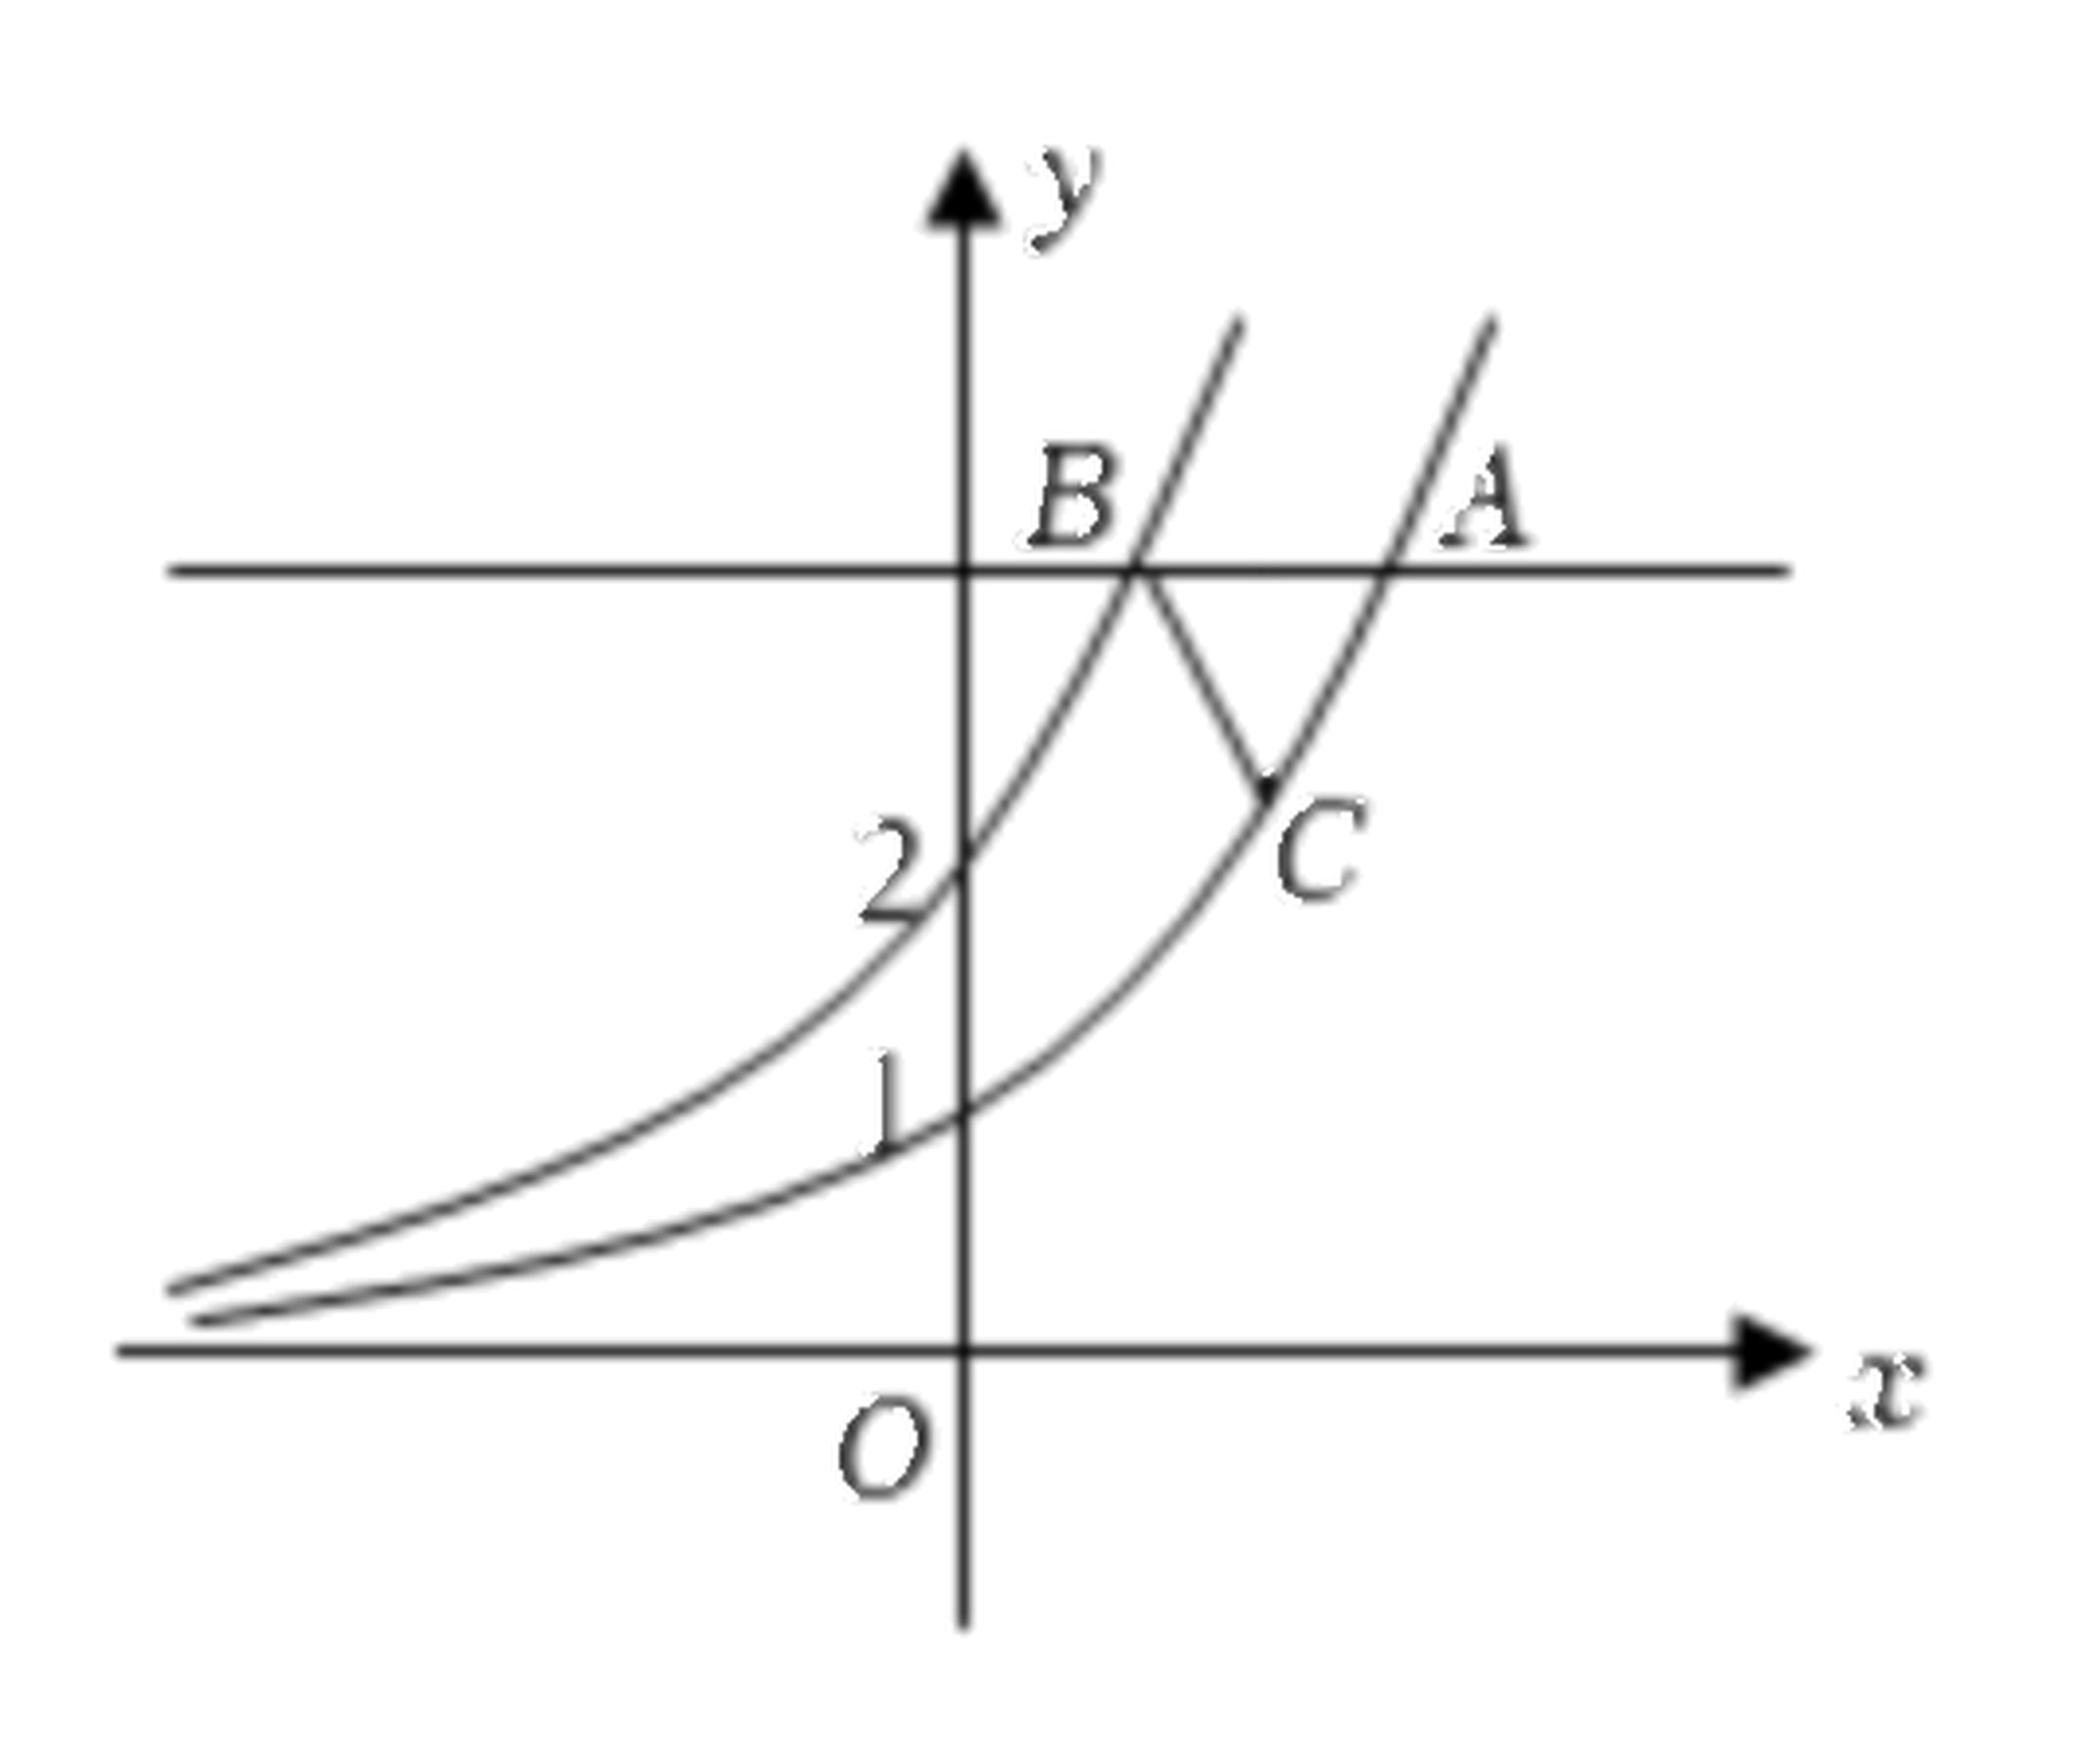
\includegraphics[width=0.40\textwidth]{figures/gao150_q11.png}
\end{center}

\ifanswer
\solbegin
\step{设直线 $l$ 的方程为 $y=a(a>0)$，}
\step{由 $2^x=a$，得 $x=\log_2 a$，所以 $A(\log_2 a,a)$，}
\step{由 $2^{x+1}=a$，得 $x=\log_2 a-1$，所以 $B(\log_2 a-1,a)$，所以 $\lvert AB\rvert=1$，}
\step{取 $AB$ 的中点 $D$，连接 $CD$，如图所示，}
\step{因为 $\triangle ABC$ 为等边三角形，则 $CD\perp AB$，且 $\lvert CD\rvert=\dfrac{\sqrt3}{2}$，}
\step{所以 $C\left(\log_2 a-\dfrac{1}{2},a-\dfrac{\sqrt3}{2}\right)$，}
\step{因为点 $C$ 在函数 $y=2^x$ 的图像上，所以 $a-\dfrac{\sqrt3}{2}=2^{\log_2 a-\frac{1}{2}}=\dfrac{a}{\sqrt2}$，}
\step{解得 $a=\dfrac{\sqrt3}{2-\sqrt2}=\dfrac{\sqrt3(2+\sqrt2)}{4-2}=\sqrt3+\dfrac{\sqrt6}{2}$，}
\step{所以点 $C$ 的纵坐标为 $a-\dfrac{\sqrt3}{2}=\dfrac{\sqrt3+\sqrt6}{2}$.}
\solend
\fi

% === Q12 === 解析配图（高斯函数方格阴影，仅答案版出）；"数学王子"弯引号；cases 块整体算一个印刷行；解析 4 行
\item 小玲在研究数学发展史，特别崇拜近代数学奠基者之一、享有“数学王子”称号的德国数学家高斯. 为了纪念高斯，我们把取整函数 $y=[x]$ 称为高斯函数，其中 $[x]$ 表示不超过 $x$ 的最大整数，如 $[1.1]=1$，$[-1.1]=-2$，则点集 $P=\{(x,y)\mid [x]^2+[y]^2=1\}$ 所表示的平面区域的面积为\blankline[4.4em].

\ifanswer
\solbegin
\step{$[x]^2+[y]^2=1$ 由 $\begin{cases}[x]=0\\ {[y]=-1}\end{cases}$ 或 $\begin{cases}[x]=0\\ {[y]=1}\end{cases}$ 或 $\begin{cases}[x]=-1\\ {[y]=0}\end{cases}$ 或 $\begin{cases}[x]=1\\ {[y]=0}\end{cases}$ 四个平面区域组成，}
\step{即 $\begin{cases}0\leqslant x<1\\ -1\leqslant y<0\end{cases}$ 或 $\begin{cases}0\leqslant x<1\\ 1\leqslant y<2\end{cases}$ 或 $\begin{cases}-1\leqslant x<0\\ 0\leqslant y<1\end{cases}$ 或 $\begin{cases}1\leqslant x<2\\ 0\leqslant y<1\end{cases}$，}
\step{作出平面区域如图所示，平面区域由四个边长为 $1$ 的正方形组成，}
\begin{center}
% 高斯函数 [x]^2+[y]^2=1 方格阴影区域图取 04 页顶部，去粉色水印、去色、4× LANCZOS 放大；仅答案版出
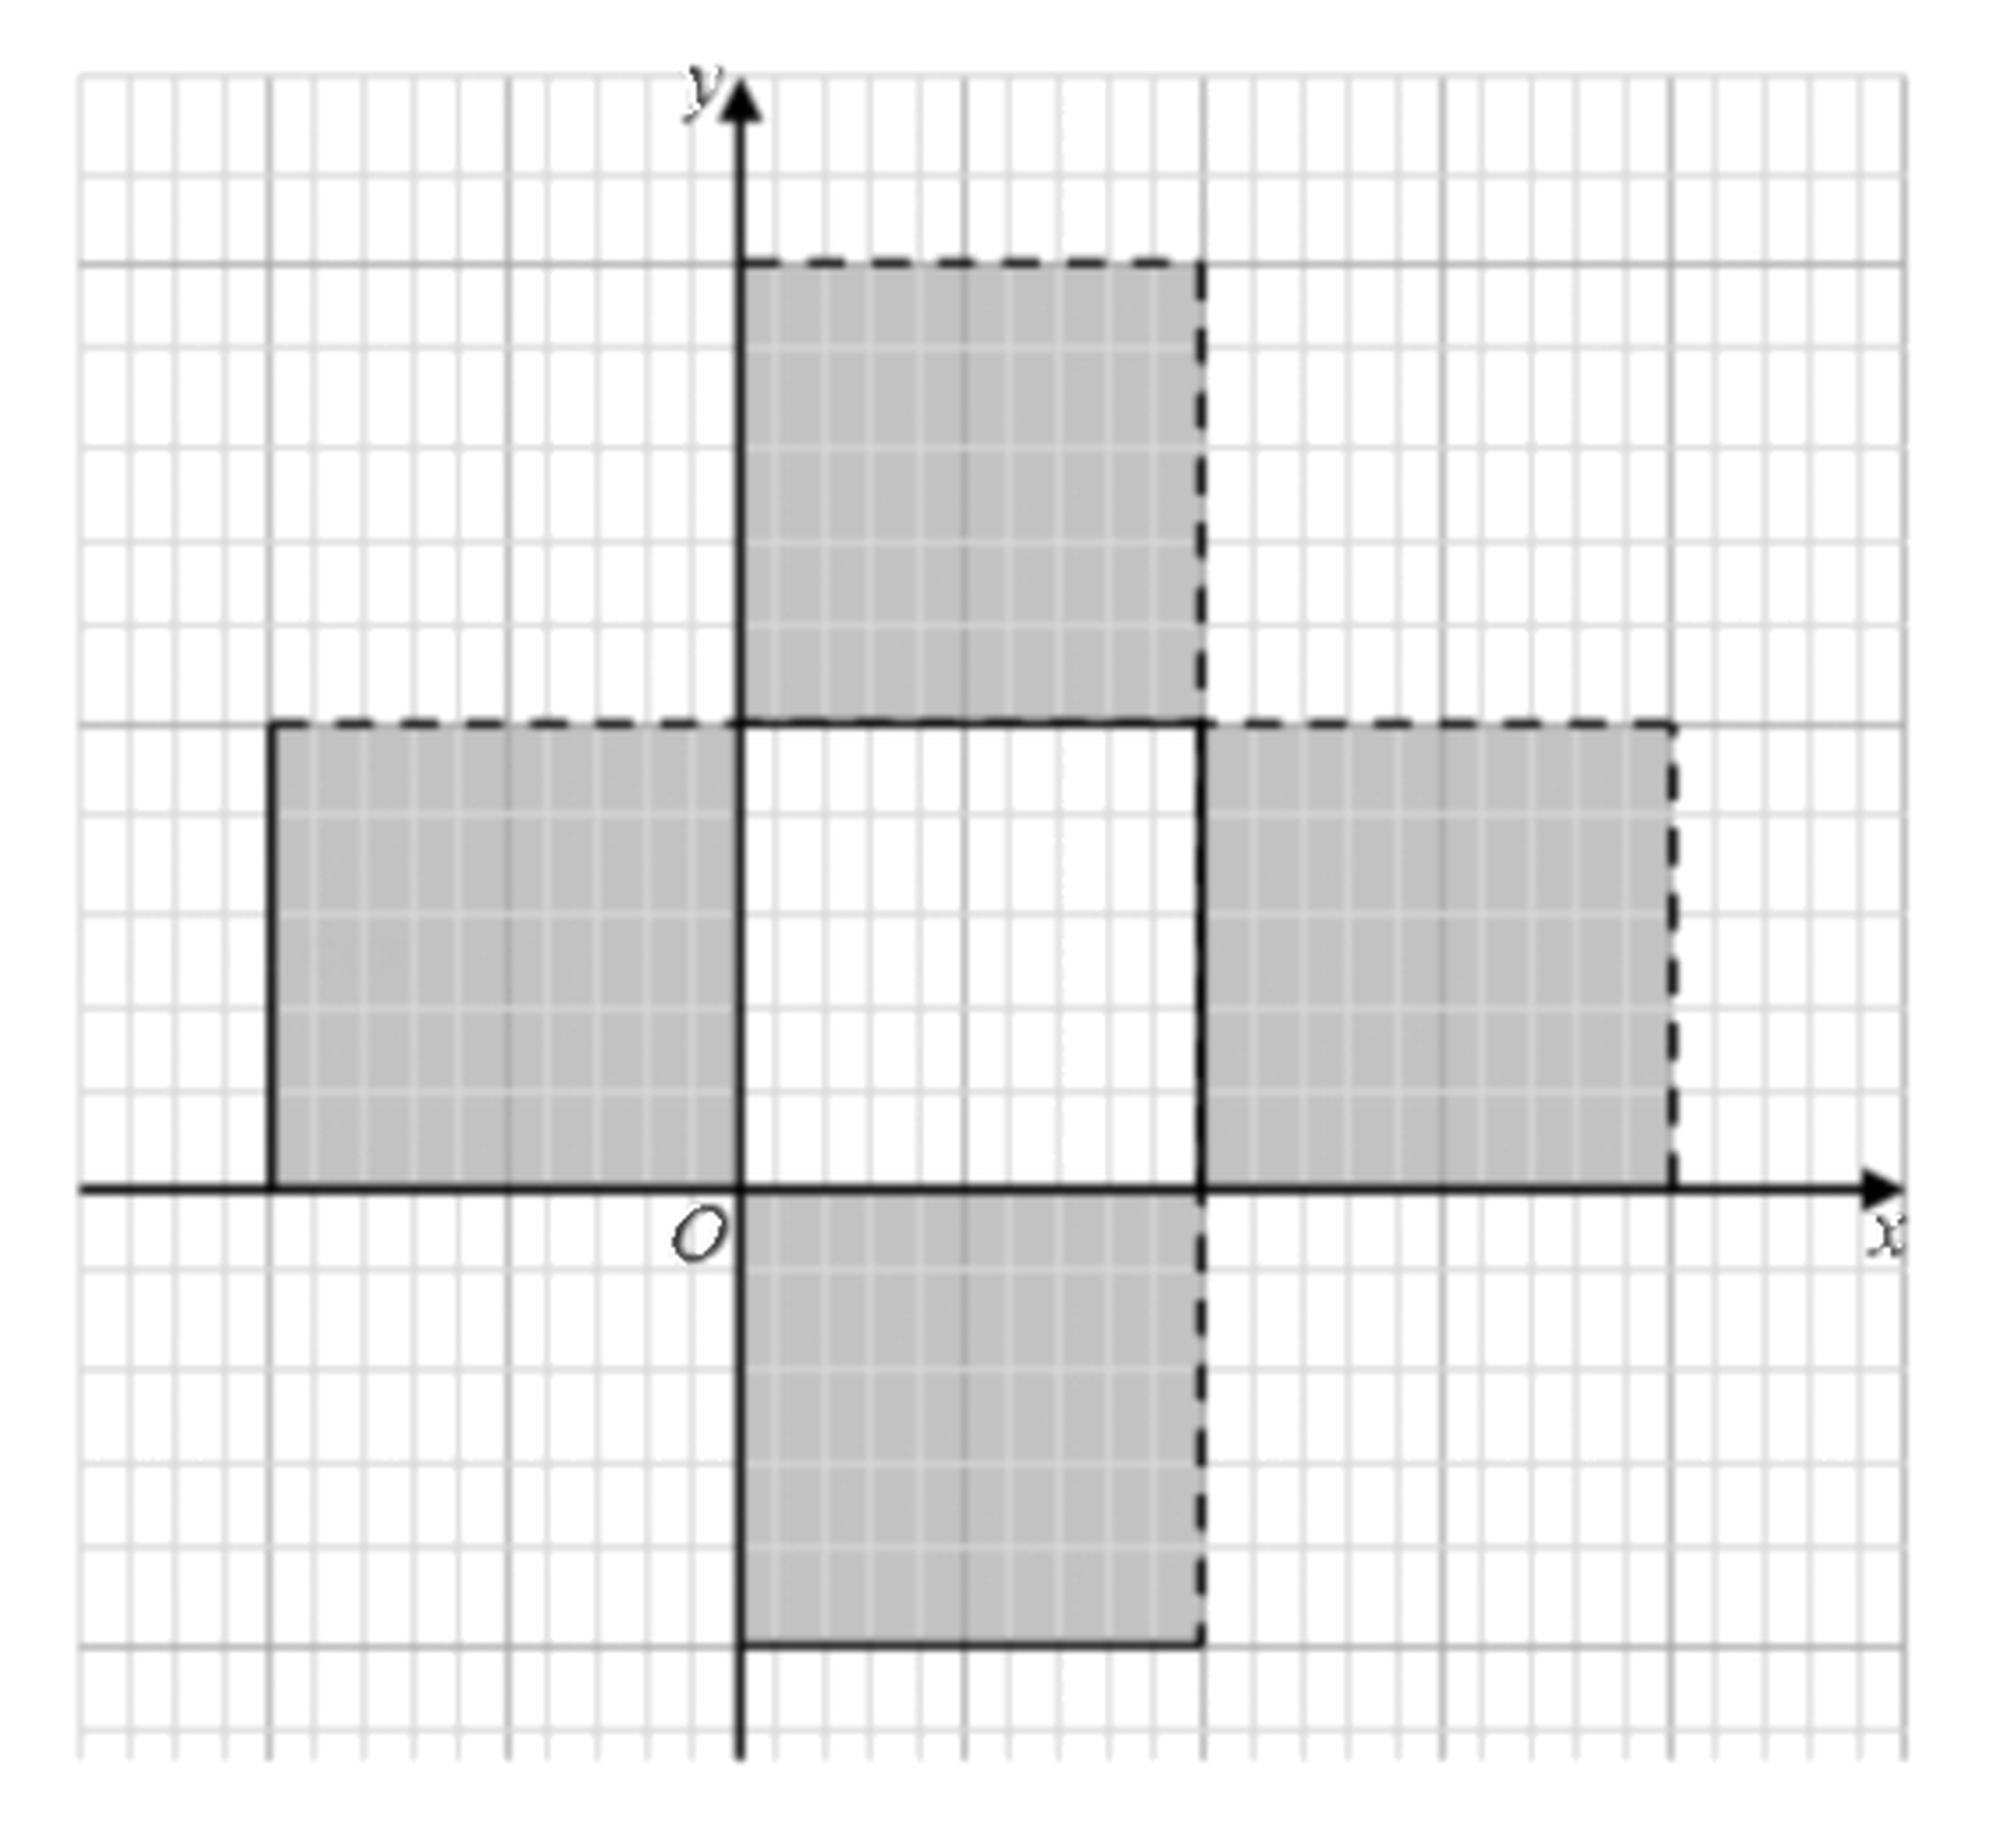
\includegraphics[width=0.34\textwidth]{figures/gao150_q12.png}
\end{center}
\step{总面积为 $1\times4=4$.}
\solend
\fi

\end{enumerate}

\bigsec{二、选择题}

\begin{enumerate}
\setcounter{enumi}{12}

% === Q13 === 答案在解析末句"故选 C"；括号 \mbox{（\quad）} 留空；四选项一行；解析 1 行
\item 设 $x\ne0$，则 $3^{\log_9 x^2}$ 的化简结果是\mbox{（\quad）}

\keepwithprev
A. $x$\qquad B. $\dfrac{1}{x}$\qquad C. $\lvert x\rvert$\qquad D. $\dfrac{1}{\lvert x\rvert}$

\ifanswer
\solbegin
\step{$3^{\log_9 x^2}=3^{\log_3\lvert x\rvert}=\lvert x\rvert$，故选 $C$.}
\solend
\fi

% === Q14 === 题目配图（两函数图像，三版都出）；\needvspace{8cm} 守卫放 \item 之前；"图像"照录；四选项两行两列；解析 2 行，故选 B
\needvspace{8cm}
\item 设 $a>0$ 且 $a\ne1$，$b\in\R$. 若函数 $y=a^{-\lvert x\rvert}$ 与 $y=x^b$ 的大致图像如图所示，则\mbox{（\quad）}

\keepwithprev
A. $0<a<1<b$\qquad\qquad B. $a>1$ 且 $b>1$

C. $0<a<1$ 且 $0<b<1$\qquad\qquad D. $0<b<1<a$

\begin{center}
% 两函数 y=a^{-|x|} 与 y=x^b 大致图像取 04 页右侧，去粉色水印、去色、4× LANCZOS 放大；三版都出
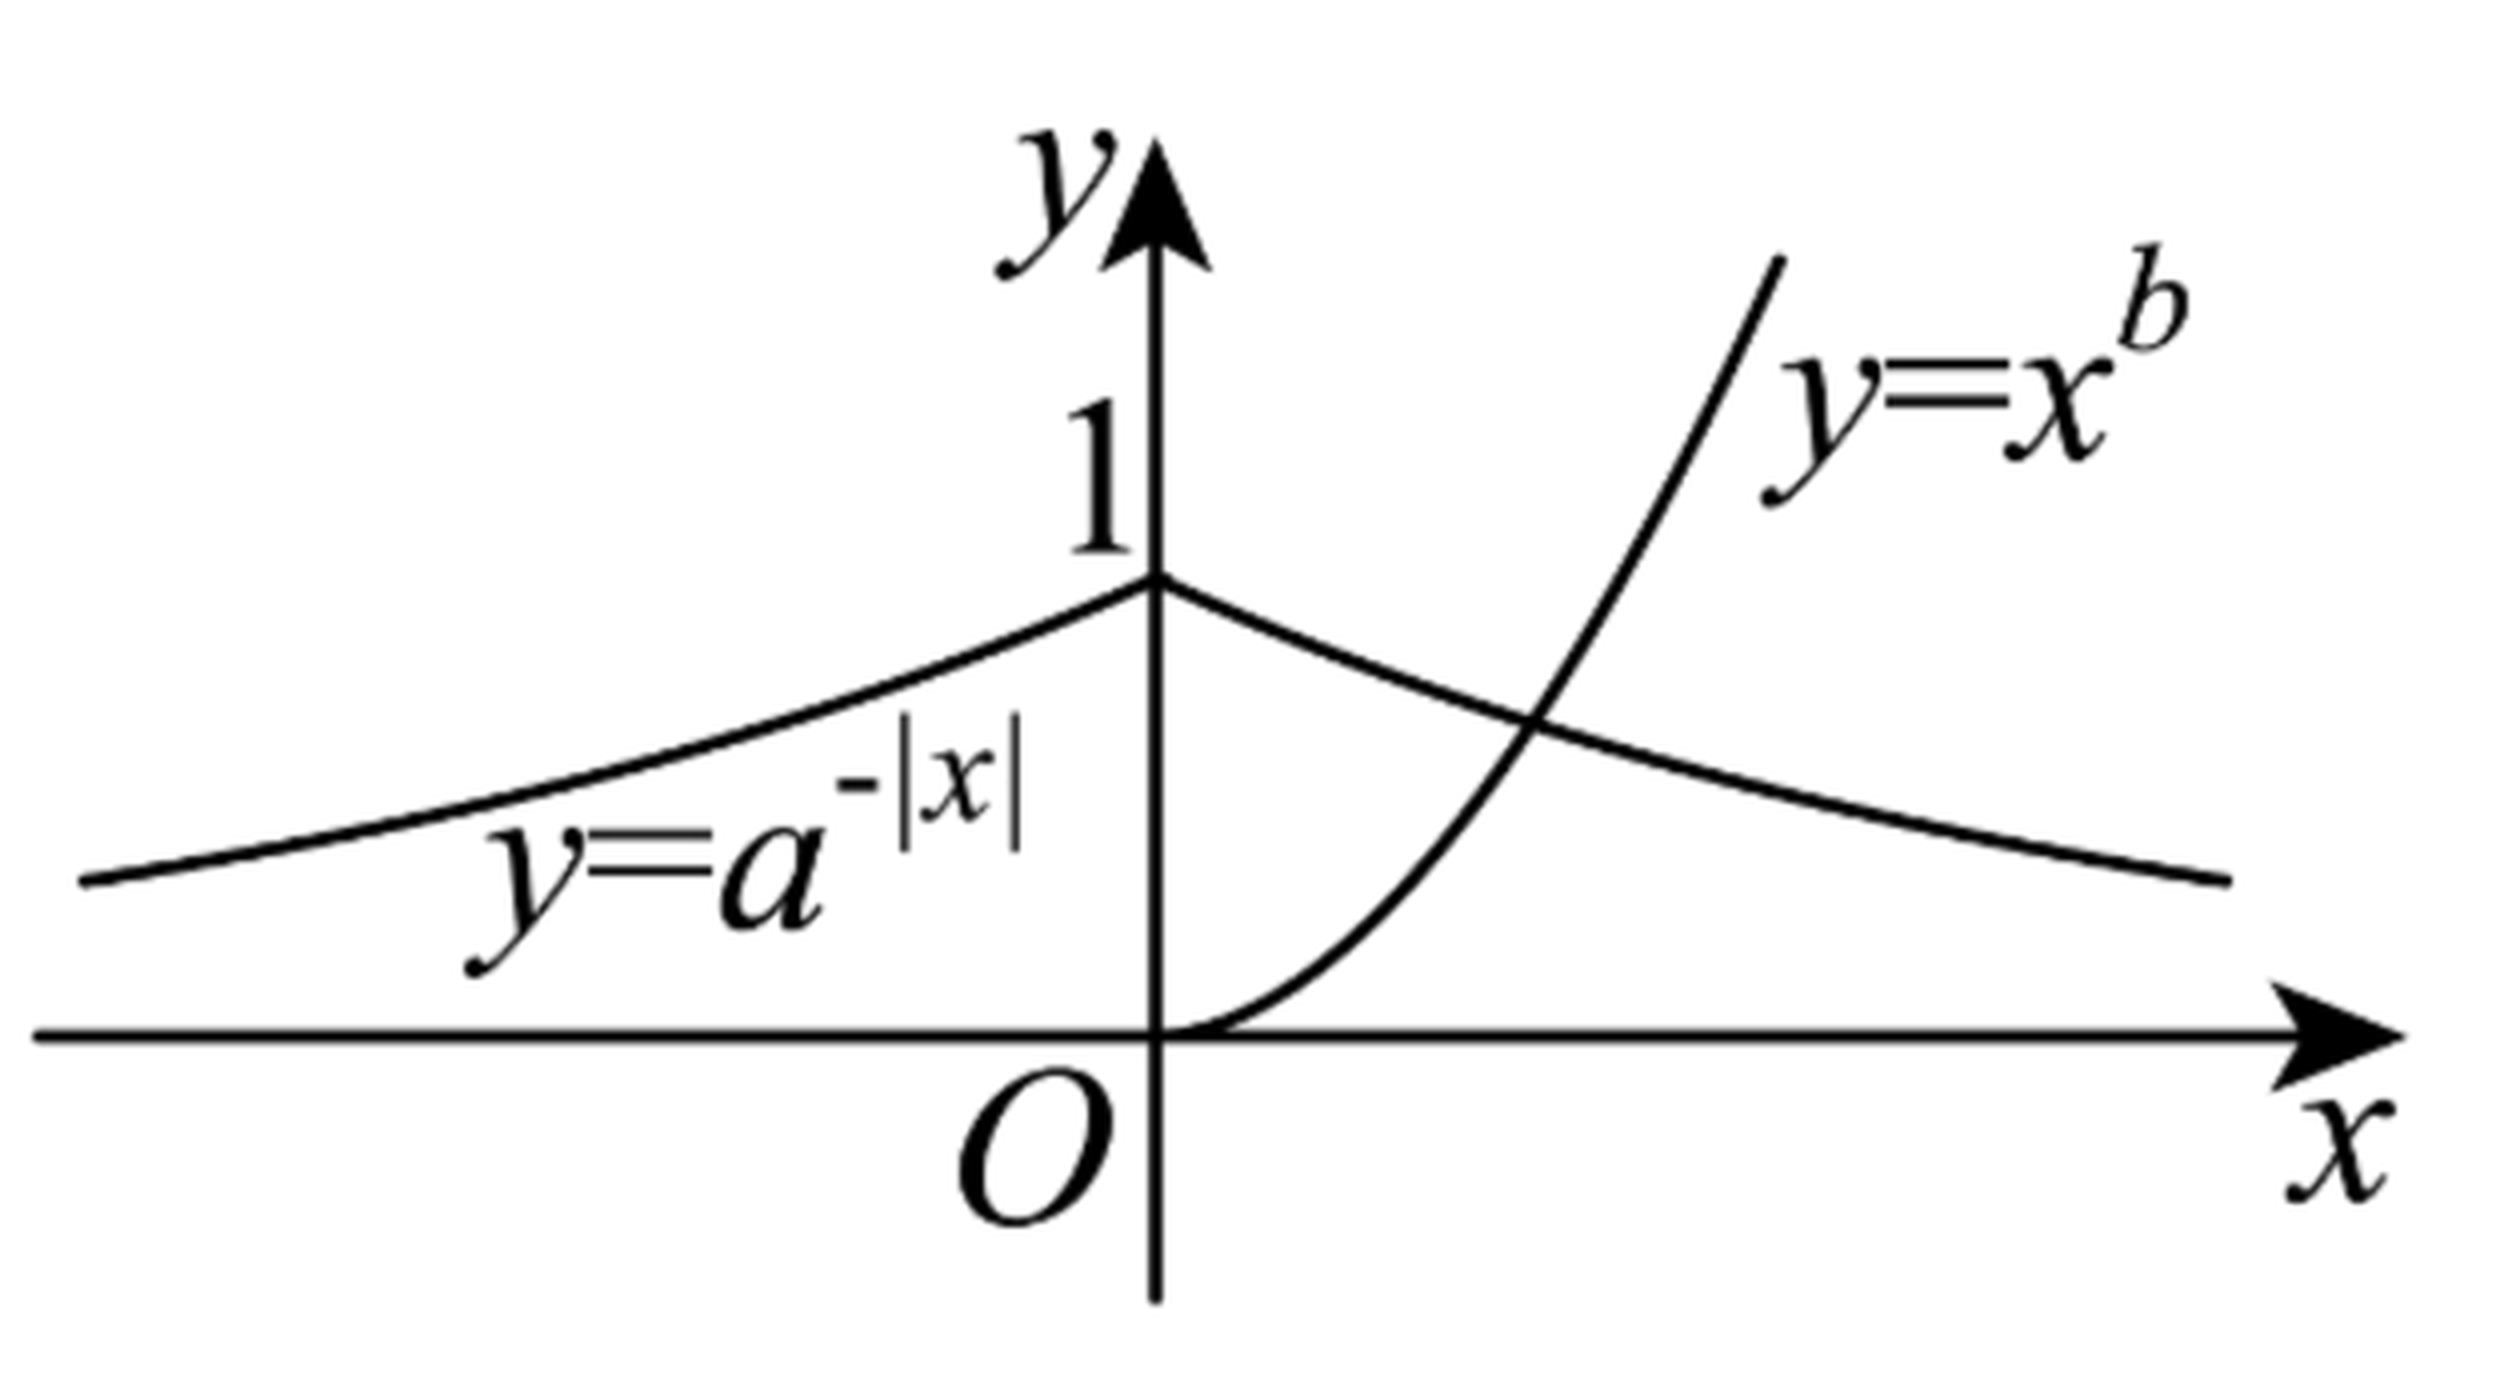
\includegraphics[width=0.40\textwidth]{figures/gao150_q14.png}
\end{center}

\ifanswer
\solbegin
\step{在 $(0,+\infty)$ 上，$y=a^{-x}$ 严格递减，得 $a>1$；}
\step{幂函数 $y=x^b$ 的图像递增且向上弯曲，得 $b>1$；故选 $B$.}
\solend
\fi

% === Q15 === "算术平均值／算术平均数"两处不同照录；四选项两行两列；解析 5 行（续 05 页顶），故选 B
\item 已知两个正数的算术平均值不小于它们的几何平均值，类比有以下结论：三个正数的算术平均数不小于它们的几何平均数，即当 $a,b,c$ 为正实数时，$\dfrac{a+b+c}{3}\geqslant\sqrt[3]{abc}$，当且仅当 $a=b=c$ 时等号成立. 利用上述结论，下列选项中判断正确的是\mbox{（\quad）}

\keepwithprev
A. 若 $x>0$，则 $2x+\dfrac{1}{x^2}\geqslant\dfrac{27}{8}$\qquad\qquad B. 若 $x>0$，则 $x^2+\dfrac{2}{x}\geqslant3$

C. 若 $0<x<1$，则 $x^2(1-x)\geqslant\dfrac{1}{9}$\qquad\qquad D. 若 $0<x<1$，则 $x^2(1-x)\leqslant\dfrac{1}{9}$

\ifanswer
\solbegin
\step{A：取 $x=1$，$2x+\dfrac{1}{x^2}=3<\dfrac{27}{8}$，错误.}
\step{B：$x^2+\dfrac{2}{x}=x^2+\dfrac{1}{x}+\dfrac{1}{x}\geqslant3\sqrt[3]{x^2\cdot\dfrac{1}{x}\cdot\dfrac{1}{x}}=3$，当且仅当 $x=1$ 时取等号，正确.}
\step{C：取 $x=\dfrac{1}{3}$，$x^2(1-x)=\dfrac{2}{27}<\dfrac{1}{9}$，错误.}
\step{D：取 $x=\dfrac{2}{3}$，$x^2(1-x)=\dfrac{4}{27}>\dfrac{1}{9}$，错误.}
\step{故选 $B$.}
\solend
\fi

% === Q16 === "完美集"新定义（弯引号、引号外空格照录）；圈数字①②文本模式；$n\in\N$；四选项两行两列；解析 9 行（6 行 05 页＋3 行 06 页顶），故选 A
\item 已知有限集 $A=\{a_1,a_2,\cdots,a_n\}$（$n\geqslant2$，$n\in\N$）. 若 $A$ 中元素 $a_i$（$i=1,2,\cdots,n$）满足 $a_1+a_2+\cdots+a_n=a_1\cdot a_2\cdots a_n$，就称 $A$ 为 “完美集”. 现有以下两个命题：

①恰有两个元素的 “完美集” 有无穷多个；

②若 $a_i$ 均为正整数，则 “完美集” $A$ 有且只有一个，且 $n=3$.

则\mbox{（\quad）}

\keepwithprev
A. ①和②都是真命题\qquad\qquad B. ①和②都是假命题

C. ①是真命题，②是假命题\qquad\qquad D. ①是假命题，②是真命题

\ifanswer
\solbegin
\step{①由 $a+b=ab\Leftrightarrow(a-1)(b-1)=1$，任取 $a>2$，则 $b=1+\dfrac{1}{a-1}\in(1,2)$，}
\step{得到无穷多个不同的完美集，①真.}
\step{②设 $1\leqslant a_1<a_2<\cdots<a_n$，则 $a_i\geqslant i$.}
\step{若 $n=2$，则 $(a_1-1)(a_2-1)=1$，只能有 $a_1=a_2=2$，与元素互异矛盾.}
\step{若 $n\geqslant4$，则 $a_1a_2\cdots a_n\geqslant a_2a_{n-1}a_n\geqslant2(n-1)a_n>na_n\geqslant a_1+\cdots+a_n$，矛盾.}
\step{当 $n=3$ 时，若 $a_1\geqslant2$，则 $a_1a_2a_3\geqslant6a_3>3a_3\geqslant a_1+a_2+a_3$，矛盾.}
\step{因此 $a_1=1$，$(a_2-1)(a_3-1)=2$，结合 $a_2<a_3$ 得 $a_2=2$，$a_3=3$.}
\step{唯一的完美集为 $\{1,2,3\}$，②真.}
\step{故选 $A$.}
\solend
\fi

\end{enumerate}

\bigsec{三、解答题}

\begin{enumerate}
\setcounter{enumi}{16}

% === Q17 === \varnothing 空集、$B\subseteq A$ 带下划线照录；弯引号内空格照录；解析 7 行
\item 设 $a,b\in\R$. 已知集合 $A=\{x\mid ax^2+3x-a>3\}$，$B=\{x\mid bx=1\}$.

(1) 若 $A=(1,2)$，求 $a$ 的值；

(2) 若 $a=0$，且 “ $x\in A$ ” 是 “ $x\in B$ ” 的必要非充分条件，求 $b$ 的取值范围.

\ifanswer
\solbegin
\step{(1) $A=(1,2)$，则 $a<0$，且 $1,2$ 是方程 $ax^2+3x-a-3=0$ 的两根.}
\step{由 $4a+6-a-3=0$，得 $a=-1$，此时不等式为 $-(x-1)(x-2)>0$，}
\step{解集确为 $(1,2)$.}
\step{(2) $a=0$ 时，$A=(1,+\infty)$，题意等价于 $B\subseteq A$ 且 $B\ne A$.}
\step{当 $b=0$ 时，$B=\varnothing$，符合条件.}
\step{当 $b\ne0$ 时，$B=\left\{\dfrac{1}{b}\right\}$，条件等价于 $\dfrac{1}{b}>1$，解得 $0<b<1$.}
\step{因此 $b$ 的取值范围为 $[0,1)$.}
\solend
\fi

% === Q18 === $p\in\Z$；"图像"（像，有亻）照录；指数 $-2p^2+5p$；解析 8 行（(1) 首行 06 页末＋2 行 07 页顶、(2) 5 行 07 页）
\item 设 $p\in\Z$，已知 $f(x)=x^{-2p^2+5p}$.

(1) 若幂函数 $y=f(x)$ 的图像关于原点成中心对称，且满足 $f(3)<f(4)$，求 $p$ 的值；

(2) 当 $p=-2$ 时，求满足 $f(2x+3)<f(x-4)$ 的 $x$ 的取值范围.

\ifanswer
\solbegin
\step{(1) 图像关于原点成中心对称，得整数 $-2p^2+5p$ 为奇数.}
\step{由 $f(3)<f(4)$，得 $-2p^2+5p>0\Leftrightarrow0<p<\dfrac{5}{2}$，}
\step{结合 $p\in\Z$，得 $p=1$ 或 $p=2$，对应指数分别为 $3$、$2$，所以 $p=1$.}
\step{(2) 当 $p=-2$ 时，$f(x)=\dfrac{1}{x^{18}}$，定义域为 $\{x\in\R\mid x\ne0\}$.}
\step{原不等式要求 $x\ne-\dfrac{3}{2}$ 且 $x\ne4$，}
\step{此时 $\dfrac{1}{(2x+3)^{18}}<\dfrac{1}{(x-4)^{18}}\Leftrightarrow\lvert 2x+3\rvert>\lvert x-4\rvert\Leftrightarrow(2x+3)^2>(x-4)^2$，}
\step{因此 $(x+7)(3x-1)>0\Leftrightarrow x<-7$ 或 $x>\dfrac{1}{3}$，}
\step{排除 $x=4$，得 $x\in(-\infty,-7)\cup\left(\dfrac{1}{3},4\right)\cup(4,+\infty)$.}
\solend
\fi

% === Q19 === $a\in\R$、$g(x)=f(2x+1)+a\cdot f(x)+2$；解析 6 行（(2) 末两行续 08 页顶）
\item 已知 $f(x)=2^x$.

(1) 求方程 $f(2x)-f(x)=6$ 的解；

(2) 设 $a\in\R$，$g(x)=f(2x+1)+a\cdot f(x)+2$，若对于任意 $x\in[-1,1]$，均有 $g(x)\geqslant1$，求 $a$ 的取值范围.

\ifanswer
\solbegin
\step{(1) 令 $t=2^x>0$，则 $t^2-t-6=(t-3)(t+2)=0$，}
\step{由 $t>0$ 得 $t=3$，所以 $x=\log_2 3$.}
\step{(2) 令 $t=2^x$，则 $t\in\left[\dfrac{1}{2},2\right]$，且 $g(x)\geqslant1\Leftrightarrow2t^2+at+1\geqslant0\Leftrightarrow a\geqslant-\left(2t+\dfrac{1}{t}\right)$，}
\step{由基本不等式得 $2t+\dfrac{1}{t}\geqslant2\sqrt{2t\cdot\dfrac{1}{t}}=2\sqrt2$，}
\step{当且仅当 $t=\dfrac{1}{\sqrt2}\in\left[\dfrac{1}{2},2\right]$ 时等号成立，}
\step{因此 $-\left(2t+\dfrac{1}{t}\right)$ 的最大值为 $-2\sqrt2$，所求范围为 $a\in[-2\sqrt2,+\infty)$.}
\solend
\fi

% === Q20 === "极闭集"新定义、3 问，全卷末题；$M\subseteq(0,+\infty)$ 带下划线照录；自定义运算 $x*y$ 星号照录；解析 13 行（9 行 08 页＋4 行 09 页上半）
\item 对于非空实数集 $M\subseteq(0,+\infty)$，若满足以下两个条件：

① $M$ 中至少含有 $2$ 个元素，且 $1\notin M$；

②对于 $M$ 中任意两个不相等的元素 $x$、$y$，定义 $x*y=\dfrac{xy+1}{x+y}$，且 $x*y\in M$.

则称 $M$ 为 “极闭集”.

(1) 分别判断集合 $A=\left\{\dfrac{1}{2},3\right\}$ 与集合 $B=(1,+\infty)$ 是否为 “极闭集” （无需理由）；

(2) 若 $M$ 是 “极闭集”，证明：$M$ 中不可能所有元素都小于 $1$；

(3) 证明：不存在任何有限集是 “极闭集”.

\ifanswer
\solbegin
\step{(1) $A$ 不是 “极闭集”，$B$ 是 “极闭集”.}
\step{(2) 假设 $M$ 中所有元素都小于 $1$，取其中两个不相等的元素 $x$、$y$，}
\step{则 $x*y-1=\dfrac{(1-x)(1-y)}{x+y}>0$，}
\step{这与 $x*y\in M$ 且 $M$ 中所有元素都小于 $1$ 矛盾.}
\step{(3) 假设有限集 $M$ 是 “极闭集”，}
\step{由 (2) 及 $1\notin M$，得 $M$ 中存在大于 $1$ 的元素.}
\step{若 $M$ 中有小于 $1$ 的元素，取其中最大的一个为 $a$，另取 $b\in M$ 且 $b>1$，}
\step{则 $a*b-a=\dfrac{1-a^2}{a+b}>0, a*b-1=\dfrac{(a-1)(b-1)}{a+b}<0$，}% 半角逗号在两个数学式组之间，全稿惯例、非笔误，照录
\step{于是 $a<a*b<1$ 且 $a*b\in M$，与 $a$ 的最大性矛盾.}
\step{若 $M$ 中没有小于 $1$ 的元素，则 $M\subseteq(1,+\infty)$.}
\step{取 $a=\min M$，另取 $b\in M$ 且 $b\ne a$，则 $a*b-a=\dfrac{1-a^2}{a+b}<0$，}
\step{于是 $a*b<a$ 且 $a*b\in M$，与 $a$ 的最小性矛盾.}
\step{因此不存在任何有限集是 “极闭集”.}
\solend
\fi

\end{enumerate}

\end{document}
"
% 紧凑版：xelatex "\def\iscompact{1}% 高一150_曹杨二中_期中.tex
%   —— 高一上数学"2026-2027 年曹杨二中高一上期中"（试卷版/答案版/紧凑版）
% 试卷版：xelatex 高一150_曹杨二中_期中.tex
% 答案版：xelatex "\def\isanswer{1}\input{高一150_曹杨二中_期中.tex}"
% 紧凑版：xelatex "\def\iscompact{1}\input{高一150_曹杨二中_期中.tex}"
%
% ① 原始材料：微信公众号"魔都数学加油站"文章，连载"27学年高一150"，原文标题
% "27学年高一150——2026-2027年上海市曹杨二中高一上期中"；
% 原文链接：https://mp.weixin.qq.com/s/xlQxmik8TZXR87RC6MnCrw 。
% 正文为 9 张 PNG 页（01/02/04/06/07/09 为 2560×3620，03/05/08 为 4762×6735，
% 同一篇各页分辨率混排，逐页按各自分辨率裁图核对，别按预览比例换算裁框）。
% 体例：讲评版——全 18 题均印【解析】（逐题核实，见 ② ②）。
% 题目、答案、解析均据原图转录；卷面粉红色/红色水印"魔都数学加油站"及公众号页脚未录入。
% 全卷插图清单（逐页通读 9 页确认）：3 幅——
%   · Q11 题目配图（指数函数曲线图，02 页右侧：x/y 轴、O、y=2^x 与 y=2^{x+1}
%     两曲线、A/B/C 三点、刻度 1/2、等边三角形 ABC），三版都出，裁 figures/gao150_q11.png；
%   · Q12 解析配图（高斯函数取整 [x]^2+[y]^2=1 方格阴影区域图，04 页顶部：4 个边长 1
%     的正方形组成的十字形阴影），解析"作出平面区域如图所示"处，仅答案版出，
%     放 \ifanswer 内 \step 之间，裁 figures/gao150_q12.png；
%   · Q14 题目配图（两函数 y=a^{-|x|} 与 y=x^b 大致图像，04 页右侧：x/y 轴、O、
%     y 轴刻度 1、一递减曲线一递增上翘曲线），三版都出，裁 figures/gao150_q14.png；
%   其余各页逐页确认无其它题目配图、无表格；Q11/Q12 解析"如图所示"对应的就是上列
%   已裁的图，不重复裁；09 页上半为 Q20(3) 解析续尾、下半仅水印、无正文。
%   3 图均取自原卷截图，去粉色水印、去色、4× LANCZOS 放大。
%
% 卷首标题：原卷印作"2026-2027 年曹杨二中高一上期中"，年份区间按全稿惯例排 en dash；
% 原卷卷面未印副标题，本稿按同期中卷知识模块口径补出"集合与常用逻辑用语、不等式、函数"。
%
% 题号体例（逐页核实定稿）：本卷共 18 题——一、填空题 3—12（10 题）、
% 二、选择题 13—16（4 题）、三、解答题 17—20（4 题）。
% 三节分别 \setcounter{enumi}{2}／{12}／{16}。原卷从第 3 题起、无第 1、2 题，
% 本稿保留原题号；全卷末题为第 20 题（"极闭集"新定义、3 问），无 Q21、无附加题节。
%
% ② 与原卷的排版差异：
%   ① 原文从第 3 题起，本稿保留原题号；共 18 题三节，解答题只有 4 题到 20；
%   ② 全 18 题均印【解析】，用 \solbegin…\solend；逐题核实无只印【答案】或
%      答案印题干括号内的题；四道选择题答案在解析末句"故选 X"（Q13 选 C、
%      Q14 选 B、Q15 选 B、Q16 选 A，逐个放大复核）、括号 \mbox{（\quad）} 留空、
%      不另提 \ans{}；答案版【答案】/【解析】标记数 = 18 = 全卷题数；
%   ③ 原卷卷面未印副标题，本稿按知识模块口径补出；
%   ④ 原卷填空横线按全稿惯例排 \blankline[4.4em]；选择题括号排 \mbox{（\quad）}、
%      选项段前按惯例加 \keepwithprev；解答题不留作答区、不加 \anspace（原卷为讲评版）；
%   ⑤ 数集黑板粗体：Q4"m\in R"、Q5"a,b\in R"、Q6"a,b,c\in R"、Q7"a\in R"、
%      Q10"a\in R"、Q14"b\in R"、Q17"a,b\in R"、Q18"p\in Z"／定义域"x\in R"、
%      Q19"a\in R"、Q16"n\in N" 原卷印斜体 R/Z/N，按全稿惯例归一 \R／\Z／\N；
%      绝对值排 \lvert…\rvert（Q7 |x+4|+|x-3|、Q11 |AB|／|CD|、Q13 |x|、
%      Q18 |2x+3|／|x-4|），集合描述竖线排 \mid（Q3、Q12、Q17、Q18、Q20），
%      不等号按全稿惯例排 \leqslant／\geqslant；补集照原卷上划线排 \overline{A}
%      （Q3 题干＋解析共 2 处）；空集符号 \varnothing（Q17 解析(2)）；
%      子集 \subset（单线⊂）／\subseteq（带下划线⊆）逐处照录，本卷 3 处子集
%      符号均印带下划线 ⊆、照录 \subseteq（Q20 题干、Q20 解析(3)、Q17 解析(2)，
%      见 ④），无 \subset 用例；
%   ⑥ 判别式 Δ/△：逐页通读 9 页，本卷无一元二次判别式算式，故无 Δ/△ 混用可照录
%      （"高 \Delta／扁 \triangle"口径备查，参照 高一142／144／145／146／148／149
%      头注④）；本卷仅 Q11 题干与解析共 2 处几何三角形符号 △ABC，逐处放大并排
%      确认两处同形、印近等边粗线三角（非判别式），照录 \triangle（见 ④）；
%   ⑦ 中文弯引号照录：Q12"数学王子"、Q16"完美集"（题干＋①②两命题，引号外
%      留空格）、Q17" x∈A "" x∈B "（引号内空格）、Q20"极闭集"（题干条件、
%      三问与解析，引号外留空格）；注释里一律 ASCII 引号；数学式内 CJK 用 \text{}
%      （Q3 集合描述"且"用 \text{ 且 }）；
%   ⑧ 半角逗号在数学组之间是全稿惯例、非笔误，逐处照录（Q17 解析"1,2 是方程…
%      两根"、Q20 解析(3)">0, a*b-1=…<0" 两式之间等）；行末西文句点 ASCII `.`；
%      行中全角逗号／顿号照录（Q12"之一、享有"、Q18 解析"3、2"、Q20"x、y"）；
%   ⑨ "图像／图象"逐处放大核：全卷 9 处均印"图像"（像，有亻）、未见"图象"——
%      Q4 题干 1、Q11 题干 2＋解析 1、Q14 题干 1＋解析 1、Q18 题干 1＋解析 1；
%      同卷"第二象限""象限"用"象"（无亻）。逐处照录未统一改动（放大 01/02/04/06
%      页 /tmp/gao150/z/p01_q4_tuxiang2.png、p04_q14_tuxiang2.png、
%      p02_q11_lines.png 确认）；子题标号 (1)(2)(3) 半角括号照录；圈数字①②
%      在文本模式（Q16 两命题与解析、Q20 两条件与三问及解析）按 common.sty
%      划入 CJK 字符类渲染，进数学式用 \text{①}；
%   ⑩ Q20 新定义 x*y=\dfrac{xy+1}{x+y} 的 * 是自定义运算（星号），照录；
%      \left…\right 不得拆到不同 $…$ 组（Q19"\left(2t+\frac1t\right)"、
%      Q20 题干"A=\left\{\frac12,3\right\}"等）；Q8 嵌套根号
%      \sqrt{\frac2x+\frac{16}{1-2x}}、Q9 对数连加 \log_2 A 等复杂式照录别简化；
%   ⑪ 一条 \step = 原卷解析的一个印刷行，cases 块整体算一个印刷行；别并折行、
%      别拆行。Q4 三行、Q8 五行、Q11 九行、Q12 四行（两行各含四个 cases 块）、
%      Q15 五行、Q16 九行、Q18 八行、Q20 十三行均按印刷行逐条断，不丢行；
%   ⑫ 配图：Q11／Q14 题目配图（三版都出）放 \item 内题干之后 \begin{center}，
%      大图块加 \needvspace{8cm} 守卫把整块推走（守卫放 \item 之前，见
%      高一145 Q14/Q20 成例与切页审计 B 类坑）；Q12 解析配图（仅答案版出）
%      放 \ifanswer 内 \solbegin…\solend 的 \step 之间（高一73 第16题成例）；
%   ⑬ 跨页续印按题合并：见 ⑥；
%   ⑭ 原卷解析内无红色"法一／法二"之类小标题，故本卷无 \stepm；红色水印
%      "魔都数学加油站"不录入；Q12 解析"作出平面区域如图所示"对应的图即
%      ① 所列 gao150_q12.png（04 页顶部），不重复裁；Q11 解析"如图所示"对应
%      题目配图 gao150_q11.png，不另裁。
%
% ③ 行数复核：一条 \step／\stepm = 原卷解析的一个印刷行，cases 块作一个印刷行计。
%   逐题数（主会话逐页核对定稿）：Q3：1；Q4：3；Q5：2；Q6：1；Q7：2；Q8：5；
%   Q9：1；Q10：3；Q11：9；Q12：4；Q13：1；Q14：2；Q15：5；Q16：9；
%   Q17：7；Q18：8；Q19：6；Q20：13。
%   合计 82 条 \step（本卷无 \stepm：解析内无红色"法一／法二"类小标题），
%   与原卷逐题印刷行相等。全卷 18 题均设 \solbegin…\solend，答案版
%   【答案】/【解析】标记数 = 18 = 全卷题数。
%
% ④ 判别式／三角形／子集符号结论（逐处放大原图照录、不得统一，主会话像素级复核）：
%   判别式：逐页通读 9 页，本卷无一元二次判别式 Δ/△ 算式（Q18 讨论幂函数指数
%     奇偶、不用判别式；Q9／Q19／Q20 亦无），头注 ② ⑥ 的"高 \Delta／扁 \triangle"
%     口径在本卷无对应处（参照 高一142／144／145／146／148／149 头注④，仅备查）。
%   几何三角形符号：Q11 题干"使得 △ABC 为等边三角形"（02 页末）与解析
%     "因为 △ABC 为等边三角形，则 CD⊥AB"（03 页）共 2 处，放大 02/03 页
%     /tmp/gao150/z/q11_tri_montage2.png 并排确认两处同形、印近等边粗线三角
%     （h/w≈0.98、非"高>宽"的判别式 \Delta），照录 \triangle（与 高一105
%     "使得 \triangle ABC 为等边三角形" 同短语成例、高一149 几何三角形照录
%     \triangle 口径一致），不引入 \Delta。
%   子集／补集：Q20 题干"$M\subseteq(0,+\infty)$"（08 页）、Q20 解析(3)
%     "则 $M\subseteq(1,+\infty)$"（09 页）、Q17 解析(2)"题意等价于 $B\subseteq A$
%     且 $B\ne A$"（06 页）共 3 处子集符号，逐处放大（/tmp/gao150/z/p08_q20_stem.png、
%     p09_q20_sub.png、p06_q17_sub.png）确认均印带下划线 ⊆，照录 \subseteq；
%     本卷未见单线 ⊂（\subset）之对应处。Q3 题干与解析共 2 处补集照原卷上划线
%     排 \overline{A}；Q17 解析(2) 空集印 ∅、照录 \varnothing（Q7"解集为空集"
%     为中文词、非符号，照录文字）；集合描述竖线 \mid；数集 \R／\Z／\N 归一见 ② ⑤。
%
% ⑤ 存疑照录（放大原图确认，照录未改、正文对应处另有 % 注）：
%   1. Q8 解析第 4 行"所以 $y=\frac1x+\frac{8}{1-2x}$ 的最小值为 18" —— 上文
%      并未定义 $y$，且题面求的是 $\sqrt{\frac2x+\frac{16}{1-2x}}$ 的最小值；
%      按上下文该行应为 $\frac1x+\frac{8}{1-2x}$ 的最小值为 18（$y$ 疑为原卷
%      衍字／笔误），放大 02 页 /tmp/gao150/z/p02_q8_y.png 确认，照录未改。
%   2. Q20 解析(3)"$a*b-a=\frac{1-a^2}{a+b}>0, a*b-1=\frac{(a-1)(b-1)}{a+b}<0$"
%      两式之间的逗号原卷印半角 ,（非全角），按全稿惯例"半角逗号在数学组之间"
%      照录未改（放大 08 页 /tmp/gao150/z/p08_q20_sol8.png 确认）。
%   3. Q15 题干"两个正数的算术平均值…几何平均值"与"三个正数的算术平均数…
%      几何平均数"两处"值／数"用字不同，逐处照录未统一（放大 04 页确认）。
%   4. "图像／图象"全卷 9 处均印"图像"（像，有亻）、未见"图象"，逐处放大核实
%      照录、未统一改动（见 ② ⑨）；本卷判别式 Δ/△ 无用例、几何三角形 2 处
%      照录 \triangle（见 ④）。
%   全卷除此 4 类外未发现其它笔误／自相矛盾处；18 题均印【解析】、无只印【答案】
%   或答案印题干括号内的题（见 ② ②）。
%
% ⑥ 跨页续印按题合并说明（逐页核实定稿）：Q3/4/5/6/7 题干＋解析在 01 页；
%   Q8 题干＋解析 5 行、Q9 题干＋解析 1 行在 02 页上半；Q10 题干＋解析 3 行
%   在 02 页下半；Q11 题干（前两行）＋配图在 02 页下半、题干续"三角形，则点 C
%   的纵坐标为___"与解析 9 行全在 03 页上半（解析"如图所示"对应题目配图）；
%   Q12 题干＋解析 4 行在 03 页下半，解析配图（方格阴影）续印在 04 页顶部；
%   "二、选择题"标题在 04 页中部；Q13 题干＋选项＋解析、Q14 题干＋选项＋
%   配图＋解析在 04 页；Q15 题干＋四选项在 04 页末、解析 5 行续 05 页上半；
%   Q16 题干＋①②两命题＋"则(  )"＋四选项＋解析前 6 行在 05 页、解析末 3 行
%   （"因此 a_1=1…②真""故选 A"）续 06 页顶部；"三、解答题"标题在 06 页；
%   Q17 题干(1)(2)＋解析(1) 3 行＋解析(2) 首行在 06 页、解析(2) 续 3 行
%   在 06 页下半；Q18 题干(1)(2)＋解析(1) 首行在 06 页末、解析(1) 续 2 行＋
%   解析(2) 5 行在 07 页上半；Q19 题干(1)(2)＋解析(1) 2 行＋解析(2) 前 2 行
%   在 07 页下半、解析(2) 末 2 行续 08 页顶部；Q20 题干（新定义＋①②两条件）
%   ＋三问＋解析(1)(2)(3) 前 9 行在 08 页、解析(3) 末 4 行续 09 页上半，
%   末行"因此不存在任何有限集是极闭集"为全卷收尾（09 页下半仅水印、无正文）。
%   本稿按题连排，不丢行、不并折行；全卷末题为第 20 题，无 Q21、无附加题节。
%
\documentclass[a4paper,11pt]{article}
\usepackage{common}

\begin{document}

\examtitlest[3]{2026--2027 年曹杨二中高一上期中}{集合与常用逻辑用语、不等式、函数}

\bigsec{一、填空题}

\begin{enumerate}
\setcounter{enumi}{2}

% === Q3 === 补集上划线 \overline{A}（题干＋解析各 1 处）；集合描述竖线 \mid、数学式内"且"用 \text{}；解析 1 行
\item 设全集 $U=\{1,2,3,4,5\}$，集合 $A=\{x\mid x^2-3x\leqslant0\text{ 且 }x\in U\}$，则 $\overline{A}=$\blankline[4.4em].

\ifanswer
\solbegin
\step{$x^2-3x\leqslant0\Leftrightarrow0\leqslant x\leqslant3$，所以 $A=\{1,2,3\}$，$\overline{A}=\{4,5\}$.}
\solend
\fi

% === Q4 === "图像"（像，有亻）逐处照录、同句"第二象限"用"象"（无亻）；解析 3 行
\item 设 $m\in\R$. 若幂函数 $y=(m^2-5m+1)x^{m+1}$ 的图像经过第二象限，则 $m=$\blankline[4.4em].

\ifanswer
\solbegin
\step{幂函数的系数为 1，故 $m^2-5m+1=1\Rightarrow m=0$ 或 $m=5$.}
\step{$m=0$ 时，$y=x$ 不经过第二象限；}
\step{$m=5$ 时，$y=x^6$ 经过第二象限，因此 $m=5$.}
\solend
\fi

% === Q5 === 解析 2 行
\item 设 $a,b\in\R$. 若 $a^2+\dfrac{b^2}{4}=1$，则 $ab$ 的最大值为\blankline[4.4em].

\ifanswer
\solbegin
\step{$1-ab=\left(a-\dfrac{b}{2}\right)^2\geqslant0$，即 $ab\leqslant1$；}
\step{当 $a=\dfrac{\sqrt2}{2}$，$b=\sqrt2$ 时取等号，最大值为 1.}
\solend
\fi

% === Q6 === 解析 1 行
\item 设 $a,b,c\in\R$. 若等式 $2x^2-3x-2=a(x-1)^2+b(x-1)+c$ 恒成立，则 $a-b+c=$\blankline[4.4em].

\ifanswer
\solbegin
\step{令 $x=0$，得 $a-b+c=-2$.}
\solend
\fi

% === Q7 === 绝对值 \lvert…\rvert；解析 2 行
\item 设 $a\in\R$. 若关于 $x$ 的不等式 $\lvert x+4\rvert+\lvert x-3\rvert<a$ 的解集为空集，则 $a$ 的取值范围是\blankline[4.4em].

\ifanswer
\solbegin
\step{$\lvert x+4\rvert+\lvert x-3\rvert\geqslant\lvert(x+4)-(x-3)\rvert=7$，当 $-4\leqslant x\leqslant3$ 时取等号.}
\step{原不等式的解集为空集当且仅当 $a\leqslant7$，即 $a\in(-\infty,7]$.}
\solend
\fi

% === Q8 === 嵌套根号 \sqrt{\frac{2}{x}+\frac{16}{1-2x}} 照录别简化；解析 5 行
\item 设 $x\in\left(0,\dfrac{1}{2}\right)$，则 $\sqrt{\dfrac{2}{x}+\dfrac{16}{1-2x}}$ 的最小值为\blankline[4.4em].

\ifanswer
\solbegin
\step{因为 $x\in\left(0,\dfrac{1}{2}\right)$，所以 $1-2x>0$，又 $2x+1-2x=1$，}
\step{所以 $\left(\dfrac{1}{x}+\dfrac{8}{1-2x}\right)(2x+1-2x)=10+\dfrac{1-2x}{x}+\dfrac{16x}{1-2x}$}
\step{$\geqslant10+2\sqrt{\dfrac{1-2x}{x}\cdot\dfrac{16x}{1-2x}}=18$，}
\step{当且仅当 $\dfrac{1-2x}{x}=\dfrac{16x}{1-2x}$ 即 $x=\dfrac{1}{6}$ 时取等号，所以 $y=\dfrac{1}{x}+\dfrac{8}{1-2x}$ 的最小值为 18，}% 原卷此处径写 $y=\frac1x+\frac{8}{1-2x}$（上文未定义 $y$、且与题面根式不符），疑笔误，放大 02 页确认，照录未改（见 ⑤）
\step{所以 $\sqrt{\dfrac{2}{x}+\dfrac{16}{1-2x}}$ 的最小值为 6.}
\solend
\fi

% === Q9 === 对数连加 \log_2 A 等复杂式照录别简化；解析 1 行
\item 记 $A=1\times2\times3\times\cdots\times2026$，则 $\dfrac{1}{\log_2 A}+\dfrac{1}{\log_3 A}+\dfrac{1}{\log_4 A}+\cdots+\dfrac{1}{\log_{2026}A}=$\blankline[4.4em].

\ifanswer
\solbegin
\step{原式 $=\log_A 2+\cdots+\log_A 2026=\log_A(2\times3\times\cdots\times2026)=\log_A A=1$.}
\solend
\fi

% === Q10 === "严格减函数／不恒为负／⇔"照录；解析 3 行
\item 设 $a\in\R$，$f(x)=\dfrac{ax+1}{x+2}$. 若函数 $y=f(x)$ 在 $[1,+\infty)$ 上是严格减函数，且在 $[1,+\infty)$ 上的函数值不恒为负，则 $a$ 的取值范围是\blankline[4.4em].

\ifanswer
\solbegin
\step{当 $1\leqslant x_1<x_2$ 时，$f(x_2)-f(x_1)=\dfrac{(2a-1)(x_2-x_1)}{(x_1+2)(x_2+2)}$，故严格递减 $\Leftrightarrow a<\dfrac{1}{2}$.}
\step{此时最大函数值为 $f(1)$，函数值不恒为负 $\Leftrightarrow f(1)=\dfrac{a+1}{3}\geqslant0\Leftrightarrow a\geqslant-1$，}
\step{得 $a\in\left[-1,\dfrac{1}{2}\right)$.}
\solend
\fi

% === Q11 === 题目配图（指数函数曲线，三版都出）；\needvspace{8cm} 守卫放 \item 之前；"图像"照录、几何三角形 \triangle；解析 9 行（全在 03 页）
\needvspace{8cm}
\item 如图，点 $C$ 是函数 $y=2^x$ 的图像上的一点，若存在平行于 $x$ 轴的直线 $l$ 分别与函数 $y=2^x$ 和 $y=2^{x+1}$ 的图像相交于点 $A$、$B$，使得 $\triangle ABC$ 为等边三角形，则点 $C$ 的纵坐标为\blankline[4.4em].

\begin{center}
% 指数函数曲线图取 02 页右侧，去粉色水印、去色、4× LANCZOS 放大；三版都出
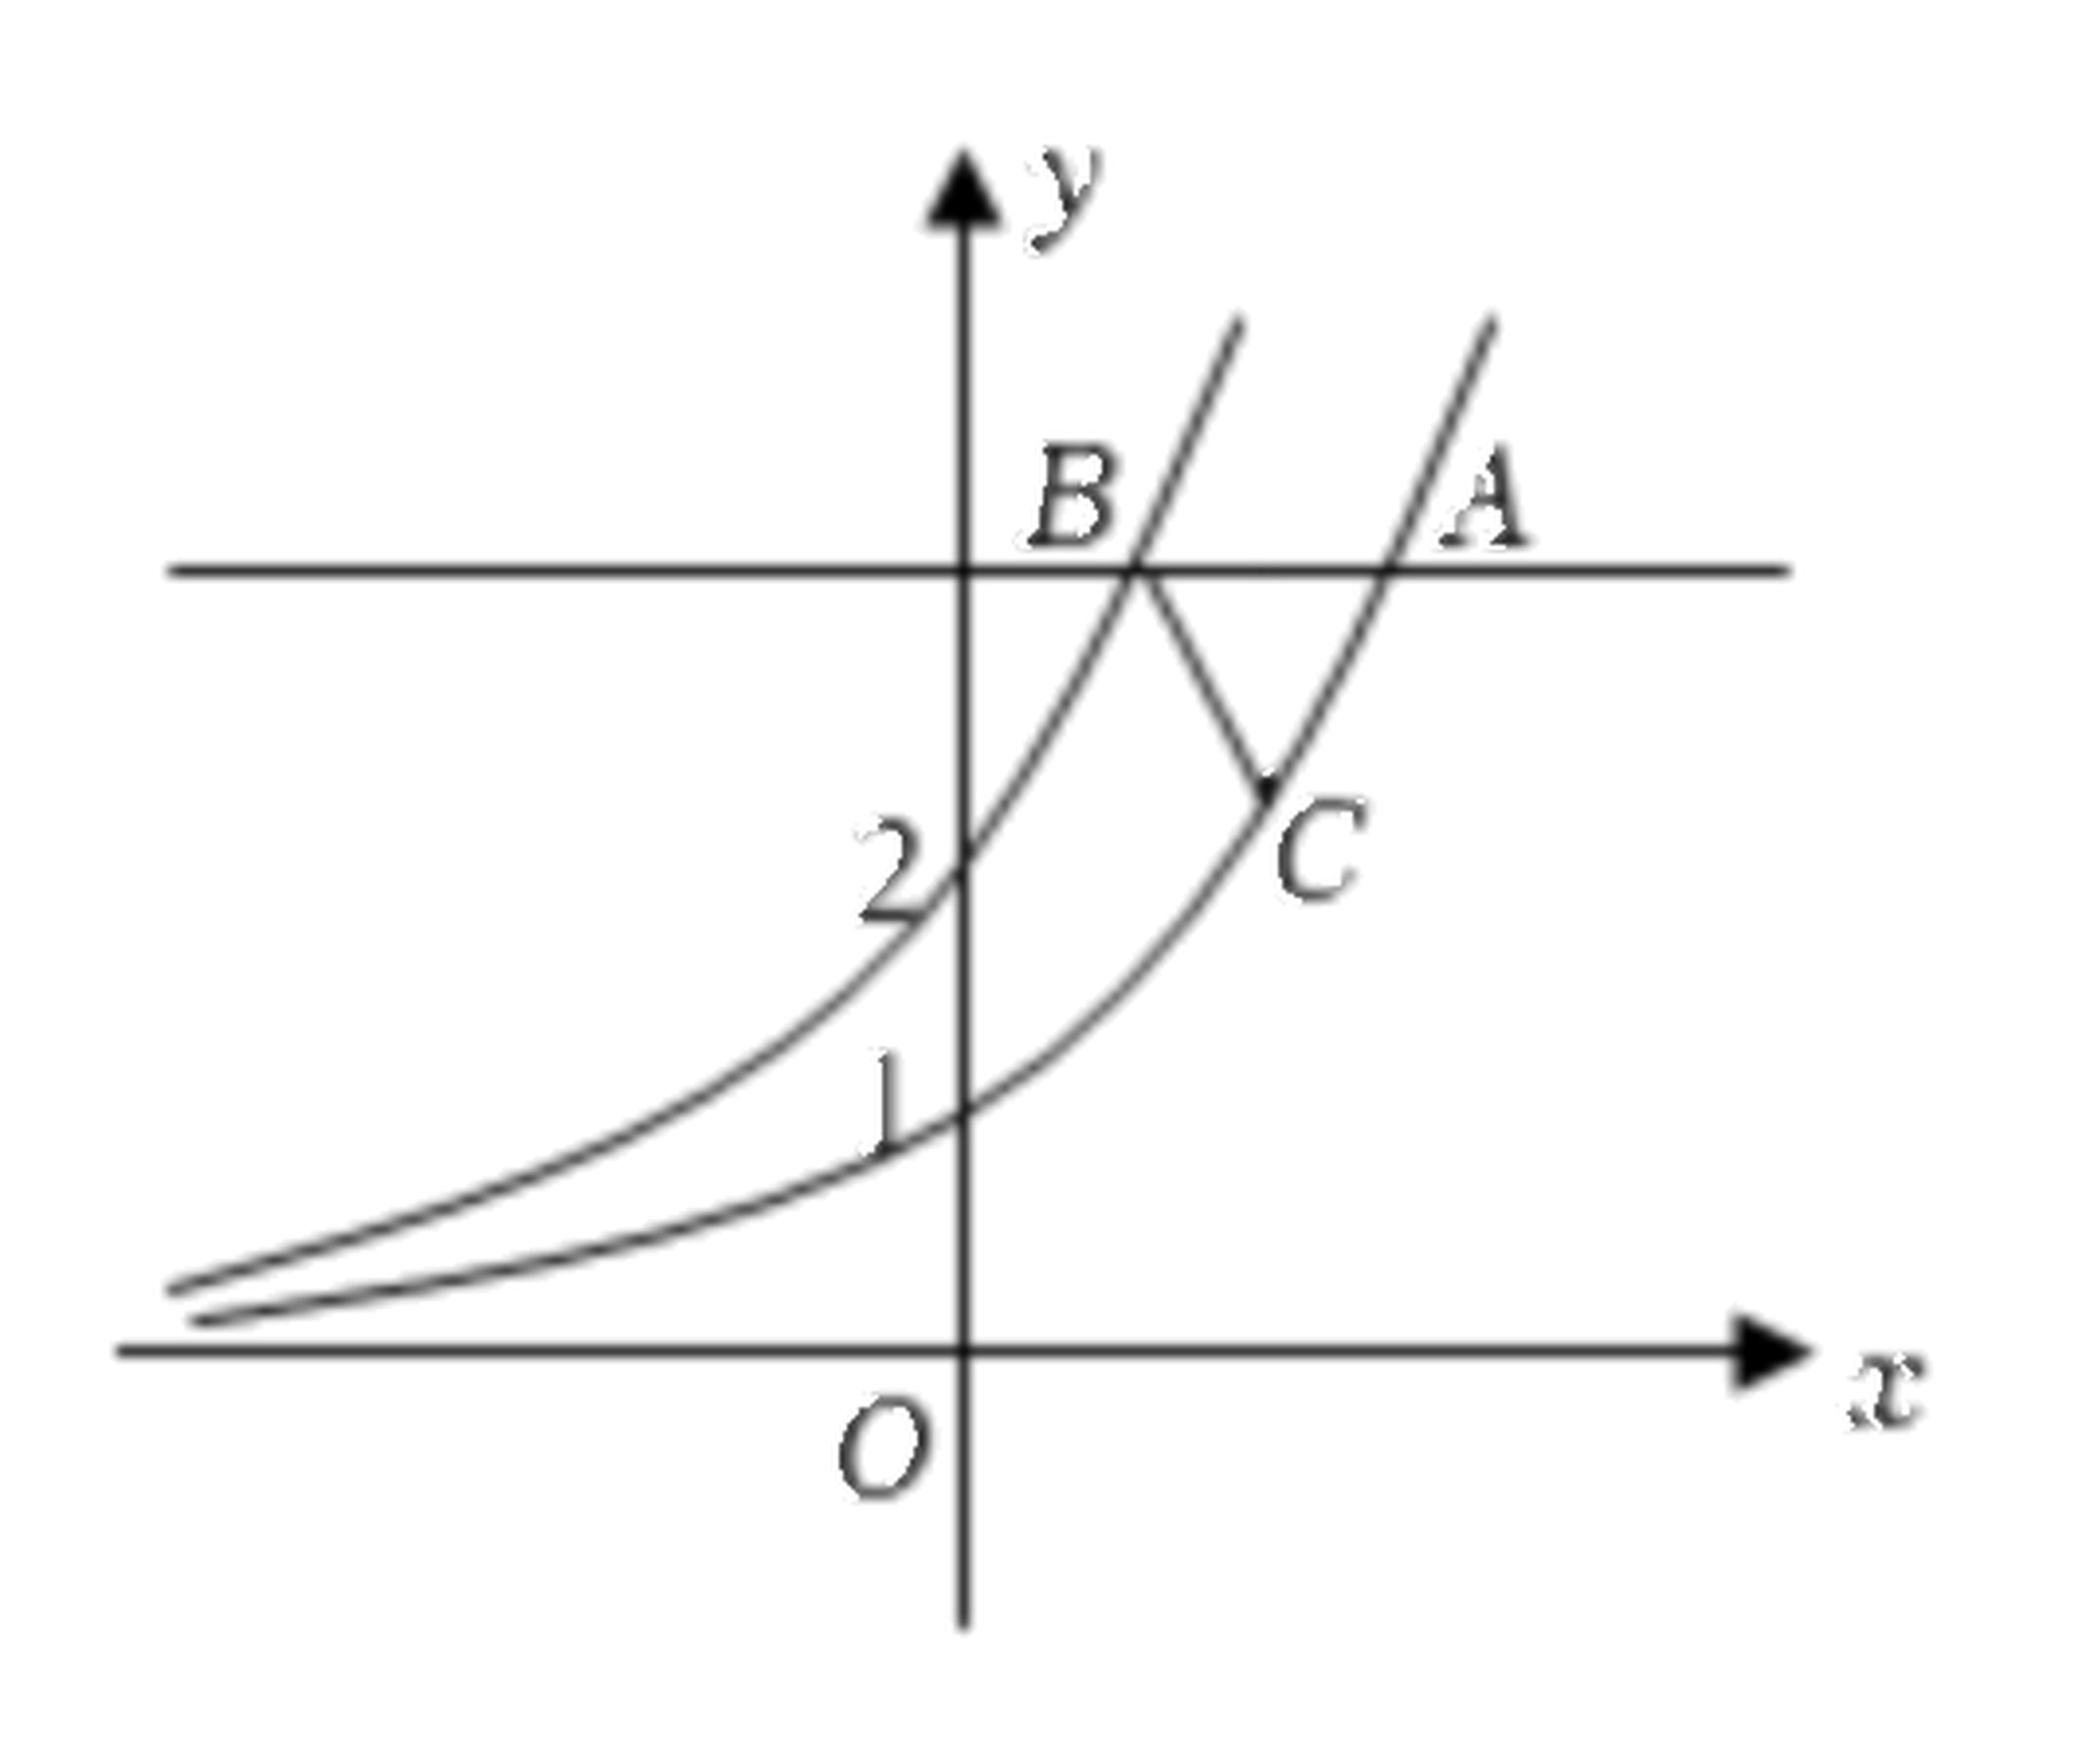
\includegraphics[width=0.40\textwidth]{figures/gao150_q11.png}
\end{center}

\ifanswer
\solbegin
\step{设直线 $l$ 的方程为 $y=a(a>0)$，}
\step{由 $2^x=a$，得 $x=\log_2 a$，所以 $A(\log_2 a,a)$，}
\step{由 $2^{x+1}=a$，得 $x=\log_2 a-1$，所以 $B(\log_2 a-1,a)$，所以 $\lvert AB\rvert=1$，}
\step{取 $AB$ 的中点 $D$，连接 $CD$，如图所示，}
\step{因为 $\triangle ABC$ 为等边三角形，则 $CD\perp AB$，且 $\lvert CD\rvert=\dfrac{\sqrt3}{2}$，}
\step{所以 $C\left(\log_2 a-\dfrac{1}{2},a-\dfrac{\sqrt3}{2}\right)$，}
\step{因为点 $C$ 在函数 $y=2^x$ 的图像上，所以 $a-\dfrac{\sqrt3}{2}=2^{\log_2 a-\frac{1}{2}}=\dfrac{a}{\sqrt2}$，}
\step{解得 $a=\dfrac{\sqrt3}{2-\sqrt2}=\dfrac{\sqrt3(2+\sqrt2)}{4-2}=\sqrt3+\dfrac{\sqrt6}{2}$，}
\step{所以点 $C$ 的纵坐标为 $a-\dfrac{\sqrt3}{2}=\dfrac{\sqrt3+\sqrt6}{2}$.}
\solend
\fi

% === Q12 === 解析配图（高斯函数方格阴影，仅答案版出）；"数学王子"弯引号；cases 块整体算一个印刷行；解析 4 行
\item 小玲在研究数学发展史，特别崇拜近代数学奠基者之一、享有“数学王子”称号的德国数学家高斯. 为了纪念高斯，我们把取整函数 $y=[x]$ 称为高斯函数，其中 $[x]$ 表示不超过 $x$ 的最大整数，如 $[1.1]=1$，$[-1.1]=-2$，则点集 $P=\{(x,y)\mid [x]^2+[y]^2=1\}$ 所表示的平面区域的面积为\blankline[4.4em].

\ifanswer
\solbegin
\step{$[x]^2+[y]^2=1$ 由 $\begin{cases}[x]=0\\ {[y]=-1}\end{cases}$ 或 $\begin{cases}[x]=0\\ {[y]=1}\end{cases}$ 或 $\begin{cases}[x]=-1\\ {[y]=0}\end{cases}$ 或 $\begin{cases}[x]=1\\ {[y]=0}\end{cases}$ 四个平面区域组成，}
\step{即 $\begin{cases}0\leqslant x<1\\ -1\leqslant y<0\end{cases}$ 或 $\begin{cases}0\leqslant x<1\\ 1\leqslant y<2\end{cases}$ 或 $\begin{cases}-1\leqslant x<0\\ 0\leqslant y<1\end{cases}$ 或 $\begin{cases}1\leqslant x<2\\ 0\leqslant y<1\end{cases}$，}
\step{作出平面区域如图所示，平面区域由四个边长为 $1$ 的正方形组成，}
\begin{center}
% 高斯函数 [x]^2+[y]^2=1 方格阴影区域图取 04 页顶部，去粉色水印、去色、4× LANCZOS 放大；仅答案版出
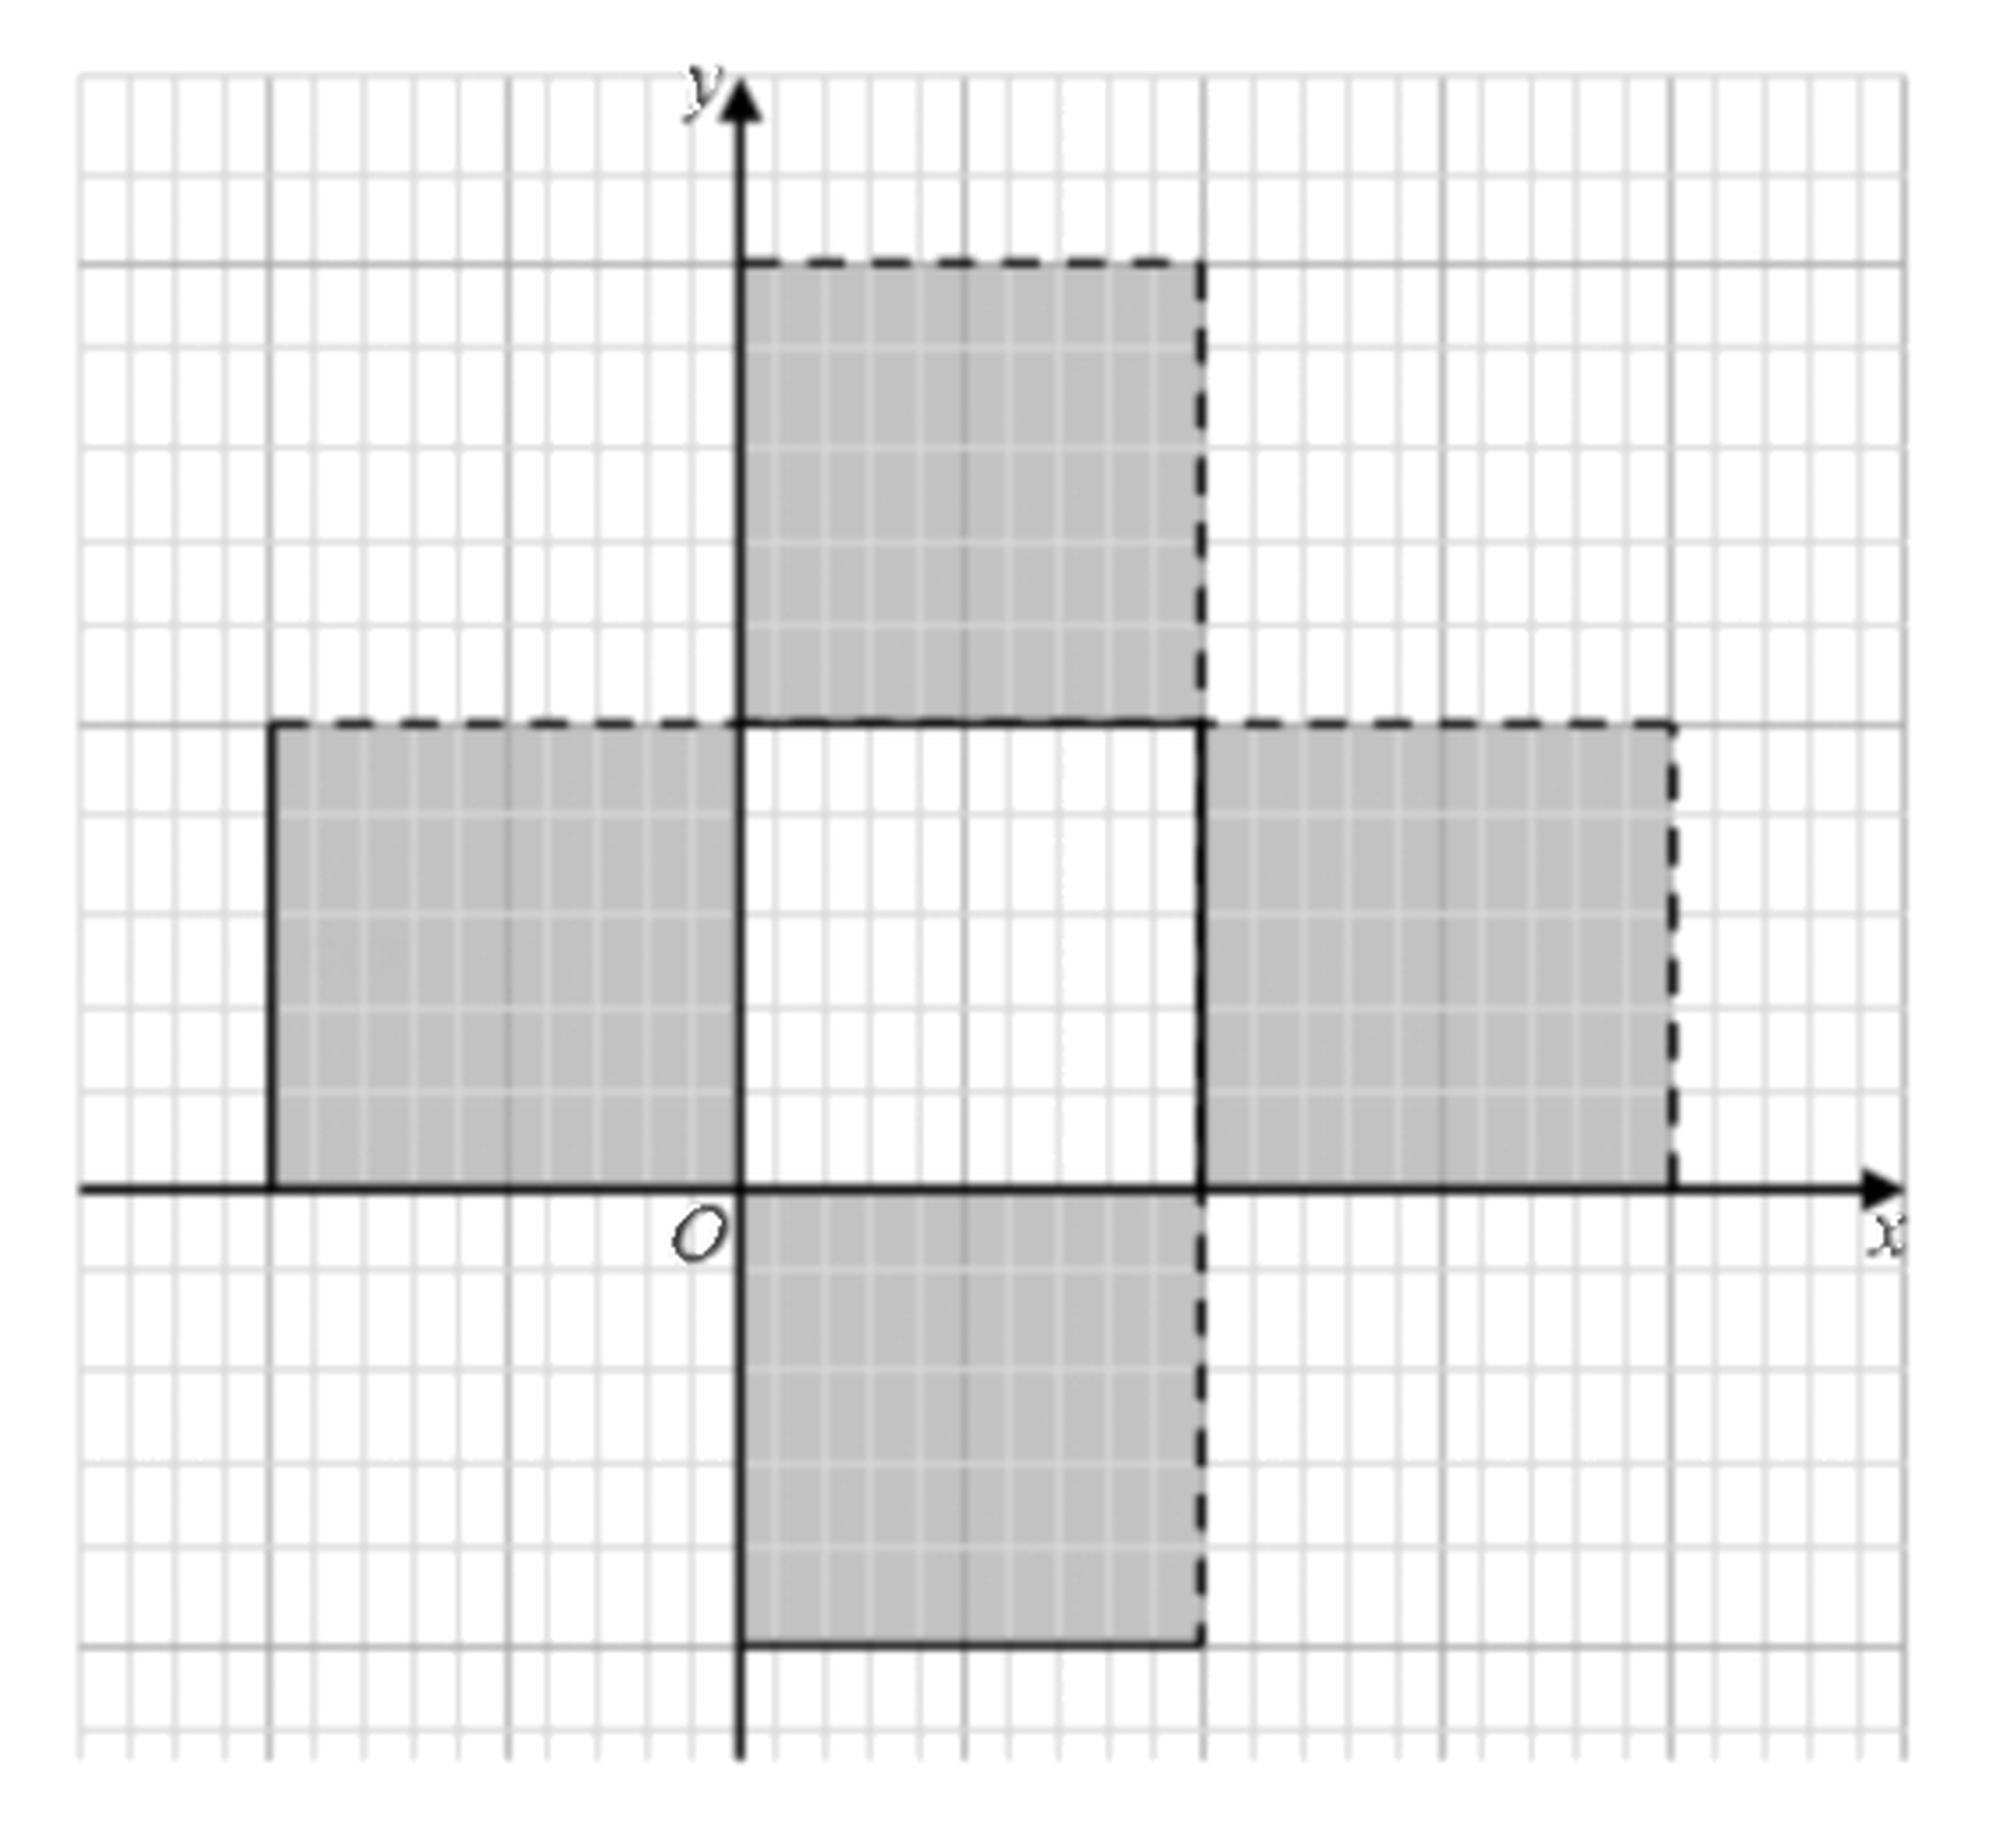
\includegraphics[width=0.34\textwidth]{figures/gao150_q12.png}
\end{center}
\step{总面积为 $1\times4=4$.}
\solend
\fi

\end{enumerate}

\bigsec{二、选择题}

\begin{enumerate}
\setcounter{enumi}{12}

% === Q13 === 答案在解析末句"故选 C"；括号 \mbox{（\quad）} 留空；四选项一行；解析 1 行
\item 设 $x\ne0$，则 $3^{\log_9 x^2}$ 的化简结果是\mbox{（\quad）}

\keepwithprev
A. $x$\qquad B. $\dfrac{1}{x}$\qquad C. $\lvert x\rvert$\qquad D. $\dfrac{1}{\lvert x\rvert}$

\ifanswer
\solbegin
\step{$3^{\log_9 x^2}=3^{\log_3\lvert x\rvert}=\lvert x\rvert$，故选 $C$.}
\solend
\fi

% === Q14 === 题目配图（两函数图像，三版都出）；\needvspace{8cm} 守卫放 \item 之前；"图像"照录；四选项两行两列；解析 2 行，故选 B
\needvspace{8cm}
\item 设 $a>0$ 且 $a\ne1$，$b\in\R$. 若函数 $y=a^{-\lvert x\rvert}$ 与 $y=x^b$ 的大致图像如图所示，则\mbox{（\quad）}

\keepwithprev
A. $0<a<1<b$\qquad\qquad B. $a>1$ 且 $b>1$

C. $0<a<1$ 且 $0<b<1$\qquad\qquad D. $0<b<1<a$

\begin{center}
% 两函数 y=a^{-|x|} 与 y=x^b 大致图像取 04 页右侧，去粉色水印、去色、4× LANCZOS 放大；三版都出
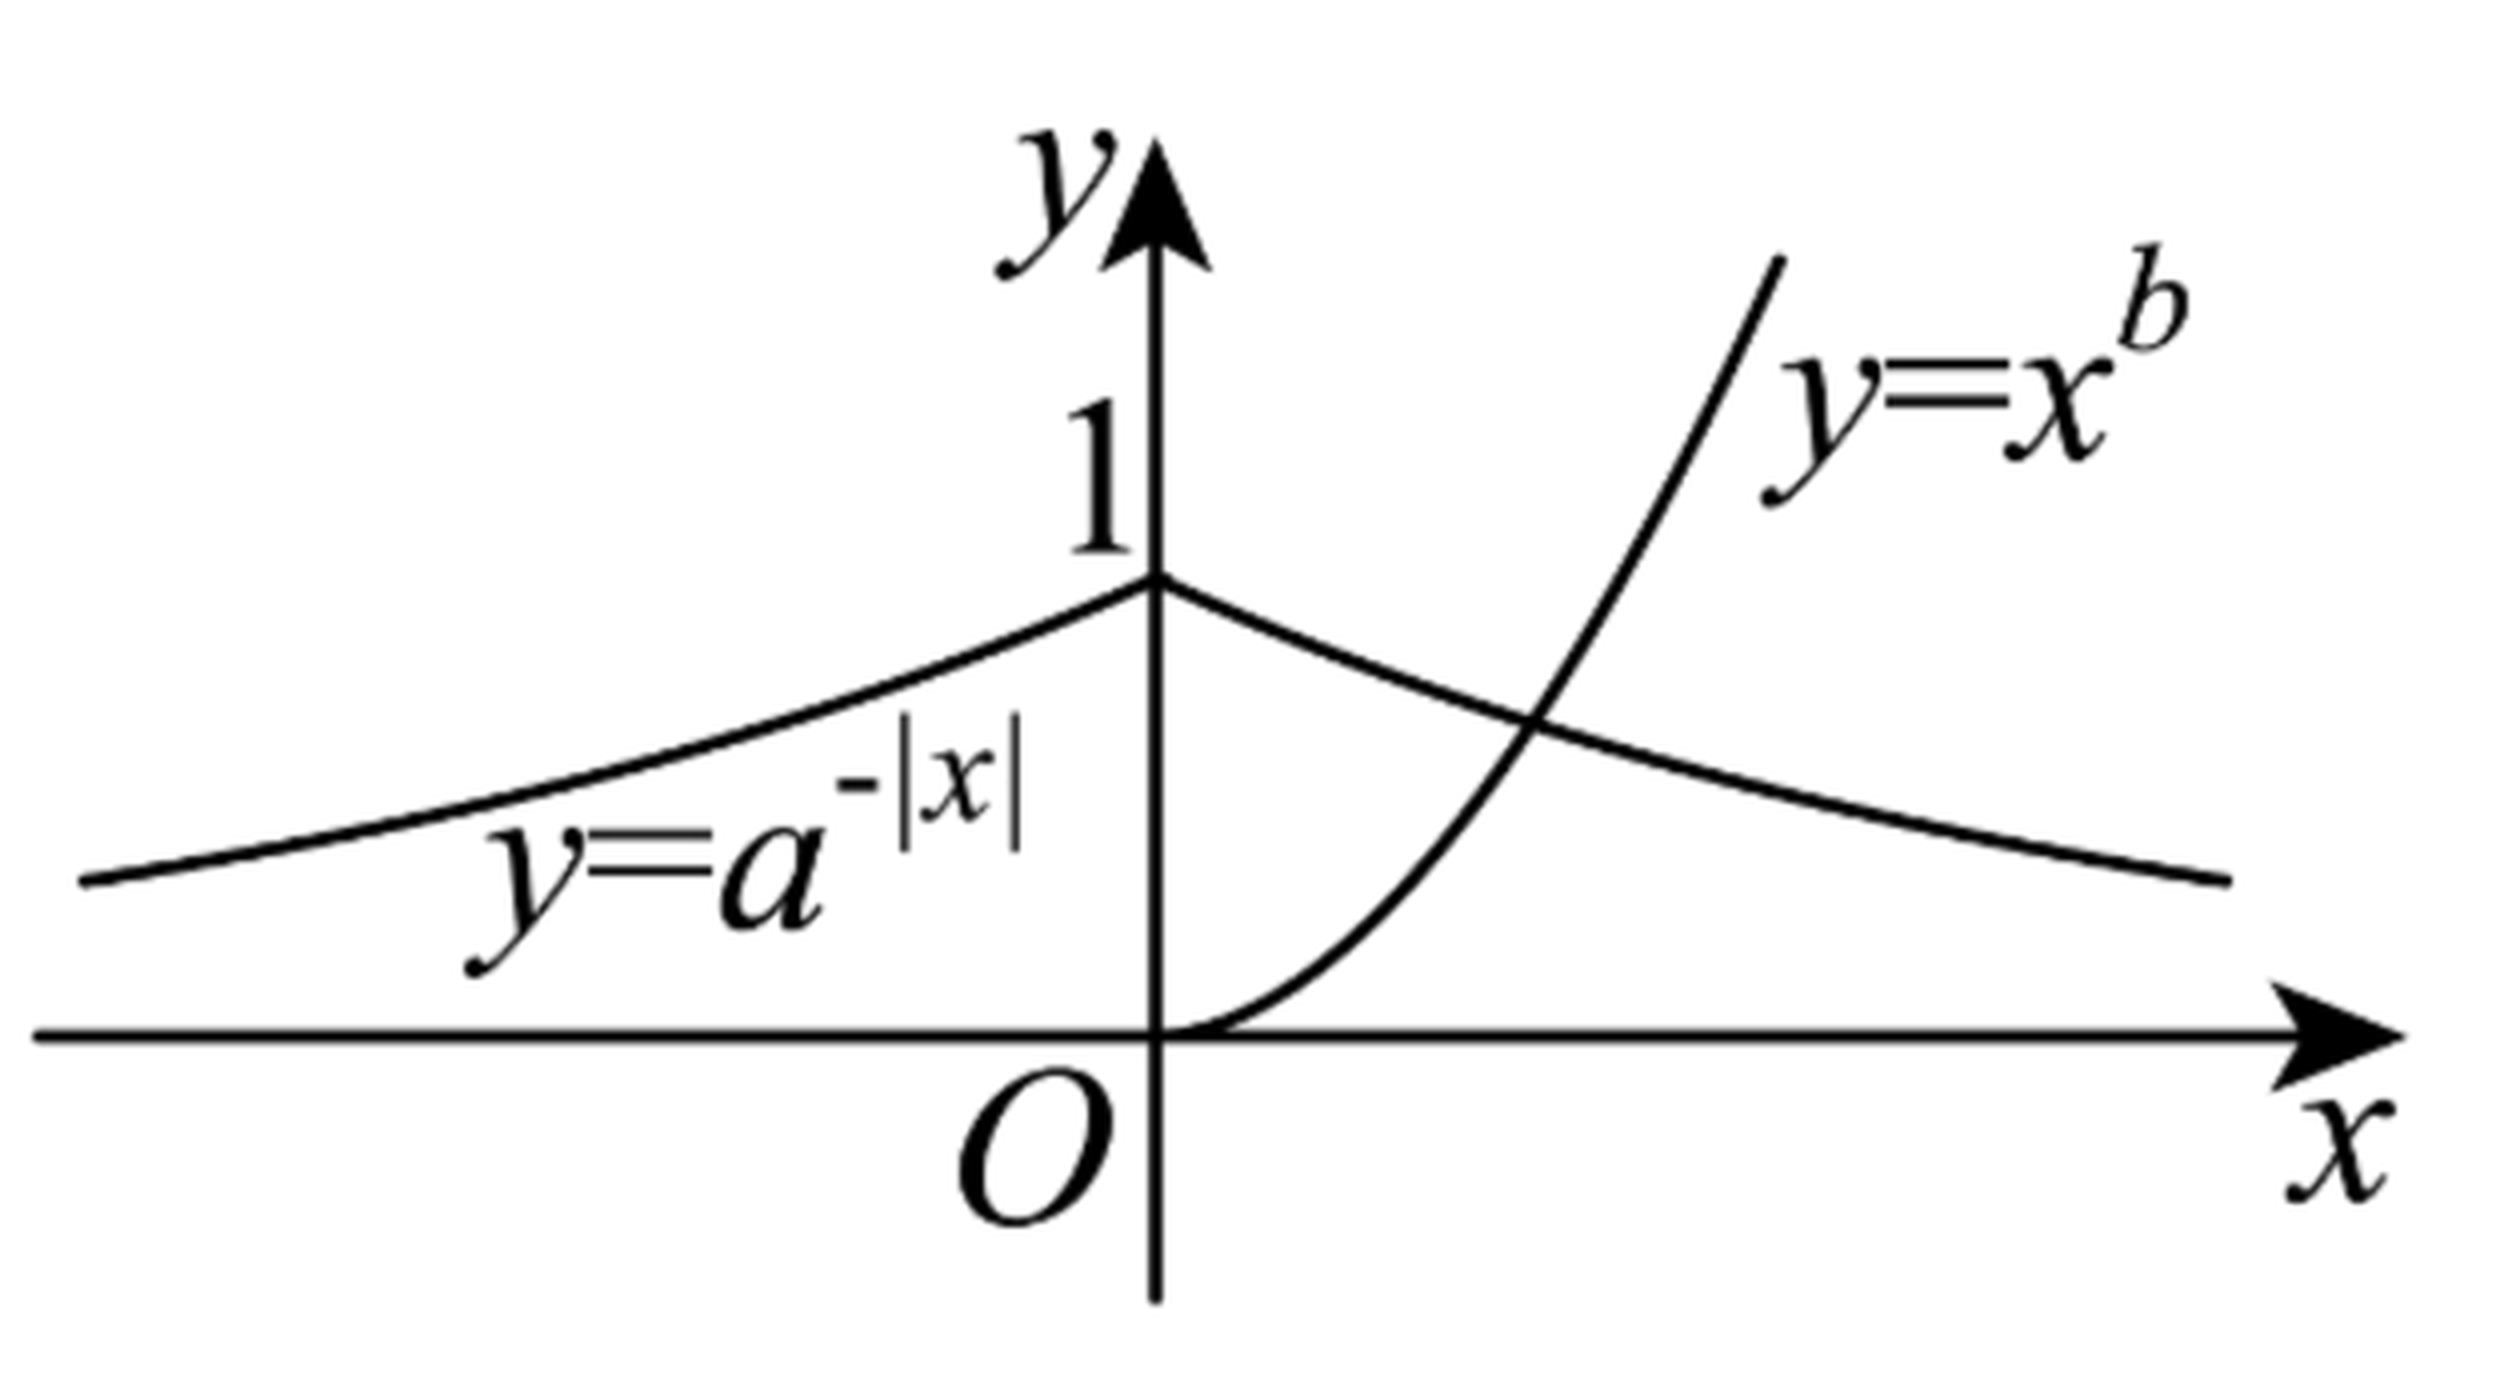
\includegraphics[width=0.40\textwidth]{figures/gao150_q14.png}
\end{center}

\ifanswer
\solbegin
\step{在 $(0,+\infty)$ 上，$y=a^{-x}$ 严格递减，得 $a>1$；}
\step{幂函数 $y=x^b$ 的图像递增且向上弯曲，得 $b>1$；故选 $B$.}
\solend
\fi

% === Q15 === "算术平均值／算术平均数"两处不同照录；四选项两行两列；解析 5 行（续 05 页顶），故选 B
\item 已知两个正数的算术平均值不小于它们的几何平均值，类比有以下结论：三个正数的算术平均数不小于它们的几何平均数，即当 $a,b,c$ 为正实数时，$\dfrac{a+b+c}{3}\geqslant\sqrt[3]{abc}$，当且仅当 $a=b=c$ 时等号成立. 利用上述结论，下列选项中判断正确的是\mbox{（\quad）}

\keepwithprev
A. 若 $x>0$，则 $2x+\dfrac{1}{x^2}\geqslant\dfrac{27}{8}$\qquad\qquad B. 若 $x>0$，则 $x^2+\dfrac{2}{x}\geqslant3$

C. 若 $0<x<1$，则 $x^2(1-x)\geqslant\dfrac{1}{9}$\qquad\qquad D. 若 $0<x<1$，则 $x^2(1-x)\leqslant\dfrac{1}{9}$

\ifanswer
\solbegin
\step{A：取 $x=1$，$2x+\dfrac{1}{x^2}=3<\dfrac{27}{8}$，错误.}
\step{B：$x^2+\dfrac{2}{x}=x^2+\dfrac{1}{x}+\dfrac{1}{x}\geqslant3\sqrt[3]{x^2\cdot\dfrac{1}{x}\cdot\dfrac{1}{x}}=3$，当且仅当 $x=1$ 时取等号，正确.}
\step{C：取 $x=\dfrac{1}{3}$，$x^2(1-x)=\dfrac{2}{27}<\dfrac{1}{9}$，错误.}
\step{D：取 $x=\dfrac{2}{3}$，$x^2(1-x)=\dfrac{4}{27}>\dfrac{1}{9}$，错误.}
\step{故选 $B$.}
\solend
\fi

% === Q16 === "完美集"新定义（弯引号、引号外空格照录）；圈数字①②文本模式；$n\in\N$；四选项两行两列；解析 9 行（6 行 05 页＋3 行 06 页顶），故选 A
\item 已知有限集 $A=\{a_1,a_2,\cdots,a_n\}$（$n\geqslant2$，$n\in\N$）. 若 $A$ 中元素 $a_i$（$i=1,2,\cdots,n$）满足 $a_1+a_2+\cdots+a_n=a_1\cdot a_2\cdots a_n$，就称 $A$ 为 “完美集”. 现有以下两个命题：

①恰有两个元素的 “完美集” 有无穷多个；

②若 $a_i$ 均为正整数，则 “完美集” $A$ 有且只有一个，且 $n=3$.

则\mbox{（\quad）}

\keepwithprev
A. ①和②都是真命题\qquad\qquad B. ①和②都是假命题

C. ①是真命题，②是假命题\qquad\qquad D. ①是假命题，②是真命题

\ifanswer
\solbegin
\step{①由 $a+b=ab\Leftrightarrow(a-1)(b-1)=1$，任取 $a>2$，则 $b=1+\dfrac{1}{a-1}\in(1,2)$，}
\step{得到无穷多个不同的完美集，①真.}
\step{②设 $1\leqslant a_1<a_2<\cdots<a_n$，则 $a_i\geqslant i$.}
\step{若 $n=2$，则 $(a_1-1)(a_2-1)=1$，只能有 $a_1=a_2=2$，与元素互异矛盾.}
\step{若 $n\geqslant4$，则 $a_1a_2\cdots a_n\geqslant a_2a_{n-1}a_n\geqslant2(n-1)a_n>na_n\geqslant a_1+\cdots+a_n$，矛盾.}
\step{当 $n=3$ 时，若 $a_1\geqslant2$，则 $a_1a_2a_3\geqslant6a_3>3a_3\geqslant a_1+a_2+a_3$，矛盾.}
\step{因此 $a_1=1$，$(a_2-1)(a_3-1)=2$，结合 $a_2<a_3$ 得 $a_2=2$，$a_3=3$.}
\step{唯一的完美集为 $\{1,2,3\}$，②真.}
\step{故选 $A$.}
\solend
\fi

\end{enumerate}

\bigsec{三、解答题}

\begin{enumerate}
\setcounter{enumi}{16}

% === Q17 === \varnothing 空集、$B\subseteq A$ 带下划线照录；弯引号内空格照录；解析 7 行
\item 设 $a,b\in\R$. 已知集合 $A=\{x\mid ax^2+3x-a>3\}$，$B=\{x\mid bx=1\}$.

(1) 若 $A=(1,2)$，求 $a$ 的值；

(2) 若 $a=0$，且 “ $x\in A$ ” 是 “ $x\in B$ ” 的必要非充分条件，求 $b$ 的取值范围.

\ifanswer
\solbegin
\step{(1) $A=(1,2)$，则 $a<0$，且 $1,2$ 是方程 $ax^2+3x-a-3=0$ 的两根.}
\step{由 $4a+6-a-3=0$，得 $a=-1$，此时不等式为 $-(x-1)(x-2)>0$，}
\step{解集确为 $(1,2)$.}
\step{(2) $a=0$ 时，$A=(1,+\infty)$，题意等价于 $B\subseteq A$ 且 $B\ne A$.}
\step{当 $b=0$ 时，$B=\varnothing$，符合条件.}
\step{当 $b\ne0$ 时，$B=\left\{\dfrac{1}{b}\right\}$，条件等价于 $\dfrac{1}{b}>1$，解得 $0<b<1$.}
\step{因此 $b$ 的取值范围为 $[0,1)$.}
\solend
\fi

% === Q18 === $p\in\Z$；"图像"（像，有亻）照录；指数 $-2p^2+5p$；解析 8 行（(1) 首行 06 页末＋2 行 07 页顶、(2) 5 行 07 页）
\item 设 $p\in\Z$，已知 $f(x)=x^{-2p^2+5p}$.

(1) 若幂函数 $y=f(x)$ 的图像关于原点成中心对称，且满足 $f(3)<f(4)$，求 $p$ 的值；

(2) 当 $p=-2$ 时，求满足 $f(2x+3)<f(x-4)$ 的 $x$ 的取值范围.

\ifanswer
\solbegin
\step{(1) 图像关于原点成中心对称，得整数 $-2p^2+5p$ 为奇数.}
\step{由 $f(3)<f(4)$，得 $-2p^2+5p>0\Leftrightarrow0<p<\dfrac{5}{2}$，}
\step{结合 $p\in\Z$，得 $p=1$ 或 $p=2$，对应指数分别为 $3$、$2$，所以 $p=1$.}
\step{(2) 当 $p=-2$ 时，$f(x)=\dfrac{1}{x^{18}}$，定义域为 $\{x\in\R\mid x\ne0\}$.}
\step{原不等式要求 $x\ne-\dfrac{3}{2}$ 且 $x\ne4$，}
\step{此时 $\dfrac{1}{(2x+3)^{18}}<\dfrac{1}{(x-4)^{18}}\Leftrightarrow\lvert 2x+3\rvert>\lvert x-4\rvert\Leftrightarrow(2x+3)^2>(x-4)^2$，}
\step{因此 $(x+7)(3x-1)>0\Leftrightarrow x<-7$ 或 $x>\dfrac{1}{3}$，}
\step{排除 $x=4$，得 $x\in(-\infty,-7)\cup\left(\dfrac{1}{3},4\right)\cup(4,+\infty)$.}
\solend
\fi

% === Q19 === $a\in\R$、$g(x)=f(2x+1)+a\cdot f(x)+2$；解析 6 行（(2) 末两行续 08 页顶）
\item 已知 $f(x)=2^x$.

(1) 求方程 $f(2x)-f(x)=6$ 的解；

(2) 设 $a\in\R$，$g(x)=f(2x+1)+a\cdot f(x)+2$，若对于任意 $x\in[-1,1]$，均有 $g(x)\geqslant1$，求 $a$ 的取值范围.

\ifanswer
\solbegin
\step{(1) 令 $t=2^x>0$，则 $t^2-t-6=(t-3)(t+2)=0$，}
\step{由 $t>0$ 得 $t=3$，所以 $x=\log_2 3$.}
\step{(2) 令 $t=2^x$，则 $t\in\left[\dfrac{1}{2},2\right]$，且 $g(x)\geqslant1\Leftrightarrow2t^2+at+1\geqslant0\Leftrightarrow a\geqslant-\left(2t+\dfrac{1}{t}\right)$，}
\step{由基本不等式得 $2t+\dfrac{1}{t}\geqslant2\sqrt{2t\cdot\dfrac{1}{t}}=2\sqrt2$，}
\step{当且仅当 $t=\dfrac{1}{\sqrt2}\in\left[\dfrac{1}{2},2\right]$ 时等号成立，}
\step{因此 $-\left(2t+\dfrac{1}{t}\right)$ 的最大值为 $-2\sqrt2$，所求范围为 $a\in[-2\sqrt2,+\infty)$.}
\solend
\fi

% === Q20 === "极闭集"新定义、3 问，全卷末题；$M\subseteq(0,+\infty)$ 带下划线照录；自定义运算 $x*y$ 星号照录；解析 13 行（9 行 08 页＋4 行 09 页上半）
\item 对于非空实数集 $M\subseteq(0,+\infty)$，若满足以下两个条件：

① $M$ 中至少含有 $2$ 个元素，且 $1\notin M$；

②对于 $M$ 中任意两个不相等的元素 $x$、$y$，定义 $x*y=\dfrac{xy+1}{x+y}$，且 $x*y\in M$.

则称 $M$ 为 “极闭集”.

(1) 分别判断集合 $A=\left\{\dfrac{1}{2},3\right\}$ 与集合 $B=(1,+\infty)$ 是否为 “极闭集” （无需理由）；

(2) 若 $M$ 是 “极闭集”，证明：$M$ 中不可能所有元素都小于 $1$；

(3) 证明：不存在任何有限集是 “极闭集”.

\ifanswer
\solbegin
\step{(1) $A$ 不是 “极闭集”，$B$ 是 “极闭集”.}
\step{(2) 假设 $M$ 中所有元素都小于 $1$，取其中两个不相等的元素 $x$、$y$，}
\step{则 $x*y-1=\dfrac{(1-x)(1-y)}{x+y}>0$，}
\step{这与 $x*y\in M$ 且 $M$ 中所有元素都小于 $1$ 矛盾.}
\step{(3) 假设有限集 $M$ 是 “极闭集”，}
\step{由 (2) 及 $1\notin M$，得 $M$ 中存在大于 $1$ 的元素.}
\step{若 $M$ 中有小于 $1$ 的元素，取其中最大的一个为 $a$，另取 $b\in M$ 且 $b>1$，}
\step{则 $a*b-a=\dfrac{1-a^2}{a+b}>0, a*b-1=\dfrac{(a-1)(b-1)}{a+b}<0$，}% 半角逗号在两个数学式组之间，全稿惯例、非笔误，照录
\step{于是 $a<a*b<1$ 且 $a*b\in M$，与 $a$ 的最大性矛盾.}
\step{若 $M$ 中没有小于 $1$ 的元素，则 $M\subseteq(1,+\infty)$.}
\step{取 $a=\min M$，另取 $b\in M$ 且 $b\ne a$，则 $a*b-a=\dfrac{1-a^2}{a+b}<0$，}
\step{于是 $a*b<a$ 且 $a*b\in M$，与 $a$ 的最小性矛盾.}
\step{因此不存在任何有限集是 “极闭集”.}
\solend
\fi

\end{enumerate}

\end{document}
"
%
% ① 原始材料：微信公众号"魔都数学加油站"文章，连载"27学年高一150"，原文标题
% "27学年高一150——2026-2027年上海市曹杨二中高一上期中"；
% 原文链接：https://mp.weixin.qq.com/s/xlQxmik8TZXR87RC6MnCrw 。
% 正文为 9 张 PNG 页（01/02/04/06/07/09 为 2560×3620，03/05/08 为 4762×6735，
% 同一篇各页分辨率混排，逐页按各自分辨率裁图核对，别按预览比例换算裁框）。
% 体例：讲评版——全 18 题均印【解析】（逐题核实，见 ② ②）。
% 题目、答案、解析均据原图转录；卷面粉红色/红色水印"魔都数学加油站"及公众号页脚未录入。
% 全卷插图清单（逐页通读 9 页确认）：3 幅——
%   · Q11 题目配图（指数函数曲线图，02 页右侧：x/y 轴、O、y=2^x 与 y=2^{x+1}
%     两曲线、A/B/C 三点、刻度 1/2、等边三角形 ABC），三版都出，裁 figures/gao150_q11.png；
%   · Q12 解析配图（高斯函数取整 [x]^2+[y]^2=1 方格阴影区域图，04 页顶部：4 个边长 1
%     的正方形组成的十字形阴影），解析"作出平面区域如图所示"处，仅答案版出，
%     放 \ifanswer 内 \step 之间，裁 figures/gao150_q12.png；
%   · Q14 题目配图（两函数 y=a^{-|x|} 与 y=x^b 大致图像，04 页右侧：x/y 轴、O、
%     y 轴刻度 1、一递减曲线一递增上翘曲线），三版都出，裁 figures/gao150_q14.png；
%   其余各页逐页确认无其它题目配图、无表格；Q11/Q12 解析"如图所示"对应的就是上列
%   已裁的图，不重复裁；09 页上半为 Q20(3) 解析续尾、下半仅水印、无正文。
%   3 图均取自原卷截图，去粉色水印、去色、4× LANCZOS 放大。
%
% 卷首标题：原卷印作"2026-2027 年曹杨二中高一上期中"，年份区间按全稿惯例排 en dash；
% 原卷卷面未印副标题，本稿按同期中卷知识模块口径补出"集合与常用逻辑用语、不等式、函数"。
%
% 题号体例（逐页核实定稿）：本卷共 18 题——一、填空题 3—12（10 题）、
% 二、选择题 13—16（4 题）、三、解答题 17—20（4 题）。
% 三节分别 \setcounter{enumi}{2}／{12}／{16}。原卷从第 3 题起、无第 1、2 题，
% 本稿保留原题号；全卷末题为第 20 题（"极闭集"新定义、3 问），无 Q21、无附加题节。
%
% ② 与原卷的排版差异：
%   ① 原文从第 3 题起，本稿保留原题号；共 18 题三节，解答题只有 4 题到 20；
%   ② 全 18 题均印【解析】，用 \solbegin…\solend；逐题核实无只印【答案】或
%      答案印题干括号内的题；四道选择题答案在解析末句"故选 X"（Q13 选 C、
%      Q14 选 B、Q15 选 B、Q16 选 A，逐个放大复核）、括号 \mbox{（\quad）} 留空、
%      不另提 \ans{}；答案版【答案】/【解析】标记数 = 18 = 全卷题数；
%   ③ 原卷卷面未印副标题，本稿按知识模块口径补出；
%   ④ 原卷填空横线按全稿惯例排 \blankline[4.4em]；选择题括号排 \mbox{（\quad）}、
%      选项段前按惯例加 \keepwithprev；解答题不留作答区、不加 \anspace（原卷为讲评版）；
%   ⑤ 数集黑板粗体：Q4"m\in R"、Q5"a,b\in R"、Q6"a,b,c\in R"、Q7"a\in R"、
%      Q10"a\in R"、Q14"b\in R"、Q17"a,b\in R"、Q18"p\in Z"／定义域"x\in R"、
%      Q19"a\in R"、Q16"n\in N" 原卷印斜体 R/Z/N，按全稿惯例归一 \R／\Z／\N；
%      绝对值排 \lvert…\rvert（Q7 |x+4|+|x-3|、Q11 |AB|／|CD|、Q13 |x|、
%      Q18 |2x+3|／|x-4|），集合描述竖线排 \mid（Q3、Q12、Q17、Q18、Q20），
%      不等号按全稿惯例排 \leqslant／\geqslant；补集照原卷上划线排 \overline{A}
%      （Q3 题干＋解析共 2 处）；空集符号 \varnothing（Q17 解析(2)）；
%      子集 \subset（单线⊂）／\subseteq（带下划线⊆）逐处照录，本卷 3 处子集
%      符号均印带下划线 ⊆、照录 \subseteq（Q20 题干、Q20 解析(3)、Q17 解析(2)，
%      见 ④），无 \subset 用例；
%   ⑥ 判别式 Δ/△：逐页通读 9 页，本卷无一元二次判别式算式，故无 Δ/△ 混用可照录
%      （"高 \Delta／扁 \triangle"口径备查，参照 高一142／144／145／146／148／149
%      头注④）；本卷仅 Q11 题干与解析共 2 处几何三角形符号 △ABC，逐处放大并排
%      确认两处同形、印近等边粗线三角（非判别式），照录 \triangle（见 ④）；
%   ⑦ 中文弯引号照录：Q12"数学王子"、Q16"完美集"（题干＋①②两命题，引号外
%      留空格）、Q17" x∈A "" x∈B "（引号内空格）、Q20"极闭集"（题干条件、
%      三问与解析，引号外留空格）；注释里一律 ASCII 引号；数学式内 CJK 用 \text{}
%      （Q3 集合描述"且"用 \text{ 且 }）；
%   ⑧ 半角逗号在数学组之间是全稿惯例、非笔误，逐处照录（Q17 解析"1,2 是方程…
%      两根"、Q20 解析(3)">0, a*b-1=…<0" 两式之间等）；行末西文句点 ASCII `.`；
%      行中全角逗号／顿号照录（Q12"之一、享有"、Q18 解析"3、2"、Q20"x、y"）；
%   ⑨ "图像／图象"逐处放大核：全卷 9 处均印"图像"（像，有亻）、未见"图象"——
%      Q4 题干 1、Q11 题干 2＋解析 1、Q14 题干 1＋解析 1、Q18 题干 1＋解析 1；
%      同卷"第二象限""象限"用"象"（无亻）。逐处照录未统一改动（放大 01/02/04/06
%      页 /tmp/gao150/z/p01_q4_tuxiang2.png、p04_q14_tuxiang2.png、
%      p02_q11_lines.png 确认）；子题标号 (1)(2)(3) 半角括号照录；圈数字①②
%      在文本模式（Q16 两命题与解析、Q20 两条件与三问及解析）按 common.sty
%      划入 CJK 字符类渲染，进数学式用 \text{①}；
%   ⑩ Q20 新定义 x*y=\dfrac{xy+1}{x+y} 的 * 是自定义运算（星号），照录；
%      \left…\right 不得拆到不同 $…$ 组（Q19"\left(2t+\frac1t\right)"、
%      Q20 题干"A=\left\{\frac12,3\right\}"等）；Q8 嵌套根号
%      \sqrt{\frac2x+\frac{16}{1-2x}}、Q9 对数连加 \log_2 A 等复杂式照录别简化；
%   ⑪ 一条 \step = 原卷解析的一个印刷行，cases 块整体算一个印刷行；别并折行、
%      别拆行。Q4 三行、Q8 五行、Q11 九行、Q12 四行（两行各含四个 cases 块）、
%      Q15 五行、Q16 九行、Q18 八行、Q20 十三行均按印刷行逐条断，不丢行；
%   ⑫ 配图：Q11／Q14 题目配图（三版都出）放 \item 内题干之后 \begin{center}，
%      大图块加 \needvspace{8cm} 守卫把整块推走（守卫放 \item 之前，见
%      高一145 Q14/Q20 成例与切页审计 B 类坑）；Q12 解析配图（仅答案版出）
%      放 \ifanswer 内 \solbegin…\solend 的 \step 之间（高一73 第16题成例）；
%   ⑬ 跨页续印按题合并：见 ⑥；
%   ⑭ 原卷解析内无红色"法一／法二"之类小标题，故本卷无 \stepm；红色水印
%      "魔都数学加油站"不录入；Q12 解析"作出平面区域如图所示"对应的图即
%      ① 所列 gao150_q12.png（04 页顶部），不重复裁；Q11 解析"如图所示"对应
%      题目配图 gao150_q11.png，不另裁。
%
% ③ 行数复核：一条 \step／\stepm = 原卷解析的一个印刷行，cases 块作一个印刷行计。
%   逐题数（主会话逐页核对定稿）：Q3：1；Q4：3；Q5：2；Q6：1；Q7：2；Q8：5；
%   Q9：1；Q10：3；Q11：9；Q12：4；Q13：1；Q14：2；Q15：5；Q16：9；
%   Q17：7；Q18：8；Q19：6；Q20：13。
%   合计 82 条 \step（本卷无 \stepm：解析内无红色"法一／法二"类小标题），
%   与原卷逐题印刷行相等。全卷 18 题均设 \solbegin…\solend，答案版
%   【答案】/【解析】标记数 = 18 = 全卷题数。
%
% ④ 判别式／三角形／子集符号结论（逐处放大原图照录、不得统一，主会话像素级复核）：
%   判别式：逐页通读 9 页，本卷无一元二次判别式 Δ/△ 算式（Q18 讨论幂函数指数
%     奇偶、不用判别式；Q9／Q19／Q20 亦无），头注 ② ⑥ 的"高 \Delta／扁 \triangle"
%     口径在本卷无对应处（参照 高一142／144／145／146／148／149 头注④，仅备查）。
%   几何三角形符号：Q11 题干"使得 △ABC 为等边三角形"（02 页末）与解析
%     "因为 △ABC 为等边三角形，则 CD⊥AB"（03 页）共 2 处，放大 02/03 页
%     /tmp/gao150/z/q11_tri_montage2.png 并排确认两处同形、印近等边粗线三角
%     （h/w≈0.98、非"高>宽"的判别式 \Delta），照录 \triangle（与 高一105
%     "使得 \triangle ABC 为等边三角形" 同短语成例、高一149 几何三角形照录
%     \triangle 口径一致），不引入 \Delta。
%   子集／补集：Q20 题干"$M\subseteq(0,+\infty)$"（08 页）、Q20 解析(3)
%     "则 $M\subseteq(1,+\infty)$"（09 页）、Q17 解析(2)"题意等价于 $B\subseteq A$
%     且 $B\ne A$"（06 页）共 3 处子集符号，逐处放大（/tmp/gao150/z/p08_q20_stem.png、
%     p09_q20_sub.png、p06_q17_sub.png）确认均印带下划线 ⊆，照录 \subseteq；
%     本卷未见单线 ⊂（\subset）之对应处。Q3 题干与解析共 2 处补集照原卷上划线
%     排 \overline{A}；Q17 解析(2) 空集印 ∅、照录 \varnothing（Q7"解集为空集"
%     为中文词、非符号，照录文字）；集合描述竖线 \mid；数集 \R／\Z／\N 归一见 ② ⑤。
%
% ⑤ 存疑照录（放大原图确认，照录未改、正文对应处另有 % 注）：
%   1. Q8 解析第 4 行"所以 $y=\frac1x+\frac{8}{1-2x}$ 的最小值为 18" —— 上文
%      并未定义 $y$，且题面求的是 $\sqrt{\frac2x+\frac{16}{1-2x}}$ 的最小值；
%      按上下文该行应为 $\frac1x+\frac{8}{1-2x}$ 的最小值为 18（$y$ 疑为原卷
%      衍字／笔误），放大 02 页 /tmp/gao150/z/p02_q8_y.png 确认，照录未改。
%   2. Q20 解析(3)"$a*b-a=\frac{1-a^2}{a+b}>0, a*b-1=\frac{(a-1)(b-1)}{a+b}<0$"
%      两式之间的逗号原卷印半角 ,（非全角），按全稿惯例"半角逗号在数学组之间"
%      照录未改（放大 08 页 /tmp/gao150/z/p08_q20_sol8.png 确认）。
%   3. Q15 题干"两个正数的算术平均值…几何平均值"与"三个正数的算术平均数…
%      几何平均数"两处"值／数"用字不同，逐处照录未统一（放大 04 页确认）。
%   4. "图像／图象"全卷 9 处均印"图像"（像，有亻）、未见"图象"，逐处放大核实
%      照录、未统一改动（见 ② ⑨）；本卷判别式 Δ/△ 无用例、几何三角形 2 处
%      照录 \triangle（见 ④）。
%   全卷除此 4 类外未发现其它笔误／自相矛盾处；18 题均印【解析】、无只印【答案】
%   或答案印题干括号内的题（见 ② ②）。
%
% ⑥ 跨页续印按题合并说明（逐页核实定稿）：Q3/4/5/6/7 题干＋解析在 01 页；
%   Q8 题干＋解析 5 行、Q9 题干＋解析 1 行在 02 页上半；Q10 题干＋解析 3 行
%   在 02 页下半；Q11 题干（前两行）＋配图在 02 页下半、题干续"三角形，则点 C
%   的纵坐标为___"与解析 9 行全在 03 页上半（解析"如图所示"对应题目配图）；
%   Q12 题干＋解析 4 行在 03 页下半，解析配图（方格阴影）续印在 04 页顶部；
%   "二、选择题"标题在 04 页中部；Q13 题干＋选项＋解析、Q14 题干＋选项＋
%   配图＋解析在 04 页；Q15 题干＋四选项在 04 页末、解析 5 行续 05 页上半；
%   Q16 题干＋①②两命题＋"则(  )"＋四选项＋解析前 6 行在 05 页、解析末 3 行
%   （"因此 a_1=1…②真""故选 A"）续 06 页顶部；"三、解答题"标题在 06 页；
%   Q17 题干(1)(2)＋解析(1) 3 行＋解析(2) 首行在 06 页、解析(2) 续 3 行
%   在 06 页下半；Q18 题干(1)(2)＋解析(1) 首行在 06 页末、解析(1) 续 2 行＋
%   解析(2) 5 行在 07 页上半；Q19 题干(1)(2)＋解析(1) 2 行＋解析(2) 前 2 行
%   在 07 页下半、解析(2) 末 2 行续 08 页顶部；Q20 题干（新定义＋①②两条件）
%   ＋三问＋解析(1)(2)(3) 前 9 行在 08 页、解析(3) 末 4 行续 09 页上半，
%   末行"因此不存在任何有限集是极闭集"为全卷收尾（09 页下半仅水印、无正文）。
%   本稿按题连排，不丢行、不并折行；全卷末题为第 20 题，无 Q21、无附加题节。
%
\documentclass[a4paper,11pt]{article}
\usepackage{common}

\begin{document}

\examtitlest[3]{2026--2027 年曹杨二中高一上期中}{集合与常用逻辑用语、不等式、函数}

\bigsec{一、填空题}

\begin{enumerate}
\setcounter{enumi}{2}

% === Q3 === 补集上划线 \overline{A}（题干＋解析各 1 处）；集合描述竖线 \mid、数学式内"且"用 \text{}；解析 1 行
\item 设全集 $U=\{1,2,3,4,5\}$，集合 $A=\{x\mid x^2-3x\leqslant0\text{ 且 }x\in U\}$，则 $\overline{A}=$\blankline[4.4em].

\ifanswer
\solbegin
\step{$x^2-3x\leqslant0\Leftrightarrow0\leqslant x\leqslant3$，所以 $A=\{1,2,3\}$，$\overline{A}=\{4,5\}$.}
\solend
\fi

% === Q4 === "图像"（像，有亻）逐处照录、同句"第二象限"用"象"（无亻）；解析 3 行
\item 设 $m\in\R$. 若幂函数 $y=(m^2-5m+1)x^{m+1}$ 的图像经过第二象限，则 $m=$\blankline[4.4em].

\ifanswer
\solbegin
\step{幂函数的系数为 1，故 $m^2-5m+1=1\Rightarrow m=0$ 或 $m=5$.}
\step{$m=0$ 时，$y=x$ 不经过第二象限；}
\step{$m=5$ 时，$y=x^6$ 经过第二象限，因此 $m=5$.}
\solend
\fi

% === Q5 === 解析 2 行
\item 设 $a,b\in\R$. 若 $a^2+\dfrac{b^2}{4}=1$，则 $ab$ 的最大值为\blankline[4.4em].

\ifanswer
\solbegin
\step{$1-ab=\left(a-\dfrac{b}{2}\right)^2\geqslant0$，即 $ab\leqslant1$；}
\step{当 $a=\dfrac{\sqrt2}{2}$，$b=\sqrt2$ 时取等号，最大值为 1.}
\solend
\fi

% === Q6 === 解析 1 行
\item 设 $a,b,c\in\R$. 若等式 $2x^2-3x-2=a(x-1)^2+b(x-1)+c$ 恒成立，则 $a-b+c=$\blankline[4.4em].

\ifanswer
\solbegin
\step{令 $x=0$，得 $a-b+c=-2$.}
\solend
\fi

% === Q7 === 绝对值 \lvert…\rvert；解析 2 行
\item 设 $a\in\R$. 若关于 $x$ 的不等式 $\lvert x+4\rvert+\lvert x-3\rvert<a$ 的解集为空集，则 $a$ 的取值范围是\blankline[4.4em].

\ifanswer
\solbegin
\step{$\lvert x+4\rvert+\lvert x-3\rvert\geqslant\lvert(x+4)-(x-3)\rvert=7$，当 $-4\leqslant x\leqslant3$ 时取等号.}
\step{原不等式的解集为空集当且仅当 $a\leqslant7$，即 $a\in(-\infty,7]$.}
\solend
\fi

% === Q8 === 嵌套根号 \sqrt{\frac{2}{x}+\frac{16}{1-2x}} 照录别简化；解析 5 行
\item 设 $x\in\left(0,\dfrac{1}{2}\right)$，则 $\sqrt{\dfrac{2}{x}+\dfrac{16}{1-2x}}$ 的最小值为\blankline[4.4em].

\ifanswer
\solbegin
\step{因为 $x\in\left(0,\dfrac{1}{2}\right)$，所以 $1-2x>0$，又 $2x+1-2x=1$，}
\step{所以 $\left(\dfrac{1}{x}+\dfrac{8}{1-2x}\right)(2x+1-2x)=10+\dfrac{1-2x}{x}+\dfrac{16x}{1-2x}$}
\step{$\geqslant10+2\sqrt{\dfrac{1-2x}{x}\cdot\dfrac{16x}{1-2x}}=18$，}
\step{当且仅当 $\dfrac{1-2x}{x}=\dfrac{16x}{1-2x}$ 即 $x=\dfrac{1}{6}$ 时取等号，所以 $y=\dfrac{1}{x}+\dfrac{8}{1-2x}$ 的最小值为 18，}% 原卷此处径写 $y=\frac1x+\frac{8}{1-2x}$（上文未定义 $y$、且与题面根式不符），疑笔误，放大 02 页确认，照录未改（见 ⑤）
\step{所以 $\sqrt{\dfrac{2}{x}+\dfrac{16}{1-2x}}$ 的最小值为 6.}
\solend
\fi

% === Q9 === 对数连加 \log_2 A 等复杂式照录别简化；解析 1 行
\item 记 $A=1\times2\times3\times\cdots\times2026$，则 $\dfrac{1}{\log_2 A}+\dfrac{1}{\log_3 A}+\dfrac{1}{\log_4 A}+\cdots+\dfrac{1}{\log_{2026}A}=$\blankline[4.4em].

\ifanswer
\solbegin
\step{原式 $=\log_A 2+\cdots+\log_A 2026=\log_A(2\times3\times\cdots\times2026)=\log_A A=1$.}
\solend
\fi

% === Q10 === "严格减函数／不恒为负／⇔"照录；解析 3 行
\item 设 $a\in\R$，$f(x)=\dfrac{ax+1}{x+2}$. 若函数 $y=f(x)$ 在 $[1,+\infty)$ 上是严格减函数，且在 $[1,+\infty)$ 上的函数值不恒为负，则 $a$ 的取值范围是\blankline[4.4em].

\ifanswer
\solbegin
\step{当 $1\leqslant x_1<x_2$ 时，$f(x_2)-f(x_1)=\dfrac{(2a-1)(x_2-x_1)}{(x_1+2)(x_2+2)}$，故严格递减 $\Leftrightarrow a<\dfrac{1}{2}$.}
\step{此时最大函数值为 $f(1)$，函数值不恒为负 $\Leftrightarrow f(1)=\dfrac{a+1}{3}\geqslant0\Leftrightarrow a\geqslant-1$，}
\step{得 $a\in\left[-1,\dfrac{1}{2}\right)$.}
\solend
\fi

% === Q11 === 题目配图（指数函数曲线，三版都出）；\needvspace{8cm} 守卫放 \item 之前；"图像"照录、几何三角形 \triangle；解析 9 行（全在 03 页）
\needvspace{8cm}
\item 如图，点 $C$ 是函数 $y=2^x$ 的图像上的一点，若存在平行于 $x$ 轴的直线 $l$ 分别与函数 $y=2^x$ 和 $y=2^{x+1}$ 的图像相交于点 $A$、$B$，使得 $\triangle ABC$ 为等边三角形，则点 $C$ 的纵坐标为\blankline[4.4em].

\begin{center}
% 指数函数曲线图取 02 页右侧，去粉色水印、去色、4× LANCZOS 放大；三版都出
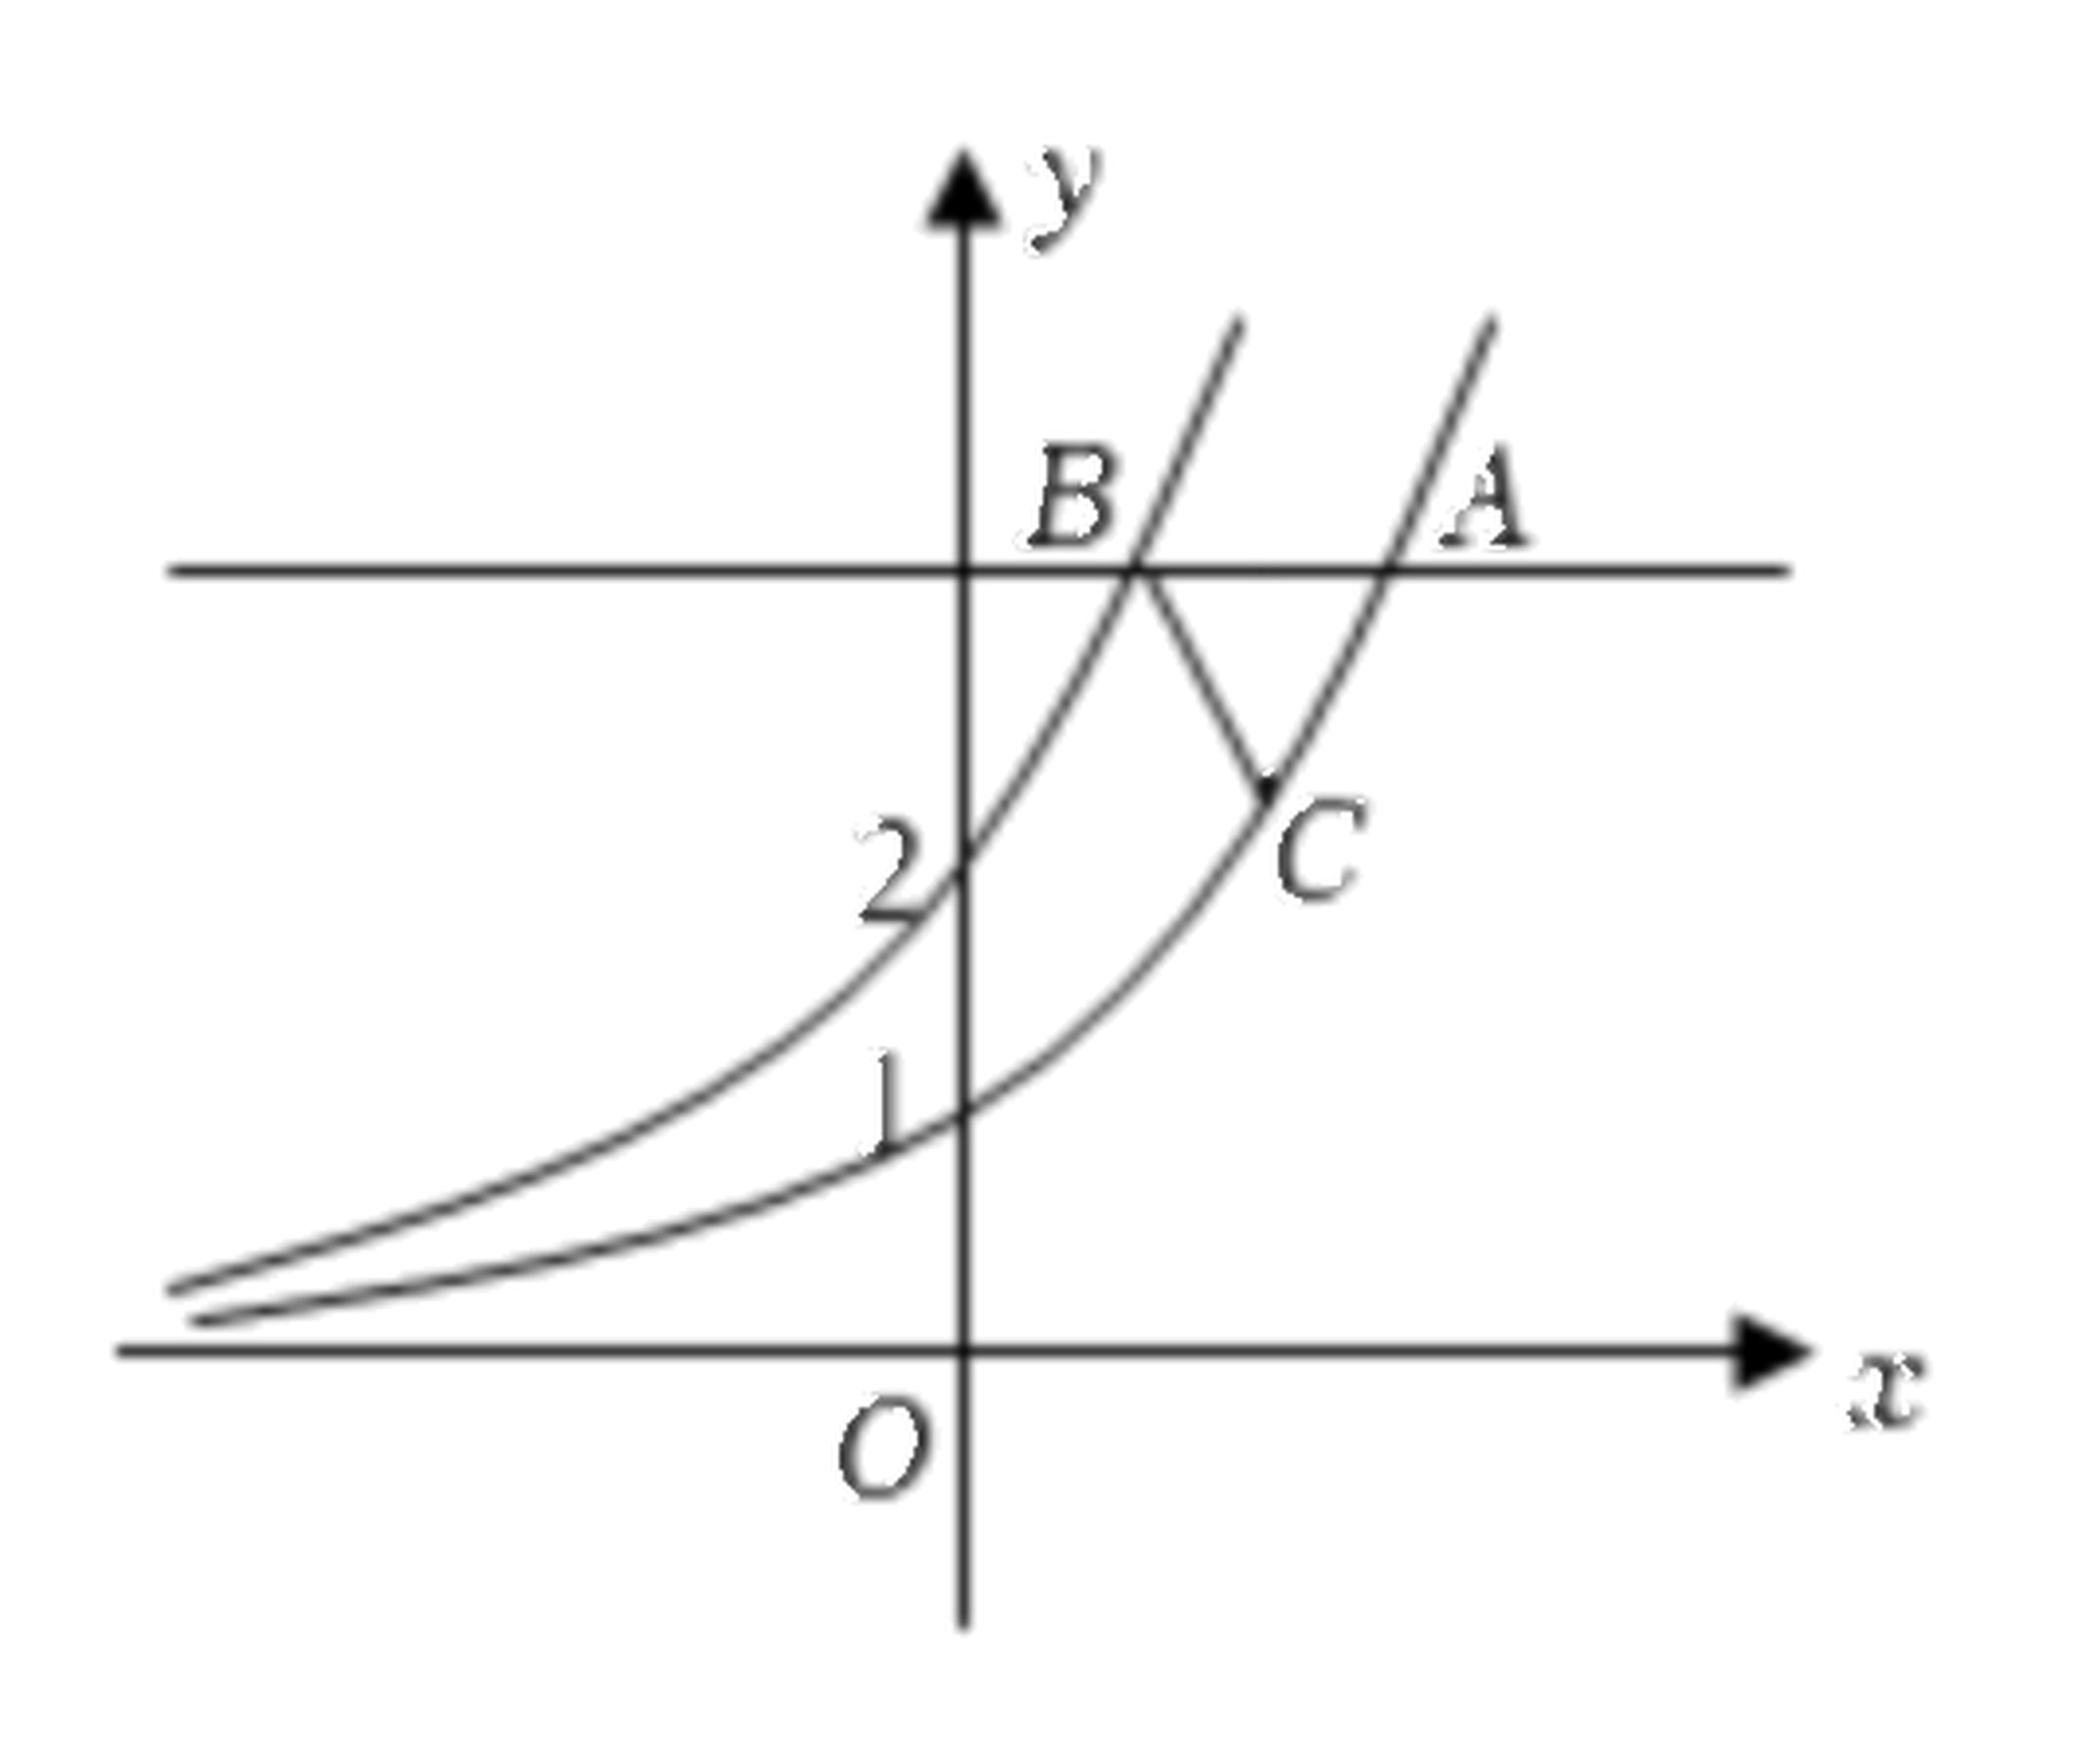
\includegraphics[width=0.40\textwidth]{figures/gao150_q11.png}
\end{center}

\ifanswer
\solbegin
\step{设直线 $l$ 的方程为 $y=a(a>0)$，}
\step{由 $2^x=a$，得 $x=\log_2 a$，所以 $A(\log_2 a,a)$，}
\step{由 $2^{x+1}=a$，得 $x=\log_2 a-1$，所以 $B(\log_2 a-1,a)$，所以 $\lvert AB\rvert=1$，}
\step{取 $AB$ 的中点 $D$，连接 $CD$，如图所示，}
\step{因为 $\triangle ABC$ 为等边三角形，则 $CD\perp AB$，且 $\lvert CD\rvert=\dfrac{\sqrt3}{2}$，}
\step{所以 $C\left(\log_2 a-\dfrac{1}{2},a-\dfrac{\sqrt3}{2}\right)$，}
\step{因为点 $C$ 在函数 $y=2^x$ 的图像上，所以 $a-\dfrac{\sqrt3}{2}=2^{\log_2 a-\frac{1}{2}}=\dfrac{a}{\sqrt2}$，}
\step{解得 $a=\dfrac{\sqrt3}{2-\sqrt2}=\dfrac{\sqrt3(2+\sqrt2)}{4-2}=\sqrt3+\dfrac{\sqrt6}{2}$，}
\step{所以点 $C$ 的纵坐标为 $a-\dfrac{\sqrt3}{2}=\dfrac{\sqrt3+\sqrt6}{2}$.}
\solend
\fi

% === Q12 === 解析配图（高斯函数方格阴影，仅答案版出）；"数学王子"弯引号；cases 块整体算一个印刷行；解析 4 行
\item 小玲在研究数学发展史，特别崇拜近代数学奠基者之一、享有“数学王子”称号的德国数学家高斯. 为了纪念高斯，我们把取整函数 $y=[x]$ 称为高斯函数，其中 $[x]$ 表示不超过 $x$ 的最大整数，如 $[1.1]=1$，$[-1.1]=-2$，则点集 $P=\{(x,y)\mid [x]^2+[y]^2=1\}$ 所表示的平面区域的面积为\blankline[4.4em].

\ifanswer
\solbegin
\step{$[x]^2+[y]^2=1$ 由 $\begin{cases}[x]=0\\ {[y]=-1}\end{cases}$ 或 $\begin{cases}[x]=0\\ {[y]=1}\end{cases}$ 或 $\begin{cases}[x]=-1\\ {[y]=0}\end{cases}$ 或 $\begin{cases}[x]=1\\ {[y]=0}\end{cases}$ 四个平面区域组成，}
\step{即 $\begin{cases}0\leqslant x<1\\ -1\leqslant y<0\end{cases}$ 或 $\begin{cases}0\leqslant x<1\\ 1\leqslant y<2\end{cases}$ 或 $\begin{cases}-1\leqslant x<0\\ 0\leqslant y<1\end{cases}$ 或 $\begin{cases}1\leqslant x<2\\ 0\leqslant y<1\end{cases}$，}
\step{作出平面区域如图所示，平面区域由四个边长为 $1$ 的正方形组成，}
\begin{center}
% 高斯函数 [x]^2+[y]^2=1 方格阴影区域图取 04 页顶部，去粉色水印、去色、4× LANCZOS 放大；仅答案版出
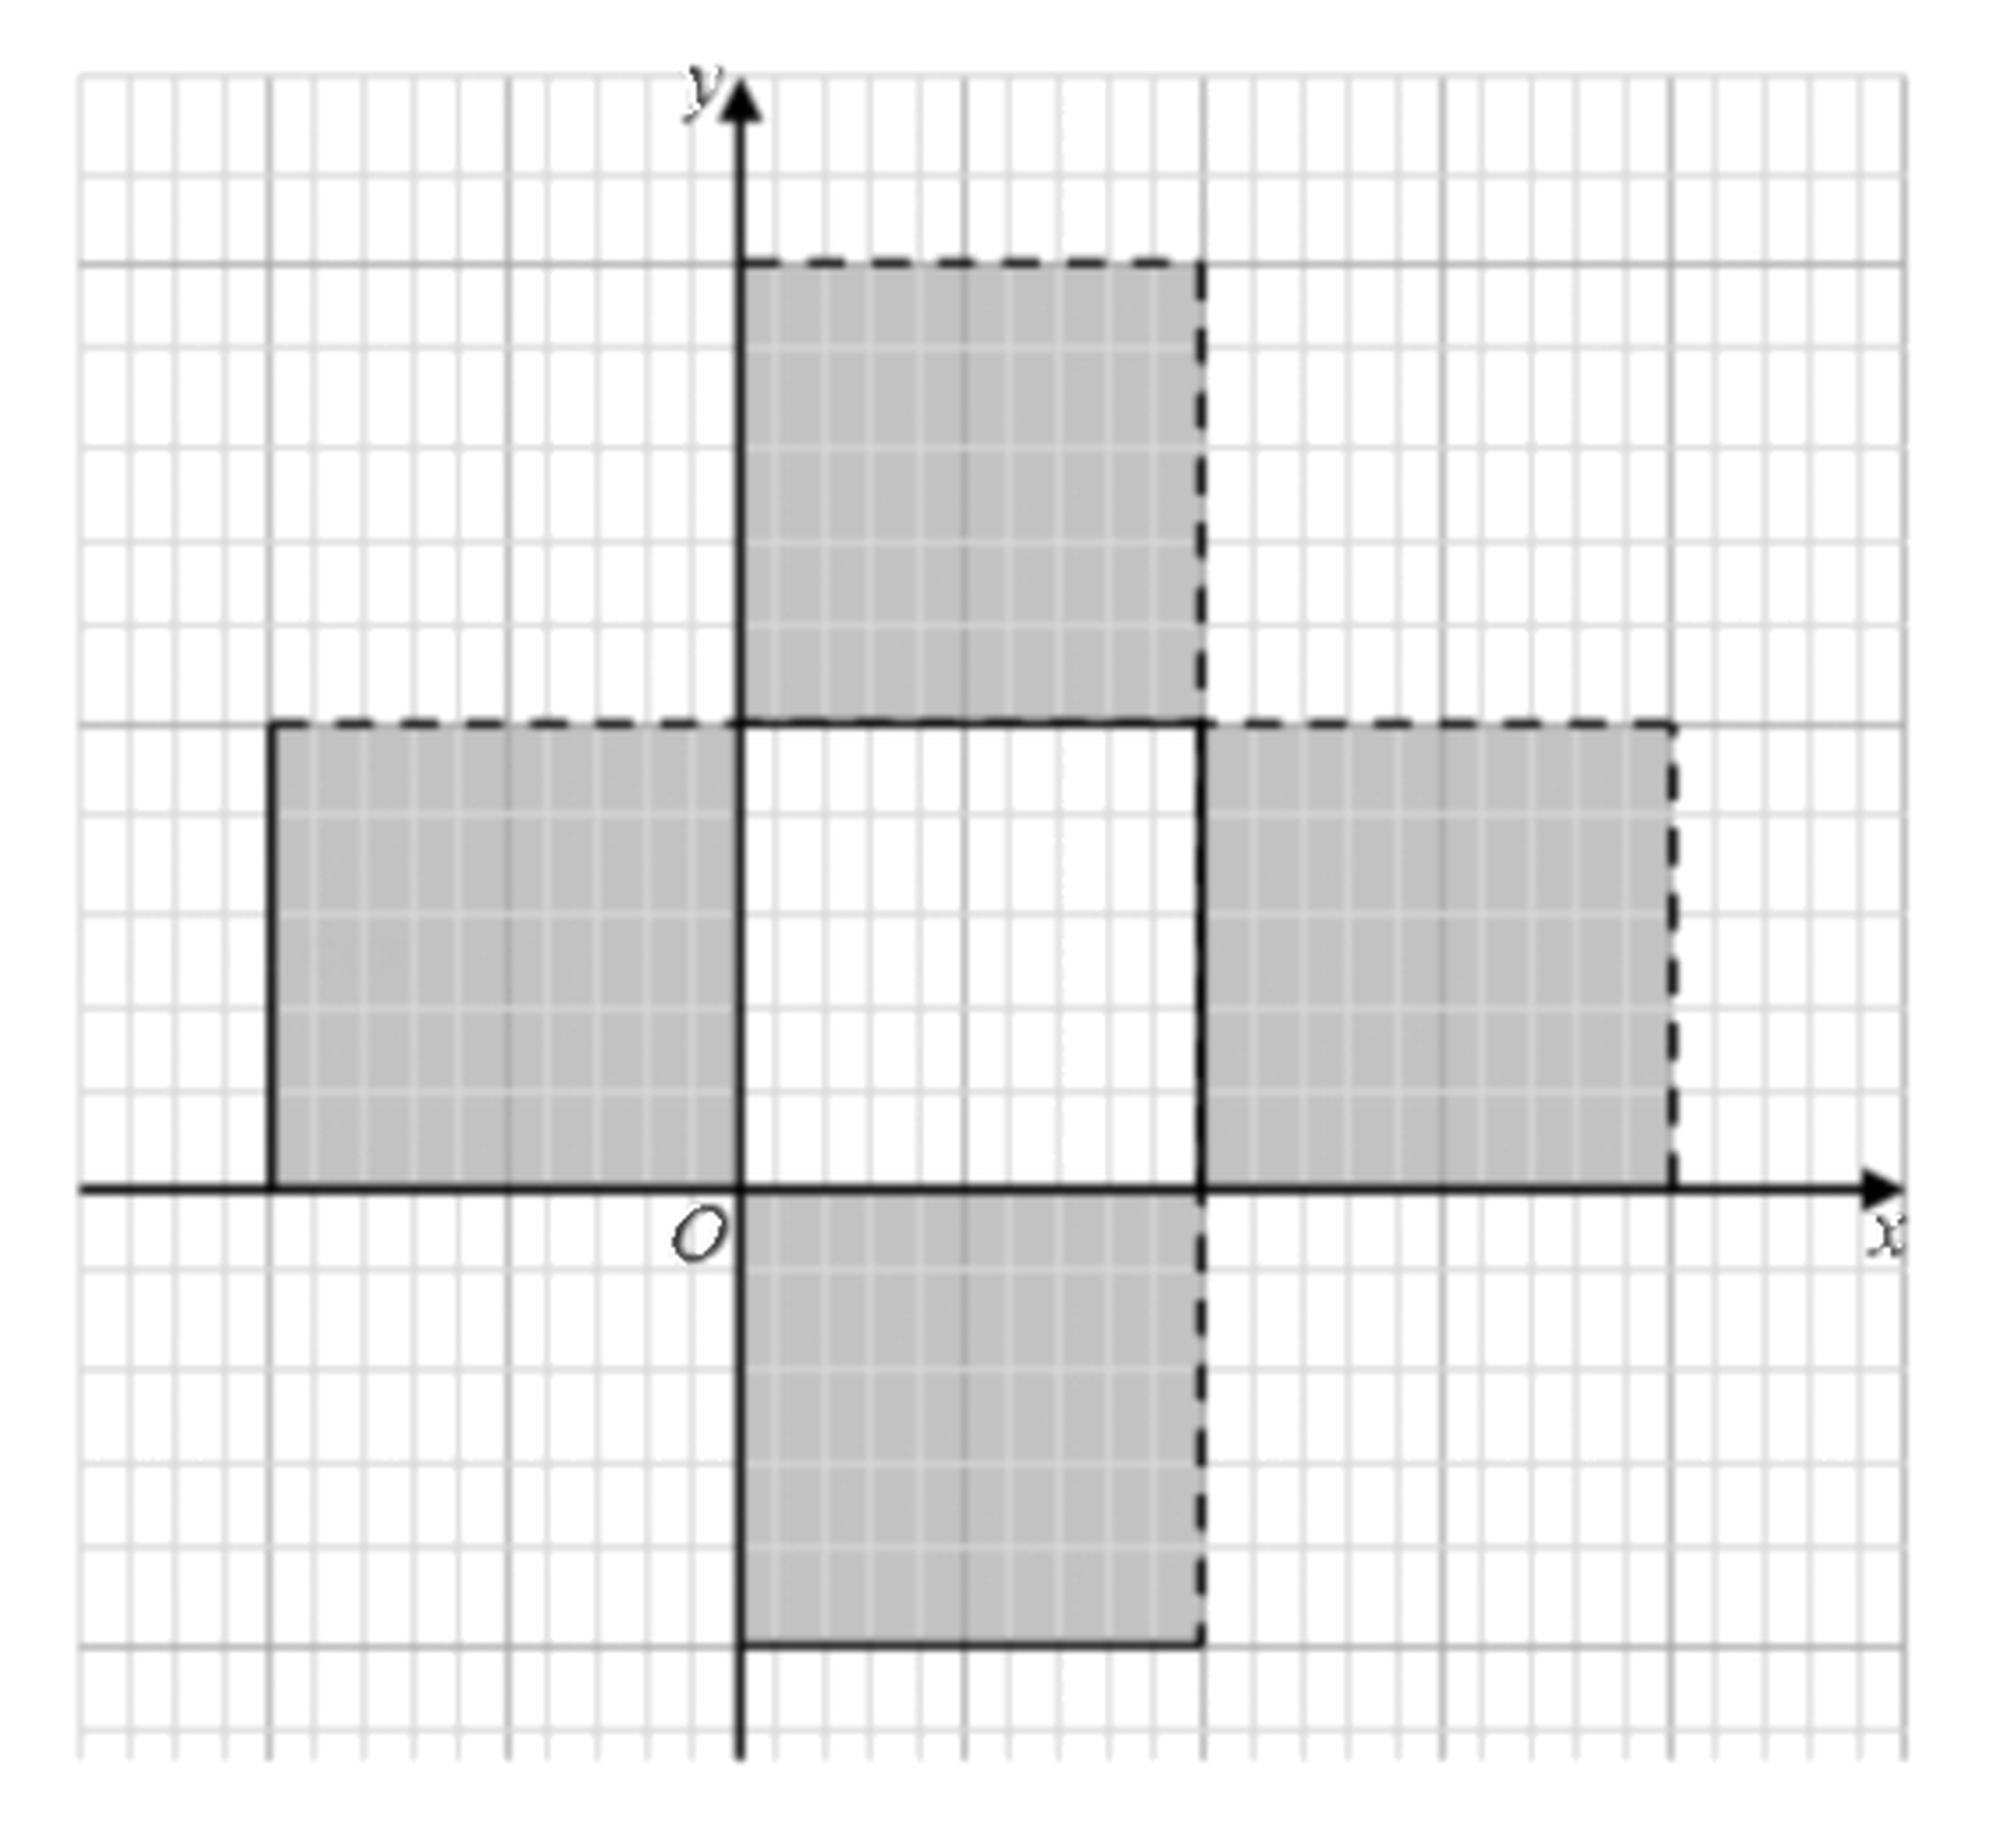
\includegraphics[width=0.34\textwidth]{figures/gao150_q12.png}
\end{center}
\step{总面积为 $1\times4=4$.}
\solend
\fi

\end{enumerate}

\bigsec{二、选择题}

\begin{enumerate}
\setcounter{enumi}{12}

% === Q13 === 答案在解析末句"故选 C"；括号 \mbox{（\quad）} 留空；四选项一行；解析 1 行
\item 设 $x\ne0$，则 $3^{\log_9 x^2}$ 的化简结果是\mbox{（\quad）}

\keepwithprev
A. $x$\qquad B. $\dfrac{1}{x}$\qquad C. $\lvert x\rvert$\qquad D. $\dfrac{1}{\lvert x\rvert}$

\ifanswer
\solbegin
\step{$3^{\log_9 x^2}=3^{\log_3\lvert x\rvert}=\lvert x\rvert$，故选 $C$.}
\solend
\fi

% === Q14 === 题目配图（两函数图像，三版都出）；\needvspace{8cm} 守卫放 \item 之前；"图像"照录；四选项两行两列；解析 2 行，故选 B
\needvspace{8cm}
\item 设 $a>0$ 且 $a\ne1$，$b\in\R$. 若函数 $y=a^{-\lvert x\rvert}$ 与 $y=x^b$ 的大致图像如图所示，则\mbox{（\quad）}

\keepwithprev
A. $0<a<1<b$\qquad\qquad B. $a>1$ 且 $b>1$

C. $0<a<1$ 且 $0<b<1$\qquad\qquad D. $0<b<1<a$

\begin{center}
% 两函数 y=a^{-|x|} 与 y=x^b 大致图像取 04 页右侧，去粉色水印、去色、4× LANCZOS 放大；三版都出
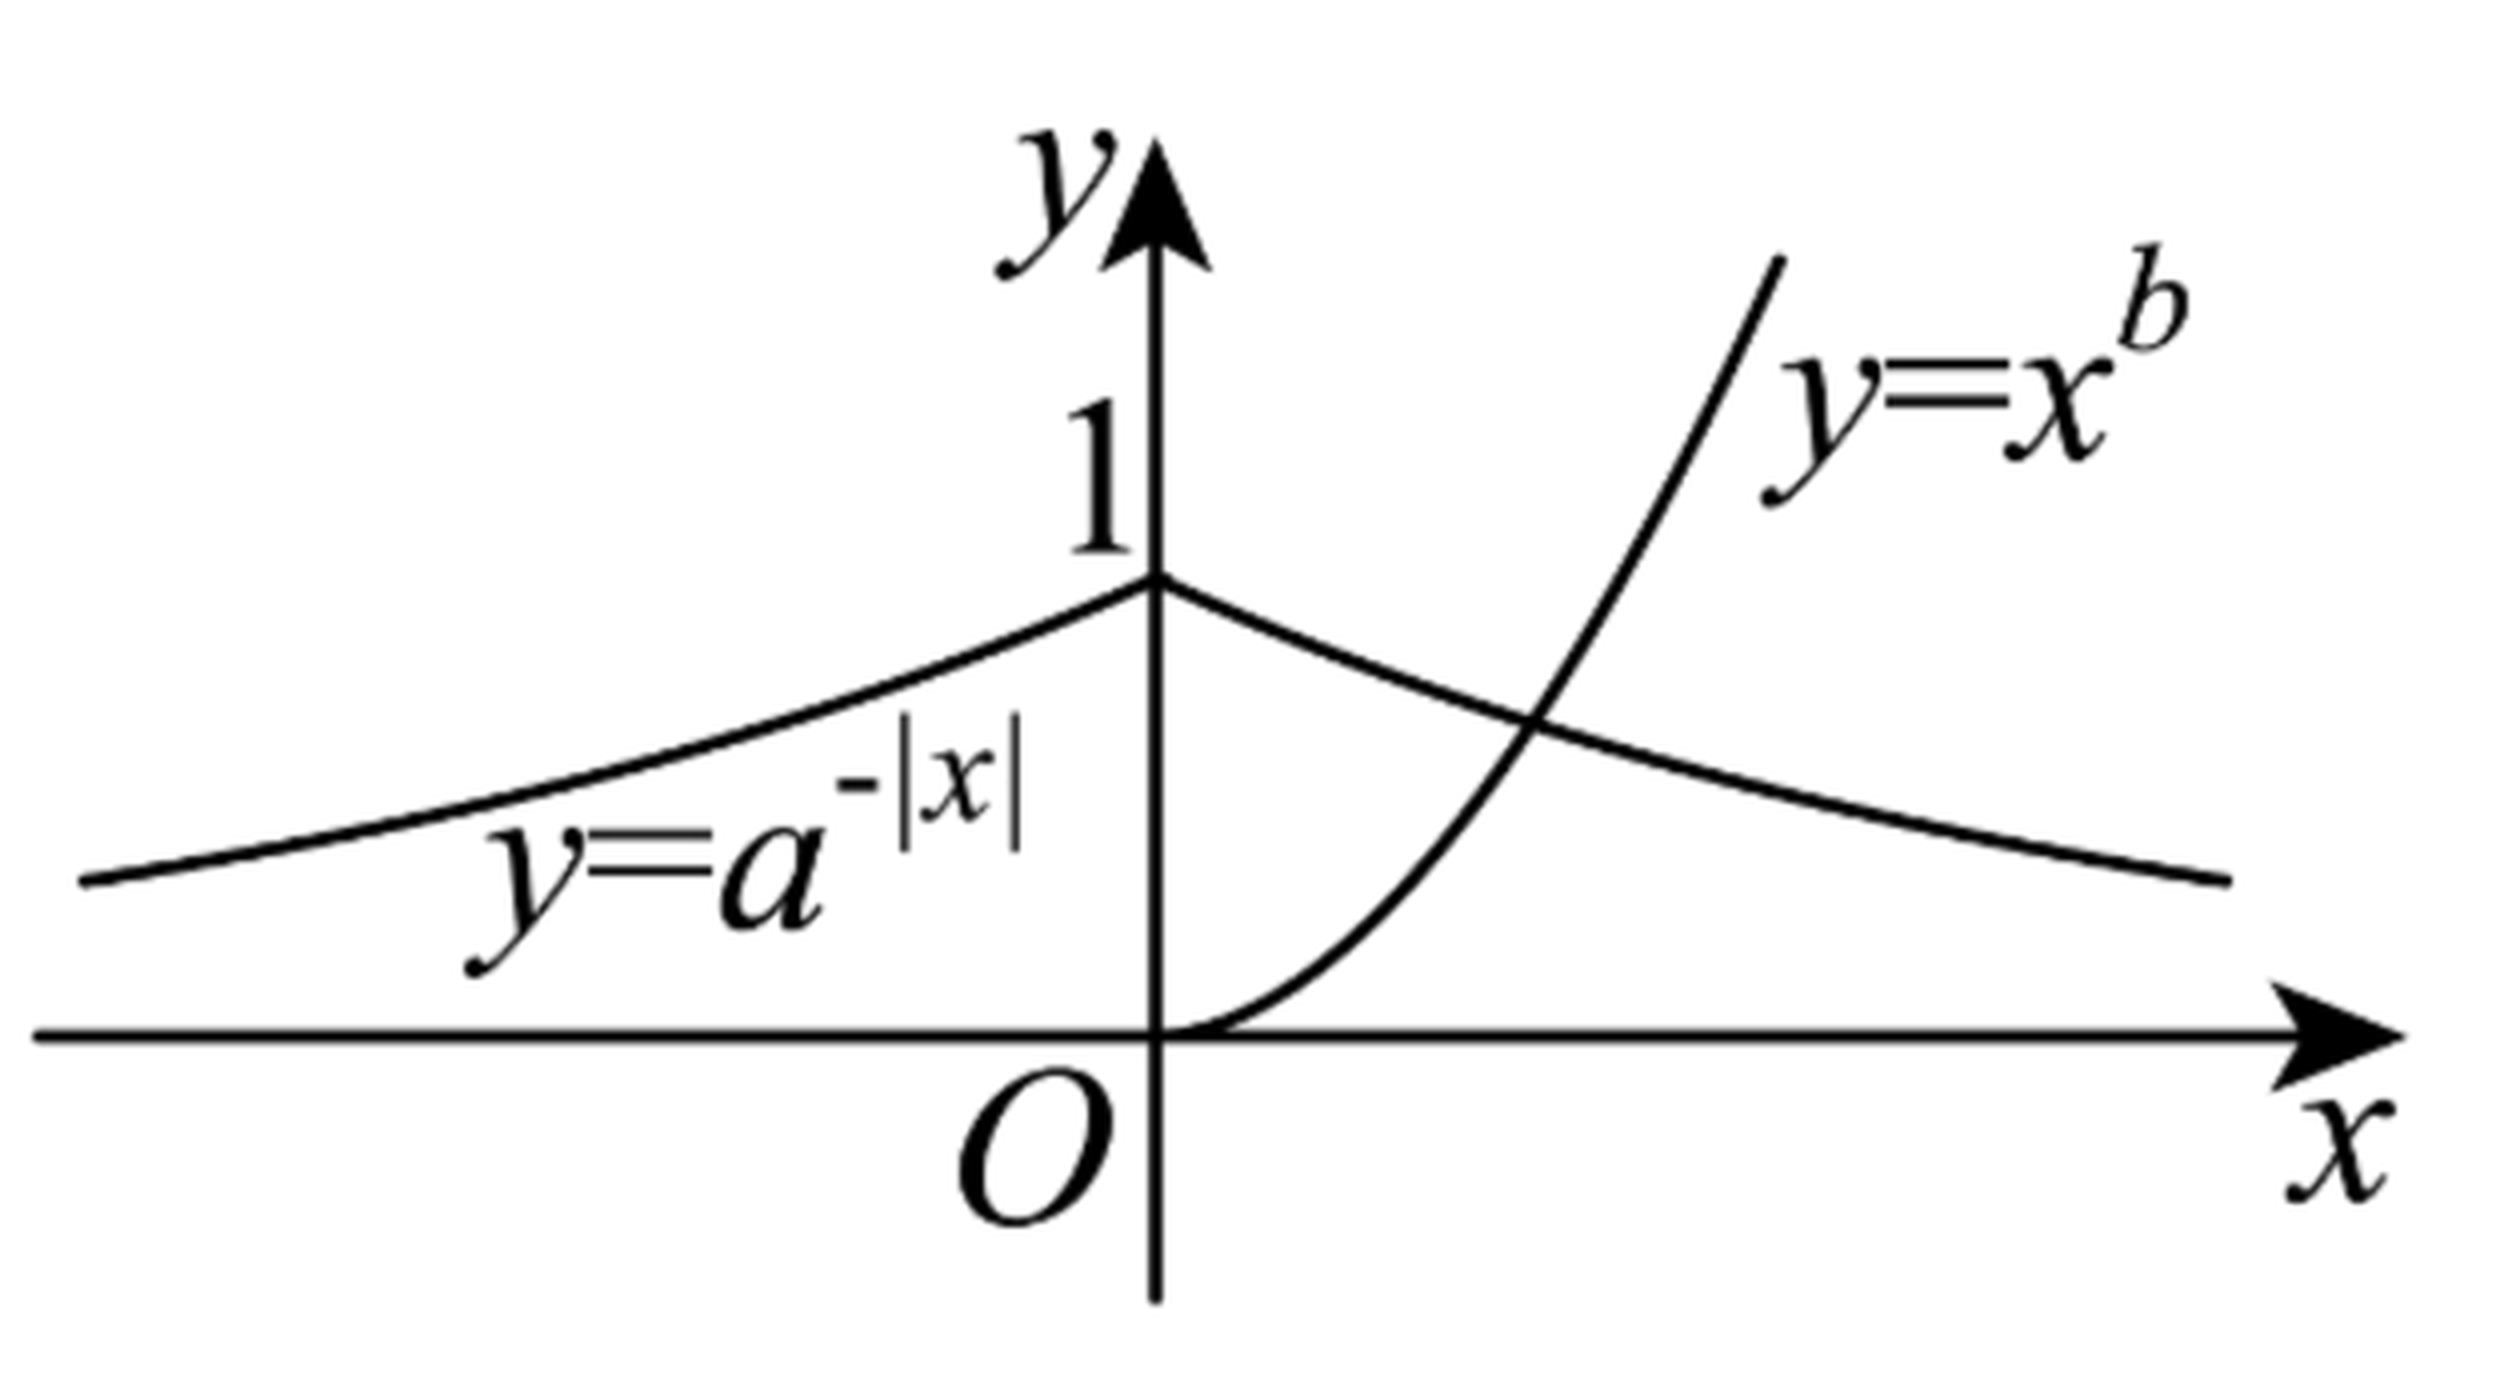
\includegraphics[width=0.40\textwidth]{figures/gao150_q14.png}
\end{center}

\ifanswer
\solbegin
\step{在 $(0,+\infty)$ 上，$y=a^{-x}$ 严格递减，得 $a>1$；}
\step{幂函数 $y=x^b$ 的图像递增且向上弯曲，得 $b>1$；故选 $B$.}
\solend
\fi

% === Q15 === "算术平均值／算术平均数"两处不同照录；四选项两行两列；解析 5 行（续 05 页顶），故选 B
\item 已知两个正数的算术平均值不小于它们的几何平均值，类比有以下结论：三个正数的算术平均数不小于它们的几何平均数，即当 $a,b,c$ 为正实数时，$\dfrac{a+b+c}{3}\geqslant\sqrt[3]{abc}$，当且仅当 $a=b=c$ 时等号成立. 利用上述结论，下列选项中判断正确的是\mbox{（\quad）}

\keepwithprev
A. 若 $x>0$，则 $2x+\dfrac{1}{x^2}\geqslant\dfrac{27}{8}$\qquad\qquad B. 若 $x>0$，则 $x^2+\dfrac{2}{x}\geqslant3$

C. 若 $0<x<1$，则 $x^2(1-x)\geqslant\dfrac{1}{9}$\qquad\qquad D. 若 $0<x<1$，则 $x^2(1-x)\leqslant\dfrac{1}{9}$

\ifanswer
\solbegin
\step{A：取 $x=1$，$2x+\dfrac{1}{x^2}=3<\dfrac{27}{8}$，错误.}
\step{B：$x^2+\dfrac{2}{x}=x^2+\dfrac{1}{x}+\dfrac{1}{x}\geqslant3\sqrt[3]{x^2\cdot\dfrac{1}{x}\cdot\dfrac{1}{x}}=3$，当且仅当 $x=1$ 时取等号，正确.}
\step{C：取 $x=\dfrac{1}{3}$，$x^2(1-x)=\dfrac{2}{27}<\dfrac{1}{9}$，错误.}
\step{D：取 $x=\dfrac{2}{3}$，$x^2(1-x)=\dfrac{4}{27}>\dfrac{1}{9}$，错误.}
\step{故选 $B$.}
\solend
\fi

% === Q16 === "完美集"新定义（弯引号、引号外空格照录）；圈数字①②文本模式；$n\in\N$；四选项两行两列；解析 9 行（6 行 05 页＋3 行 06 页顶），故选 A
\item 已知有限集 $A=\{a_1,a_2,\cdots,a_n\}$（$n\geqslant2$，$n\in\N$）. 若 $A$ 中元素 $a_i$（$i=1,2,\cdots,n$）满足 $a_1+a_2+\cdots+a_n=a_1\cdot a_2\cdots a_n$，就称 $A$ 为 “完美集”. 现有以下两个命题：

①恰有两个元素的 “完美集” 有无穷多个；

②若 $a_i$ 均为正整数，则 “完美集” $A$ 有且只有一个，且 $n=3$.

则\mbox{（\quad）}

\keepwithprev
A. ①和②都是真命题\qquad\qquad B. ①和②都是假命题

C. ①是真命题，②是假命题\qquad\qquad D. ①是假命题，②是真命题

\ifanswer
\solbegin
\step{①由 $a+b=ab\Leftrightarrow(a-1)(b-1)=1$，任取 $a>2$，则 $b=1+\dfrac{1}{a-1}\in(1,2)$，}
\step{得到无穷多个不同的完美集，①真.}
\step{②设 $1\leqslant a_1<a_2<\cdots<a_n$，则 $a_i\geqslant i$.}
\step{若 $n=2$，则 $(a_1-1)(a_2-1)=1$，只能有 $a_1=a_2=2$，与元素互异矛盾.}
\step{若 $n\geqslant4$，则 $a_1a_2\cdots a_n\geqslant a_2a_{n-1}a_n\geqslant2(n-1)a_n>na_n\geqslant a_1+\cdots+a_n$，矛盾.}
\step{当 $n=3$ 时，若 $a_1\geqslant2$，则 $a_1a_2a_3\geqslant6a_3>3a_3\geqslant a_1+a_2+a_3$，矛盾.}
\step{因此 $a_1=1$，$(a_2-1)(a_3-1)=2$，结合 $a_2<a_3$ 得 $a_2=2$，$a_3=3$.}
\step{唯一的完美集为 $\{1,2,3\}$，②真.}
\step{故选 $A$.}
\solend
\fi

\end{enumerate}

\bigsec{三、解答题}

\begin{enumerate}
\setcounter{enumi}{16}

% === Q17 === \varnothing 空集、$B\subseteq A$ 带下划线照录；弯引号内空格照录；解析 7 行
\item 设 $a,b\in\R$. 已知集合 $A=\{x\mid ax^2+3x-a>3\}$，$B=\{x\mid bx=1\}$.

(1) 若 $A=(1,2)$，求 $a$ 的值；

(2) 若 $a=0$，且 “ $x\in A$ ” 是 “ $x\in B$ ” 的必要非充分条件，求 $b$ 的取值范围.

\ifanswer
\solbegin
\step{(1) $A=(1,2)$，则 $a<0$，且 $1,2$ 是方程 $ax^2+3x-a-3=0$ 的两根.}
\step{由 $4a+6-a-3=0$，得 $a=-1$，此时不等式为 $-(x-1)(x-2)>0$，}
\step{解集确为 $(1,2)$.}
\step{(2) $a=0$ 时，$A=(1,+\infty)$，题意等价于 $B\subseteq A$ 且 $B\ne A$.}
\step{当 $b=0$ 时，$B=\varnothing$，符合条件.}
\step{当 $b\ne0$ 时，$B=\left\{\dfrac{1}{b}\right\}$，条件等价于 $\dfrac{1}{b}>1$，解得 $0<b<1$.}
\step{因此 $b$ 的取值范围为 $[0,1)$.}
\solend
\fi

% === Q18 === $p\in\Z$；"图像"（像，有亻）照录；指数 $-2p^2+5p$；解析 8 行（(1) 首行 06 页末＋2 行 07 页顶、(2) 5 行 07 页）
\item 设 $p\in\Z$，已知 $f(x)=x^{-2p^2+5p}$.

(1) 若幂函数 $y=f(x)$ 的图像关于原点成中心对称，且满足 $f(3)<f(4)$，求 $p$ 的值；

(2) 当 $p=-2$ 时，求满足 $f(2x+3)<f(x-4)$ 的 $x$ 的取值范围.

\ifanswer
\solbegin
\step{(1) 图像关于原点成中心对称，得整数 $-2p^2+5p$ 为奇数.}
\step{由 $f(3)<f(4)$，得 $-2p^2+5p>0\Leftrightarrow0<p<\dfrac{5}{2}$，}
\step{结合 $p\in\Z$，得 $p=1$ 或 $p=2$，对应指数分别为 $3$、$2$，所以 $p=1$.}
\step{(2) 当 $p=-2$ 时，$f(x)=\dfrac{1}{x^{18}}$，定义域为 $\{x\in\R\mid x\ne0\}$.}
\step{原不等式要求 $x\ne-\dfrac{3}{2}$ 且 $x\ne4$，}
\step{此时 $\dfrac{1}{(2x+3)^{18}}<\dfrac{1}{(x-4)^{18}}\Leftrightarrow\lvert 2x+3\rvert>\lvert x-4\rvert\Leftrightarrow(2x+3)^2>(x-4)^2$，}
\step{因此 $(x+7)(3x-1)>0\Leftrightarrow x<-7$ 或 $x>\dfrac{1}{3}$，}
\step{排除 $x=4$，得 $x\in(-\infty,-7)\cup\left(\dfrac{1}{3},4\right)\cup(4,+\infty)$.}
\solend
\fi

% === Q19 === $a\in\R$、$g(x)=f(2x+1)+a\cdot f(x)+2$；解析 6 行（(2) 末两行续 08 页顶）
\item 已知 $f(x)=2^x$.

(1) 求方程 $f(2x)-f(x)=6$ 的解；

(2) 设 $a\in\R$，$g(x)=f(2x+1)+a\cdot f(x)+2$，若对于任意 $x\in[-1,1]$，均有 $g(x)\geqslant1$，求 $a$ 的取值范围.

\ifanswer
\solbegin
\step{(1) 令 $t=2^x>0$，则 $t^2-t-6=(t-3)(t+2)=0$，}
\step{由 $t>0$ 得 $t=3$，所以 $x=\log_2 3$.}
\step{(2) 令 $t=2^x$，则 $t\in\left[\dfrac{1}{2},2\right]$，且 $g(x)\geqslant1\Leftrightarrow2t^2+at+1\geqslant0\Leftrightarrow a\geqslant-\left(2t+\dfrac{1}{t}\right)$，}
\step{由基本不等式得 $2t+\dfrac{1}{t}\geqslant2\sqrt{2t\cdot\dfrac{1}{t}}=2\sqrt2$，}
\step{当且仅当 $t=\dfrac{1}{\sqrt2}\in\left[\dfrac{1}{2},2\right]$ 时等号成立，}
\step{因此 $-\left(2t+\dfrac{1}{t}\right)$ 的最大值为 $-2\sqrt2$，所求范围为 $a\in[-2\sqrt2,+\infty)$.}
\solend
\fi

% === Q20 === "极闭集"新定义、3 问，全卷末题；$M\subseteq(0,+\infty)$ 带下划线照录；自定义运算 $x*y$ 星号照录；解析 13 行（9 行 08 页＋4 行 09 页上半）
\item 对于非空实数集 $M\subseteq(0,+\infty)$，若满足以下两个条件：

① $M$ 中至少含有 $2$ 个元素，且 $1\notin M$；

②对于 $M$ 中任意两个不相等的元素 $x$、$y$，定义 $x*y=\dfrac{xy+1}{x+y}$，且 $x*y\in M$.

则称 $M$ 为 “极闭集”.

(1) 分别判断集合 $A=\left\{\dfrac{1}{2},3\right\}$ 与集合 $B=(1,+\infty)$ 是否为 “极闭集” （无需理由）；

(2) 若 $M$ 是 “极闭集”，证明：$M$ 中不可能所有元素都小于 $1$；

(3) 证明：不存在任何有限集是 “极闭集”.

\ifanswer
\solbegin
\step{(1) $A$ 不是 “极闭集”，$B$ 是 “极闭集”.}
\step{(2) 假设 $M$ 中所有元素都小于 $1$，取其中两个不相等的元素 $x$、$y$，}
\step{则 $x*y-1=\dfrac{(1-x)(1-y)}{x+y}>0$，}
\step{这与 $x*y\in M$ 且 $M$ 中所有元素都小于 $1$ 矛盾.}
\step{(3) 假设有限集 $M$ 是 “极闭集”，}
\step{由 (2) 及 $1\notin M$，得 $M$ 中存在大于 $1$ 的元素.}
\step{若 $M$ 中有小于 $1$ 的元素，取其中最大的一个为 $a$，另取 $b\in M$ 且 $b>1$，}
\step{则 $a*b-a=\dfrac{1-a^2}{a+b}>0, a*b-1=\dfrac{(a-1)(b-1)}{a+b}<0$，}% 半角逗号在两个数学式组之间，全稿惯例、非笔误，照录
\step{于是 $a<a*b<1$ 且 $a*b\in M$，与 $a$ 的最大性矛盾.}
\step{若 $M$ 中没有小于 $1$ 的元素，则 $M\subseteq(1,+\infty)$.}
\step{取 $a=\min M$，另取 $b\in M$ 且 $b\ne a$，则 $a*b-a=\dfrac{1-a^2}{a+b}<0$，}
\step{于是 $a*b<a$ 且 $a*b\in M$，与 $a$ 的最小性矛盾.}
\step{因此不存在任何有限集是 “极闭集”.}
\solend
\fi

\end{enumerate}

\end{document}
"
% 紧凑版：xelatex "\def\iscompact{1}% 高一150_曹杨二中_期中.tex
%   —— 高一上数学"2026-2027 年曹杨二中高一上期中"（试卷版/答案版/紧凑版）
% 试卷版：xelatex 高一150_曹杨二中_期中.tex
% 答案版：xelatex "\def\isanswer{1}% 高一150_曹杨二中_期中.tex
%   —— 高一上数学"2026-2027 年曹杨二中高一上期中"（试卷版/答案版/紧凑版）
% 试卷版：xelatex 高一150_曹杨二中_期中.tex
% 答案版：xelatex "\def\isanswer{1}\input{高一150_曹杨二中_期中.tex}"
% 紧凑版：xelatex "\def\iscompact{1}\input{高一150_曹杨二中_期中.tex}"
%
% ① 原始材料：微信公众号"魔都数学加油站"文章，连载"27学年高一150"，原文标题
% "27学年高一150——2026-2027年上海市曹杨二中高一上期中"；
% 原文链接：https://mp.weixin.qq.com/s/xlQxmik8TZXR87RC6MnCrw 。
% 正文为 9 张 PNG 页（01/02/04/06/07/09 为 2560×3620，03/05/08 为 4762×6735，
% 同一篇各页分辨率混排，逐页按各自分辨率裁图核对，别按预览比例换算裁框）。
% 体例：讲评版——全 18 题均印【解析】（逐题核实，见 ② ②）。
% 题目、答案、解析均据原图转录；卷面粉红色/红色水印"魔都数学加油站"及公众号页脚未录入。
% 全卷插图清单（逐页通读 9 页确认）：3 幅——
%   · Q11 题目配图（指数函数曲线图，02 页右侧：x/y 轴、O、y=2^x 与 y=2^{x+1}
%     两曲线、A/B/C 三点、刻度 1/2、等边三角形 ABC），三版都出，裁 figures/gao150_q11.png；
%   · Q12 解析配图（高斯函数取整 [x]^2+[y]^2=1 方格阴影区域图，04 页顶部：4 个边长 1
%     的正方形组成的十字形阴影），解析"作出平面区域如图所示"处，仅答案版出，
%     放 \ifanswer 内 \step 之间，裁 figures/gao150_q12.png；
%   · Q14 题目配图（两函数 y=a^{-|x|} 与 y=x^b 大致图像，04 页右侧：x/y 轴、O、
%     y 轴刻度 1、一递减曲线一递增上翘曲线），三版都出，裁 figures/gao150_q14.png；
%   其余各页逐页确认无其它题目配图、无表格；Q11/Q12 解析"如图所示"对应的就是上列
%   已裁的图，不重复裁；09 页上半为 Q20(3) 解析续尾、下半仅水印、无正文。
%   3 图均取自原卷截图，去粉色水印、去色、4× LANCZOS 放大。
%
% 卷首标题：原卷印作"2026-2027 年曹杨二中高一上期中"，年份区间按全稿惯例排 en dash；
% 原卷卷面未印副标题，本稿按同期中卷知识模块口径补出"集合与常用逻辑用语、不等式、函数"。
%
% 题号体例（逐页核实定稿）：本卷共 18 题——一、填空题 3—12（10 题）、
% 二、选择题 13—16（4 题）、三、解答题 17—20（4 题）。
% 三节分别 \setcounter{enumi}{2}／{12}／{16}。原卷从第 3 题起、无第 1、2 题，
% 本稿保留原题号；全卷末题为第 20 题（"极闭集"新定义、3 问），无 Q21、无附加题节。
%
% ② 与原卷的排版差异：
%   ① 原文从第 3 题起，本稿保留原题号；共 18 题三节，解答题只有 4 题到 20；
%   ② 全 18 题均印【解析】，用 \solbegin…\solend；逐题核实无只印【答案】或
%      答案印题干括号内的题；四道选择题答案在解析末句"故选 X"（Q13 选 C、
%      Q14 选 B、Q15 选 B、Q16 选 A，逐个放大复核）、括号 \mbox{（\quad）} 留空、
%      不另提 \ans{}；答案版【答案】/【解析】标记数 = 18 = 全卷题数；
%   ③ 原卷卷面未印副标题，本稿按知识模块口径补出；
%   ④ 原卷填空横线按全稿惯例排 \blankline[4.4em]；选择题括号排 \mbox{（\quad）}、
%      选项段前按惯例加 \keepwithprev；解答题不留作答区、不加 \anspace（原卷为讲评版）；
%   ⑤ 数集黑板粗体：Q4"m\in R"、Q5"a,b\in R"、Q6"a,b,c\in R"、Q7"a\in R"、
%      Q10"a\in R"、Q14"b\in R"、Q17"a,b\in R"、Q18"p\in Z"／定义域"x\in R"、
%      Q19"a\in R"、Q16"n\in N" 原卷印斜体 R/Z/N，按全稿惯例归一 \R／\Z／\N；
%      绝对值排 \lvert…\rvert（Q7 |x+4|+|x-3|、Q11 |AB|／|CD|、Q13 |x|、
%      Q18 |2x+3|／|x-4|），集合描述竖线排 \mid（Q3、Q12、Q17、Q18、Q20），
%      不等号按全稿惯例排 \leqslant／\geqslant；补集照原卷上划线排 \overline{A}
%      （Q3 题干＋解析共 2 处）；空集符号 \varnothing（Q17 解析(2)）；
%      子集 \subset（单线⊂）／\subseteq（带下划线⊆）逐处照录，本卷 3 处子集
%      符号均印带下划线 ⊆、照录 \subseteq（Q20 题干、Q20 解析(3)、Q17 解析(2)，
%      见 ④），无 \subset 用例；
%   ⑥ 判别式 Δ/△：逐页通读 9 页，本卷无一元二次判别式算式，故无 Δ/△ 混用可照录
%      （"高 \Delta／扁 \triangle"口径备查，参照 高一142／144／145／146／148／149
%      头注④）；本卷仅 Q11 题干与解析共 2 处几何三角形符号 △ABC，逐处放大并排
%      确认两处同形、印近等边粗线三角（非判别式），照录 \triangle（见 ④）；
%   ⑦ 中文弯引号照录：Q12"数学王子"、Q16"完美集"（题干＋①②两命题，引号外
%      留空格）、Q17" x∈A "" x∈B "（引号内空格）、Q20"极闭集"（题干条件、
%      三问与解析，引号外留空格）；注释里一律 ASCII 引号；数学式内 CJK 用 \text{}
%      （Q3 集合描述"且"用 \text{ 且 }）；
%   ⑧ 半角逗号在数学组之间是全稿惯例、非笔误，逐处照录（Q17 解析"1,2 是方程…
%      两根"、Q20 解析(3)">0, a*b-1=…<0" 两式之间等）；行末西文句点 ASCII `.`；
%      行中全角逗号／顿号照录（Q12"之一、享有"、Q18 解析"3、2"、Q20"x、y"）；
%   ⑨ "图像／图象"逐处放大核：全卷 9 处均印"图像"（像，有亻）、未见"图象"——
%      Q4 题干 1、Q11 题干 2＋解析 1、Q14 题干 1＋解析 1、Q18 题干 1＋解析 1；
%      同卷"第二象限""象限"用"象"（无亻）。逐处照录未统一改动（放大 01/02/04/06
%      页 /tmp/gao150/z/p01_q4_tuxiang2.png、p04_q14_tuxiang2.png、
%      p02_q11_lines.png 确认）；子题标号 (1)(2)(3) 半角括号照录；圈数字①②
%      在文本模式（Q16 两命题与解析、Q20 两条件与三问及解析）按 common.sty
%      划入 CJK 字符类渲染，进数学式用 \text{①}；
%   ⑩ Q20 新定义 x*y=\dfrac{xy+1}{x+y} 的 * 是自定义运算（星号），照录；
%      \left…\right 不得拆到不同 $…$ 组（Q19"\left(2t+\frac1t\right)"、
%      Q20 题干"A=\left\{\frac12,3\right\}"等）；Q8 嵌套根号
%      \sqrt{\frac2x+\frac{16}{1-2x}}、Q9 对数连加 \log_2 A 等复杂式照录别简化；
%   ⑪ 一条 \step = 原卷解析的一个印刷行，cases 块整体算一个印刷行；别并折行、
%      别拆行。Q4 三行、Q8 五行、Q11 九行、Q12 四行（两行各含四个 cases 块）、
%      Q15 五行、Q16 九行、Q18 八行、Q20 十三行均按印刷行逐条断，不丢行；
%   ⑫ 配图：Q11／Q14 题目配图（三版都出）放 \item 内题干之后 \begin{center}，
%      大图块加 \needvspace{8cm} 守卫把整块推走（守卫放 \item 之前，见
%      高一145 Q14/Q20 成例与切页审计 B 类坑）；Q12 解析配图（仅答案版出）
%      放 \ifanswer 内 \solbegin…\solend 的 \step 之间（高一73 第16题成例）；
%   ⑬ 跨页续印按题合并：见 ⑥；
%   ⑭ 原卷解析内无红色"法一／法二"之类小标题，故本卷无 \stepm；红色水印
%      "魔都数学加油站"不录入；Q12 解析"作出平面区域如图所示"对应的图即
%      ① 所列 gao150_q12.png（04 页顶部），不重复裁；Q11 解析"如图所示"对应
%      题目配图 gao150_q11.png，不另裁。
%
% ③ 行数复核：一条 \step／\stepm = 原卷解析的一个印刷行，cases 块作一个印刷行计。
%   逐题数（主会话逐页核对定稿）：Q3：1；Q4：3；Q5：2；Q6：1；Q7：2；Q8：5；
%   Q9：1；Q10：3；Q11：9；Q12：4；Q13：1；Q14：2；Q15：5；Q16：9；
%   Q17：7；Q18：8；Q19：6；Q20：13。
%   合计 82 条 \step（本卷无 \stepm：解析内无红色"法一／法二"类小标题），
%   与原卷逐题印刷行相等。全卷 18 题均设 \solbegin…\solend，答案版
%   【答案】/【解析】标记数 = 18 = 全卷题数。
%
% ④ 判别式／三角形／子集符号结论（逐处放大原图照录、不得统一，主会话像素级复核）：
%   判别式：逐页通读 9 页，本卷无一元二次判别式 Δ/△ 算式（Q18 讨论幂函数指数
%     奇偶、不用判别式；Q9／Q19／Q20 亦无），头注 ② ⑥ 的"高 \Delta／扁 \triangle"
%     口径在本卷无对应处（参照 高一142／144／145／146／148／149 头注④，仅备查）。
%   几何三角形符号：Q11 题干"使得 △ABC 为等边三角形"（02 页末）与解析
%     "因为 △ABC 为等边三角形，则 CD⊥AB"（03 页）共 2 处，放大 02/03 页
%     /tmp/gao150/z/q11_tri_montage2.png 并排确认两处同形、印近等边粗线三角
%     （h/w≈0.98、非"高>宽"的判别式 \Delta），照录 \triangle（与 高一105
%     "使得 \triangle ABC 为等边三角形" 同短语成例、高一149 几何三角形照录
%     \triangle 口径一致），不引入 \Delta。
%   子集／补集：Q20 题干"$M\subseteq(0,+\infty)$"（08 页）、Q20 解析(3)
%     "则 $M\subseteq(1,+\infty)$"（09 页）、Q17 解析(2)"题意等价于 $B\subseteq A$
%     且 $B\ne A$"（06 页）共 3 处子集符号，逐处放大（/tmp/gao150/z/p08_q20_stem.png、
%     p09_q20_sub.png、p06_q17_sub.png）确认均印带下划线 ⊆，照录 \subseteq；
%     本卷未见单线 ⊂（\subset）之对应处。Q3 题干与解析共 2 处补集照原卷上划线
%     排 \overline{A}；Q17 解析(2) 空集印 ∅、照录 \varnothing（Q7"解集为空集"
%     为中文词、非符号，照录文字）；集合描述竖线 \mid；数集 \R／\Z／\N 归一见 ② ⑤。
%
% ⑤ 存疑照录（放大原图确认，照录未改、正文对应处另有 % 注）：
%   1. Q8 解析第 4 行"所以 $y=\frac1x+\frac{8}{1-2x}$ 的最小值为 18" —— 上文
%      并未定义 $y$，且题面求的是 $\sqrt{\frac2x+\frac{16}{1-2x}}$ 的最小值；
%      按上下文该行应为 $\frac1x+\frac{8}{1-2x}$ 的最小值为 18（$y$ 疑为原卷
%      衍字／笔误），放大 02 页 /tmp/gao150/z/p02_q8_y.png 确认，照录未改。
%   2. Q20 解析(3)"$a*b-a=\frac{1-a^2}{a+b}>0, a*b-1=\frac{(a-1)(b-1)}{a+b}<0$"
%      两式之间的逗号原卷印半角 ,（非全角），按全稿惯例"半角逗号在数学组之间"
%      照录未改（放大 08 页 /tmp/gao150/z/p08_q20_sol8.png 确认）。
%   3. Q15 题干"两个正数的算术平均值…几何平均值"与"三个正数的算术平均数…
%      几何平均数"两处"值／数"用字不同，逐处照录未统一（放大 04 页确认）。
%   4. "图像／图象"全卷 9 处均印"图像"（像，有亻）、未见"图象"，逐处放大核实
%      照录、未统一改动（见 ② ⑨）；本卷判别式 Δ/△ 无用例、几何三角形 2 处
%      照录 \triangle（见 ④）。
%   全卷除此 4 类外未发现其它笔误／自相矛盾处；18 题均印【解析】、无只印【答案】
%   或答案印题干括号内的题（见 ② ②）。
%
% ⑥ 跨页续印按题合并说明（逐页核实定稿）：Q3/4/5/6/7 题干＋解析在 01 页；
%   Q8 题干＋解析 5 行、Q9 题干＋解析 1 行在 02 页上半；Q10 题干＋解析 3 行
%   在 02 页下半；Q11 题干（前两行）＋配图在 02 页下半、题干续"三角形，则点 C
%   的纵坐标为___"与解析 9 行全在 03 页上半（解析"如图所示"对应题目配图）；
%   Q12 题干＋解析 4 行在 03 页下半，解析配图（方格阴影）续印在 04 页顶部；
%   "二、选择题"标题在 04 页中部；Q13 题干＋选项＋解析、Q14 题干＋选项＋
%   配图＋解析在 04 页；Q15 题干＋四选项在 04 页末、解析 5 行续 05 页上半；
%   Q16 题干＋①②两命题＋"则(  )"＋四选项＋解析前 6 行在 05 页、解析末 3 行
%   （"因此 a_1=1…②真""故选 A"）续 06 页顶部；"三、解答题"标题在 06 页；
%   Q17 题干(1)(2)＋解析(1) 3 行＋解析(2) 首行在 06 页、解析(2) 续 3 行
%   在 06 页下半；Q18 题干(1)(2)＋解析(1) 首行在 06 页末、解析(1) 续 2 行＋
%   解析(2) 5 行在 07 页上半；Q19 题干(1)(2)＋解析(1) 2 行＋解析(2) 前 2 行
%   在 07 页下半、解析(2) 末 2 行续 08 页顶部；Q20 题干（新定义＋①②两条件）
%   ＋三问＋解析(1)(2)(3) 前 9 行在 08 页、解析(3) 末 4 行续 09 页上半，
%   末行"因此不存在任何有限集是极闭集"为全卷收尾（09 页下半仅水印、无正文）。
%   本稿按题连排，不丢行、不并折行；全卷末题为第 20 题，无 Q21、无附加题节。
%
\documentclass[a4paper,11pt]{article}
\usepackage{common}

\begin{document}

\examtitlest[3]{2026--2027 年曹杨二中高一上期中}{集合与常用逻辑用语、不等式、函数}

\bigsec{一、填空题}

\begin{enumerate}
\setcounter{enumi}{2}

% === Q3 === 补集上划线 \overline{A}（题干＋解析各 1 处）；集合描述竖线 \mid、数学式内"且"用 \text{}；解析 1 行
\item 设全集 $U=\{1,2,3,4,5\}$，集合 $A=\{x\mid x^2-3x\leqslant0\text{ 且 }x\in U\}$，则 $\overline{A}=$\blankline[4.4em].

\ifanswer
\solbegin
\step{$x^2-3x\leqslant0\Leftrightarrow0\leqslant x\leqslant3$，所以 $A=\{1,2,3\}$，$\overline{A}=\{4,5\}$.}
\solend
\fi

% === Q4 === "图像"（像，有亻）逐处照录、同句"第二象限"用"象"（无亻）；解析 3 行
\item 设 $m\in\R$. 若幂函数 $y=(m^2-5m+1)x^{m+1}$ 的图像经过第二象限，则 $m=$\blankline[4.4em].

\ifanswer
\solbegin
\step{幂函数的系数为 1，故 $m^2-5m+1=1\Rightarrow m=0$ 或 $m=5$.}
\step{$m=0$ 时，$y=x$ 不经过第二象限；}
\step{$m=5$ 时，$y=x^6$ 经过第二象限，因此 $m=5$.}
\solend
\fi

% === Q5 === 解析 2 行
\item 设 $a,b\in\R$. 若 $a^2+\dfrac{b^2}{4}=1$，则 $ab$ 的最大值为\blankline[4.4em].

\ifanswer
\solbegin
\step{$1-ab=\left(a-\dfrac{b}{2}\right)^2\geqslant0$，即 $ab\leqslant1$；}
\step{当 $a=\dfrac{\sqrt2}{2}$，$b=\sqrt2$ 时取等号，最大值为 1.}
\solend
\fi

% === Q6 === 解析 1 行
\item 设 $a,b,c\in\R$. 若等式 $2x^2-3x-2=a(x-1)^2+b(x-1)+c$ 恒成立，则 $a-b+c=$\blankline[4.4em].

\ifanswer
\solbegin
\step{令 $x=0$，得 $a-b+c=-2$.}
\solend
\fi

% === Q7 === 绝对值 \lvert…\rvert；解析 2 行
\item 设 $a\in\R$. 若关于 $x$ 的不等式 $\lvert x+4\rvert+\lvert x-3\rvert<a$ 的解集为空集，则 $a$ 的取值范围是\blankline[4.4em].

\ifanswer
\solbegin
\step{$\lvert x+4\rvert+\lvert x-3\rvert\geqslant\lvert(x+4)-(x-3)\rvert=7$，当 $-4\leqslant x\leqslant3$ 时取等号.}
\step{原不等式的解集为空集当且仅当 $a\leqslant7$，即 $a\in(-\infty,7]$.}
\solend
\fi

% === Q8 === 嵌套根号 \sqrt{\frac{2}{x}+\frac{16}{1-2x}} 照录别简化；解析 5 行
\item 设 $x\in\left(0,\dfrac{1}{2}\right)$，则 $\sqrt{\dfrac{2}{x}+\dfrac{16}{1-2x}}$ 的最小值为\blankline[4.4em].

\ifanswer
\solbegin
\step{因为 $x\in\left(0,\dfrac{1}{2}\right)$，所以 $1-2x>0$，又 $2x+1-2x=1$，}
\step{所以 $\left(\dfrac{1}{x}+\dfrac{8}{1-2x}\right)(2x+1-2x)=10+\dfrac{1-2x}{x}+\dfrac{16x}{1-2x}$}
\step{$\geqslant10+2\sqrt{\dfrac{1-2x}{x}\cdot\dfrac{16x}{1-2x}}=18$，}
\step{当且仅当 $\dfrac{1-2x}{x}=\dfrac{16x}{1-2x}$ 即 $x=\dfrac{1}{6}$ 时取等号，所以 $y=\dfrac{1}{x}+\dfrac{8}{1-2x}$ 的最小值为 18，}% 原卷此处径写 $y=\frac1x+\frac{8}{1-2x}$（上文未定义 $y$、且与题面根式不符），疑笔误，放大 02 页确认，照录未改（见 ⑤）
\step{所以 $\sqrt{\dfrac{2}{x}+\dfrac{16}{1-2x}}$ 的最小值为 6.}
\solend
\fi

% === Q9 === 对数连加 \log_2 A 等复杂式照录别简化；解析 1 行
\item 记 $A=1\times2\times3\times\cdots\times2026$，则 $\dfrac{1}{\log_2 A}+\dfrac{1}{\log_3 A}+\dfrac{1}{\log_4 A}+\cdots+\dfrac{1}{\log_{2026}A}=$\blankline[4.4em].

\ifanswer
\solbegin
\step{原式 $=\log_A 2+\cdots+\log_A 2026=\log_A(2\times3\times\cdots\times2026)=\log_A A=1$.}
\solend
\fi

% === Q10 === "严格减函数／不恒为负／⇔"照录；解析 3 行
\item 设 $a\in\R$，$f(x)=\dfrac{ax+1}{x+2}$. 若函数 $y=f(x)$ 在 $[1,+\infty)$ 上是严格减函数，且在 $[1,+\infty)$ 上的函数值不恒为负，则 $a$ 的取值范围是\blankline[4.4em].

\ifanswer
\solbegin
\step{当 $1\leqslant x_1<x_2$ 时，$f(x_2)-f(x_1)=\dfrac{(2a-1)(x_2-x_1)}{(x_1+2)(x_2+2)}$，故严格递减 $\Leftrightarrow a<\dfrac{1}{2}$.}
\step{此时最大函数值为 $f(1)$，函数值不恒为负 $\Leftrightarrow f(1)=\dfrac{a+1}{3}\geqslant0\Leftrightarrow a\geqslant-1$，}
\step{得 $a\in\left[-1,\dfrac{1}{2}\right)$.}
\solend
\fi

% === Q11 === 题目配图（指数函数曲线，三版都出）；\needvspace{8cm} 守卫放 \item 之前；"图像"照录、几何三角形 \triangle；解析 9 行（全在 03 页）
\needvspace{8cm}
\item 如图，点 $C$ 是函数 $y=2^x$ 的图像上的一点，若存在平行于 $x$ 轴的直线 $l$ 分别与函数 $y=2^x$ 和 $y=2^{x+1}$ 的图像相交于点 $A$、$B$，使得 $\triangle ABC$ 为等边三角形，则点 $C$ 的纵坐标为\blankline[4.4em].

\begin{center}
% 指数函数曲线图取 02 页右侧，去粉色水印、去色、4× LANCZOS 放大；三版都出
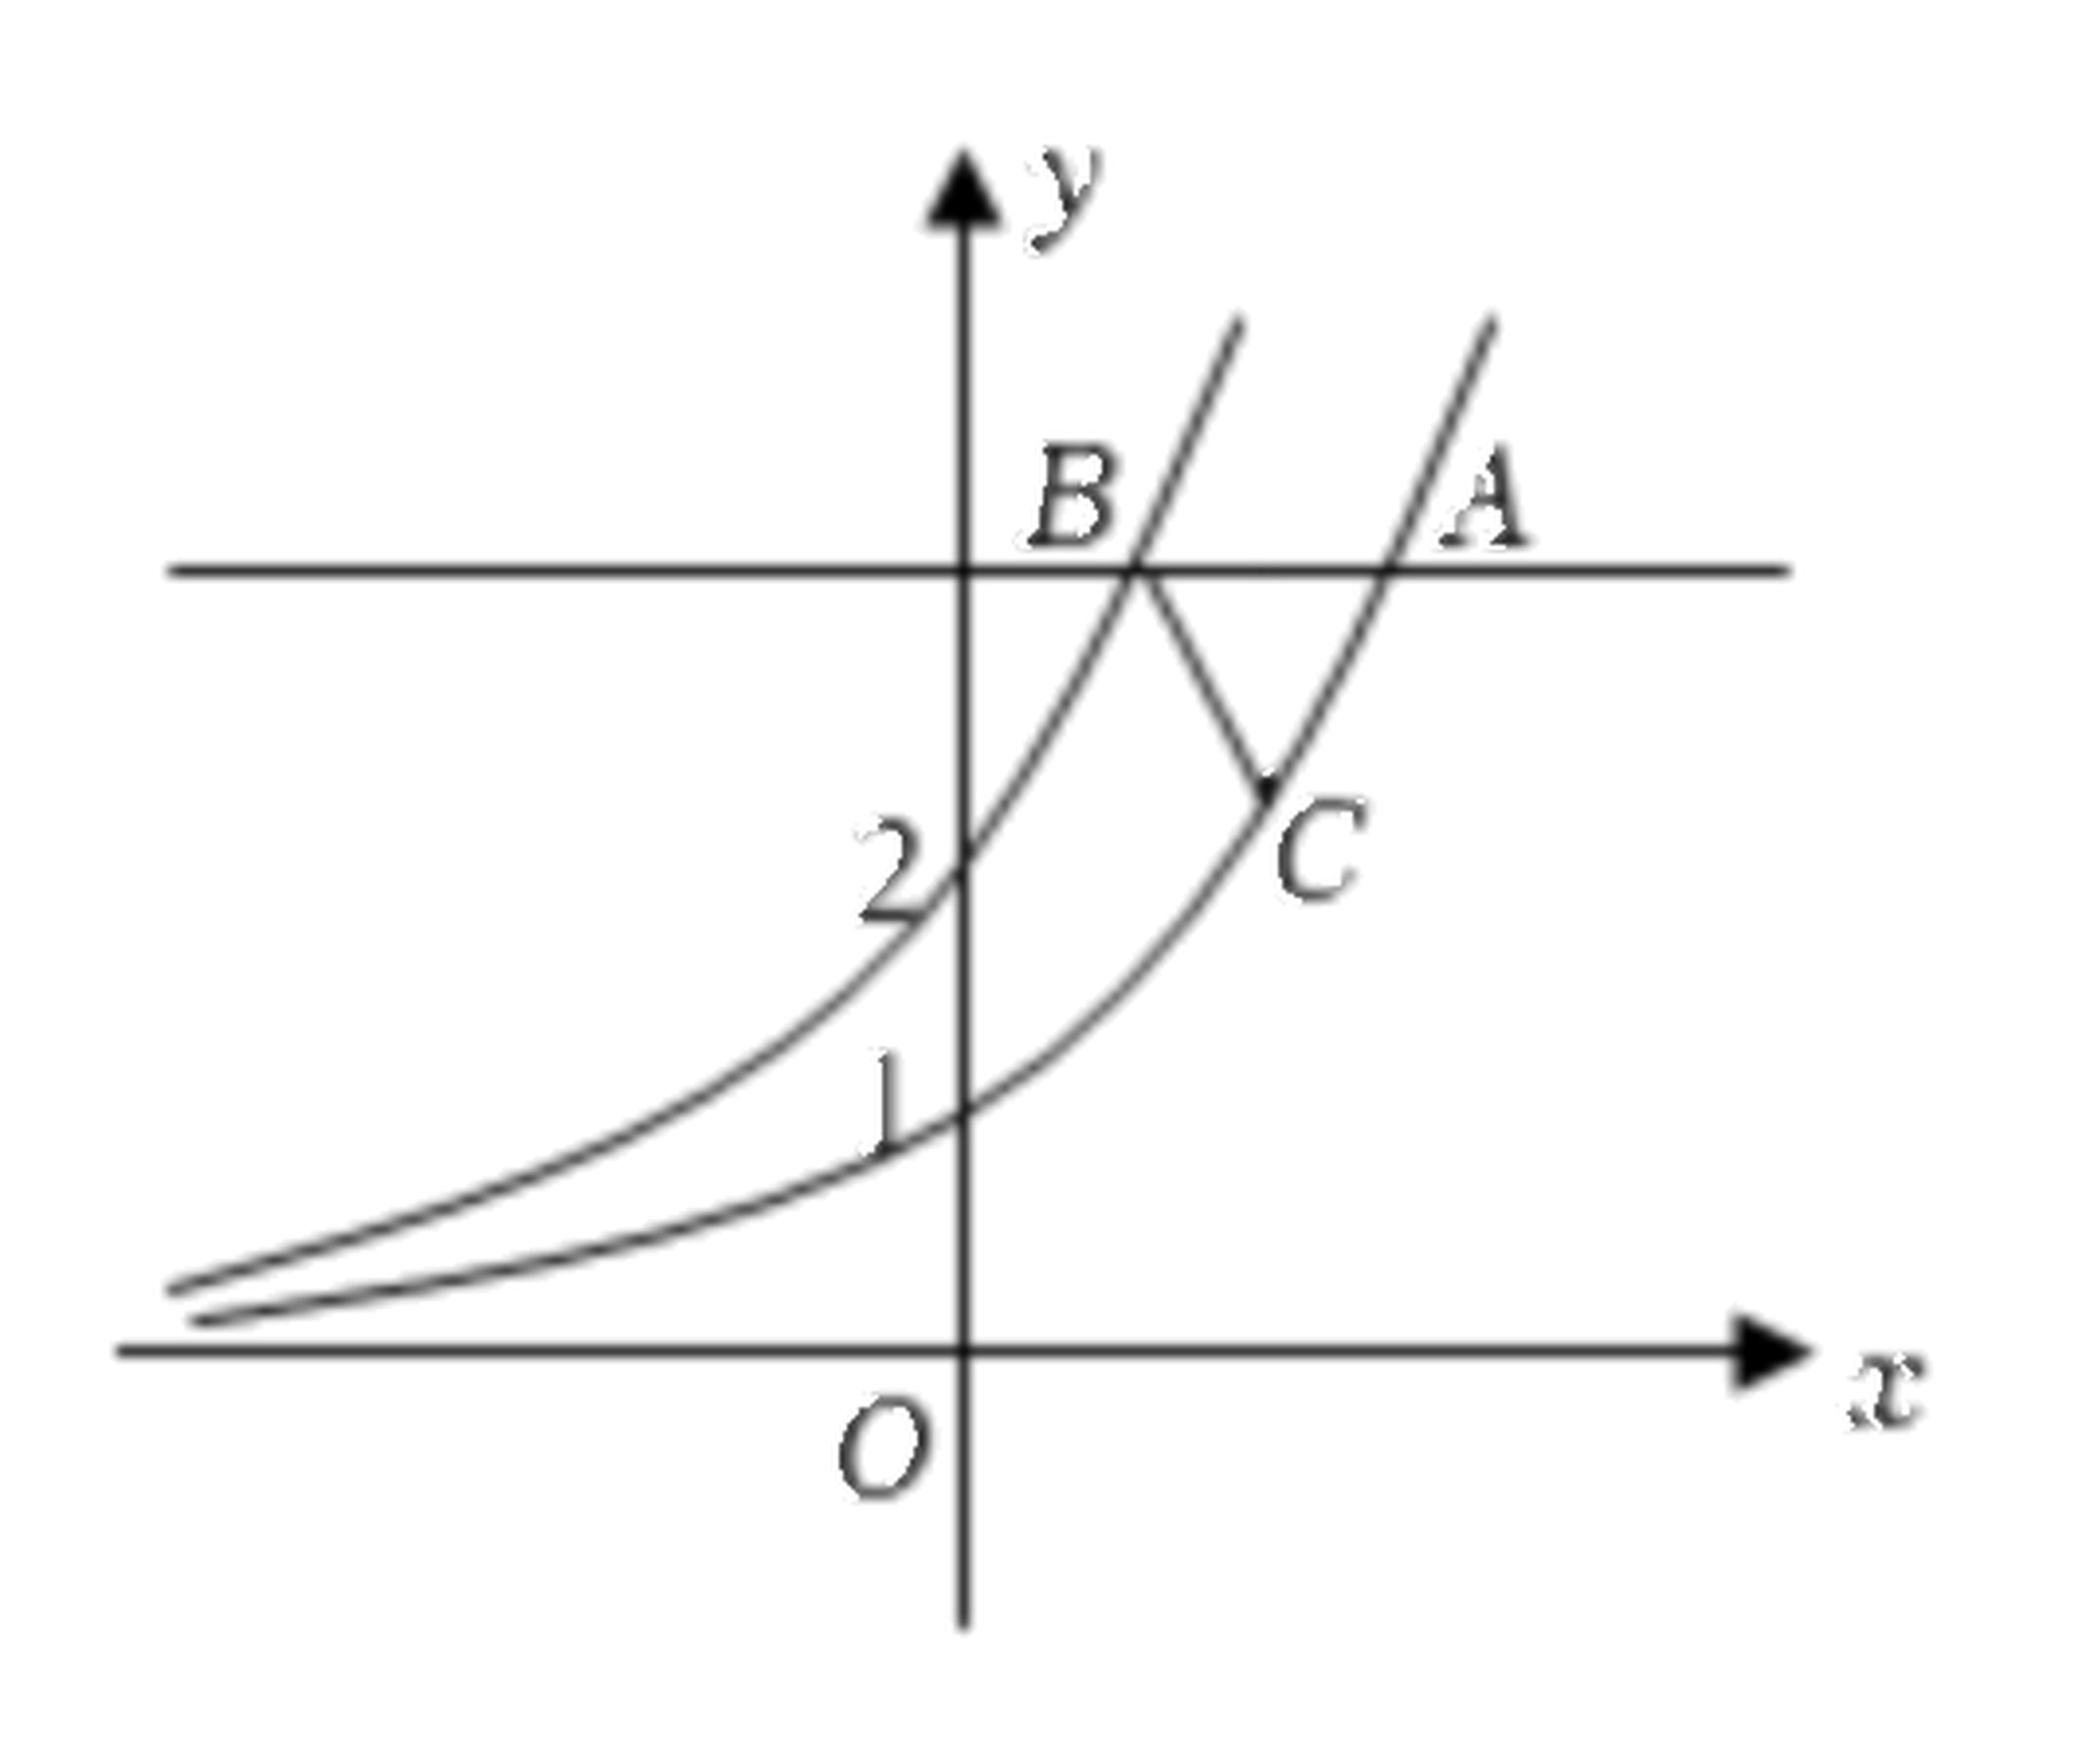
\includegraphics[width=0.40\textwidth]{figures/gao150_q11.png}
\end{center}

\ifanswer
\solbegin
\step{设直线 $l$ 的方程为 $y=a(a>0)$，}
\step{由 $2^x=a$，得 $x=\log_2 a$，所以 $A(\log_2 a,a)$，}
\step{由 $2^{x+1}=a$，得 $x=\log_2 a-1$，所以 $B(\log_2 a-1,a)$，所以 $\lvert AB\rvert=1$，}
\step{取 $AB$ 的中点 $D$，连接 $CD$，如图所示，}
\step{因为 $\triangle ABC$ 为等边三角形，则 $CD\perp AB$，且 $\lvert CD\rvert=\dfrac{\sqrt3}{2}$，}
\step{所以 $C\left(\log_2 a-\dfrac{1}{2},a-\dfrac{\sqrt3}{2}\right)$，}
\step{因为点 $C$ 在函数 $y=2^x$ 的图像上，所以 $a-\dfrac{\sqrt3}{2}=2^{\log_2 a-\frac{1}{2}}=\dfrac{a}{\sqrt2}$，}
\step{解得 $a=\dfrac{\sqrt3}{2-\sqrt2}=\dfrac{\sqrt3(2+\sqrt2)}{4-2}=\sqrt3+\dfrac{\sqrt6}{2}$，}
\step{所以点 $C$ 的纵坐标为 $a-\dfrac{\sqrt3}{2}=\dfrac{\sqrt3+\sqrt6}{2}$.}
\solend
\fi

% === Q12 === 解析配图（高斯函数方格阴影，仅答案版出）；"数学王子"弯引号；cases 块整体算一个印刷行；解析 4 行
\item 小玲在研究数学发展史，特别崇拜近代数学奠基者之一、享有“数学王子”称号的德国数学家高斯. 为了纪念高斯，我们把取整函数 $y=[x]$ 称为高斯函数，其中 $[x]$ 表示不超过 $x$ 的最大整数，如 $[1.1]=1$，$[-1.1]=-2$，则点集 $P=\{(x,y)\mid [x]^2+[y]^2=1\}$ 所表示的平面区域的面积为\blankline[4.4em].

\ifanswer
\solbegin
\step{$[x]^2+[y]^2=1$ 由 $\begin{cases}[x]=0\\ {[y]=-1}\end{cases}$ 或 $\begin{cases}[x]=0\\ {[y]=1}\end{cases}$ 或 $\begin{cases}[x]=-1\\ {[y]=0}\end{cases}$ 或 $\begin{cases}[x]=1\\ {[y]=0}\end{cases}$ 四个平面区域组成，}
\step{即 $\begin{cases}0\leqslant x<1\\ -1\leqslant y<0\end{cases}$ 或 $\begin{cases}0\leqslant x<1\\ 1\leqslant y<2\end{cases}$ 或 $\begin{cases}-1\leqslant x<0\\ 0\leqslant y<1\end{cases}$ 或 $\begin{cases}1\leqslant x<2\\ 0\leqslant y<1\end{cases}$，}
\step{作出平面区域如图所示，平面区域由四个边长为 $1$ 的正方形组成，}
\begin{center}
% 高斯函数 [x]^2+[y]^2=1 方格阴影区域图取 04 页顶部，去粉色水印、去色、4× LANCZOS 放大；仅答案版出
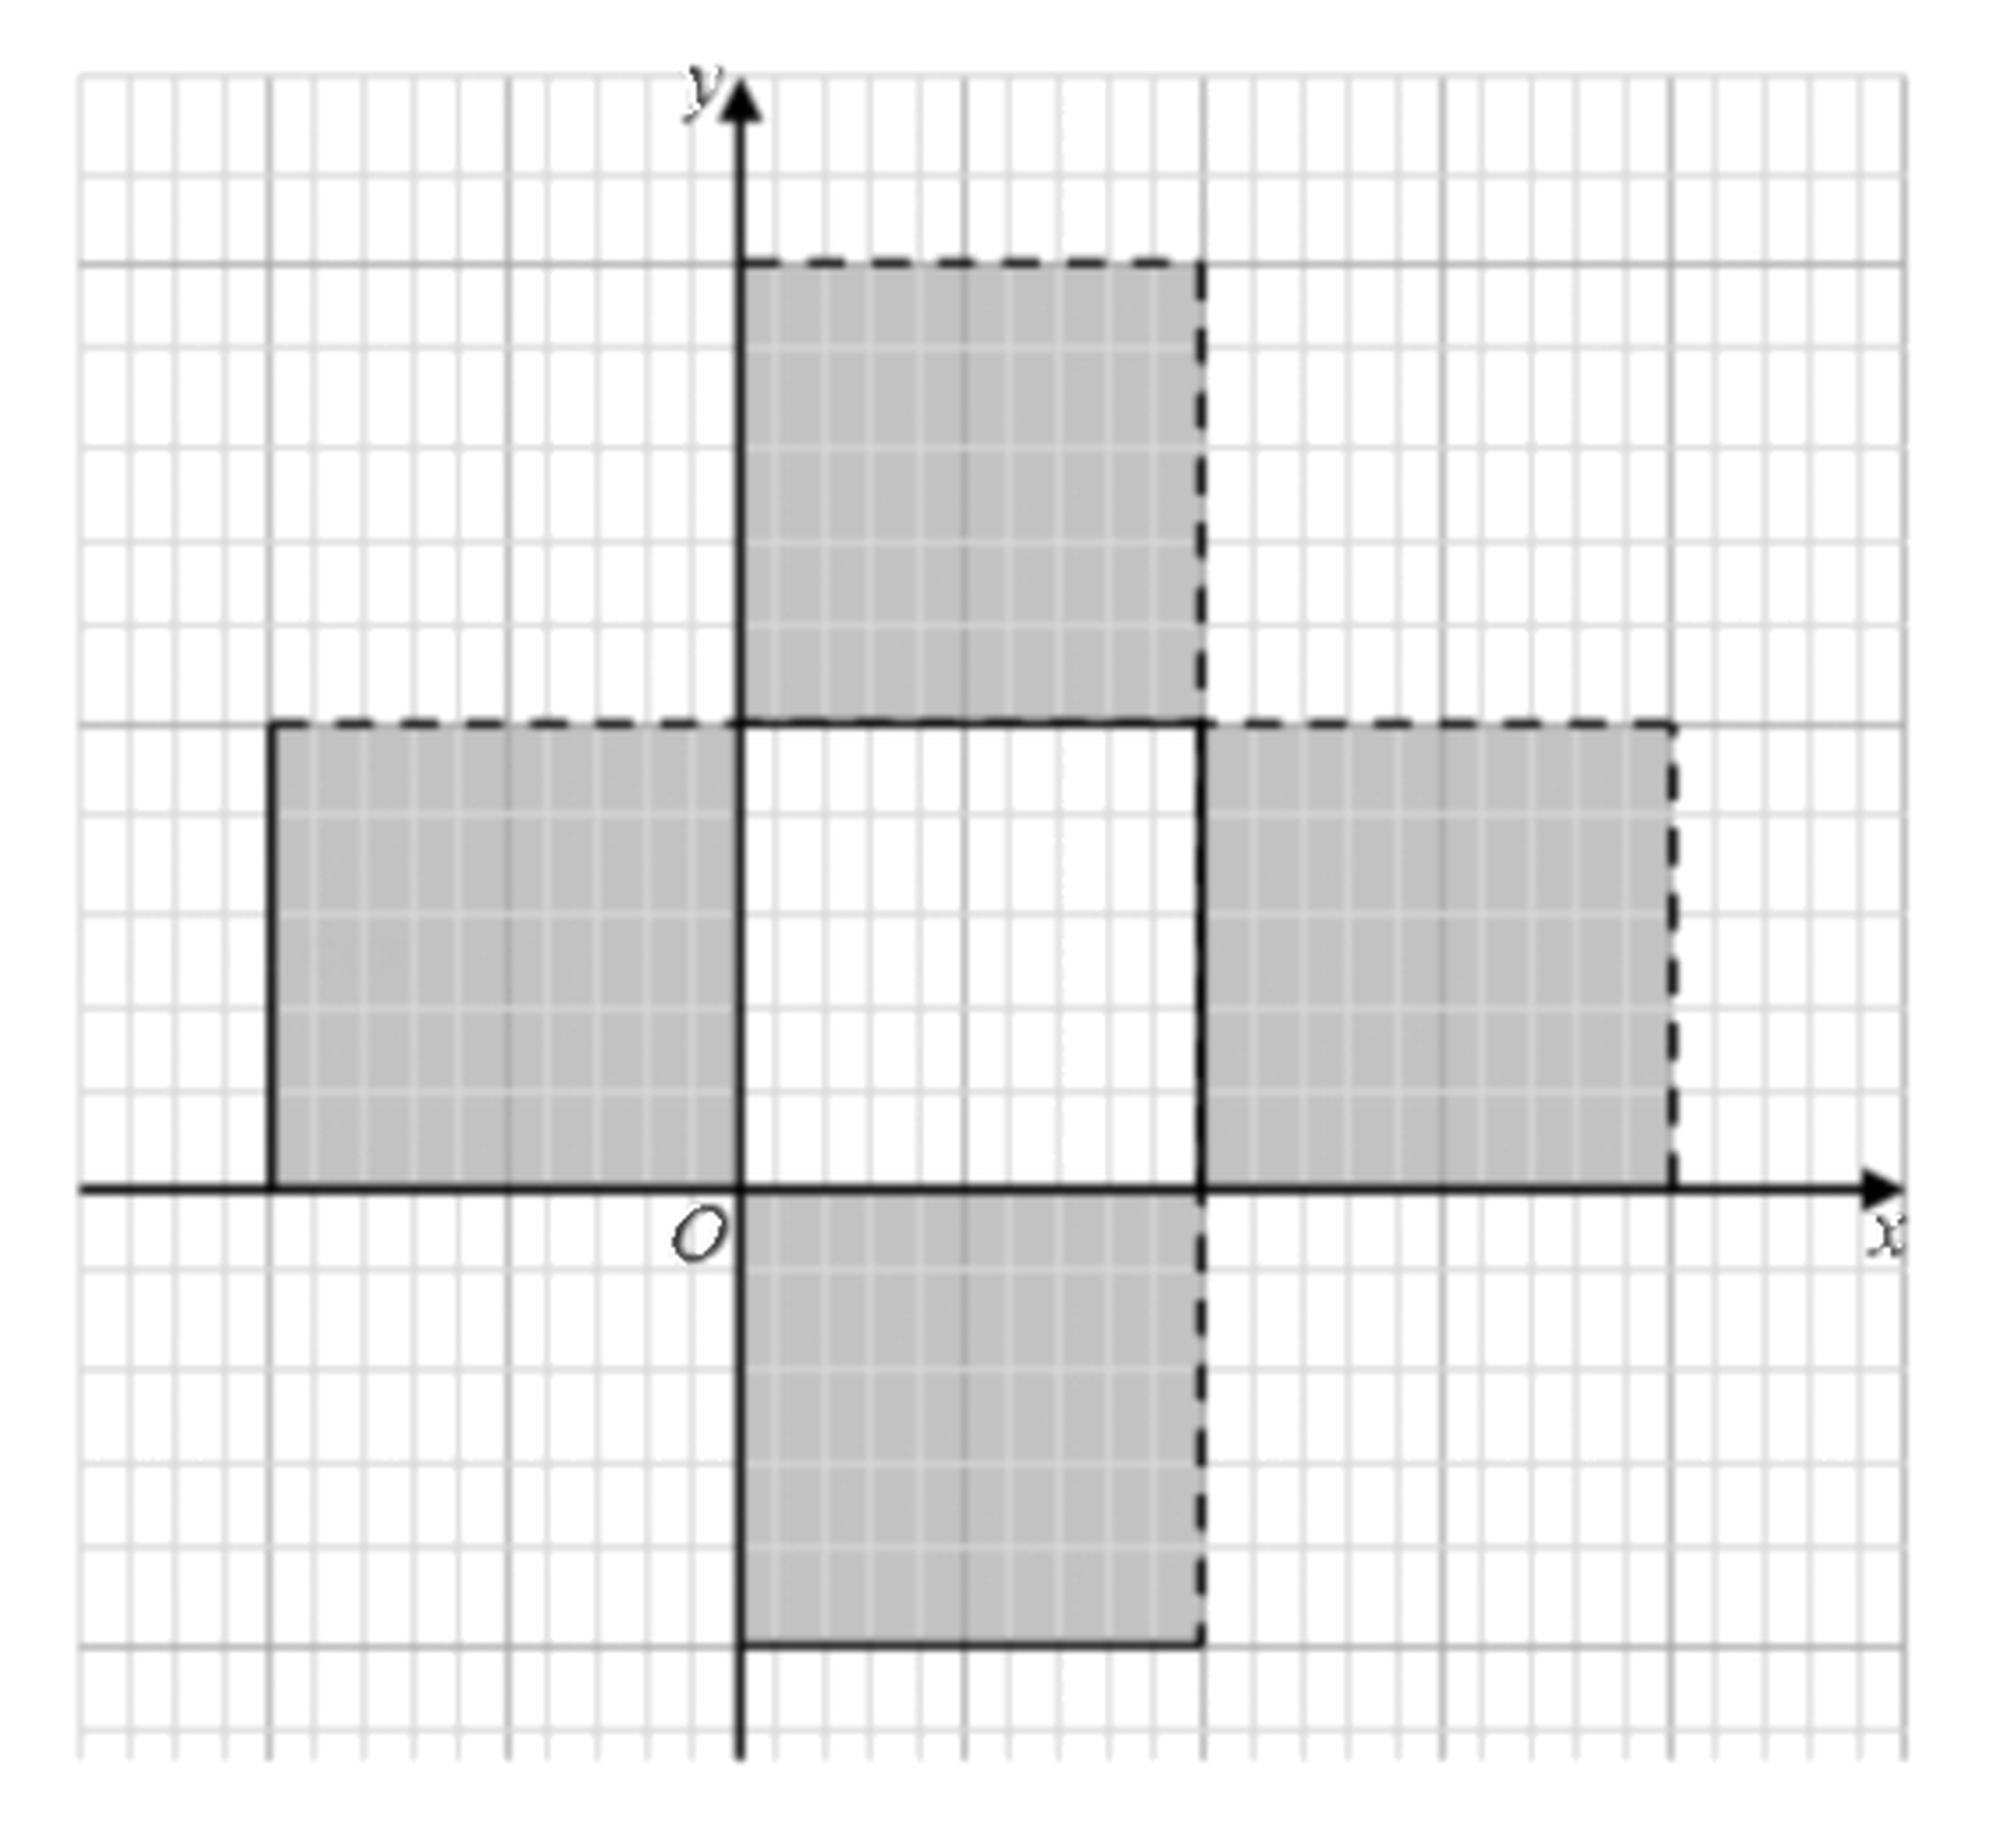
\includegraphics[width=0.34\textwidth]{figures/gao150_q12.png}
\end{center}
\step{总面积为 $1\times4=4$.}
\solend
\fi

\end{enumerate}

\bigsec{二、选择题}

\begin{enumerate}
\setcounter{enumi}{12}

% === Q13 === 答案在解析末句"故选 C"；括号 \mbox{（\quad）} 留空；四选项一行；解析 1 行
\item 设 $x\ne0$，则 $3^{\log_9 x^2}$ 的化简结果是\mbox{（\quad）}

\keepwithprev
A. $x$\qquad B. $\dfrac{1}{x}$\qquad C. $\lvert x\rvert$\qquad D. $\dfrac{1}{\lvert x\rvert}$

\ifanswer
\solbegin
\step{$3^{\log_9 x^2}=3^{\log_3\lvert x\rvert}=\lvert x\rvert$，故选 $C$.}
\solend
\fi

% === Q14 === 题目配图（两函数图像，三版都出）；\needvspace{8cm} 守卫放 \item 之前；"图像"照录；四选项两行两列；解析 2 行，故选 B
\needvspace{8cm}
\item 设 $a>0$ 且 $a\ne1$，$b\in\R$. 若函数 $y=a^{-\lvert x\rvert}$ 与 $y=x^b$ 的大致图像如图所示，则\mbox{（\quad）}

\keepwithprev
A. $0<a<1<b$\qquad\qquad B. $a>1$ 且 $b>1$

C. $0<a<1$ 且 $0<b<1$\qquad\qquad D. $0<b<1<a$

\begin{center}
% 两函数 y=a^{-|x|} 与 y=x^b 大致图像取 04 页右侧，去粉色水印、去色、4× LANCZOS 放大；三版都出
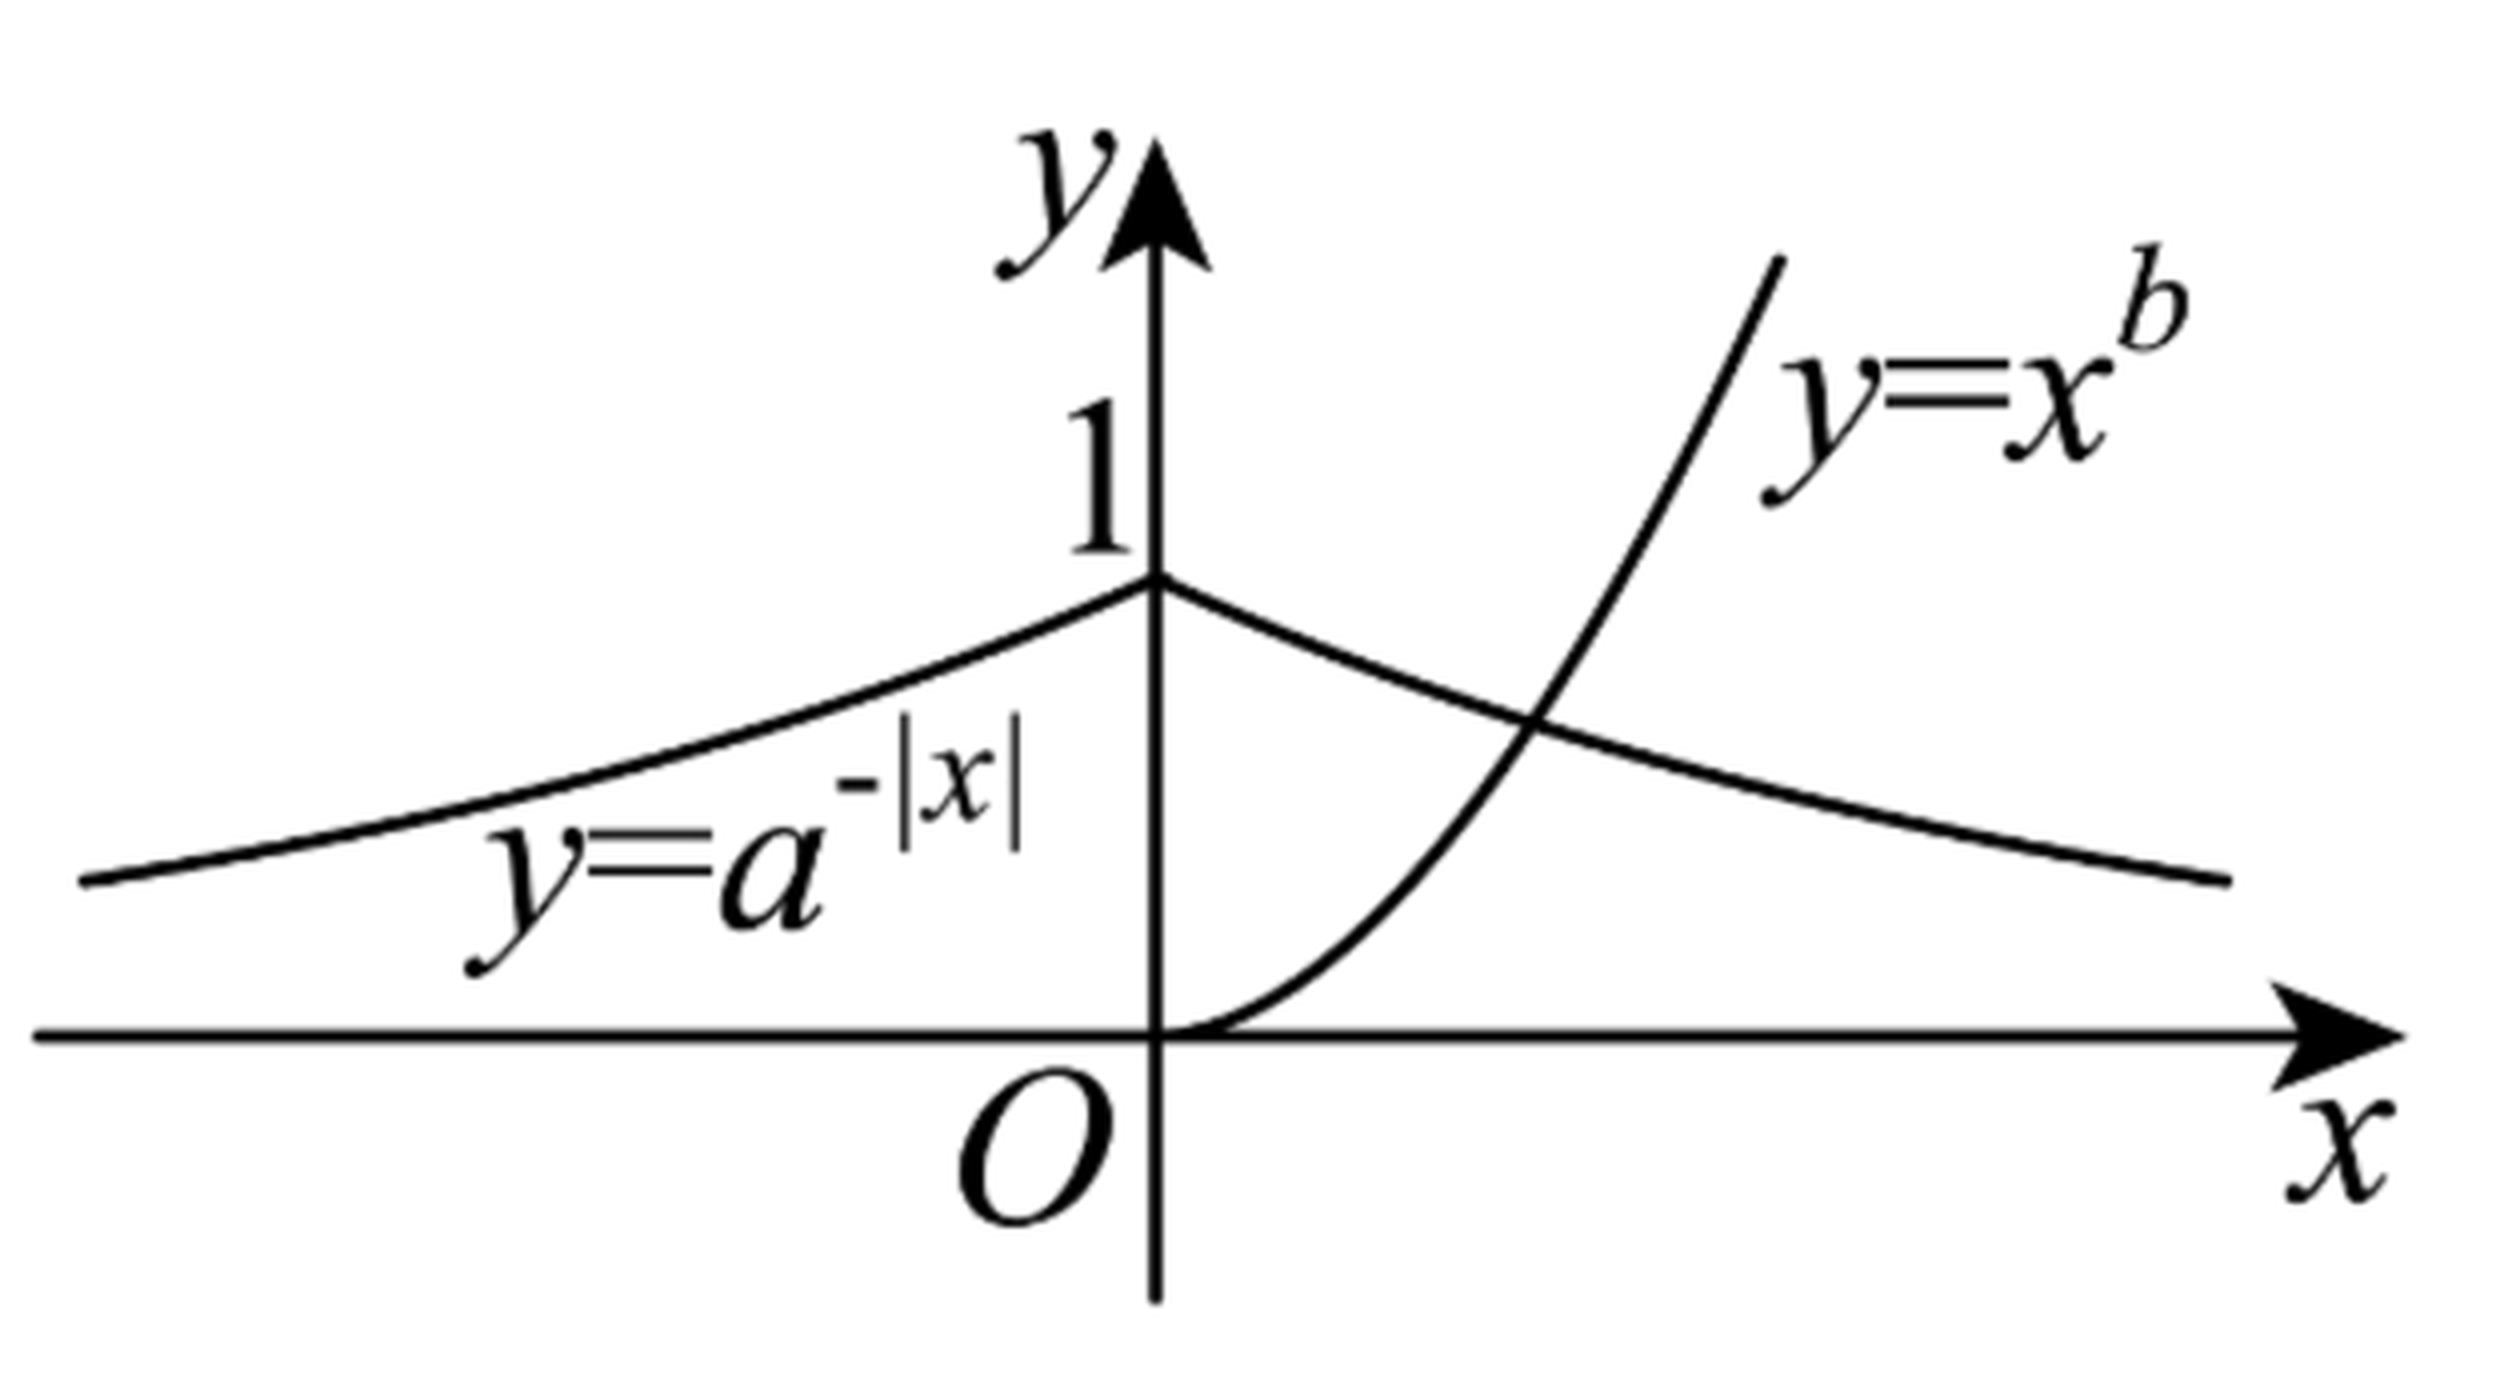
\includegraphics[width=0.40\textwidth]{figures/gao150_q14.png}
\end{center}

\ifanswer
\solbegin
\step{在 $(0,+\infty)$ 上，$y=a^{-x}$ 严格递减，得 $a>1$；}
\step{幂函数 $y=x^b$ 的图像递增且向上弯曲，得 $b>1$；故选 $B$.}
\solend
\fi

% === Q15 === "算术平均值／算术平均数"两处不同照录；四选项两行两列；解析 5 行（续 05 页顶），故选 B
\item 已知两个正数的算术平均值不小于它们的几何平均值，类比有以下结论：三个正数的算术平均数不小于它们的几何平均数，即当 $a,b,c$ 为正实数时，$\dfrac{a+b+c}{3}\geqslant\sqrt[3]{abc}$，当且仅当 $a=b=c$ 时等号成立. 利用上述结论，下列选项中判断正确的是\mbox{（\quad）}

\keepwithprev
A. 若 $x>0$，则 $2x+\dfrac{1}{x^2}\geqslant\dfrac{27}{8}$\qquad\qquad B. 若 $x>0$，则 $x^2+\dfrac{2}{x}\geqslant3$

C. 若 $0<x<1$，则 $x^2(1-x)\geqslant\dfrac{1}{9}$\qquad\qquad D. 若 $0<x<1$，则 $x^2(1-x)\leqslant\dfrac{1}{9}$

\ifanswer
\solbegin
\step{A：取 $x=1$，$2x+\dfrac{1}{x^2}=3<\dfrac{27}{8}$，错误.}
\step{B：$x^2+\dfrac{2}{x}=x^2+\dfrac{1}{x}+\dfrac{1}{x}\geqslant3\sqrt[3]{x^2\cdot\dfrac{1}{x}\cdot\dfrac{1}{x}}=3$，当且仅当 $x=1$ 时取等号，正确.}
\step{C：取 $x=\dfrac{1}{3}$，$x^2(1-x)=\dfrac{2}{27}<\dfrac{1}{9}$，错误.}
\step{D：取 $x=\dfrac{2}{3}$，$x^2(1-x)=\dfrac{4}{27}>\dfrac{1}{9}$，错误.}
\step{故选 $B$.}
\solend
\fi

% === Q16 === "完美集"新定义（弯引号、引号外空格照录）；圈数字①②文本模式；$n\in\N$；四选项两行两列；解析 9 行（6 行 05 页＋3 行 06 页顶），故选 A
\item 已知有限集 $A=\{a_1,a_2,\cdots,a_n\}$（$n\geqslant2$，$n\in\N$）. 若 $A$ 中元素 $a_i$（$i=1,2,\cdots,n$）满足 $a_1+a_2+\cdots+a_n=a_1\cdot a_2\cdots a_n$，就称 $A$ 为 “完美集”. 现有以下两个命题：

①恰有两个元素的 “完美集” 有无穷多个；

②若 $a_i$ 均为正整数，则 “完美集” $A$ 有且只有一个，且 $n=3$.

则\mbox{（\quad）}

\keepwithprev
A. ①和②都是真命题\qquad\qquad B. ①和②都是假命题

C. ①是真命题，②是假命题\qquad\qquad D. ①是假命题，②是真命题

\ifanswer
\solbegin
\step{①由 $a+b=ab\Leftrightarrow(a-1)(b-1)=1$，任取 $a>2$，则 $b=1+\dfrac{1}{a-1}\in(1,2)$，}
\step{得到无穷多个不同的完美集，①真.}
\step{②设 $1\leqslant a_1<a_2<\cdots<a_n$，则 $a_i\geqslant i$.}
\step{若 $n=2$，则 $(a_1-1)(a_2-1)=1$，只能有 $a_1=a_2=2$，与元素互异矛盾.}
\step{若 $n\geqslant4$，则 $a_1a_2\cdots a_n\geqslant a_2a_{n-1}a_n\geqslant2(n-1)a_n>na_n\geqslant a_1+\cdots+a_n$，矛盾.}
\step{当 $n=3$ 时，若 $a_1\geqslant2$，则 $a_1a_2a_3\geqslant6a_3>3a_3\geqslant a_1+a_2+a_3$，矛盾.}
\step{因此 $a_1=1$，$(a_2-1)(a_3-1)=2$，结合 $a_2<a_3$ 得 $a_2=2$，$a_3=3$.}
\step{唯一的完美集为 $\{1,2,3\}$，②真.}
\step{故选 $A$.}
\solend
\fi

\end{enumerate}

\bigsec{三、解答题}

\begin{enumerate}
\setcounter{enumi}{16}

% === Q17 === \varnothing 空集、$B\subseteq A$ 带下划线照录；弯引号内空格照录；解析 7 行
\item 设 $a,b\in\R$. 已知集合 $A=\{x\mid ax^2+3x-a>3\}$，$B=\{x\mid bx=1\}$.

(1) 若 $A=(1,2)$，求 $a$ 的值；

(2) 若 $a=0$，且 “ $x\in A$ ” 是 “ $x\in B$ ” 的必要非充分条件，求 $b$ 的取值范围.

\ifanswer
\solbegin
\step{(1) $A=(1,2)$，则 $a<0$，且 $1,2$ 是方程 $ax^2+3x-a-3=0$ 的两根.}
\step{由 $4a+6-a-3=0$，得 $a=-1$，此时不等式为 $-(x-1)(x-2)>0$，}
\step{解集确为 $(1,2)$.}
\step{(2) $a=0$ 时，$A=(1,+\infty)$，题意等价于 $B\subseteq A$ 且 $B\ne A$.}
\step{当 $b=0$ 时，$B=\varnothing$，符合条件.}
\step{当 $b\ne0$ 时，$B=\left\{\dfrac{1}{b}\right\}$，条件等价于 $\dfrac{1}{b}>1$，解得 $0<b<1$.}
\step{因此 $b$ 的取值范围为 $[0,1)$.}
\solend
\fi

% === Q18 === $p\in\Z$；"图像"（像，有亻）照录；指数 $-2p^2+5p$；解析 8 行（(1) 首行 06 页末＋2 行 07 页顶、(2) 5 行 07 页）
\item 设 $p\in\Z$，已知 $f(x)=x^{-2p^2+5p}$.

(1) 若幂函数 $y=f(x)$ 的图像关于原点成中心对称，且满足 $f(3)<f(4)$，求 $p$ 的值；

(2) 当 $p=-2$ 时，求满足 $f(2x+3)<f(x-4)$ 的 $x$ 的取值范围.

\ifanswer
\solbegin
\step{(1) 图像关于原点成中心对称，得整数 $-2p^2+5p$ 为奇数.}
\step{由 $f(3)<f(4)$，得 $-2p^2+5p>0\Leftrightarrow0<p<\dfrac{5}{2}$，}
\step{结合 $p\in\Z$，得 $p=1$ 或 $p=2$，对应指数分别为 $3$、$2$，所以 $p=1$.}
\step{(2) 当 $p=-2$ 时，$f(x)=\dfrac{1}{x^{18}}$，定义域为 $\{x\in\R\mid x\ne0\}$.}
\step{原不等式要求 $x\ne-\dfrac{3}{2}$ 且 $x\ne4$，}
\step{此时 $\dfrac{1}{(2x+3)^{18}}<\dfrac{1}{(x-4)^{18}}\Leftrightarrow\lvert 2x+3\rvert>\lvert x-4\rvert\Leftrightarrow(2x+3)^2>(x-4)^2$，}
\step{因此 $(x+7)(3x-1)>0\Leftrightarrow x<-7$ 或 $x>\dfrac{1}{3}$，}
\step{排除 $x=4$，得 $x\in(-\infty,-7)\cup\left(\dfrac{1}{3},4\right)\cup(4,+\infty)$.}
\solend
\fi

% === Q19 === $a\in\R$、$g(x)=f(2x+1)+a\cdot f(x)+2$；解析 6 行（(2) 末两行续 08 页顶）
\item 已知 $f(x)=2^x$.

(1) 求方程 $f(2x)-f(x)=6$ 的解；

(2) 设 $a\in\R$，$g(x)=f(2x+1)+a\cdot f(x)+2$，若对于任意 $x\in[-1,1]$，均有 $g(x)\geqslant1$，求 $a$ 的取值范围.

\ifanswer
\solbegin
\step{(1) 令 $t=2^x>0$，则 $t^2-t-6=(t-3)(t+2)=0$，}
\step{由 $t>0$ 得 $t=3$，所以 $x=\log_2 3$.}
\step{(2) 令 $t=2^x$，则 $t\in\left[\dfrac{1}{2},2\right]$，且 $g(x)\geqslant1\Leftrightarrow2t^2+at+1\geqslant0\Leftrightarrow a\geqslant-\left(2t+\dfrac{1}{t}\right)$，}
\step{由基本不等式得 $2t+\dfrac{1}{t}\geqslant2\sqrt{2t\cdot\dfrac{1}{t}}=2\sqrt2$，}
\step{当且仅当 $t=\dfrac{1}{\sqrt2}\in\left[\dfrac{1}{2},2\right]$ 时等号成立，}
\step{因此 $-\left(2t+\dfrac{1}{t}\right)$ 的最大值为 $-2\sqrt2$，所求范围为 $a\in[-2\sqrt2,+\infty)$.}
\solend
\fi

% === Q20 === "极闭集"新定义、3 问，全卷末题；$M\subseteq(0,+\infty)$ 带下划线照录；自定义运算 $x*y$ 星号照录；解析 13 行（9 行 08 页＋4 行 09 页上半）
\item 对于非空实数集 $M\subseteq(0,+\infty)$，若满足以下两个条件：

① $M$ 中至少含有 $2$ 个元素，且 $1\notin M$；

②对于 $M$ 中任意两个不相等的元素 $x$、$y$，定义 $x*y=\dfrac{xy+1}{x+y}$，且 $x*y\in M$.

则称 $M$ 为 “极闭集”.

(1) 分别判断集合 $A=\left\{\dfrac{1}{2},3\right\}$ 与集合 $B=(1,+\infty)$ 是否为 “极闭集” （无需理由）；

(2) 若 $M$ 是 “极闭集”，证明：$M$ 中不可能所有元素都小于 $1$；

(3) 证明：不存在任何有限集是 “极闭集”.

\ifanswer
\solbegin
\step{(1) $A$ 不是 “极闭集”，$B$ 是 “极闭集”.}
\step{(2) 假设 $M$ 中所有元素都小于 $1$，取其中两个不相等的元素 $x$、$y$，}
\step{则 $x*y-1=\dfrac{(1-x)(1-y)}{x+y}>0$，}
\step{这与 $x*y\in M$ 且 $M$ 中所有元素都小于 $1$ 矛盾.}
\step{(3) 假设有限集 $M$ 是 “极闭集”，}
\step{由 (2) 及 $1\notin M$，得 $M$ 中存在大于 $1$ 的元素.}
\step{若 $M$ 中有小于 $1$ 的元素，取其中最大的一个为 $a$，另取 $b\in M$ 且 $b>1$，}
\step{则 $a*b-a=\dfrac{1-a^2}{a+b}>0, a*b-1=\dfrac{(a-1)(b-1)}{a+b}<0$，}% 半角逗号在两个数学式组之间，全稿惯例、非笔误，照录
\step{于是 $a<a*b<1$ 且 $a*b\in M$，与 $a$ 的最大性矛盾.}
\step{若 $M$ 中没有小于 $1$ 的元素，则 $M\subseteq(1,+\infty)$.}
\step{取 $a=\min M$，另取 $b\in M$ 且 $b\ne a$，则 $a*b-a=\dfrac{1-a^2}{a+b}<0$，}
\step{于是 $a*b<a$ 且 $a*b\in M$，与 $a$ 的最小性矛盾.}
\step{因此不存在任何有限集是 “极闭集”.}
\solend
\fi

\end{enumerate}

\end{document}
"
% 紧凑版：xelatex "\def\iscompact{1}% 高一150_曹杨二中_期中.tex
%   —— 高一上数学"2026-2027 年曹杨二中高一上期中"（试卷版/答案版/紧凑版）
% 试卷版：xelatex 高一150_曹杨二中_期中.tex
% 答案版：xelatex "\def\isanswer{1}\input{高一150_曹杨二中_期中.tex}"
% 紧凑版：xelatex "\def\iscompact{1}\input{高一150_曹杨二中_期中.tex}"
%
% ① 原始材料：微信公众号"魔都数学加油站"文章，连载"27学年高一150"，原文标题
% "27学年高一150——2026-2027年上海市曹杨二中高一上期中"；
% 原文链接：https://mp.weixin.qq.com/s/xlQxmik8TZXR87RC6MnCrw 。
% 正文为 9 张 PNG 页（01/02/04/06/07/09 为 2560×3620，03/05/08 为 4762×6735，
% 同一篇各页分辨率混排，逐页按各自分辨率裁图核对，别按预览比例换算裁框）。
% 体例：讲评版——全 18 题均印【解析】（逐题核实，见 ② ②）。
% 题目、答案、解析均据原图转录；卷面粉红色/红色水印"魔都数学加油站"及公众号页脚未录入。
% 全卷插图清单（逐页通读 9 页确认）：3 幅——
%   · Q11 题目配图（指数函数曲线图，02 页右侧：x/y 轴、O、y=2^x 与 y=2^{x+1}
%     两曲线、A/B/C 三点、刻度 1/2、等边三角形 ABC），三版都出，裁 figures/gao150_q11.png；
%   · Q12 解析配图（高斯函数取整 [x]^2+[y]^2=1 方格阴影区域图，04 页顶部：4 个边长 1
%     的正方形组成的十字形阴影），解析"作出平面区域如图所示"处，仅答案版出，
%     放 \ifanswer 内 \step 之间，裁 figures/gao150_q12.png；
%   · Q14 题目配图（两函数 y=a^{-|x|} 与 y=x^b 大致图像，04 页右侧：x/y 轴、O、
%     y 轴刻度 1、一递减曲线一递增上翘曲线），三版都出，裁 figures/gao150_q14.png；
%   其余各页逐页确认无其它题目配图、无表格；Q11/Q12 解析"如图所示"对应的就是上列
%   已裁的图，不重复裁；09 页上半为 Q20(3) 解析续尾、下半仅水印、无正文。
%   3 图均取自原卷截图，去粉色水印、去色、4× LANCZOS 放大。
%
% 卷首标题：原卷印作"2026-2027 年曹杨二中高一上期中"，年份区间按全稿惯例排 en dash；
% 原卷卷面未印副标题，本稿按同期中卷知识模块口径补出"集合与常用逻辑用语、不等式、函数"。
%
% 题号体例（逐页核实定稿）：本卷共 18 题——一、填空题 3—12（10 题）、
% 二、选择题 13—16（4 题）、三、解答题 17—20（4 题）。
% 三节分别 \setcounter{enumi}{2}／{12}／{16}。原卷从第 3 题起、无第 1、2 题，
% 本稿保留原题号；全卷末题为第 20 题（"极闭集"新定义、3 问），无 Q21、无附加题节。
%
% ② 与原卷的排版差异：
%   ① 原文从第 3 题起，本稿保留原题号；共 18 题三节，解答题只有 4 题到 20；
%   ② 全 18 题均印【解析】，用 \solbegin…\solend；逐题核实无只印【答案】或
%      答案印题干括号内的题；四道选择题答案在解析末句"故选 X"（Q13 选 C、
%      Q14 选 B、Q15 选 B、Q16 选 A，逐个放大复核）、括号 \mbox{（\quad）} 留空、
%      不另提 \ans{}；答案版【答案】/【解析】标记数 = 18 = 全卷题数；
%   ③ 原卷卷面未印副标题，本稿按知识模块口径补出；
%   ④ 原卷填空横线按全稿惯例排 \blankline[4.4em]；选择题括号排 \mbox{（\quad）}、
%      选项段前按惯例加 \keepwithprev；解答题不留作答区、不加 \anspace（原卷为讲评版）；
%   ⑤ 数集黑板粗体：Q4"m\in R"、Q5"a,b\in R"、Q6"a,b,c\in R"、Q7"a\in R"、
%      Q10"a\in R"、Q14"b\in R"、Q17"a,b\in R"、Q18"p\in Z"／定义域"x\in R"、
%      Q19"a\in R"、Q16"n\in N" 原卷印斜体 R/Z/N，按全稿惯例归一 \R／\Z／\N；
%      绝对值排 \lvert…\rvert（Q7 |x+4|+|x-3|、Q11 |AB|／|CD|、Q13 |x|、
%      Q18 |2x+3|／|x-4|），集合描述竖线排 \mid（Q3、Q12、Q17、Q18、Q20），
%      不等号按全稿惯例排 \leqslant／\geqslant；补集照原卷上划线排 \overline{A}
%      （Q3 题干＋解析共 2 处）；空集符号 \varnothing（Q17 解析(2)）；
%      子集 \subset（单线⊂）／\subseteq（带下划线⊆）逐处照录，本卷 3 处子集
%      符号均印带下划线 ⊆、照录 \subseteq（Q20 题干、Q20 解析(3)、Q17 解析(2)，
%      见 ④），无 \subset 用例；
%   ⑥ 判别式 Δ/△：逐页通读 9 页，本卷无一元二次判别式算式，故无 Δ/△ 混用可照录
%      （"高 \Delta／扁 \triangle"口径备查，参照 高一142／144／145／146／148／149
%      头注④）；本卷仅 Q11 题干与解析共 2 处几何三角形符号 △ABC，逐处放大并排
%      确认两处同形、印近等边粗线三角（非判别式），照录 \triangle（见 ④）；
%   ⑦ 中文弯引号照录：Q12"数学王子"、Q16"完美集"（题干＋①②两命题，引号外
%      留空格）、Q17" x∈A "" x∈B "（引号内空格）、Q20"极闭集"（题干条件、
%      三问与解析，引号外留空格）；注释里一律 ASCII 引号；数学式内 CJK 用 \text{}
%      （Q3 集合描述"且"用 \text{ 且 }）；
%   ⑧ 半角逗号在数学组之间是全稿惯例、非笔误，逐处照录（Q17 解析"1,2 是方程…
%      两根"、Q20 解析(3)">0, a*b-1=…<0" 两式之间等）；行末西文句点 ASCII `.`；
%      行中全角逗号／顿号照录（Q12"之一、享有"、Q18 解析"3、2"、Q20"x、y"）；
%   ⑨ "图像／图象"逐处放大核：全卷 9 处均印"图像"（像，有亻）、未见"图象"——
%      Q4 题干 1、Q11 题干 2＋解析 1、Q14 题干 1＋解析 1、Q18 题干 1＋解析 1；
%      同卷"第二象限""象限"用"象"（无亻）。逐处照录未统一改动（放大 01/02/04/06
%      页 /tmp/gao150/z/p01_q4_tuxiang2.png、p04_q14_tuxiang2.png、
%      p02_q11_lines.png 确认）；子题标号 (1)(2)(3) 半角括号照录；圈数字①②
%      在文本模式（Q16 两命题与解析、Q20 两条件与三问及解析）按 common.sty
%      划入 CJK 字符类渲染，进数学式用 \text{①}；
%   ⑩ Q20 新定义 x*y=\dfrac{xy+1}{x+y} 的 * 是自定义运算（星号），照录；
%      \left…\right 不得拆到不同 $…$ 组（Q19"\left(2t+\frac1t\right)"、
%      Q20 题干"A=\left\{\frac12,3\right\}"等）；Q8 嵌套根号
%      \sqrt{\frac2x+\frac{16}{1-2x}}、Q9 对数连加 \log_2 A 等复杂式照录别简化；
%   ⑪ 一条 \step = 原卷解析的一个印刷行，cases 块整体算一个印刷行；别并折行、
%      别拆行。Q4 三行、Q8 五行、Q11 九行、Q12 四行（两行各含四个 cases 块）、
%      Q15 五行、Q16 九行、Q18 八行、Q20 十三行均按印刷行逐条断，不丢行；
%   ⑫ 配图：Q11／Q14 题目配图（三版都出）放 \item 内题干之后 \begin{center}，
%      大图块加 \needvspace{8cm} 守卫把整块推走（守卫放 \item 之前，见
%      高一145 Q14/Q20 成例与切页审计 B 类坑）；Q12 解析配图（仅答案版出）
%      放 \ifanswer 内 \solbegin…\solend 的 \step 之间（高一73 第16题成例）；
%   ⑬ 跨页续印按题合并：见 ⑥；
%   ⑭ 原卷解析内无红色"法一／法二"之类小标题，故本卷无 \stepm；红色水印
%      "魔都数学加油站"不录入；Q12 解析"作出平面区域如图所示"对应的图即
%      ① 所列 gao150_q12.png（04 页顶部），不重复裁；Q11 解析"如图所示"对应
%      题目配图 gao150_q11.png，不另裁。
%
% ③ 行数复核：一条 \step／\stepm = 原卷解析的一个印刷行，cases 块作一个印刷行计。
%   逐题数（主会话逐页核对定稿）：Q3：1；Q4：3；Q5：2；Q6：1；Q7：2；Q8：5；
%   Q9：1；Q10：3；Q11：9；Q12：4；Q13：1；Q14：2；Q15：5；Q16：9；
%   Q17：7；Q18：8；Q19：6；Q20：13。
%   合计 82 条 \step（本卷无 \stepm：解析内无红色"法一／法二"类小标题），
%   与原卷逐题印刷行相等。全卷 18 题均设 \solbegin…\solend，答案版
%   【答案】/【解析】标记数 = 18 = 全卷题数。
%
% ④ 判别式／三角形／子集符号结论（逐处放大原图照录、不得统一，主会话像素级复核）：
%   判别式：逐页通读 9 页，本卷无一元二次判别式 Δ/△ 算式（Q18 讨论幂函数指数
%     奇偶、不用判别式；Q9／Q19／Q20 亦无），头注 ② ⑥ 的"高 \Delta／扁 \triangle"
%     口径在本卷无对应处（参照 高一142／144／145／146／148／149 头注④，仅备查）。
%   几何三角形符号：Q11 题干"使得 △ABC 为等边三角形"（02 页末）与解析
%     "因为 △ABC 为等边三角形，则 CD⊥AB"（03 页）共 2 处，放大 02/03 页
%     /tmp/gao150/z/q11_tri_montage2.png 并排确认两处同形、印近等边粗线三角
%     （h/w≈0.98、非"高>宽"的判别式 \Delta），照录 \triangle（与 高一105
%     "使得 \triangle ABC 为等边三角形" 同短语成例、高一149 几何三角形照录
%     \triangle 口径一致），不引入 \Delta。
%   子集／补集：Q20 题干"$M\subseteq(0,+\infty)$"（08 页）、Q20 解析(3)
%     "则 $M\subseteq(1,+\infty)$"（09 页）、Q17 解析(2)"题意等价于 $B\subseteq A$
%     且 $B\ne A$"（06 页）共 3 处子集符号，逐处放大（/tmp/gao150/z/p08_q20_stem.png、
%     p09_q20_sub.png、p06_q17_sub.png）确认均印带下划线 ⊆，照录 \subseteq；
%     本卷未见单线 ⊂（\subset）之对应处。Q3 题干与解析共 2 处补集照原卷上划线
%     排 \overline{A}；Q17 解析(2) 空集印 ∅、照录 \varnothing（Q7"解集为空集"
%     为中文词、非符号，照录文字）；集合描述竖线 \mid；数集 \R／\Z／\N 归一见 ② ⑤。
%
% ⑤ 存疑照录（放大原图确认，照录未改、正文对应处另有 % 注）：
%   1. Q8 解析第 4 行"所以 $y=\frac1x+\frac{8}{1-2x}$ 的最小值为 18" —— 上文
%      并未定义 $y$，且题面求的是 $\sqrt{\frac2x+\frac{16}{1-2x}}$ 的最小值；
%      按上下文该行应为 $\frac1x+\frac{8}{1-2x}$ 的最小值为 18（$y$ 疑为原卷
%      衍字／笔误），放大 02 页 /tmp/gao150/z/p02_q8_y.png 确认，照录未改。
%   2. Q20 解析(3)"$a*b-a=\frac{1-a^2}{a+b}>0, a*b-1=\frac{(a-1)(b-1)}{a+b}<0$"
%      两式之间的逗号原卷印半角 ,（非全角），按全稿惯例"半角逗号在数学组之间"
%      照录未改（放大 08 页 /tmp/gao150/z/p08_q20_sol8.png 确认）。
%   3. Q15 题干"两个正数的算术平均值…几何平均值"与"三个正数的算术平均数…
%      几何平均数"两处"值／数"用字不同，逐处照录未统一（放大 04 页确认）。
%   4. "图像／图象"全卷 9 处均印"图像"（像，有亻）、未见"图象"，逐处放大核实
%      照录、未统一改动（见 ② ⑨）；本卷判别式 Δ/△ 无用例、几何三角形 2 处
%      照录 \triangle（见 ④）。
%   全卷除此 4 类外未发现其它笔误／自相矛盾处；18 题均印【解析】、无只印【答案】
%   或答案印题干括号内的题（见 ② ②）。
%
% ⑥ 跨页续印按题合并说明（逐页核实定稿）：Q3/4/5/6/7 题干＋解析在 01 页；
%   Q8 题干＋解析 5 行、Q9 题干＋解析 1 行在 02 页上半；Q10 题干＋解析 3 行
%   在 02 页下半；Q11 题干（前两行）＋配图在 02 页下半、题干续"三角形，则点 C
%   的纵坐标为___"与解析 9 行全在 03 页上半（解析"如图所示"对应题目配图）；
%   Q12 题干＋解析 4 行在 03 页下半，解析配图（方格阴影）续印在 04 页顶部；
%   "二、选择题"标题在 04 页中部；Q13 题干＋选项＋解析、Q14 题干＋选项＋
%   配图＋解析在 04 页；Q15 题干＋四选项在 04 页末、解析 5 行续 05 页上半；
%   Q16 题干＋①②两命题＋"则(  )"＋四选项＋解析前 6 行在 05 页、解析末 3 行
%   （"因此 a_1=1…②真""故选 A"）续 06 页顶部；"三、解答题"标题在 06 页；
%   Q17 题干(1)(2)＋解析(1) 3 行＋解析(2) 首行在 06 页、解析(2) 续 3 行
%   在 06 页下半；Q18 题干(1)(2)＋解析(1) 首行在 06 页末、解析(1) 续 2 行＋
%   解析(2) 5 行在 07 页上半；Q19 题干(1)(2)＋解析(1) 2 行＋解析(2) 前 2 行
%   在 07 页下半、解析(2) 末 2 行续 08 页顶部；Q20 题干（新定义＋①②两条件）
%   ＋三问＋解析(1)(2)(3) 前 9 行在 08 页、解析(3) 末 4 行续 09 页上半，
%   末行"因此不存在任何有限集是极闭集"为全卷收尾（09 页下半仅水印、无正文）。
%   本稿按题连排，不丢行、不并折行；全卷末题为第 20 题，无 Q21、无附加题节。
%
\documentclass[a4paper,11pt]{article}
\usepackage{common}

\begin{document}

\examtitlest[3]{2026--2027 年曹杨二中高一上期中}{集合与常用逻辑用语、不等式、函数}

\bigsec{一、填空题}

\begin{enumerate}
\setcounter{enumi}{2}

% === Q3 === 补集上划线 \overline{A}（题干＋解析各 1 处）；集合描述竖线 \mid、数学式内"且"用 \text{}；解析 1 行
\item 设全集 $U=\{1,2,3,4,5\}$，集合 $A=\{x\mid x^2-3x\leqslant0\text{ 且 }x\in U\}$，则 $\overline{A}=$\blankline[4.4em].

\ifanswer
\solbegin
\step{$x^2-3x\leqslant0\Leftrightarrow0\leqslant x\leqslant3$，所以 $A=\{1,2,3\}$，$\overline{A}=\{4,5\}$.}
\solend
\fi

% === Q4 === "图像"（像，有亻）逐处照录、同句"第二象限"用"象"（无亻）；解析 3 行
\item 设 $m\in\R$. 若幂函数 $y=(m^2-5m+1)x^{m+1}$ 的图像经过第二象限，则 $m=$\blankline[4.4em].

\ifanswer
\solbegin
\step{幂函数的系数为 1，故 $m^2-5m+1=1\Rightarrow m=0$ 或 $m=5$.}
\step{$m=0$ 时，$y=x$ 不经过第二象限；}
\step{$m=5$ 时，$y=x^6$ 经过第二象限，因此 $m=5$.}
\solend
\fi

% === Q5 === 解析 2 行
\item 设 $a,b\in\R$. 若 $a^2+\dfrac{b^2}{4}=1$，则 $ab$ 的最大值为\blankline[4.4em].

\ifanswer
\solbegin
\step{$1-ab=\left(a-\dfrac{b}{2}\right)^2\geqslant0$，即 $ab\leqslant1$；}
\step{当 $a=\dfrac{\sqrt2}{2}$，$b=\sqrt2$ 时取等号，最大值为 1.}
\solend
\fi

% === Q6 === 解析 1 行
\item 设 $a,b,c\in\R$. 若等式 $2x^2-3x-2=a(x-1)^2+b(x-1)+c$ 恒成立，则 $a-b+c=$\blankline[4.4em].

\ifanswer
\solbegin
\step{令 $x=0$，得 $a-b+c=-2$.}
\solend
\fi

% === Q7 === 绝对值 \lvert…\rvert；解析 2 行
\item 设 $a\in\R$. 若关于 $x$ 的不等式 $\lvert x+4\rvert+\lvert x-3\rvert<a$ 的解集为空集，则 $a$ 的取值范围是\blankline[4.4em].

\ifanswer
\solbegin
\step{$\lvert x+4\rvert+\lvert x-3\rvert\geqslant\lvert(x+4)-(x-3)\rvert=7$，当 $-4\leqslant x\leqslant3$ 时取等号.}
\step{原不等式的解集为空集当且仅当 $a\leqslant7$，即 $a\in(-\infty,7]$.}
\solend
\fi

% === Q8 === 嵌套根号 \sqrt{\frac{2}{x}+\frac{16}{1-2x}} 照录别简化；解析 5 行
\item 设 $x\in\left(0,\dfrac{1}{2}\right)$，则 $\sqrt{\dfrac{2}{x}+\dfrac{16}{1-2x}}$ 的最小值为\blankline[4.4em].

\ifanswer
\solbegin
\step{因为 $x\in\left(0,\dfrac{1}{2}\right)$，所以 $1-2x>0$，又 $2x+1-2x=1$，}
\step{所以 $\left(\dfrac{1}{x}+\dfrac{8}{1-2x}\right)(2x+1-2x)=10+\dfrac{1-2x}{x}+\dfrac{16x}{1-2x}$}
\step{$\geqslant10+2\sqrt{\dfrac{1-2x}{x}\cdot\dfrac{16x}{1-2x}}=18$，}
\step{当且仅当 $\dfrac{1-2x}{x}=\dfrac{16x}{1-2x}$ 即 $x=\dfrac{1}{6}$ 时取等号，所以 $y=\dfrac{1}{x}+\dfrac{8}{1-2x}$ 的最小值为 18，}% 原卷此处径写 $y=\frac1x+\frac{8}{1-2x}$（上文未定义 $y$、且与题面根式不符），疑笔误，放大 02 页确认，照录未改（见 ⑤）
\step{所以 $\sqrt{\dfrac{2}{x}+\dfrac{16}{1-2x}}$ 的最小值为 6.}
\solend
\fi

% === Q9 === 对数连加 \log_2 A 等复杂式照录别简化；解析 1 行
\item 记 $A=1\times2\times3\times\cdots\times2026$，则 $\dfrac{1}{\log_2 A}+\dfrac{1}{\log_3 A}+\dfrac{1}{\log_4 A}+\cdots+\dfrac{1}{\log_{2026}A}=$\blankline[4.4em].

\ifanswer
\solbegin
\step{原式 $=\log_A 2+\cdots+\log_A 2026=\log_A(2\times3\times\cdots\times2026)=\log_A A=1$.}
\solend
\fi

% === Q10 === "严格减函数／不恒为负／⇔"照录；解析 3 行
\item 设 $a\in\R$，$f(x)=\dfrac{ax+1}{x+2}$. 若函数 $y=f(x)$ 在 $[1,+\infty)$ 上是严格减函数，且在 $[1,+\infty)$ 上的函数值不恒为负，则 $a$ 的取值范围是\blankline[4.4em].

\ifanswer
\solbegin
\step{当 $1\leqslant x_1<x_2$ 时，$f(x_2)-f(x_1)=\dfrac{(2a-1)(x_2-x_1)}{(x_1+2)(x_2+2)}$，故严格递减 $\Leftrightarrow a<\dfrac{1}{2}$.}
\step{此时最大函数值为 $f(1)$，函数值不恒为负 $\Leftrightarrow f(1)=\dfrac{a+1}{3}\geqslant0\Leftrightarrow a\geqslant-1$，}
\step{得 $a\in\left[-1,\dfrac{1}{2}\right)$.}
\solend
\fi

% === Q11 === 题目配图（指数函数曲线，三版都出）；\needvspace{8cm} 守卫放 \item 之前；"图像"照录、几何三角形 \triangle；解析 9 行（全在 03 页）
\needvspace{8cm}
\item 如图，点 $C$ 是函数 $y=2^x$ 的图像上的一点，若存在平行于 $x$ 轴的直线 $l$ 分别与函数 $y=2^x$ 和 $y=2^{x+1}$ 的图像相交于点 $A$、$B$，使得 $\triangle ABC$ 为等边三角形，则点 $C$ 的纵坐标为\blankline[4.4em].

\begin{center}
% 指数函数曲线图取 02 页右侧，去粉色水印、去色、4× LANCZOS 放大；三版都出
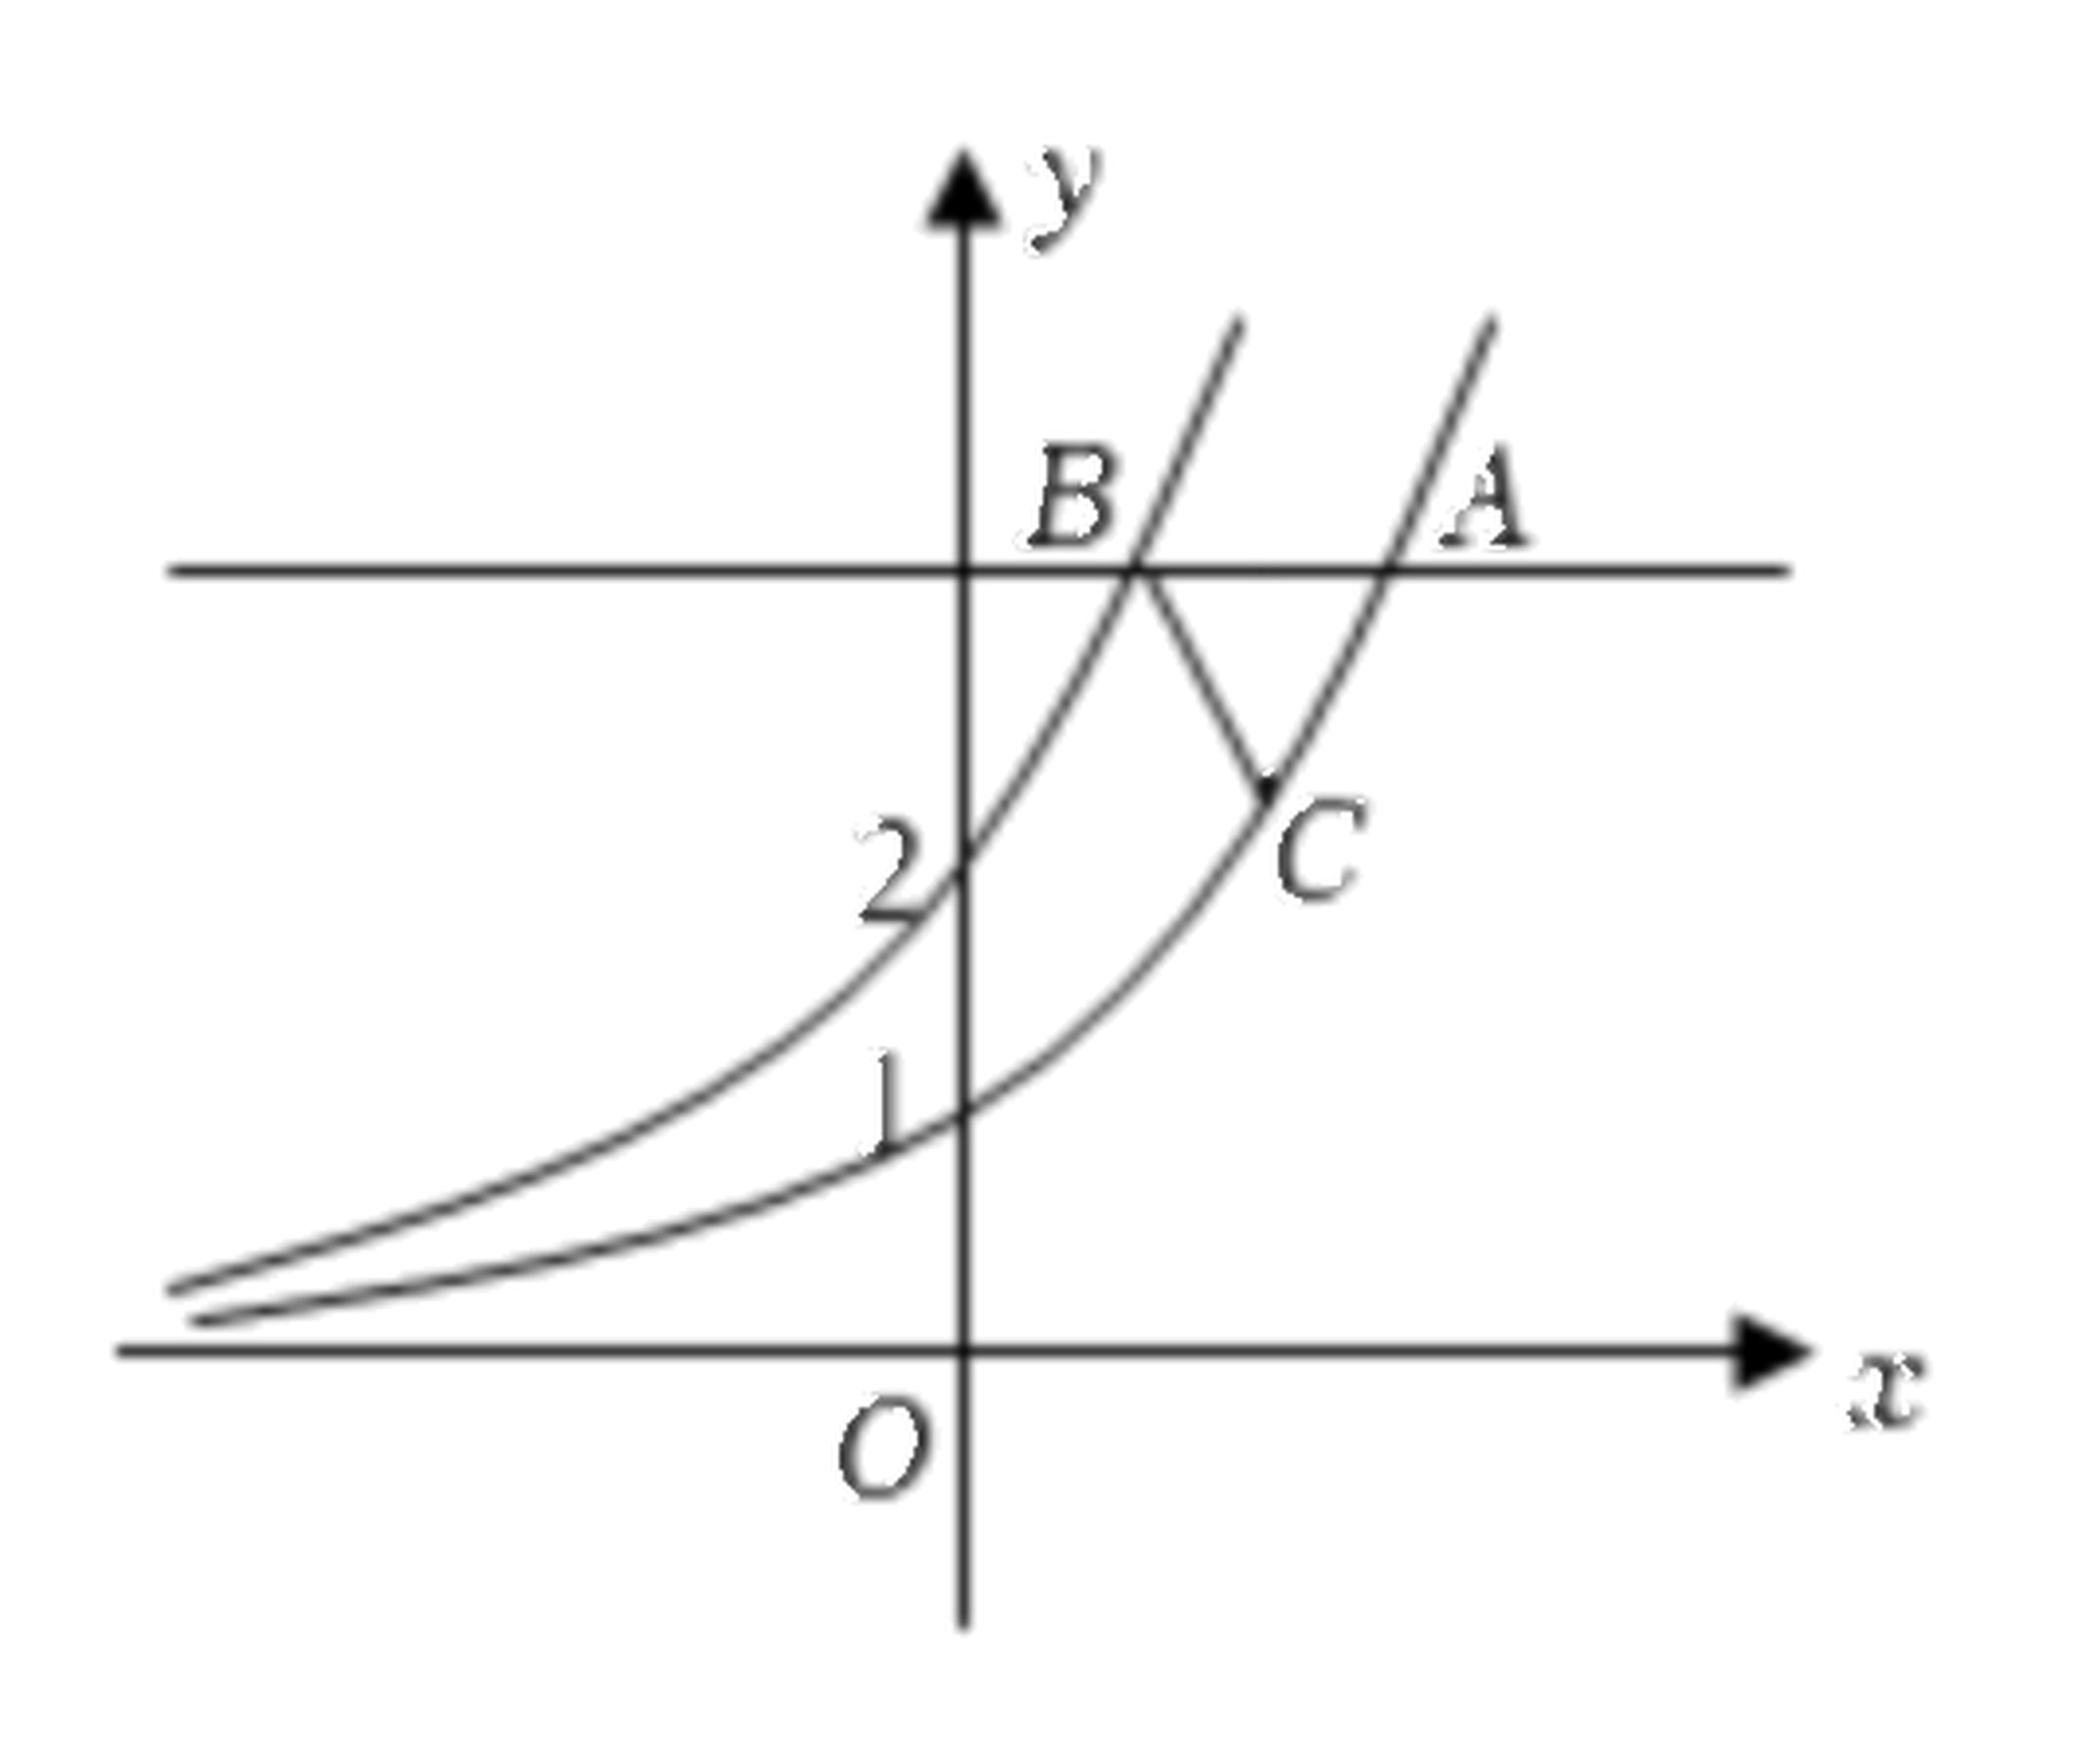
\includegraphics[width=0.40\textwidth]{figures/gao150_q11.png}
\end{center}

\ifanswer
\solbegin
\step{设直线 $l$ 的方程为 $y=a(a>0)$，}
\step{由 $2^x=a$，得 $x=\log_2 a$，所以 $A(\log_2 a,a)$，}
\step{由 $2^{x+1}=a$，得 $x=\log_2 a-1$，所以 $B(\log_2 a-1,a)$，所以 $\lvert AB\rvert=1$，}
\step{取 $AB$ 的中点 $D$，连接 $CD$，如图所示，}
\step{因为 $\triangle ABC$ 为等边三角形，则 $CD\perp AB$，且 $\lvert CD\rvert=\dfrac{\sqrt3}{2}$，}
\step{所以 $C\left(\log_2 a-\dfrac{1}{2},a-\dfrac{\sqrt3}{2}\right)$，}
\step{因为点 $C$ 在函数 $y=2^x$ 的图像上，所以 $a-\dfrac{\sqrt3}{2}=2^{\log_2 a-\frac{1}{2}}=\dfrac{a}{\sqrt2}$，}
\step{解得 $a=\dfrac{\sqrt3}{2-\sqrt2}=\dfrac{\sqrt3(2+\sqrt2)}{4-2}=\sqrt3+\dfrac{\sqrt6}{2}$，}
\step{所以点 $C$ 的纵坐标为 $a-\dfrac{\sqrt3}{2}=\dfrac{\sqrt3+\sqrt6}{2}$.}
\solend
\fi

% === Q12 === 解析配图（高斯函数方格阴影，仅答案版出）；"数学王子"弯引号；cases 块整体算一个印刷行；解析 4 行
\item 小玲在研究数学发展史，特别崇拜近代数学奠基者之一、享有“数学王子”称号的德国数学家高斯. 为了纪念高斯，我们把取整函数 $y=[x]$ 称为高斯函数，其中 $[x]$ 表示不超过 $x$ 的最大整数，如 $[1.1]=1$，$[-1.1]=-2$，则点集 $P=\{(x,y)\mid [x]^2+[y]^2=1\}$ 所表示的平面区域的面积为\blankline[4.4em].

\ifanswer
\solbegin
\step{$[x]^2+[y]^2=1$ 由 $\begin{cases}[x]=0\\ {[y]=-1}\end{cases}$ 或 $\begin{cases}[x]=0\\ {[y]=1}\end{cases}$ 或 $\begin{cases}[x]=-1\\ {[y]=0}\end{cases}$ 或 $\begin{cases}[x]=1\\ {[y]=0}\end{cases}$ 四个平面区域组成，}
\step{即 $\begin{cases}0\leqslant x<1\\ -1\leqslant y<0\end{cases}$ 或 $\begin{cases}0\leqslant x<1\\ 1\leqslant y<2\end{cases}$ 或 $\begin{cases}-1\leqslant x<0\\ 0\leqslant y<1\end{cases}$ 或 $\begin{cases}1\leqslant x<2\\ 0\leqslant y<1\end{cases}$，}
\step{作出平面区域如图所示，平面区域由四个边长为 $1$ 的正方形组成，}
\begin{center}
% 高斯函数 [x]^2+[y]^2=1 方格阴影区域图取 04 页顶部，去粉色水印、去色、4× LANCZOS 放大；仅答案版出
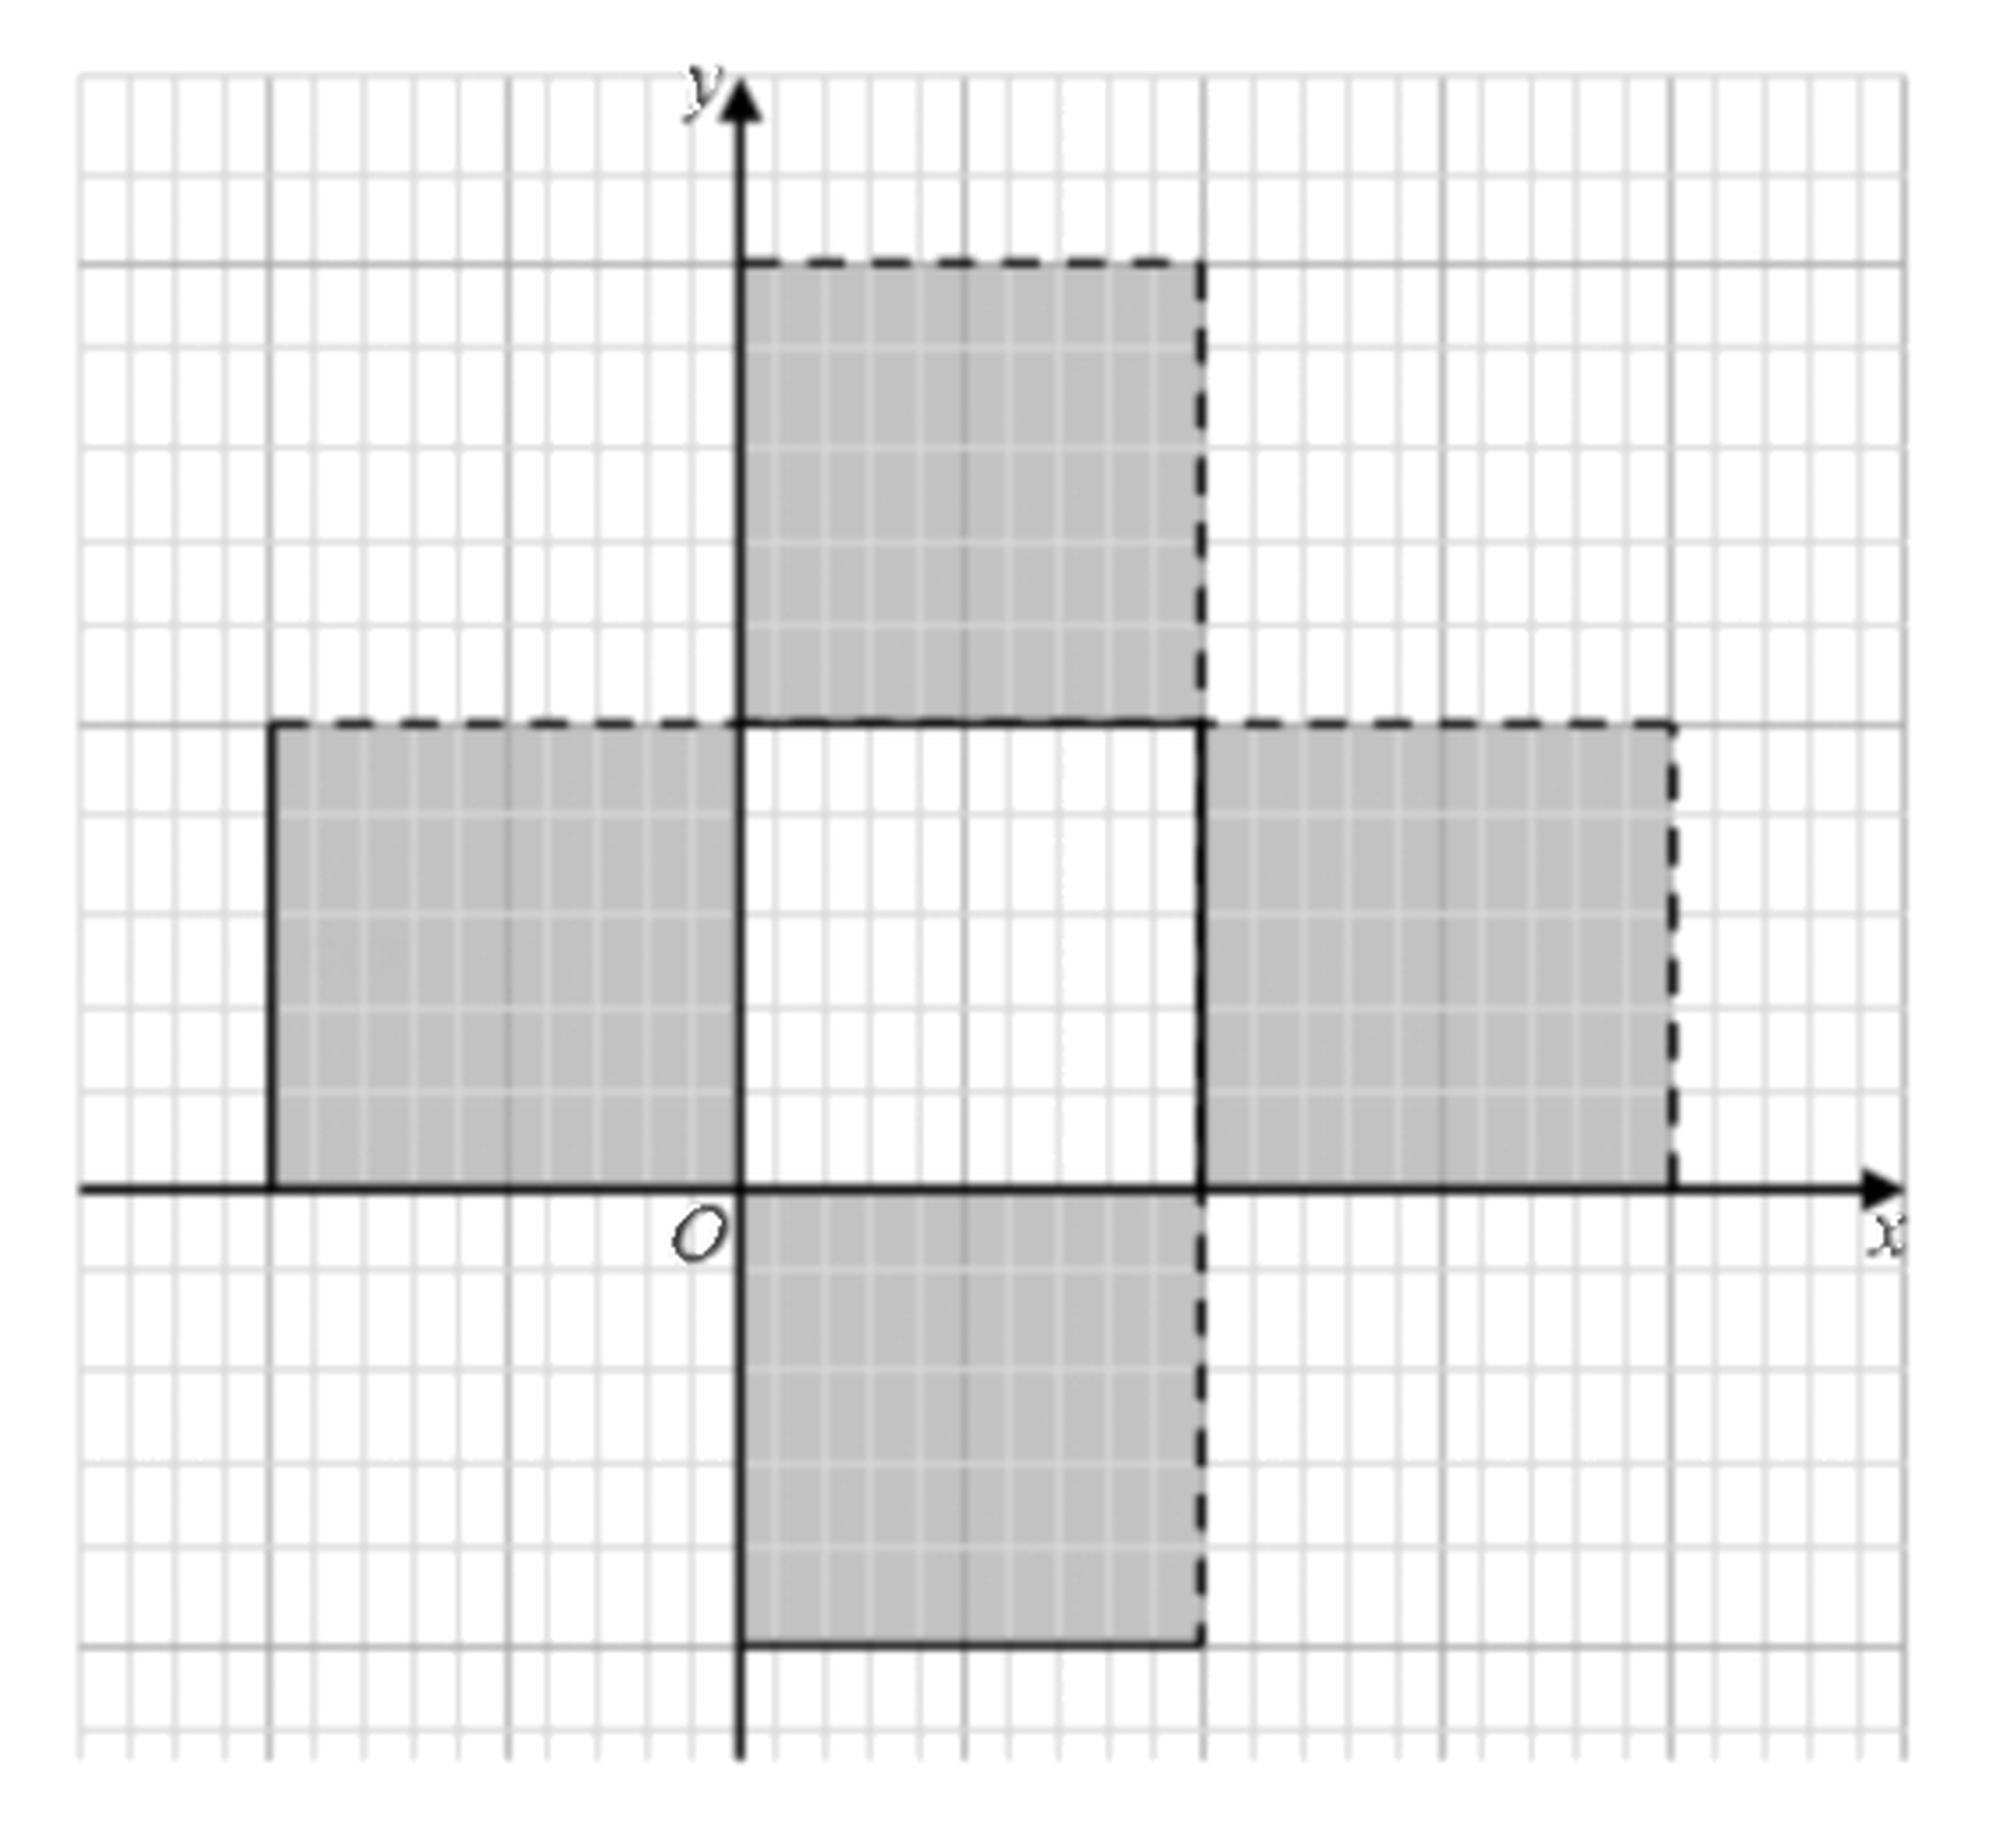
\includegraphics[width=0.34\textwidth]{figures/gao150_q12.png}
\end{center}
\step{总面积为 $1\times4=4$.}
\solend
\fi

\end{enumerate}

\bigsec{二、选择题}

\begin{enumerate}
\setcounter{enumi}{12}

% === Q13 === 答案在解析末句"故选 C"；括号 \mbox{（\quad）} 留空；四选项一行；解析 1 行
\item 设 $x\ne0$，则 $3^{\log_9 x^2}$ 的化简结果是\mbox{（\quad）}

\keepwithprev
A. $x$\qquad B. $\dfrac{1}{x}$\qquad C. $\lvert x\rvert$\qquad D. $\dfrac{1}{\lvert x\rvert}$

\ifanswer
\solbegin
\step{$3^{\log_9 x^2}=3^{\log_3\lvert x\rvert}=\lvert x\rvert$，故选 $C$.}
\solend
\fi

% === Q14 === 题目配图（两函数图像，三版都出）；\needvspace{8cm} 守卫放 \item 之前；"图像"照录；四选项两行两列；解析 2 行，故选 B
\needvspace{8cm}
\item 设 $a>0$ 且 $a\ne1$，$b\in\R$. 若函数 $y=a^{-\lvert x\rvert}$ 与 $y=x^b$ 的大致图像如图所示，则\mbox{（\quad）}

\keepwithprev
A. $0<a<1<b$\qquad\qquad B. $a>1$ 且 $b>1$

C. $0<a<1$ 且 $0<b<1$\qquad\qquad D. $0<b<1<a$

\begin{center}
% 两函数 y=a^{-|x|} 与 y=x^b 大致图像取 04 页右侧，去粉色水印、去色、4× LANCZOS 放大；三版都出
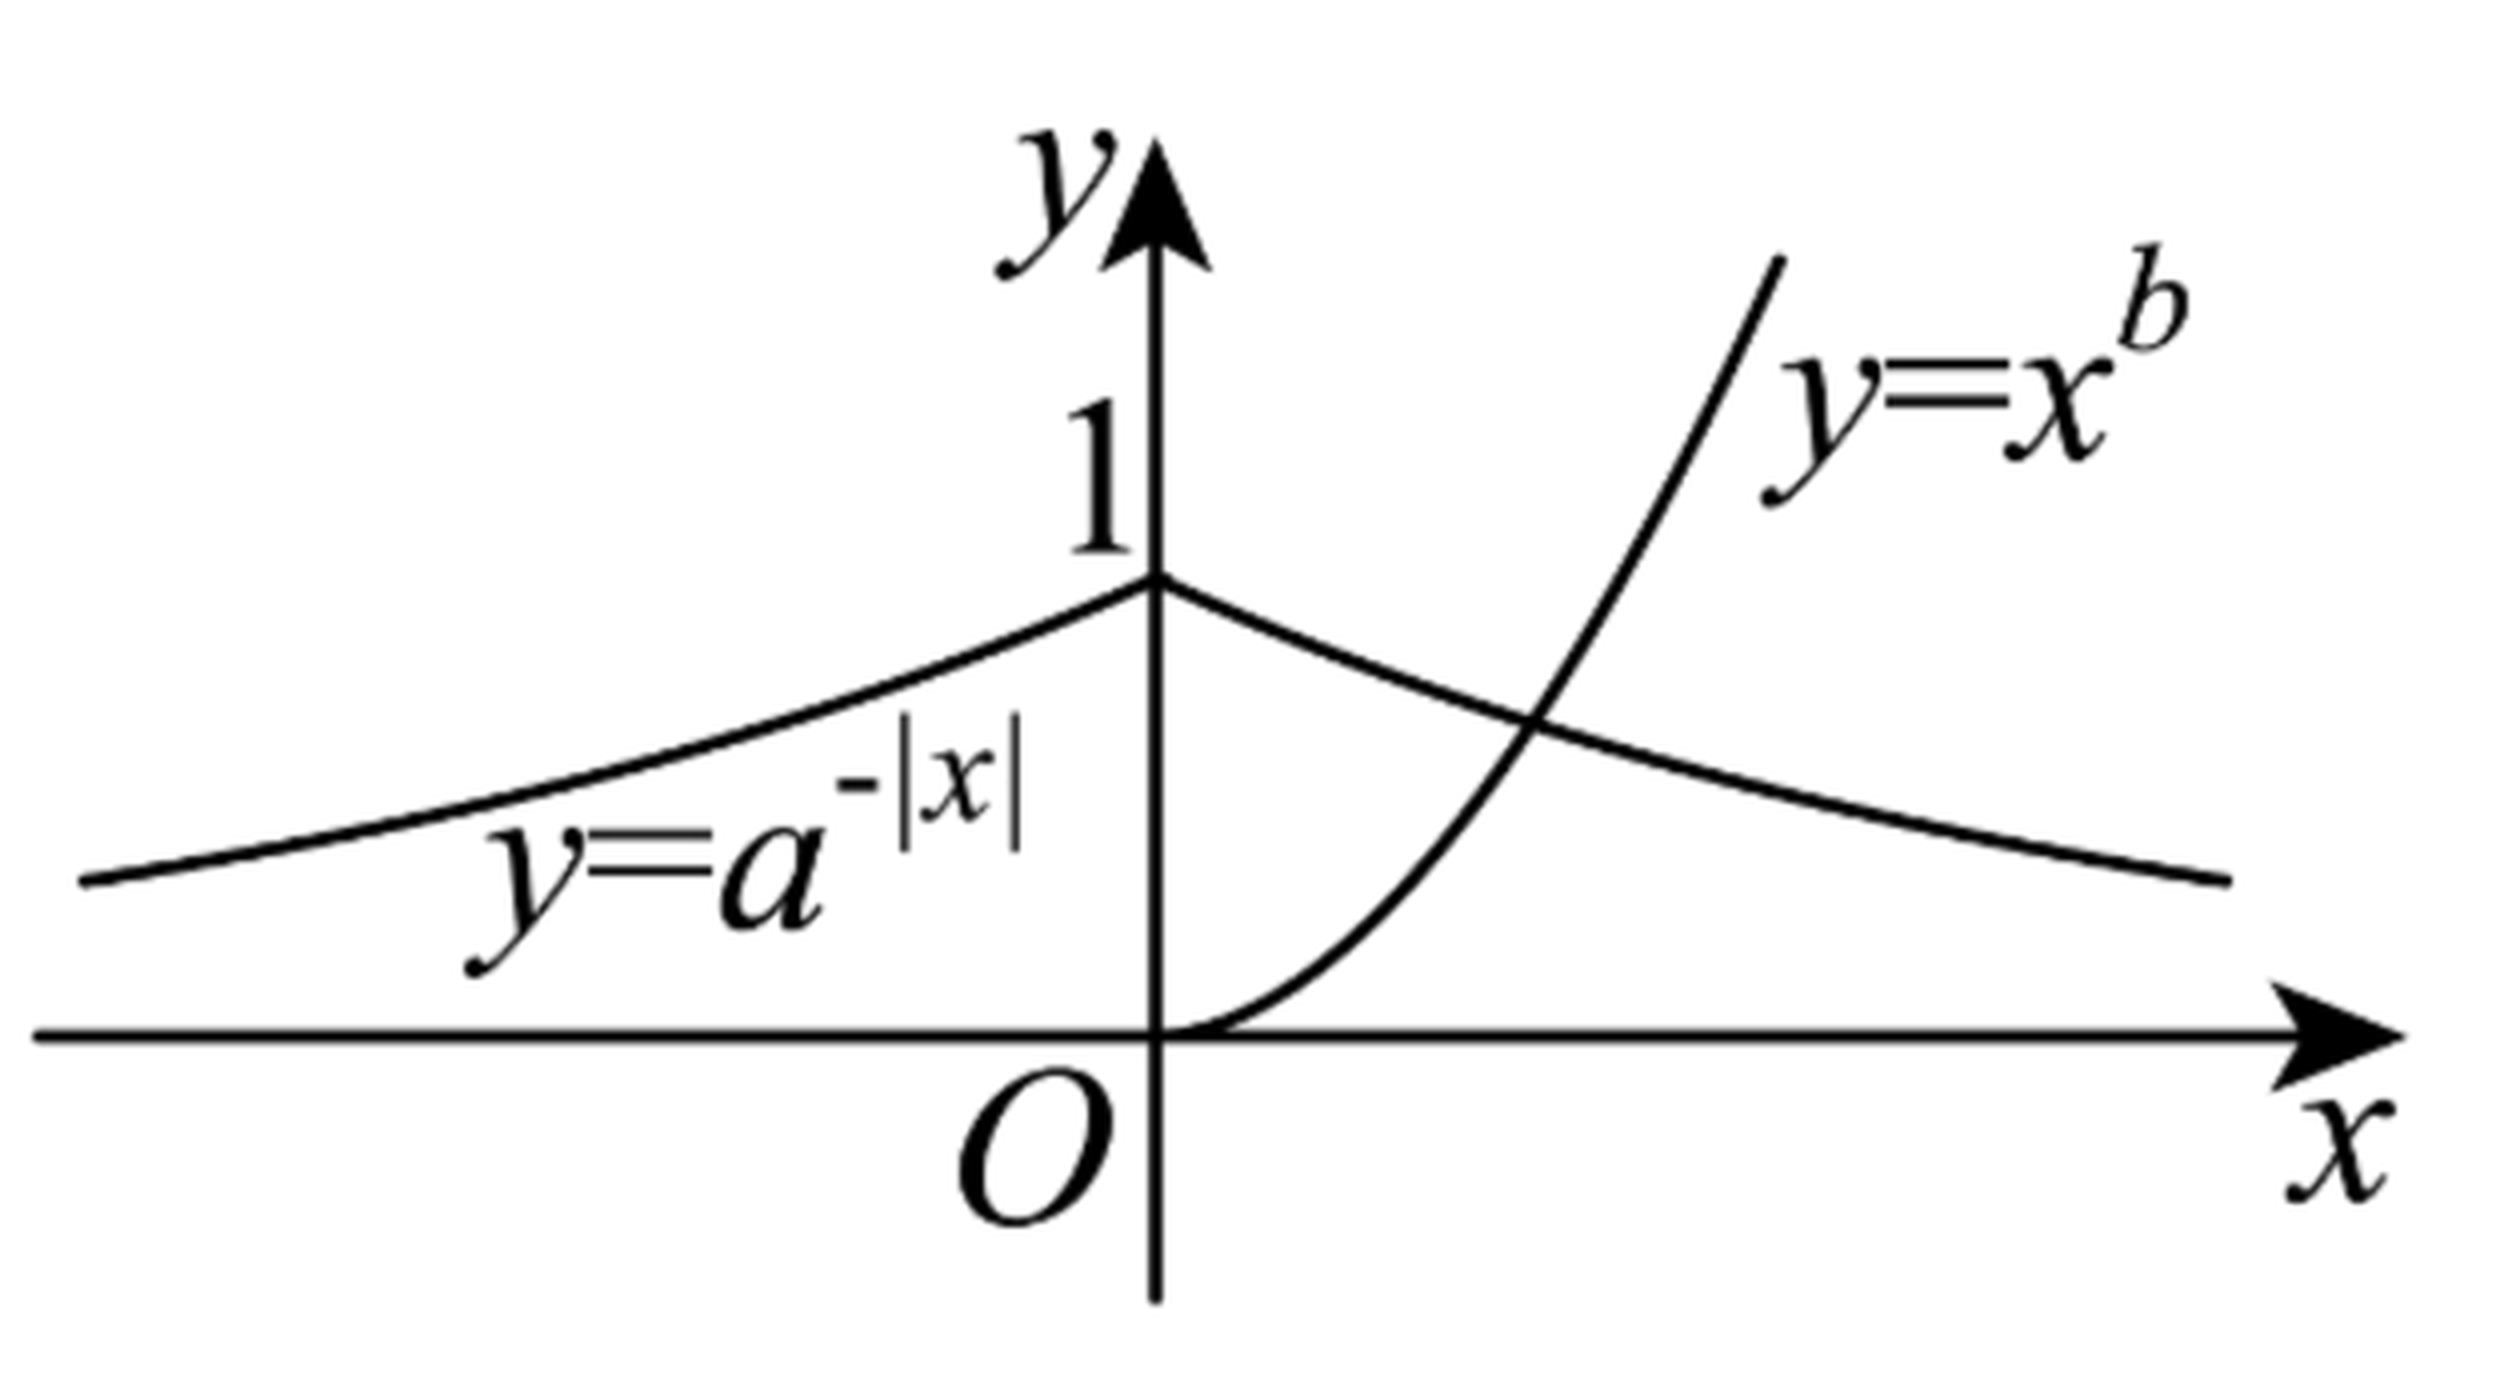
\includegraphics[width=0.40\textwidth]{figures/gao150_q14.png}
\end{center}

\ifanswer
\solbegin
\step{在 $(0,+\infty)$ 上，$y=a^{-x}$ 严格递减，得 $a>1$；}
\step{幂函数 $y=x^b$ 的图像递增且向上弯曲，得 $b>1$；故选 $B$.}
\solend
\fi

% === Q15 === "算术平均值／算术平均数"两处不同照录；四选项两行两列；解析 5 行（续 05 页顶），故选 B
\item 已知两个正数的算术平均值不小于它们的几何平均值，类比有以下结论：三个正数的算术平均数不小于它们的几何平均数，即当 $a,b,c$ 为正实数时，$\dfrac{a+b+c}{3}\geqslant\sqrt[3]{abc}$，当且仅当 $a=b=c$ 时等号成立. 利用上述结论，下列选项中判断正确的是\mbox{（\quad）}

\keepwithprev
A. 若 $x>0$，则 $2x+\dfrac{1}{x^2}\geqslant\dfrac{27}{8}$\qquad\qquad B. 若 $x>0$，则 $x^2+\dfrac{2}{x}\geqslant3$

C. 若 $0<x<1$，则 $x^2(1-x)\geqslant\dfrac{1}{9}$\qquad\qquad D. 若 $0<x<1$，则 $x^2(1-x)\leqslant\dfrac{1}{9}$

\ifanswer
\solbegin
\step{A：取 $x=1$，$2x+\dfrac{1}{x^2}=3<\dfrac{27}{8}$，错误.}
\step{B：$x^2+\dfrac{2}{x}=x^2+\dfrac{1}{x}+\dfrac{1}{x}\geqslant3\sqrt[3]{x^2\cdot\dfrac{1}{x}\cdot\dfrac{1}{x}}=3$，当且仅当 $x=1$ 时取等号，正确.}
\step{C：取 $x=\dfrac{1}{3}$，$x^2(1-x)=\dfrac{2}{27}<\dfrac{1}{9}$，错误.}
\step{D：取 $x=\dfrac{2}{3}$，$x^2(1-x)=\dfrac{4}{27}>\dfrac{1}{9}$，错误.}
\step{故选 $B$.}
\solend
\fi

% === Q16 === "完美集"新定义（弯引号、引号外空格照录）；圈数字①②文本模式；$n\in\N$；四选项两行两列；解析 9 行（6 行 05 页＋3 行 06 页顶），故选 A
\item 已知有限集 $A=\{a_1,a_2,\cdots,a_n\}$（$n\geqslant2$，$n\in\N$）. 若 $A$ 中元素 $a_i$（$i=1,2,\cdots,n$）满足 $a_1+a_2+\cdots+a_n=a_1\cdot a_2\cdots a_n$，就称 $A$ 为 “完美集”. 现有以下两个命题：

①恰有两个元素的 “完美集” 有无穷多个；

②若 $a_i$ 均为正整数，则 “完美集” $A$ 有且只有一个，且 $n=3$.

则\mbox{（\quad）}

\keepwithprev
A. ①和②都是真命题\qquad\qquad B. ①和②都是假命题

C. ①是真命题，②是假命题\qquad\qquad D. ①是假命题，②是真命题

\ifanswer
\solbegin
\step{①由 $a+b=ab\Leftrightarrow(a-1)(b-1)=1$，任取 $a>2$，则 $b=1+\dfrac{1}{a-1}\in(1,2)$，}
\step{得到无穷多个不同的完美集，①真.}
\step{②设 $1\leqslant a_1<a_2<\cdots<a_n$，则 $a_i\geqslant i$.}
\step{若 $n=2$，则 $(a_1-1)(a_2-1)=1$，只能有 $a_1=a_2=2$，与元素互异矛盾.}
\step{若 $n\geqslant4$，则 $a_1a_2\cdots a_n\geqslant a_2a_{n-1}a_n\geqslant2(n-1)a_n>na_n\geqslant a_1+\cdots+a_n$，矛盾.}
\step{当 $n=3$ 时，若 $a_1\geqslant2$，则 $a_1a_2a_3\geqslant6a_3>3a_3\geqslant a_1+a_2+a_3$，矛盾.}
\step{因此 $a_1=1$，$(a_2-1)(a_3-1)=2$，结合 $a_2<a_3$ 得 $a_2=2$，$a_3=3$.}
\step{唯一的完美集为 $\{1,2,3\}$，②真.}
\step{故选 $A$.}
\solend
\fi

\end{enumerate}

\bigsec{三、解答题}

\begin{enumerate}
\setcounter{enumi}{16}

% === Q17 === \varnothing 空集、$B\subseteq A$ 带下划线照录；弯引号内空格照录；解析 7 行
\item 设 $a,b\in\R$. 已知集合 $A=\{x\mid ax^2+3x-a>3\}$，$B=\{x\mid bx=1\}$.

(1) 若 $A=(1,2)$，求 $a$ 的值；

(2) 若 $a=0$，且 “ $x\in A$ ” 是 “ $x\in B$ ” 的必要非充分条件，求 $b$ 的取值范围.

\ifanswer
\solbegin
\step{(1) $A=(1,2)$，则 $a<0$，且 $1,2$ 是方程 $ax^2+3x-a-3=0$ 的两根.}
\step{由 $4a+6-a-3=0$，得 $a=-1$，此时不等式为 $-(x-1)(x-2)>0$，}
\step{解集确为 $(1,2)$.}
\step{(2) $a=0$ 时，$A=(1,+\infty)$，题意等价于 $B\subseteq A$ 且 $B\ne A$.}
\step{当 $b=0$ 时，$B=\varnothing$，符合条件.}
\step{当 $b\ne0$ 时，$B=\left\{\dfrac{1}{b}\right\}$，条件等价于 $\dfrac{1}{b}>1$，解得 $0<b<1$.}
\step{因此 $b$ 的取值范围为 $[0,1)$.}
\solend
\fi

% === Q18 === $p\in\Z$；"图像"（像，有亻）照录；指数 $-2p^2+5p$；解析 8 行（(1) 首行 06 页末＋2 行 07 页顶、(2) 5 行 07 页）
\item 设 $p\in\Z$，已知 $f(x)=x^{-2p^2+5p}$.

(1) 若幂函数 $y=f(x)$ 的图像关于原点成中心对称，且满足 $f(3)<f(4)$，求 $p$ 的值；

(2) 当 $p=-2$ 时，求满足 $f(2x+3)<f(x-4)$ 的 $x$ 的取值范围.

\ifanswer
\solbegin
\step{(1) 图像关于原点成中心对称，得整数 $-2p^2+5p$ 为奇数.}
\step{由 $f(3)<f(4)$，得 $-2p^2+5p>0\Leftrightarrow0<p<\dfrac{5}{2}$，}
\step{结合 $p\in\Z$，得 $p=1$ 或 $p=2$，对应指数分别为 $3$、$2$，所以 $p=1$.}
\step{(2) 当 $p=-2$ 时，$f(x)=\dfrac{1}{x^{18}}$，定义域为 $\{x\in\R\mid x\ne0\}$.}
\step{原不等式要求 $x\ne-\dfrac{3}{2}$ 且 $x\ne4$，}
\step{此时 $\dfrac{1}{(2x+3)^{18}}<\dfrac{1}{(x-4)^{18}}\Leftrightarrow\lvert 2x+3\rvert>\lvert x-4\rvert\Leftrightarrow(2x+3)^2>(x-4)^2$，}
\step{因此 $(x+7)(3x-1)>0\Leftrightarrow x<-7$ 或 $x>\dfrac{1}{3}$，}
\step{排除 $x=4$，得 $x\in(-\infty,-7)\cup\left(\dfrac{1}{3},4\right)\cup(4,+\infty)$.}
\solend
\fi

% === Q19 === $a\in\R$、$g(x)=f(2x+1)+a\cdot f(x)+2$；解析 6 行（(2) 末两行续 08 页顶）
\item 已知 $f(x)=2^x$.

(1) 求方程 $f(2x)-f(x)=6$ 的解；

(2) 设 $a\in\R$，$g(x)=f(2x+1)+a\cdot f(x)+2$，若对于任意 $x\in[-1,1]$，均有 $g(x)\geqslant1$，求 $a$ 的取值范围.

\ifanswer
\solbegin
\step{(1) 令 $t=2^x>0$，则 $t^2-t-6=(t-3)(t+2)=0$，}
\step{由 $t>0$ 得 $t=3$，所以 $x=\log_2 3$.}
\step{(2) 令 $t=2^x$，则 $t\in\left[\dfrac{1}{2},2\right]$，且 $g(x)\geqslant1\Leftrightarrow2t^2+at+1\geqslant0\Leftrightarrow a\geqslant-\left(2t+\dfrac{1}{t}\right)$，}
\step{由基本不等式得 $2t+\dfrac{1}{t}\geqslant2\sqrt{2t\cdot\dfrac{1}{t}}=2\sqrt2$，}
\step{当且仅当 $t=\dfrac{1}{\sqrt2}\in\left[\dfrac{1}{2},2\right]$ 时等号成立，}
\step{因此 $-\left(2t+\dfrac{1}{t}\right)$ 的最大值为 $-2\sqrt2$，所求范围为 $a\in[-2\sqrt2,+\infty)$.}
\solend
\fi

% === Q20 === "极闭集"新定义、3 问，全卷末题；$M\subseteq(0,+\infty)$ 带下划线照录；自定义运算 $x*y$ 星号照录；解析 13 行（9 行 08 页＋4 行 09 页上半）
\item 对于非空实数集 $M\subseteq(0,+\infty)$，若满足以下两个条件：

① $M$ 中至少含有 $2$ 个元素，且 $1\notin M$；

②对于 $M$ 中任意两个不相等的元素 $x$、$y$，定义 $x*y=\dfrac{xy+1}{x+y}$，且 $x*y\in M$.

则称 $M$ 为 “极闭集”.

(1) 分别判断集合 $A=\left\{\dfrac{1}{2},3\right\}$ 与集合 $B=(1,+\infty)$ 是否为 “极闭集” （无需理由）；

(2) 若 $M$ 是 “极闭集”，证明：$M$ 中不可能所有元素都小于 $1$；

(3) 证明：不存在任何有限集是 “极闭集”.

\ifanswer
\solbegin
\step{(1) $A$ 不是 “极闭集”，$B$ 是 “极闭集”.}
\step{(2) 假设 $M$ 中所有元素都小于 $1$，取其中两个不相等的元素 $x$、$y$，}
\step{则 $x*y-1=\dfrac{(1-x)(1-y)}{x+y}>0$，}
\step{这与 $x*y\in M$ 且 $M$ 中所有元素都小于 $1$ 矛盾.}
\step{(3) 假设有限集 $M$ 是 “极闭集”，}
\step{由 (2) 及 $1\notin M$，得 $M$ 中存在大于 $1$ 的元素.}
\step{若 $M$ 中有小于 $1$ 的元素，取其中最大的一个为 $a$，另取 $b\in M$ 且 $b>1$，}
\step{则 $a*b-a=\dfrac{1-a^2}{a+b}>0, a*b-1=\dfrac{(a-1)(b-1)}{a+b}<0$，}% 半角逗号在两个数学式组之间，全稿惯例、非笔误，照录
\step{于是 $a<a*b<1$ 且 $a*b\in M$，与 $a$ 的最大性矛盾.}
\step{若 $M$ 中没有小于 $1$ 的元素，则 $M\subseteq(1,+\infty)$.}
\step{取 $a=\min M$，另取 $b\in M$ 且 $b\ne a$，则 $a*b-a=\dfrac{1-a^2}{a+b}<0$，}
\step{于是 $a*b<a$ 且 $a*b\in M$，与 $a$ 的最小性矛盾.}
\step{因此不存在任何有限集是 “极闭集”.}
\solend
\fi

\end{enumerate}

\end{document}
"
%
% ① 原始材料：微信公众号"魔都数学加油站"文章，连载"27学年高一150"，原文标题
% "27学年高一150——2026-2027年上海市曹杨二中高一上期中"；
% 原文链接：https://mp.weixin.qq.com/s/xlQxmik8TZXR87RC6MnCrw 。
% 正文为 9 张 PNG 页（01/02/04/06/07/09 为 2560×3620，03/05/08 为 4762×6735，
% 同一篇各页分辨率混排，逐页按各自分辨率裁图核对，别按预览比例换算裁框）。
% 体例：讲评版——全 18 题均印【解析】（逐题核实，见 ② ②）。
% 题目、答案、解析均据原图转录；卷面粉红色/红色水印"魔都数学加油站"及公众号页脚未录入。
% 全卷插图清单（逐页通读 9 页确认）：3 幅——
%   · Q11 题目配图（指数函数曲线图，02 页右侧：x/y 轴、O、y=2^x 与 y=2^{x+1}
%     两曲线、A/B/C 三点、刻度 1/2、等边三角形 ABC），三版都出，裁 figures/gao150_q11.png；
%   · Q12 解析配图（高斯函数取整 [x]^2+[y]^2=1 方格阴影区域图，04 页顶部：4 个边长 1
%     的正方形组成的十字形阴影），解析"作出平面区域如图所示"处，仅答案版出，
%     放 \ifanswer 内 \step 之间，裁 figures/gao150_q12.png；
%   · Q14 题目配图（两函数 y=a^{-|x|} 与 y=x^b 大致图像，04 页右侧：x/y 轴、O、
%     y 轴刻度 1、一递减曲线一递增上翘曲线），三版都出，裁 figures/gao150_q14.png；
%   其余各页逐页确认无其它题目配图、无表格；Q11/Q12 解析"如图所示"对应的就是上列
%   已裁的图，不重复裁；09 页上半为 Q20(3) 解析续尾、下半仅水印、无正文。
%   3 图均取自原卷截图，去粉色水印、去色、4× LANCZOS 放大。
%
% 卷首标题：原卷印作"2026-2027 年曹杨二中高一上期中"，年份区间按全稿惯例排 en dash；
% 原卷卷面未印副标题，本稿按同期中卷知识模块口径补出"集合与常用逻辑用语、不等式、函数"。
%
% 题号体例（逐页核实定稿）：本卷共 18 题——一、填空题 3—12（10 题）、
% 二、选择题 13—16（4 题）、三、解答题 17—20（4 题）。
% 三节分别 \setcounter{enumi}{2}／{12}／{16}。原卷从第 3 题起、无第 1、2 题，
% 本稿保留原题号；全卷末题为第 20 题（"极闭集"新定义、3 问），无 Q21、无附加题节。
%
% ② 与原卷的排版差异：
%   ① 原文从第 3 题起，本稿保留原题号；共 18 题三节，解答题只有 4 题到 20；
%   ② 全 18 题均印【解析】，用 \solbegin…\solend；逐题核实无只印【答案】或
%      答案印题干括号内的题；四道选择题答案在解析末句"故选 X"（Q13 选 C、
%      Q14 选 B、Q15 选 B、Q16 选 A，逐个放大复核）、括号 \mbox{（\quad）} 留空、
%      不另提 \ans{}；答案版【答案】/【解析】标记数 = 18 = 全卷题数；
%   ③ 原卷卷面未印副标题，本稿按知识模块口径补出；
%   ④ 原卷填空横线按全稿惯例排 \blankline[4.4em]；选择题括号排 \mbox{（\quad）}、
%      选项段前按惯例加 \keepwithprev；解答题不留作答区、不加 \anspace（原卷为讲评版）；
%   ⑤ 数集黑板粗体：Q4"m\in R"、Q5"a,b\in R"、Q6"a,b,c\in R"、Q7"a\in R"、
%      Q10"a\in R"、Q14"b\in R"、Q17"a,b\in R"、Q18"p\in Z"／定义域"x\in R"、
%      Q19"a\in R"、Q16"n\in N" 原卷印斜体 R/Z/N，按全稿惯例归一 \R／\Z／\N；
%      绝对值排 \lvert…\rvert（Q7 |x+4|+|x-3|、Q11 |AB|／|CD|、Q13 |x|、
%      Q18 |2x+3|／|x-4|），集合描述竖线排 \mid（Q3、Q12、Q17、Q18、Q20），
%      不等号按全稿惯例排 \leqslant／\geqslant；补集照原卷上划线排 \overline{A}
%      （Q3 题干＋解析共 2 处）；空集符号 \varnothing（Q17 解析(2)）；
%      子集 \subset（单线⊂）／\subseteq（带下划线⊆）逐处照录，本卷 3 处子集
%      符号均印带下划线 ⊆、照录 \subseteq（Q20 题干、Q20 解析(3)、Q17 解析(2)，
%      见 ④），无 \subset 用例；
%   ⑥ 判别式 Δ/△：逐页通读 9 页，本卷无一元二次判别式算式，故无 Δ/△ 混用可照录
%      （"高 \Delta／扁 \triangle"口径备查，参照 高一142／144／145／146／148／149
%      头注④）；本卷仅 Q11 题干与解析共 2 处几何三角形符号 △ABC，逐处放大并排
%      确认两处同形、印近等边粗线三角（非判别式），照录 \triangle（见 ④）；
%   ⑦ 中文弯引号照录：Q12"数学王子"、Q16"完美集"（题干＋①②两命题，引号外
%      留空格）、Q17" x∈A "" x∈B "（引号内空格）、Q20"极闭集"（题干条件、
%      三问与解析，引号外留空格）；注释里一律 ASCII 引号；数学式内 CJK 用 \text{}
%      （Q3 集合描述"且"用 \text{ 且 }）；
%   ⑧ 半角逗号在数学组之间是全稿惯例、非笔误，逐处照录（Q17 解析"1,2 是方程…
%      两根"、Q20 解析(3)">0, a*b-1=…<0" 两式之间等）；行末西文句点 ASCII `.`；
%      行中全角逗号／顿号照录（Q12"之一、享有"、Q18 解析"3、2"、Q20"x、y"）；
%   ⑨ "图像／图象"逐处放大核：全卷 9 处均印"图像"（像，有亻）、未见"图象"——
%      Q4 题干 1、Q11 题干 2＋解析 1、Q14 题干 1＋解析 1、Q18 题干 1＋解析 1；
%      同卷"第二象限""象限"用"象"（无亻）。逐处照录未统一改动（放大 01/02/04/06
%      页 /tmp/gao150/z/p01_q4_tuxiang2.png、p04_q14_tuxiang2.png、
%      p02_q11_lines.png 确认）；子题标号 (1)(2)(3) 半角括号照录；圈数字①②
%      在文本模式（Q16 两命题与解析、Q20 两条件与三问及解析）按 common.sty
%      划入 CJK 字符类渲染，进数学式用 \text{①}；
%   ⑩ Q20 新定义 x*y=\dfrac{xy+1}{x+y} 的 * 是自定义运算（星号），照录；
%      \left…\right 不得拆到不同 $…$ 组（Q19"\left(2t+\frac1t\right)"、
%      Q20 题干"A=\left\{\frac12,3\right\}"等）；Q8 嵌套根号
%      \sqrt{\frac2x+\frac{16}{1-2x}}、Q9 对数连加 \log_2 A 等复杂式照录别简化；
%   ⑪ 一条 \step = 原卷解析的一个印刷行，cases 块整体算一个印刷行；别并折行、
%      别拆行。Q4 三行、Q8 五行、Q11 九行、Q12 四行（两行各含四个 cases 块）、
%      Q15 五行、Q16 九行、Q18 八行、Q20 十三行均按印刷行逐条断，不丢行；
%   ⑫ 配图：Q11／Q14 题目配图（三版都出）放 \item 内题干之后 \begin{center}，
%      大图块加 \needvspace{8cm} 守卫把整块推走（守卫放 \item 之前，见
%      高一145 Q14/Q20 成例与切页审计 B 类坑）；Q12 解析配图（仅答案版出）
%      放 \ifanswer 内 \solbegin…\solend 的 \step 之间（高一73 第16题成例）；
%   ⑬ 跨页续印按题合并：见 ⑥；
%   ⑭ 原卷解析内无红色"法一／法二"之类小标题，故本卷无 \stepm；红色水印
%      "魔都数学加油站"不录入；Q12 解析"作出平面区域如图所示"对应的图即
%      ① 所列 gao150_q12.png（04 页顶部），不重复裁；Q11 解析"如图所示"对应
%      题目配图 gao150_q11.png，不另裁。
%
% ③ 行数复核：一条 \step／\stepm = 原卷解析的一个印刷行，cases 块作一个印刷行计。
%   逐题数（主会话逐页核对定稿）：Q3：1；Q4：3；Q5：2；Q6：1；Q7：2；Q8：5；
%   Q9：1；Q10：3；Q11：9；Q12：4；Q13：1；Q14：2；Q15：5；Q16：9；
%   Q17：7；Q18：8；Q19：6；Q20：13。
%   合计 82 条 \step（本卷无 \stepm：解析内无红色"法一／法二"类小标题），
%   与原卷逐题印刷行相等。全卷 18 题均设 \solbegin…\solend，答案版
%   【答案】/【解析】标记数 = 18 = 全卷题数。
%
% ④ 判别式／三角形／子集符号结论（逐处放大原图照录、不得统一，主会话像素级复核）：
%   判别式：逐页通读 9 页，本卷无一元二次判别式 Δ/△ 算式（Q18 讨论幂函数指数
%     奇偶、不用判别式；Q9／Q19／Q20 亦无），头注 ② ⑥ 的"高 \Delta／扁 \triangle"
%     口径在本卷无对应处（参照 高一142／144／145／146／148／149 头注④，仅备查）。
%   几何三角形符号：Q11 题干"使得 △ABC 为等边三角形"（02 页末）与解析
%     "因为 △ABC 为等边三角形，则 CD⊥AB"（03 页）共 2 处，放大 02/03 页
%     /tmp/gao150/z/q11_tri_montage2.png 并排确认两处同形、印近等边粗线三角
%     （h/w≈0.98、非"高>宽"的判别式 \Delta），照录 \triangle（与 高一105
%     "使得 \triangle ABC 为等边三角形" 同短语成例、高一149 几何三角形照录
%     \triangle 口径一致），不引入 \Delta。
%   子集／补集：Q20 题干"$M\subseteq(0,+\infty)$"（08 页）、Q20 解析(3)
%     "则 $M\subseteq(1,+\infty)$"（09 页）、Q17 解析(2)"题意等价于 $B\subseteq A$
%     且 $B\ne A$"（06 页）共 3 处子集符号，逐处放大（/tmp/gao150/z/p08_q20_stem.png、
%     p09_q20_sub.png、p06_q17_sub.png）确认均印带下划线 ⊆，照录 \subseteq；
%     本卷未见单线 ⊂（\subset）之对应处。Q3 题干与解析共 2 处补集照原卷上划线
%     排 \overline{A}；Q17 解析(2) 空集印 ∅、照录 \varnothing（Q7"解集为空集"
%     为中文词、非符号，照录文字）；集合描述竖线 \mid；数集 \R／\Z／\N 归一见 ② ⑤。
%
% ⑤ 存疑照录（放大原图确认，照录未改、正文对应处另有 % 注）：
%   1. Q8 解析第 4 行"所以 $y=\frac1x+\frac{8}{1-2x}$ 的最小值为 18" —— 上文
%      并未定义 $y$，且题面求的是 $\sqrt{\frac2x+\frac{16}{1-2x}}$ 的最小值；
%      按上下文该行应为 $\frac1x+\frac{8}{1-2x}$ 的最小值为 18（$y$ 疑为原卷
%      衍字／笔误），放大 02 页 /tmp/gao150/z/p02_q8_y.png 确认，照录未改。
%   2. Q20 解析(3)"$a*b-a=\frac{1-a^2}{a+b}>0, a*b-1=\frac{(a-1)(b-1)}{a+b}<0$"
%      两式之间的逗号原卷印半角 ,（非全角），按全稿惯例"半角逗号在数学组之间"
%      照录未改（放大 08 页 /tmp/gao150/z/p08_q20_sol8.png 确认）。
%   3. Q15 题干"两个正数的算术平均值…几何平均值"与"三个正数的算术平均数…
%      几何平均数"两处"值／数"用字不同，逐处照录未统一（放大 04 页确认）。
%   4. "图像／图象"全卷 9 处均印"图像"（像，有亻）、未见"图象"，逐处放大核实
%      照录、未统一改动（见 ② ⑨）；本卷判别式 Δ/△ 无用例、几何三角形 2 处
%      照录 \triangle（见 ④）。
%   全卷除此 4 类外未发现其它笔误／自相矛盾处；18 题均印【解析】、无只印【答案】
%   或答案印题干括号内的题（见 ② ②）。
%
% ⑥ 跨页续印按题合并说明（逐页核实定稿）：Q3/4/5/6/7 题干＋解析在 01 页；
%   Q8 题干＋解析 5 行、Q9 题干＋解析 1 行在 02 页上半；Q10 题干＋解析 3 行
%   在 02 页下半；Q11 题干（前两行）＋配图在 02 页下半、题干续"三角形，则点 C
%   的纵坐标为___"与解析 9 行全在 03 页上半（解析"如图所示"对应题目配图）；
%   Q12 题干＋解析 4 行在 03 页下半，解析配图（方格阴影）续印在 04 页顶部；
%   "二、选择题"标题在 04 页中部；Q13 题干＋选项＋解析、Q14 题干＋选项＋
%   配图＋解析在 04 页；Q15 题干＋四选项在 04 页末、解析 5 行续 05 页上半；
%   Q16 题干＋①②两命题＋"则(  )"＋四选项＋解析前 6 行在 05 页、解析末 3 行
%   （"因此 a_1=1…②真""故选 A"）续 06 页顶部；"三、解答题"标题在 06 页；
%   Q17 题干(1)(2)＋解析(1) 3 行＋解析(2) 首行在 06 页、解析(2) 续 3 行
%   在 06 页下半；Q18 题干(1)(2)＋解析(1) 首行在 06 页末、解析(1) 续 2 行＋
%   解析(2) 5 行在 07 页上半；Q19 题干(1)(2)＋解析(1) 2 行＋解析(2) 前 2 行
%   在 07 页下半、解析(2) 末 2 行续 08 页顶部；Q20 题干（新定义＋①②两条件）
%   ＋三问＋解析(1)(2)(3) 前 9 行在 08 页、解析(3) 末 4 行续 09 页上半，
%   末行"因此不存在任何有限集是极闭集"为全卷收尾（09 页下半仅水印、无正文）。
%   本稿按题连排，不丢行、不并折行；全卷末题为第 20 题，无 Q21、无附加题节。
%
\documentclass[a4paper,11pt]{article}
\usepackage{common}

\begin{document}

\examtitlest[3]{2026--2027 年曹杨二中高一上期中}{集合与常用逻辑用语、不等式、函数}

\bigsec{一、填空题}

\begin{enumerate}
\setcounter{enumi}{2}

% === Q3 === 补集上划线 \overline{A}（题干＋解析各 1 处）；集合描述竖线 \mid、数学式内"且"用 \text{}；解析 1 行
\item 设全集 $U=\{1,2,3,4,5\}$，集合 $A=\{x\mid x^2-3x\leqslant0\text{ 且 }x\in U\}$，则 $\overline{A}=$\blankline[4.4em].

\ifanswer
\solbegin
\step{$x^2-3x\leqslant0\Leftrightarrow0\leqslant x\leqslant3$，所以 $A=\{1,2,3\}$，$\overline{A}=\{4,5\}$.}
\solend
\fi

% === Q4 === "图像"（像，有亻）逐处照录、同句"第二象限"用"象"（无亻）；解析 3 行
\item 设 $m\in\R$. 若幂函数 $y=(m^2-5m+1)x^{m+1}$ 的图像经过第二象限，则 $m=$\blankline[4.4em].

\ifanswer
\solbegin
\step{幂函数的系数为 1，故 $m^2-5m+1=1\Rightarrow m=0$ 或 $m=5$.}
\step{$m=0$ 时，$y=x$ 不经过第二象限；}
\step{$m=5$ 时，$y=x^6$ 经过第二象限，因此 $m=5$.}
\solend
\fi

% === Q5 === 解析 2 行
\item 设 $a,b\in\R$. 若 $a^2+\dfrac{b^2}{4}=1$，则 $ab$ 的最大值为\blankline[4.4em].

\ifanswer
\solbegin
\step{$1-ab=\left(a-\dfrac{b}{2}\right)^2\geqslant0$，即 $ab\leqslant1$；}
\step{当 $a=\dfrac{\sqrt2}{2}$，$b=\sqrt2$ 时取等号，最大值为 1.}
\solend
\fi

% === Q6 === 解析 1 行
\item 设 $a,b,c\in\R$. 若等式 $2x^2-3x-2=a(x-1)^2+b(x-1)+c$ 恒成立，则 $a-b+c=$\blankline[4.4em].

\ifanswer
\solbegin
\step{令 $x=0$，得 $a-b+c=-2$.}
\solend
\fi

% === Q7 === 绝对值 \lvert…\rvert；解析 2 行
\item 设 $a\in\R$. 若关于 $x$ 的不等式 $\lvert x+4\rvert+\lvert x-3\rvert<a$ 的解集为空集，则 $a$ 的取值范围是\blankline[4.4em].

\ifanswer
\solbegin
\step{$\lvert x+4\rvert+\lvert x-3\rvert\geqslant\lvert(x+4)-(x-3)\rvert=7$，当 $-4\leqslant x\leqslant3$ 时取等号.}
\step{原不等式的解集为空集当且仅当 $a\leqslant7$，即 $a\in(-\infty,7]$.}
\solend
\fi

% === Q8 === 嵌套根号 \sqrt{\frac{2}{x}+\frac{16}{1-2x}} 照录别简化；解析 5 行
\item 设 $x\in\left(0,\dfrac{1}{2}\right)$，则 $\sqrt{\dfrac{2}{x}+\dfrac{16}{1-2x}}$ 的最小值为\blankline[4.4em].

\ifanswer
\solbegin
\step{因为 $x\in\left(0,\dfrac{1}{2}\right)$，所以 $1-2x>0$，又 $2x+1-2x=1$，}
\step{所以 $\left(\dfrac{1}{x}+\dfrac{8}{1-2x}\right)(2x+1-2x)=10+\dfrac{1-2x}{x}+\dfrac{16x}{1-2x}$}
\step{$\geqslant10+2\sqrt{\dfrac{1-2x}{x}\cdot\dfrac{16x}{1-2x}}=18$，}
\step{当且仅当 $\dfrac{1-2x}{x}=\dfrac{16x}{1-2x}$ 即 $x=\dfrac{1}{6}$ 时取等号，所以 $y=\dfrac{1}{x}+\dfrac{8}{1-2x}$ 的最小值为 18，}% 原卷此处径写 $y=\frac1x+\frac{8}{1-2x}$（上文未定义 $y$、且与题面根式不符），疑笔误，放大 02 页确认，照录未改（见 ⑤）
\step{所以 $\sqrt{\dfrac{2}{x}+\dfrac{16}{1-2x}}$ 的最小值为 6.}
\solend
\fi

% === Q9 === 对数连加 \log_2 A 等复杂式照录别简化；解析 1 行
\item 记 $A=1\times2\times3\times\cdots\times2026$，则 $\dfrac{1}{\log_2 A}+\dfrac{1}{\log_3 A}+\dfrac{1}{\log_4 A}+\cdots+\dfrac{1}{\log_{2026}A}=$\blankline[4.4em].

\ifanswer
\solbegin
\step{原式 $=\log_A 2+\cdots+\log_A 2026=\log_A(2\times3\times\cdots\times2026)=\log_A A=1$.}
\solend
\fi

% === Q10 === "严格减函数／不恒为负／⇔"照录；解析 3 行
\item 设 $a\in\R$，$f(x)=\dfrac{ax+1}{x+2}$. 若函数 $y=f(x)$ 在 $[1,+\infty)$ 上是严格减函数，且在 $[1,+\infty)$ 上的函数值不恒为负，则 $a$ 的取值范围是\blankline[4.4em].

\ifanswer
\solbegin
\step{当 $1\leqslant x_1<x_2$ 时，$f(x_2)-f(x_1)=\dfrac{(2a-1)(x_2-x_1)}{(x_1+2)(x_2+2)}$，故严格递减 $\Leftrightarrow a<\dfrac{1}{2}$.}
\step{此时最大函数值为 $f(1)$，函数值不恒为负 $\Leftrightarrow f(1)=\dfrac{a+1}{3}\geqslant0\Leftrightarrow a\geqslant-1$，}
\step{得 $a\in\left[-1,\dfrac{1}{2}\right)$.}
\solend
\fi

% === Q11 === 题目配图（指数函数曲线，三版都出）；\needvspace{8cm} 守卫放 \item 之前；"图像"照录、几何三角形 \triangle；解析 9 行（全在 03 页）
\needvspace{8cm}
\item 如图，点 $C$ 是函数 $y=2^x$ 的图像上的一点，若存在平行于 $x$ 轴的直线 $l$ 分别与函数 $y=2^x$ 和 $y=2^{x+1}$ 的图像相交于点 $A$、$B$，使得 $\triangle ABC$ 为等边三角形，则点 $C$ 的纵坐标为\blankline[4.4em].

\begin{center}
% 指数函数曲线图取 02 页右侧，去粉色水印、去色、4× LANCZOS 放大；三版都出
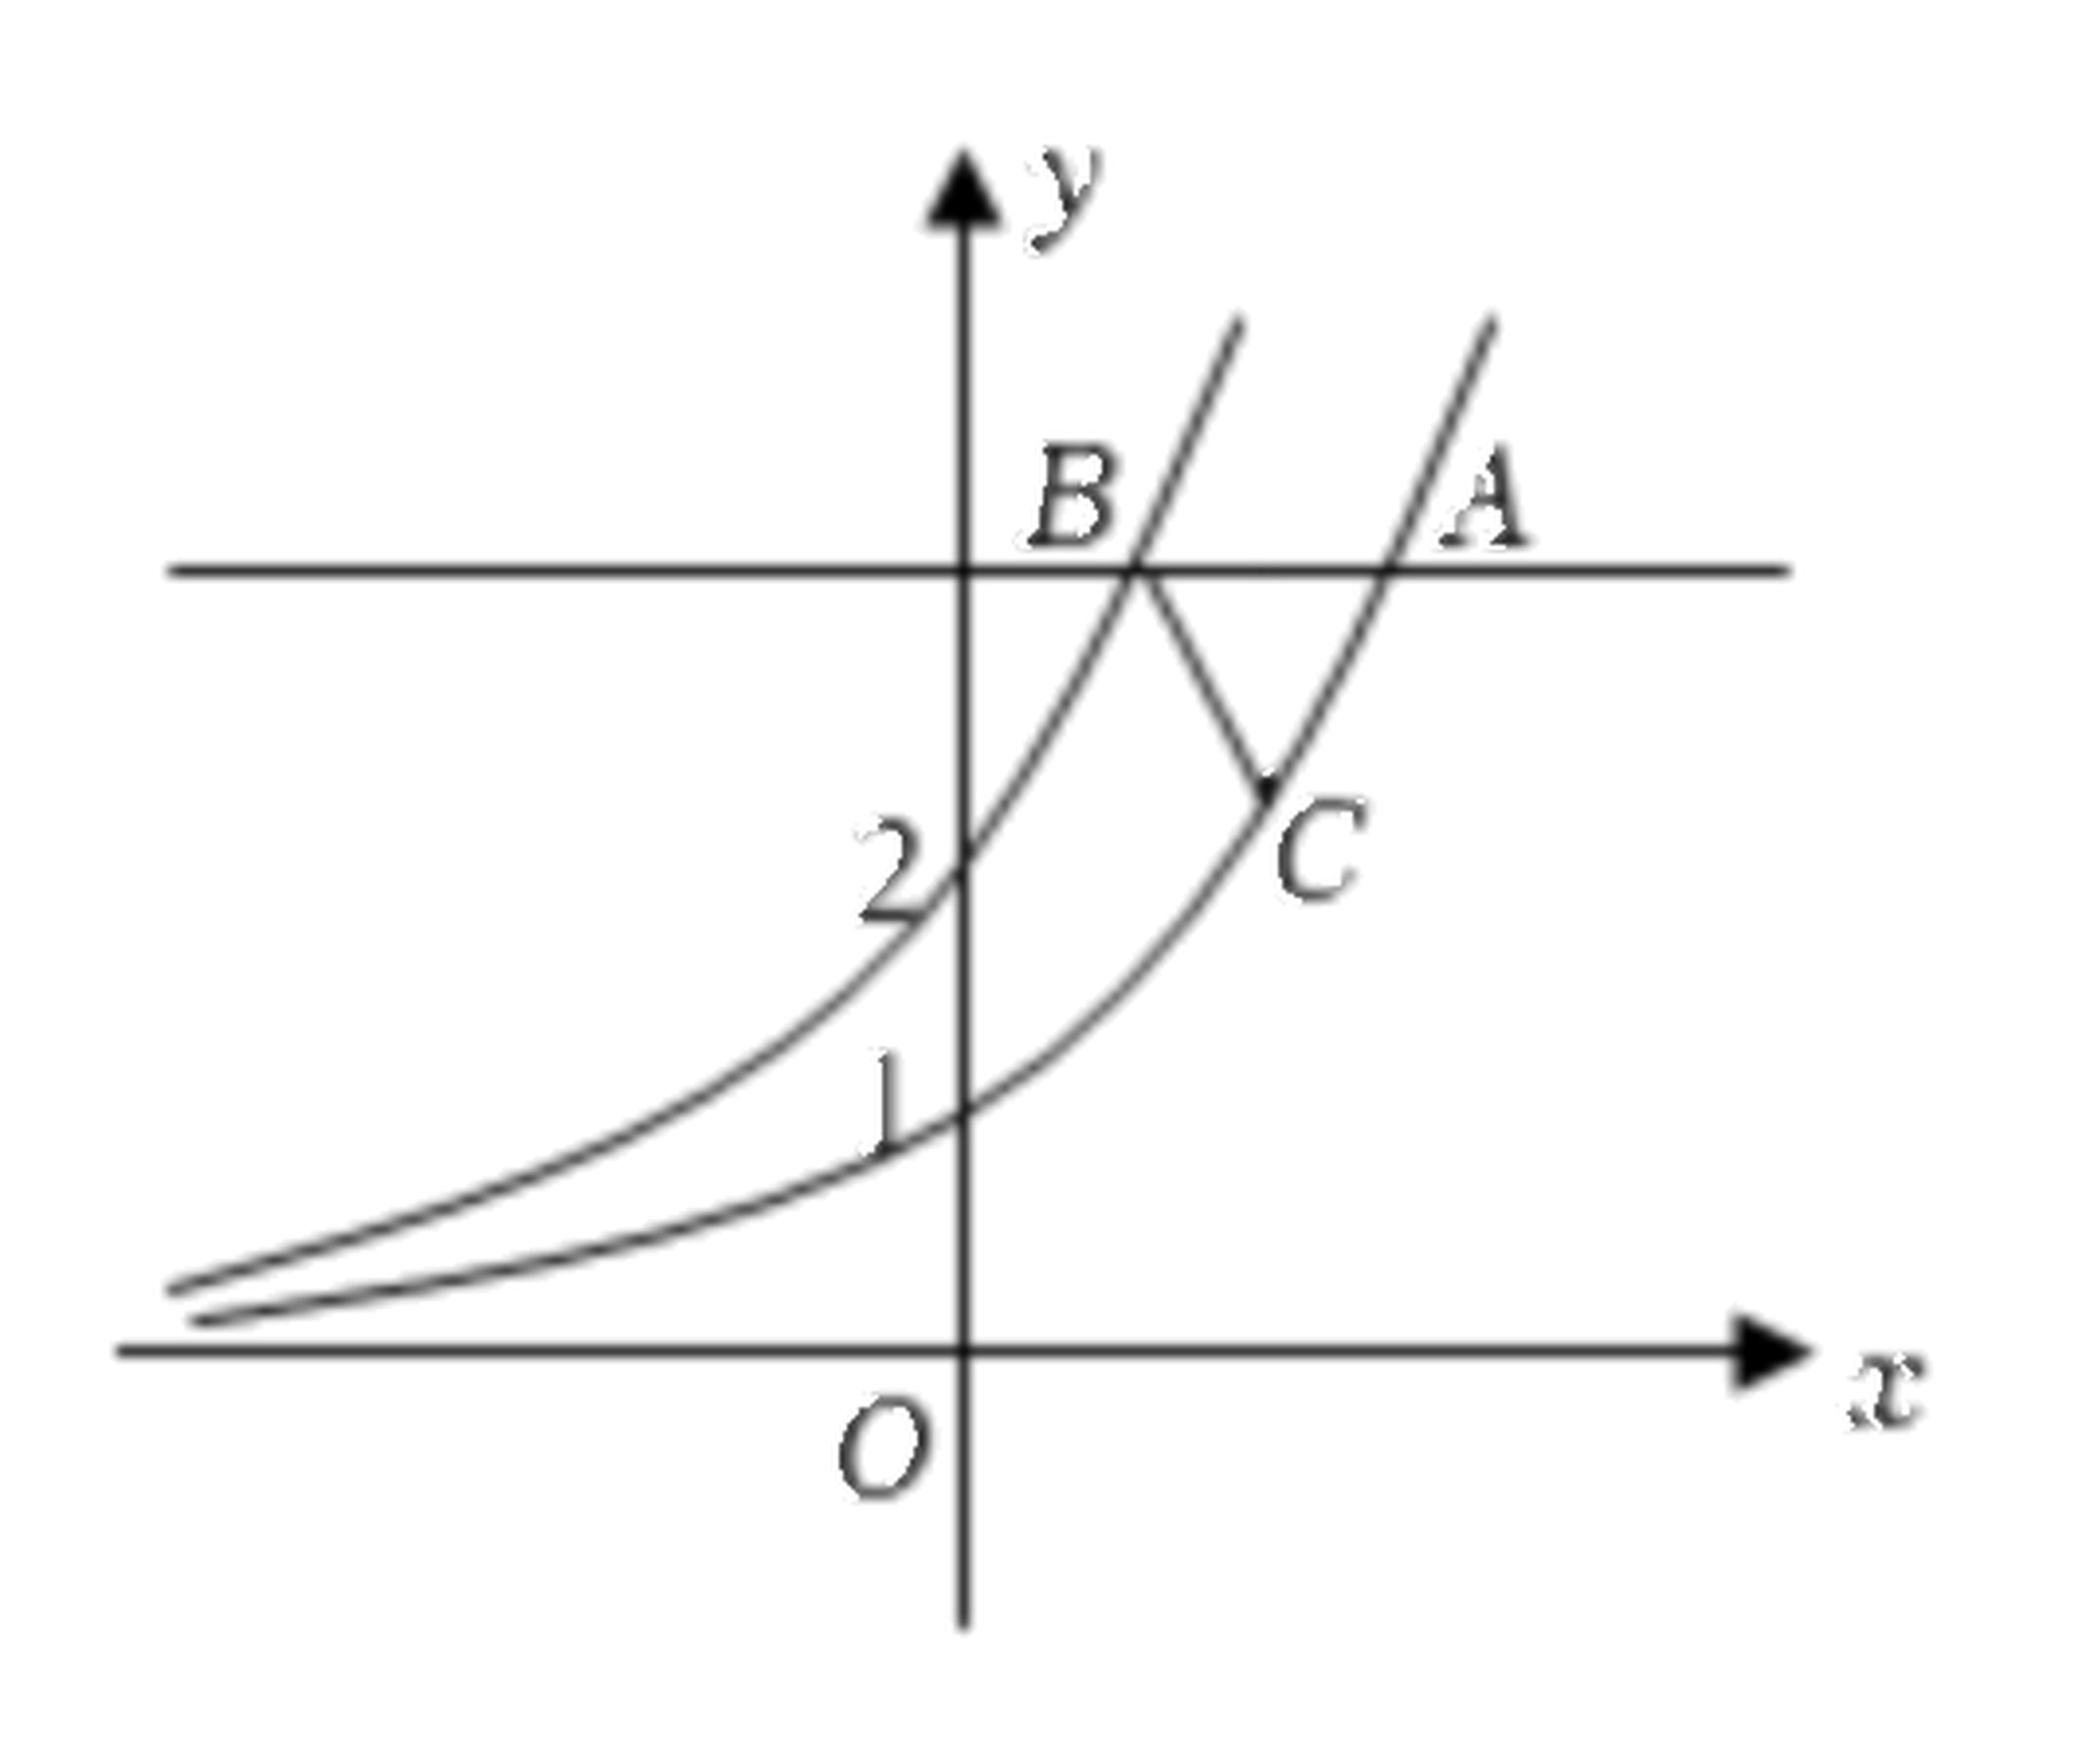
\includegraphics[width=0.40\textwidth]{figures/gao150_q11.png}
\end{center}

\ifanswer
\solbegin
\step{设直线 $l$ 的方程为 $y=a(a>0)$，}
\step{由 $2^x=a$，得 $x=\log_2 a$，所以 $A(\log_2 a,a)$，}
\step{由 $2^{x+1}=a$，得 $x=\log_2 a-1$，所以 $B(\log_2 a-1,a)$，所以 $\lvert AB\rvert=1$，}
\step{取 $AB$ 的中点 $D$，连接 $CD$，如图所示，}
\step{因为 $\triangle ABC$ 为等边三角形，则 $CD\perp AB$，且 $\lvert CD\rvert=\dfrac{\sqrt3}{2}$，}
\step{所以 $C\left(\log_2 a-\dfrac{1}{2},a-\dfrac{\sqrt3}{2}\right)$，}
\step{因为点 $C$ 在函数 $y=2^x$ 的图像上，所以 $a-\dfrac{\sqrt3}{2}=2^{\log_2 a-\frac{1}{2}}=\dfrac{a}{\sqrt2}$，}
\step{解得 $a=\dfrac{\sqrt3}{2-\sqrt2}=\dfrac{\sqrt3(2+\sqrt2)}{4-2}=\sqrt3+\dfrac{\sqrt6}{2}$，}
\step{所以点 $C$ 的纵坐标为 $a-\dfrac{\sqrt3}{2}=\dfrac{\sqrt3+\sqrt6}{2}$.}
\solend
\fi

% === Q12 === 解析配图（高斯函数方格阴影，仅答案版出）；"数学王子"弯引号；cases 块整体算一个印刷行；解析 4 行
\item 小玲在研究数学发展史，特别崇拜近代数学奠基者之一、享有“数学王子”称号的德国数学家高斯. 为了纪念高斯，我们把取整函数 $y=[x]$ 称为高斯函数，其中 $[x]$ 表示不超过 $x$ 的最大整数，如 $[1.1]=1$，$[-1.1]=-2$，则点集 $P=\{(x,y)\mid [x]^2+[y]^2=1\}$ 所表示的平面区域的面积为\blankline[4.4em].

\ifanswer
\solbegin
\step{$[x]^2+[y]^2=1$ 由 $\begin{cases}[x]=0\\ {[y]=-1}\end{cases}$ 或 $\begin{cases}[x]=0\\ {[y]=1}\end{cases}$ 或 $\begin{cases}[x]=-1\\ {[y]=0}\end{cases}$ 或 $\begin{cases}[x]=1\\ {[y]=0}\end{cases}$ 四个平面区域组成，}
\step{即 $\begin{cases}0\leqslant x<1\\ -1\leqslant y<0\end{cases}$ 或 $\begin{cases}0\leqslant x<1\\ 1\leqslant y<2\end{cases}$ 或 $\begin{cases}-1\leqslant x<0\\ 0\leqslant y<1\end{cases}$ 或 $\begin{cases}1\leqslant x<2\\ 0\leqslant y<1\end{cases}$，}
\step{作出平面区域如图所示，平面区域由四个边长为 $1$ 的正方形组成，}
\begin{center}
% 高斯函数 [x]^2+[y]^2=1 方格阴影区域图取 04 页顶部，去粉色水印、去色、4× LANCZOS 放大；仅答案版出
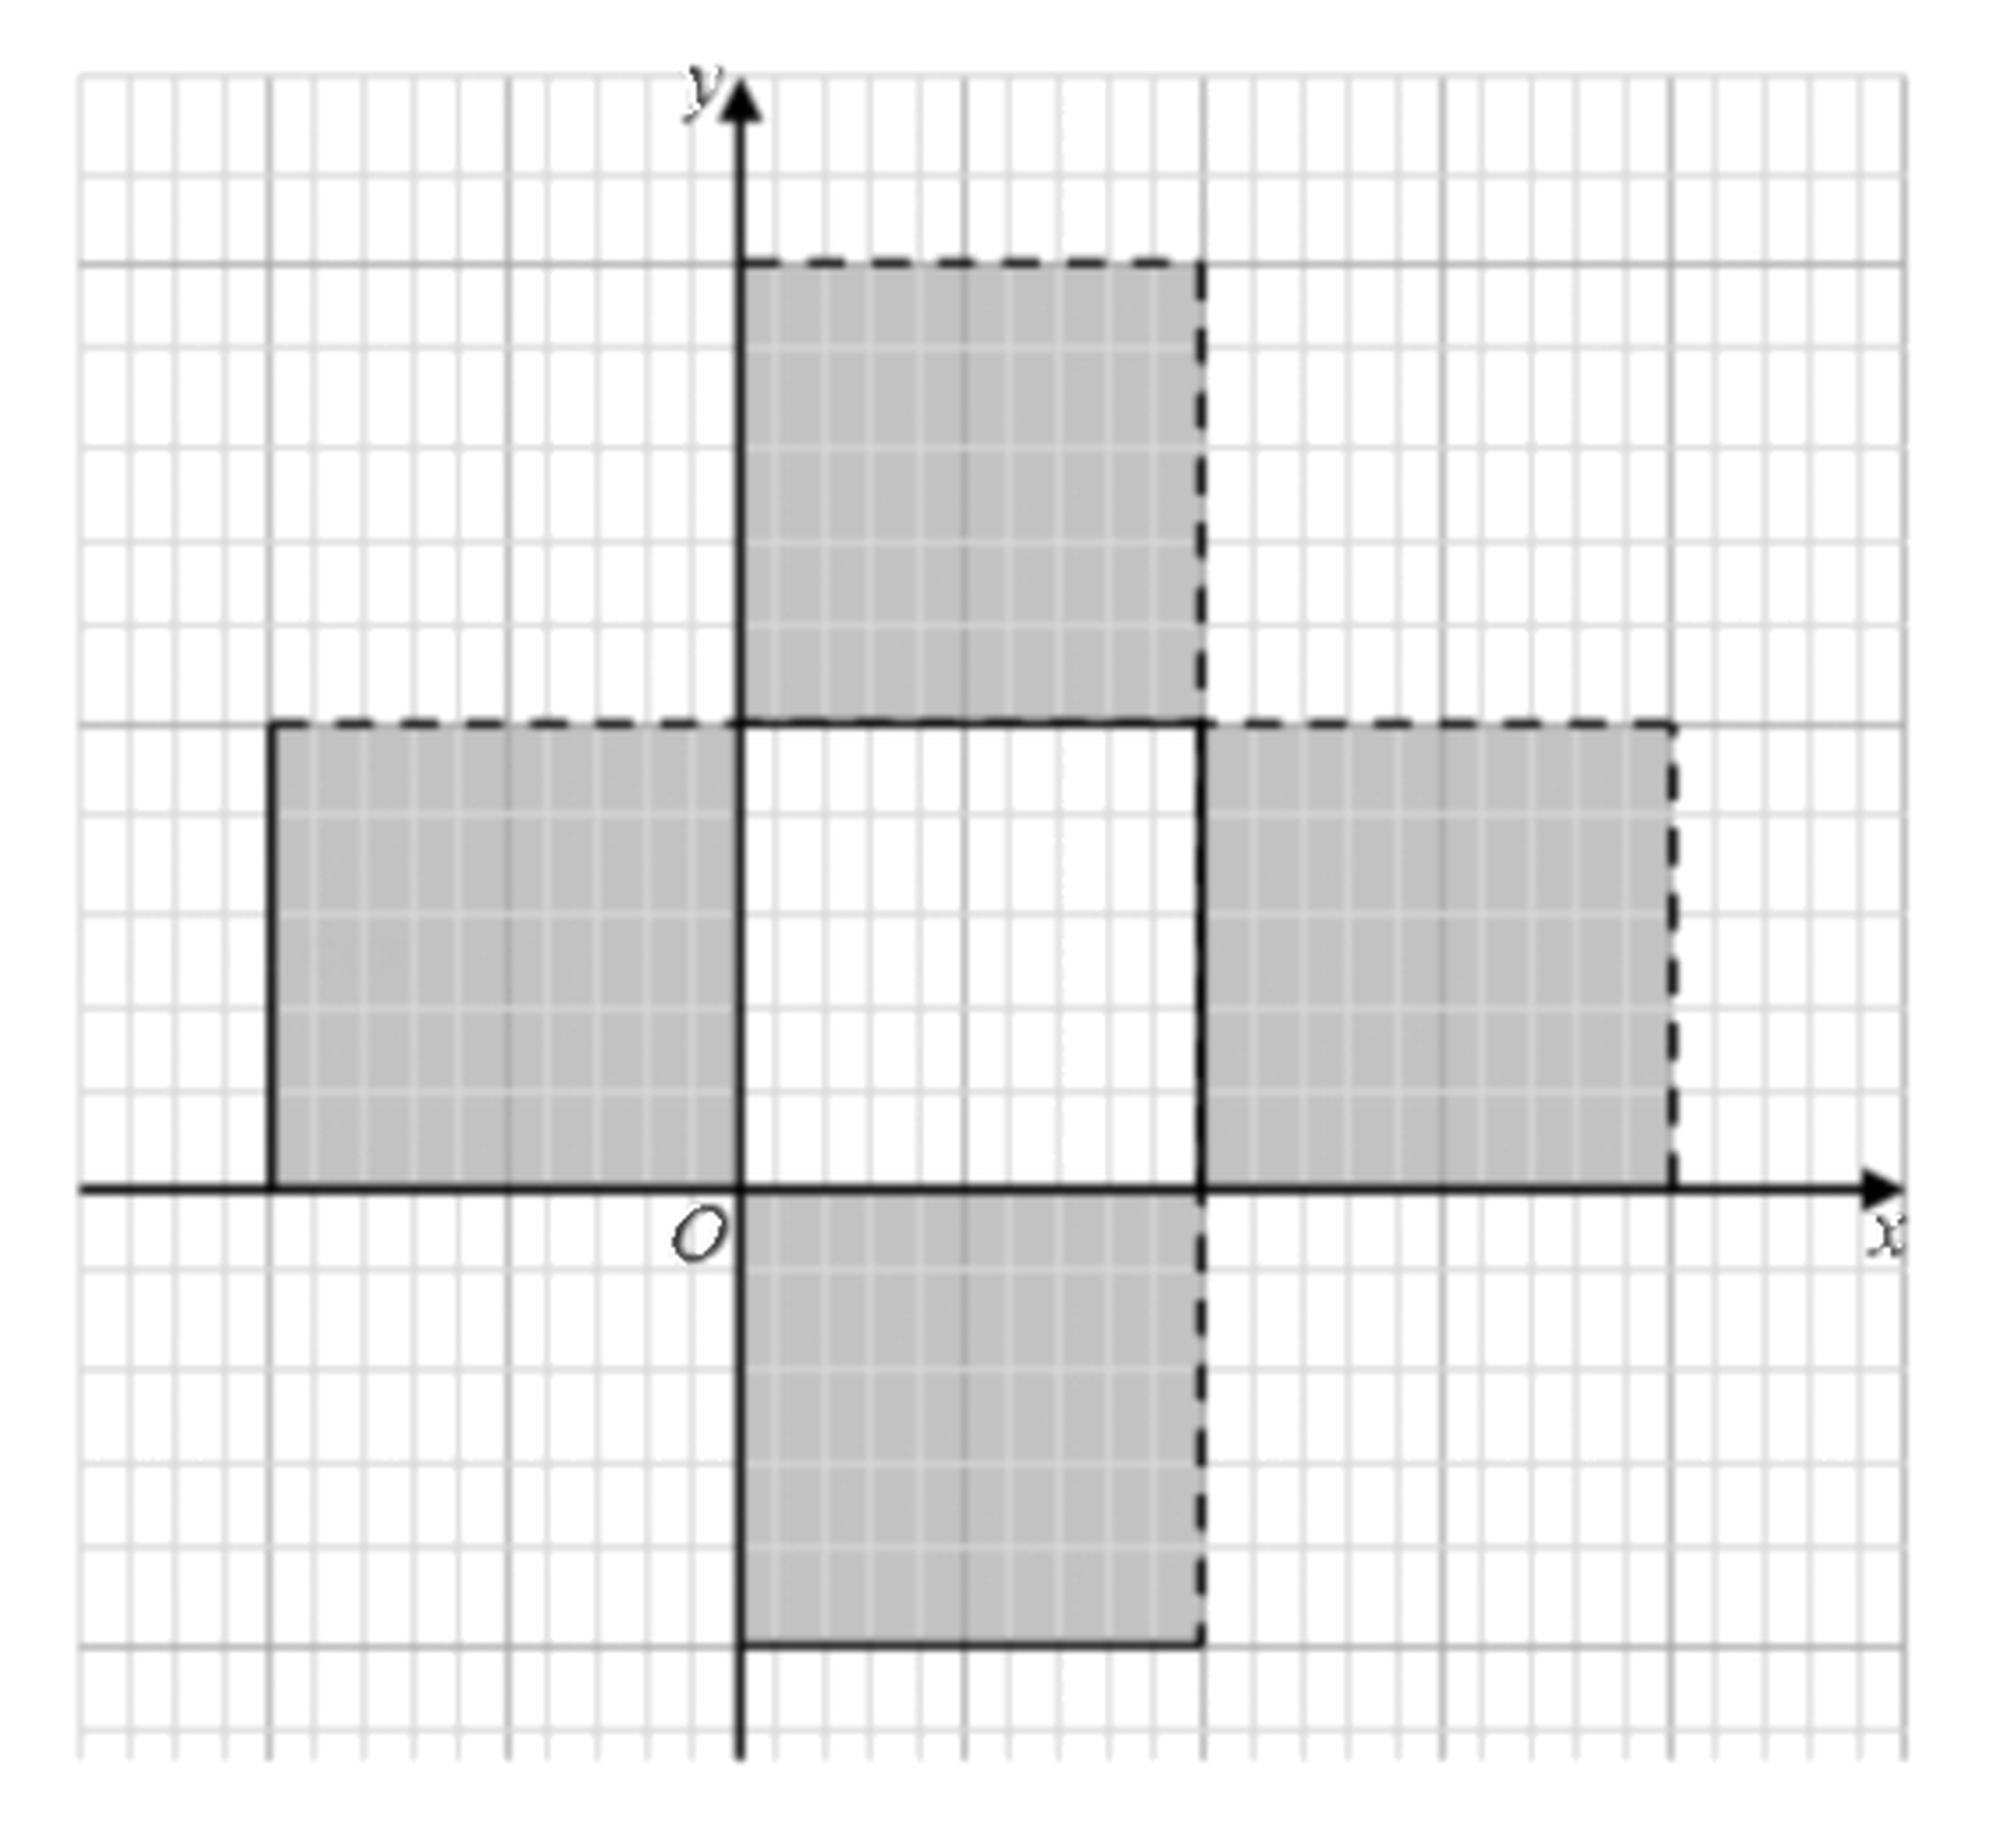
\includegraphics[width=0.34\textwidth]{figures/gao150_q12.png}
\end{center}
\step{总面积为 $1\times4=4$.}
\solend
\fi

\end{enumerate}

\bigsec{二、选择题}

\begin{enumerate}
\setcounter{enumi}{12}

% === Q13 === 答案在解析末句"故选 C"；括号 \mbox{（\quad）} 留空；四选项一行；解析 1 行
\item 设 $x\ne0$，则 $3^{\log_9 x^2}$ 的化简结果是\mbox{（\quad）}

\keepwithprev
A. $x$\qquad B. $\dfrac{1}{x}$\qquad C. $\lvert x\rvert$\qquad D. $\dfrac{1}{\lvert x\rvert}$

\ifanswer
\solbegin
\step{$3^{\log_9 x^2}=3^{\log_3\lvert x\rvert}=\lvert x\rvert$，故选 $C$.}
\solend
\fi

% === Q14 === 题目配图（两函数图像，三版都出）；\needvspace{8cm} 守卫放 \item 之前；"图像"照录；四选项两行两列；解析 2 行，故选 B
\needvspace{8cm}
\item 设 $a>0$ 且 $a\ne1$，$b\in\R$. 若函数 $y=a^{-\lvert x\rvert}$ 与 $y=x^b$ 的大致图像如图所示，则\mbox{（\quad）}

\keepwithprev
A. $0<a<1<b$\qquad\qquad B. $a>1$ 且 $b>1$

C. $0<a<1$ 且 $0<b<1$\qquad\qquad D. $0<b<1<a$

\begin{center}
% 两函数 y=a^{-|x|} 与 y=x^b 大致图像取 04 页右侧，去粉色水印、去色、4× LANCZOS 放大；三版都出
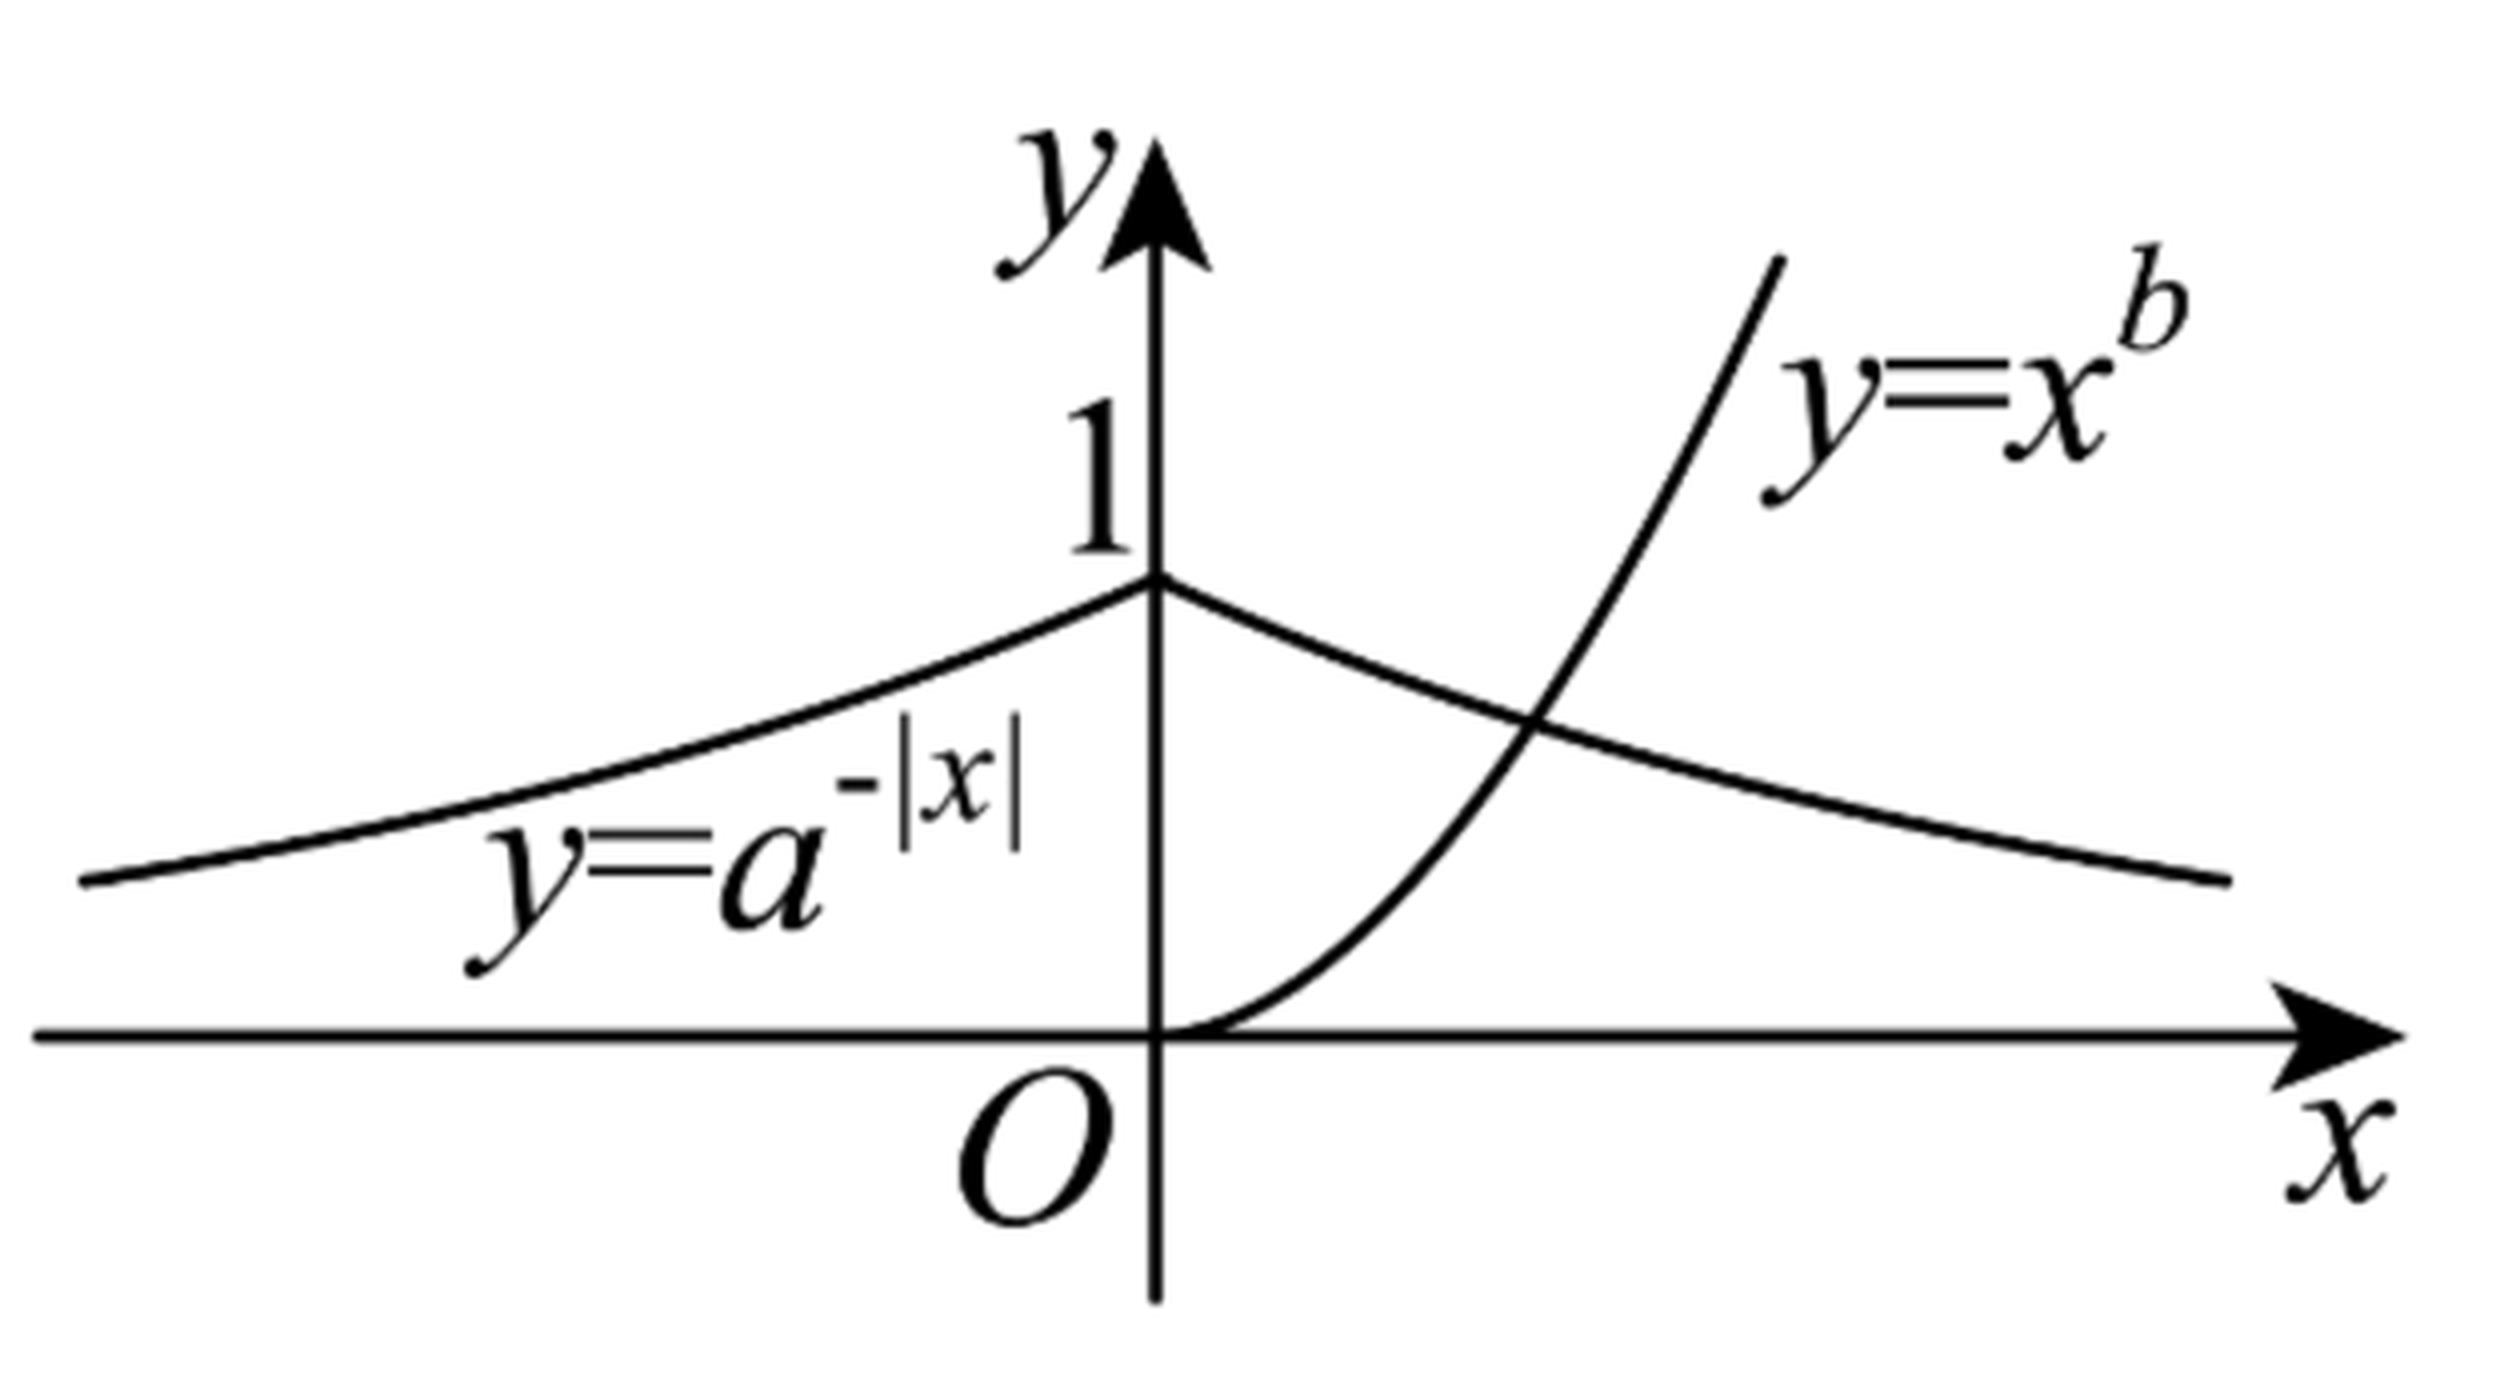
\includegraphics[width=0.40\textwidth]{figures/gao150_q14.png}
\end{center}

\ifanswer
\solbegin
\step{在 $(0,+\infty)$ 上，$y=a^{-x}$ 严格递减，得 $a>1$；}
\step{幂函数 $y=x^b$ 的图像递增且向上弯曲，得 $b>1$；故选 $B$.}
\solend
\fi

% === Q15 === "算术平均值／算术平均数"两处不同照录；四选项两行两列；解析 5 行（续 05 页顶），故选 B
\item 已知两个正数的算术平均值不小于它们的几何平均值，类比有以下结论：三个正数的算术平均数不小于它们的几何平均数，即当 $a,b,c$ 为正实数时，$\dfrac{a+b+c}{3}\geqslant\sqrt[3]{abc}$，当且仅当 $a=b=c$ 时等号成立. 利用上述结论，下列选项中判断正确的是\mbox{（\quad）}

\keepwithprev
A. 若 $x>0$，则 $2x+\dfrac{1}{x^2}\geqslant\dfrac{27}{8}$\qquad\qquad B. 若 $x>0$，则 $x^2+\dfrac{2}{x}\geqslant3$

C. 若 $0<x<1$，则 $x^2(1-x)\geqslant\dfrac{1}{9}$\qquad\qquad D. 若 $0<x<1$，则 $x^2(1-x)\leqslant\dfrac{1}{9}$

\ifanswer
\solbegin
\step{A：取 $x=1$，$2x+\dfrac{1}{x^2}=3<\dfrac{27}{8}$，错误.}
\step{B：$x^2+\dfrac{2}{x}=x^2+\dfrac{1}{x}+\dfrac{1}{x}\geqslant3\sqrt[3]{x^2\cdot\dfrac{1}{x}\cdot\dfrac{1}{x}}=3$，当且仅当 $x=1$ 时取等号，正确.}
\step{C：取 $x=\dfrac{1}{3}$，$x^2(1-x)=\dfrac{2}{27}<\dfrac{1}{9}$，错误.}
\step{D：取 $x=\dfrac{2}{3}$，$x^2(1-x)=\dfrac{4}{27}>\dfrac{1}{9}$，错误.}
\step{故选 $B$.}
\solend
\fi

% === Q16 === "完美集"新定义（弯引号、引号外空格照录）；圈数字①②文本模式；$n\in\N$；四选项两行两列；解析 9 行（6 行 05 页＋3 行 06 页顶），故选 A
\item 已知有限集 $A=\{a_1,a_2,\cdots,a_n\}$（$n\geqslant2$，$n\in\N$）. 若 $A$ 中元素 $a_i$（$i=1,2,\cdots,n$）满足 $a_1+a_2+\cdots+a_n=a_1\cdot a_2\cdots a_n$，就称 $A$ 为 “完美集”. 现有以下两个命题：

①恰有两个元素的 “完美集” 有无穷多个；

②若 $a_i$ 均为正整数，则 “完美集” $A$ 有且只有一个，且 $n=3$.

则\mbox{（\quad）}

\keepwithprev
A. ①和②都是真命题\qquad\qquad B. ①和②都是假命题

C. ①是真命题，②是假命题\qquad\qquad D. ①是假命题，②是真命题

\ifanswer
\solbegin
\step{①由 $a+b=ab\Leftrightarrow(a-1)(b-1)=1$，任取 $a>2$，则 $b=1+\dfrac{1}{a-1}\in(1,2)$，}
\step{得到无穷多个不同的完美集，①真.}
\step{②设 $1\leqslant a_1<a_2<\cdots<a_n$，则 $a_i\geqslant i$.}
\step{若 $n=2$，则 $(a_1-1)(a_2-1)=1$，只能有 $a_1=a_2=2$，与元素互异矛盾.}
\step{若 $n\geqslant4$，则 $a_1a_2\cdots a_n\geqslant a_2a_{n-1}a_n\geqslant2(n-1)a_n>na_n\geqslant a_1+\cdots+a_n$，矛盾.}
\step{当 $n=3$ 时，若 $a_1\geqslant2$，则 $a_1a_2a_3\geqslant6a_3>3a_3\geqslant a_1+a_2+a_3$，矛盾.}
\step{因此 $a_1=1$，$(a_2-1)(a_3-1)=2$，结合 $a_2<a_3$ 得 $a_2=2$，$a_3=3$.}
\step{唯一的完美集为 $\{1,2,3\}$，②真.}
\step{故选 $A$.}
\solend
\fi

\end{enumerate}

\bigsec{三、解答题}

\begin{enumerate}
\setcounter{enumi}{16}

% === Q17 === \varnothing 空集、$B\subseteq A$ 带下划线照录；弯引号内空格照录；解析 7 行
\item 设 $a,b\in\R$. 已知集合 $A=\{x\mid ax^2+3x-a>3\}$，$B=\{x\mid bx=1\}$.

(1) 若 $A=(1,2)$，求 $a$ 的值；

(2) 若 $a=0$，且 “ $x\in A$ ” 是 “ $x\in B$ ” 的必要非充分条件，求 $b$ 的取值范围.

\ifanswer
\solbegin
\step{(1) $A=(1,2)$，则 $a<0$，且 $1,2$ 是方程 $ax^2+3x-a-3=0$ 的两根.}
\step{由 $4a+6-a-3=0$，得 $a=-1$，此时不等式为 $-(x-1)(x-2)>0$，}
\step{解集确为 $(1,2)$.}
\step{(2) $a=0$ 时，$A=(1,+\infty)$，题意等价于 $B\subseteq A$ 且 $B\ne A$.}
\step{当 $b=0$ 时，$B=\varnothing$，符合条件.}
\step{当 $b\ne0$ 时，$B=\left\{\dfrac{1}{b}\right\}$，条件等价于 $\dfrac{1}{b}>1$，解得 $0<b<1$.}
\step{因此 $b$ 的取值范围为 $[0,1)$.}
\solend
\fi

% === Q18 === $p\in\Z$；"图像"（像，有亻）照录；指数 $-2p^2+5p$；解析 8 行（(1) 首行 06 页末＋2 行 07 页顶、(2) 5 行 07 页）
\item 设 $p\in\Z$，已知 $f(x)=x^{-2p^2+5p}$.

(1) 若幂函数 $y=f(x)$ 的图像关于原点成中心对称，且满足 $f(3)<f(4)$，求 $p$ 的值；

(2) 当 $p=-2$ 时，求满足 $f(2x+3)<f(x-4)$ 的 $x$ 的取值范围.

\ifanswer
\solbegin
\step{(1) 图像关于原点成中心对称，得整数 $-2p^2+5p$ 为奇数.}
\step{由 $f(3)<f(4)$，得 $-2p^2+5p>0\Leftrightarrow0<p<\dfrac{5}{2}$，}
\step{结合 $p\in\Z$，得 $p=1$ 或 $p=2$，对应指数分别为 $3$、$2$，所以 $p=1$.}
\step{(2) 当 $p=-2$ 时，$f(x)=\dfrac{1}{x^{18}}$，定义域为 $\{x\in\R\mid x\ne0\}$.}
\step{原不等式要求 $x\ne-\dfrac{3}{2}$ 且 $x\ne4$，}
\step{此时 $\dfrac{1}{(2x+3)^{18}}<\dfrac{1}{(x-4)^{18}}\Leftrightarrow\lvert 2x+3\rvert>\lvert x-4\rvert\Leftrightarrow(2x+3)^2>(x-4)^2$，}
\step{因此 $(x+7)(3x-1)>0\Leftrightarrow x<-7$ 或 $x>\dfrac{1}{3}$，}
\step{排除 $x=4$，得 $x\in(-\infty,-7)\cup\left(\dfrac{1}{3},4\right)\cup(4,+\infty)$.}
\solend
\fi

% === Q19 === $a\in\R$、$g(x)=f(2x+1)+a\cdot f(x)+2$；解析 6 行（(2) 末两行续 08 页顶）
\item 已知 $f(x)=2^x$.

(1) 求方程 $f(2x)-f(x)=6$ 的解；

(2) 设 $a\in\R$，$g(x)=f(2x+1)+a\cdot f(x)+2$，若对于任意 $x\in[-1,1]$，均有 $g(x)\geqslant1$，求 $a$ 的取值范围.

\ifanswer
\solbegin
\step{(1) 令 $t=2^x>0$，则 $t^2-t-6=(t-3)(t+2)=0$，}
\step{由 $t>0$ 得 $t=3$，所以 $x=\log_2 3$.}
\step{(2) 令 $t=2^x$，则 $t\in\left[\dfrac{1}{2},2\right]$，且 $g(x)\geqslant1\Leftrightarrow2t^2+at+1\geqslant0\Leftrightarrow a\geqslant-\left(2t+\dfrac{1}{t}\right)$，}
\step{由基本不等式得 $2t+\dfrac{1}{t}\geqslant2\sqrt{2t\cdot\dfrac{1}{t}}=2\sqrt2$，}
\step{当且仅当 $t=\dfrac{1}{\sqrt2}\in\left[\dfrac{1}{2},2\right]$ 时等号成立，}
\step{因此 $-\left(2t+\dfrac{1}{t}\right)$ 的最大值为 $-2\sqrt2$，所求范围为 $a\in[-2\sqrt2,+\infty)$.}
\solend
\fi

% === Q20 === "极闭集"新定义、3 问，全卷末题；$M\subseteq(0,+\infty)$ 带下划线照录；自定义运算 $x*y$ 星号照录；解析 13 行（9 行 08 页＋4 行 09 页上半）
\item 对于非空实数集 $M\subseteq(0,+\infty)$，若满足以下两个条件：

① $M$ 中至少含有 $2$ 个元素，且 $1\notin M$；

②对于 $M$ 中任意两个不相等的元素 $x$、$y$，定义 $x*y=\dfrac{xy+1}{x+y}$，且 $x*y\in M$.

则称 $M$ 为 “极闭集”.

(1) 分别判断集合 $A=\left\{\dfrac{1}{2},3\right\}$ 与集合 $B=(1,+\infty)$ 是否为 “极闭集” （无需理由）；

(2) 若 $M$ 是 “极闭集”，证明：$M$ 中不可能所有元素都小于 $1$；

(3) 证明：不存在任何有限集是 “极闭集”.

\ifanswer
\solbegin
\step{(1) $A$ 不是 “极闭集”，$B$ 是 “极闭集”.}
\step{(2) 假设 $M$ 中所有元素都小于 $1$，取其中两个不相等的元素 $x$、$y$，}
\step{则 $x*y-1=\dfrac{(1-x)(1-y)}{x+y}>0$，}
\step{这与 $x*y\in M$ 且 $M$ 中所有元素都小于 $1$ 矛盾.}
\step{(3) 假设有限集 $M$ 是 “极闭集”，}
\step{由 (2) 及 $1\notin M$，得 $M$ 中存在大于 $1$ 的元素.}
\step{若 $M$ 中有小于 $1$ 的元素，取其中最大的一个为 $a$，另取 $b\in M$ 且 $b>1$，}
\step{则 $a*b-a=\dfrac{1-a^2}{a+b}>0, a*b-1=\dfrac{(a-1)(b-1)}{a+b}<0$，}% 半角逗号在两个数学式组之间，全稿惯例、非笔误，照录
\step{于是 $a<a*b<1$ 且 $a*b\in M$，与 $a$ 的最大性矛盾.}
\step{若 $M$ 中没有小于 $1$ 的元素，则 $M\subseteq(1,+\infty)$.}
\step{取 $a=\min M$，另取 $b\in M$ 且 $b\ne a$，则 $a*b-a=\dfrac{1-a^2}{a+b}<0$，}
\step{于是 $a*b<a$ 且 $a*b\in M$，与 $a$ 的最小性矛盾.}
\step{因此不存在任何有限集是 “极闭集”.}
\solend
\fi

\end{enumerate}

\end{document}
"
%
% ① 原始材料：微信公众号"魔都数学加油站"文章，连载"27学年高一150"，原文标题
% "27学年高一150——2026-2027年上海市曹杨二中高一上期中"；
% 原文链接：https://mp.weixin.qq.com/s/xlQxmik8TZXR87RC6MnCrw 。
% 正文为 9 张 PNG 页（01/02/04/06/07/09 为 2560×3620，03/05/08 为 4762×6735，
% 同一篇各页分辨率混排，逐页按各自分辨率裁图核对，别按预览比例换算裁框）。
% 体例：讲评版——全 18 题均印【解析】（逐题核实，见 ② ②）。
% 题目、答案、解析均据原图转录；卷面粉红色/红色水印"魔都数学加油站"及公众号页脚未录入。
% 全卷插图清单（逐页通读 9 页确认）：3 幅——
%   · Q11 题目配图（指数函数曲线图，02 页右侧：x/y 轴、O、y=2^x 与 y=2^{x+1}
%     两曲线、A/B/C 三点、刻度 1/2、等边三角形 ABC），三版都出，裁 figures/gao150_q11.png；
%   · Q12 解析配图（高斯函数取整 [x]^2+[y]^2=1 方格阴影区域图，04 页顶部：4 个边长 1
%     的正方形组成的十字形阴影），解析"作出平面区域如图所示"处，仅答案版出，
%     放 \ifanswer 内 \step 之间，裁 figures/gao150_q12.png；
%   · Q14 题目配图（两函数 y=a^{-|x|} 与 y=x^b 大致图像，04 页右侧：x/y 轴、O、
%     y 轴刻度 1、一递减曲线一递增上翘曲线），三版都出，裁 figures/gao150_q14.png；
%   其余各页逐页确认无其它题目配图、无表格；Q11/Q12 解析"如图所示"对应的就是上列
%   已裁的图，不重复裁；09 页上半为 Q20(3) 解析续尾、下半仅水印、无正文。
%   3 图均取自原卷截图，去粉色水印、去色、4× LANCZOS 放大。
%
% 卷首标题：原卷印作"2026-2027 年曹杨二中高一上期中"，年份区间按全稿惯例排 en dash；
% 原卷卷面未印副标题，本稿按同期中卷知识模块口径补出"集合与常用逻辑用语、不等式、函数"。
%
% 题号体例（逐页核实定稿）：本卷共 18 题——一、填空题 3—12（10 题）、
% 二、选择题 13—16（4 题）、三、解答题 17—20（4 题）。
% 三节分别 \setcounter{enumi}{2}／{12}／{16}。原卷从第 3 题起、无第 1、2 题，
% 本稿保留原题号；全卷末题为第 20 题（"极闭集"新定义、3 问），无 Q21、无附加题节。
%
% ② 与原卷的排版差异：
%   ① 原文从第 3 题起，本稿保留原题号；共 18 题三节，解答题只有 4 题到 20；
%   ② 全 18 题均印【解析】，用 \solbegin…\solend；逐题核实无只印【答案】或
%      答案印题干括号内的题；四道选择题答案在解析末句"故选 X"（Q13 选 C、
%      Q14 选 B、Q15 选 B、Q16 选 A，逐个放大复核）、括号 \mbox{（\quad）} 留空、
%      不另提 \ans{}；答案版【答案】/【解析】标记数 = 18 = 全卷题数；
%   ③ 原卷卷面未印副标题，本稿按知识模块口径补出；
%   ④ 原卷填空横线按全稿惯例排 \blankline[4.4em]；选择题括号排 \mbox{（\quad）}、
%      选项段前按惯例加 \keepwithprev；解答题不留作答区、不加 \anspace（原卷为讲评版）；
%   ⑤ 数集黑板粗体：Q4"m\in R"、Q5"a,b\in R"、Q6"a,b,c\in R"、Q7"a\in R"、
%      Q10"a\in R"、Q14"b\in R"、Q17"a,b\in R"、Q18"p\in Z"／定义域"x\in R"、
%      Q19"a\in R"、Q16"n\in N" 原卷印斜体 R/Z/N，按全稿惯例归一 \R／\Z／\N；
%      绝对值排 \lvert…\rvert（Q7 |x+4|+|x-3|、Q11 |AB|／|CD|、Q13 |x|、
%      Q18 |2x+3|／|x-4|），集合描述竖线排 \mid（Q3、Q12、Q17、Q18、Q20），
%      不等号按全稿惯例排 \leqslant／\geqslant；补集照原卷上划线排 \overline{A}
%      （Q3 题干＋解析共 2 处）；空集符号 \varnothing（Q17 解析(2)）；
%      子集 \subset（单线⊂）／\subseteq（带下划线⊆）逐处照录，本卷 3 处子集
%      符号均印带下划线 ⊆、照录 \subseteq（Q20 题干、Q20 解析(3)、Q17 解析(2)，
%      见 ④），无 \subset 用例；
%   ⑥ 判别式 Δ/△：逐页通读 9 页，本卷无一元二次判别式算式，故无 Δ/△ 混用可照录
%      （"高 \Delta／扁 \triangle"口径备查，参照 高一142／144／145／146／148／149
%      头注④）；本卷仅 Q11 题干与解析共 2 处几何三角形符号 △ABC，逐处放大并排
%      确认两处同形、印近等边粗线三角（非判别式），照录 \triangle（见 ④）；
%   ⑦ 中文弯引号照录：Q12"数学王子"、Q16"完美集"（题干＋①②两命题，引号外
%      留空格）、Q17" x∈A "" x∈B "（引号内空格）、Q20"极闭集"（题干条件、
%      三问与解析，引号外留空格）；注释里一律 ASCII 引号；数学式内 CJK 用 \text{}
%      （Q3 集合描述"且"用 \text{ 且 }）；
%   ⑧ 半角逗号在数学组之间是全稿惯例、非笔误，逐处照录（Q17 解析"1,2 是方程…
%      两根"、Q20 解析(3)">0, a*b-1=…<0" 两式之间等）；行末西文句点 ASCII `.`；
%      行中全角逗号／顿号照录（Q12"之一、享有"、Q18 解析"3、2"、Q20"x、y"）；
%   ⑨ "图像／图象"逐处放大核：全卷 9 处均印"图像"（像，有亻）、未见"图象"——
%      Q4 题干 1、Q11 题干 2＋解析 1、Q14 题干 1＋解析 1、Q18 题干 1＋解析 1；
%      同卷"第二象限""象限"用"象"（无亻）。逐处照录未统一改动（放大 01/02/04/06
%      页 /tmp/gao150/z/p01_q4_tuxiang2.png、p04_q14_tuxiang2.png、
%      p02_q11_lines.png 确认）；子题标号 (1)(2)(3) 半角括号照录；圈数字①②
%      在文本模式（Q16 两命题与解析、Q20 两条件与三问及解析）按 common.sty
%      划入 CJK 字符类渲染，进数学式用 \text{①}；
%   ⑩ Q20 新定义 x*y=\dfrac{xy+1}{x+y} 的 * 是自定义运算（星号），照录；
%      \left…\right 不得拆到不同 $…$ 组（Q19"\left(2t+\frac1t\right)"、
%      Q20 题干"A=\left\{\frac12,3\right\}"等）；Q8 嵌套根号
%      \sqrt{\frac2x+\frac{16}{1-2x}}、Q9 对数连加 \log_2 A 等复杂式照录别简化；
%   ⑪ 一条 \step = 原卷解析的一个印刷行，cases 块整体算一个印刷行；别并折行、
%      别拆行。Q4 三行、Q8 五行、Q11 九行、Q12 四行（两行各含四个 cases 块）、
%      Q15 五行、Q16 九行、Q18 八行、Q20 十三行均按印刷行逐条断，不丢行；
%   ⑫ 配图：Q11／Q14 题目配图（三版都出）放 \item 内题干之后 \begin{center}，
%      大图块加 \needvspace{8cm} 守卫把整块推走（守卫放 \item 之前，见
%      高一145 Q14/Q20 成例与切页审计 B 类坑）；Q12 解析配图（仅答案版出）
%      放 \ifanswer 内 \solbegin…\solend 的 \step 之间（高一73 第16题成例）；
%   ⑬ 跨页续印按题合并：见 ⑥；
%   ⑭ 原卷解析内无红色"法一／法二"之类小标题，故本卷无 \stepm；红色水印
%      "魔都数学加油站"不录入；Q12 解析"作出平面区域如图所示"对应的图即
%      ① 所列 gao150_q12.png（04 页顶部），不重复裁；Q11 解析"如图所示"对应
%      题目配图 gao150_q11.png，不另裁。
%
% ③ 行数复核：一条 \step／\stepm = 原卷解析的一个印刷行，cases 块作一个印刷行计。
%   逐题数（主会话逐页核对定稿）：Q3：1；Q4：3；Q5：2；Q6：1；Q7：2；Q8：5；
%   Q9：1；Q10：3；Q11：9；Q12：4；Q13：1；Q14：2；Q15：5；Q16：9；
%   Q17：7；Q18：8；Q19：6；Q20：13。
%   合计 82 条 \step（本卷无 \stepm：解析内无红色"法一／法二"类小标题），
%   与原卷逐题印刷行相等。全卷 18 题均设 \solbegin…\solend，答案版
%   【答案】/【解析】标记数 = 18 = 全卷题数。
%
% ④ 判别式／三角形／子集符号结论（逐处放大原图照录、不得统一，主会话像素级复核）：
%   判别式：逐页通读 9 页，本卷无一元二次判别式 Δ/△ 算式（Q18 讨论幂函数指数
%     奇偶、不用判别式；Q9／Q19／Q20 亦无），头注 ② ⑥ 的"高 \Delta／扁 \triangle"
%     口径在本卷无对应处（参照 高一142／144／145／146／148／149 头注④，仅备查）。
%   几何三角形符号：Q11 题干"使得 △ABC 为等边三角形"（02 页末）与解析
%     "因为 △ABC 为等边三角形，则 CD⊥AB"（03 页）共 2 处，放大 02/03 页
%     /tmp/gao150/z/q11_tri_montage2.png 并排确认两处同形、印近等边粗线三角
%     （h/w≈0.98、非"高>宽"的判别式 \Delta），照录 \triangle（与 高一105
%     "使得 \triangle ABC 为等边三角形" 同短语成例、高一149 几何三角形照录
%     \triangle 口径一致），不引入 \Delta。
%   子集／补集：Q20 题干"$M\subseteq(0,+\infty)$"（08 页）、Q20 解析(3)
%     "则 $M\subseteq(1,+\infty)$"（09 页）、Q17 解析(2)"题意等价于 $B\subseteq A$
%     且 $B\ne A$"（06 页）共 3 处子集符号，逐处放大（/tmp/gao150/z/p08_q20_stem.png、
%     p09_q20_sub.png、p06_q17_sub.png）确认均印带下划线 ⊆，照录 \subseteq；
%     本卷未见单线 ⊂（\subset）之对应处。Q3 题干与解析共 2 处补集照原卷上划线
%     排 \overline{A}；Q17 解析(2) 空集印 ∅、照录 \varnothing（Q7"解集为空集"
%     为中文词、非符号，照录文字）；集合描述竖线 \mid；数集 \R／\Z／\N 归一见 ② ⑤。
%
% ⑤ 存疑照录（放大原图确认，照录未改、正文对应处另有 % 注）：
%   1. Q8 解析第 4 行"所以 $y=\frac1x+\frac{8}{1-2x}$ 的最小值为 18" —— 上文
%      并未定义 $y$，且题面求的是 $\sqrt{\frac2x+\frac{16}{1-2x}}$ 的最小值；
%      按上下文该行应为 $\frac1x+\frac{8}{1-2x}$ 的最小值为 18（$y$ 疑为原卷
%      衍字／笔误），放大 02 页 /tmp/gao150/z/p02_q8_y.png 确认，照录未改。
%   2. Q20 解析(3)"$a*b-a=\frac{1-a^2}{a+b}>0, a*b-1=\frac{(a-1)(b-1)}{a+b}<0$"
%      两式之间的逗号原卷印半角 ,（非全角），按全稿惯例"半角逗号在数学组之间"
%      照录未改（放大 08 页 /tmp/gao150/z/p08_q20_sol8.png 确认）。
%   3. Q15 题干"两个正数的算术平均值…几何平均值"与"三个正数的算术平均数…
%      几何平均数"两处"值／数"用字不同，逐处照录未统一（放大 04 页确认）。
%   4. "图像／图象"全卷 9 处均印"图像"（像，有亻）、未见"图象"，逐处放大核实
%      照录、未统一改动（见 ② ⑨）；本卷判别式 Δ/△ 无用例、几何三角形 2 处
%      照录 \triangle（见 ④）。
%   全卷除此 4 类外未发现其它笔误／自相矛盾处；18 题均印【解析】、无只印【答案】
%   或答案印题干括号内的题（见 ② ②）。
%
% ⑥ 跨页续印按题合并说明（逐页核实定稿）：Q3/4/5/6/7 题干＋解析在 01 页；
%   Q8 题干＋解析 5 行、Q9 题干＋解析 1 行在 02 页上半；Q10 题干＋解析 3 行
%   在 02 页下半；Q11 题干（前两行）＋配图在 02 页下半、题干续"三角形，则点 C
%   的纵坐标为___"与解析 9 行全在 03 页上半（解析"如图所示"对应题目配图）；
%   Q12 题干＋解析 4 行在 03 页下半，解析配图（方格阴影）续印在 04 页顶部；
%   "二、选择题"标题在 04 页中部；Q13 题干＋选项＋解析、Q14 题干＋选项＋
%   配图＋解析在 04 页；Q15 题干＋四选项在 04 页末、解析 5 行续 05 页上半；
%   Q16 题干＋①②两命题＋"则(  )"＋四选项＋解析前 6 行在 05 页、解析末 3 行
%   （"因此 a_1=1…②真""故选 A"）续 06 页顶部；"三、解答题"标题在 06 页；
%   Q17 题干(1)(2)＋解析(1) 3 行＋解析(2) 首行在 06 页、解析(2) 续 3 行
%   在 06 页下半；Q18 题干(1)(2)＋解析(1) 首行在 06 页末、解析(1) 续 2 行＋
%   解析(2) 5 行在 07 页上半；Q19 题干(1)(2)＋解析(1) 2 行＋解析(2) 前 2 行
%   在 07 页下半、解析(2) 末 2 行续 08 页顶部；Q20 题干（新定义＋①②两条件）
%   ＋三问＋解析(1)(2)(3) 前 9 行在 08 页、解析(3) 末 4 行续 09 页上半，
%   末行"因此不存在任何有限集是极闭集"为全卷收尾（09 页下半仅水印、无正文）。
%   本稿按题连排，不丢行、不并折行；全卷末题为第 20 题，无 Q21、无附加题节。
%
\documentclass[a4paper,11pt]{article}
\usepackage{common}

\begin{document}

\examtitlest[3]{2026--2027 年曹杨二中高一上期中}{集合与常用逻辑用语、不等式、函数}

\bigsec{一、填空题}

\begin{enumerate}
\setcounter{enumi}{2}

% === Q3 === 补集上划线 \overline{A}（题干＋解析各 1 处）；集合描述竖线 \mid、数学式内"且"用 \text{}；解析 1 行
\item 设全集 $U=\{1,2,3,4,5\}$，集合 $A=\{x\mid x^2-3x\leqslant0\text{ 且 }x\in U\}$，则 $\overline{A}=$\blankline[4.4em].

\ifanswer
\solbegin
\step{$x^2-3x\leqslant0\Leftrightarrow0\leqslant x\leqslant3$，所以 $A=\{1,2,3\}$，$\overline{A}=\{4,5\}$.}
\solend
\fi

% === Q4 === "图像"（像，有亻）逐处照录、同句"第二象限"用"象"（无亻）；解析 3 行
\item 设 $m\in\R$. 若幂函数 $y=(m^2-5m+1)x^{m+1}$ 的图像经过第二象限，则 $m=$\blankline[4.4em].

\ifanswer
\solbegin
\step{幂函数的系数为 1，故 $m^2-5m+1=1\Rightarrow m=0$ 或 $m=5$.}
\step{$m=0$ 时，$y=x$ 不经过第二象限；}
\step{$m=5$ 时，$y=x^6$ 经过第二象限，因此 $m=5$.}
\solend
\fi

% === Q5 === 解析 2 行
\item 设 $a,b\in\R$. 若 $a^2+\dfrac{b^2}{4}=1$，则 $ab$ 的最大值为\blankline[4.4em].

\ifanswer
\solbegin
\step{$1-ab=\left(a-\dfrac{b}{2}\right)^2\geqslant0$，即 $ab\leqslant1$；}
\step{当 $a=\dfrac{\sqrt2}{2}$，$b=\sqrt2$ 时取等号，最大值为 1.}
\solend
\fi

% === Q6 === 解析 1 行
\item 设 $a,b,c\in\R$. 若等式 $2x^2-3x-2=a(x-1)^2+b(x-1)+c$ 恒成立，则 $a-b+c=$\blankline[4.4em].

\ifanswer
\solbegin
\step{令 $x=0$，得 $a-b+c=-2$.}
\solend
\fi

% === Q7 === 绝对值 \lvert…\rvert；解析 2 行
\item 设 $a\in\R$. 若关于 $x$ 的不等式 $\lvert x+4\rvert+\lvert x-3\rvert<a$ 的解集为空集，则 $a$ 的取值范围是\blankline[4.4em].

\ifanswer
\solbegin
\step{$\lvert x+4\rvert+\lvert x-3\rvert\geqslant\lvert(x+4)-(x-3)\rvert=7$，当 $-4\leqslant x\leqslant3$ 时取等号.}
\step{原不等式的解集为空集当且仅当 $a\leqslant7$，即 $a\in(-\infty,7]$.}
\solend
\fi

% === Q8 === 嵌套根号 \sqrt{\frac{2}{x}+\frac{16}{1-2x}} 照录别简化；解析 5 行
\item 设 $x\in\left(0,\dfrac{1}{2}\right)$，则 $\sqrt{\dfrac{2}{x}+\dfrac{16}{1-2x}}$ 的最小值为\blankline[4.4em].

\ifanswer
\solbegin
\step{因为 $x\in\left(0,\dfrac{1}{2}\right)$，所以 $1-2x>0$，又 $2x+1-2x=1$，}
\step{所以 $\left(\dfrac{1}{x}+\dfrac{8}{1-2x}\right)(2x+1-2x)=10+\dfrac{1-2x}{x}+\dfrac{16x}{1-2x}$}
\step{$\geqslant10+2\sqrt{\dfrac{1-2x}{x}\cdot\dfrac{16x}{1-2x}}=18$，}
\step{当且仅当 $\dfrac{1-2x}{x}=\dfrac{16x}{1-2x}$ 即 $x=\dfrac{1}{6}$ 时取等号，所以 $y=\dfrac{1}{x}+\dfrac{8}{1-2x}$ 的最小值为 18，}% 原卷此处径写 $y=\frac1x+\frac{8}{1-2x}$（上文未定义 $y$、且与题面根式不符），疑笔误，放大 02 页确认，照录未改（见 ⑤）
\step{所以 $\sqrt{\dfrac{2}{x}+\dfrac{16}{1-2x}}$ 的最小值为 6.}
\solend
\fi

% === Q9 === 对数连加 \log_2 A 等复杂式照录别简化；解析 1 行
\item 记 $A=1\times2\times3\times\cdots\times2026$，则 $\dfrac{1}{\log_2 A}+\dfrac{1}{\log_3 A}+\dfrac{1}{\log_4 A}+\cdots+\dfrac{1}{\log_{2026}A}=$\blankline[4.4em].

\ifanswer
\solbegin
\step{原式 $=\log_A 2+\cdots+\log_A 2026=\log_A(2\times3\times\cdots\times2026)=\log_A A=1$.}
\solend
\fi

% === Q10 === "严格减函数／不恒为负／⇔"照录；解析 3 行
\item 设 $a\in\R$，$f(x)=\dfrac{ax+1}{x+2}$. 若函数 $y=f(x)$ 在 $[1,+\infty)$ 上是严格减函数，且在 $[1,+\infty)$ 上的函数值不恒为负，则 $a$ 的取值范围是\blankline[4.4em].

\ifanswer
\solbegin
\step{当 $1\leqslant x_1<x_2$ 时，$f(x_2)-f(x_1)=\dfrac{(2a-1)(x_2-x_1)}{(x_1+2)(x_2+2)}$，故严格递减 $\Leftrightarrow a<\dfrac{1}{2}$.}
\step{此时最大函数值为 $f(1)$，函数值不恒为负 $\Leftrightarrow f(1)=\dfrac{a+1}{3}\geqslant0\Leftrightarrow a\geqslant-1$，}
\step{得 $a\in\left[-1,\dfrac{1}{2}\right)$.}
\solend
\fi

% === Q11 === 题目配图（指数函数曲线，三版都出）；\needvspace{8cm} 守卫放 \item 之前；"图像"照录、几何三角形 \triangle；解析 9 行（全在 03 页）
\needvspace{8cm}
\item 如图，点 $C$ 是函数 $y=2^x$ 的图像上的一点，若存在平行于 $x$ 轴的直线 $l$ 分别与函数 $y=2^x$ 和 $y=2^{x+1}$ 的图像相交于点 $A$、$B$，使得 $\triangle ABC$ 为等边三角形，则点 $C$ 的纵坐标为\blankline[4.4em].

\begin{center}
% 指数函数曲线图取 02 页右侧，去粉色水印、去色、4× LANCZOS 放大；三版都出
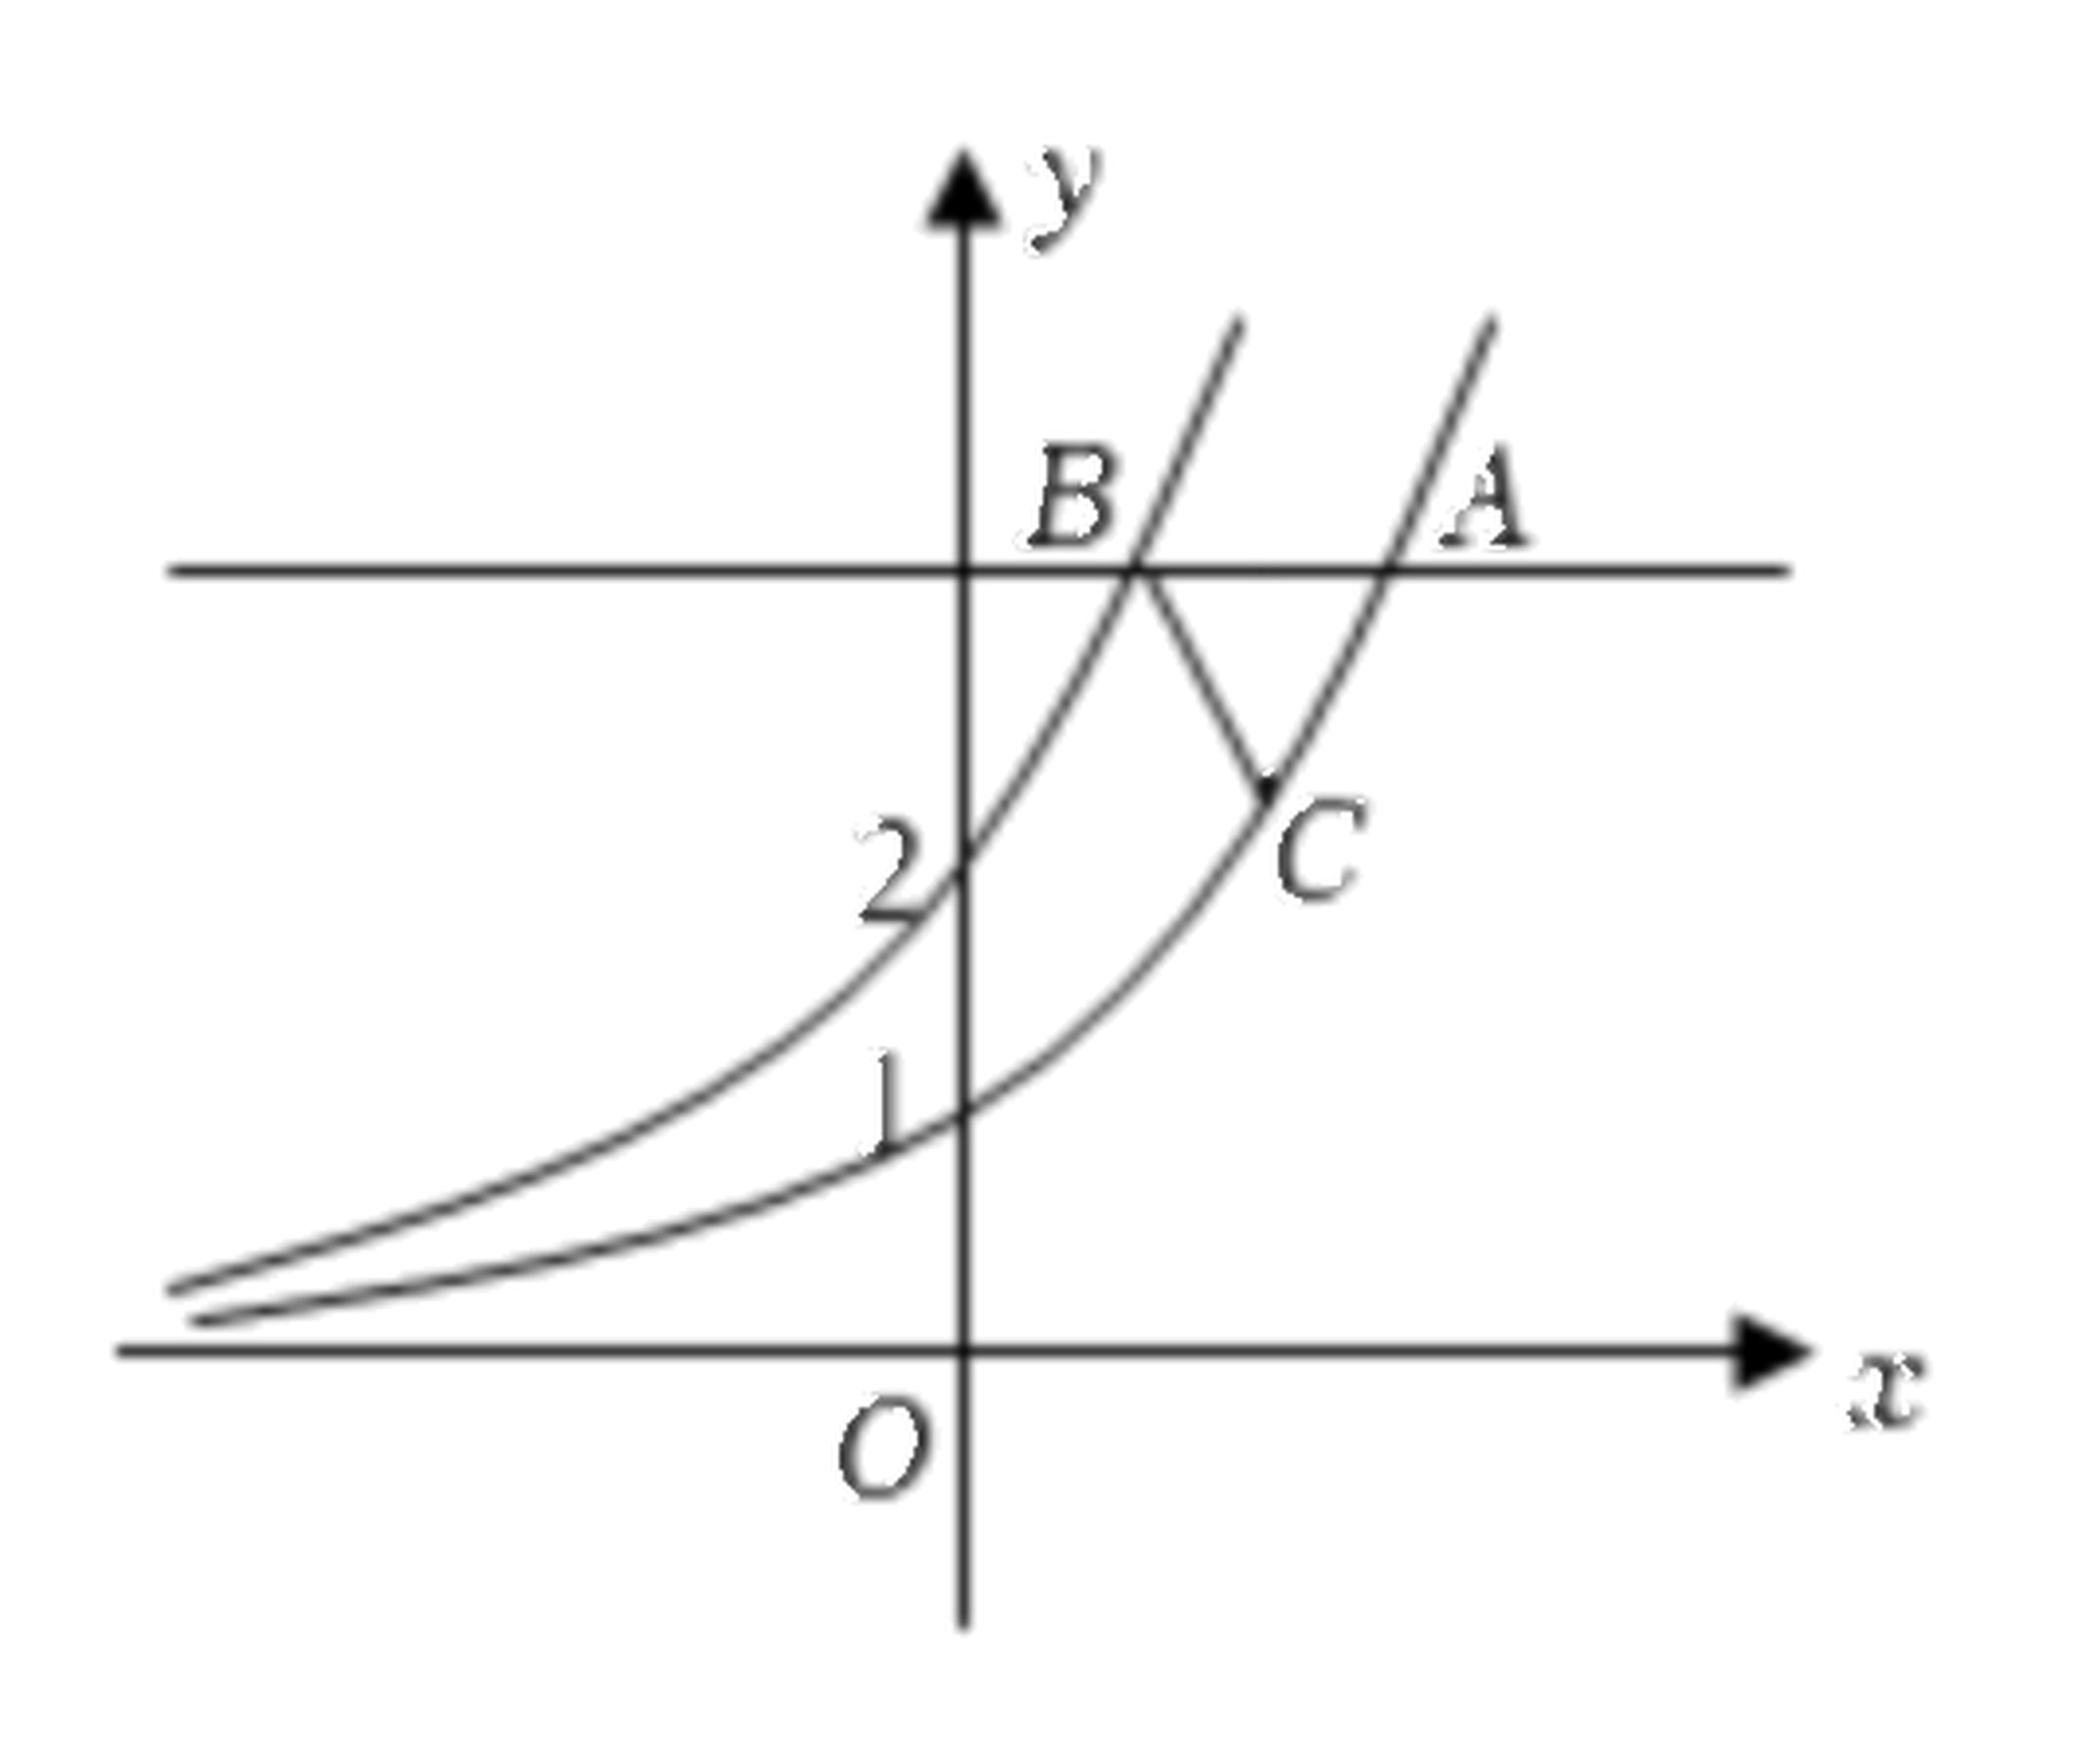
\includegraphics[width=0.40\textwidth]{figures/gao150_q11.png}
\end{center}

\ifanswer
\solbegin
\step{设直线 $l$ 的方程为 $y=a(a>0)$，}
\step{由 $2^x=a$，得 $x=\log_2 a$，所以 $A(\log_2 a,a)$，}
\step{由 $2^{x+1}=a$，得 $x=\log_2 a-1$，所以 $B(\log_2 a-1,a)$，所以 $\lvert AB\rvert=1$，}
\step{取 $AB$ 的中点 $D$，连接 $CD$，如图所示，}
\step{因为 $\triangle ABC$ 为等边三角形，则 $CD\perp AB$，且 $\lvert CD\rvert=\dfrac{\sqrt3}{2}$，}
\step{所以 $C\left(\log_2 a-\dfrac{1}{2},a-\dfrac{\sqrt3}{2}\right)$，}
\step{因为点 $C$ 在函数 $y=2^x$ 的图像上，所以 $a-\dfrac{\sqrt3}{2}=2^{\log_2 a-\frac{1}{2}}=\dfrac{a}{\sqrt2}$，}
\step{解得 $a=\dfrac{\sqrt3}{2-\sqrt2}=\dfrac{\sqrt3(2+\sqrt2)}{4-2}=\sqrt3+\dfrac{\sqrt6}{2}$，}
\step{所以点 $C$ 的纵坐标为 $a-\dfrac{\sqrt3}{2}=\dfrac{\sqrt3+\sqrt6}{2}$.}
\solend
\fi

% === Q12 === 解析配图（高斯函数方格阴影，仅答案版出）；"数学王子"弯引号；cases 块整体算一个印刷行；解析 4 行
\item 小玲在研究数学发展史，特别崇拜近代数学奠基者之一、享有“数学王子”称号的德国数学家高斯. 为了纪念高斯，我们把取整函数 $y=[x]$ 称为高斯函数，其中 $[x]$ 表示不超过 $x$ 的最大整数，如 $[1.1]=1$，$[-1.1]=-2$，则点集 $P=\{(x,y)\mid [x]^2+[y]^2=1\}$ 所表示的平面区域的面积为\blankline[4.4em].

\ifanswer
\solbegin
\step{$[x]^2+[y]^2=1$ 由 $\begin{cases}[x]=0\\ {[y]=-1}\end{cases}$ 或 $\begin{cases}[x]=0\\ {[y]=1}\end{cases}$ 或 $\begin{cases}[x]=-1\\ {[y]=0}\end{cases}$ 或 $\begin{cases}[x]=1\\ {[y]=0}\end{cases}$ 四个平面区域组成，}
\step{即 $\begin{cases}0\leqslant x<1\\ -1\leqslant y<0\end{cases}$ 或 $\begin{cases}0\leqslant x<1\\ 1\leqslant y<2\end{cases}$ 或 $\begin{cases}-1\leqslant x<0\\ 0\leqslant y<1\end{cases}$ 或 $\begin{cases}1\leqslant x<2\\ 0\leqslant y<1\end{cases}$，}
\step{作出平面区域如图所示，平面区域由四个边长为 $1$ 的正方形组成，}
\begin{center}
% 高斯函数 [x]^2+[y]^2=1 方格阴影区域图取 04 页顶部，去粉色水印、去色、4× LANCZOS 放大；仅答案版出
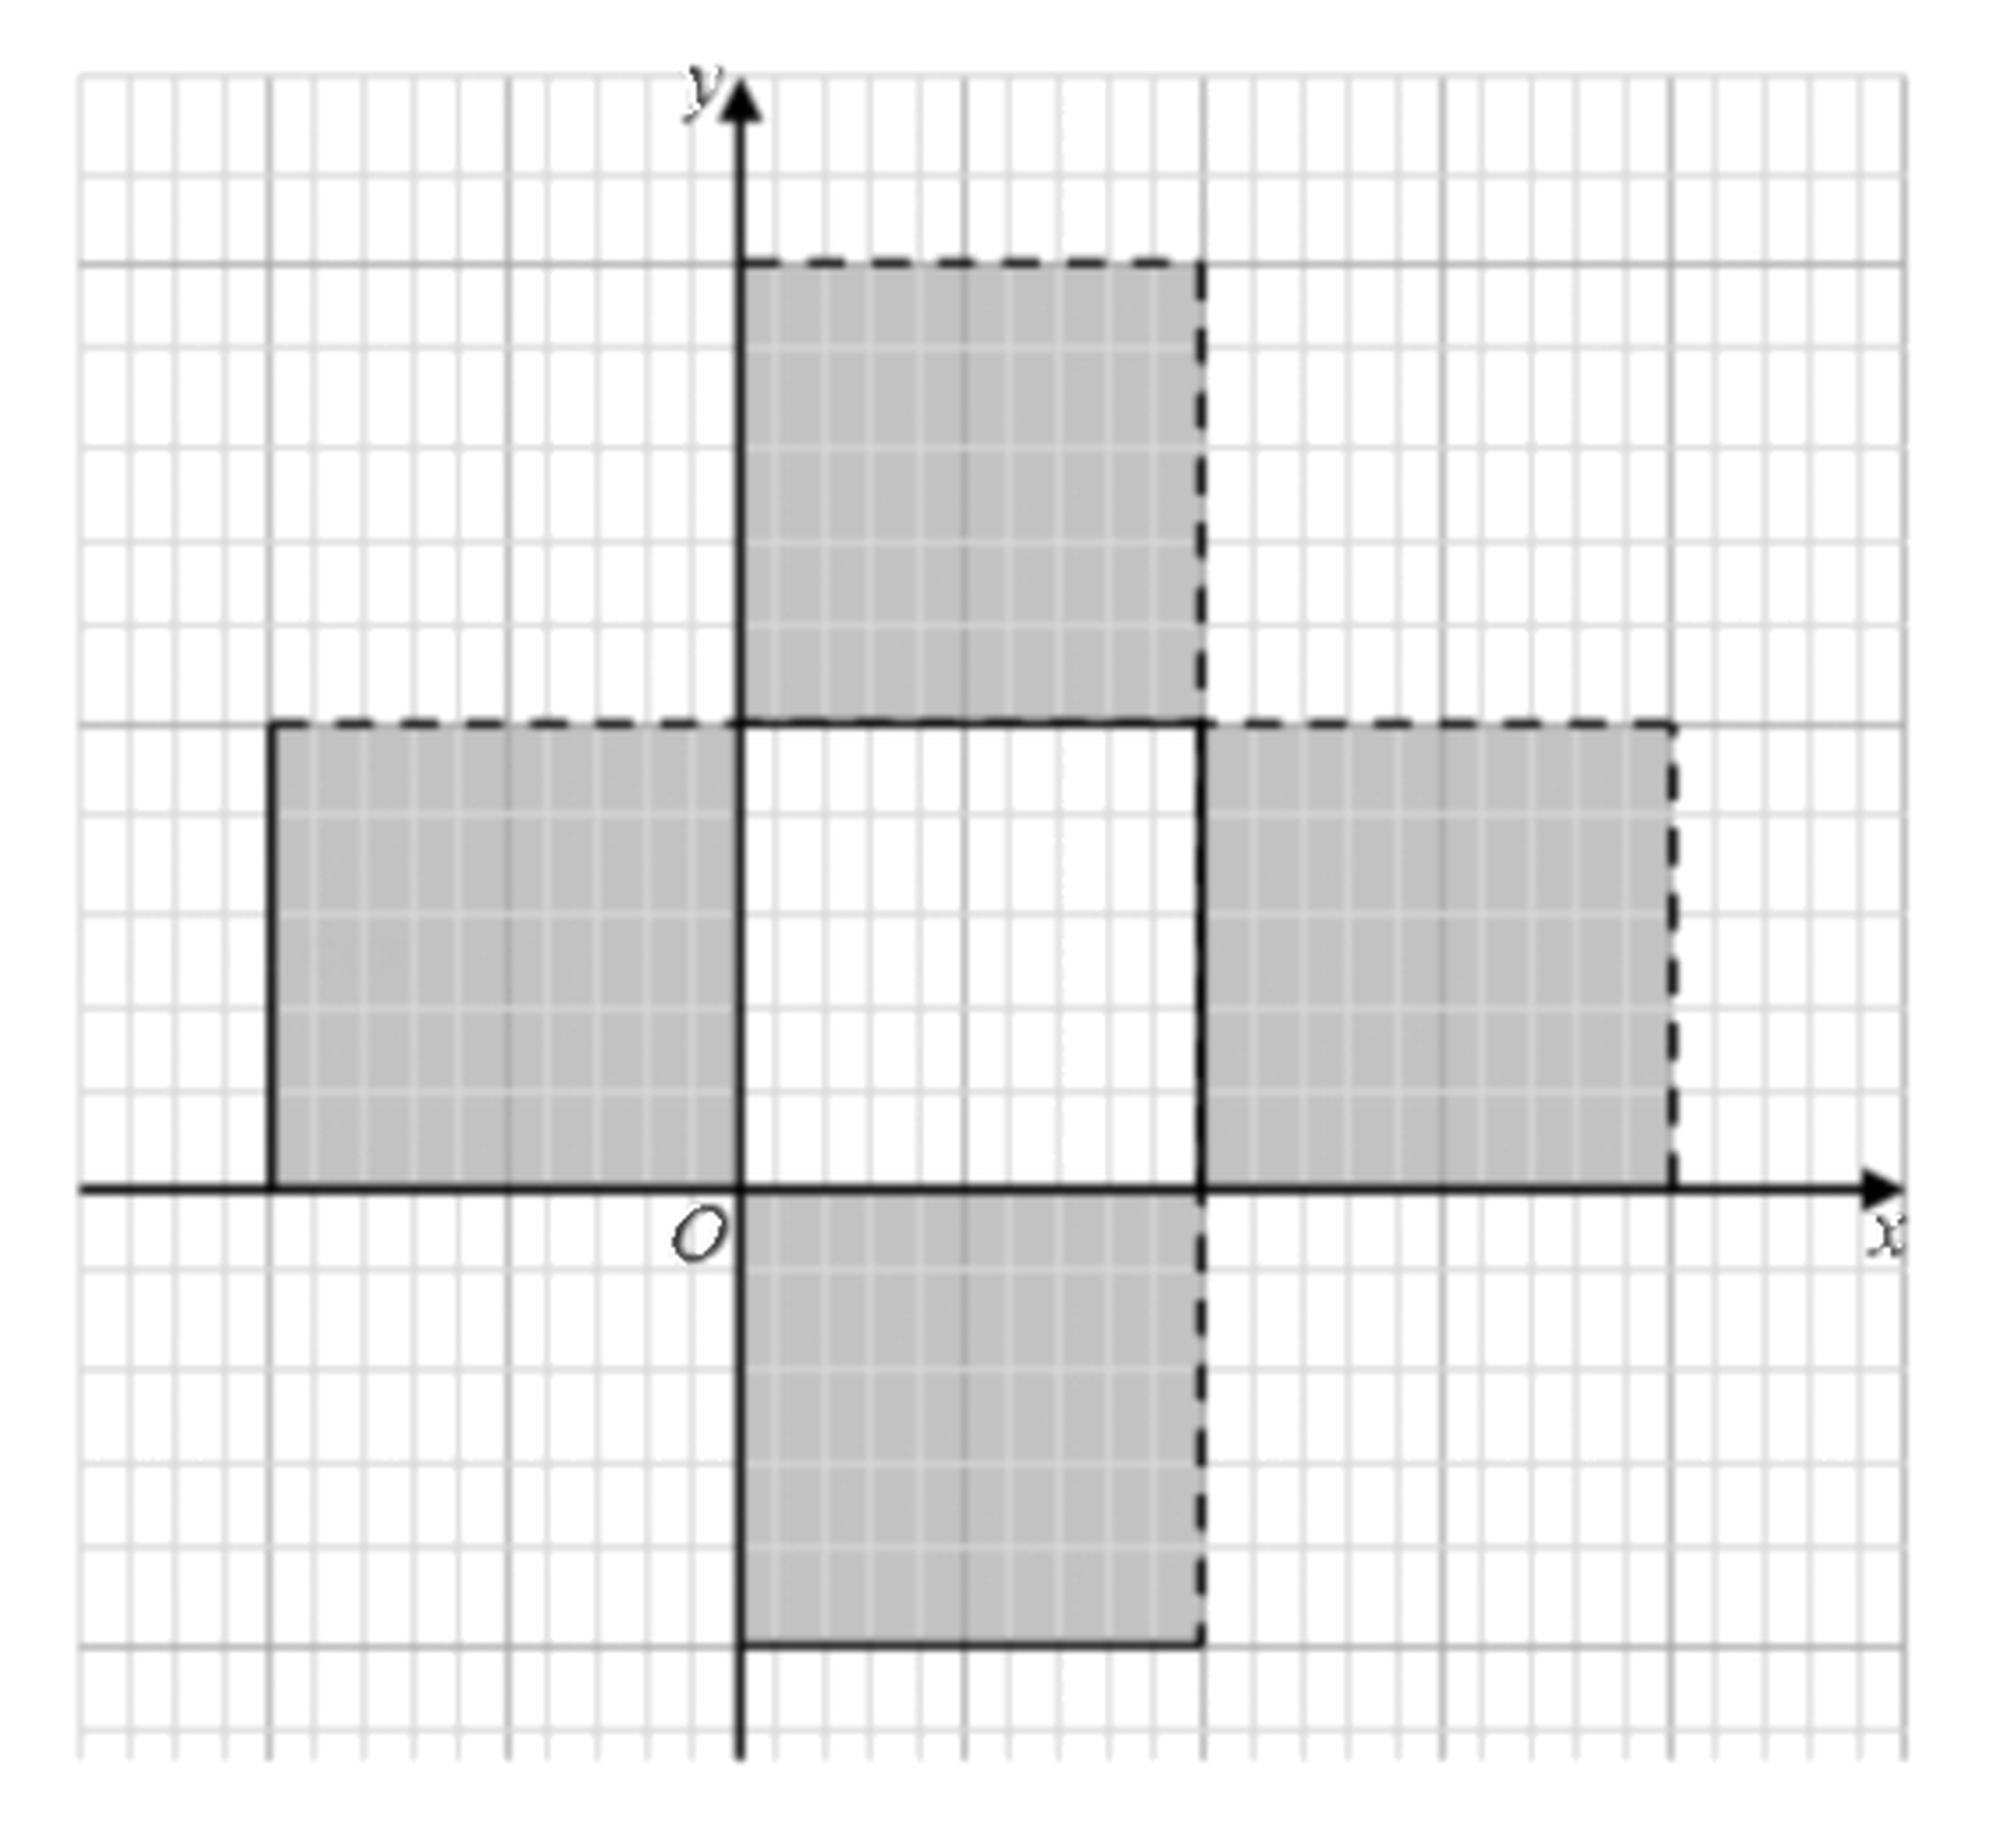
\includegraphics[width=0.34\textwidth]{figures/gao150_q12.png}
\end{center}
\step{总面积为 $1\times4=4$.}
\solend
\fi

\end{enumerate}

\bigsec{二、选择题}

\begin{enumerate}
\setcounter{enumi}{12}

% === Q13 === 答案在解析末句"故选 C"；括号 \mbox{（\quad）} 留空；四选项一行；解析 1 行
\item 设 $x\ne0$，则 $3^{\log_9 x^2}$ 的化简结果是\mbox{（\quad）}

\keepwithprev
A. $x$\qquad B. $\dfrac{1}{x}$\qquad C. $\lvert x\rvert$\qquad D. $\dfrac{1}{\lvert x\rvert}$

\ifanswer
\solbegin
\step{$3^{\log_9 x^2}=3^{\log_3\lvert x\rvert}=\lvert x\rvert$，故选 $C$.}
\solend
\fi

% === Q14 === 题目配图（两函数图像，三版都出）；\needvspace{8cm} 守卫放 \item 之前；"图像"照录；四选项两行两列；解析 2 行，故选 B
\needvspace{8cm}
\item 设 $a>0$ 且 $a\ne1$，$b\in\R$. 若函数 $y=a^{-\lvert x\rvert}$ 与 $y=x^b$ 的大致图像如图所示，则\mbox{（\quad）}

\keepwithprev
A. $0<a<1<b$\qquad\qquad B. $a>1$ 且 $b>1$

C. $0<a<1$ 且 $0<b<1$\qquad\qquad D. $0<b<1<a$

\begin{center}
% 两函数 y=a^{-|x|} 与 y=x^b 大致图像取 04 页右侧，去粉色水印、去色、4× LANCZOS 放大；三版都出
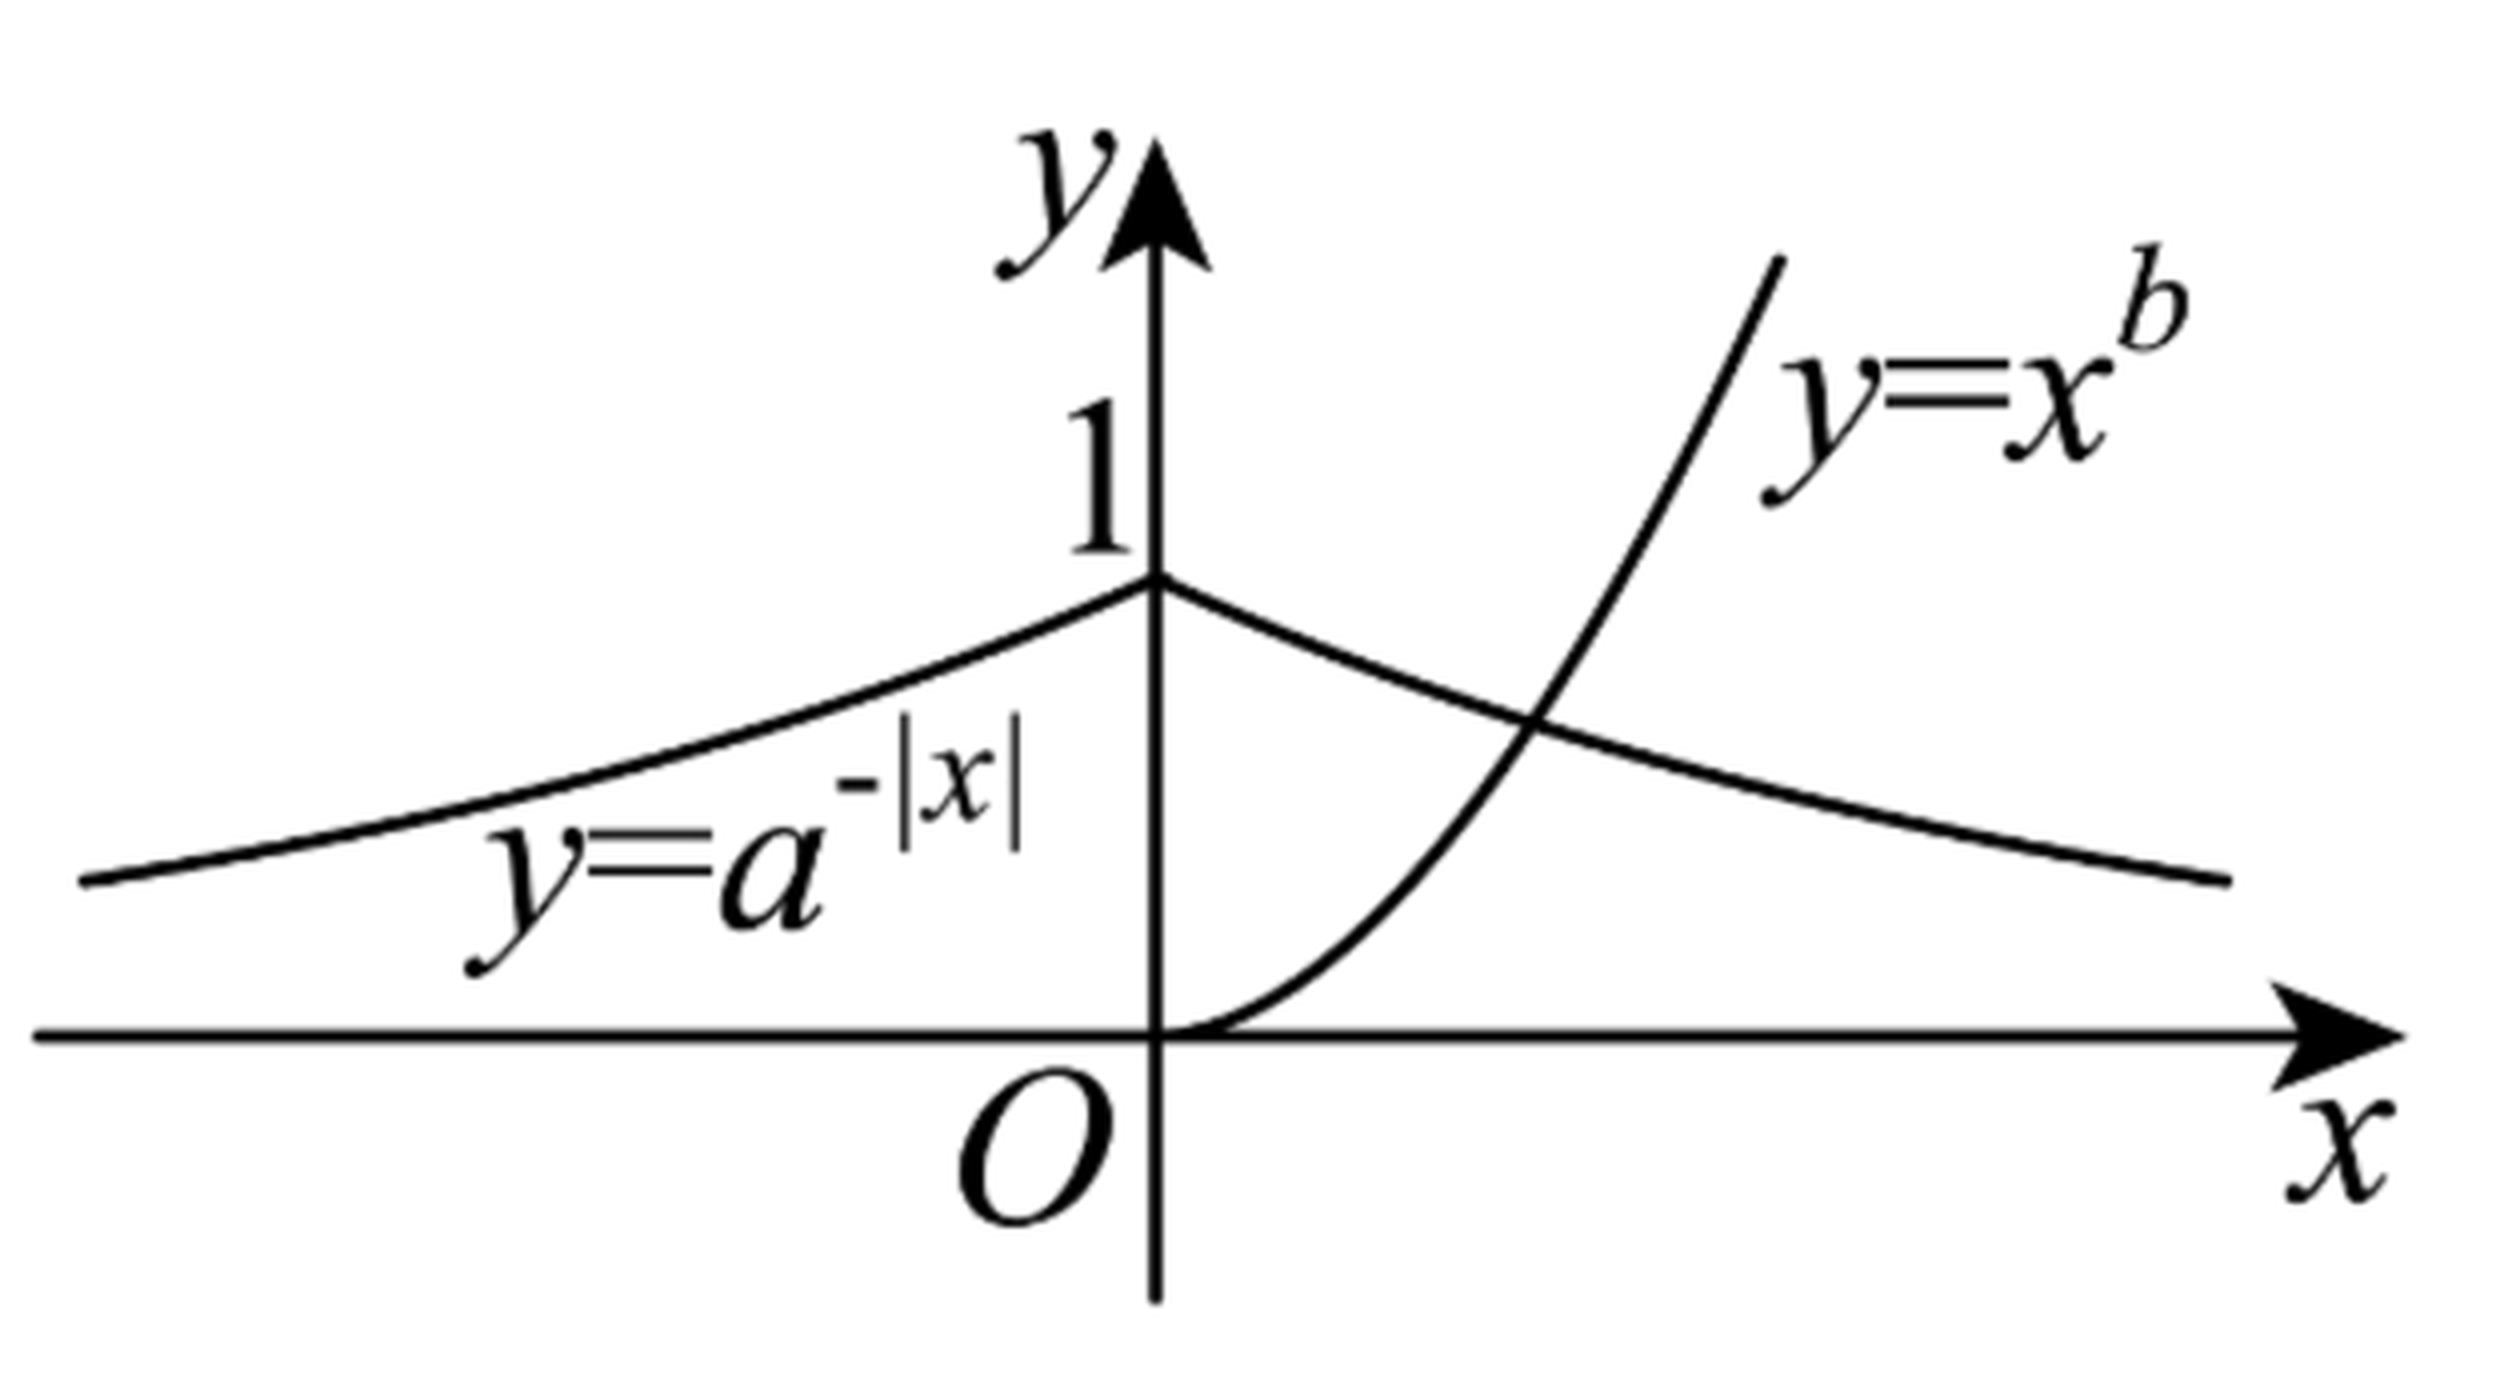
\includegraphics[width=0.40\textwidth]{figures/gao150_q14.png}
\end{center}

\ifanswer
\solbegin
\step{在 $(0,+\infty)$ 上，$y=a^{-x}$ 严格递减，得 $a>1$；}
\step{幂函数 $y=x^b$ 的图像递增且向上弯曲，得 $b>1$；故选 $B$.}
\solend
\fi

% === Q15 === "算术平均值／算术平均数"两处不同照录；四选项两行两列；解析 5 行（续 05 页顶），故选 B
\item 已知两个正数的算术平均值不小于它们的几何平均值，类比有以下结论：三个正数的算术平均数不小于它们的几何平均数，即当 $a,b,c$ 为正实数时，$\dfrac{a+b+c}{3}\geqslant\sqrt[3]{abc}$，当且仅当 $a=b=c$ 时等号成立. 利用上述结论，下列选项中判断正确的是\mbox{（\quad）}

\keepwithprev
A. 若 $x>0$，则 $2x+\dfrac{1}{x^2}\geqslant\dfrac{27}{8}$\qquad\qquad B. 若 $x>0$，则 $x^2+\dfrac{2}{x}\geqslant3$

C. 若 $0<x<1$，则 $x^2(1-x)\geqslant\dfrac{1}{9}$\qquad\qquad D. 若 $0<x<1$，则 $x^2(1-x)\leqslant\dfrac{1}{9}$

\ifanswer
\solbegin
\step{A：取 $x=1$，$2x+\dfrac{1}{x^2}=3<\dfrac{27}{8}$，错误.}
\step{B：$x^2+\dfrac{2}{x}=x^2+\dfrac{1}{x}+\dfrac{1}{x}\geqslant3\sqrt[3]{x^2\cdot\dfrac{1}{x}\cdot\dfrac{1}{x}}=3$，当且仅当 $x=1$ 时取等号，正确.}
\step{C：取 $x=\dfrac{1}{3}$，$x^2(1-x)=\dfrac{2}{27}<\dfrac{1}{9}$，错误.}
\step{D：取 $x=\dfrac{2}{3}$，$x^2(1-x)=\dfrac{4}{27}>\dfrac{1}{9}$，错误.}
\step{故选 $B$.}
\solend
\fi

% === Q16 === "完美集"新定义（弯引号、引号外空格照录）；圈数字①②文本模式；$n\in\N$；四选项两行两列；解析 9 行（6 行 05 页＋3 行 06 页顶），故选 A
\item 已知有限集 $A=\{a_1,a_2,\cdots,a_n\}$（$n\geqslant2$，$n\in\N$）. 若 $A$ 中元素 $a_i$（$i=1,2,\cdots,n$）满足 $a_1+a_2+\cdots+a_n=a_1\cdot a_2\cdots a_n$，就称 $A$ 为 “完美集”. 现有以下两个命题：

①恰有两个元素的 “完美集” 有无穷多个；

②若 $a_i$ 均为正整数，则 “完美集” $A$ 有且只有一个，且 $n=3$.

则\mbox{（\quad）}

\keepwithprev
A. ①和②都是真命题\qquad\qquad B. ①和②都是假命题

C. ①是真命题，②是假命题\qquad\qquad D. ①是假命题，②是真命题

\ifanswer
\solbegin
\step{①由 $a+b=ab\Leftrightarrow(a-1)(b-1)=1$，任取 $a>2$，则 $b=1+\dfrac{1}{a-1}\in(1,2)$，}
\step{得到无穷多个不同的完美集，①真.}
\step{②设 $1\leqslant a_1<a_2<\cdots<a_n$，则 $a_i\geqslant i$.}
\step{若 $n=2$，则 $(a_1-1)(a_2-1)=1$，只能有 $a_1=a_2=2$，与元素互异矛盾.}
\step{若 $n\geqslant4$，则 $a_1a_2\cdots a_n\geqslant a_2a_{n-1}a_n\geqslant2(n-1)a_n>na_n\geqslant a_1+\cdots+a_n$，矛盾.}
\step{当 $n=3$ 时，若 $a_1\geqslant2$，则 $a_1a_2a_3\geqslant6a_3>3a_3\geqslant a_1+a_2+a_3$，矛盾.}
\step{因此 $a_1=1$，$(a_2-1)(a_3-1)=2$，结合 $a_2<a_3$ 得 $a_2=2$，$a_3=3$.}
\step{唯一的完美集为 $\{1,2,3\}$，②真.}
\step{故选 $A$.}
\solend
\fi

\end{enumerate}

\bigsec{三、解答题}

\begin{enumerate}
\setcounter{enumi}{16}

% === Q17 === \varnothing 空集、$B\subseteq A$ 带下划线照录；弯引号内空格照录；解析 7 行
\item 设 $a,b\in\R$. 已知集合 $A=\{x\mid ax^2+3x-a>3\}$，$B=\{x\mid bx=1\}$.

(1) 若 $A=(1,2)$，求 $a$ 的值；

(2) 若 $a=0$，且 “ $x\in A$ ” 是 “ $x\in B$ ” 的必要非充分条件，求 $b$ 的取值范围.

\ifanswer
\solbegin
\step{(1) $A=(1,2)$，则 $a<0$，且 $1,2$ 是方程 $ax^2+3x-a-3=0$ 的两根.}
\step{由 $4a+6-a-3=0$，得 $a=-1$，此时不等式为 $-(x-1)(x-2)>0$，}
\step{解集确为 $(1,2)$.}
\step{(2) $a=0$ 时，$A=(1,+\infty)$，题意等价于 $B\subseteq A$ 且 $B\ne A$.}
\step{当 $b=0$ 时，$B=\varnothing$，符合条件.}
\step{当 $b\ne0$ 时，$B=\left\{\dfrac{1}{b}\right\}$，条件等价于 $\dfrac{1}{b}>1$，解得 $0<b<1$.}
\step{因此 $b$ 的取值范围为 $[0,1)$.}
\solend
\fi

% === Q18 === $p\in\Z$；"图像"（像，有亻）照录；指数 $-2p^2+5p$；解析 8 行（(1) 首行 06 页末＋2 行 07 页顶、(2) 5 行 07 页）
\item 设 $p\in\Z$，已知 $f(x)=x^{-2p^2+5p}$.

(1) 若幂函数 $y=f(x)$ 的图像关于原点成中心对称，且满足 $f(3)<f(4)$，求 $p$ 的值；

(2) 当 $p=-2$ 时，求满足 $f(2x+3)<f(x-4)$ 的 $x$ 的取值范围.

\ifanswer
\solbegin
\step{(1) 图像关于原点成中心对称，得整数 $-2p^2+5p$ 为奇数.}
\step{由 $f(3)<f(4)$，得 $-2p^2+5p>0\Leftrightarrow0<p<\dfrac{5}{2}$，}
\step{结合 $p\in\Z$，得 $p=1$ 或 $p=2$，对应指数分别为 $3$、$2$，所以 $p=1$.}
\step{(2) 当 $p=-2$ 时，$f(x)=\dfrac{1}{x^{18}}$，定义域为 $\{x\in\R\mid x\ne0\}$.}
\step{原不等式要求 $x\ne-\dfrac{3}{2}$ 且 $x\ne4$，}
\step{此时 $\dfrac{1}{(2x+3)^{18}}<\dfrac{1}{(x-4)^{18}}\Leftrightarrow\lvert 2x+3\rvert>\lvert x-4\rvert\Leftrightarrow(2x+3)^2>(x-4)^2$，}
\step{因此 $(x+7)(3x-1)>0\Leftrightarrow x<-7$ 或 $x>\dfrac{1}{3}$，}
\step{排除 $x=4$，得 $x\in(-\infty,-7)\cup\left(\dfrac{1}{3},4\right)\cup(4,+\infty)$.}
\solend
\fi

% === Q19 === $a\in\R$、$g(x)=f(2x+1)+a\cdot f(x)+2$；解析 6 行（(2) 末两行续 08 页顶）
\item 已知 $f(x)=2^x$.

(1) 求方程 $f(2x)-f(x)=6$ 的解；

(2) 设 $a\in\R$，$g(x)=f(2x+1)+a\cdot f(x)+2$，若对于任意 $x\in[-1,1]$，均有 $g(x)\geqslant1$，求 $a$ 的取值范围.

\ifanswer
\solbegin
\step{(1) 令 $t=2^x>0$，则 $t^2-t-6=(t-3)(t+2)=0$，}
\step{由 $t>0$ 得 $t=3$，所以 $x=\log_2 3$.}
\step{(2) 令 $t=2^x$，则 $t\in\left[\dfrac{1}{2},2\right]$，且 $g(x)\geqslant1\Leftrightarrow2t^2+at+1\geqslant0\Leftrightarrow a\geqslant-\left(2t+\dfrac{1}{t}\right)$，}
\step{由基本不等式得 $2t+\dfrac{1}{t}\geqslant2\sqrt{2t\cdot\dfrac{1}{t}}=2\sqrt2$，}
\step{当且仅当 $t=\dfrac{1}{\sqrt2}\in\left[\dfrac{1}{2},2\right]$ 时等号成立，}
\step{因此 $-\left(2t+\dfrac{1}{t}\right)$ 的最大值为 $-2\sqrt2$，所求范围为 $a\in[-2\sqrt2,+\infty)$.}
\solend
\fi

% === Q20 === "极闭集"新定义、3 问，全卷末题；$M\subseteq(0,+\infty)$ 带下划线照录；自定义运算 $x*y$ 星号照录；解析 13 行（9 行 08 页＋4 行 09 页上半）
\item 对于非空实数集 $M\subseteq(0,+\infty)$，若满足以下两个条件：

① $M$ 中至少含有 $2$ 个元素，且 $1\notin M$；

②对于 $M$ 中任意两个不相等的元素 $x$、$y$，定义 $x*y=\dfrac{xy+1}{x+y}$，且 $x*y\in M$.

则称 $M$ 为 “极闭集”.

(1) 分别判断集合 $A=\left\{\dfrac{1}{2},3\right\}$ 与集合 $B=(1,+\infty)$ 是否为 “极闭集” （无需理由）；

(2) 若 $M$ 是 “极闭集”，证明：$M$ 中不可能所有元素都小于 $1$；

(3) 证明：不存在任何有限集是 “极闭集”.

\ifanswer
\solbegin
\step{(1) $A$ 不是 “极闭集”，$B$ 是 “极闭集”.}
\step{(2) 假设 $M$ 中所有元素都小于 $1$，取其中两个不相等的元素 $x$、$y$，}
\step{则 $x*y-1=\dfrac{(1-x)(1-y)}{x+y}>0$，}
\step{这与 $x*y\in M$ 且 $M$ 中所有元素都小于 $1$ 矛盾.}
\step{(3) 假设有限集 $M$ 是 “极闭集”，}
\step{由 (2) 及 $1\notin M$，得 $M$ 中存在大于 $1$ 的元素.}
\step{若 $M$ 中有小于 $1$ 的元素，取其中最大的一个为 $a$，另取 $b\in M$ 且 $b>1$，}
\step{则 $a*b-a=\dfrac{1-a^2}{a+b}>0, a*b-1=\dfrac{(a-1)(b-1)}{a+b}<0$，}% 半角逗号在两个数学式组之间，全稿惯例、非笔误，照录
\step{于是 $a<a*b<1$ 且 $a*b\in M$，与 $a$ 的最大性矛盾.}
\step{若 $M$ 中没有小于 $1$ 的元素，则 $M\subseteq(1,+\infty)$.}
\step{取 $a=\min M$，另取 $b\in M$ 且 $b\ne a$，则 $a*b-a=\dfrac{1-a^2}{a+b}<0$，}
\step{于是 $a*b<a$ 且 $a*b\in M$，与 $a$ 的最小性矛盾.}
\step{因此不存在任何有限集是 “极闭集”.}
\solend
\fi

\end{enumerate}

\end{document}
"
% 紧凑版：xelatex "\def\iscompact{1}% 高一150_曹杨二中_期中.tex
%   —— 高一上数学"2026-2027 年曹杨二中高一上期中"（试卷版/答案版/紧凑版）
% 试卷版：xelatex 高一150_曹杨二中_期中.tex
% 答案版：xelatex "\def\isanswer{1}% 高一150_曹杨二中_期中.tex
%   —— 高一上数学"2026-2027 年曹杨二中高一上期中"（试卷版/答案版/紧凑版）
% 试卷版：xelatex 高一150_曹杨二中_期中.tex
% 答案版：xelatex "\def\isanswer{1}% 高一150_曹杨二中_期中.tex
%   —— 高一上数学"2026-2027 年曹杨二中高一上期中"（试卷版/答案版/紧凑版）
% 试卷版：xelatex 高一150_曹杨二中_期中.tex
% 答案版：xelatex "\def\isanswer{1}\input{高一150_曹杨二中_期中.tex}"
% 紧凑版：xelatex "\def\iscompact{1}\input{高一150_曹杨二中_期中.tex}"
%
% ① 原始材料：微信公众号"魔都数学加油站"文章，连载"27学年高一150"，原文标题
% "27学年高一150——2026-2027年上海市曹杨二中高一上期中"；
% 原文链接：https://mp.weixin.qq.com/s/xlQxmik8TZXR87RC6MnCrw 。
% 正文为 9 张 PNG 页（01/02/04/06/07/09 为 2560×3620，03/05/08 为 4762×6735，
% 同一篇各页分辨率混排，逐页按各自分辨率裁图核对，别按预览比例换算裁框）。
% 体例：讲评版——全 18 题均印【解析】（逐题核实，见 ② ②）。
% 题目、答案、解析均据原图转录；卷面粉红色/红色水印"魔都数学加油站"及公众号页脚未录入。
% 全卷插图清单（逐页通读 9 页确认）：3 幅——
%   · Q11 题目配图（指数函数曲线图，02 页右侧：x/y 轴、O、y=2^x 与 y=2^{x+1}
%     两曲线、A/B/C 三点、刻度 1/2、等边三角形 ABC），三版都出，裁 figures/gao150_q11.png；
%   · Q12 解析配图（高斯函数取整 [x]^2+[y]^2=1 方格阴影区域图，04 页顶部：4 个边长 1
%     的正方形组成的十字形阴影），解析"作出平面区域如图所示"处，仅答案版出，
%     放 \ifanswer 内 \step 之间，裁 figures/gao150_q12.png；
%   · Q14 题目配图（两函数 y=a^{-|x|} 与 y=x^b 大致图像，04 页右侧：x/y 轴、O、
%     y 轴刻度 1、一递减曲线一递增上翘曲线），三版都出，裁 figures/gao150_q14.png；
%   其余各页逐页确认无其它题目配图、无表格；Q11/Q12 解析"如图所示"对应的就是上列
%   已裁的图，不重复裁；09 页上半为 Q20(3) 解析续尾、下半仅水印、无正文。
%   3 图均取自原卷截图，去粉色水印、去色、4× LANCZOS 放大。
%
% 卷首标题：原卷印作"2026-2027 年曹杨二中高一上期中"，年份区间按全稿惯例排 en dash；
% 原卷卷面未印副标题，本稿按同期中卷知识模块口径补出"集合与常用逻辑用语、不等式、函数"。
%
% 题号体例（逐页核实定稿）：本卷共 18 题——一、填空题 3—12（10 题）、
% 二、选择题 13—16（4 题）、三、解答题 17—20（4 题）。
% 三节分别 \setcounter{enumi}{2}／{12}／{16}。原卷从第 3 题起、无第 1、2 题，
% 本稿保留原题号；全卷末题为第 20 题（"极闭集"新定义、3 问），无 Q21、无附加题节。
%
% ② 与原卷的排版差异：
%   ① 原文从第 3 题起，本稿保留原题号；共 18 题三节，解答题只有 4 题到 20；
%   ② 全 18 题均印【解析】，用 \solbegin…\solend；逐题核实无只印【答案】或
%      答案印题干括号内的题；四道选择题答案在解析末句"故选 X"（Q13 选 C、
%      Q14 选 B、Q15 选 B、Q16 选 A，逐个放大复核）、括号 \mbox{（\quad）} 留空、
%      不另提 \ans{}；答案版【答案】/【解析】标记数 = 18 = 全卷题数；
%   ③ 原卷卷面未印副标题，本稿按知识模块口径补出；
%   ④ 原卷填空横线按全稿惯例排 \blankline[4.4em]；选择题括号排 \mbox{（\quad）}、
%      选项段前按惯例加 \keepwithprev；解答题不留作答区、不加 \anspace（原卷为讲评版）；
%   ⑤ 数集黑板粗体：Q4"m\in R"、Q5"a,b\in R"、Q6"a,b,c\in R"、Q7"a\in R"、
%      Q10"a\in R"、Q14"b\in R"、Q17"a,b\in R"、Q18"p\in Z"／定义域"x\in R"、
%      Q19"a\in R"、Q16"n\in N" 原卷印斜体 R/Z/N，按全稿惯例归一 \R／\Z／\N；
%      绝对值排 \lvert…\rvert（Q7 |x+4|+|x-3|、Q11 |AB|／|CD|、Q13 |x|、
%      Q18 |2x+3|／|x-4|），集合描述竖线排 \mid（Q3、Q12、Q17、Q18、Q20），
%      不等号按全稿惯例排 \leqslant／\geqslant；补集照原卷上划线排 \overline{A}
%      （Q3 题干＋解析共 2 处）；空集符号 \varnothing（Q17 解析(2)）；
%      子集 \subset（单线⊂）／\subseteq（带下划线⊆）逐处照录，本卷 3 处子集
%      符号均印带下划线 ⊆、照录 \subseteq（Q20 题干、Q20 解析(3)、Q17 解析(2)，
%      见 ④），无 \subset 用例；
%   ⑥ 判别式 Δ/△：逐页通读 9 页，本卷无一元二次判别式算式，故无 Δ/△ 混用可照录
%      （"高 \Delta／扁 \triangle"口径备查，参照 高一142／144／145／146／148／149
%      头注④）；本卷仅 Q11 题干与解析共 2 处几何三角形符号 △ABC，逐处放大并排
%      确认两处同形、印近等边粗线三角（非判别式），照录 \triangle（见 ④）；
%   ⑦ 中文弯引号照录：Q12"数学王子"、Q16"完美集"（题干＋①②两命题，引号外
%      留空格）、Q17" x∈A "" x∈B "（引号内空格）、Q20"极闭集"（题干条件、
%      三问与解析，引号外留空格）；注释里一律 ASCII 引号；数学式内 CJK 用 \text{}
%      （Q3 集合描述"且"用 \text{ 且 }）；
%   ⑧ 半角逗号在数学组之间是全稿惯例、非笔误，逐处照录（Q17 解析"1,2 是方程…
%      两根"、Q20 解析(3)">0, a*b-1=…<0" 两式之间等）；行末西文句点 ASCII `.`；
%      行中全角逗号／顿号照录（Q12"之一、享有"、Q18 解析"3、2"、Q20"x、y"）；
%   ⑨ "图像／图象"逐处放大核：全卷 9 处均印"图像"（像，有亻）、未见"图象"——
%      Q4 题干 1、Q11 题干 2＋解析 1、Q14 题干 1＋解析 1、Q18 题干 1＋解析 1；
%      同卷"第二象限""象限"用"象"（无亻）。逐处照录未统一改动（放大 01/02/04/06
%      页 /tmp/gao150/z/p01_q4_tuxiang2.png、p04_q14_tuxiang2.png、
%      p02_q11_lines.png 确认）；子题标号 (1)(2)(3) 半角括号照录；圈数字①②
%      在文本模式（Q16 两命题与解析、Q20 两条件与三问及解析）按 common.sty
%      划入 CJK 字符类渲染，进数学式用 \text{①}；
%   ⑩ Q20 新定义 x*y=\dfrac{xy+1}{x+y} 的 * 是自定义运算（星号），照录；
%      \left…\right 不得拆到不同 $…$ 组（Q19"\left(2t+\frac1t\right)"、
%      Q20 题干"A=\left\{\frac12,3\right\}"等）；Q8 嵌套根号
%      \sqrt{\frac2x+\frac{16}{1-2x}}、Q9 对数连加 \log_2 A 等复杂式照录别简化；
%   ⑪ 一条 \step = 原卷解析的一个印刷行，cases 块整体算一个印刷行；别并折行、
%      别拆行。Q4 三行、Q8 五行、Q11 九行、Q12 四行（两行各含四个 cases 块）、
%      Q15 五行、Q16 九行、Q18 八行、Q20 十三行均按印刷行逐条断，不丢行；
%   ⑫ 配图：Q11／Q14 题目配图（三版都出）放 \item 内题干之后 \begin{center}，
%      大图块加 \needvspace{8cm} 守卫把整块推走（守卫放 \item 之前，见
%      高一145 Q14/Q20 成例与切页审计 B 类坑）；Q12 解析配图（仅答案版出）
%      放 \ifanswer 内 \solbegin…\solend 的 \step 之间（高一73 第16题成例）；
%   ⑬ 跨页续印按题合并：见 ⑥；
%   ⑭ 原卷解析内无红色"法一／法二"之类小标题，故本卷无 \stepm；红色水印
%      "魔都数学加油站"不录入；Q12 解析"作出平面区域如图所示"对应的图即
%      ① 所列 gao150_q12.png（04 页顶部），不重复裁；Q11 解析"如图所示"对应
%      题目配图 gao150_q11.png，不另裁。
%
% ③ 行数复核：一条 \step／\stepm = 原卷解析的一个印刷行，cases 块作一个印刷行计。
%   逐题数（主会话逐页核对定稿）：Q3：1；Q4：3；Q5：2；Q6：1；Q7：2；Q8：5；
%   Q9：1；Q10：3；Q11：9；Q12：4；Q13：1；Q14：2；Q15：5；Q16：9；
%   Q17：7；Q18：8；Q19：6；Q20：13。
%   合计 82 条 \step（本卷无 \stepm：解析内无红色"法一／法二"类小标题），
%   与原卷逐题印刷行相等。全卷 18 题均设 \solbegin…\solend，答案版
%   【答案】/【解析】标记数 = 18 = 全卷题数。
%
% ④ 判别式／三角形／子集符号结论（逐处放大原图照录、不得统一，主会话像素级复核）：
%   判别式：逐页通读 9 页，本卷无一元二次判别式 Δ/△ 算式（Q18 讨论幂函数指数
%     奇偶、不用判别式；Q9／Q19／Q20 亦无），头注 ② ⑥ 的"高 \Delta／扁 \triangle"
%     口径在本卷无对应处（参照 高一142／144／145／146／148／149 头注④，仅备查）。
%   几何三角形符号：Q11 题干"使得 △ABC 为等边三角形"（02 页末）与解析
%     "因为 △ABC 为等边三角形，则 CD⊥AB"（03 页）共 2 处，放大 02/03 页
%     /tmp/gao150/z/q11_tri_montage2.png 并排确认两处同形、印近等边粗线三角
%     （h/w≈0.98、非"高>宽"的判别式 \Delta），照录 \triangle（与 高一105
%     "使得 \triangle ABC 为等边三角形" 同短语成例、高一149 几何三角形照录
%     \triangle 口径一致），不引入 \Delta。
%   子集／补集：Q20 题干"$M\subseteq(0,+\infty)$"（08 页）、Q20 解析(3)
%     "则 $M\subseteq(1,+\infty)$"（09 页）、Q17 解析(2)"题意等价于 $B\subseteq A$
%     且 $B\ne A$"（06 页）共 3 处子集符号，逐处放大（/tmp/gao150/z/p08_q20_stem.png、
%     p09_q20_sub.png、p06_q17_sub.png）确认均印带下划线 ⊆，照录 \subseteq；
%     本卷未见单线 ⊂（\subset）之对应处。Q3 题干与解析共 2 处补集照原卷上划线
%     排 \overline{A}；Q17 解析(2) 空集印 ∅、照录 \varnothing（Q7"解集为空集"
%     为中文词、非符号，照录文字）；集合描述竖线 \mid；数集 \R／\Z／\N 归一见 ② ⑤。
%
% ⑤ 存疑照录（放大原图确认，照录未改、正文对应处另有 % 注）：
%   1. Q8 解析第 4 行"所以 $y=\frac1x+\frac{8}{1-2x}$ 的最小值为 18" —— 上文
%      并未定义 $y$，且题面求的是 $\sqrt{\frac2x+\frac{16}{1-2x}}$ 的最小值；
%      按上下文该行应为 $\frac1x+\frac{8}{1-2x}$ 的最小值为 18（$y$ 疑为原卷
%      衍字／笔误），放大 02 页 /tmp/gao150/z/p02_q8_y.png 确认，照录未改。
%   2. Q20 解析(3)"$a*b-a=\frac{1-a^2}{a+b}>0, a*b-1=\frac{(a-1)(b-1)}{a+b}<0$"
%      两式之间的逗号原卷印半角 ,（非全角），按全稿惯例"半角逗号在数学组之间"
%      照录未改（放大 08 页 /tmp/gao150/z/p08_q20_sol8.png 确认）。
%   3. Q15 题干"两个正数的算术平均值…几何平均值"与"三个正数的算术平均数…
%      几何平均数"两处"值／数"用字不同，逐处照录未统一（放大 04 页确认）。
%   4. "图像／图象"全卷 9 处均印"图像"（像，有亻）、未见"图象"，逐处放大核实
%      照录、未统一改动（见 ② ⑨）；本卷判别式 Δ/△ 无用例、几何三角形 2 处
%      照录 \triangle（见 ④）。
%   全卷除此 4 类外未发现其它笔误／自相矛盾处；18 题均印【解析】、无只印【答案】
%   或答案印题干括号内的题（见 ② ②）。
%
% ⑥ 跨页续印按题合并说明（逐页核实定稿）：Q3/4/5/6/7 题干＋解析在 01 页；
%   Q8 题干＋解析 5 行、Q9 题干＋解析 1 行在 02 页上半；Q10 题干＋解析 3 行
%   在 02 页下半；Q11 题干（前两行）＋配图在 02 页下半、题干续"三角形，则点 C
%   的纵坐标为___"与解析 9 行全在 03 页上半（解析"如图所示"对应题目配图）；
%   Q12 题干＋解析 4 行在 03 页下半，解析配图（方格阴影）续印在 04 页顶部；
%   "二、选择题"标题在 04 页中部；Q13 题干＋选项＋解析、Q14 题干＋选项＋
%   配图＋解析在 04 页；Q15 题干＋四选项在 04 页末、解析 5 行续 05 页上半；
%   Q16 题干＋①②两命题＋"则(  )"＋四选项＋解析前 6 行在 05 页、解析末 3 行
%   （"因此 a_1=1…②真""故选 A"）续 06 页顶部；"三、解答题"标题在 06 页；
%   Q17 题干(1)(2)＋解析(1) 3 行＋解析(2) 首行在 06 页、解析(2) 续 3 行
%   在 06 页下半；Q18 题干(1)(2)＋解析(1) 首行在 06 页末、解析(1) 续 2 行＋
%   解析(2) 5 行在 07 页上半；Q19 题干(1)(2)＋解析(1) 2 行＋解析(2) 前 2 行
%   在 07 页下半、解析(2) 末 2 行续 08 页顶部；Q20 题干（新定义＋①②两条件）
%   ＋三问＋解析(1)(2)(3) 前 9 行在 08 页、解析(3) 末 4 行续 09 页上半，
%   末行"因此不存在任何有限集是极闭集"为全卷收尾（09 页下半仅水印、无正文）。
%   本稿按题连排，不丢行、不并折行；全卷末题为第 20 题，无 Q21、无附加题节。
%
\documentclass[a4paper,11pt]{article}
\usepackage{common}

\begin{document}

\examtitlest[3]{2026--2027 年曹杨二中高一上期中}{集合与常用逻辑用语、不等式、函数}

\bigsec{一、填空题}

\begin{enumerate}
\setcounter{enumi}{2}

% === Q3 === 补集上划线 \overline{A}（题干＋解析各 1 处）；集合描述竖线 \mid、数学式内"且"用 \text{}；解析 1 行
\item 设全集 $U=\{1,2,3,4,5\}$，集合 $A=\{x\mid x^2-3x\leqslant0\text{ 且 }x\in U\}$，则 $\overline{A}=$\blankline[4.4em].

\ifanswer
\solbegin
\step{$x^2-3x\leqslant0\Leftrightarrow0\leqslant x\leqslant3$，所以 $A=\{1,2,3\}$，$\overline{A}=\{4,5\}$.}
\solend
\fi

% === Q4 === "图像"（像，有亻）逐处照录、同句"第二象限"用"象"（无亻）；解析 3 行
\item 设 $m\in\R$. 若幂函数 $y=(m^2-5m+1)x^{m+1}$ 的图像经过第二象限，则 $m=$\blankline[4.4em].

\ifanswer
\solbegin
\step{幂函数的系数为 1，故 $m^2-5m+1=1\Rightarrow m=0$ 或 $m=5$.}
\step{$m=0$ 时，$y=x$ 不经过第二象限；}
\step{$m=5$ 时，$y=x^6$ 经过第二象限，因此 $m=5$.}
\solend
\fi

% === Q5 === 解析 2 行
\item 设 $a,b\in\R$. 若 $a^2+\dfrac{b^2}{4}=1$，则 $ab$ 的最大值为\blankline[4.4em].

\ifanswer
\solbegin
\step{$1-ab=\left(a-\dfrac{b}{2}\right)^2\geqslant0$，即 $ab\leqslant1$；}
\step{当 $a=\dfrac{\sqrt2}{2}$，$b=\sqrt2$ 时取等号，最大值为 1.}
\solend
\fi

% === Q6 === 解析 1 行
\item 设 $a,b,c\in\R$. 若等式 $2x^2-3x-2=a(x-1)^2+b(x-1)+c$ 恒成立，则 $a-b+c=$\blankline[4.4em].

\ifanswer
\solbegin
\step{令 $x=0$，得 $a-b+c=-2$.}
\solend
\fi

% === Q7 === 绝对值 \lvert…\rvert；解析 2 行
\item 设 $a\in\R$. 若关于 $x$ 的不等式 $\lvert x+4\rvert+\lvert x-3\rvert<a$ 的解集为空集，则 $a$ 的取值范围是\blankline[4.4em].

\ifanswer
\solbegin
\step{$\lvert x+4\rvert+\lvert x-3\rvert\geqslant\lvert(x+4)-(x-3)\rvert=7$，当 $-4\leqslant x\leqslant3$ 时取等号.}
\step{原不等式的解集为空集当且仅当 $a\leqslant7$，即 $a\in(-\infty,7]$.}
\solend
\fi

% === Q8 === 嵌套根号 \sqrt{\frac{2}{x}+\frac{16}{1-2x}} 照录别简化；解析 5 行
\item 设 $x\in\left(0,\dfrac{1}{2}\right)$，则 $\sqrt{\dfrac{2}{x}+\dfrac{16}{1-2x}}$ 的最小值为\blankline[4.4em].

\ifanswer
\solbegin
\step{因为 $x\in\left(0,\dfrac{1}{2}\right)$，所以 $1-2x>0$，又 $2x+1-2x=1$，}
\step{所以 $\left(\dfrac{1}{x}+\dfrac{8}{1-2x}\right)(2x+1-2x)=10+\dfrac{1-2x}{x}+\dfrac{16x}{1-2x}$}
\step{$\geqslant10+2\sqrt{\dfrac{1-2x}{x}\cdot\dfrac{16x}{1-2x}}=18$，}
\step{当且仅当 $\dfrac{1-2x}{x}=\dfrac{16x}{1-2x}$ 即 $x=\dfrac{1}{6}$ 时取等号，所以 $y=\dfrac{1}{x}+\dfrac{8}{1-2x}$ 的最小值为 18，}% 原卷此处径写 $y=\frac1x+\frac{8}{1-2x}$（上文未定义 $y$、且与题面根式不符），疑笔误，放大 02 页确认，照录未改（见 ⑤）
\step{所以 $\sqrt{\dfrac{2}{x}+\dfrac{16}{1-2x}}$ 的最小值为 6.}
\solend
\fi

% === Q9 === 对数连加 \log_2 A 等复杂式照录别简化；解析 1 行
\item 记 $A=1\times2\times3\times\cdots\times2026$，则 $\dfrac{1}{\log_2 A}+\dfrac{1}{\log_3 A}+\dfrac{1}{\log_4 A}+\cdots+\dfrac{1}{\log_{2026}A}=$\blankline[4.4em].

\ifanswer
\solbegin
\step{原式 $=\log_A 2+\cdots+\log_A 2026=\log_A(2\times3\times\cdots\times2026)=\log_A A=1$.}
\solend
\fi

% === Q10 === "严格减函数／不恒为负／⇔"照录；解析 3 行
\item 设 $a\in\R$，$f(x)=\dfrac{ax+1}{x+2}$. 若函数 $y=f(x)$ 在 $[1,+\infty)$ 上是严格减函数，且在 $[1,+\infty)$ 上的函数值不恒为负，则 $a$ 的取值范围是\blankline[4.4em].

\ifanswer
\solbegin
\step{当 $1\leqslant x_1<x_2$ 时，$f(x_2)-f(x_1)=\dfrac{(2a-1)(x_2-x_1)}{(x_1+2)(x_2+2)}$，故严格递减 $\Leftrightarrow a<\dfrac{1}{2}$.}
\step{此时最大函数值为 $f(1)$，函数值不恒为负 $\Leftrightarrow f(1)=\dfrac{a+1}{3}\geqslant0\Leftrightarrow a\geqslant-1$，}
\step{得 $a\in\left[-1,\dfrac{1}{2}\right)$.}
\solend
\fi

% === Q11 === 题目配图（指数函数曲线，三版都出）；\needvspace{8cm} 守卫放 \item 之前；"图像"照录、几何三角形 \triangle；解析 9 行（全在 03 页）
\needvspace{8cm}
\item 如图，点 $C$ 是函数 $y=2^x$ 的图像上的一点，若存在平行于 $x$ 轴的直线 $l$ 分别与函数 $y=2^x$ 和 $y=2^{x+1}$ 的图像相交于点 $A$、$B$，使得 $\triangle ABC$ 为等边三角形，则点 $C$ 的纵坐标为\blankline[4.4em].

\begin{center}
% 指数函数曲线图取 02 页右侧，去粉色水印、去色、4× LANCZOS 放大；三版都出
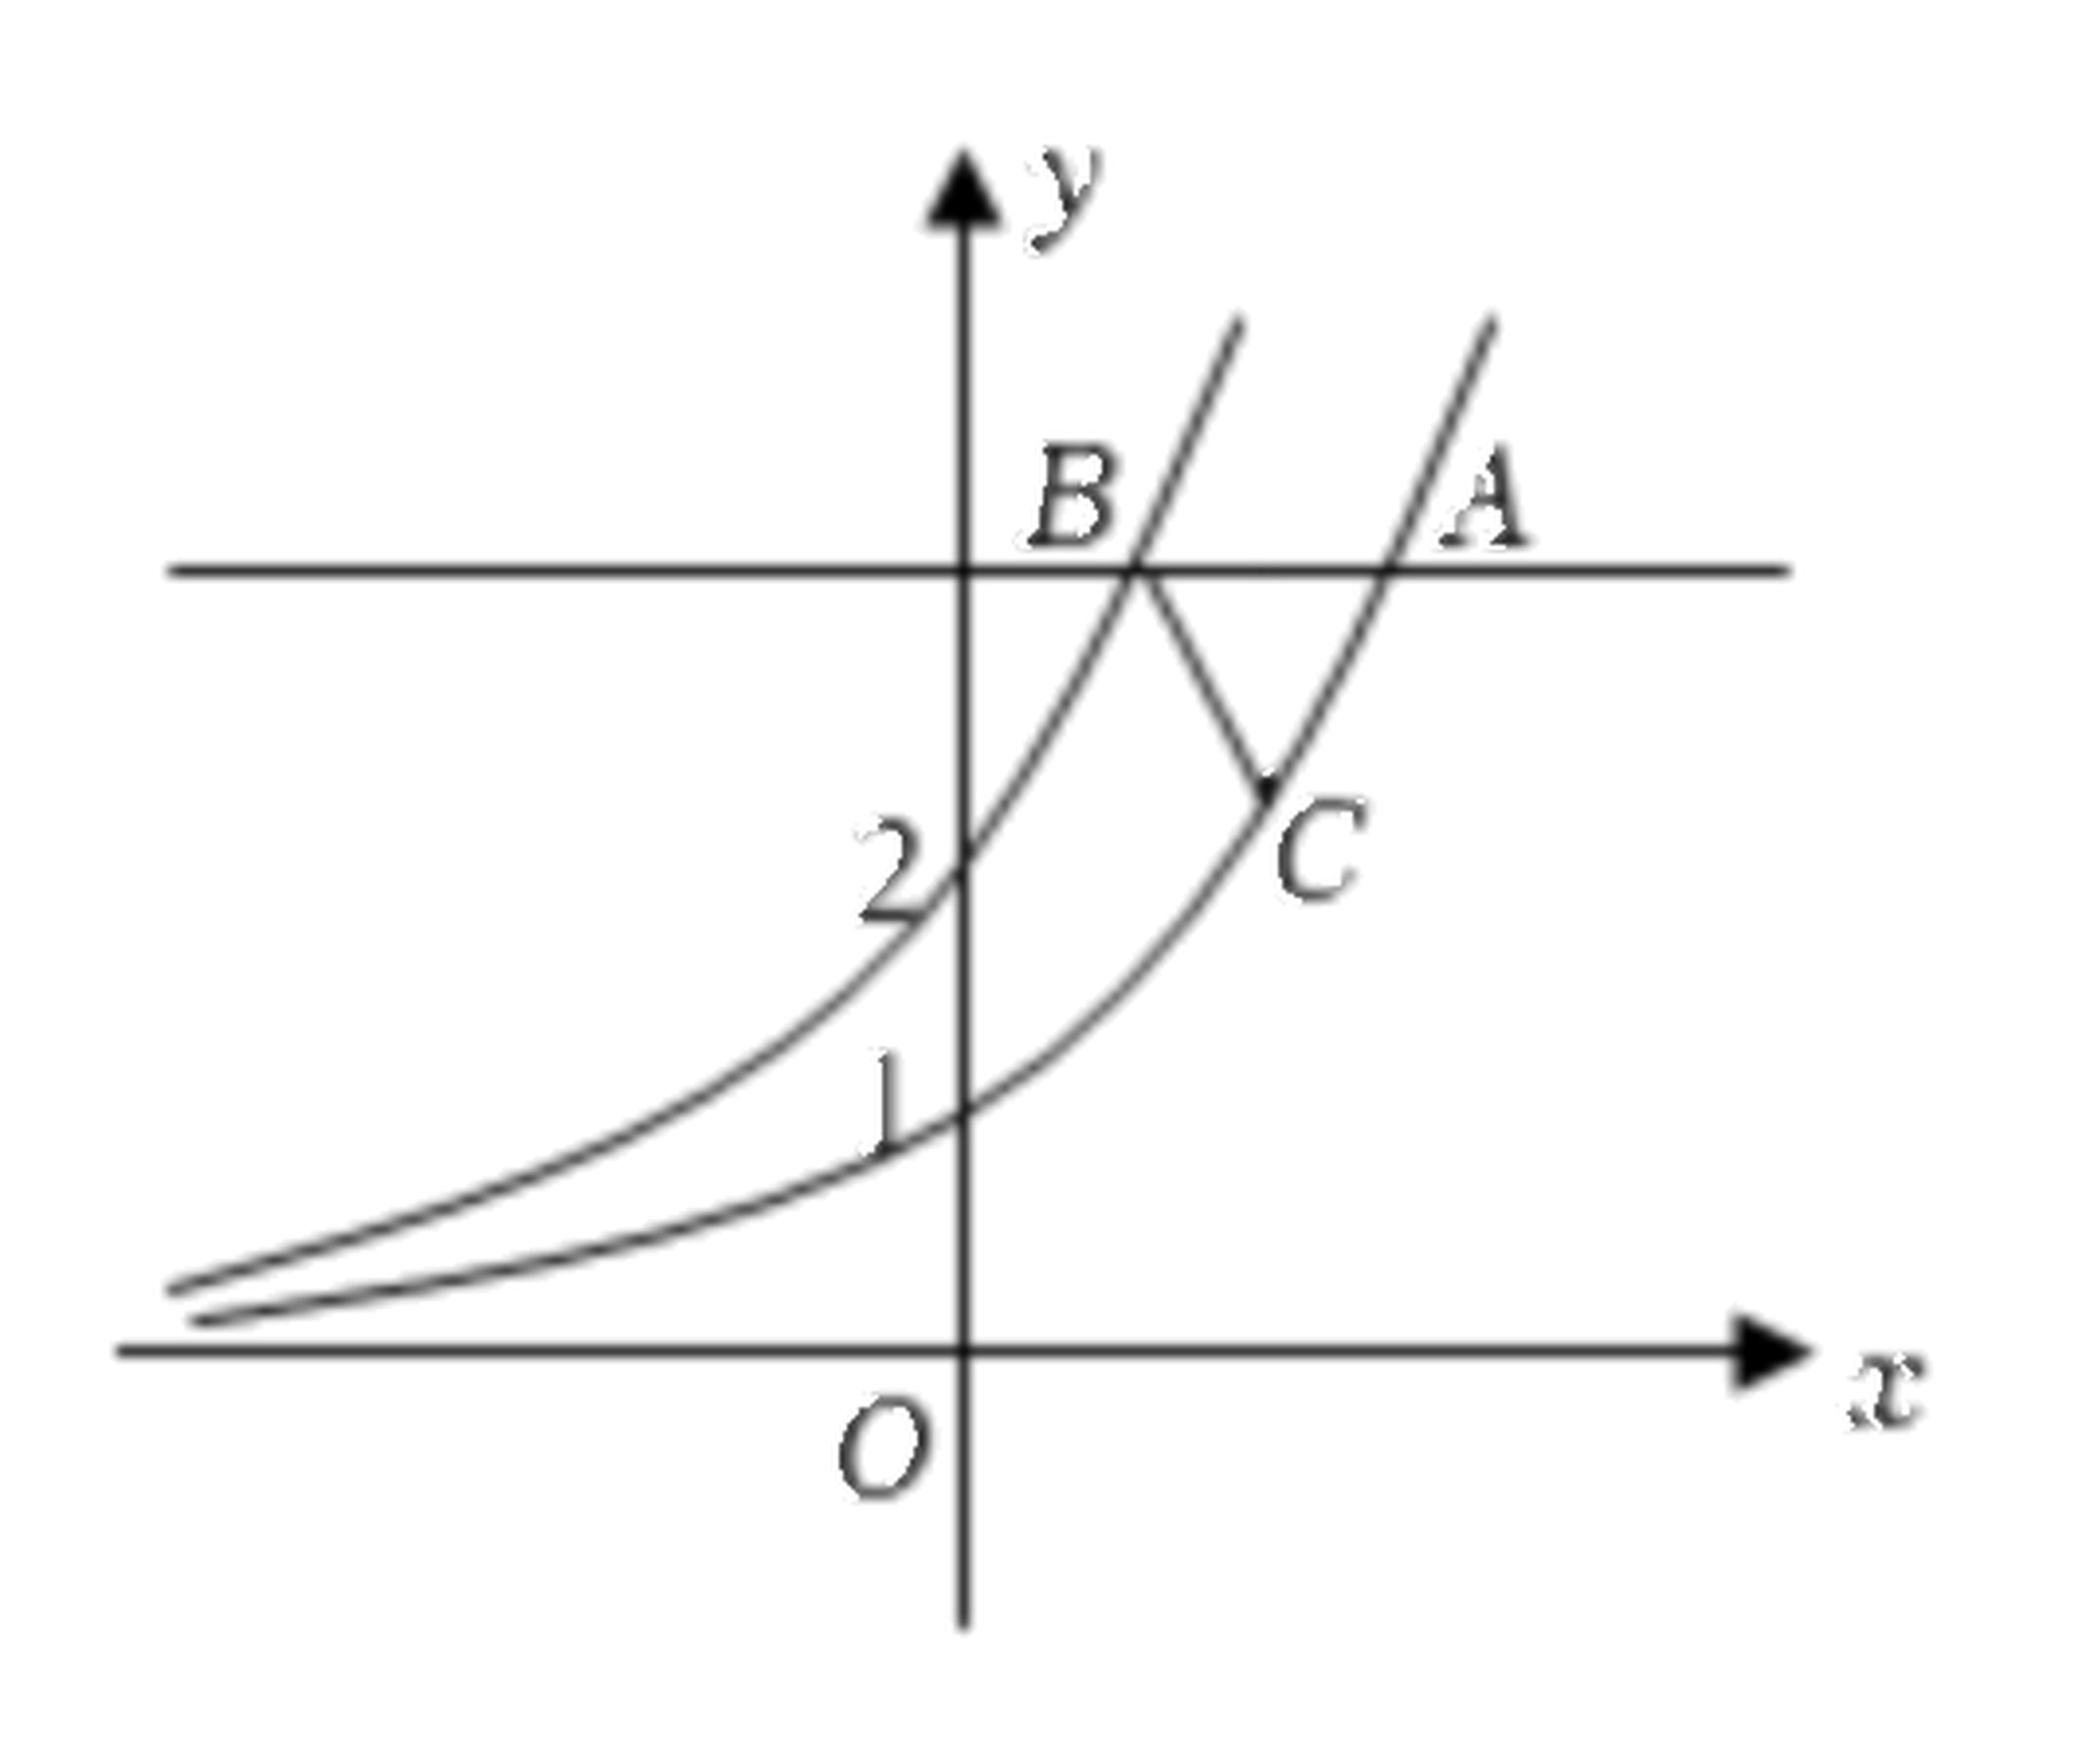
\includegraphics[width=0.40\textwidth]{figures/gao150_q11.png}
\end{center}

\ifanswer
\solbegin
\step{设直线 $l$ 的方程为 $y=a(a>0)$，}
\step{由 $2^x=a$，得 $x=\log_2 a$，所以 $A(\log_2 a,a)$，}
\step{由 $2^{x+1}=a$，得 $x=\log_2 a-1$，所以 $B(\log_2 a-1,a)$，所以 $\lvert AB\rvert=1$，}
\step{取 $AB$ 的中点 $D$，连接 $CD$，如图所示，}
\step{因为 $\triangle ABC$ 为等边三角形，则 $CD\perp AB$，且 $\lvert CD\rvert=\dfrac{\sqrt3}{2}$，}
\step{所以 $C\left(\log_2 a-\dfrac{1}{2},a-\dfrac{\sqrt3}{2}\right)$，}
\step{因为点 $C$ 在函数 $y=2^x$ 的图像上，所以 $a-\dfrac{\sqrt3}{2}=2^{\log_2 a-\frac{1}{2}}=\dfrac{a}{\sqrt2}$，}
\step{解得 $a=\dfrac{\sqrt3}{2-\sqrt2}=\dfrac{\sqrt3(2+\sqrt2)}{4-2}=\sqrt3+\dfrac{\sqrt6}{2}$，}
\step{所以点 $C$ 的纵坐标为 $a-\dfrac{\sqrt3}{2}=\dfrac{\sqrt3+\sqrt6}{2}$.}
\solend
\fi

% === Q12 === 解析配图（高斯函数方格阴影，仅答案版出）；"数学王子"弯引号；cases 块整体算一个印刷行；解析 4 行
\item 小玲在研究数学发展史，特别崇拜近代数学奠基者之一、享有“数学王子”称号的德国数学家高斯. 为了纪念高斯，我们把取整函数 $y=[x]$ 称为高斯函数，其中 $[x]$ 表示不超过 $x$ 的最大整数，如 $[1.1]=1$，$[-1.1]=-2$，则点集 $P=\{(x,y)\mid [x]^2+[y]^2=1\}$ 所表示的平面区域的面积为\blankline[4.4em].

\ifanswer
\solbegin
\step{$[x]^2+[y]^2=1$ 由 $\begin{cases}[x]=0\\ {[y]=-1}\end{cases}$ 或 $\begin{cases}[x]=0\\ {[y]=1}\end{cases}$ 或 $\begin{cases}[x]=-1\\ {[y]=0}\end{cases}$ 或 $\begin{cases}[x]=1\\ {[y]=0}\end{cases}$ 四个平面区域组成，}
\step{即 $\begin{cases}0\leqslant x<1\\ -1\leqslant y<0\end{cases}$ 或 $\begin{cases}0\leqslant x<1\\ 1\leqslant y<2\end{cases}$ 或 $\begin{cases}-1\leqslant x<0\\ 0\leqslant y<1\end{cases}$ 或 $\begin{cases}1\leqslant x<2\\ 0\leqslant y<1\end{cases}$，}
\step{作出平面区域如图所示，平面区域由四个边长为 $1$ 的正方形组成，}
\begin{center}
% 高斯函数 [x]^2+[y]^2=1 方格阴影区域图取 04 页顶部，去粉色水印、去色、4× LANCZOS 放大；仅答案版出
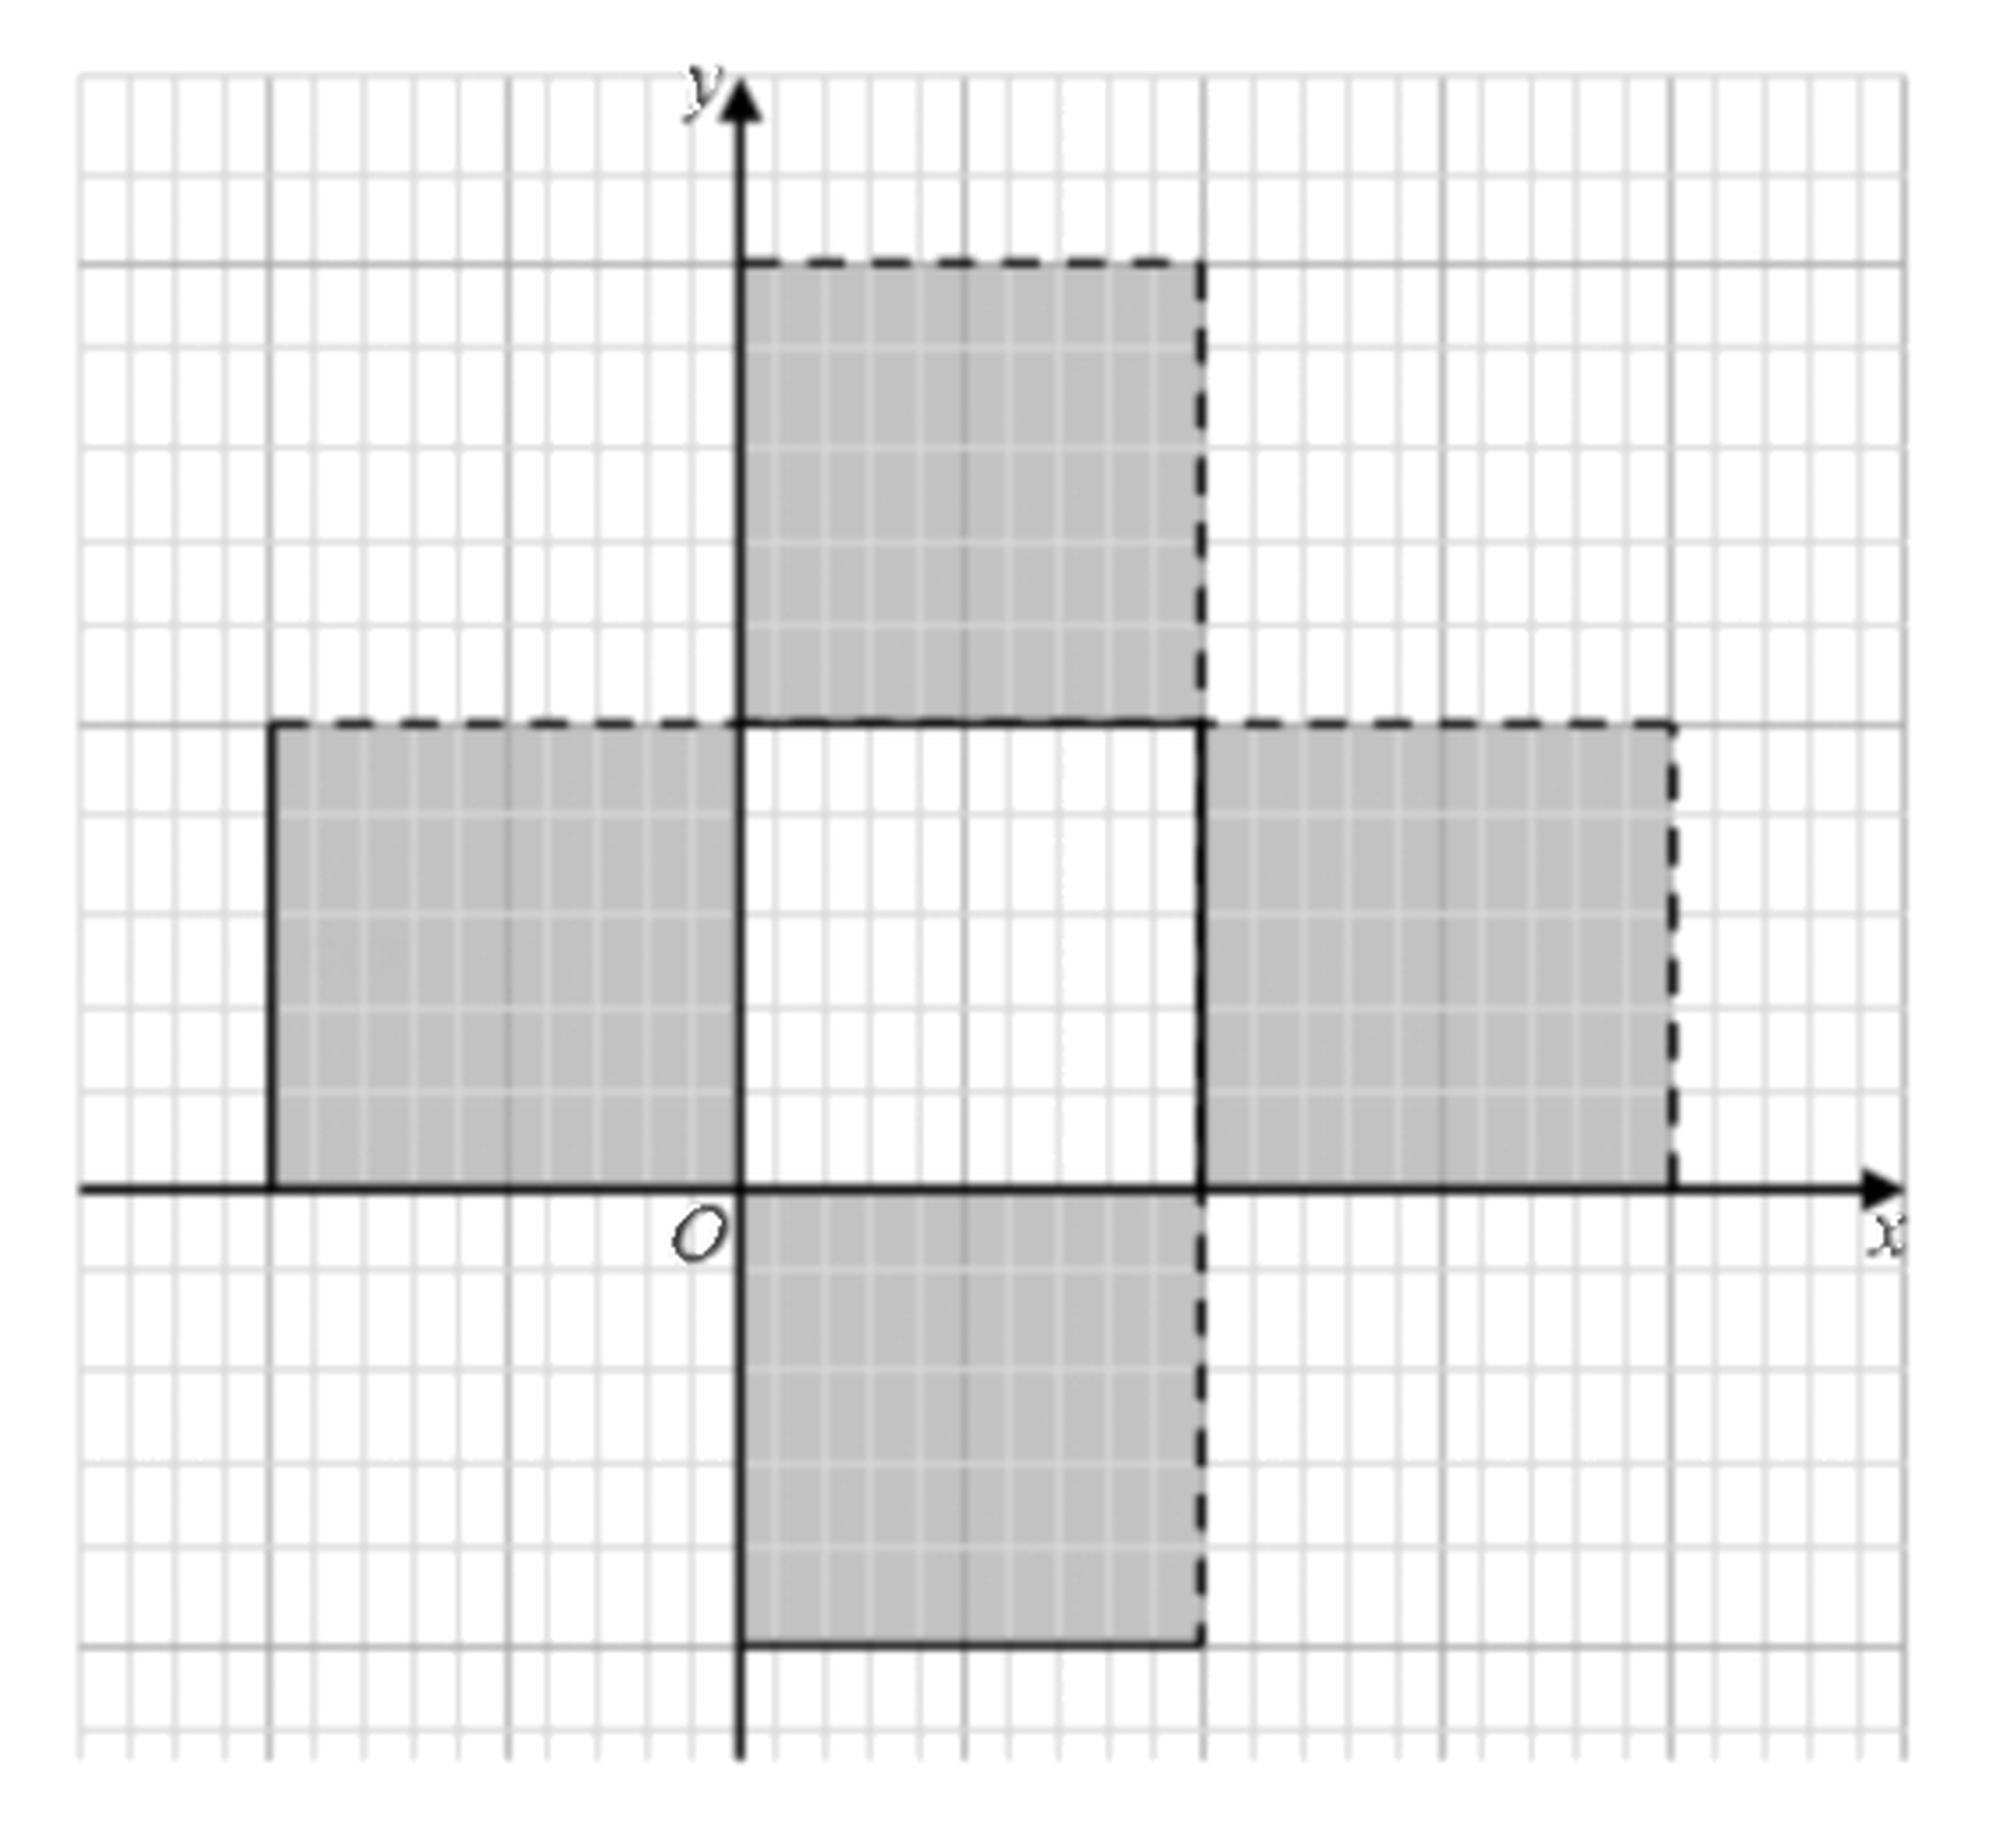
\includegraphics[width=0.34\textwidth]{figures/gao150_q12.png}
\end{center}
\step{总面积为 $1\times4=4$.}
\solend
\fi

\end{enumerate}

\bigsec{二、选择题}

\begin{enumerate}
\setcounter{enumi}{12}

% === Q13 === 答案在解析末句"故选 C"；括号 \mbox{（\quad）} 留空；四选项一行；解析 1 行
\item 设 $x\ne0$，则 $3^{\log_9 x^2}$ 的化简结果是\mbox{（\quad）}

\keepwithprev
A. $x$\qquad B. $\dfrac{1}{x}$\qquad C. $\lvert x\rvert$\qquad D. $\dfrac{1}{\lvert x\rvert}$

\ifanswer
\solbegin
\step{$3^{\log_9 x^2}=3^{\log_3\lvert x\rvert}=\lvert x\rvert$，故选 $C$.}
\solend
\fi

% === Q14 === 题目配图（两函数图像，三版都出）；\needvspace{8cm} 守卫放 \item 之前；"图像"照录；四选项两行两列；解析 2 行，故选 B
\needvspace{8cm}
\item 设 $a>0$ 且 $a\ne1$，$b\in\R$. 若函数 $y=a^{-\lvert x\rvert}$ 与 $y=x^b$ 的大致图像如图所示，则\mbox{（\quad）}

\keepwithprev
A. $0<a<1<b$\qquad\qquad B. $a>1$ 且 $b>1$

C. $0<a<1$ 且 $0<b<1$\qquad\qquad D. $0<b<1<a$

\begin{center}
% 两函数 y=a^{-|x|} 与 y=x^b 大致图像取 04 页右侧，去粉色水印、去色、4× LANCZOS 放大；三版都出
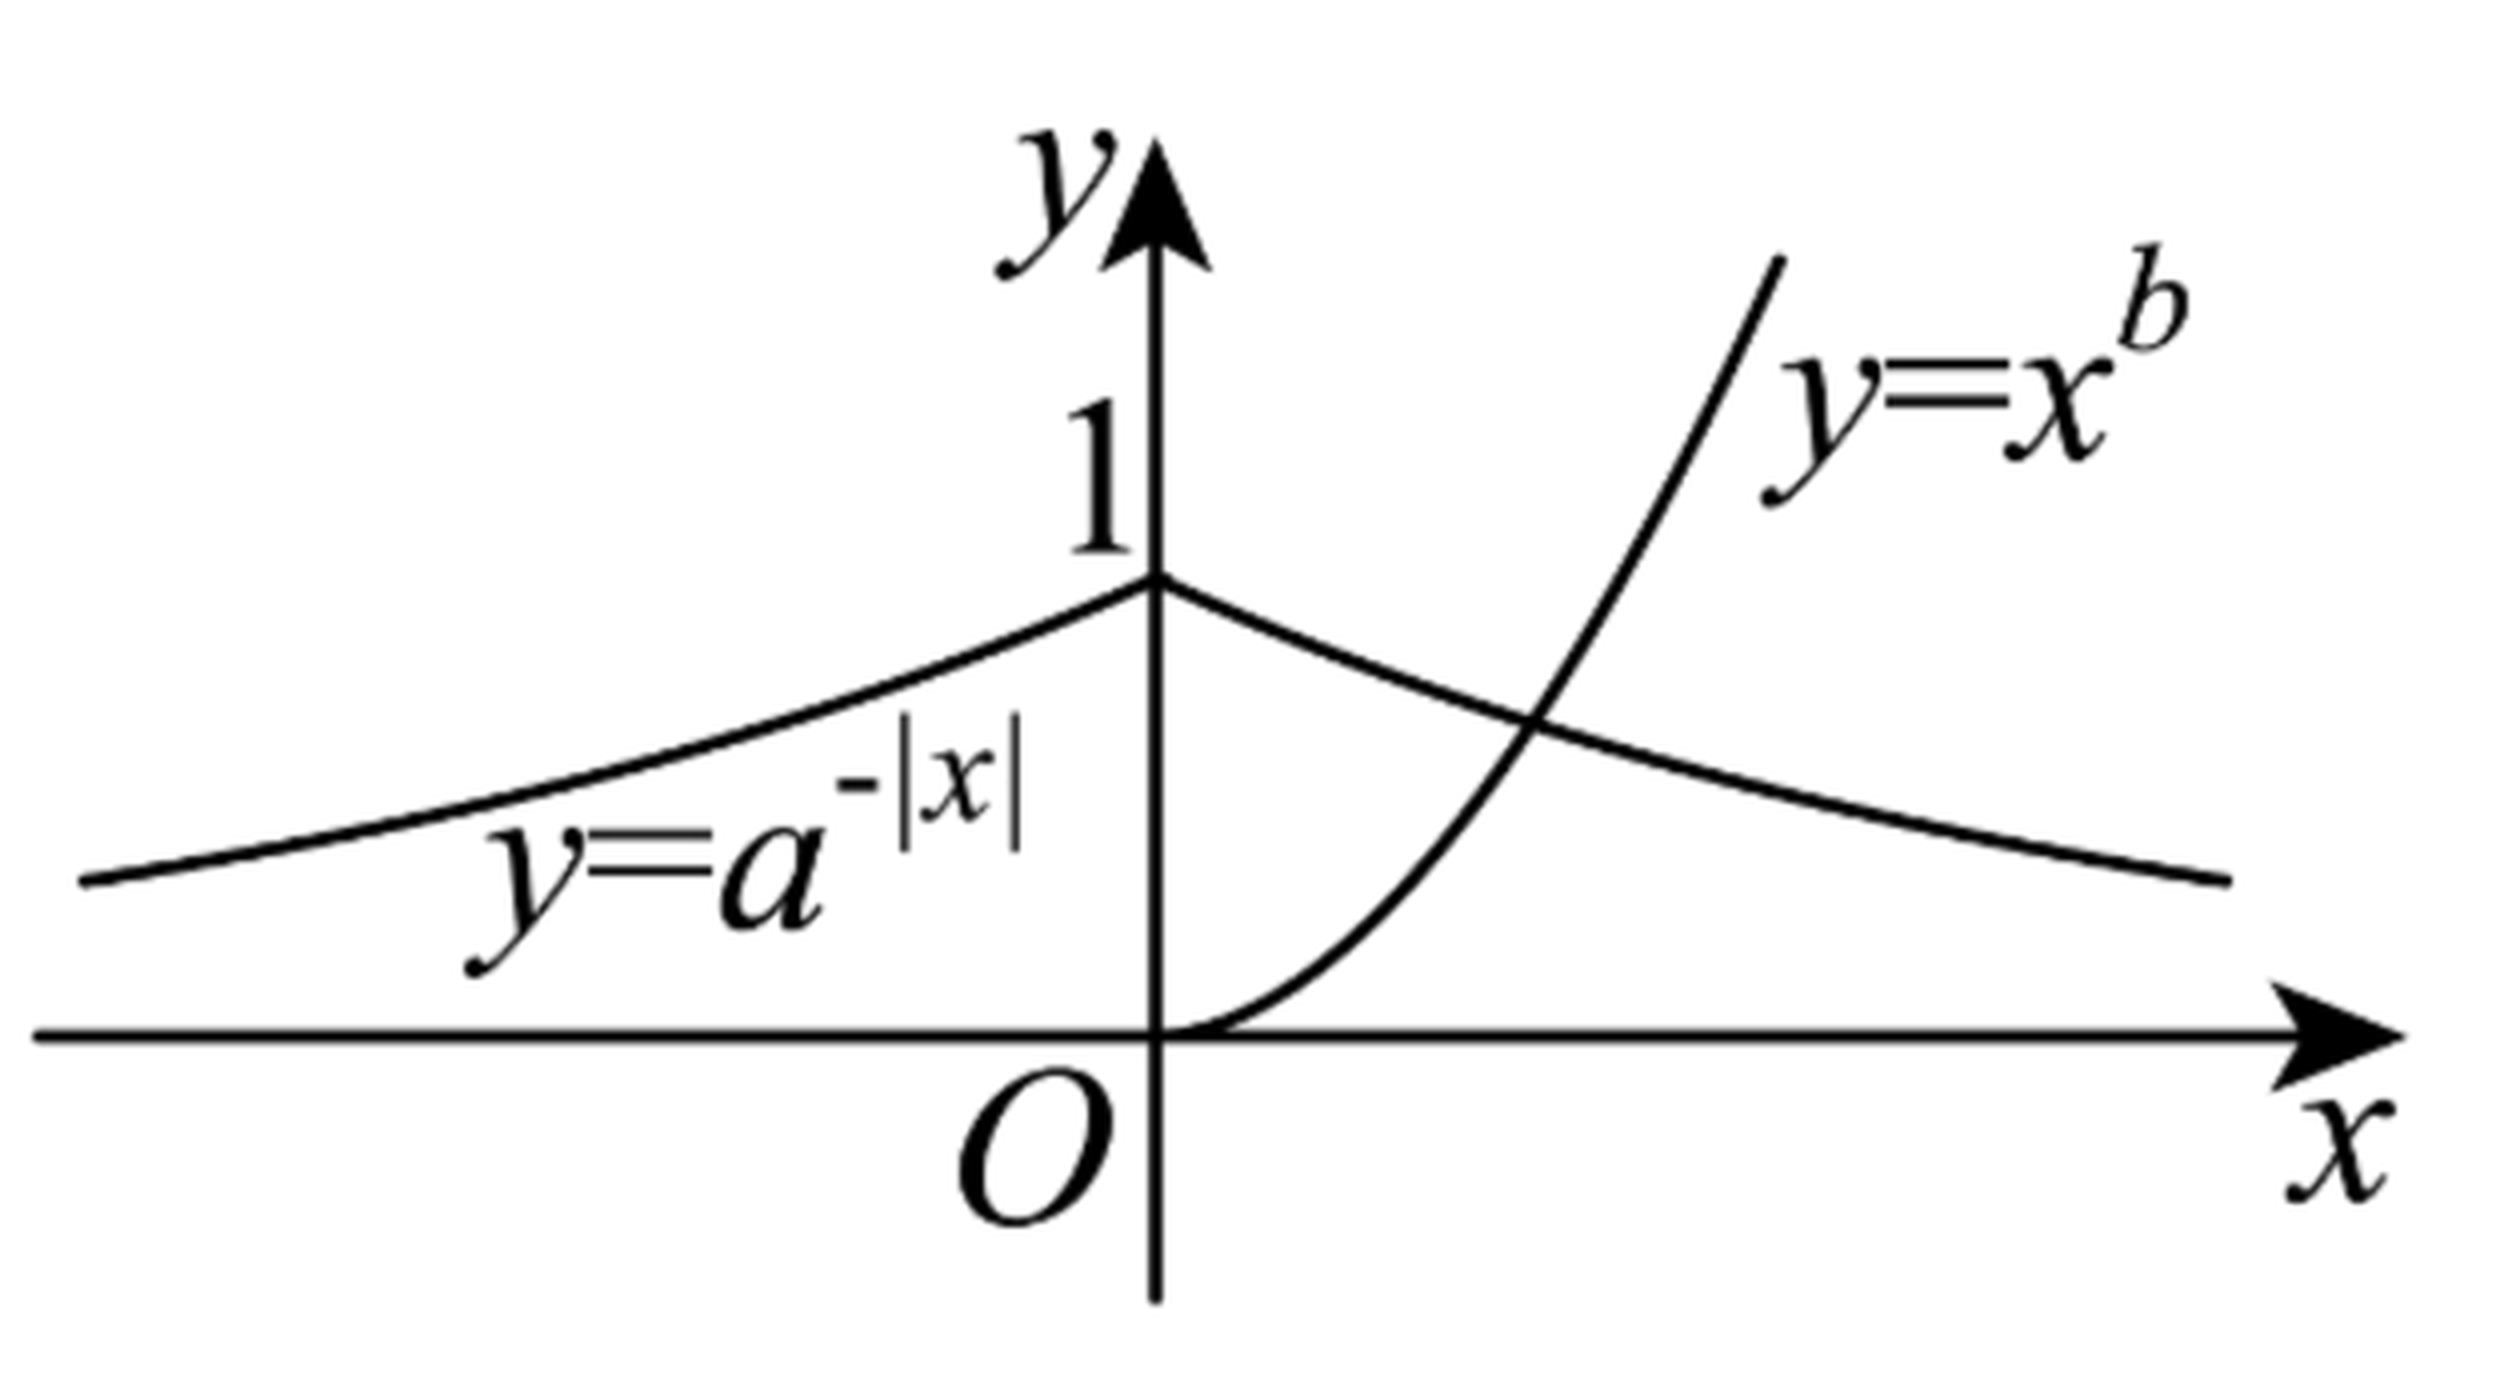
\includegraphics[width=0.40\textwidth]{figures/gao150_q14.png}
\end{center}

\ifanswer
\solbegin
\step{在 $(0,+\infty)$ 上，$y=a^{-x}$ 严格递减，得 $a>1$；}
\step{幂函数 $y=x^b$ 的图像递增且向上弯曲，得 $b>1$；故选 $B$.}
\solend
\fi

% === Q15 === "算术平均值／算术平均数"两处不同照录；四选项两行两列；解析 5 行（续 05 页顶），故选 B
\item 已知两个正数的算术平均值不小于它们的几何平均值，类比有以下结论：三个正数的算术平均数不小于它们的几何平均数，即当 $a,b,c$ 为正实数时，$\dfrac{a+b+c}{3}\geqslant\sqrt[3]{abc}$，当且仅当 $a=b=c$ 时等号成立. 利用上述结论，下列选项中判断正确的是\mbox{（\quad）}

\keepwithprev
A. 若 $x>0$，则 $2x+\dfrac{1}{x^2}\geqslant\dfrac{27}{8}$\qquad\qquad B. 若 $x>0$，则 $x^2+\dfrac{2}{x}\geqslant3$

C. 若 $0<x<1$，则 $x^2(1-x)\geqslant\dfrac{1}{9}$\qquad\qquad D. 若 $0<x<1$，则 $x^2(1-x)\leqslant\dfrac{1}{9}$

\ifanswer
\solbegin
\step{A：取 $x=1$，$2x+\dfrac{1}{x^2}=3<\dfrac{27}{8}$，错误.}
\step{B：$x^2+\dfrac{2}{x}=x^2+\dfrac{1}{x}+\dfrac{1}{x}\geqslant3\sqrt[3]{x^2\cdot\dfrac{1}{x}\cdot\dfrac{1}{x}}=3$，当且仅当 $x=1$ 时取等号，正确.}
\step{C：取 $x=\dfrac{1}{3}$，$x^2(1-x)=\dfrac{2}{27}<\dfrac{1}{9}$，错误.}
\step{D：取 $x=\dfrac{2}{3}$，$x^2(1-x)=\dfrac{4}{27}>\dfrac{1}{9}$，错误.}
\step{故选 $B$.}
\solend
\fi

% === Q16 === "完美集"新定义（弯引号、引号外空格照录）；圈数字①②文本模式；$n\in\N$；四选项两行两列；解析 9 行（6 行 05 页＋3 行 06 页顶），故选 A
\item 已知有限集 $A=\{a_1,a_2,\cdots,a_n\}$（$n\geqslant2$，$n\in\N$）. 若 $A$ 中元素 $a_i$（$i=1,2,\cdots,n$）满足 $a_1+a_2+\cdots+a_n=a_1\cdot a_2\cdots a_n$，就称 $A$ 为 “完美集”. 现有以下两个命题：

①恰有两个元素的 “完美集” 有无穷多个；

②若 $a_i$ 均为正整数，则 “完美集” $A$ 有且只有一个，且 $n=3$.

则\mbox{（\quad）}

\keepwithprev
A. ①和②都是真命题\qquad\qquad B. ①和②都是假命题

C. ①是真命题，②是假命题\qquad\qquad D. ①是假命题，②是真命题

\ifanswer
\solbegin
\step{①由 $a+b=ab\Leftrightarrow(a-1)(b-1)=1$，任取 $a>2$，则 $b=1+\dfrac{1}{a-1}\in(1,2)$，}
\step{得到无穷多个不同的完美集，①真.}
\step{②设 $1\leqslant a_1<a_2<\cdots<a_n$，则 $a_i\geqslant i$.}
\step{若 $n=2$，则 $(a_1-1)(a_2-1)=1$，只能有 $a_1=a_2=2$，与元素互异矛盾.}
\step{若 $n\geqslant4$，则 $a_1a_2\cdots a_n\geqslant a_2a_{n-1}a_n\geqslant2(n-1)a_n>na_n\geqslant a_1+\cdots+a_n$，矛盾.}
\step{当 $n=3$ 时，若 $a_1\geqslant2$，则 $a_1a_2a_3\geqslant6a_3>3a_3\geqslant a_1+a_2+a_3$，矛盾.}
\step{因此 $a_1=1$，$(a_2-1)(a_3-1)=2$，结合 $a_2<a_3$ 得 $a_2=2$，$a_3=3$.}
\step{唯一的完美集为 $\{1,2,3\}$，②真.}
\step{故选 $A$.}
\solend
\fi

\end{enumerate}

\bigsec{三、解答题}

\begin{enumerate}
\setcounter{enumi}{16}

% === Q17 === \varnothing 空集、$B\subseteq A$ 带下划线照录；弯引号内空格照录；解析 7 行
\item 设 $a,b\in\R$. 已知集合 $A=\{x\mid ax^2+3x-a>3\}$，$B=\{x\mid bx=1\}$.

(1) 若 $A=(1,2)$，求 $a$ 的值；

(2) 若 $a=0$，且 “ $x\in A$ ” 是 “ $x\in B$ ” 的必要非充分条件，求 $b$ 的取值范围.

\ifanswer
\solbegin
\step{(1) $A=(1,2)$，则 $a<0$，且 $1,2$ 是方程 $ax^2+3x-a-3=0$ 的两根.}
\step{由 $4a+6-a-3=0$，得 $a=-1$，此时不等式为 $-(x-1)(x-2)>0$，}
\step{解集确为 $(1,2)$.}
\step{(2) $a=0$ 时，$A=(1,+\infty)$，题意等价于 $B\subseteq A$ 且 $B\ne A$.}
\step{当 $b=0$ 时，$B=\varnothing$，符合条件.}
\step{当 $b\ne0$ 时，$B=\left\{\dfrac{1}{b}\right\}$，条件等价于 $\dfrac{1}{b}>1$，解得 $0<b<1$.}
\step{因此 $b$ 的取值范围为 $[0,1)$.}
\solend
\fi

% === Q18 === $p\in\Z$；"图像"（像，有亻）照录；指数 $-2p^2+5p$；解析 8 行（(1) 首行 06 页末＋2 行 07 页顶、(2) 5 行 07 页）
\item 设 $p\in\Z$，已知 $f(x)=x^{-2p^2+5p}$.

(1) 若幂函数 $y=f(x)$ 的图像关于原点成中心对称，且满足 $f(3)<f(4)$，求 $p$ 的值；

(2) 当 $p=-2$ 时，求满足 $f(2x+3)<f(x-4)$ 的 $x$ 的取值范围.

\ifanswer
\solbegin
\step{(1) 图像关于原点成中心对称，得整数 $-2p^2+5p$ 为奇数.}
\step{由 $f(3)<f(4)$，得 $-2p^2+5p>0\Leftrightarrow0<p<\dfrac{5}{2}$，}
\step{结合 $p\in\Z$，得 $p=1$ 或 $p=2$，对应指数分别为 $3$、$2$，所以 $p=1$.}
\step{(2) 当 $p=-2$ 时，$f(x)=\dfrac{1}{x^{18}}$，定义域为 $\{x\in\R\mid x\ne0\}$.}
\step{原不等式要求 $x\ne-\dfrac{3}{2}$ 且 $x\ne4$，}
\step{此时 $\dfrac{1}{(2x+3)^{18}}<\dfrac{1}{(x-4)^{18}}\Leftrightarrow\lvert 2x+3\rvert>\lvert x-4\rvert\Leftrightarrow(2x+3)^2>(x-4)^2$，}
\step{因此 $(x+7)(3x-1)>0\Leftrightarrow x<-7$ 或 $x>\dfrac{1}{3}$，}
\step{排除 $x=4$，得 $x\in(-\infty,-7)\cup\left(\dfrac{1}{3},4\right)\cup(4,+\infty)$.}
\solend
\fi

% === Q19 === $a\in\R$、$g(x)=f(2x+1)+a\cdot f(x)+2$；解析 6 行（(2) 末两行续 08 页顶）
\item 已知 $f(x)=2^x$.

(1) 求方程 $f(2x)-f(x)=6$ 的解；

(2) 设 $a\in\R$，$g(x)=f(2x+1)+a\cdot f(x)+2$，若对于任意 $x\in[-1,1]$，均有 $g(x)\geqslant1$，求 $a$ 的取值范围.

\ifanswer
\solbegin
\step{(1) 令 $t=2^x>0$，则 $t^2-t-6=(t-3)(t+2)=0$，}
\step{由 $t>0$ 得 $t=3$，所以 $x=\log_2 3$.}
\step{(2) 令 $t=2^x$，则 $t\in\left[\dfrac{1}{2},2\right]$，且 $g(x)\geqslant1\Leftrightarrow2t^2+at+1\geqslant0\Leftrightarrow a\geqslant-\left(2t+\dfrac{1}{t}\right)$，}
\step{由基本不等式得 $2t+\dfrac{1}{t}\geqslant2\sqrt{2t\cdot\dfrac{1}{t}}=2\sqrt2$，}
\step{当且仅当 $t=\dfrac{1}{\sqrt2}\in\left[\dfrac{1}{2},2\right]$ 时等号成立，}
\step{因此 $-\left(2t+\dfrac{1}{t}\right)$ 的最大值为 $-2\sqrt2$，所求范围为 $a\in[-2\sqrt2,+\infty)$.}
\solend
\fi

% === Q20 === "极闭集"新定义、3 问，全卷末题；$M\subseteq(0,+\infty)$ 带下划线照录；自定义运算 $x*y$ 星号照录；解析 13 行（9 行 08 页＋4 行 09 页上半）
\item 对于非空实数集 $M\subseteq(0,+\infty)$，若满足以下两个条件：

① $M$ 中至少含有 $2$ 个元素，且 $1\notin M$；

②对于 $M$ 中任意两个不相等的元素 $x$、$y$，定义 $x*y=\dfrac{xy+1}{x+y}$，且 $x*y\in M$.

则称 $M$ 为 “极闭集”.

(1) 分别判断集合 $A=\left\{\dfrac{1}{2},3\right\}$ 与集合 $B=(1,+\infty)$ 是否为 “极闭集” （无需理由）；

(2) 若 $M$ 是 “极闭集”，证明：$M$ 中不可能所有元素都小于 $1$；

(3) 证明：不存在任何有限集是 “极闭集”.

\ifanswer
\solbegin
\step{(1) $A$ 不是 “极闭集”，$B$ 是 “极闭集”.}
\step{(2) 假设 $M$ 中所有元素都小于 $1$，取其中两个不相等的元素 $x$、$y$，}
\step{则 $x*y-1=\dfrac{(1-x)(1-y)}{x+y}>0$，}
\step{这与 $x*y\in M$ 且 $M$ 中所有元素都小于 $1$ 矛盾.}
\step{(3) 假设有限集 $M$ 是 “极闭集”，}
\step{由 (2) 及 $1\notin M$，得 $M$ 中存在大于 $1$ 的元素.}
\step{若 $M$ 中有小于 $1$ 的元素，取其中最大的一个为 $a$，另取 $b\in M$ 且 $b>1$，}
\step{则 $a*b-a=\dfrac{1-a^2}{a+b}>0, a*b-1=\dfrac{(a-1)(b-1)}{a+b}<0$，}% 半角逗号在两个数学式组之间，全稿惯例、非笔误，照录
\step{于是 $a<a*b<1$ 且 $a*b\in M$，与 $a$ 的最大性矛盾.}
\step{若 $M$ 中没有小于 $1$ 的元素，则 $M\subseteq(1,+\infty)$.}
\step{取 $a=\min M$，另取 $b\in M$ 且 $b\ne a$，则 $a*b-a=\dfrac{1-a^2}{a+b}<0$，}
\step{于是 $a*b<a$ 且 $a*b\in M$，与 $a$ 的最小性矛盾.}
\step{因此不存在任何有限集是 “极闭集”.}
\solend
\fi

\end{enumerate}

\end{document}
"
% 紧凑版：xelatex "\def\iscompact{1}% 高一150_曹杨二中_期中.tex
%   —— 高一上数学"2026-2027 年曹杨二中高一上期中"（试卷版/答案版/紧凑版）
% 试卷版：xelatex 高一150_曹杨二中_期中.tex
% 答案版：xelatex "\def\isanswer{1}\input{高一150_曹杨二中_期中.tex}"
% 紧凑版：xelatex "\def\iscompact{1}\input{高一150_曹杨二中_期中.tex}"
%
% ① 原始材料：微信公众号"魔都数学加油站"文章，连载"27学年高一150"，原文标题
% "27学年高一150——2026-2027年上海市曹杨二中高一上期中"；
% 原文链接：https://mp.weixin.qq.com/s/xlQxmik8TZXR87RC6MnCrw 。
% 正文为 9 张 PNG 页（01/02/04/06/07/09 为 2560×3620，03/05/08 为 4762×6735，
% 同一篇各页分辨率混排，逐页按各自分辨率裁图核对，别按预览比例换算裁框）。
% 体例：讲评版——全 18 题均印【解析】（逐题核实，见 ② ②）。
% 题目、答案、解析均据原图转录；卷面粉红色/红色水印"魔都数学加油站"及公众号页脚未录入。
% 全卷插图清单（逐页通读 9 页确认）：3 幅——
%   · Q11 题目配图（指数函数曲线图，02 页右侧：x/y 轴、O、y=2^x 与 y=2^{x+1}
%     两曲线、A/B/C 三点、刻度 1/2、等边三角形 ABC），三版都出，裁 figures/gao150_q11.png；
%   · Q12 解析配图（高斯函数取整 [x]^2+[y]^2=1 方格阴影区域图，04 页顶部：4 个边长 1
%     的正方形组成的十字形阴影），解析"作出平面区域如图所示"处，仅答案版出，
%     放 \ifanswer 内 \step 之间，裁 figures/gao150_q12.png；
%   · Q14 题目配图（两函数 y=a^{-|x|} 与 y=x^b 大致图像，04 页右侧：x/y 轴、O、
%     y 轴刻度 1、一递减曲线一递增上翘曲线），三版都出，裁 figures/gao150_q14.png；
%   其余各页逐页确认无其它题目配图、无表格；Q11/Q12 解析"如图所示"对应的就是上列
%   已裁的图，不重复裁；09 页上半为 Q20(3) 解析续尾、下半仅水印、无正文。
%   3 图均取自原卷截图，去粉色水印、去色、4× LANCZOS 放大。
%
% 卷首标题：原卷印作"2026-2027 年曹杨二中高一上期中"，年份区间按全稿惯例排 en dash；
% 原卷卷面未印副标题，本稿按同期中卷知识模块口径补出"集合与常用逻辑用语、不等式、函数"。
%
% 题号体例（逐页核实定稿）：本卷共 18 题——一、填空题 3—12（10 题）、
% 二、选择题 13—16（4 题）、三、解答题 17—20（4 题）。
% 三节分别 \setcounter{enumi}{2}／{12}／{16}。原卷从第 3 题起、无第 1、2 题，
% 本稿保留原题号；全卷末题为第 20 题（"极闭集"新定义、3 问），无 Q21、无附加题节。
%
% ② 与原卷的排版差异：
%   ① 原文从第 3 题起，本稿保留原题号；共 18 题三节，解答题只有 4 题到 20；
%   ② 全 18 题均印【解析】，用 \solbegin…\solend；逐题核实无只印【答案】或
%      答案印题干括号内的题；四道选择题答案在解析末句"故选 X"（Q13 选 C、
%      Q14 选 B、Q15 选 B、Q16 选 A，逐个放大复核）、括号 \mbox{（\quad）} 留空、
%      不另提 \ans{}；答案版【答案】/【解析】标记数 = 18 = 全卷题数；
%   ③ 原卷卷面未印副标题，本稿按知识模块口径补出；
%   ④ 原卷填空横线按全稿惯例排 \blankline[4.4em]；选择题括号排 \mbox{（\quad）}、
%      选项段前按惯例加 \keepwithprev；解答题不留作答区、不加 \anspace（原卷为讲评版）；
%   ⑤ 数集黑板粗体：Q4"m\in R"、Q5"a,b\in R"、Q6"a,b,c\in R"、Q7"a\in R"、
%      Q10"a\in R"、Q14"b\in R"、Q17"a,b\in R"、Q18"p\in Z"／定义域"x\in R"、
%      Q19"a\in R"、Q16"n\in N" 原卷印斜体 R/Z/N，按全稿惯例归一 \R／\Z／\N；
%      绝对值排 \lvert…\rvert（Q7 |x+4|+|x-3|、Q11 |AB|／|CD|、Q13 |x|、
%      Q18 |2x+3|／|x-4|），集合描述竖线排 \mid（Q3、Q12、Q17、Q18、Q20），
%      不等号按全稿惯例排 \leqslant／\geqslant；补集照原卷上划线排 \overline{A}
%      （Q3 题干＋解析共 2 处）；空集符号 \varnothing（Q17 解析(2)）；
%      子集 \subset（单线⊂）／\subseteq（带下划线⊆）逐处照录，本卷 3 处子集
%      符号均印带下划线 ⊆、照录 \subseteq（Q20 题干、Q20 解析(3)、Q17 解析(2)，
%      见 ④），无 \subset 用例；
%   ⑥ 判别式 Δ/△：逐页通读 9 页，本卷无一元二次判别式算式，故无 Δ/△ 混用可照录
%      （"高 \Delta／扁 \triangle"口径备查，参照 高一142／144／145／146／148／149
%      头注④）；本卷仅 Q11 题干与解析共 2 处几何三角形符号 △ABC，逐处放大并排
%      确认两处同形、印近等边粗线三角（非判别式），照录 \triangle（见 ④）；
%   ⑦ 中文弯引号照录：Q12"数学王子"、Q16"完美集"（题干＋①②两命题，引号外
%      留空格）、Q17" x∈A "" x∈B "（引号内空格）、Q20"极闭集"（题干条件、
%      三问与解析，引号外留空格）；注释里一律 ASCII 引号；数学式内 CJK 用 \text{}
%      （Q3 集合描述"且"用 \text{ 且 }）；
%   ⑧ 半角逗号在数学组之间是全稿惯例、非笔误，逐处照录（Q17 解析"1,2 是方程…
%      两根"、Q20 解析(3)">0, a*b-1=…<0" 两式之间等）；行末西文句点 ASCII `.`；
%      行中全角逗号／顿号照录（Q12"之一、享有"、Q18 解析"3、2"、Q20"x、y"）；
%   ⑨ "图像／图象"逐处放大核：全卷 9 处均印"图像"（像，有亻）、未见"图象"——
%      Q4 题干 1、Q11 题干 2＋解析 1、Q14 题干 1＋解析 1、Q18 题干 1＋解析 1；
%      同卷"第二象限""象限"用"象"（无亻）。逐处照录未统一改动（放大 01/02/04/06
%      页 /tmp/gao150/z/p01_q4_tuxiang2.png、p04_q14_tuxiang2.png、
%      p02_q11_lines.png 确认）；子题标号 (1)(2)(3) 半角括号照录；圈数字①②
%      在文本模式（Q16 两命题与解析、Q20 两条件与三问及解析）按 common.sty
%      划入 CJK 字符类渲染，进数学式用 \text{①}；
%   ⑩ Q20 新定义 x*y=\dfrac{xy+1}{x+y} 的 * 是自定义运算（星号），照录；
%      \left…\right 不得拆到不同 $…$ 组（Q19"\left(2t+\frac1t\right)"、
%      Q20 题干"A=\left\{\frac12,3\right\}"等）；Q8 嵌套根号
%      \sqrt{\frac2x+\frac{16}{1-2x}}、Q9 对数连加 \log_2 A 等复杂式照录别简化；
%   ⑪ 一条 \step = 原卷解析的一个印刷行，cases 块整体算一个印刷行；别并折行、
%      别拆行。Q4 三行、Q8 五行、Q11 九行、Q12 四行（两行各含四个 cases 块）、
%      Q15 五行、Q16 九行、Q18 八行、Q20 十三行均按印刷行逐条断，不丢行；
%   ⑫ 配图：Q11／Q14 题目配图（三版都出）放 \item 内题干之后 \begin{center}，
%      大图块加 \needvspace{8cm} 守卫把整块推走（守卫放 \item 之前，见
%      高一145 Q14/Q20 成例与切页审计 B 类坑）；Q12 解析配图（仅答案版出）
%      放 \ifanswer 内 \solbegin…\solend 的 \step 之间（高一73 第16题成例）；
%   ⑬ 跨页续印按题合并：见 ⑥；
%   ⑭ 原卷解析内无红色"法一／法二"之类小标题，故本卷无 \stepm；红色水印
%      "魔都数学加油站"不录入；Q12 解析"作出平面区域如图所示"对应的图即
%      ① 所列 gao150_q12.png（04 页顶部），不重复裁；Q11 解析"如图所示"对应
%      题目配图 gao150_q11.png，不另裁。
%
% ③ 行数复核：一条 \step／\stepm = 原卷解析的一个印刷行，cases 块作一个印刷行计。
%   逐题数（主会话逐页核对定稿）：Q3：1；Q4：3；Q5：2；Q6：1；Q7：2；Q8：5；
%   Q9：1；Q10：3；Q11：9；Q12：4；Q13：1；Q14：2；Q15：5；Q16：9；
%   Q17：7；Q18：8；Q19：6；Q20：13。
%   合计 82 条 \step（本卷无 \stepm：解析内无红色"法一／法二"类小标题），
%   与原卷逐题印刷行相等。全卷 18 题均设 \solbegin…\solend，答案版
%   【答案】/【解析】标记数 = 18 = 全卷题数。
%
% ④ 判别式／三角形／子集符号结论（逐处放大原图照录、不得统一，主会话像素级复核）：
%   判别式：逐页通读 9 页，本卷无一元二次判别式 Δ/△ 算式（Q18 讨论幂函数指数
%     奇偶、不用判别式；Q9／Q19／Q20 亦无），头注 ② ⑥ 的"高 \Delta／扁 \triangle"
%     口径在本卷无对应处（参照 高一142／144／145／146／148／149 头注④，仅备查）。
%   几何三角形符号：Q11 题干"使得 △ABC 为等边三角形"（02 页末）与解析
%     "因为 △ABC 为等边三角形，则 CD⊥AB"（03 页）共 2 处，放大 02/03 页
%     /tmp/gao150/z/q11_tri_montage2.png 并排确认两处同形、印近等边粗线三角
%     （h/w≈0.98、非"高>宽"的判别式 \Delta），照录 \triangle（与 高一105
%     "使得 \triangle ABC 为等边三角形" 同短语成例、高一149 几何三角形照录
%     \triangle 口径一致），不引入 \Delta。
%   子集／补集：Q20 题干"$M\subseteq(0,+\infty)$"（08 页）、Q20 解析(3)
%     "则 $M\subseteq(1,+\infty)$"（09 页）、Q17 解析(2)"题意等价于 $B\subseteq A$
%     且 $B\ne A$"（06 页）共 3 处子集符号，逐处放大（/tmp/gao150/z/p08_q20_stem.png、
%     p09_q20_sub.png、p06_q17_sub.png）确认均印带下划线 ⊆，照录 \subseteq；
%     本卷未见单线 ⊂（\subset）之对应处。Q3 题干与解析共 2 处补集照原卷上划线
%     排 \overline{A}；Q17 解析(2) 空集印 ∅、照录 \varnothing（Q7"解集为空集"
%     为中文词、非符号，照录文字）；集合描述竖线 \mid；数集 \R／\Z／\N 归一见 ② ⑤。
%
% ⑤ 存疑照录（放大原图确认，照录未改、正文对应处另有 % 注）：
%   1. Q8 解析第 4 行"所以 $y=\frac1x+\frac{8}{1-2x}$ 的最小值为 18" —— 上文
%      并未定义 $y$，且题面求的是 $\sqrt{\frac2x+\frac{16}{1-2x}}$ 的最小值；
%      按上下文该行应为 $\frac1x+\frac{8}{1-2x}$ 的最小值为 18（$y$ 疑为原卷
%      衍字／笔误），放大 02 页 /tmp/gao150/z/p02_q8_y.png 确认，照录未改。
%   2. Q20 解析(3)"$a*b-a=\frac{1-a^2}{a+b}>0, a*b-1=\frac{(a-1)(b-1)}{a+b}<0$"
%      两式之间的逗号原卷印半角 ,（非全角），按全稿惯例"半角逗号在数学组之间"
%      照录未改（放大 08 页 /tmp/gao150/z/p08_q20_sol8.png 确认）。
%   3. Q15 题干"两个正数的算术平均值…几何平均值"与"三个正数的算术平均数…
%      几何平均数"两处"值／数"用字不同，逐处照录未统一（放大 04 页确认）。
%   4. "图像／图象"全卷 9 处均印"图像"（像，有亻）、未见"图象"，逐处放大核实
%      照录、未统一改动（见 ② ⑨）；本卷判别式 Δ/△ 无用例、几何三角形 2 处
%      照录 \triangle（见 ④）。
%   全卷除此 4 类外未发现其它笔误／自相矛盾处；18 题均印【解析】、无只印【答案】
%   或答案印题干括号内的题（见 ② ②）。
%
% ⑥ 跨页续印按题合并说明（逐页核实定稿）：Q3/4/5/6/7 题干＋解析在 01 页；
%   Q8 题干＋解析 5 行、Q9 题干＋解析 1 行在 02 页上半；Q10 题干＋解析 3 行
%   在 02 页下半；Q11 题干（前两行）＋配图在 02 页下半、题干续"三角形，则点 C
%   的纵坐标为___"与解析 9 行全在 03 页上半（解析"如图所示"对应题目配图）；
%   Q12 题干＋解析 4 行在 03 页下半，解析配图（方格阴影）续印在 04 页顶部；
%   "二、选择题"标题在 04 页中部；Q13 题干＋选项＋解析、Q14 题干＋选项＋
%   配图＋解析在 04 页；Q15 题干＋四选项在 04 页末、解析 5 行续 05 页上半；
%   Q16 题干＋①②两命题＋"则(  )"＋四选项＋解析前 6 行在 05 页、解析末 3 行
%   （"因此 a_1=1…②真""故选 A"）续 06 页顶部；"三、解答题"标题在 06 页；
%   Q17 题干(1)(2)＋解析(1) 3 行＋解析(2) 首行在 06 页、解析(2) 续 3 行
%   在 06 页下半；Q18 题干(1)(2)＋解析(1) 首行在 06 页末、解析(1) 续 2 行＋
%   解析(2) 5 行在 07 页上半；Q19 题干(1)(2)＋解析(1) 2 行＋解析(2) 前 2 行
%   在 07 页下半、解析(2) 末 2 行续 08 页顶部；Q20 题干（新定义＋①②两条件）
%   ＋三问＋解析(1)(2)(3) 前 9 行在 08 页、解析(3) 末 4 行续 09 页上半，
%   末行"因此不存在任何有限集是极闭集"为全卷收尾（09 页下半仅水印、无正文）。
%   本稿按题连排，不丢行、不并折行；全卷末题为第 20 题，无 Q21、无附加题节。
%
\documentclass[a4paper,11pt]{article}
\usepackage{common}

\begin{document}

\examtitlest[3]{2026--2027 年曹杨二中高一上期中}{集合与常用逻辑用语、不等式、函数}

\bigsec{一、填空题}

\begin{enumerate}
\setcounter{enumi}{2}

% === Q3 === 补集上划线 \overline{A}（题干＋解析各 1 处）；集合描述竖线 \mid、数学式内"且"用 \text{}；解析 1 行
\item 设全集 $U=\{1,2,3,4,5\}$，集合 $A=\{x\mid x^2-3x\leqslant0\text{ 且 }x\in U\}$，则 $\overline{A}=$\blankline[4.4em].

\ifanswer
\solbegin
\step{$x^2-3x\leqslant0\Leftrightarrow0\leqslant x\leqslant3$，所以 $A=\{1,2,3\}$，$\overline{A}=\{4,5\}$.}
\solend
\fi

% === Q4 === "图像"（像，有亻）逐处照录、同句"第二象限"用"象"（无亻）；解析 3 行
\item 设 $m\in\R$. 若幂函数 $y=(m^2-5m+1)x^{m+1}$ 的图像经过第二象限，则 $m=$\blankline[4.4em].

\ifanswer
\solbegin
\step{幂函数的系数为 1，故 $m^2-5m+1=1\Rightarrow m=0$ 或 $m=5$.}
\step{$m=0$ 时，$y=x$ 不经过第二象限；}
\step{$m=5$ 时，$y=x^6$ 经过第二象限，因此 $m=5$.}
\solend
\fi

% === Q5 === 解析 2 行
\item 设 $a,b\in\R$. 若 $a^2+\dfrac{b^2}{4}=1$，则 $ab$ 的最大值为\blankline[4.4em].

\ifanswer
\solbegin
\step{$1-ab=\left(a-\dfrac{b}{2}\right)^2\geqslant0$，即 $ab\leqslant1$；}
\step{当 $a=\dfrac{\sqrt2}{2}$，$b=\sqrt2$ 时取等号，最大值为 1.}
\solend
\fi

% === Q6 === 解析 1 行
\item 设 $a,b,c\in\R$. 若等式 $2x^2-3x-2=a(x-1)^2+b(x-1)+c$ 恒成立，则 $a-b+c=$\blankline[4.4em].

\ifanswer
\solbegin
\step{令 $x=0$，得 $a-b+c=-2$.}
\solend
\fi

% === Q7 === 绝对值 \lvert…\rvert；解析 2 行
\item 设 $a\in\R$. 若关于 $x$ 的不等式 $\lvert x+4\rvert+\lvert x-3\rvert<a$ 的解集为空集，则 $a$ 的取值范围是\blankline[4.4em].

\ifanswer
\solbegin
\step{$\lvert x+4\rvert+\lvert x-3\rvert\geqslant\lvert(x+4)-(x-3)\rvert=7$，当 $-4\leqslant x\leqslant3$ 时取等号.}
\step{原不等式的解集为空集当且仅当 $a\leqslant7$，即 $a\in(-\infty,7]$.}
\solend
\fi

% === Q8 === 嵌套根号 \sqrt{\frac{2}{x}+\frac{16}{1-2x}} 照录别简化；解析 5 行
\item 设 $x\in\left(0,\dfrac{1}{2}\right)$，则 $\sqrt{\dfrac{2}{x}+\dfrac{16}{1-2x}}$ 的最小值为\blankline[4.4em].

\ifanswer
\solbegin
\step{因为 $x\in\left(0,\dfrac{1}{2}\right)$，所以 $1-2x>0$，又 $2x+1-2x=1$，}
\step{所以 $\left(\dfrac{1}{x}+\dfrac{8}{1-2x}\right)(2x+1-2x)=10+\dfrac{1-2x}{x}+\dfrac{16x}{1-2x}$}
\step{$\geqslant10+2\sqrt{\dfrac{1-2x}{x}\cdot\dfrac{16x}{1-2x}}=18$，}
\step{当且仅当 $\dfrac{1-2x}{x}=\dfrac{16x}{1-2x}$ 即 $x=\dfrac{1}{6}$ 时取等号，所以 $y=\dfrac{1}{x}+\dfrac{8}{1-2x}$ 的最小值为 18，}% 原卷此处径写 $y=\frac1x+\frac{8}{1-2x}$（上文未定义 $y$、且与题面根式不符），疑笔误，放大 02 页确认，照录未改（见 ⑤）
\step{所以 $\sqrt{\dfrac{2}{x}+\dfrac{16}{1-2x}}$ 的最小值为 6.}
\solend
\fi

% === Q9 === 对数连加 \log_2 A 等复杂式照录别简化；解析 1 行
\item 记 $A=1\times2\times3\times\cdots\times2026$，则 $\dfrac{1}{\log_2 A}+\dfrac{1}{\log_3 A}+\dfrac{1}{\log_4 A}+\cdots+\dfrac{1}{\log_{2026}A}=$\blankline[4.4em].

\ifanswer
\solbegin
\step{原式 $=\log_A 2+\cdots+\log_A 2026=\log_A(2\times3\times\cdots\times2026)=\log_A A=1$.}
\solend
\fi

% === Q10 === "严格减函数／不恒为负／⇔"照录；解析 3 行
\item 设 $a\in\R$，$f(x)=\dfrac{ax+1}{x+2}$. 若函数 $y=f(x)$ 在 $[1,+\infty)$ 上是严格减函数，且在 $[1,+\infty)$ 上的函数值不恒为负，则 $a$ 的取值范围是\blankline[4.4em].

\ifanswer
\solbegin
\step{当 $1\leqslant x_1<x_2$ 时，$f(x_2)-f(x_1)=\dfrac{(2a-1)(x_2-x_1)}{(x_1+2)(x_2+2)}$，故严格递减 $\Leftrightarrow a<\dfrac{1}{2}$.}
\step{此时最大函数值为 $f(1)$，函数值不恒为负 $\Leftrightarrow f(1)=\dfrac{a+1}{3}\geqslant0\Leftrightarrow a\geqslant-1$，}
\step{得 $a\in\left[-1,\dfrac{1}{2}\right)$.}
\solend
\fi

% === Q11 === 题目配图（指数函数曲线，三版都出）；\needvspace{8cm} 守卫放 \item 之前；"图像"照录、几何三角形 \triangle；解析 9 行（全在 03 页）
\needvspace{8cm}
\item 如图，点 $C$ 是函数 $y=2^x$ 的图像上的一点，若存在平行于 $x$ 轴的直线 $l$ 分别与函数 $y=2^x$ 和 $y=2^{x+1}$ 的图像相交于点 $A$、$B$，使得 $\triangle ABC$ 为等边三角形，则点 $C$ 的纵坐标为\blankline[4.4em].

\begin{center}
% 指数函数曲线图取 02 页右侧，去粉色水印、去色、4× LANCZOS 放大；三版都出
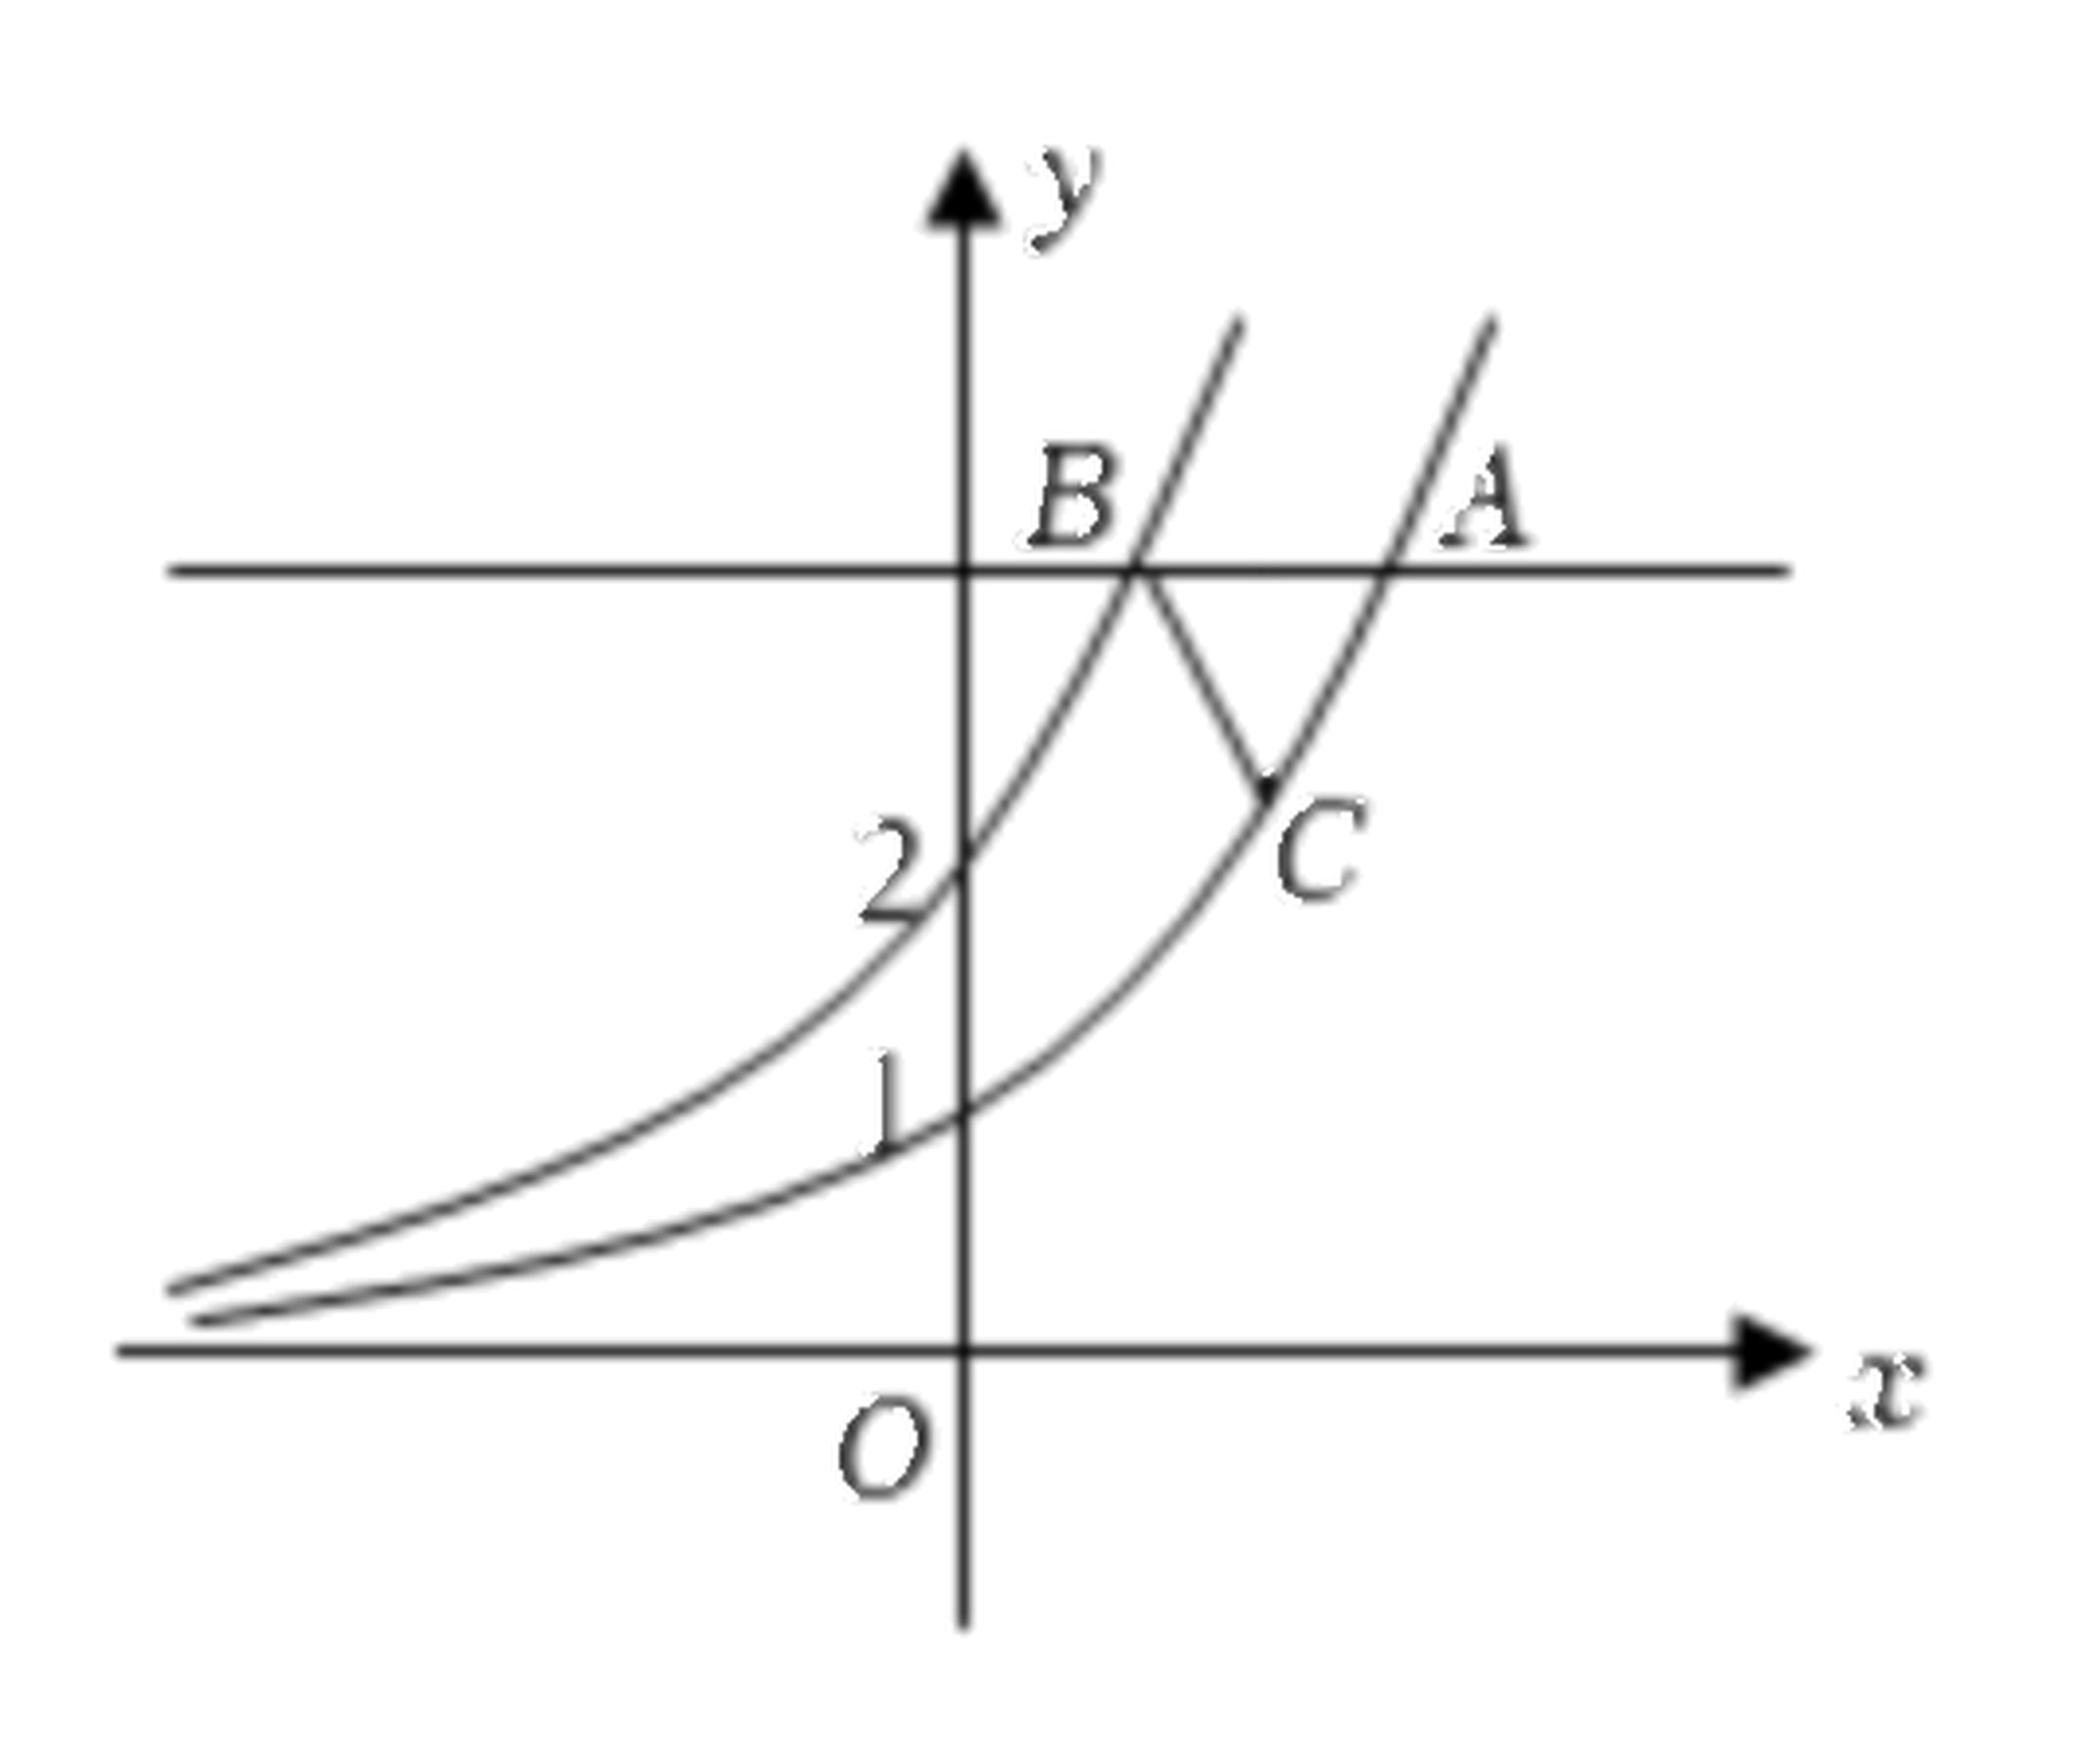
\includegraphics[width=0.40\textwidth]{figures/gao150_q11.png}
\end{center}

\ifanswer
\solbegin
\step{设直线 $l$ 的方程为 $y=a(a>0)$，}
\step{由 $2^x=a$，得 $x=\log_2 a$，所以 $A(\log_2 a,a)$，}
\step{由 $2^{x+1}=a$，得 $x=\log_2 a-1$，所以 $B(\log_2 a-1,a)$，所以 $\lvert AB\rvert=1$，}
\step{取 $AB$ 的中点 $D$，连接 $CD$，如图所示，}
\step{因为 $\triangle ABC$ 为等边三角形，则 $CD\perp AB$，且 $\lvert CD\rvert=\dfrac{\sqrt3}{2}$，}
\step{所以 $C\left(\log_2 a-\dfrac{1}{2},a-\dfrac{\sqrt3}{2}\right)$，}
\step{因为点 $C$ 在函数 $y=2^x$ 的图像上，所以 $a-\dfrac{\sqrt3}{2}=2^{\log_2 a-\frac{1}{2}}=\dfrac{a}{\sqrt2}$，}
\step{解得 $a=\dfrac{\sqrt3}{2-\sqrt2}=\dfrac{\sqrt3(2+\sqrt2)}{4-2}=\sqrt3+\dfrac{\sqrt6}{2}$，}
\step{所以点 $C$ 的纵坐标为 $a-\dfrac{\sqrt3}{2}=\dfrac{\sqrt3+\sqrt6}{2}$.}
\solend
\fi

% === Q12 === 解析配图（高斯函数方格阴影，仅答案版出）；"数学王子"弯引号；cases 块整体算一个印刷行；解析 4 行
\item 小玲在研究数学发展史，特别崇拜近代数学奠基者之一、享有“数学王子”称号的德国数学家高斯. 为了纪念高斯，我们把取整函数 $y=[x]$ 称为高斯函数，其中 $[x]$ 表示不超过 $x$ 的最大整数，如 $[1.1]=1$，$[-1.1]=-2$，则点集 $P=\{(x,y)\mid [x]^2+[y]^2=1\}$ 所表示的平面区域的面积为\blankline[4.4em].

\ifanswer
\solbegin
\step{$[x]^2+[y]^2=1$ 由 $\begin{cases}[x]=0\\ {[y]=-1}\end{cases}$ 或 $\begin{cases}[x]=0\\ {[y]=1}\end{cases}$ 或 $\begin{cases}[x]=-1\\ {[y]=0}\end{cases}$ 或 $\begin{cases}[x]=1\\ {[y]=0}\end{cases}$ 四个平面区域组成，}
\step{即 $\begin{cases}0\leqslant x<1\\ -1\leqslant y<0\end{cases}$ 或 $\begin{cases}0\leqslant x<1\\ 1\leqslant y<2\end{cases}$ 或 $\begin{cases}-1\leqslant x<0\\ 0\leqslant y<1\end{cases}$ 或 $\begin{cases}1\leqslant x<2\\ 0\leqslant y<1\end{cases}$，}
\step{作出平面区域如图所示，平面区域由四个边长为 $1$ 的正方形组成，}
\begin{center}
% 高斯函数 [x]^2+[y]^2=1 方格阴影区域图取 04 页顶部，去粉色水印、去色、4× LANCZOS 放大；仅答案版出
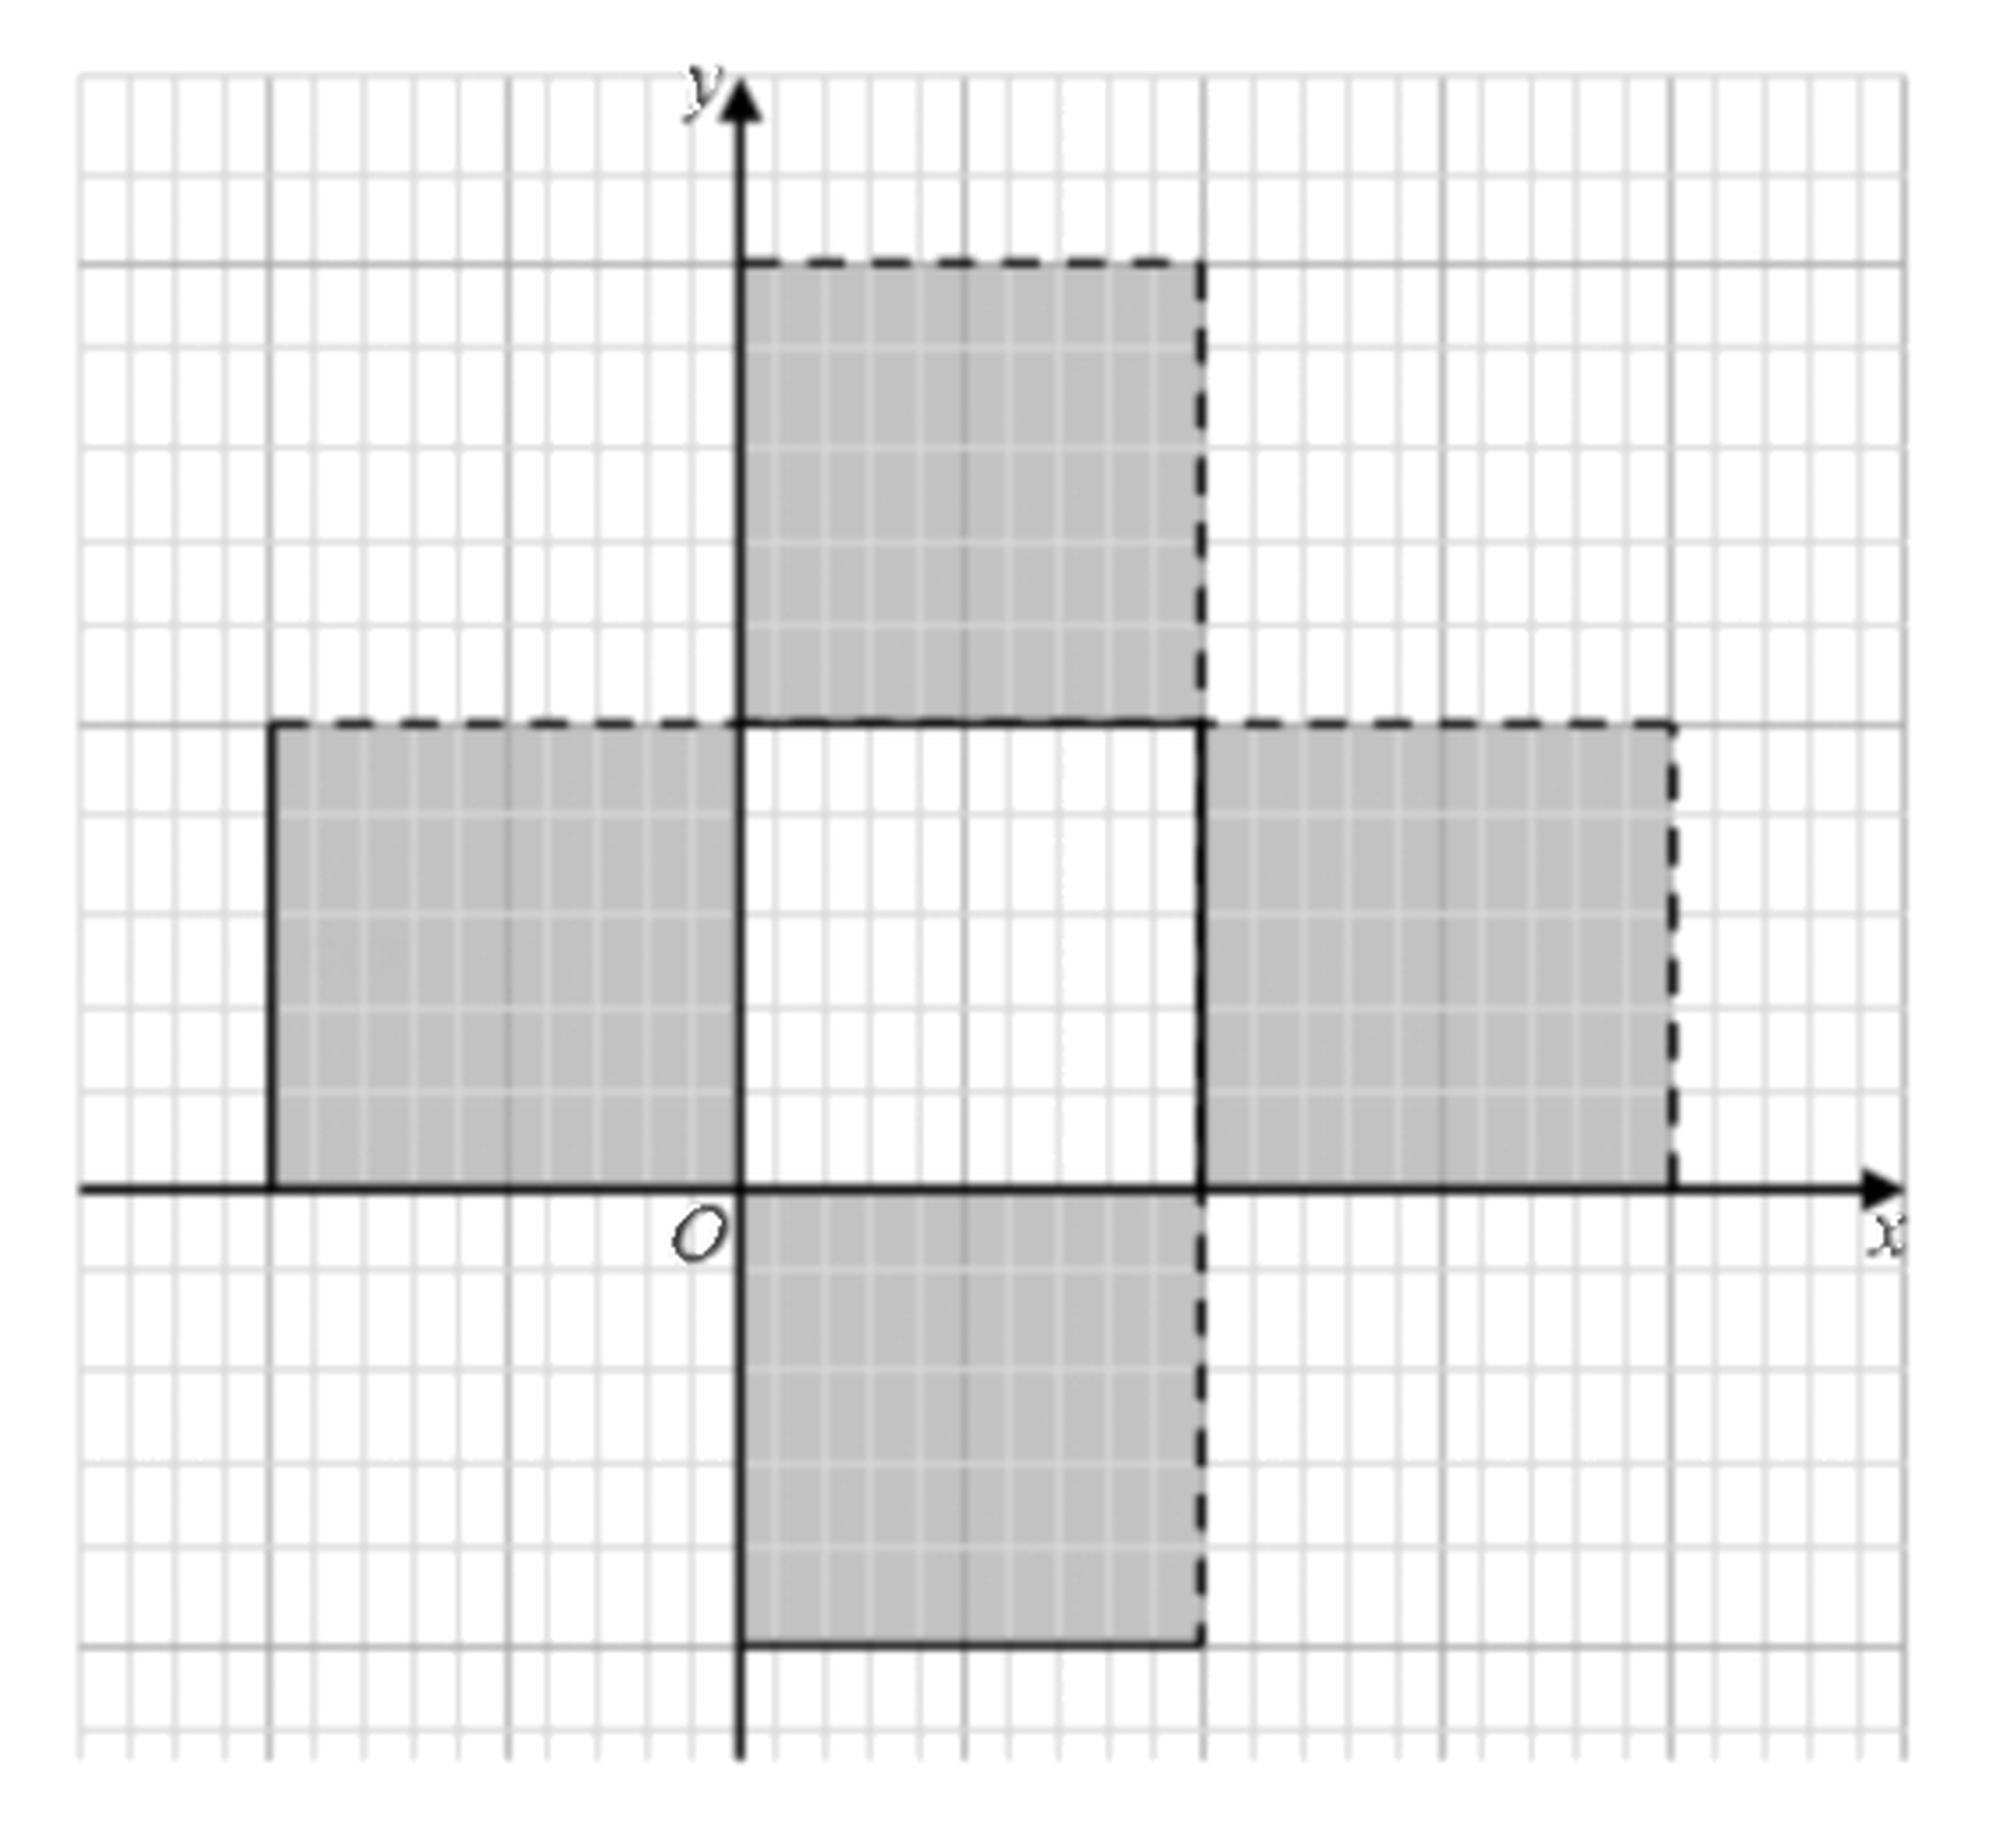
\includegraphics[width=0.34\textwidth]{figures/gao150_q12.png}
\end{center}
\step{总面积为 $1\times4=4$.}
\solend
\fi

\end{enumerate}

\bigsec{二、选择题}

\begin{enumerate}
\setcounter{enumi}{12}

% === Q13 === 答案在解析末句"故选 C"；括号 \mbox{（\quad）} 留空；四选项一行；解析 1 行
\item 设 $x\ne0$，则 $3^{\log_9 x^2}$ 的化简结果是\mbox{（\quad）}

\keepwithprev
A. $x$\qquad B. $\dfrac{1}{x}$\qquad C. $\lvert x\rvert$\qquad D. $\dfrac{1}{\lvert x\rvert}$

\ifanswer
\solbegin
\step{$3^{\log_9 x^2}=3^{\log_3\lvert x\rvert}=\lvert x\rvert$，故选 $C$.}
\solend
\fi

% === Q14 === 题目配图（两函数图像，三版都出）；\needvspace{8cm} 守卫放 \item 之前；"图像"照录；四选项两行两列；解析 2 行，故选 B
\needvspace{8cm}
\item 设 $a>0$ 且 $a\ne1$，$b\in\R$. 若函数 $y=a^{-\lvert x\rvert}$ 与 $y=x^b$ 的大致图像如图所示，则\mbox{（\quad）}

\keepwithprev
A. $0<a<1<b$\qquad\qquad B. $a>1$ 且 $b>1$

C. $0<a<1$ 且 $0<b<1$\qquad\qquad D. $0<b<1<a$

\begin{center}
% 两函数 y=a^{-|x|} 与 y=x^b 大致图像取 04 页右侧，去粉色水印、去色、4× LANCZOS 放大；三版都出
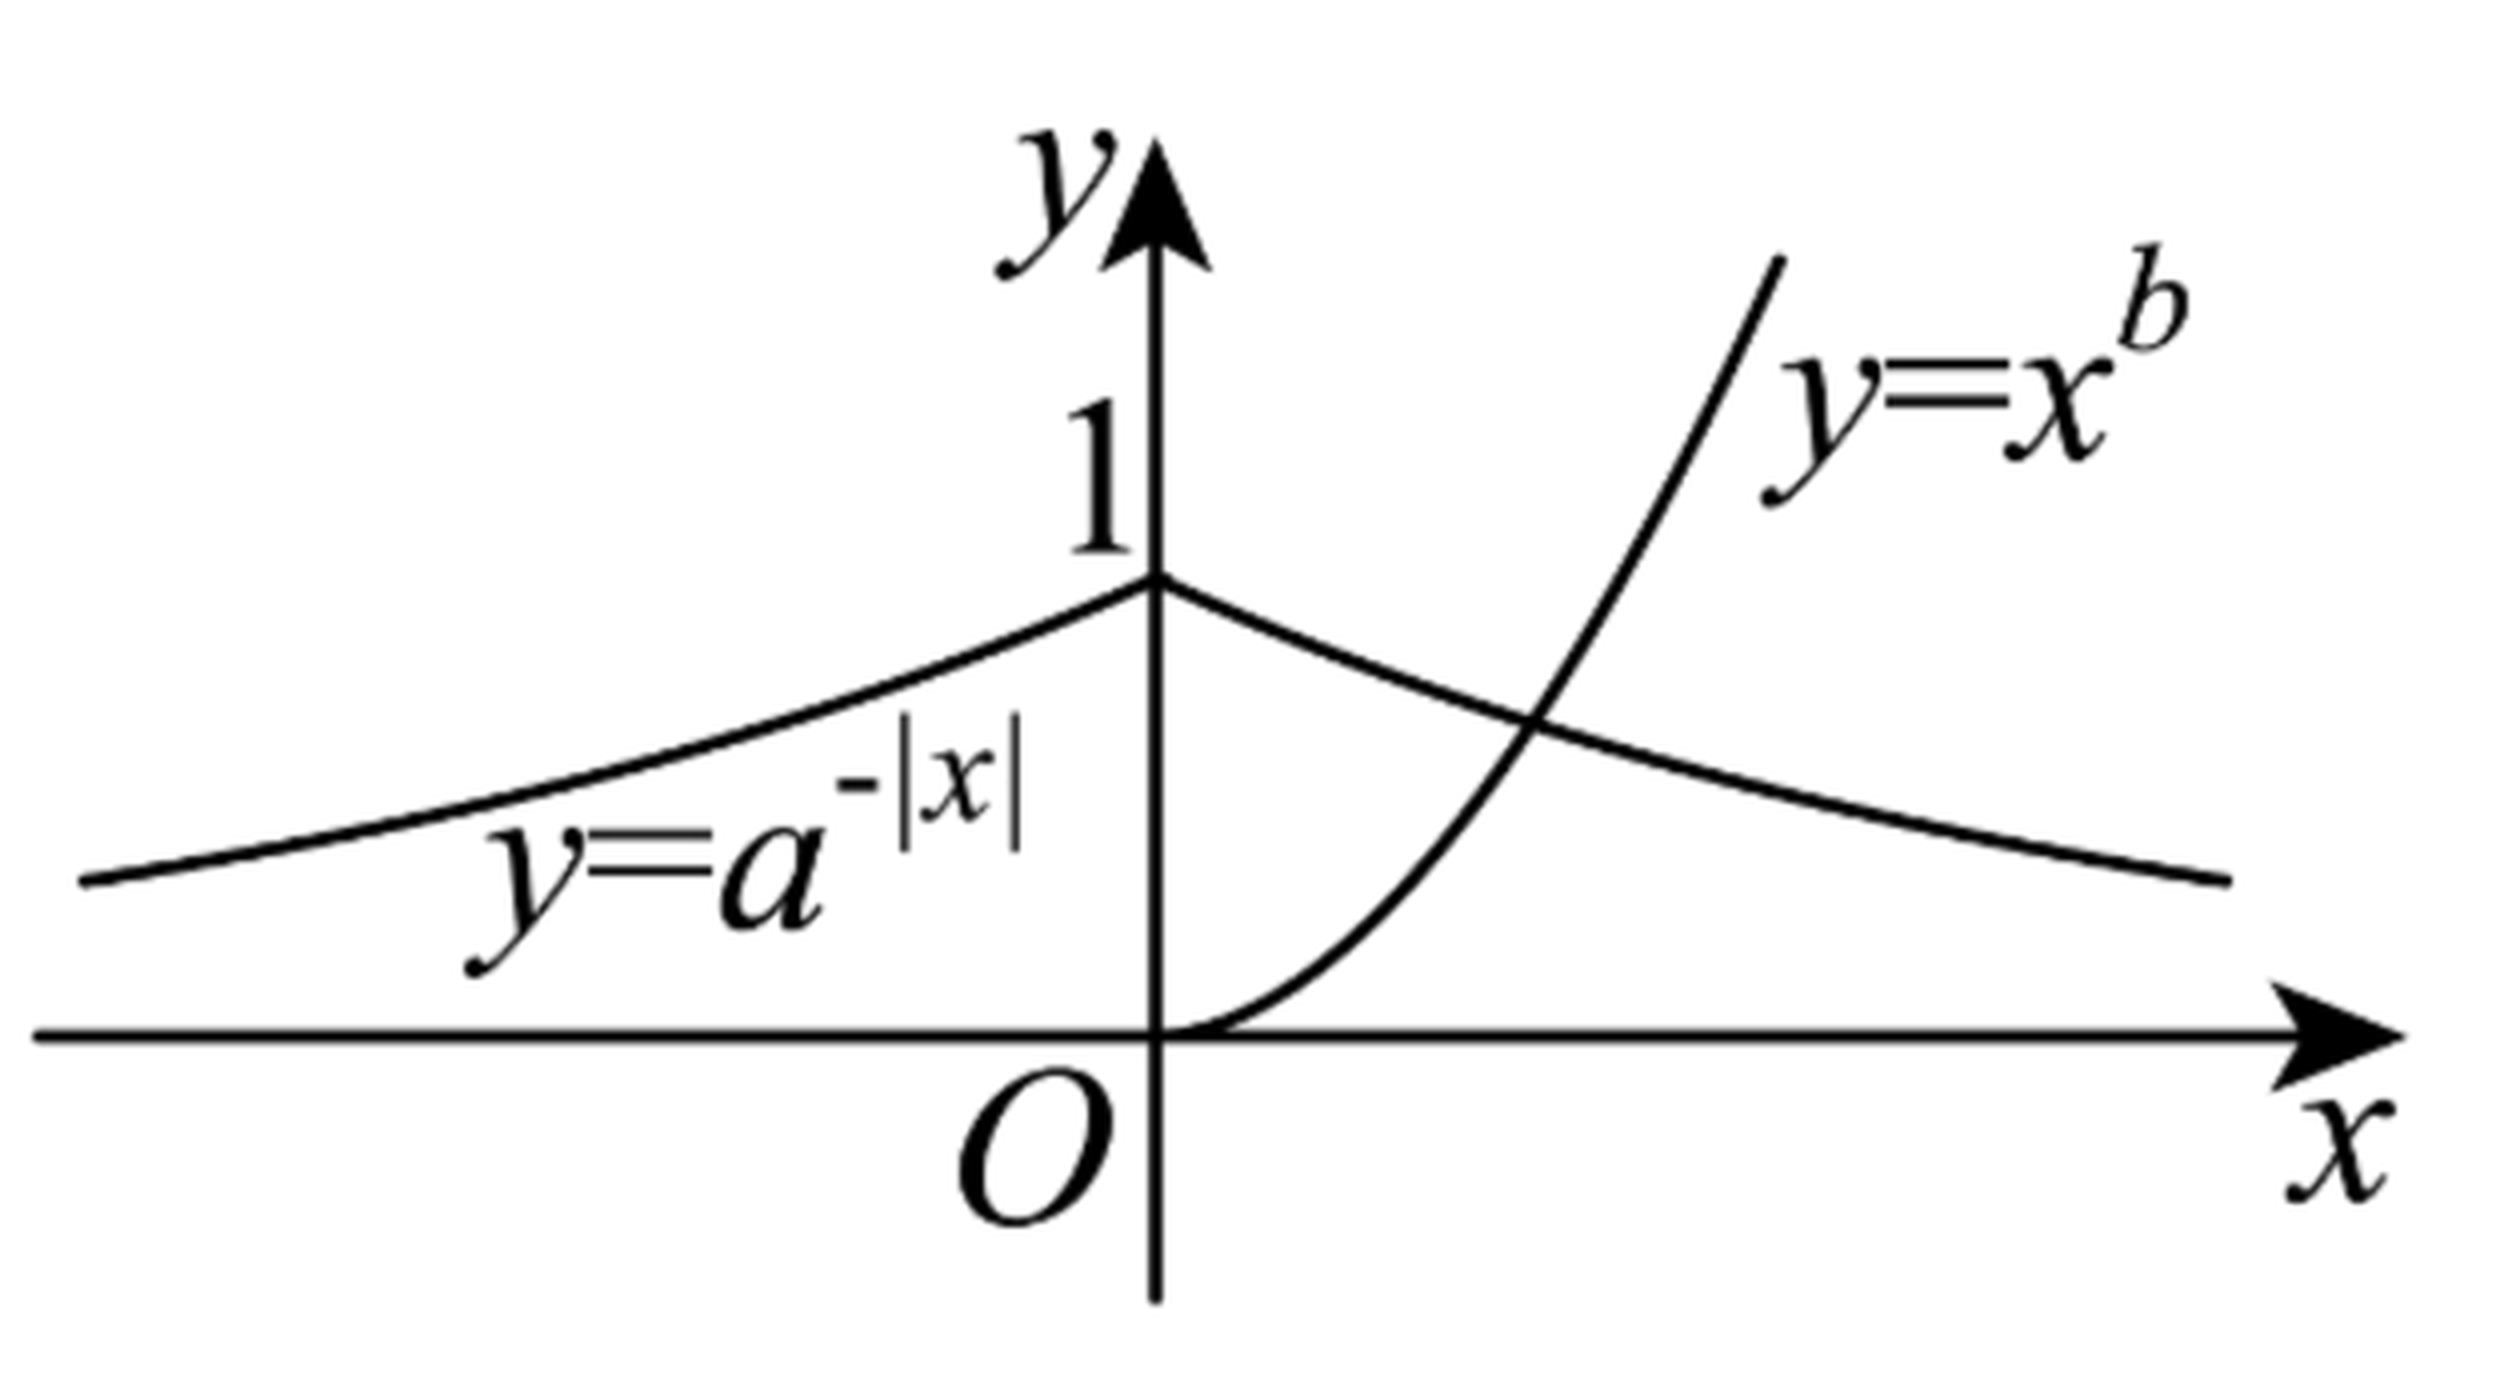
\includegraphics[width=0.40\textwidth]{figures/gao150_q14.png}
\end{center}

\ifanswer
\solbegin
\step{在 $(0,+\infty)$ 上，$y=a^{-x}$ 严格递减，得 $a>1$；}
\step{幂函数 $y=x^b$ 的图像递增且向上弯曲，得 $b>1$；故选 $B$.}
\solend
\fi

% === Q15 === "算术平均值／算术平均数"两处不同照录；四选项两行两列；解析 5 行（续 05 页顶），故选 B
\item 已知两个正数的算术平均值不小于它们的几何平均值，类比有以下结论：三个正数的算术平均数不小于它们的几何平均数，即当 $a,b,c$ 为正实数时，$\dfrac{a+b+c}{3}\geqslant\sqrt[3]{abc}$，当且仅当 $a=b=c$ 时等号成立. 利用上述结论，下列选项中判断正确的是\mbox{（\quad）}

\keepwithprev
A. 若 $x>0$，则 $2x+\dfrac{1}{x^2}\geqslant\dfrac{27}{8}$\qquad\qquad B. 若 $x>0$，则 $x^2+\dfrac{2}{x}\geqslant3$

C. 若 $0<x<1$，则 $x^2(1-x)\geqslant\dfrac{1}{9}$\qquad\qquad D. 若 $0<x<1$，则 $x^2(1-x)\leqslant\dfrac{1}{9}$

\ifanswer
\solbegin
\step{A：取 $x=1$，$2x+\dfrac{1}{x^2}=3<\dfrac{27}{8}$，错误.}
\step{B：$x^2+\dfrac{2}{x}=x^2+\dfrac{1}{x}+\dfrac{1}{x}\geqslant3\sqrt[3]{x^2\cdot\dfrac{1}{x}\cdot\dfrac{1}{x}}=3$，当且仅当 $x=1$ 时取等号，正确.}
\step{C：取 $x=\dfrac{1}{3}$，$x^2(1-x)=\dfrac{2}{27}<\dfrac{1}{9}$，错误.}
\step{D：取 $x=\dfrac{2}{3}$，$x^2(1-x)=\dfrac{4}{27}>\dfrac{1}{9}$，错误.}
\step{故选 $B$.}
\solend
\fi

% === Q16 === "完美集"新定义（弯引号、引号外空格照录）；圈数字①②文本模式；$n\in\N$；四选项两行两列；解析 9 行（6 行 05 页＋3 行 06 页顶），故选 A
\item 已知有限集 $A=\{a_1,a_2,\cdots,a_n\}$（$n\geqslant2$，$n\in\N$）. 若 $A$ 中元素 $a_i$（$i=1,2,\cdots,n$）满足 $a_1+a_2+\cdots+a_n=a_1\cdot a_2\cdots a_n$，就称 $A$ 为 “完美集”. 现有以下两个命题：

①恰有两个元素的 “完美集” 有无穷多个；

②若 $a_i$ 均为正整数，则 “完美集” $A$ 有且只有一个，且 $n=3$.

则\mbox{（\quad）}

\keepwithprev
A. ①和②都是真命题\qquad\qquad B. ①和②都是假命题

C. ①是真命题，②是假命题\qquad\qquad D. ①是假命题，②是真命题

\ifanswer
\solbegin
\step{①由 $a+b=ab\Leftrightarrow(a-1)(b-1)=1$，任取 $a>2$，则 $b=1+\dfrac{1}{a-1}\in(1,2)$，}
\step{得到无穷多个不同的完美集，①真.}
\step{②设 $1\leqslant a_1<a_2<\cdots<a_n$，则 $a_i\geqslant i$.}
\step{若 $n=2$，则 $(a_1-1)(a_2-1)=1$，只能有 $a_1=a_2=2$，与元素互异矛盾.}
\step{若 $n\geqslant4$，则 $a_1a_2\cdots a_n\geqslant a_2a_{n-1}a_n\geqslant2(n-1)a_n>na_n\geqslant a_1+\cdots+a_n$，矛盾.}
\step{当 $n=3$ 时，若 $a_1\geqslant2$，则 $a_1a_2a_3\geqslant6a_3>3a_3\geqslant a_1+a_2+a_3$，矛盾.}
\step{因此 $a_1=1$，$(a_2-1)(a_3-1)=2$，结合 $a_2<a_3$ 得 $a_2=2$，$a_3=3$.}
\step{唯一的完美集为 $\{1,2,3\}$，②真.}
\step{故选 $A$.}
\solend
\fi

\end{enumerate}

\bigsec{三、解答题}

\begin{enumerate}
\setcounter{enumi}{16}

% === Q17 === \varnothing 空集、$B\subseteq A$ 带下划线照录；弯引号内空格照录；解析 7 行
\item 设 $a,b\in\R$. 已知集合 $A=\{x\mid ax^2+3x-a>3\}$，$B=\{x\mid bx=1\}$.

(1) 若 $A=(1,2)$，求 $a$ 的值；

(2) 若 $a=0$，且 “ $x\in A$ ” 是 “ $x\in B$ ” 的必要非充分条件，求 $b$ 的取值范围.

\ifanswer
\solbegin
\step{(1) $A=(1,2)$，则 $a<0$，且 $1,2$ 是方程 $ax^2+3x-a-3=0$ 的两根.}
\step{由 $4a+6-a-3=0$，得 $a=-1$，此时不等式为 $-(x-1)(x-2)>0$，}
\step{解集确为 $(1,2)$.}
\step{(2) $a=0$ 时，$A=(1,+\infty)$，题意等价于 $B\subseteq A$ 且 $B\ne A$.}
\step{当 $b=0$ 时，$B=\varnothing$，符合条件.}
\step{当 $b\ne0$ 时，$B=\left\{\dfrac{1}{b}\right\}$，条件等价于 $\dfrac{1}{b}>1$，解得 $0<b<1$.}
\step{因此 $b$ 的取值范围为 $[0,1)$.}
\solend
\fi

% === Q18 === $p\in\Z$；"图像"（像，有亻）照录；指数 $-2p^2+5p$；解析 8 行（(1) 首行 06 页末＋2 行 07 页顶、(2) 5 行 07 页）
\item 设 $p\in\Z$，已知 $f(x)=x^{-2p^2+5p}$.

(1) 若幂函数 $y=f(x)$ 的图像关于原点成中心对称，且满足 $f(3)<f(4)$，求 $p$ 的值；

(2) 当 $p=-2$ 时，求满足 $f(2x+3)<f(x-4)$ 的 $x$ 的取值范围.

\ifanswer
\solbegin
\step{(1) 图像关于原点成中心对称，得整数 $-2p^2+5p$ 为奇数.}
\step{由 $f(3)<f(4)$，得 $-2p^2+5p>0\Leftrightarrow0<p<\dfrac{5}{2}$，}
\step{结合 $p\in\Z$，得 $p=1$ 或 $p=2$，对应指数分别为 $3$、$2$，所以 $p=1$.}
\step{(2) 当 $p=-2$ 时，$f(x)=\dfrac{1}{x^{18}}$，定义域为 $\{x\in\R\mid x\ne0\}$.}
\step{原不等式要求 $x\ne-\dfrac{3}{2}$ 且 $x\ne4$，}
\step{此时 $\dfrac{1}{(2x+3)^{18}}<\dfrac{1}{(x-4)^{18}}\Leftrightarrow\lvert 2x+3\rvert>\lvert x-4\rvert\Leftrightarrow(2x+3)^2>(x-4)^2$，}
\step{因此 $(x+7)(3x-1)>0\Leftrightarrow x<-7$ 或 $x>\dfrac{1}{3}$，}
\step{排除 $x=4$，得 $x\in(-\infty,-7)\cup\left(\dfrac{1}{3},4\right)\cup(4,+\infty)$.}
\solend
\fi

% === Q19 === $a\in\R$、$g(x)=f(2x+1)+a\cdot f(x)+2$；解析 6 行（(2) 末两行续 08 页顶）
\item 已知 $f(x)=2^x$.

(1) 求方程 $f(2x)-f(x)=6$ 的解；

(2) 设 $a\in\R$，$g(x)=f(2x+1)+a\cdot f(x)+2$，若对于任意 $x\in[-1,1]$，均有 $g(x)\geqslant1$，求 $a$ 的取值范围.

\ifanswer
\solbegin
\step{(1) 令 $t=2^x>0$，则 $t^2-t-6=(t-3)(t+2)=0$，}
\step{由 $t>0$ 得 $t=3$，所以 $x=\log_2 3$.}
\step{(2) 令 $t=2^x$，则 $t\in\left[\dfrac{1}{2},2\right]$，且 $g(x)\geqslant1\Leftrightarrow2t^2+at+1\geqslant0\Leftrightarrow a\geqslant-\left(2t+\dfrac{1}{t}\right)$，}
\step{由基本不等式得 $2t+\dfrac{1}{t}\geqslant2\sqrt{2t\cdot\dfrac{1}{t}}=2\sqrt2$，}
\step{当且仅当 $t=\dfrac{1}{\sqrt2}\in\left[\dfrac{1}{2},2\right]$ 时等号成立，}
\step{因此 $-\left(2t+\dfrac{1}{t}\right)$ 的最大值为 $-2\sqrt2$，所求范围为 $a\in[-2\sqrt2,+\infty)$.}
\solend
\fi

% === Q20 === "极闭集"新定义、3 问，全卷末题；$M\subseteq(0,+\infty)$ 带下划线照录；自定义运算 $x*y$ 星号照录；解析 13 行（9 行 08 页＋4 行 09 页上半）
\item 对于非空实数集 $M\subseteq(0,+\infty)$，若满足以下两个条件：

① $M$ 中至少含有 $2$ 个元素，且 $1\notin M$；

②对于 $M$ 中任意两个不相等的元素 $x$、$y$，定义 $x*y=\dfrac{xy+1}{x+y}$，且 $x*y\in M$.

则称 $M$ 为 “极闭集”.

(1) 分别判断集合 $A=\left\{\dfrac{1}{2},3\right\}$ 与集合 $B=(1,+\infty)$ 是否为 “极闭集” （无需理由）；

(2) 若 $M$ 是 “极闭集”，证明：$M$ 中不可能所有元素都小于 $1$；

(3) 证明：不存在任何有限集是 “极闭集”.

\ifanswer
\solbegin
\step{(1) $A$ 不是 “极闭集”，$B$ 是 “极闭集”.}
\step{(2) 假设 $M$ 中所有元素都小于 $1$，取其中两个不相等的元素 $x$、$y$，}
\step{则 $x*y-1=\dfrac{(1-x)(1-y)}{x+y}>0$，}
\step{这与 $x*y\in M$ 且 $M$ 中所有元素都小于 $1$ 矛盾.}
\step{(3) 假设有限集 $M$ 是 “极闭集”，}
\step{由 (2) 及 $1\notin M$，得 $M$ 中存在大于 $1$ 的元素.}
\step{若 $M$ 中有小于 $1$ 的元素，取其中最大的一个为 $a$，另取 $b\in M$ 且 $b>1$，}
\step{则 $a*b-a=\dfrac{1-a^2}{a+b}>0, a*b-1=\dfrac{(a-1)(b-1)}{a+b}<0$，}% 半角逗号在两个数学式组之间，全稿惯例、非笔误，照录
\step{于是 $a<a*b<1$ 且 $a*b\in M$，与 $a$ 的最大性矛盾.}
\step{若 $M$ 中没有小于 $1$ 的元素，则 $M\subseteq(1,+\infty)$.}
\step{取 $a=\min M$，另取 $b\in M$ 且 $b\ne a$，则 $a*b-a=\dfrac{1-a^2}{a+b}<0$，}
\step{于是 $a*b<a$ 且 $a*b\in M$，与 $a$ 的最小性矛盾.}
\step{因此不存在任何有限集是 “极闭集”.}
\solend
\fi

\end{enumerate}

\end{document}
"
%
% ① 原始材料：微信公众号"魔都数学加油站"文章，连载"27学年高一150"，原文标题
% "27学年高一150——2026-2027年上海市曹杨二中高一上期中"；
% 原文链接：https://mp.weixin.qq.com/s/xlQxmik8TZXR87RC6MnCrw 。
% 正文为 9 张 PNG 页（01/02/04/06/07/09 为 2560×3620，03/05/08 为 4762×6735，
% 同一篇各页分辨率混排，逐页按各自分辨率裁图核对，别按预览比例换算裁框）。
% 体例：讲评版——全 18 题均印【解析】（逐题核实，见 ② ②）。
% 题目、答案、解析均据原图转录；卷面粉红色/红色水印"魔都数学加油站"及公众号页脚未录入。
% 全卷插图清单（逐页通读 9 页确认）：3 幅——
%   · Q11 题目配图（指数函数曲线图，02 页右侧：x/y 轴、O、y=2^x 与 y=2^{x+1}
%     两曲线、A/B/C 三点、刻度 1/2、等边三角形 ABC），三版都出，裁 figures/gao150_q11.png；
%   · Q12 解析配图（高斯函数取整 [x]^2+[y]^2=1 方格阴影区域图，04 页顶部：4 个边长 1
%     的正方形组成的十字形阴影），解析"作出平面区域如图所示"处，仅答案版出，
%     放 \ifanswer 内 \step 之间，裁 figures/gao150_q12.png；
%   · Q14 题目配图（两函数 y=a^{-|x|} 与 y=x^b 大致图像，04 页右侧：x/y 轴、O、
%     y 轴刻度 1、一递减曲线一递增上翘曲线），三版都出，裁 figures/gao150_q14.png；
%   其余各页逐页确认无其它题目配图、无表格；Q11/Q12 解析"如图所示"对应的就是上列
%   已裁的图，不重复裁；09 页上半为 Q20(3) 解析续尾、下半仅水印、无正文。
%   3 图均取自原卷截图，去粉色水印、去色、4× LANCZOS 放大。
%
% 卷首标题：原卷印作"2026-2027 年曹杨二中高一上期中"，年份区间按全稿惯例排 en dash；
% 原卷卷面未印副标题，本稿按同期中卷知识模块口径补出"集合与常用逻辑用语、不等式、函数"。
%
% 题号体例（逐页核实定稿）：本卷共 18 题——一、填空题 3—12（10 题）、
% 二、选择题 13—16（4 题）、三、解答题 17—20（4 题）。
% 三节分别 \setcounter{enumi}{2}／{12}／{16}。原卷从第 3 题起、无第 1、2 题，
% 本稿保留原题号；全卷末题为第 20 题（"极闭集"新定义、3 问），无 Q21、无附加题节。
%
% ② 与原卷的排版差异：
%   ① 原文从第 3 题起，本稿保留原题号；共 18 题三节，解答题只有 4 题到 20；
%   ② 全 18 题均印【解析】，用 \solbegin…\solend；逐题核实无只印【答案】或
%      答案印题干括号内的题；四道选择题答案在解析末句"故选 X"（Q13 选 C、
%      Q14 选 B、Q15 选 B、Q16 选 A，逐个放大复核）、括号 \mbox{（\quad）} 留空、
%      不另提 \ans{}；答案版【答案】/【解析】标记数 = 18 = 全卷题数；
%   ③ 原卷卷面未印副标题，本稿按知识模块口径补出；
%   ④ 原卷填空横线按全稿惯例排 \blankline[4.4em]；选择题括号排 \mbox{（\quad）}、
%      选项段前按惯例加 \keepwithprev；解答题不留作答区、不加 \anspace（原卷为讲评版）；
%   ⑤ 数集黑板粗体：Q4"m\in R"、Q5"a,b\in R"、Q6"a,b,c\in R"、Q7"a\in R"、
%      Q10"a\in R"、Q14"b\in R"、Q17"a,b\in R"、Q18"p\in Z"／定义域"x\in R"、
%      Q19"a\in R"、Q16"n\in N" 原卷印斜体 R/Z/N，按全稿惯例归一 \R／\Z／\N；
%      绝对值排 \lvert…\rvert（Q7 |x+4|+|x-3|、Q11 |AB|／|CD|、Q13 |x|、
%      Q18 |2x+3|／|x-4|），集合描述竖线排 \mid（Q3、Q12、Q17、Q18、Q20），
%      不等号按全稿惯例排 \leqslant／\geqslant；补集照原卷上划线排 \overline{A}
%      （Q3 题干＋解析共 2 处）；空集符号 \varnothing（Q17 解析(2)）；
%      子集 \subset（单线⊂）／\subseteq（带下划线⊆）逐处照录，本卷 3 处子集
%      符号均印带下划线 ⊆、照录 \subseteq（Q20 题干、Q20 解析(3)、Q17 解析(2)，
%      见 ④），无 \subset 用例；
%   ⑥ 判别式 Δ/△：逐页通读 9 页，本卷无一元二次判别式算式，故无 Δ/△ 混用可照录
%      （"高 \Delta／扁 \triangle"口径备查，参照 高一142／144／145／146／148／149
%      头注④）；本卷仅 Q11 题干与解析共 2 处几何三角形符号 △ABC，逐处放大并排
%      确认两处同形、印近等边粗线三角（非判别式），照录 \triangle（见 ④）；
%   ⑦ 中文弯引号照录：Q12"数学王子"、Q16"完美集"（题干＋①②两命题，引号外
%      留空格）、Q17" x∈A "" x∈B "（引号内空格）、Q20"极闭集"（题干条件、
%      三问与解析，引号外留空格）；注释里一律 ASCII 引号；数学式内 CJK 用 \text{}
%      （Q3 集合描述"且"用 \text{ 且 }）；
%   ⑧ 半角逗号在数学组之间是全稿惯例、非笔误，逐处照录（Q17 解析"1,2 是方程…
%      两根"、Q20 解析(3)">0, a*b-1=…<0" 两式之间等）；行末西文句点 ASCII `.`；
%      行中全角逗号／顿号照录（Q12"之一、享有"、Q18 解析"3、2"、Q20"x、y"）；
%   ⑨ "图像／图象"逐处放大核：全卷 9 处均印"图像"（像，有亻）、未见"图象"——
%      Q4 题干 1、Q11 题干 2＋解析 1、Q14 题干 1＋解析 1、Q18 题干 1＋解析 1；
%      同卷"第二象限""象限"用"象"（无亻）。逐处照录未统一改动（放大 01/02/04/06
%      页 /tmp/gao150/z/p01_q4_tuxiang2.png、p04_q14_tuxiang2.png、
%      p02_q11_lines.png 确认）；子题标号 (1)(2)(3) 半角括号照录；圈数字①②
%      在文本模式（Q16 两命题与解析、Q20 两条件与三问及解析）按 common.sty
%      划入 CJK 字符类渲染，进数学式用 \text{①}；
%   ⑩ Q20 新定义 x*y=\dfrac{xy+1}{x+y} 的 * 是自定义运算（星号），照录；
%      \left…\right 不得拆到不同 $…$ 组（Q19"\left(2t+\frac1t\right)"、
%      Q20 题干"A=\left\{\frac12,3\right\}"等）；Q8 嵌套根号
%      \sqrt{\frac2x+\frac{16}{1-2x}}、Q9 对数连加 \log_2 A 等复杂式照录别简化；
%   ⑪ 一条 \step = 原卷解析的一个印刷行，cases 块整体算一个印刷行；别并折行、
%      别拆行。Q4 三行、Q8 五行、Q11 九行、Q12 四行（两行各含四个 cases 块）、
%      Q15 五行、Q16 九行、Q18 八行、Q20 十三行均按印刷行逐条断，不丢行；
%   ⑫ 配图：Q11／Q14 题目配图（三版都出）放 \item 内题干之后 \begin{center}，
%      大图块加 \needvspace{8cm} 守卫把整块推走（守卫放 \item 之前，见
%      高一145 Q14/Q20 成例与切页审计 B 类坑）；Q12 解析配图（仅答案版出）
%      放 \ifanswer 内 \solbegin…\solend 的 \step 之间（高一73 第16题成例）；
%   ⑬ 跨页续印按题合并：见 ⑥；
%   ⑭ 原卷解析内无红色"法一／法二"之类小标题，故本卷无 \stepm；红色水印
%      "魔都数学加油站"不录入；Q12 解析"作出平面区域如图所示"对应的图即
%      ① 所列 gao150_q12.png（04 页顶部），不重复裁；Q11 解析"如图所示"对应
%      题目配图 gao150_q11.png，不另裁。
%
% ③ 行数复核：一条 \step／\stepm = 原卷解析的一个印刷行，cases 块作一个印刷行计。
%   逐题数（主会话逐页核对定稿）：Q3：1；Q4：3；Q5：2；Q6：1；Q7：2；Q8：5；
%   Q9：1；Q10：3；Q11：9；Q12：4；Q13：1；Q14：2；Q15：5；Q16：9；
%   Q17：7；Q18：8；Q19：6；Q20：13。
%   合计 82 条 \step（本卷无 \stepm：解析内无红色"法一／法二"类小标题），
%   与原卷逐题印刷行相等。全卷 18 题均设 \solbegin…\solend，答案版
%   【答案】/【解析】标记数 = 18 = 全卷题数。
%
% ④ 判别式／三角形／子集符号结论（逐处放大原图照录、不得统一，主会话像素级复核）：
%   判别式：逐页通读 9 页，本卷无一元二次判别式 Δ/△ 算式（Q18 讨论幂函数指数
%     奇偶、不用判别式；Q9／Q19／Q20 亦无），头注 ② ⑥ 的"高 \Delta／扁 \triangle"
%     口径在本卷无对应处（参照 高一142／144／145／146／148／149 头注④，仅备查）。
%   几何三角形符号：Q11 题干"使得 △ABC 为等边三角形"（02 页末）与解析
%     "因为 △ABC 为等边三角形，则 CD⊥AB"（03 页）共 2 处，放大 02/03 页
%     /tmp/gao150/z/q11_tri_montage2.png 并排确认两处同形、印近等边粗线三角
%     （h/w≈0.98、非"高>宽"的判别式 \Delta），照录 \triangle（与 高一105
%     "使得 \triangle ABC 为等边三角形" 同短语成例、高一149 几何三角形照录
%     \triangle 口径一致），不引入 \Delta。
%   子集／补集：Q20 题干"$M\subseteq(0,+\infty)$"（08 页）、Q20 解析(3)
%     "则 $M\subseteq(1,+\infty)$"（09 页）、Q17 解析(2)"题意等价于 $B\subseteq A$
%     且 $B\ne A$"（06 页）共 3 处子集符号，逐处放大（/tmp/gao150/z/p08_q20_stem.png、
%     p09_q20_sub.png、p06_q17_sub.png）确认均印带下划线 ⊆，照录 \subseteq；
%     本卷未见单线 ⊂（\subset）之对应处。Q3 题干与解析共 2 处补集照原卷上划线
%     排 \overline{A}；Q17 解析(2) 空集印 ∅、照录 \varnothing（Q7"解集为空集"
%     为中文词、非符号，照录文字）；集合描述竖线 \mid；数集 \R／\Z／\N 归一见 ② ⑤。
%
% ⑤ 存疑照录（放大原图确认，照录未改、正文对应处另有 % 注）：
%   1. Q8 解析第 4 行"所以 $y=\frac1x+\frac{8}{1-2x}$ 的最小值为 18" —— 上文
%      并未定义 $y$，且题面求的是 $\sqrt{\frac2x+\frac{16}{1-2x}}$ 的最小值；
%      按上下文该行应为 $\frac1x+\frac{8}{1-2x}$ 的最小值为 18（$y$ 疑为原卷
%      衍字／笔误），放大 02 页 /tmp/gao150/z/p02_q8_y.png 确认，照录未改。
%   2. Q20 解析(3)"$a*b-a=\frac{1-a^2}{a+b}>0, a*b-1=\frac{(a-1)(b-1)}{a+b}<0$"
%      两式之间的逗号原卷印半角 ,（非全角），按全稿惯例"半角逗号在数学组之间"
%      照录未改（放大 08 页 /tmp/gao150/z/p08_q20_sol8.png 确认）。
%   3. Q15 题干"两个正数的算术平均值…几何平均值"与"三个正数的算术平均数…
%      几何平均数"两处"值／数"用字不同，逐处照录未统一（放大 04 页确认）。
%   4. "图像／图象"全卷 9 处均印"图像"（像，有亻）、未见"图象"，逐处放大核实
%      照录、未统一改动（见 ② ⑨）；本卷判别式 Δ/△ 无用例、几何三角形 2 处
%      照录 \triangle（见 ④）。
%   全卷除此 4 类外未发现其它笔误／自相矛盾处；18 题均印【解析】、无只印【答案】
%   或答案印题干括号内的题（见 ② ②）。
%
% ⑥ 跨页续印按题合并说明（逐页核实定稿）：Q3/4/5/6/7 题干＋解析在 01 页；
%   Q8 题干＋解析 5 行、Q9 题干＋解析 1 行在 02 页上半；Q10 题干＋解析 3 行
%   在 02 页下半；Q11 题干（前两行）＋配图在 02 页下半、题干续"三角形，则点 C
%   的纵坐标为___"与解析 9 行全在 03 页上半（解析"如图所示"对应题目配图）；
%   Q12 题干＋解析 4 行在 03 页下半，解析配图（方格阴影）续印在 04 页顶部；
%   "二、选择题"标题在 04 页中部；Q13 题干＋选项＋解析、Q14 题干＋选项＋
%   配图＋解析在 04 页；Q15 题干＋四选项在 04 页末、解析 5 行续 05 页上半；
%   Q16 题干＋①②两命题＋"则(  )"＋四选项＋解析前 6 行在 05 页、解析末 3 行
%   （"因此 a_1=1…②真""故选 A"）续 06 页顶部；"三、解答题"标题在 06 页；
%   Q17 题干(1)(2)＋解析(1) 3 行＋解析(2) 首行在 06 页、解析(2) 续 3 行
%   在 06 页下半；Q18 题干(1)(2)＋解析(1) 首行在 06 页末、解析(1) 续 2 行＋
%   解析(2) 5 行在 07 页上半；Q19 题干(1)(2)＋解析(1) 2 行＋解析(2) 前 2 行
%   在 07 页下半、解析(2) 末 2 行续 08 页顶部；Q20 题干（新定义＋①②两条件）
%   ＋三问＋解析(1)(2)(3) 前 9 行在 08 页、解析(3) 末 4 行续 09 页上半，
%   末行"因此不存在任何有限集是极闭集"为全卷收尾（09 页下半仅水印、无正文）。
%   本稿按题连排，不丢行、不并折行；全卷末题为第 20 题，无 Q21、无附加题节。
%
\documentclass[a4paper,11pt]{article}
\usepackage{common}

\begin{document}

\examtitlest[3]{2026--2027 年曹杨二中高一上期中}{集合与常用逻辑用语、不等式、函数}

\bigsec{一、填空题}

\begin{enumerate}
\setcounter{enumi}{2}

% === Q3 === 补集上划线 \overline{A}（题干＋解析各 1 处）；集合描述竖线 \mid、数学式内"且"用 \text{}；解析 1 行
\item 设全集 $U=\{1,2,3,4,5\}$，集合 $A=\{x\mid x^2-3x\leqslant0\text{ 且 }x\in U\}$，则 $\overline{A}=$\blankline[4.4em].

\ifanswer
\solbegin
\step{$x^2-3x\leqslant0\Leftrightarrow0\leqslant x\leqslant3$，所以 $A=\{1,2,3\}$，$\overline{A}=\{4,5\}$.}
\solend
\fi

% === Q4 === "图像"（像，有亻）逐处照录、同句"第二象限"用"象"（无亻）；解析 3 行
\item 设 $m\in\R$. 若幂函数 $y=(m^2-5m+1)x^{m+1}$ 的图像经过第二象限，则 $m=$\blankline[4.4em].

\ifanswer
\solbegin
\step{幂函数的系数为 1，故 $m^2-5m+1=1\Rightarrow m=0$ 或 $m=5$.}
\step{$m=0$ 时，$y=x$ 不经过第二象限；}
\step{$m=5$ 时，$y=x^6$ 经过第二象限，因此 $m=5$.}
\solend
\fi

% === Q5 === 解析 2 行
\item 设 $a,b\in\R$. 若 $a^2+\dfrac{b^2}{4}=1$，则 $ab$ 的最大值为\blankline[4.4em].

\ifanswer
\solbegin
\step{$1-ab=\left(a-\dfrac{b}{2}\right)^2\geqslant0$，即 $ab\leqslant1$；}
\step{当 $a=\dfrac{\sqrt2}{2}$，$b=\sqrt2$ 时取等号，最大值为 1.}
\solend
\fi

% === Q6 === 解析 1 行
\item 设 $a,b,c\in\R$. 若等式 $2x^2-3x-2=a(x-1)^2+b(x-1)+c$ 恒成立，则 $a-b+c=$\blankline[4.4em].

\ifanswer
\solbegin
\step{令 $x=0$，得 $a-b+c=-2$.}
\solend
\fi

% === Q7 === 绝对值 \lvert…\rvert；解析 2 行
\item 设 $a\in\R$. 若关于 $x$ 的不等式 $\lvert x+4\rvert+\lvert x-3\rvert<a$ 的解集为空集，则 $a$ 的取值范围是\blankline[4.4em].

\ifanswer
\solbegin
\step{$\lvert x+4\rvert+\lvert x-3\rvert\geqslant\lvert(x+4)-(x-3)\rvert=7$，当 $-4\leqslant x\leqslant3$ 时取等号.}
\step{原不等式的解集为空集当且仅当 $a\leqslant7$，即 $a\in(-\infty,7]$.}
\solend
\fi

% === Q8 === 嵌套根号 \sqrt{\frac{2}{x}+\frac{16}{1-2x}} 照录别简化；解析 5 行
\item 设 $x\in\left(0,\dfrac{1}{2}\right)$，则 $\sqrt{\dfrac{2}{x}+\dfrac{16}{1-2x}}$ 的最小值为\blankline[4.4em].

\ifanswer
\solbegin
\step{因为 $x\in\left(0,\dfrac{1}{2}\right)$，所以 $1-2x>0$，又 $2x+1-2x=1$，}
\step{所以 $\left(\dfrac{1}{x}+\dfrac{8}{1-2x}\right)(2x+1-2x)=10+\dfrac{1-2x}{x}+\dfrac{16x}{1-2x}$}
\step{$\geqslant10+2\sqrt{\dfrac{1-2x}{x}\cdot\dfrac{16x}{1-2x}}=18$，}
\step{当且仅当 $\dfrac{1-2x}{x}=\dfrac{16x}{1-2x}$ 即 $x=\dfrac{1}{6}$ 时取等号，所以 $y=\dfrac{1}{x}+\dfrac{8}{1-2x}$ 的最小值为 18，}% 原卷此处径写 $y=\frac1x+\frac{8}{1-2x}$（上文未定义 $y$、且与题面根式不符），疑笔误，放大 02 页确认，照录未改（见 ⑤）
\step{所以 $\sqrt{\dfrac{2}{x}+\dfrac{16}{1-2x}}$ 的最小值为 6.}
\solend
\fi

% === Q9 === 对数连加 \log_2 A 等复杂式照录别简化；解析 1 行
\item 记 $A=1\times2\times3\times\cdots\times2026$，则 $\dfrac{1}{\log_2 A}+\dfrac{1}{\log_3 A}+\dfrac{1}{\log_4 A}+\cdots+\dfrac{1}{\log_{2026}A}=$\blankline[4.4em].

\ifanswer
\solbegin
\step{原式 $=\log_A 2+\cdots+\log_A 2026=\log_A(2\times3\times\cdots\times2026)=\log_A A=1$.}
\solend
\fi

% === Q10 === "严格减函数／不恒为负／⇔"照录；解析 3 行
\item 设 $a\in\R$，$f(x)=\dfrac{ax+1}{x+2}$. 若函数 $y=f(x)$ 在 $[1,+\infty)$ 上是严格减函数，且在 $[1,+\infty)$ 上的函数值不恒为负，则 $a$ 的取值范围是\blankline[4.4em].

\ifanswer
\solbegin
\step{当 $1\leqslant x_1<x_2$ 时，$f(x_2)-f(x_1)=\dfrac{(2a-1)(x_2-x_1)}{(x_1+2)(x_2+2)}$，故严格递减 $\Leftrightarrow a<\dfrac{1}{2}$.}
\step{此时最大函数值为 $f(1)$，函数值不恒为负 $\Leftrightarrow f(1)=\dfrac{a+1}{3}\geqslant0\Leftrightarrow a\geqslant-1$，}
\step{得 $a\in\left[-1,\dfrac{1}{2}\right)$.}
\solend
\fi

% === Q11 === 题目配图（指数函数曲线，三版都出）；\needvspace{8cm} 守卫放 \item 之前；"图像"照录、几何三角形 \triangle；解析 9 行（全在 03 页）
\needvspace{8cm}
\item 如图，点 $C$ 是函数 $y=2^x$ 的图像上的一点，若存在平行于 $x$ 轴的直线 $l$ 分别与函数 $y=2^x$ 和 $y=2^{x+1}$ 的图像相交于点 $A$、$B$，使得 $\triangle ABC$ 为等边三角形，则点 $C$ 的纵坐标为\blankline[4.4em].

\begin{center}
% 指数函数曲线图取 02 页右侧，去粉色水印、去色、4× LANCZOS 放大；三版都出
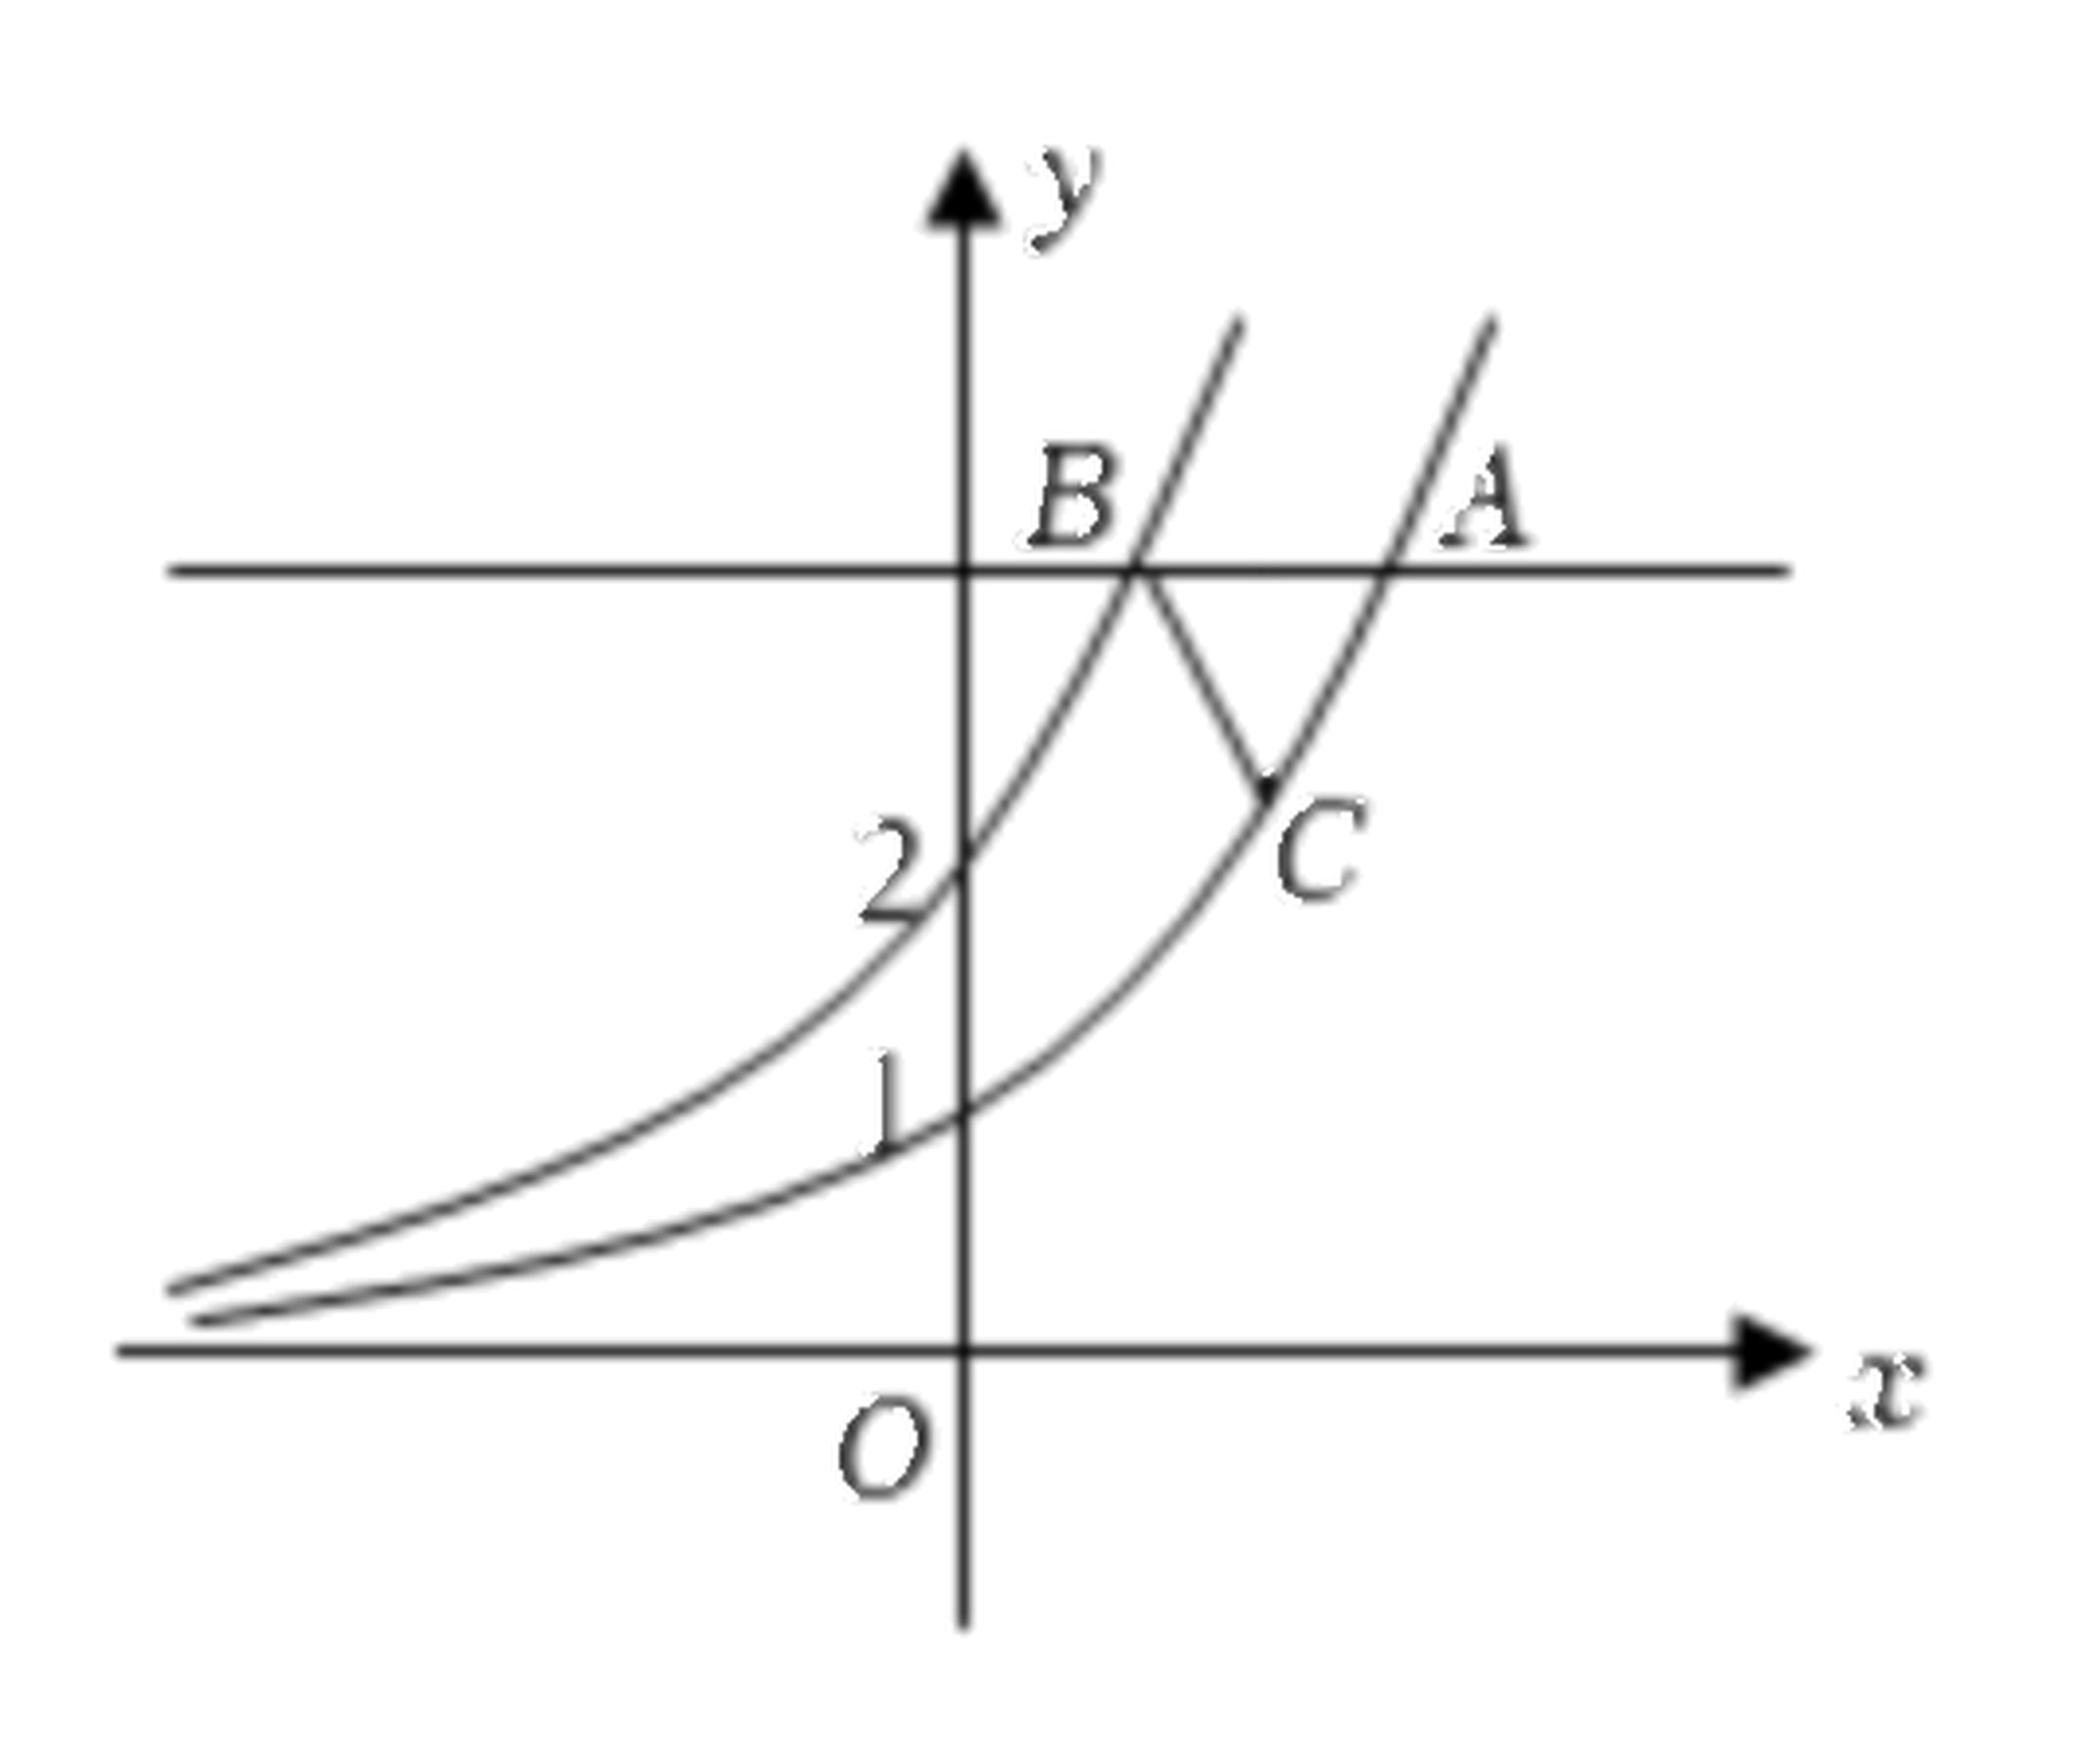
\includegraphics[width=0.40\textwidth]{figures/gao150_q11.png}
\end{center}

\ifanswer
\solbegin
\step{设直线 $l$ 的方程为 $y=a(a>0)$，}
\step{由 $2^x=a$，得 $x=\log_2 a$，所以 $A(\log_2 a,a)$，}
\step{由 $2^{x+1}=a$，得 $x=\log_2 a-1$，所以 $B(\log_2 a-1,a)$，所以 $\lvert AB\rvert=1$，}
\step{取 $AB$ 的中点 $D$，连接 $CD$，如图所示，}
\step{因为 $\triangle ABC$ 为等边三角形，则 $CD\perp AB$，且 $\lvert CD\rvert=\dfrac{\sqrt3}{2}$，}
\step{所以 $C\left(\log_2 a-\dfrac{1}{2},a-\dfrac{\sqrt3}{2}\right)$，}
\step{因为点 $C$ 在函数 $y=2^x$ 的图像上，所以 $a-\dfrac{\sqrt3}{2}=2^{\log_2 a-\frac{1}{2}}=\dfrac{a}{\sqrt2}$，}
\step{解得 $a=\dfrac{\sqrt3}{2-\sqrt2}=\dfrac{\sqrt3(2+\sqrt2)}{4-2}=\sqrt3+\dfrac{\sqrt6}{2}$，}
\step{所以点 $C$ 的纵坐标为 $a-\dfrac{\sqrt3}{2}=\dfrac{\sqrt3+\sqrt6}{2}$.}
\solend
\fi

% === Q12 === 解析配图（高斯函数方格阴影，仅答案版出）；"数学王子"弯引号；cases 块整体算一个印刷行；解析 4 行
\item 小玲在研究数学发展史，特别崇拜近代数学奠基者之一、享有“数学王子”称号的德国数学家高斯. 为了纪念高斯，我们把取整函数 $y=[x]$ 称为高斯函数，其中 $[x]$ 表示不超过 $x$ 的最大整数，如 $[1.1]=1$，$[-1.1]=-2$，则点集 $P=\{(x,y)\mid [x]^2+[y]^2=1\}$ 所表示的平面区域的面积为\blankline[4.4em].

\ifanswer
\solbegin
\step{$[x]^2+[y]^2=1$ 由 $\begin{cases}[x]=0\\ {[y]=-1}\end{cases}$ 或 $\begin{cases}[x]=0\\ {[y]=1}\end{cases}$ 或 $\begin{cases}[x]=-1\\ {[y]=0}\end{cases}$ 或 $\begin{cases}[x]=1\\ {[y]=0}\end{cases}$ 四个平面区域组成，}
\step{即 $\begin{cases}0\leqslant x<1\\ -1\leqslant y<0\end{cases}$ 或 $\begin{cases}0\leqslant x<1\\ 1\leqslant y<2\end{cases}$ 或 $\begin{cases}-1\leqslant x<0\\ 0\leqslant y<1\end{cases}$ 或 $\begin{cases}1\leqslant x<2\\ 0\leqslant y<1\end{cases}$，}
\step{作出平面区域如图所示，平面区域由四个边长为 $1$ 的正方形组成，}
\begin{center}
% 高斯函数 [x]^2+[y]^2=1 方格阴影区域图取 04 页顶部，去粉色水印、去色、4× LANCZOS 放大；仅答案版出
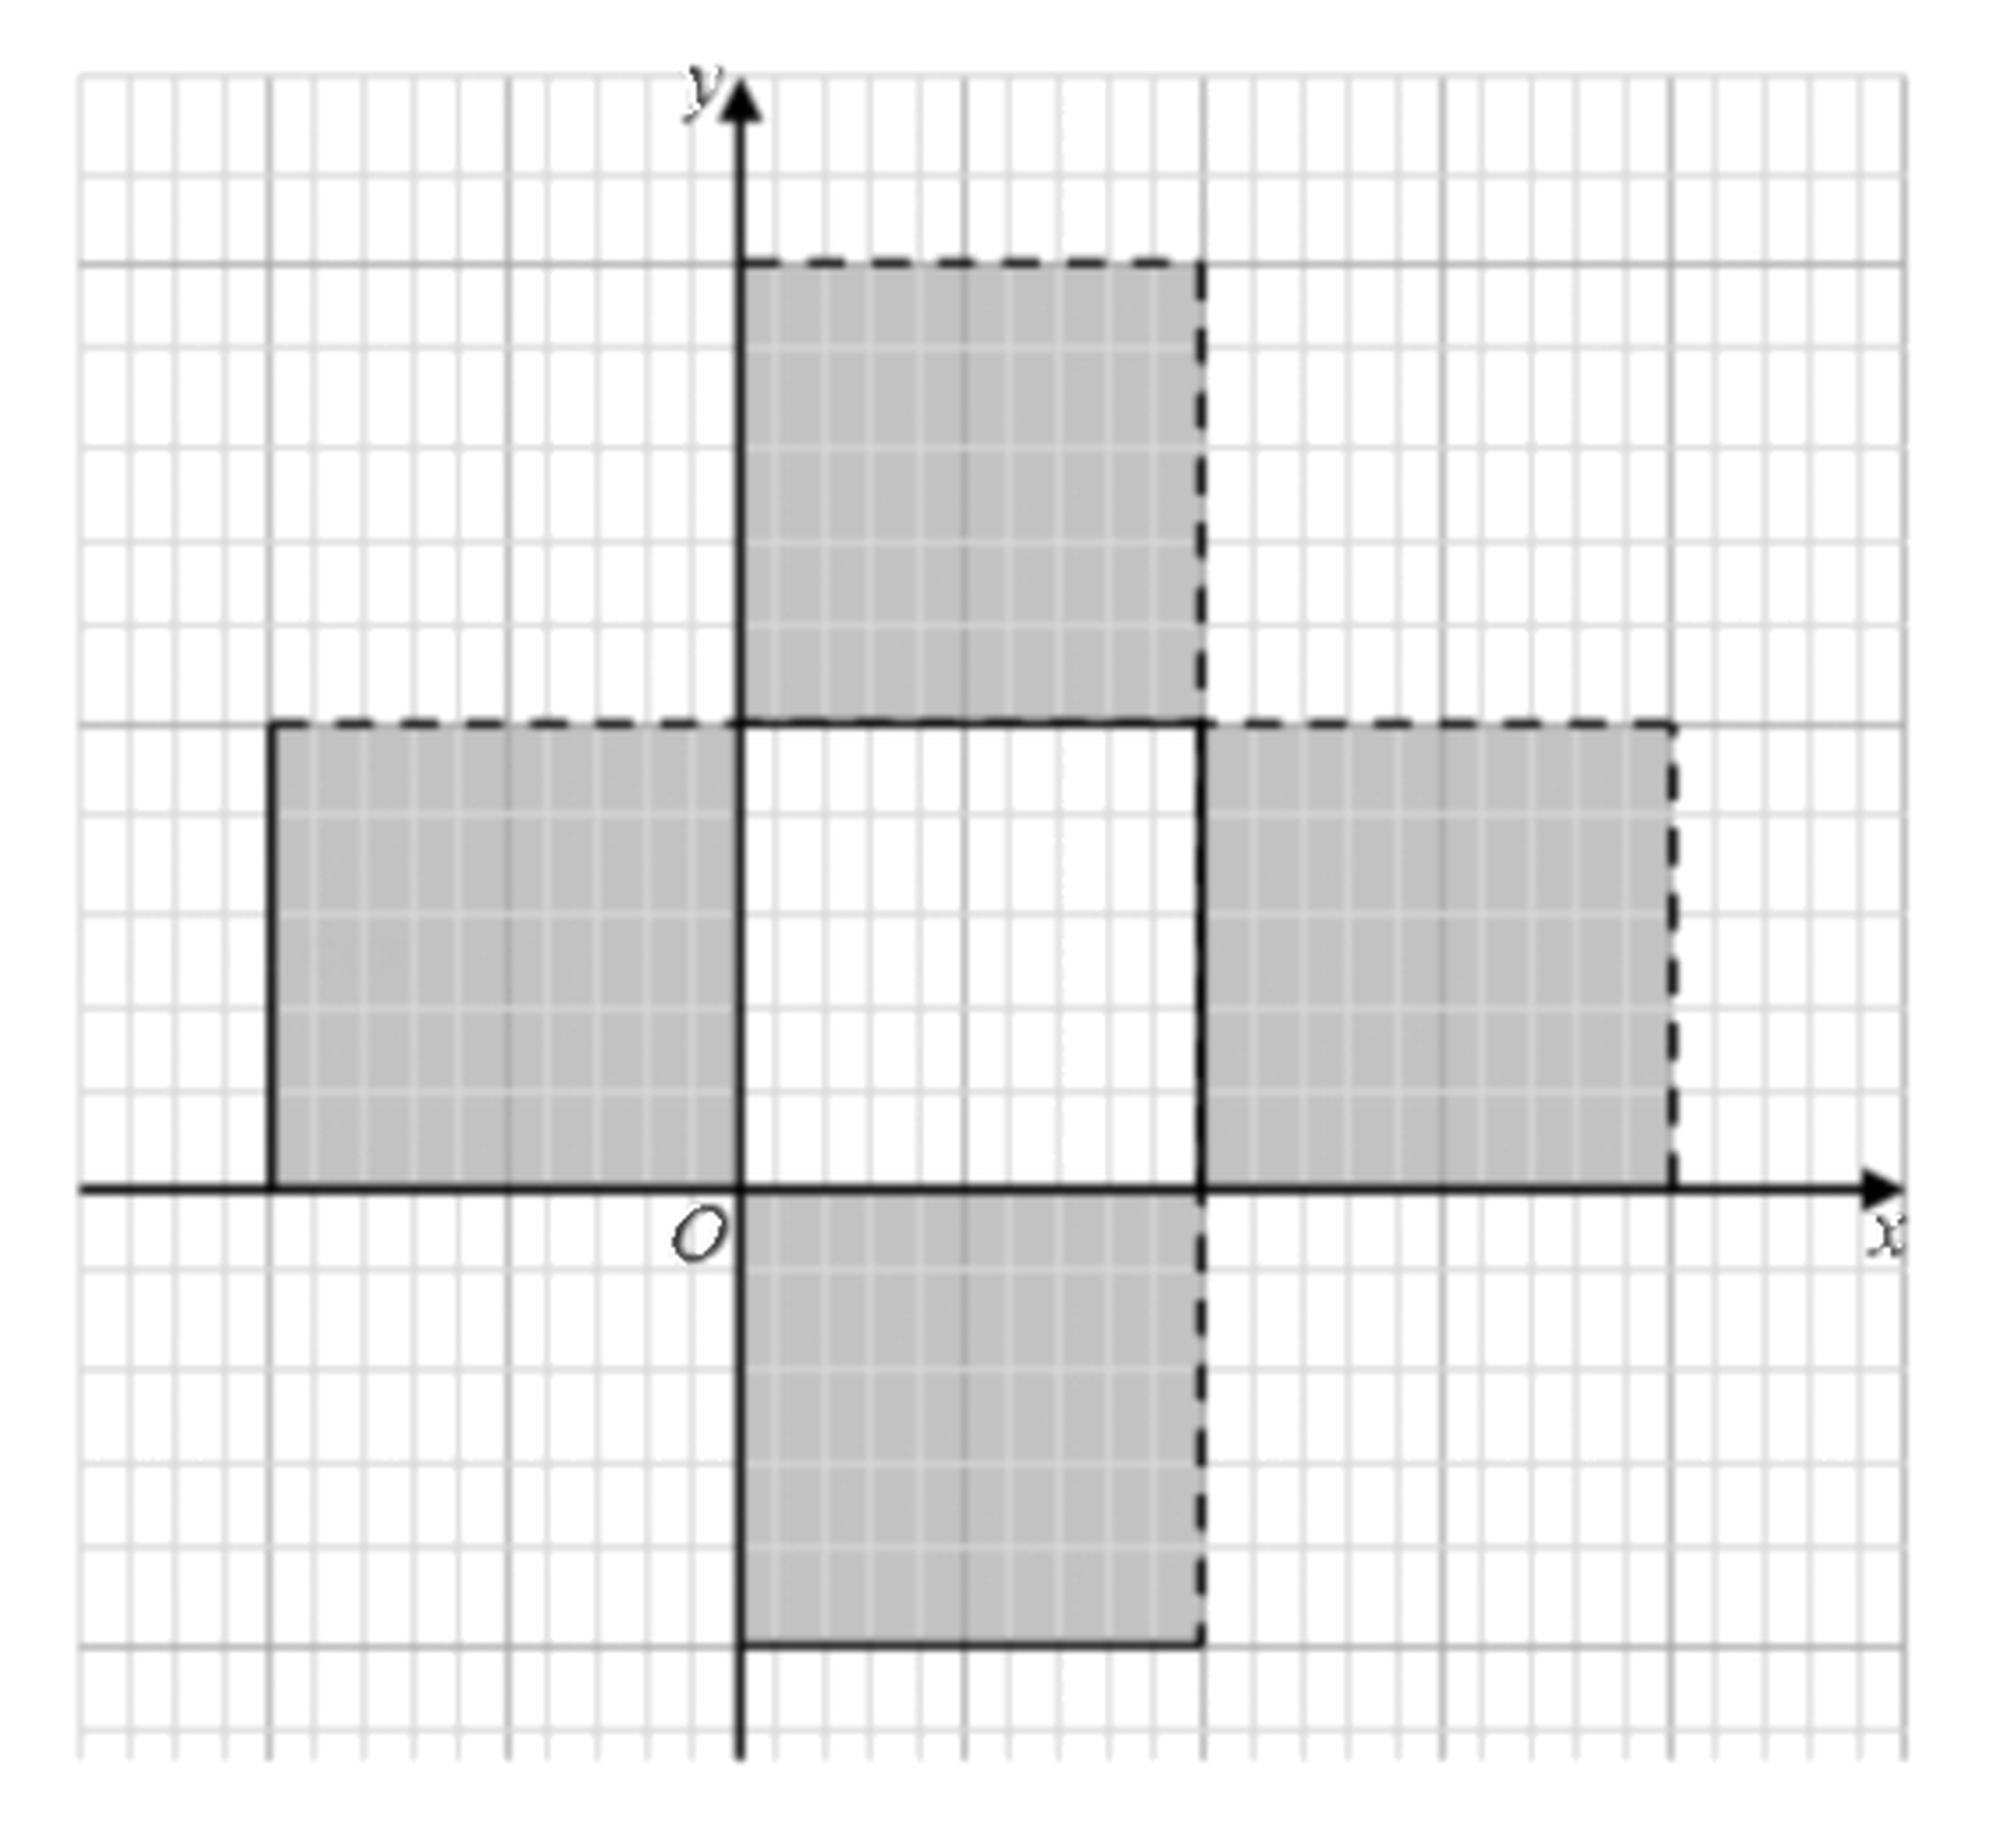
\includegraphics[width=0.34\textwidth]{figures/gao150_q12.png}
\end{center}
\step{总面积为 $1\times4=4$.}
\solend
\fi

\end{enumerate}

\bigsec{二、选择题}

\begin{enumerate}
\setcounter{enumi}{12}

% === Q13 === 答案在解析末句"故选 C"；括号 \mbox{（\quad）} 留空；四选项一行；解析 1 行
\item 设 $x\ne0$，则 $3^{\log_9 x^2}$ 的化简结果是\mbox{（\quad）}

\keepwithprev
A. $x$\qquad B. $\dfrac{1}{x}$\qquad C. $\lvert x\rvert$\qquad D. $\dfrac{1}{\lvert x\rvert}$

\ifanswer
\solbegin
\step{$3^{\log_9 x^2}=3^{\log_3\lvert x\rvert}=\lvert x\rvert$，故选 $C$.}
\solend
\fi

% === Q14 === 题目配图（两函数图像，三版都出）；\needvspace{8cm} 守卫放 \item 之前；"图像"照录；四选项两行两列；解析 2 行，故选 B
\needvspace{8cm}
\item 设 $a>0$ 且 $a\ne1$，$b\in\R$. 若函数 $y=a^{-\lvert x\rvert}$ 与 $y=x^b$ 的大致图像如图所示，则\mbox{（\quad）}

\keepwithprev
A. $0<a<1<b$\qquad\qquad B. $a>1$ 且 $b>1$

C. $0<a<1$ 且 $0<b<1$\qquad\qquad D. $0<b<1<a$

\begin{center}
% 两函数 y=a^{-|x|} 与 y=x^b 大致图像取 04 页右侧，去粉色水印、去色、4× LANCZOS 放大；三版都出
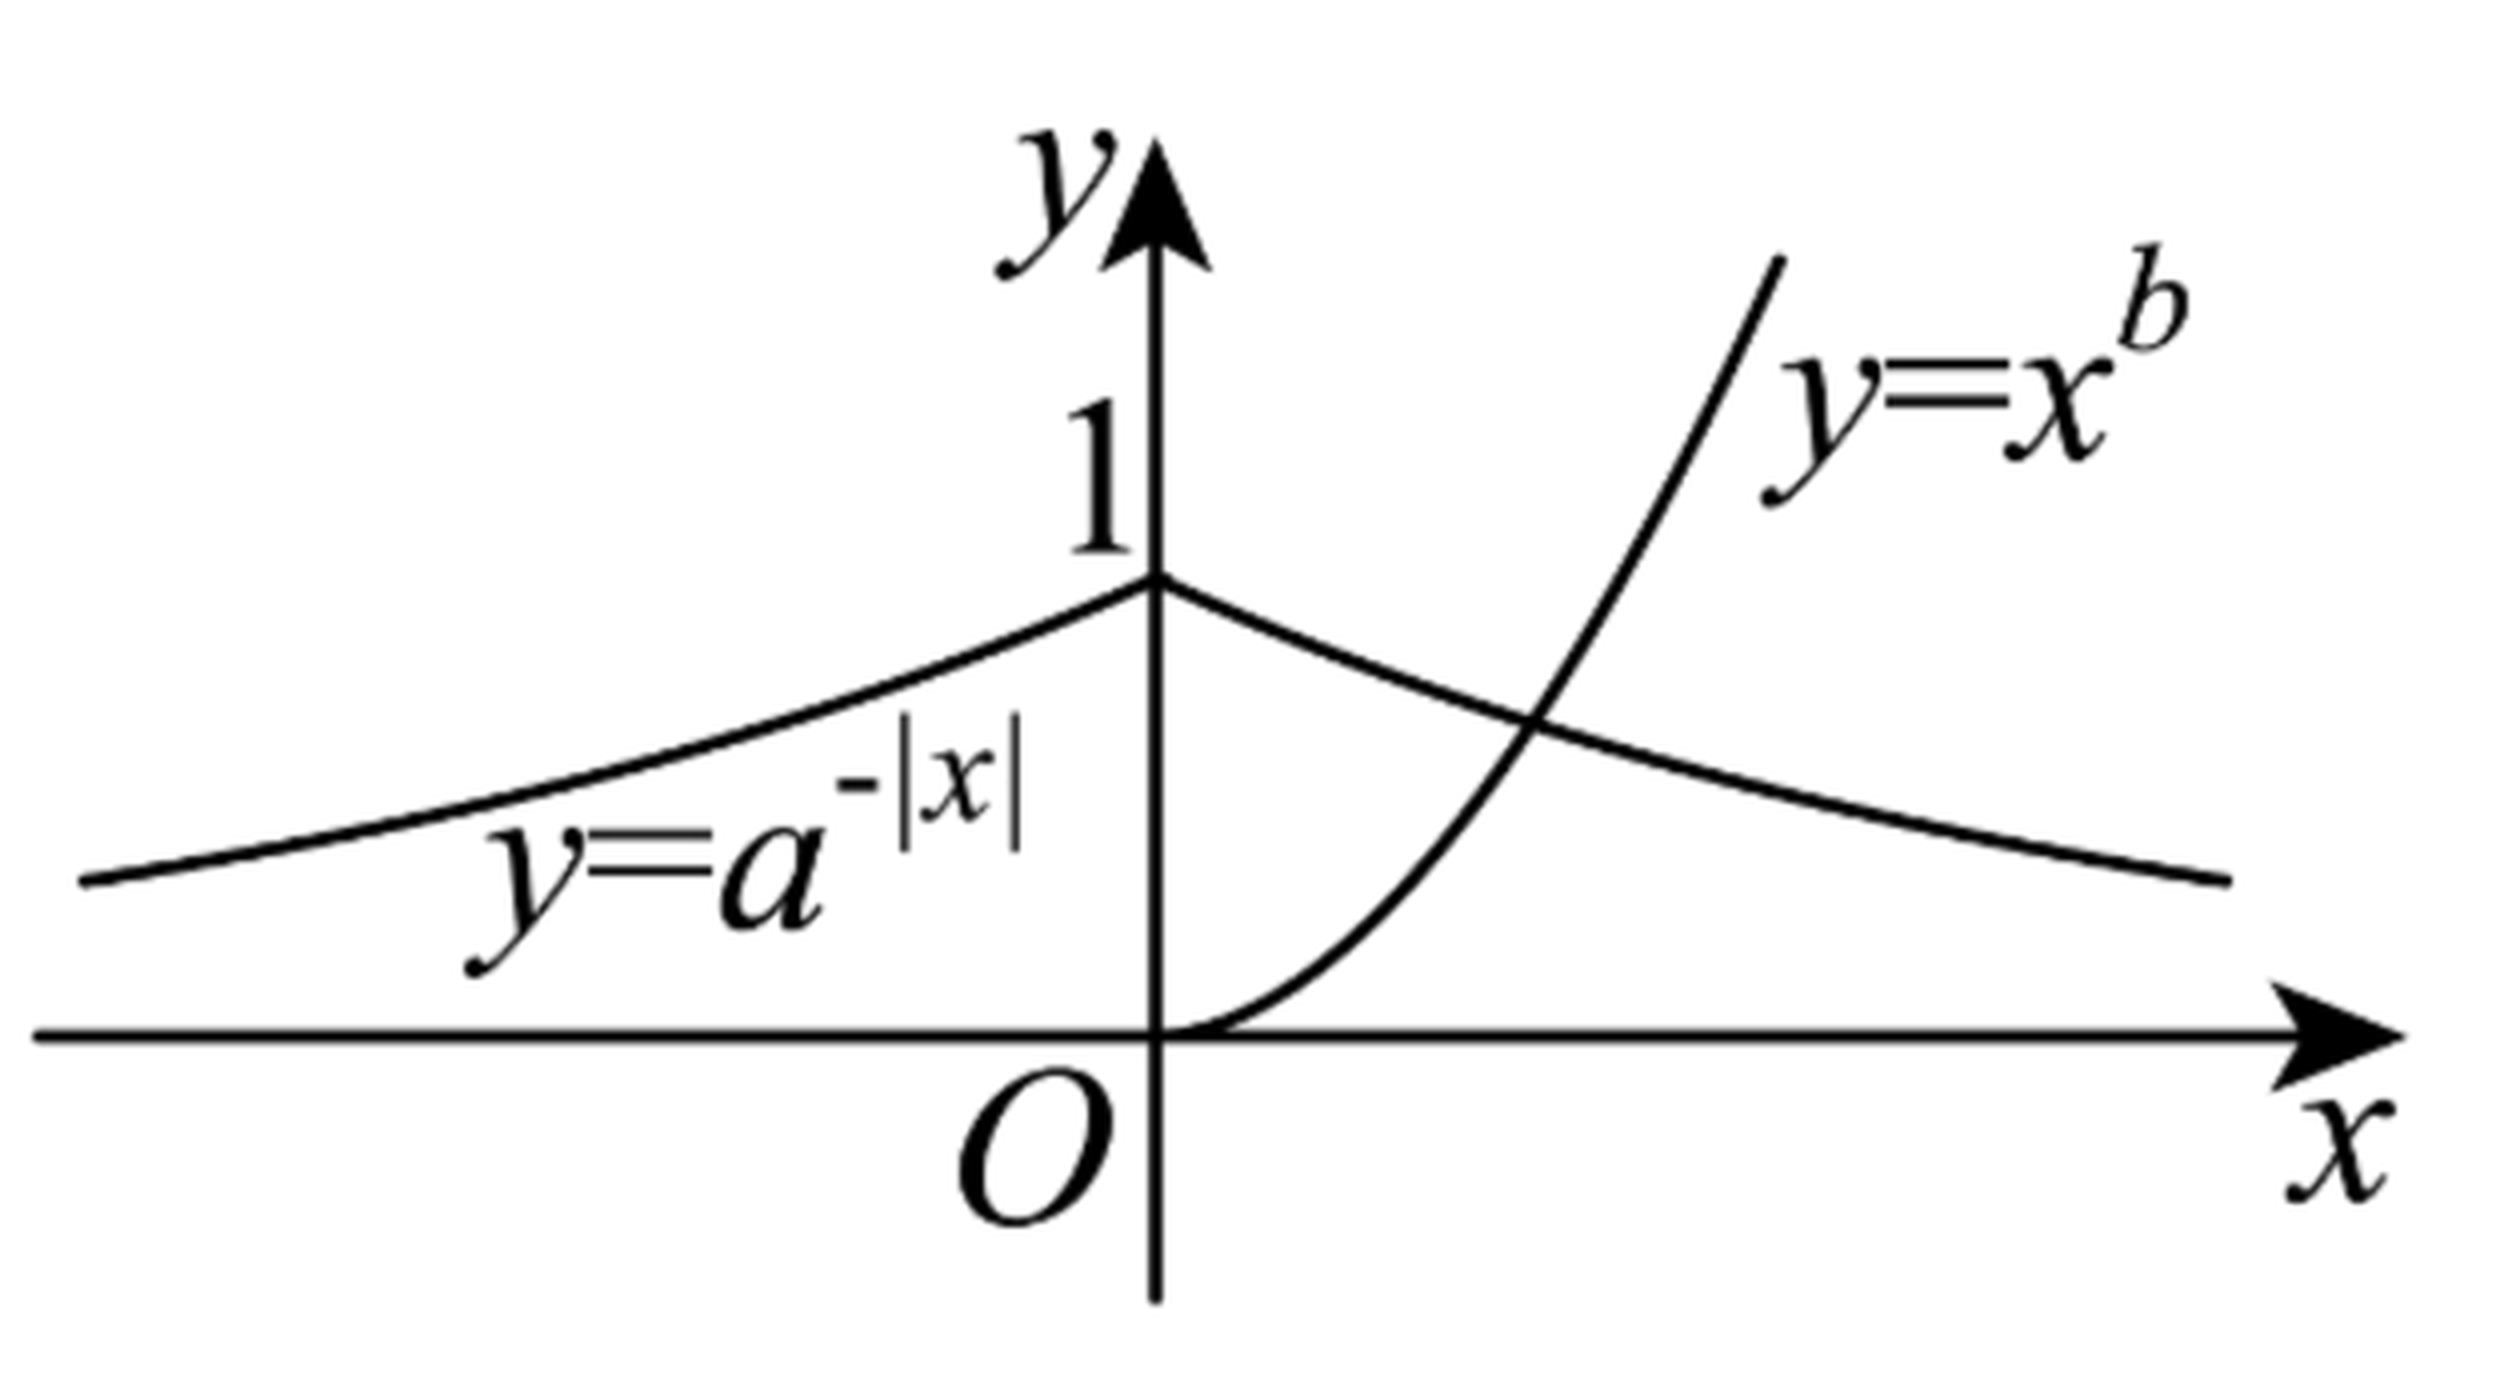
\includegraphics[width=0.40\textwidth]{figures/gao150_q14.png}
\end{center}

\ifanswer
\solbegin
\step{在 $(0,+\infty)$ 上，$y=a^{-x}$ 严格递减，得 $a>1$；}
\step{幂函数 $y=x^b$ 的图像递增且向上弯曲，得 $b>1$；故选 $B$.}
\solend
\fi

% === Q15 === "算术平均值／算术平均数"两处不同照录；四选项两行两列；解析 5 行（续 05 页顶），故选 B
\item 已知两个正数的算术平均值不小于它们的几何平均值，类比有以下结论：三个正数的算术平均数不小于它们的几何平均数，即当 $a,b,c$ 为正实数时，$\dfrac{a+b+c}{3}\geqslant\sqrt[3]{abc}$，当且仅当 $a=b=c$ 时等号成立. 利用上述结论，下列选项中判断正确的是\mbox{（\quad）}

\keepwithprev
A. 若 $x>0$，则 $2x+\dfrac{1}{x^2}\geqslant\dfrac{27}{8}$\qquad\qquad B. 若 $x>0$，则 $x^2+\dfrac{2}{x}\geqslant3$

C. 若 $0<x<1$，则 $x^2(1-x)\geqslant\dfrac{1}{9}$\qquad\qquad D. 若 $0<x<1$，则 $x^2(1-x)\leqslant\dfrac{1}{9}$

\ifanswer
\solbegin
\step{A：取 $x=1$，$2x+\dfrac{1}{x^2}=3<\dfrac{27}{8}$，错误.}
\step{B：$x^2+\dfrac{2}{x}=x^2+\dfrac{1}{x}+\dfrac{1}{x}\geqslant3\sqrt[3]{x^2\cdot\dfrac{1}{x}\cdot\dfrac{1}{x}}=3$，当且仅当 $x=1$ 时取等号，正确.}
\step{C：取 $x=\dfrac{1}{3}$，$x^2(1-x)=\dfrac{2}{27}<\dfrac{1}{9}$，错误.}
\step{D：取 $x=\dfrac{2}{3}$，$x^2(1-x)=\dfrac{4}{27}>\dfrac{1}{9}$，错误.}
\step{故选 $B$.}
\solend
\fi

% === Q16 === "完美集"新定义（弯引号、引号外空格照录）；圈数字①②文本模式；$n\in\N$；四选项两行两列；解析 9 行（6 行 05 页＋3 行 06 页顶），故选 A
\item 已知有限集 $A=\{a_1,a_2,\cdots,a_n\}$（$n\geqslant2$，$n\in\N$）. 若 $A$ 中元素 $a_i$（$i=1,2,\cdots,n$）满足 $a_1+a_2+\cdots+a_n=a_1\cdot a_2\cdots a_n$，就称 $A$ 为 “完美集”. 现有以下两个命题：

①恰有两个元素的 “完美集” 有无穷多个；

②若 $a_i$ 均为正整数，则 “完美集” $A$ 有且只有一个，且 $n=3$.

则\mbox{（\quad）}

\keepwithprev
A. ①和②都是真命题\qquad\qquad B. ①和②都是假命题

C. ①是真命题，②是假命题\qquad\qquad D. ①是假命题，②是真命题

\ifanswer
\solbegin
\step{①由 $a+b=ab\Leftrightarrow(a-1)(b-1)=1$，任取 $a>2$，则 $b=1+\dfrac{1}{a-1}\in(1,2)$，}
\step{得到无穷多个不同的完美集，①真.}
\step{②设 $1\leqslant a_1<a_2<\cdots<a_n$，则 $a_i\geqslant i$.}
\step{若 $n=2$，则 $(a_1-1)(a_2-1)=1$，只能有 $a_1=a_2=2$，与元素互异矛盾.}
\step{若 $n\geqslant4$，则 $a_1a_2\cdots a_n\geqslant a_2a_{n-1}a_n\geqslant2(n-1)a_n>na_n\geqslant a_1+\cdots+a_n$，矛盾.}
\step{当 $n=3$ 时，若 $a_1\geqslant2$，则 $a_1a_2a_3\geqslant6a_3>3a_3\geqslant a_1+a_2+a_3$，矛盾.}
\step{因此 $a_1=1$，$(a_2-1)(a_3-1)=2$，结合 $a_2<a_3$ 得 $a_2=2$，$a_3=3$.}
\step{唯一的完美集为 $\{1,2,3\}$，②真.}
\step{故选 $A$.}
\solend
\fi

\end{enumerate}

\bigsec{三、解答题}

\begin{enumerate}
\setcounter{enumi}{16}

% === Q17 === \varnothing 空集、$B\subseteq A$ 带下划线照录；弯引号内空格照录；解析 7 行
\item 设 $a,b\in\R$. 已知集合 $A=\{x\mid ax^2+3x-a>3\}$，$B=\{x\mid bx=1\}$.

(1) 若 $A=(1,2)$，求 $a$ 的值；

(2) 若 $a=0$，且 “ $x\in A$ ” 是 “ $x\in B$ ” 的必要非充分条件，求 $b$ 的取值范围.

\ifanswer
\solbegin
\step{(1) $A=(1,2)$，则 $a<0$，且 $1,2$ 是方程 $ax^2+3x-a-3=0$ 的两根.}
\step{由 $4a+6-a-3=0$，得 $a=-1$，此时不等式为 $-(x-1)(x-2)>0$，}
\step{解集确为 $(1,2)$.}
\step{(2) $a=0$ 时，$A=(1,+\infty)$，题意等价于 $B\subseteq A$ 且 $B\ne A$.}
\step{当 $b=0$ 时，$B=\varnothing$，符合条件.}
\step{当 $b\ne0$ 时，$B=\left\{\dfrac{1}{b}\right\}$，条件等价于 $\dfrac{1}{b}>1$，解得 $0<b<1$.}
\step{因此 $b$ 的取值范围为 $[0,1)$.}
\solend
\fi

% === Q18 === $p\in\Z$；"图像"（像，有亻）照录；指数 $-2p^2+5p$；解析 8 行（(1) 首行 06 页末＋2 行 07 页顶、(2) 5 行 07 页）
\item 设 $p\in\Z$，已知 $f(x)=x^{-2p^2+5p}$.

(1) 若幂函数 $y=f(x)$ 的图像关于原点成中心对称，且满足 $f(3)<f(4)$，求 $p$ 的值；

(2) 当 $p=-2$ 时，求满足 $f(2x+3)<f(x-4)$ 的 $x$ 的取值范围.

\ifanswer
\solbegin
\step{(1) 图像关于原点成中心对称，得整数 $-2p^2+5p$ 为奇数.}
\step{由 $f(3)<f(4)$，得 $-2p^2+5p>0\Leftrightarrow0<p<\dfrac{5}{2}$，}
\step{结合 $p\in\Z$，得 $p=1$ 或 $p=2$，对应指数分别为 $3$、$2$，所以 $p=1$.}
\step{(2) 当 $p=-2$ 时，$f(x)=\dfrac{1}{x^{18}}$，定义域为 $\{x\in\R\mid x\ne0\}$.}
\step{原不等式要求 $x\ne-\dfrac{3}{2}$ 且 $x\ne4$，}
\step{此时 $\dfrac{1}{(2x+3)^{18}}<\dfrac{1}{(x-4)^{18}}\Leftrightarrow\lvert 2x+3\rvert>\lvert x-4\rvert\Leftrightarrow(2x+3)^2>(x-4)^2$，}
\step{因此 $(x+7)(3x-1)>0\Leftrightarrow x<-7$ 或 $x>\dfrac{1}{3}$，}
\step{排除 $x=4$，得 $x\in(-\infty,-7)\cup\left(\dfrac{1}{3},4\right)\cup(4,+\infty)$.}
\solend
\fi

% === Q19 === $a\in\R$、$g(x)=f(2x+1)+a\cdot f(x)+2$；解析 6 行（(2) 末两行续 08 页顶）
\item 已知 $f(x)=2^x$.

(1) 求方程 $f(2x)-f(x)=6$ 的解；

(2) 设 $a\in\R$，$g(x)=f(2x+1)+a\cdot f(x)+2$，若对于任意 $x\in[-1,1]$，均有 $g(x)\geqslant1$，求 $a$ 的取值范围.

\ifanswer
\solbegin
\step{(1) 令 $t=2^x>0$，则 $t^2-t-6=(t-3)(t+2)=0$，}
\step{由 $t>0$ 得 $t=3$，所以 $x=\log_2 3$.}
\step{(2) 令 $t=2^x$，则 $t\in\left[\dfrac{1}{2},2\right]$，且 $g(x)\geqslant1\Leftrightarrow2t^2+at+1\geqslant0\Leftrightarrow a\geqslant-\left(2t+\dfrac{1}{t}\right)$，}
\step{由基本不等式得 $2t+\dfrac{1}{t}\geqslant2\sqrt{2t\cdot\dfrac{1}{t}}=2\sqrt2$，}
\step{当且仅当 $t=\dfrac{1}{\sqrt2}\in\left[\dfrac{1}{2},2\right]$ 时等号成立，}
\step{因此 $-\left(2t+\dfrac{1}{t}\right)$ 的最大值为 $-2\sqrt2$，所求范围为 $a\in[-2\sqrt2,+\infty)$.}
\solend
\fi

% === Q20 === "极闭集"新定义、3 问，全卷末题；$M\subseteq(0,+\infty)$ 带下划线照录；自定义运算 $x*y$ 星号照录；解析 13 行（9 行 08 页＋4 行 09 页上半）
\item 对于非空实数集 $M\subseteq(0,+\infty)$，若满足以下两个条件：

① $M$ 中至少含有 $2$ 个元素，且 $1\notin M$；

②对于 $M$ 中任意两个不相等的元素 $x$、$y$，定义 $x*y=\dfrac{xy+1}{x+y}$，且 $x*y\in M$.

则称 $M$ 为 “极闭集”.

(1) 分别判断集合 $A=\left\{\dfrac{1}{2},3\right\}$ 与集合 $B=(1,+\infty)$ 是否为 “极闭集” （无需理由）；

(2) 若 $M$ 是 “极闭集”，证明：$M$ 中不可能所有元素都小于 $1$；

(3) 证明：不存在任何有限集是 “极闭集”.

\ifanswer
\solbegin
\step{(1) $A$ 不是 “极闭集”，$B$ 是 “极闭集”.}
\step{(2) 假设 $M$ 中所有元素都小于 $1$，取其中两个不相等的元素 $x$、$y$，}
\step{则 $x*y-1=\dfrac{(1-x)(1-y)}{x+y}>0$，}
\step{这与 $x*y\in M$ 且 $M$ 中所有元素都小于 $1$ 矛盾.}
\step{(3) 假设有限集 $M$ 是 “极闭集”，}
\step{由 (2) 及 $1\notin M$，得 $M$ 中存在大于 $1$ 的元素.}
\step{若 $M$ 中有小于 $1$ 的元素，取其中最大的一个为 $a$，另取 $b\in M$ 且 $b>1$，}
\step{则 $a*b-a=\dfrac{1-a^2}{a+b}>0, a*b-1=\dfrac{(a-1)(b-1)}{a+b}<0$，}% 半角逗号在两个数学式组之间，全稿惯例、非笔误，照录
\step{于是 $a<a*b<1$ 且 $a*b\in M$，与 $a$ 的最大性矛盾.}
\step{若 $M$ 中没有小于 $1$ 的元素，则 $M\subseteq(1,+\infty)$.}
\step{取 $a=\min M$，另取 $b\in M$ 且 $b\ne a$，则 $a*b-a=\dfrac{1-a^2}{a+b}<0$，}
\step{于是 $a*b<a$ 且 $a*b\in M$，与 $a$ 的最小性矛盾.}
\step{因此不存在任何有限集是 “极闭集”.}
\solend
\fi

\end{enumerate}

\end{document}
"
% 紧凑版：xelatex "\def\iscompact{1}% 高一150_曹杨二中_期中.tex
%   —— 高一上数学"2026-2027 年曹杨二中高一上期中"（试卷版/答案版/紧凑版）
% 试卷版：xelatex 高一150_曹杨二中_期中.tex
% 答案版：xelatex "\def\isanswer{1}% 高一150_曹杨二中_期中.tex
%   —— 高一上数学"2026-2027 年曹杨二中高一上期中"（试卷版/答案版/紧凑版）
% 试卷版：xelatex 高一150_曹杨二中_期中.tex
% 答案版：xelatex "\def\isanswer{1}\input{高一150_曹杨二中_期中.tex}"
% 紧凑版：xelatex "\def\iscompact{1}\input{高一150_曹杨二中_期中.tex}"
%
% ① 原始材料：微信公众号"魔都数学加油站"文章，连载"27学年高一150"，原文标题
% "27学年高一150——2026-2027年上海市曹杨二中高一上期中"；
% 原文链接：https://mp.weixin.qq.com/s/xlQxmik8TZXR87RC6MnCrw 。
% 正文为 9 张 PNG 页（01/02/04/06/07/09 为 2560×3620，03/05/08 为 4762×6735，
% 同一篇各页分辨率混排，逐页按各自分辨率裁图核对，别按预览比例换算裁框）。
% 体例：讲评版——全 18 题均印【解析】（逐题核实，见 ② ②）。
% 题目、答案、解析均据原图转录；卷面粉红色/红色水印"魔都数学加油站"及公众号页脚未录入。
% 全卷插图清单（逐页通读 9 页确认）：3 幅——
%   · Q11 题目配图（指数函数曲线图，02 页右侧：x/y 轴、O、y=2^x 与 y=2^{x+1}
%     两曲线、A/B/C 三点、刻度 1/2、等边三角形 ABC），三版都出，裁 figures/gao150_q11.png；
%   · Q12 解析配图（高斯函数取整 [x]^2+[y]^2=1 方格阴影区域图，04 页顶部：4 个边长 1
%     的正方形组成的十字形阴影），解析"作出平面区域如图所示"处，仅答案版出，
%     放 \ifanswer 内 \step 之间，裁 figures/gao150_q12.png；
%   · Q14 题目配图（两函数 y=a^{-|x|} 与 y=x^b 大致图像，04 页右侧：x/y 轴、O、
%     y 轴刻度 1、一递减曲线一递增上翘曲线），三版都出，裁 figures/gao150_q14.png；
%   其余各页逐页确认无其它题目配图、无表格；Q11/Q12 解析"如图所示"对应的就是上列
%   已裁的图，不重复裁；09 页上半为 Q20(3) 解析续尾、下半仅水印、无正文。
%   3 图均取自原卷截图，去粉色水印、去色、4× LANCZOS 放大。
%
% 卷首标题：原卷印作"2026-2027 年曹杨二中高一上期中"，年份区间按全稿惯例排 en dash；
% 原卷卷面未印副标题，本稿按同期中卷知识模块口径补出"集合与常用逻辑用语、不等式、函数"。
%
% 题号体例（逐页核实定稿）：本卷共 18 题——一、填空题 3—12（10 题）、
% 二、选择题 13—16（4 题）、三、解答题 17—20（4 题）。
% 三节分别 \setcounter{enumi}{2}／{12}／{16}。原卷从第 3 题起、无第 1、2 题，
% 本稿保留原题号；全卷末题为第 20 题（"极闭集"新定义、3 问），无 Q21、无附加题节。
%
% ② 与原卷的排版差异：
%   ① 原文从第 3 题起，本稿保留原题号；共 18 题三节，解答题只有 4 题到 20；
%   ② 全 18 题均印【解析】，用 \solbegin…\solend；逐题核实无只印【答案】或
%      答案印题干括号内的题；四道选择题答案在解析末句"故选 X"（Q13 选 C、
%      Q14 选 B、Q15 选 B、Q16 选 A，逐个放大复核）、括号 \mbox{（\quad）} 留空、
%      不另提 \ans{}；答案版【答案】/【解析】标记数 = 18 = 全卷题数；
%   ③ 原卷卷面未印副标题，本稿按知识模块口径补出；
%   ④ 原卷填空横线按全稿惯例排 \blankline[4.4em]；选择题括号排 \mbox{（\quad）}、
%      选项段前按惯例加 \keepwithprev；解答题不留作答区、不加 \anspace（原卷为讲评版）；
%   ⑤ 数集黑板粗体：Q4"m\in R"、Q5"a,b\in R"、Q6"a,b,c\in R"、Q7"a\in R"、
%      Q10"a\in R"、Q14"b\in R"、Q17"a,b\in R"、Q18"p\in Z"／定义域"x\in R"、
%      Q19"a\in R"、Q16"n\in N" 原卷印斜体 R/Z/N，按全稿惯例归一 \R／\Z／\N；
%      绝对值排 \lvert…\rvert（Q7 |x+4|+|x-3|、Q11 |AB|／|CD|、Q13 |x|、
%      Q18 |2x+3|／|x-4|），集合描述竖线排 \mid（Q3、Q12、Q17、Q18、Q20），
%      不等号按全稿惯例排 \leqslant／\geqslant；补集照原卷上划线排 \overline{A}
%      （Q3 题干＋解析共 2 处）；空集符号 \varnothing（Q17 解析(2)）；
%      子集 \subset（单线⊂）／\subseteq（带下划线⊆）逐处照录，本卷 3 处子集
%      符号均印带下划线 ⊆、照录 \subseteq（Q20 题干、Q20 解析(3)、Q17 解析(2)，
%      见 ④），无 \subset 用例；
%   ⑥ 判别式 Δ/△：逐页通读 9 页，本卷无一元二次判别式算式，故无 Δ/△ 混用可照录
%      （"高 \Delta／扁 \triangle"口径备查，参照 高一142／144／145／146／148／149
%      头注④）；本卷仅 Q11 题干与解析共 2 处几何三角形符号 △ABC，逐处放大并排
%      确认两处同形、印近等边粗线三角（非判别式），照录 \triangle（见 ④）；
%   ⑦ 中文弯引号照录：Q12"数学王子"、Q16"完美集"（题干＋①②两命题，引号外
%      留空格）、Q17" x∈A "" x∈B "（引号内空格）、Q20"极闭集"（题干条件、
%      三问与解析，引号外留空格）；注释里一律 ASCII 引号；数学式内 CJK 用 \text{}
%      （Q3 集合描述"且"用 \text{ 且 }）；
%   ⑧ 半角逗号在数学组之间是全稿惯例、非笔误，逐处照录（Q17 解析"1,2 是方程…
%      两根"、Q20 解析(3)">0, a*b-1=…<0" 两式之间等）；行末西文句点 ASCII `.`；
%      行中全角逗号／顿号照录（Q12"之一、享有"、Q18 解析"3、2"、Q20"x、y"）；
%   ⑨ "图像／图象"逐处放大核：全卷 9 处均印"图像"（像，有亻）、未见"图象"——
%      Q4 题干 1、Q11 题干 2＋解析 1、Q14 题干 1＋解析 1、Q18 题干 1＋解析 1；
%      同卷"第二象限""象限"用"象"（无亻）。逐处照录未统一改动（放大 01/02/04/06
%      页 /tmp/gao150/z/p01_q4_tuxiang2.png、p04_q14_tuxiang2.png、
%      p02_q11_lines.png 确认）；子题标号 (1)(2)(3) 半角括号照录；圈数字①②
%      在文本模式（Q16 两命题与解析、Q20 两条件与三问及解析）按 common.sty
%      划入 CJK 字符类渲染，进数学式用 \text{①}；
%   ⑩ Q20 新定义 x*y=\dfrac{xy+1}{x+y} 的 * 是自定义运算（星号），照录；
%      \left…\right 不得拆到不同 $…$ 组（Q19"\left(2t+\frac1t\right)"、
%      Q20 题干"A=\left\{\frac12,3\right\}"等）；Q8 嵌套根号
%      \sqrt{\frac2x+\frac{16}{1-2x}}、Q9 对数连加 \log_2 A 等复杂式照录别简化；
%   ⑪ 一条 \step = 原卷解析的一个印刷行，cases 块整体算一个印刷行；别并折行、
%      别拆行。Q4 三行、Q8 五行、Q11 九行、Q12 四行（两行各含四个 cases 块）、
%      Q15 五行、Q16 九行、Q18 八行、Q20 十三行均按印刷行逐条断，不丢行；
%   ⑫ 配图：Q11／Q14 题目配图（三版都出）放 \item 内题干之后 \begin{center}，
%      大图块加 \needvspace{8cm} 守卫把整块推走（守卫放 \item 之前，见
%      高一145 Q14/Q20 成例与切页审计 B 类坑）；Q12 解析配图（仅答案版出）
%      放 \ifanswer 内 \solbegin…\solend 的 \step 之间（高一73 第16题成例）；
%   ⑬ 跨页续印按题合并：见 ⑥；
%   ⑭ 原卷解析内无红色"法一／法二"之类小标题，故本卷无 \stepm；红色水印
%      "魔都数学加油站"不录入；Q12 解析"作出平面区域如图所示"对应的图即
%      ① 所列 gao150_q12.png（04 页顶部），不重复裁；Q11 解析"如图所示"对应
%      题目配图 gao150_q11.png，不另裁。
%
% ③ 行数复核：一条 \step／\stepm = 原卷解析的一个印刷行，cases 块作一个印刷行计。
%   逐题数（主会话逐页核对定稿）：Q3：1；Q4：3；Q5：2；Q6：1；Q7：2；Q8：5；
%   Q9：1；Q10：3；Q11：9；Q12：4；Q13：1；Q14：2；Q15：5；Q16：9；
%   Q17：7；Q18：8；Q19：6；Q20：13。
%   合计 82 条 \step（本卷无 \stepm：解析内无红色"法一／法二"类小标题），
%   与原卷逐题印刷行相等。全卷 18 题均设 \solbegin…\solend，答案版
%   【答案】/【解析】标记数 = 18 = 全卷题数。
%
% ④ 判别式／三角形／子集符号结论（逐处放大原图照录、不得统一，主会话像素级复核）：
%   判别式：逐页通读 9 页，本卷无一元二次判别式 Δ/△ 算式（Q18 讨论幂函数指数
%     奇偶、不用判别式；Q9／Q19／Q20 亦无），头注 ② ⑥ 的"高 \Delta／扁 \triangle"
%     口径在本卷无对应处（参照 高一142／144／145／146／148／149 头注④，仅备查）。
%   几何三角形符号：Q11 题干"使得 △ABC 为等边三角形"（02 页末）与解析
%     "因为 △ABC 为等边三角形，则 CD⊥AB"（03 页）共 2 处，放大 02/03 页
%     /tmp/gao150/z/q11_tri_montage2.png 并排确认两处同形、印近等边粗线三角
%     （h/w≈0.98、非"高>宽"的判别式 \Delta），照录 \triangle（与 高一105
%     "使得 \triangle ABC 为等边三角形" 同短语成例、高一149 几何三角形照录
%     \triangle 口径一致），不引入 \Delta。
%   子集／补集：Q20 题干"$M\subseteq(0,+\infty)$"（08 页）、Q20 解析(3)
%     "则 $M\subseteq(1,+\infty)$"（09 页）、Q17 解析(2)"题意等价于 $B\subseteq A$
%     且 $B\ne A$"（06 页）共 3 处子集符号，逐处放大（/tmp/gao150/z/p08_q20_stem.png、
%     p09_q20_sub.png、p06_q17_sub.png）确认均印带下划线 ⊆，照录 \subseteq；
%     本卷未见单线 ⊂（\subset）之对应处。Q3 题干与解析共 2 处补集照原卷上划线
%     排 \overline{A}；Q17 解析(2) 空集印 ∅、照录 \varnothing（Q7"解集为空集"
%     为中文词、非符号，照录文字）；集合描述竖线 \mid；数集 \R／\Z／\N 归一见 ② ⑤。
%
% ⑤ 存疑照录（放大原图确认，照录未改、正文对应处另有 % 注）：
%   1. Q8 解析第 4 行"所以 $y=\frac1x+\frac{8}{1-2x}$ 的最小值为 18" —— 上文
%      并未定义 $y$，且题面求的是 $\sqrt{\frac2x+\frac{16}{1-2x}}$ 的最小值；
%      按上下文该行应为 $\frac1x+\frac{8}{1-2x}$ 的最小值为 18（$y$ 疑为原卷
%      衍字／笔误），放大 02 页 /tmp/gao150/z/p02_q8_y.png 确认，照录未改。
%   2. Q20 解析(3)"$a*b-a=\frac{1-a^2}{a+b}>0, a*b-1=\frac{(a-1)(b-1)}{a+b}<0$"
%      两式之间的逗号原卷印半角 ,（非全角），按全稿惯例"半角逗号在数学组之间"
%      照录未改（放大 08 页 /tmp/gao150/z/p08_q20_sol8.png 确认）。
%   3. Q15 题干"两个正数的算术平均值…几何平均值"与"三个正数的算术平均数…
%      几何平均数"两处"值／数"用字不同，逐处照录未统一（放大 04 页确认）。
%   4. "图像／图象"全卷 9 处均印"图像"（像，有亻）、未见"图象"，逐处放大核实
%      照录、未统一改动（见 ② ⑨）；本卷判别式 Δ/△ 无用例、几何三角形 2 处
%      照录 \triangle（见 ④）。
%   全卷除此 4 类外未发现其它笔误／自相矛盾处；18 题均印【解析】、无只印【答案】
%   或答案印题干括号内的题（见 ② ②）。
%
% ⑥ 跨页续印按题合并说明（逐页核实定稿）：Q3/4/5/6/7 题干＋解析在 01 页；
%   Q8 题干＋解析 5 行、Q9 题干＋解析 1 行在 02 页上半；Q10 题干＋解析 3 行
%   在 02 页下半；Q11 题干（前两行）＋配图在 02 页下半、题干续"三角形，则点 C
%   的纵坐标为___"与解析 9 行全在 03 页上半（解析"如图所示"对应题目配图）；
%   Q12 题干＋解析 4 行在 03 页下半，解析配图（方格阴影）续印在 04 页顶部；
%   "二、选择题"标题在 04 页中部；Q13 题干＋选项＋解析、Q14 题干＋选项＋
%   配图＋解析在 04 页；Q15 题干＋四选项在 04 页末、解析 5 行续 05 页上半；
%   Q16 题干＋①②两命题＋"则(  )"＋四选项＋解析前 6 行在 05 页、解析末 3 行
%   （"因此 a_1=1…②真""故选 A"）续 06 页顶部；"三、解答题"标题在 06 页；
%   Q17 题干(1)(2)＋解析(1) 3 行＋解析(2) 首行在 06 页、解析(2) 续 3 行
%   在 06 页下半；Q18 题干(1)(2)＋解析(1) 首行在 06 页末、解析(1) 续 2 行＋
%   解析(2) 5 行在 07 页上半；Q19 题干(1)(2)＋解析(1) 2 行＋解析(2) 前 2 行
%   在 07 页下半、解析(2) 末 2 行续 08 页顶部；Q20 题干（新定义＋①②两条件）
%   ＋三问＋解析(1)(2)(3) 前 9 行在 08 页、解析(3) 末 4 行续 09 页上半，
%   末行"因此不存在任何有限集是极闭集"为全卷收尾（09 页下半仅水印、无正文）。
%   本稿按题连排，不丢行、不并折行；全卷末题为第 20 题，无 Q21、无附加题节。
%
\documentclass[a4paper,11pt]{article}
\usepackage{common}

\begin{document}

\examtitlest[3]{2026--2027 年曹杨二中高一上期中}{集合与常用逻辑用语、不等式、函数}

\bigsec{一、填空题}

\begin{enumerate}
\setcounter{enumi}{2}

% === Q3 === 补集上划线 \overline{A}（题干＋解析各 1 处）；集合描述竖线 \mid、数学式内"且"用 \text{}；解析 1 行
\item 设全集 $U=\{1,2,3,4,5\}$，集合 $A=\{x\mid x^2-3x\leqslant0\text{ 且 }x\in U\}$，则 $\overline{A}=$\blankline[4.4em].

\ifanswer
\solbegin
\step{$x^2-3x\leqslant0\Leftrightarrow0\leqslant x\leqslant3$，所以 $A=\{1,2,3\}$，$\overline{A}=\{4,5\}$.}
\solend
\fi

% === Q4 === "图像"（像，有亻）逐处照录、同句"第二象限"用"象"（无亻）；解析 3 行
\item 设 $m\in\R$. 若幂函数 $y=(m^2-5m+1)x^{m+1}$ 的图像经过第二象限，则 $m=$\blankline[4.4em].

\ifanswer
\solbegin
\step{幂函数的系数为 1，故 $m^2-5m+1=1\Rightarrow m=0$ 或 $m=5$.}
\step{$m=0$ 时，$y=x$ 不经过第二象限；}
\step{$m=5$ 时，$y=x^6$ 经过第二象限，因此 $m=5$.}
\solend
\fi

% === Q5 === 解析 2 行
\item 设 $a,b\in\R$. 若 $a^2+\dfrac{b^2}{4}=1$，则 $ab$ 的最大值为\blankline[4.4em].

\ifanswer
\solbegin
\step{$1-ab=\left(a-\dfrac{b}{2}\right)^2\geqslant0$，即 $ab\leqslant1$；}
\step{当 $a=\dfrac{\sqrt2}{2}$，$b=\sqrt2$ 时取等号，最大值为 1.}
\solend
\fi

% === Q6 === 解析 1 行
\item 设 $a,b,c\in\R$. 若等式 $2x^2-3x-2=a(x-1)^2+b(x-1)+c$ 恒成立，则 $a-b+c=$\blankline[4.4em].

\ifanswer
\solbegin
\step{令 $x=0$，得 $a-b+c=-2$.}
\solend
\fi

% === Q7 === 绝对值 \lvert…\rvert；解析 2 行
\item 设 $a\in\R$. 若关于 $x$ 的不等式 $\lvert x+4\rvert+\lvert x-3\rvert<a$ 的解集为空集，则 $a$ 的取值范围是\blankline[4.4em].

\ifanswer
\solbegin
\step{$\lvert x+4\rvert+\lvert x-3\rvert\geqslant\lvert(x+4)-(x-3)\rvert=7$，当 $-4\leqslant x\leqslant3$ 时取等号.}
\step{原不等式的解集为空集当且仅当 $a\leqslant7$，即 $a\in(-\infty,7]$.}
\solend
\fi

% === Q8 === 嵌套根号 \sqrt{\frac{2}{x}+\frac{16}{1-2x}} 照录别简化；解析 5 行
\item 设 $x\in\left(0,\dfrac{1}{2}\right)$，则 $\sqrt{\dfrac{2}{x}+\dfrac{16}{1-2x}}$ 的最小值为\blankline[4.4em].

\ifanswer
\solbegin
\step{因为 $x\in\left(0,\dfrac{1}{2}\right)$，所以 $1-2x>0$，又 $2x+1-2x=1$，}
\step{所以 $\left(\dfrac{1}{x}+\dfrac{8}{1-2x}\right)(2x+1-2x)=10+\dfrac{1-2x}{x}+\dfrac{16x}{1-2x}$}
\step{$\geqslant10+2\sqrt{\dfrac{1-2x}{x}\cdot\dfrac{16x}{1-2x}}=18$，}
\step{当且仅当 $\dfrac{1-2x}{x}=\dfrac{16x}{1-2x}$ 即 $x=\dfrac{1}{6}$ 时取等号，所以 $y=\dfrac{1}{x}+\dfrac{8}{1-2x}$ 的最小值为 18，}% 原卷此处径写 $y=\frac1x+\frac{8}{1-2x}$（上文未定义 $y$、且与题面根式不符），疑笔误，放大 02 页确认，照录未改（见 ⑤）
\step{所以 $\sqrt{\dfrac{2}{x}+\dfrac{16}{1-2x}}$ 的最小值为 6.}
\solend
\fi

% === Q9 === 对数连加 \log_2 A 等复杂式照录别简化；解析 1 行
\item 记 $A=1\times2\times3\times\cdots\times2026$，则 $\dfrac{1}{\log_2 A}+\dfrac{1}{\log_3 A}+\dfrac{1}{\log_4 A}+\cdots+\dfrac{1}{\log_{2026}A}=$\blankline[4.4em].

\ifanswer
\solbegin
\step{原式 $=\log_A 2+\cdots+\log_A 2026=\log_A(2\times3\times\cdots\times2026)=\log_A A=1$.}
\solend
\fi

% === Q10 === "严格减函数／不恒为负／⇔"照录；解析 3 行
\item 设 $a\in\R$，$f(x)=\dfrac{ax+1}{x+2}$. 若函数 $y=f(x)$ 在 $[1,+\infty)$ 上是严格减函数，且在 $[1,+\infty)$ 上的函数值不恒为负，则 $a$ 的取值范围是\blankline[4.4em].

\ifanswer
\solbegin
\step{当 $1\leqslant x_1<x_2$ 时，$f(x_2)-f(x_1)=\dfrac{(2a-1)(x_2-x_1)}{(x_1+2)(x_2+2)}$，故严格递减 $\Leftrightarrow a<\dfrac{1}{2}$.}
\step{此时最大函数值为 $f(1)$，函数值不恒为负 $\Leftrightarrow f(1)=\dfrac{a+1}{3}\geqslant0\Leftrightarrow a\geqslant-1$，}
\step{得 $a\in\left[-1,\dfrac{1}{2}\right)$.}
\solend
\fi

% === Q11 === 题目配图（指数函数曲线，三版都出）；\needvspace{8cm} 守卫放 \item 之前；"图像"照录、几何三角形 \triangle；解析 9 行（全在 03 页）
\needvspace{8cm}
\item 如图，点 $C$ 是函数 $y=2^x$ 的图像上的一点，若存在平行于 $x$ 轴的直线 $l$ 分别与函数 $y=2^x$ 和 $y=2^{x+1}$ 的图像相交于点 $A$、$B$，使得 $\triangle ABC$ 为等边三角形，则点 $C$ 的纵坐标为\blankline[4.4em].

\begin{center}
% 指数函数曲线图取 02 页右侧，去粉色水印、去色、4× LANCZOS 放大；三版都出
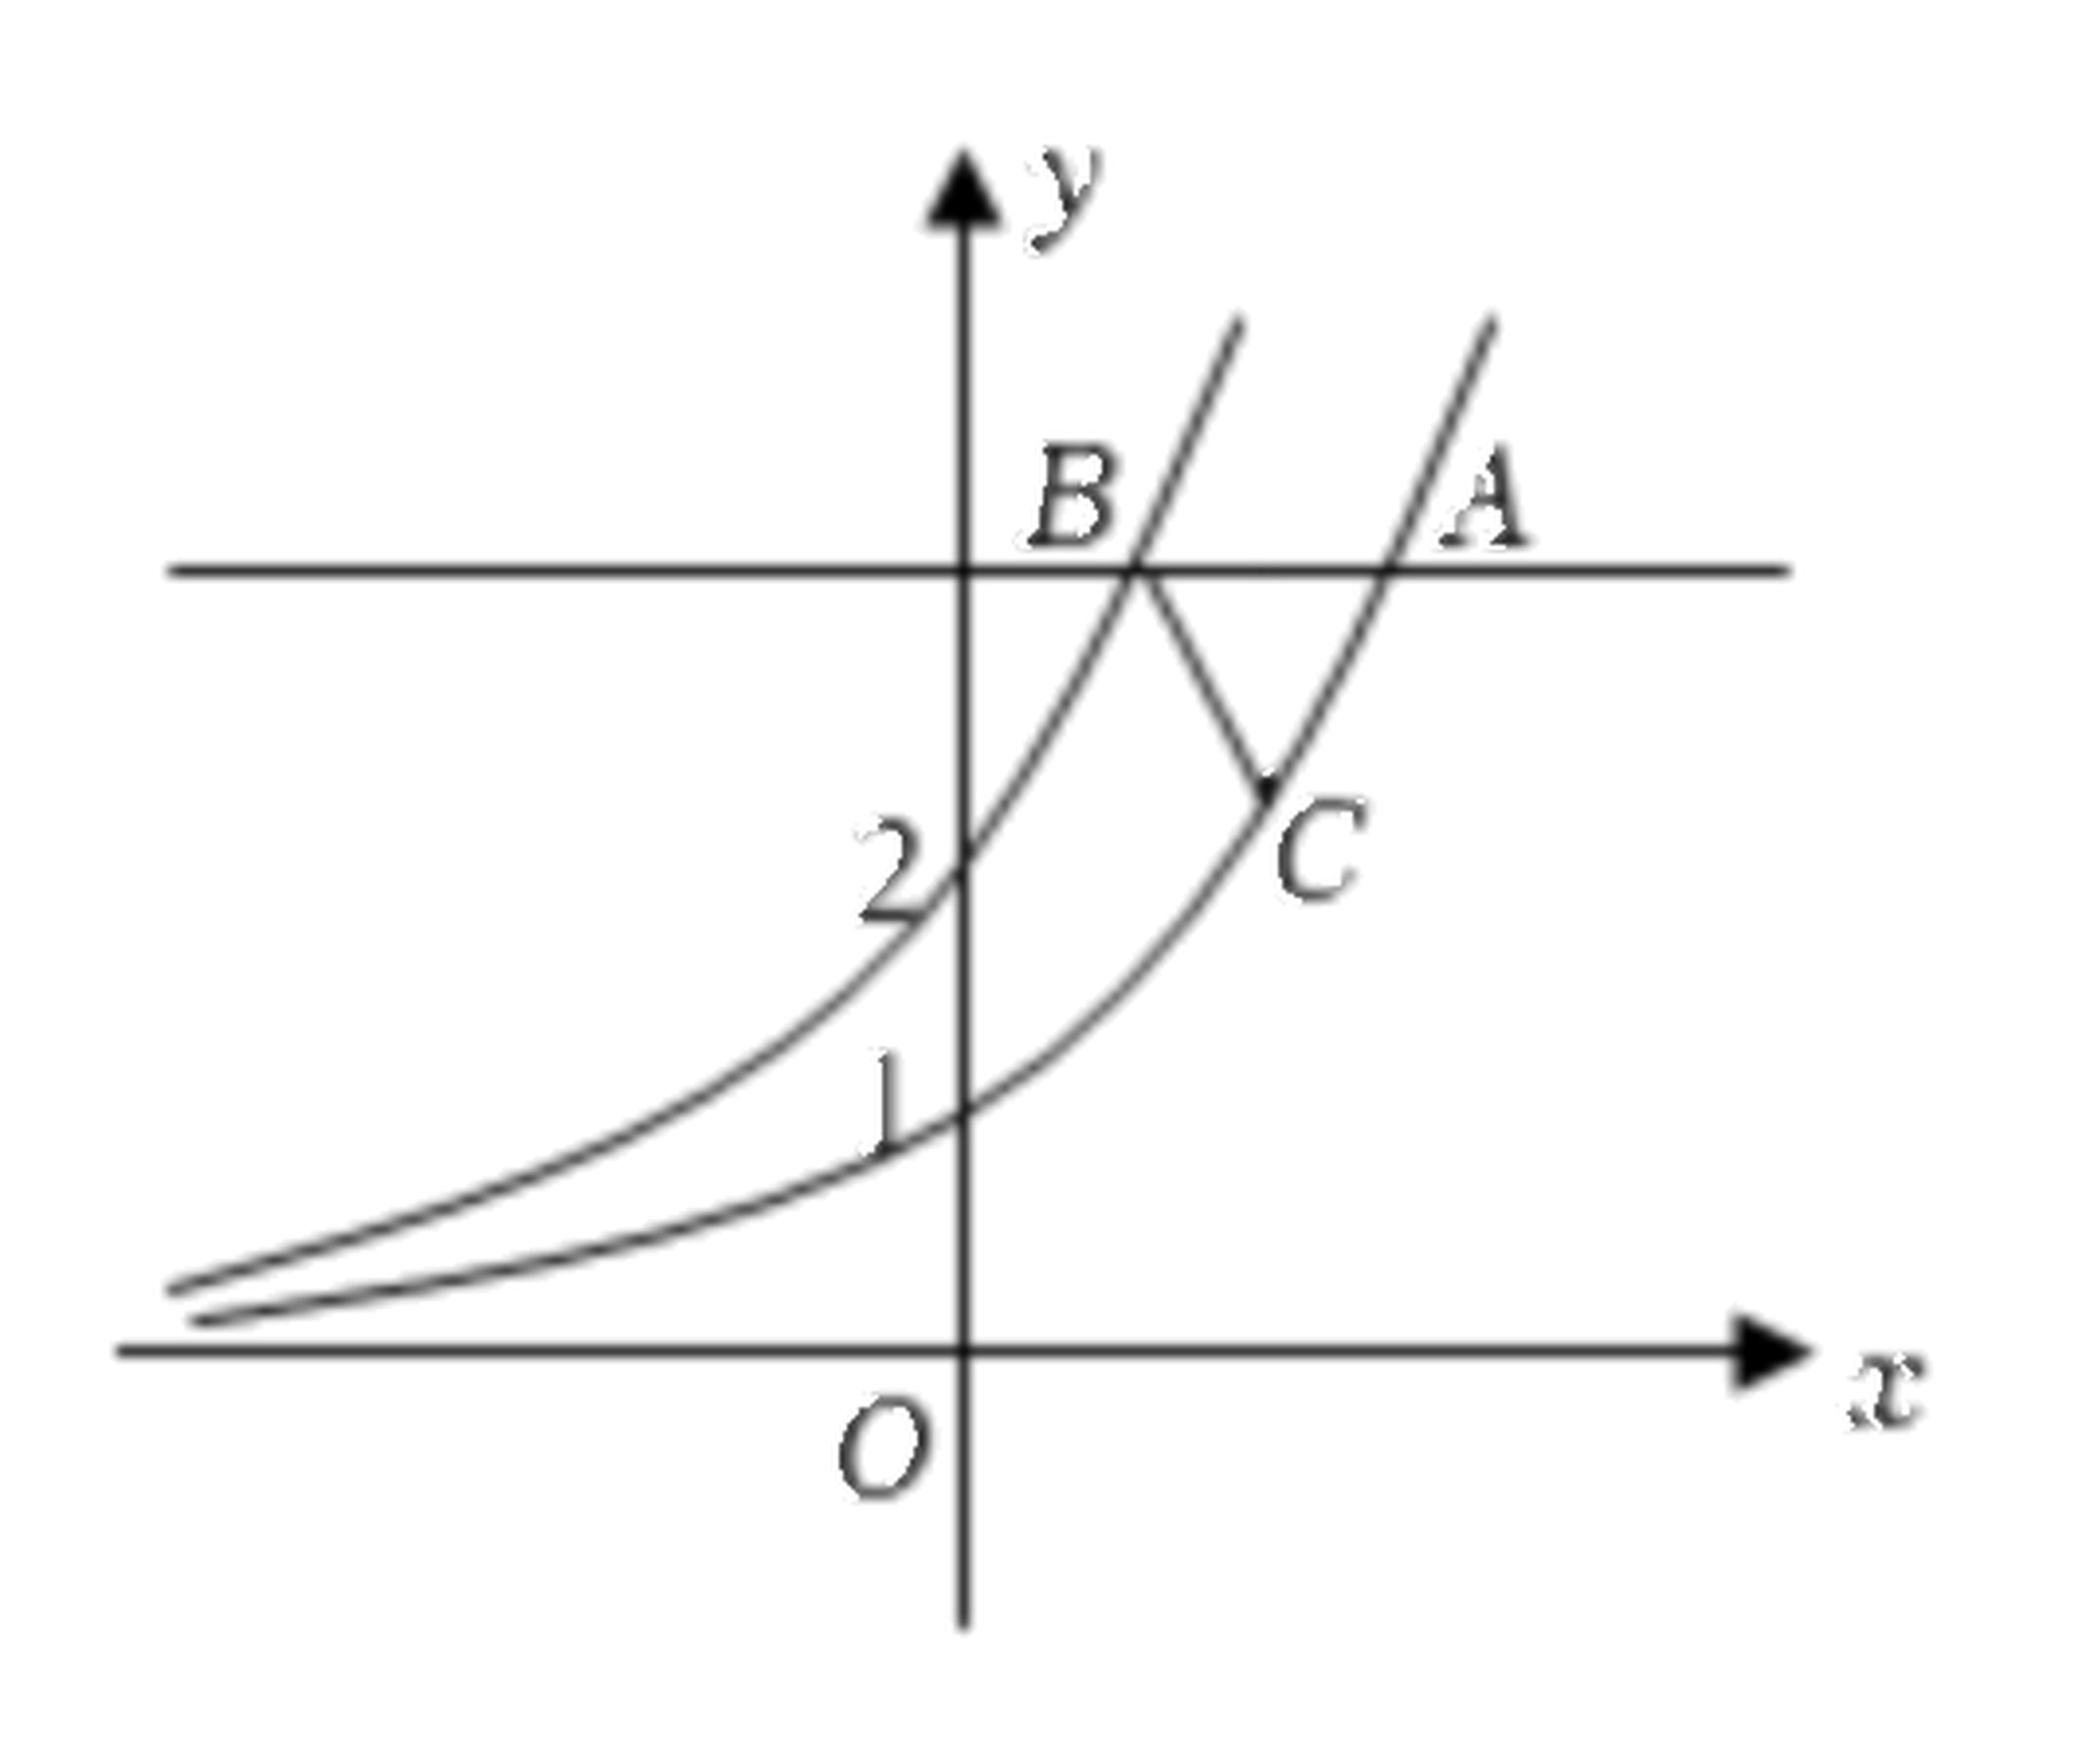
\includegraphics[width=0.40\textwidth]{figures/gao150_q11.png}
\end{center}

\ifanswer
\solbegin
\step{设直线 $l$ 的方程为 $y=a(a>0)$，}
\step{由 $2^x=a$，得 $x=\log_2 a$，所以 $A(\log_2 a,a)$，}
\step{由 $2^{x+1}=a$，得 $x=\log_2 a-1$，所以 $B(\log_2 a-1,a)$，所以 $\lvert AB\rvert=1$，}
\step{取 $AB$ 的中点 $D$，连接 $CD$，如图所示，}
\step{因为 $\triangle ABC$ 为等边三角形，则 $CD\perp AB$，且 $\lvert CD\rvert=\dfrac{\sqrt3}{2}$，}
\step{所以 $C\left(\log_2 a-\dfrac{1}{2},a-\dfrac{\sqrt3}{2}\right)$，}
\step{因为点 $C$ 在函数 $y=2^x$ 的图像上，所以 $a-\dfrac{\sqrt3}{2}=2^{\log_2 a-\frac{1}{2}}=\dfrac{a}{\sqrt2}$，}
\step{解得 $a=\dfrac{\sqrt3}{2-\sqrt2}=\dfrac{\sqrt3(2+\sqrt2)}{4-2}=\sqrt3+\dfrac{\sqrt6}{2}$，}
\step{所以点 $C$ 的纵坐标为 $a-\dfrac{\sqrt3}{2}=\dfrac{\sqrt3+\sqrt6}{2}$.}
\solend
\fi

% === Q12 === 解析配图（高斯函数方格阴影，仅答案版出）；"数学王子"弯引号；cases 块整体算一个印刷行；解析 4 行
\item 小玲在研究数学发展史，特别崇拜近代数学奠基者之一、享有“数学王子”称号的德国数学家高斯. 为了纪念高斯，我们把取整函数 $y=[x]$ 称为高斯函数，其中 $[x]$ 表示不超过 $x$ 的最大整数，如 $[1.1]=1$，$[-1.1]=-2$，则点集 $P=\{(x,y)\mid [x]^2+[y]^2=1\}$ 所表示的平面区域的面积为\blankline[4.4em].

\ifanswer
\solbegin
\step{$[x]^2+[y]^2=1$ 由 $\begin{cases}[x]=0\\ {[y]=-1}\end{cases}$ 或 $\begin{cases}[x]=0\\ {[y]=1}\end{cases}$ 或 $\begin{cases}[x]=-1\\ {[y]=0}\end{cases}$ 或 $\begin{cases}[x]=1\\ {[y]=0}\end{cases}$ 四个平面区域组成，}
\step{即 $\begin{cases}0\leqslant x<1\\ -1\leqslant y<0\end{cases}$ 或 $\begin{cases}0\leqslant x<1\\ 1\leqslant y<2\end{cases}$ 或 $\begin{cases}-1\leqslant x<0\\ 0\leqslant y<1\end{cases}$ 或 $\begin{cases}1\leqslant x<2\\ 0\leqslant y<1\end{cases}$，}
\step{作出平面区域如图所示，平面区域由四个边长为 $1$ 的正方形组成，}
\begin{center}
% 高斯函数 [x]^2+[y]^2=1 方格阴影区域图取 04 页顶部，去粉色水印、去色、4× LANCZOS 放大；仅答案版出
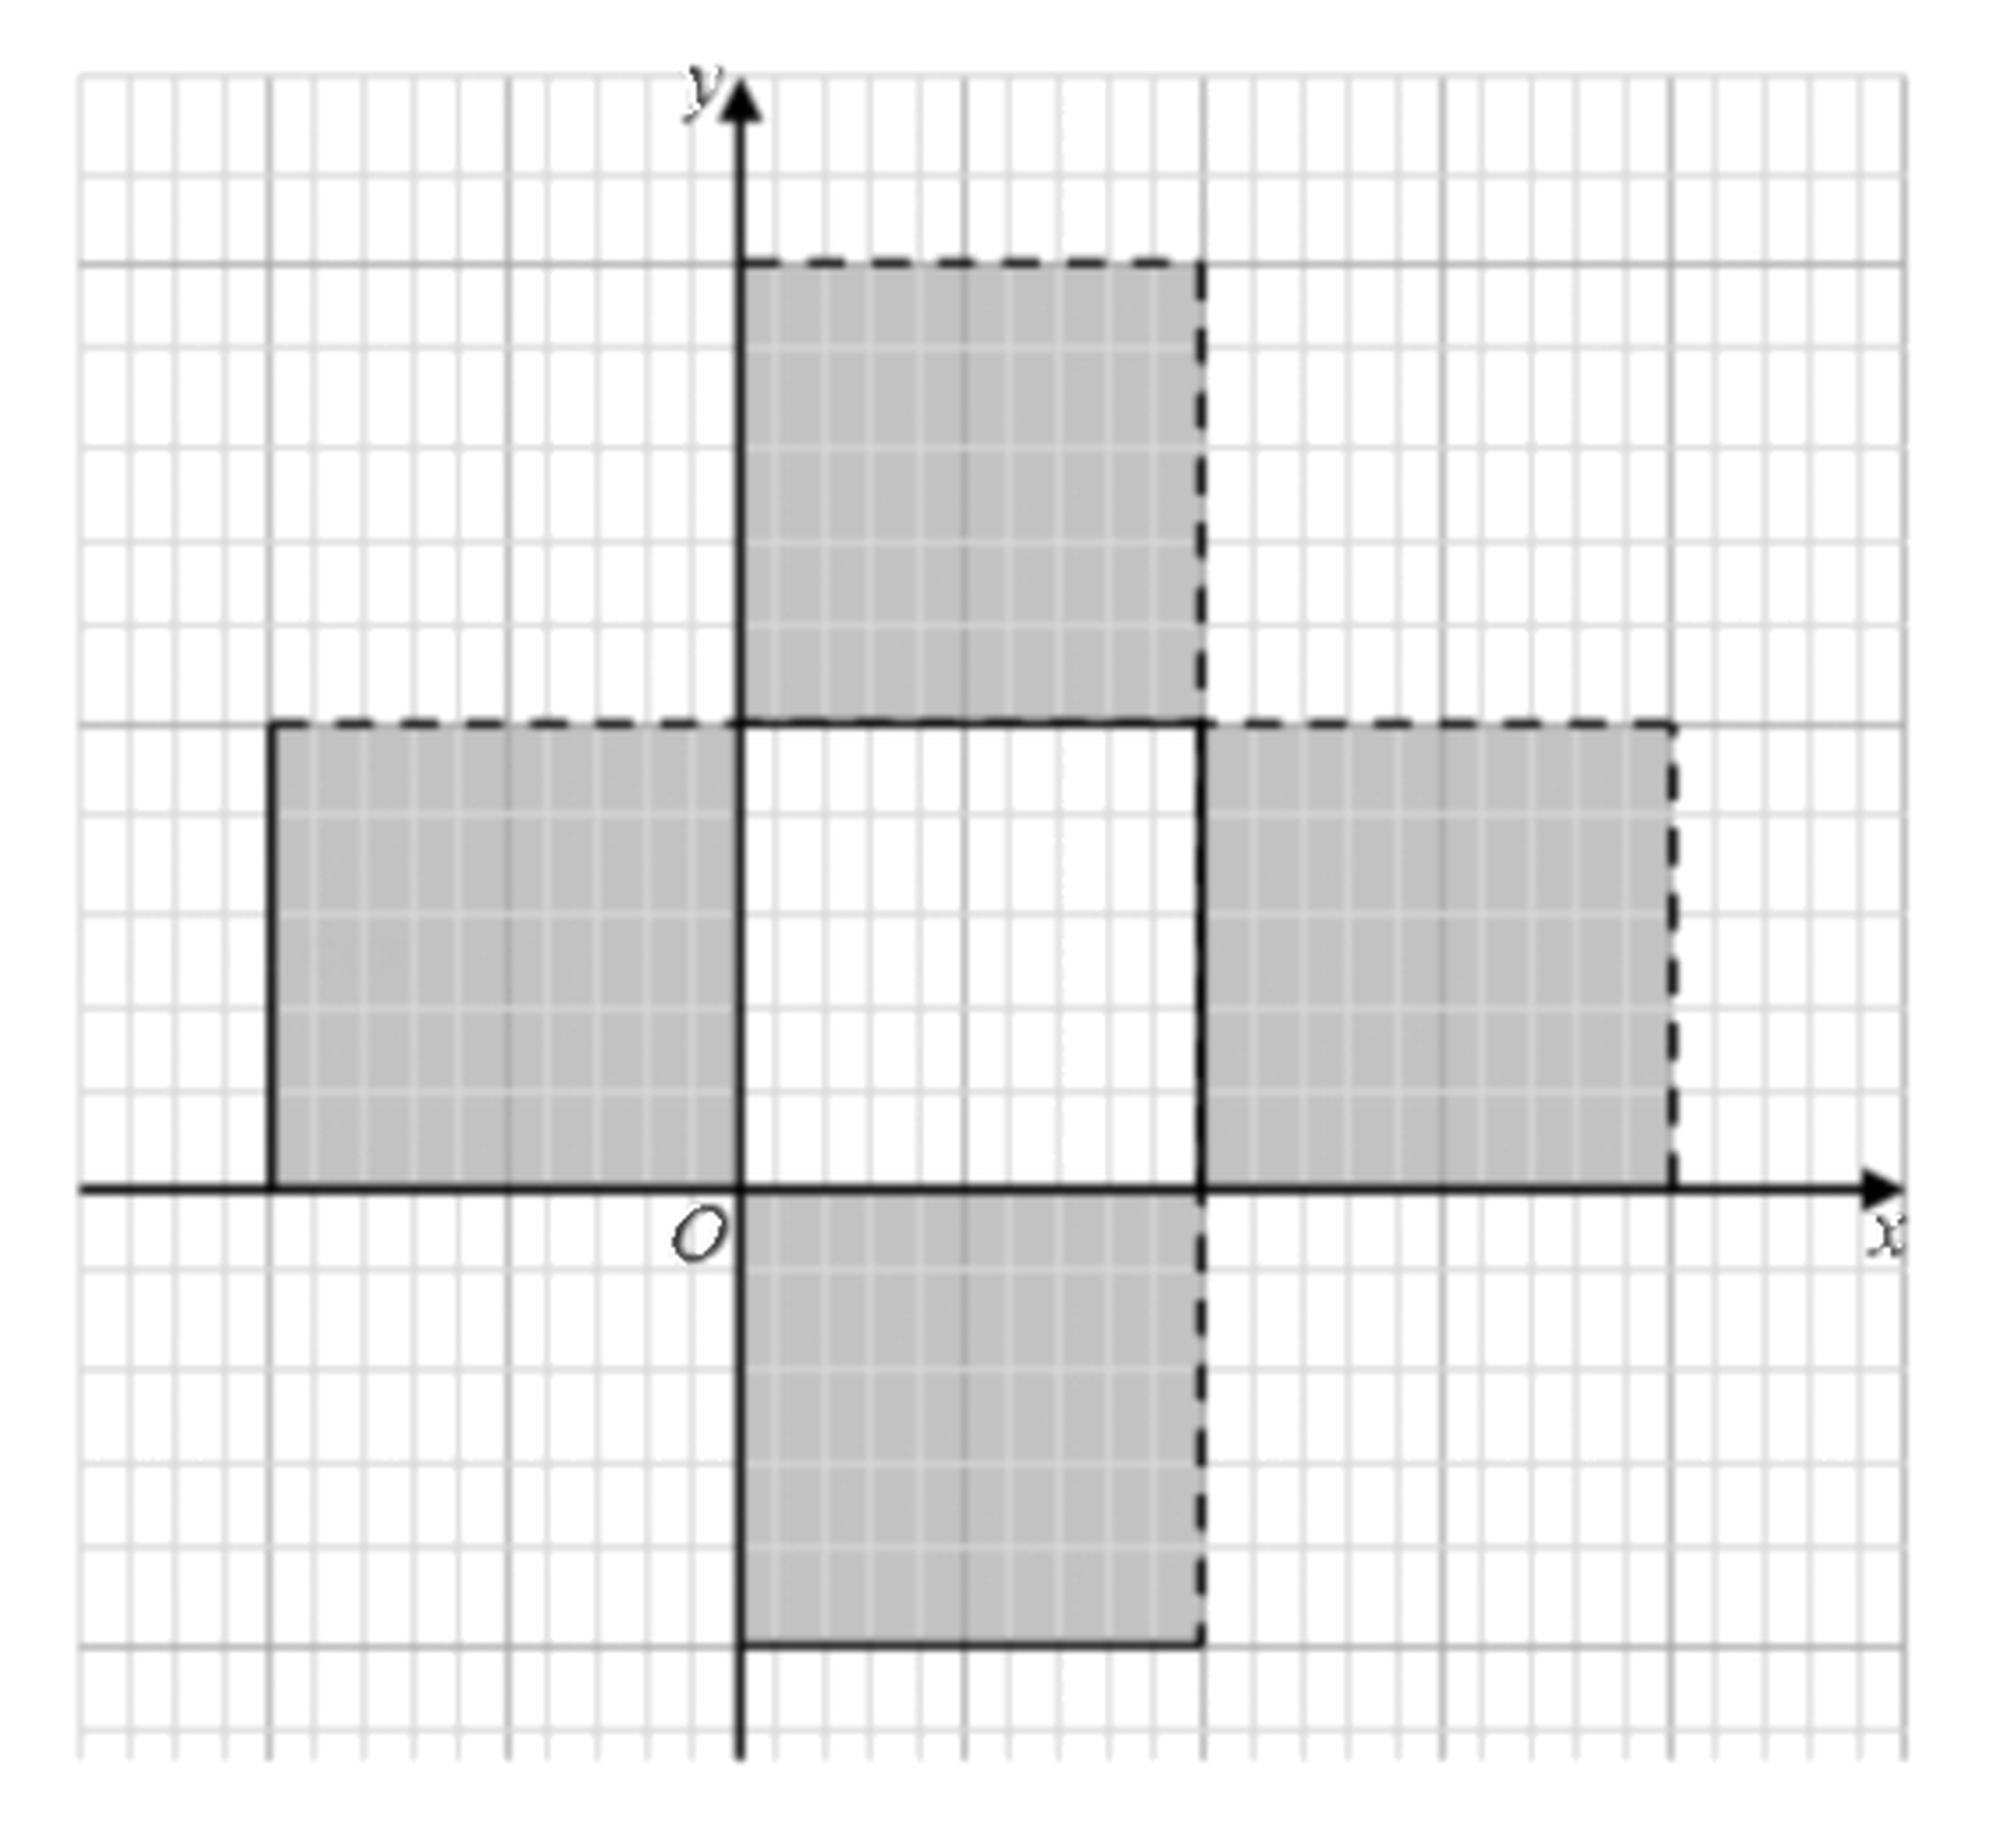
\includegraphics[width=0.34\textwidth]{figures/gao150_q12.png}
\end{center}
\step{总面积为 $1\times4=4$.}
\solend
\fi

\end{enumerate}

\bigsec{二、选择题}

\begin{enumerate}
\setcounter{enumi}{12}

% === Q13 === 答案在解析末句"故选 C"；括号 \mbox{（\quad）} 留空；四选项一行；解析 1 行
\item 设 $x\ne0$，则 $3^{\log_9 x^2}$ 的化简结果是\mbox{（\quad）}

\keepwithprev
A. $x$\qquad B. $\dfrac{1}{x}$\qquad C. $\lvert x\rvert$\qquad D. $\dfrac{1}{\lvert x\rvert}$

\ifanswer
\solbegin
\step{$3^{\log_9 x^2}=3^{\log_3\lvert x\rvert}=\lvert x\rvert$，故选 $C$.}
\solend
\fi

% === Q14 === 题目配图（两函数图像，三版都出）；\needvspace{8cm} 守卫放 \item 之前；"图像"照录；四选项两行两列；解析 2 行，故选 B
\needvspace{8cm}
\item 设 $a>0$ 且 $a\ne1$，$b\in\R$. 若函数 $y=a^{-\lvert x\rvert}$ 与 $y=x^b$ 的大致图像如图所示，则\mbox{（\quad）}

\keepwithprev
A. $0<a<1<b$\qquad\qquad B. $a>1$ 且 $b>1$

C. $0<a<1$ 且 $0<b<1$\qquad\qquad D. $0<b<1<a$

\begin{center}
% 两函数 y=a^{-|x|} 与 y=x^b 大致图像取 04 页右侧，去粉色水印、去色、4× LANCZOS 放大；三版都出
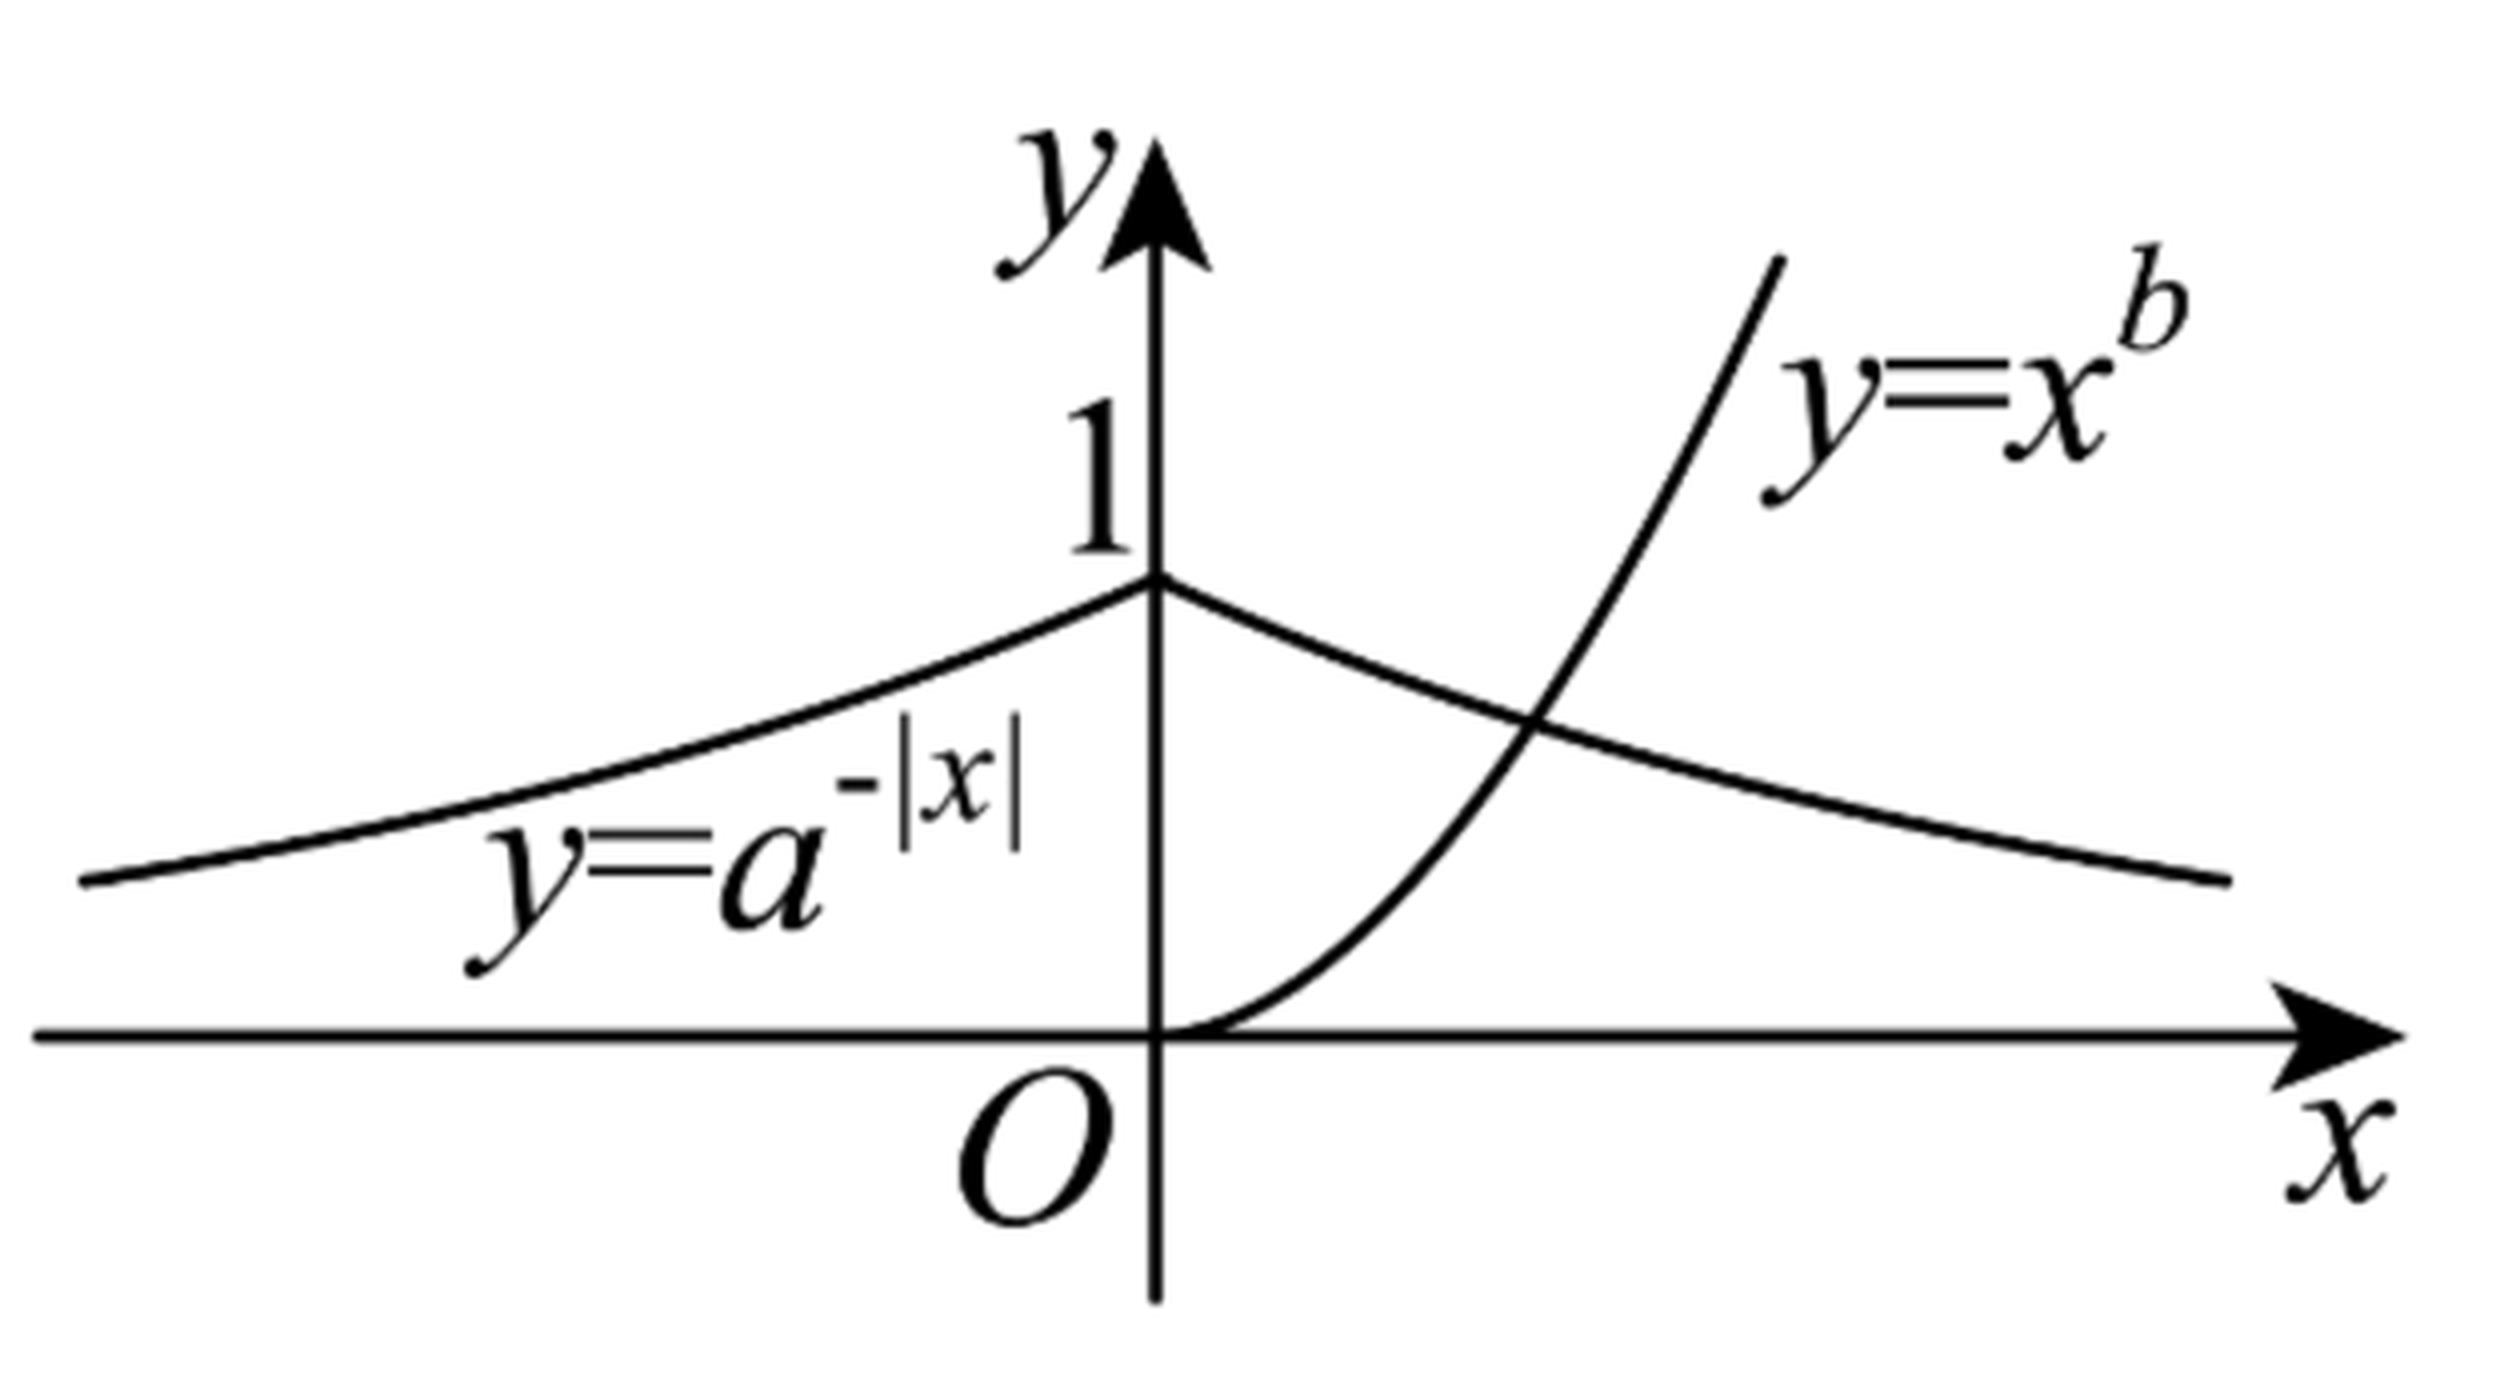
\includegraphics[width=0.40\textwidth]{figures/gao150_q14.png}
\end{center}

\ifanswer
\solbegin
\step{在 $(0,+\infty)$ 上，$y=a^{-x}$ 严格递减，得 $a>1$；}
\step{幂函数 $y=x^b$ 的图像递增且向上弯曲，得 $b>1$；故选 $B$.}
\solend
\fi

% === Q15 === "算术平均值／算术平均数"两处不同照录；四选项两行两列；解析 5 行（续 05 页顶），故选 B
\item 已知两个正数的算术平均值不小于它们的几何平均值，类比有以下结论：三个正数的算术平均数不小于它们的几何平均数，即当 $a,b,c$ 为正实数时，$\dfrac{a+b+c}{3}\geqslant\sqrt[3]{abc}$，当且仅当 $a=b=c$ 时等号成立. 利用上述结论，下列选项中判断正确的是\mbox{（\quad）}

\keepwithprev
A. 若 $x>0$，则 $2x+\dfrac{1}{x^2}\geqslant\dfrac{27}{8}$\qquad\qquad B. 若 $x>0$，则 $x^2+\dfrac{2}{x}\geqslant3$

C. 若 $0<x<1$，则 $x^2(1-x)\geqslant\dfrac{1}{9}$\qquad\qquad D. 若 $0<x<1$，则 $x^2(1-x)\leqslant\dfrac{1}{9}$

\ifanswer
\solbegin
\step{A：取 $x=1$，$2x+\dfrac{1}{x^2}=3<\dfrac{27}{8}$，错误.}
\step{B：$x^2+\dfrac{2}{x}=x^2+\dfrac{1}{x}+\dfrac{1}{x}\geqslant3\sqrt[3]{x^2\cdot\dfrac{1}{x}\cdot\dfrac{1}{x}}=3$，当且仅当 $x=1$ 时取等号，正确.}
\step{C：取 $x=\dfrac{1}{3}$，$x^2(1-x)=\dfrac{2}{27}<\dfrac{1}{9}$，错误.}
\step{D：取 $x=\dfrac{2}{3}$，$x^2(1-x)=\dfrac{4}{27}>\dfrac{1}{9}$，错误.}
\step{故选 $B$.}
\solend
\fi

% === Q16 === "完美集"新定义（弯引号、引号外空格照录）；圈数字①②文本模式；$n\in\N$；四选项两行两列；解析 9 行（6 行 05 页＋3 行 06 页顶），故选 A
\item 已知有限集 $A=\{a_1,a_2,\cdots,a_n\}$（$n\geqslant2$，$n\in\N$）. 若 $A$ 中元素 $a_i$（$i=1,2,\cdots,n$）满足 $a_1+a_2+\cdots+a_n=a_1\cdot a_2\cdots a_n$，就称 $A$ 为 “完美集”. 现有以下两个命题：

①恰有两个元素的 “完美集” 有无穷多个；

②若 $a_i$ 均为正整数，则 “完美集” $A$ 有且只有一个，且 $n=3$.

则\mbox{（\quad）}

\keepwithprev
A. ①和②都是真命题\qquad\qquad B. ①和②都是假命题

C. ①是真命题，②是假命题\qquad\qquad D. ①是假命题，②是真命题

\ifanswer
\solbegin
\step{①由 $a+b=ab\Leftrightarrow(a-1)(b-1)=1$，任取 $a>2$，则 $b=1+\dfrac{1}{a-1}\in(1,2)$，}
\step{得到无穷多个不同的完美集，①真.}
\step{②设 $1\leqslant a_1<a_2<\cdots<a_n$，则 $a_i\geqslant i$.}
\step{若 $n=2$，则 $(a_1-1)(a_2-1)=1$，只能有 $a_1=a_2=2$，与元素互异矛盾.}
\step{若 $n\geqslant4$，则 $a_1a_2\cdots a_n\geqslant a_2a_{n-1}a_n\geqslant2(n-1)a_n>na_n\geqslant a_1+\cdots+a_n$，矛盾.}
\step{当 $n=3$ 时，若 $a_1\geqslant2$，则 $a_1a_2a_3\geqslant6a_3>3a_3\geqslant a_1+a_2+a_3$，矛盾.}
\step{因此 $a_1=1$，$(a_2-1)(a_3-1)=2$，结合 $a_2<a_3$ 得 $a_2=2$，$a_3=3$.}
\step{唯一的完美集为 $\{1,2,3\}$，②真.}
\step{故选 $A$.}
\solend
\fi

\end{enumerate}

\bigsec{三、解答题}

\begin{enumerate}
\setcounter{enumi}{16}

% === Q17 === \varnothing 空集、$B\subseteq A$ 带下划线照录；弯引号内空格照录；解析 7 行
\item 设 $a,b\in\R$. 已知集合 $A=\{x\mid ax^2+3x-a>3\}$，$B=\{x\mid bx=1\}$.

(1) 若 $A=(1,2)$，求 $a$ 的值；

(2) 若 $a=0$，且 “ $x\in A$ ” 是 “ $x\in B$ ” 的必要非充分条件，求 $b$ 的取值范围.

\ifanswer
\solbegin
\step{(1) $A=(1,2)$，则 $a<0$，且 $1,2$ 是方程 $ax^2+3x-a-3=0$ 的两根.}
\step{由 $4a+6-a-3=0$，得 $a=-1$，此时不等式为 $-(x-1)(x-2)>0$，}
\step{解集确为 $(1,2)$.}
\step{(2) $a=0$ 时，$A=(1,+\infty)$，题意等价于 $B\subseteq A$ 且 $B\ne A$.}
\step{当 $b=0$ 时，$B=\varnothing$，符合条件.}
\step{当 $b\ne0$ 时，$B=\left\{\dfrac{1}{b}\right\}$，条件等价于 $\dfrac{1}{b}>1$，解得 $0<b<1$.}
\step{因此 $b$ 的取值范围为 $[0,1)$.}
\solend
\fi

% === Q18 === $p\in\Z$；"图像"（像，有亻）照录；指数 $-2p^2+5p$；解析 8 行（(1) 首行 06 页末＋2 行 07 页顶、(2) 5 行 07 页）
\item 设 $p\in\Z$，已知 $f(x)=x^{-2p^2+5p}$.

(1) 若幂函数 $y=f(x)$ 的图像关于原点成中心对称，且满足 $f(3)<f(4)$，求 $p$ 的值；

(2) 当 $p=-2$ 时，求满足 $f(2x+3)<f(x-4)$ 的 $x$ 的取值范围.

\ifanswer
\solbegin
\step{(1) 图像关于原点成中心对称，得整数 $-2p^2+5p$ 为奇数.}
\step{由 $f(3)<f(4)$，得 $-2p^2+5p>0\Leftrightarrow0<p<\dfrac{5}{2}$，}
\step{结合 $p\in\Z$，得 $p=1$ 或 $p=2$，对应指数分别为 $3$、$2$，所以 $p=1$.}
\step{(2) 当 $p=-2$ 时，$f(x)=\dfrac{1}{x^{18}}$，定义域为 $\{x\in\R\mid x\ne0\}$.}
\step{原不等式要求 $x\ne-\dfrac{3}{2}$ 且 $x\ne4$，}
\step{此时 $\dfrac{1}{(2x+3)^{18}}<\dfrac{1}{(x-4)^{18}}\Leftrightarrow\lvert 2x+3\rvert>\lvert x-4\rvert\Leftrightarrow(2x+3)^2>(x-4)^2$，}
\step{因此 $(x+7)(3x-1)>0\Leftrightarrow x<-7$ 或 $x>\dfrac{1}{3}$，}
\step{排除 $x=4$，得 $x\in(-\infty,-7)\cup\left(\dfrac{1}{3},4\right)\cup(4,+\infty)$.}
\solend
\fi

% === Q19 === $a\in\R$、$g(x)=f(2x+1)+a\cdot f(x)+2$；解析 6 行（(2) 末两行续 08 页顶）
\item 已知 $f(x)=2^x$.

(1) 求方程 $f(2x)-f(x)=6$ 的解；

(2) 设 $a\in\R$，$g(x)=f(2x+1)+a\cdot f(x)+2$，若对于任意 $x\in[-1,1]$，均有 $g(x)\geqslant1$，求 $a$ 的取值范围.

\ifanswer
\solbegin
\step{(1) 令 $t=2^x>0$，则 $t^2-t-6=(t-3)(t+2)=0$，}
\step{由 $t>0$ 得 $t=3$，所以 $x=\log_2 3$.}
\step{(2) 令 $t=2^x$，则 $t\in\left[\dfrac{1}{2},2\right]$，且 $g(x)\geqslant1\Leftrightarrow2t^2+at+1\geqslant0\Leftrightarrow a\geqslant-\left(2t+\dfrac{1}{t}\right)$，}
\step{由基本不等式得 $2t+\dfrac{1}{t}\geqslant2\sqrt{2t\cdot\dfrac{1}{t}}=2\sqrt2$，}
\step{当且仅当 $t=\dfrac{1}{\sqrt2}\in\left[\dfrac{1}{2},2\right]$ 时等号成立，}
\step{因此 $-\left(2t+\dfrac{1}{t}\right)$ 的最大值为 $-2\sqrt2$，所求范围为 $a\in[-2\sqrt2,+\infty)$.}
\solend
\fi

% === Q20 === "极闭集"新定义、3 问，全卷末题；$M\subseteq(0,+\infty)$ 带下划线照录；自定义运算 $x*y$ 星号照录；解析 13 行（9 行 08 页＋4 行 09 页上半）
\item 对于非空实数集 $M\subseteq(0,+\infty)$，若满足以下两个条件：

① $M$ 中至少含有 $2$ 个元素，且 $1\notin M$；

②对于 $M$ 中任意两个不相等的元素 $x$、$y$，定义 $x*y=\dfrac{xy+1}{x+y}$，且 $x*y\in M$.

则称 $M$ 为 “极闭集”.

(1) 分别判断集合 $A=\left\{\dfrac{1}{2},3\right\}$ 与集合 $B=(1,+\infty)$ 是否为 “极闭集” （无需理由）；

(2) 若 $M$ 是 “极闭集”，证明：$M$ 中不可能所有元素都小于 $1$；

(3) 证明：不存在任何有限集是 “极闭集”.

\ifanswer
\solbegin
\step{(1) $A$ 不是 “极闭集”，$B$ 是 “极闭集”.}
\step{(2) 假设 $M$ 中所有元素都小于 $1$，取其中两个不相等的元素 $x$、$y$，}
\step{则 $x*y-1=\dfrac{(1-x)(1-y)}{x+y}>0$，}
\step{这与 $x*y\in M$ 且 $M$ 中所有元素都小于 $1$ 矛盾.}
\step{(3) 假设有限集 $M$ 是 “极闭集”，}
\step{由 (2) 及 $1\notin M$，得 $M$ 中存在大于 $1$ 的元素.}
\step{若 $M$ 中有小于 $1$ 的元素，取其中最大的一个为 $a$，另取 $b\in M$ 且 $b>1$，}
\step{则 $a*b-a=\dfrac{1-a^2}{a+b}>0, a*b-1=\dfrac{(a-1)(b-1)}{a+b}<0$，}% 半角逗号在两个数学式组之间，全稿惯例、非笔误，照录
\step{于是 $a<a*b<1$ 且 $a*b\in M$，与 $a$ 的最大性矛盾.}
\step{若 $M$ 中没有小于 $1$ 的元素，则 $M\subseteq(1,+\infty)$.}
\step{取 $a=\min M$，另取 $b\in M$ 且 $b\ne a$，则 $a*b-a=\dfrac{1-a^2}{a+b}<0$，}
\step{于是 $a*b<a$ 且 $a*b\in M$，与 $a$ 的最小性矛盾.}
\step{因此不存在任何有限集是 “极闭集”.}
\solend
\fi

\end{enumerate}

\end{document}
"
% 紧凑版：xelatex "\def\iscompact{1}% 高一150_曹杨二中_期中.tex
%   —— 高一上数学"2026-2027 年曹杨二中高一上期中"（试卷版/答案版/紧凑版）
% 试卷版：xelatex 高一150_曹杨二中_期中.tex
% 答案版：xelatex "\def\isanswer{1}\input{高一150_曹杨二中_期中.tex}"
% 紧凑版：xelatex "\def\iscompact{1}\input{高一150_曹杨二中_期中.tex}"
%
% ① 原始材料：微信公众号"魔都数学加油站"文章，连载"27学年高一150"，原文标题
% "27学年高一150——2026-2027年上海市曹杨二中高一上期中"；
% 原文链接：https://mp.weixin.qq.com/s/xlQxmik8TZXR87RC6MnCrw 。
% 正文为 9 张 PNG 页（01/02/04/06/07/09 为 2560×3620，03/05/08 为 4762×6735，
% 同一篇各页分辨率混排，逐页按各自分辨率裁图核对，别按预览比例换算裁框）。
% 体例：讲评版——全 18 题均印【解析】（逐题核实，见 ② ②）。
% 题目、答案、解析均据原图转录；卷面粉红色/红色水印"魔都数学加油站"及公众号页脚未录入。
% 全卷插图清单（逐页通读 9 页确认）：3 幅——
%   · Q11 题目配图（指数函数曲线图，02 页右侧：x/y 轴、O、y=2^x 与 y=2^{x+1}
%     两曲线、A/B/C 三点、刻度 1/2、等边三角形 ABC），三版都出，裁 figures/gao150_q11.png；
%   · Q12 解析配图（高斯函数取整 [x]^2+[y]^2=1 方格阴影区域图，04 页顶部：4 个边长 1
%     的正方形组成的十字形阴影），解析"作出平面区域如图所示"处，仅答案版出，
%     放 \ifanswer 内 \step 之间，裁 figures/gao150_q12.png；
%   · Q14 题目配图（两函数 y=a^{-|x|} 与 y=x^b 大致图像，04 页右侧：x/y 轴、O、
%     y 轴刻度 1、一递减曲线一递增上翘曲线），三版都出，裁 figures/gao150_q14.png；
%   其余各页逐页确认无其它题目配图、无表格；Q11/Q12 解析"如图所示"对应的就是上列
%   已裁的图，不重复裁；09 页上半为 Q20(3) 解析续尾、下半仅水印、无正文。
%   3 图均取自原卷截图，去粉色水印、去色、4× LANCZOS 放大。
%
% 卷首标题：原卷印作"2026-2027 年曹杨二中高一上期中"，年份区间按全稿惯例排 en dash；
% 原卷卷面未印副标题，本稿按同期中卷知识模块口径补出"集合与常用逻辑用语、不等式、函数"。
%
% 题号体例（逐页核实定稿）：本卷共 18 题——一、填空题 3—12（10 题）、
% 二、选择题 13—16（4 题）、三、解答题 17—20（4 题）。
% 三节分别 \setcounter{enumi}{2}／{12}／{16}。原卷从第 3 题起、无第 1、2 题，
% 本稿保留原题号；全卷末题为第 20 题（"极闭集"新定义、3 问），无 Q21、无附加题节。
%
% ② 与原卷的排版差异：
%   ① 原文从第 3 题起，本稿保留原题号；共 18 题三节，解答题只有 4 题到 20；
%   ② 全 18 题均印【解析】，用 \solbegin…\solend；逐题核实无只印【答案】或
%      答案印题干括号内的题；四道选择题答案在解析末句"故选 X"（Q13 选 C、
%      Q14 选 B、Q15 选 B、Q16 选 A，逐个放大复核）、括号 \mbox{（\quad）} 留空、
%      不另提 \ans{}；答案版【答案】/【解析】标记数 = 18 = 全卷题数；
%   ③ 原卷卷面未印副标题，本稿按知识模块口径补出；
%   ④ 原卷填空横线按全稿惯例排 \blankline[4.4em]；选择题括号排 \mbox{（\quad）}、
%      选项段前按惯例加 \keepwithprev；解答题不留作答区、不加 \anspace（原卷为讲评版）；
%   ⑤ 数集黑板粗体：Q4"m\in R"、Q5"a,b\in R"、Q6"a,b,c\in R"、Q7"a\in R"、
%      Q10"a\in R"、Q14"b\in R"、Q17"a,b\in R"、Q18"p\in Z"／定义域"x\in R"、
%      Q19"a\in R"、Q16"n\in N" 原卷印斜体 R/Z/N，按全稿惯例归一 \R／\Z／\N；
%      绝对值排 \lvert…\rvert（Q7 |x+4|+|x-3|、Q11 |AB|／|CD|、Q13 |x|、
%      Q18 |2x+3|／|x-4|），集合描述竖线排 \mid（Q3、Q12、Q17、Q18、Q20），
%      不等号按全稿惯例排 \leqslant／\geqslant；补集照原卷上划线排 \overline{A}
%      （Q3 题干＋解析共 2 处）；空集符号 \varnothing（Q17 解析(2)）；
%      子集 \subset（单线⊂）／\subseteq（带下划线⊆）逐处照录，本卷 3 处子集
%      符号均印带下划线 ⊆、照录 \subseteq（Q20 题干、Q20 解析(3)、Q17 解析(2)，
%      见 ④），无 \subset 用例；
%   ⑥ 判别式 Δ/△：逐页通读 9 页，本卷无一元二次判别式算式，故无 Δ/△ 混用可照录
%      （"高 \Delta／扁 \triangle"口径备查，参照 高一142／144／145／146／148／149
%      头注④）；本卷仅 Q11 题干与解析共 2 处几何三角形符号 △ABC，逐处放大并排
%      确认两处同形、印近等边粗线三角（非判别式），照录 \triangle（见 ④）；
%   ⑦ 中文弯引号照录：Q12"数学王子"、Q16"完美集"（题干＋①②两命题，引号外
%      留空格）、Q17" x∈A "" x∈B "（引号内空格）、Q20"极闭集"（题干条件、
%      三问与解析，引号外留空格）；注释里一律 ASCII 引号；数学式内 CJK 用 \text{}
%      （Q3 集合描述"且"用 \text{ 且 }）；
%   ⑧ 半角逗号在数学组之间是全稿惯例、非笔误，逐处照录（Q17 解析"1,2 是方程…
%      两根"、Q20 解析(3)">0, a*b-1=…<0" 两式之间等）；行末西文句点 ASCII `.`；
%      行中全角逗号／顿号照录（Q12"之一、享有"、Q18 解析"3、2"、Q20"x、y"）；
%   ⑨ "图像／图象"逐处放大核：全卷 9 处均印"图像"（像，有亻）、未见"图象"——
%      Q4 题干 1、Q11 题干 2＋解析 1、Q14 题干 1＋解析 1、Q18 题干 1＋解析 1；
%      同卷"第二象限""象限"用"象"（无亻）。逐处照录未统一改动（放大 01/02/04/06
%      页 /tmp/gao150/z/p01_q4_tuxiang2.png、p04_q14_tuxiang2.png、
%      p02_q11_lines.png 确认）；子题标号 (1)(2)(3) 半角括号照录；圈数字①②
%      在文本模式（Q16 两命题与解析、Q20 两条件与三问及解析）按 common.sty
%      划入 CJK 字符类渲染，进数学式用 \text{①}；
%   ⑩ Q20 新定义 x*y=\dfrac{xy+1}{x+y} 的 * 是自定义运算（星号），照录；
%      \left…\right 不得拆到不同 $…$ 组（Q19"\left(2t+\frac1t\right)"、
%      Q20 题干"A=\left\{\frac12,3\right\}"等）；Q8 嵌套根号
%      \sqrt{\frac2x+\frac{16}{1-2x}}、Q9 对数连加 \log_2 A 等复杂式照录别简化；
%   ⑪ 一条 \step = 原卷解析的一个印刷行，cases 块整体算一个印刷行；别并折行、
%      别拆行。Q4 三行、Q8 五行、Q11 九行、Q12 四行（两行各含四个 cases 块）、
%      Q15 五行、Q16 九行、Q18 八行、Q20 十三行均按印刷行逐条断，不丢行；
%   ⑫ 配图：Q11／Q14 题目配图（三版都出）放 \item 内题干之后 \begin{center}，
%      大图块加 \needvspace{8cm} 守卫把整块推走（守卫放 \item 之前，见
%      高一145 Q14/Q20 成例与切页审计 B 类坑）；Q12 解析配图（仅答案版出）
%      放 \ifanswer 内 \solbegin…\solend 的 \step 之间（高一73 第16题成例）；
%   ⑬ 跨页续印按题合并：见 ⑥；
%   ⑭ 原卷解析内无红色"法一／法二"之类小标题，故本卷无 \stepm；红色水印
%      "魔都数学加油站"不录入；Q12 解析"作出平面区域如图所示"对应的图即
%      ① 所列 gao150_q12.png（04 页顶部），不重复裁；Q11 解析"如图所示"对应
%      题目配图 gao150_q11.png，不另裁。
%
% ③ 行数复核：一条 \step／\stepm = 原卷解析的一个印刷行，cases 块作一个印刷行计。
%   逐题数（主会话逐页核对定稿）：Q3：1；Q4：3；Q5：2；Q6：1；Q7：2；Q8：5；
%   Q9：1；Q10：3；Q11：9；Q12：4；Q13：1；Q14：2；Q15：5；Q16：9；
%   Q17：7；Q18：8；Q19：6；Q20：13。
%   合计 82 条 \step（本卷无 \stepm：解析内无红色"法一／法二"类小标题），
%   与原卷逐题印刷行相等。全卷 18 题均设 \solbegin…\solend，答案版
%   【答案】/【解析】标记数 = 18 = 全卷题数。
%
% ④ 判别式／三角形／子集符号结论（逐处放大原图照录、不得统一，主会话像素级复核）：
%   判别式：逐页通读 9 页，本卷无一元二次判别式 Δ/△ 算式（Q18 讨论幂函数指数
%     奇偶、不用判别式；Q9／Q19／Q20 亦无），头注 ② ⑥ 的"高 \Delta／扁 \triangle"
%     口径在本卷无对应处（参照 高一142／144／145／146／148／149 头注④，仅备查）。
%   几何三角形符号：Q11 题干"使得 △ABC 为等边三角形"（02 页末）与解析
%     "因为 △ABC 为等边三角形，则 CD⊥AB"（03 页）共 2 处，放大 02/03 页
%     /tmp/gao150/z/q11_tri_montage2.png 并排确认两处同形、印近等边粗线三角
%     （h/w≈0.98、非"高>宽"的判别式 \Delta），照录 \triangle（与 高一105
%     "使得 \triangle ABC 为等边三角形" 同短语成例、高一149 几何三角形照录
%     \triangle 口径一致），不引入 \Delta。
%   子集／补集：Q20 题干"$M\subseteq(0,+\infty)$"（08 页）、Q20 解析(3)
%     "则 $M\subseteq(1,+\infty)$"（09 页）、Q17 解析(2)"题意等价于 $B\subseteq A$
%     且 $B\ne A$"（06 页）共 3 处子集符号，逐处放大（/tmp/gao150/z/p08_q20_stem.png、
%     p09_q20_sub.png、p06_q17_sub.png）确认均印带下划线 ⊆，照录 \subseteq；
%     本卷未见单线 ⊂（\subset）之对应处。Q3 题干与解析共 2 处补集照原卷上划线
%     排 \overline{A}；Q17 解析(2) 空集印 ∅、照录 \varnothing（Q7"解集为空集"
%     为中文词、非符号，照录文字）；集合描述竖线 \mid；数集 \R／\Z／\N 归一见 ② ⑤。
%
% ⑤ 存疑照录（放大原图确认，照录未改、正文对应处另有 % 注）：
%   1. Q8 解析第 4 行"所以 $y=\frac1x+\frac{8}{1-2x}$ 的最小值为 18" —— 上文
%      并未定义 $y$，且题面求的是 $\sqrt{\frac2x+\frac{16}{1-2x}}$ 的最小值；
%      按上下文该行应为 $\frac1x+\frac{8}{1-2x}$ 的最小值为 18（$y$ 疑为原卷
%      衍字／笔误），放大 02 页 /tmp/gao150/z/p02_q8_y.png 确认，照录未改。
%   2. Q20 解析(3)"$a*b-a=\frac{1-a^2}{a+b}>0, a*b-1=\frac{(a-1)(b-1)}{a+b}<0$"
%      两式之间的逗号原卷印半角 ,（非全角），按全稿惯例"半角逗号在数学组之间"
%      照录未改（放大 08 页 /tmp/gao150/z/p08_q20_sol8.png 确认）。
%   3. Q15 题干"两个正数的算术平均值…几何平均值"与"三个正数的算术平均数…
%      几何平均数"两处"值／数"用字不同，逐处照录未统一（放大 04 页确认）。
%   4. "图像／图象"全卷 9 处均印"图像"（像，有亻）、未见"图象"，逐处放大核实
%      照录、未统一改动（见 ② ⑨）；本卷判别式 Δ/△ 无用例、几何三角形 2 处
%      照录 \triangle（见 ④）。
%   全卷除此 4 类外未发现其它笔误／自相矛盾处；18 题均印【解析】、无只印【答案】
%   或答案印题干括号内的题（见 ② ②）。
%
% ⑥ 跨页续印按题合并说明（逐页核实定稿）：Q3/4/5/6/7 题干＋解析在 01 页；
%   Q8 题干＋解析 5 行、Q9 题干＋解析 1 行在 02 页上半；Q10 题干＋解析 3 行
%   在 02 页下半；Q11 题干（前两行）＋配图在 02 页下半、题干续"三角形，则点 C
%   的纵坐标为___"与解析 9 行全在 03 页上半（解析"如图所示"对应题目配图）；
%   Q12 题干＋解析 4 行在 03 页下半，解析配图（方格阴影）续印在 04 页顶部；
%   "二、选择题"标题在 04 页中部；Q13 题干＋选项＋解析、Q14 题干＋选项＋
%   配图＋解析在 04 页；Q15 题干＋四选项在 04 页末、解析 5 行续 05 页上半；
%   Q16 题干＋①②两命题＋"则(  )"＋四选项＋解析前 6 行在 05 页、解析末 3 行
%   （"因此 a_1=1…②真""故选 A"）续 06 页顶部；"三、解答题"标题在 06 页；
%   Q17 题干(1)(2)＋解析(1) 3 行＋解析(2) 首行在 06 页、解析(2) 续 3 行
%   在 06 页下半；Q18 题干(1)(2)＋解析(1) 首行在 06 页末、解析(1) 续 2 行＋
%   解析(2) 5 行在 07 页上半；Q19 题干(1)(2)＋解析(1) 2 行＋解析(2) 前 2 行
%   在 07 页下半、解析(2) 末 2 行续 08 页顶部；Q20 题干（新定义＋①②两条件）
%   ＋三问＋解析(1)(2)(3) 前 9 行在 08 页、解析(3) 末 4 行续 09 页上半，
%   末行"因此不存在任何有限集是极闭集"为全卷收尾（09 页下半仅水印、无正文）。
%   本稿按题连排，不丢行、不并折行；全卷末题为第 20 题，无 Q21、无附加题节。
%
\documentclass[a4paper,11pt]{article}
\usepackage{common}

\begin{document}

\examtitlest[3]{2026--2027 年曹杨二中高一上期中}{集合与常用逻辑用语、不等式、函数}

\bigsec{一、填空题}

\begin{enumerate}
\setcounter{enumi}{2}

% === Q3 === 补集上划线 \overline{A}（题干＋解析各 1 处）；集合描述竖线 \mid、数学式内"且"用 \text{}；解析 1 行
\item 设全集 $U=\{1,2,3,4,5\}$，集合 $A=\{x\mid x^2-3x\leqslant0\text{ 且 }x\in U\}$，则 $\overline{A}=$\blankline[4.4em].

\ifanswer
\solbegin
\step{$x^2-3x\leqslant0\Leftrightarrow0\leqslant x\leqslant3$，所以 $A=\{1,2,3\}$，$\overline{A}=\{4,5\}$.}
\solend
\fi

% === Q4 === "图像"（像，有亻）逐处照录、同句"第二象限"用"象"（无亻）；解析 3 行
\item 设 $m\in\R$. 若幂函数 $y=(m^2-5m+1)x^{m+1}$ 的图像经过第二象限，则 $m=$\blankline[4.4em].

\ifanswer
\solbegin
\step{幂函数的系数为 1，故 $m^2-5m+1=1\Rightarrow m=0$ 或 $m=5$.}
\step{$m=0$ 时，$y=x$ 不经过第二象限；}
\step{$m=5$ 时，$y=x^6$ 经过第二象限，因此 $m=5$.}
\solend
\fi

% === Q5 === 解析 2 行
\item 设 $a,b\in\R$. 若 $a^2+\dfrac{b^2}{4}=1$，则 $ab$ 的最大值为\blankline[4.4em].

\ifanswer
\solbegin
\step{$1-ab=\left(a-\dfrac{b}{2}\right)^2\geqslant0$，即 $ab\leqslant1$；}
\step{当 $a=\dfrac{\sqrt2}{2}$，$b=\sqrt2$ 时取等号，最大值为 1.}
\solend
\fi

% === Q6 === 解析 1 行
\item 设 $a,b,c\in\R$. 若等式 $2x^2-3x-2=a(x-1)^2+b(x-1)+c$ 恒成立，则 $a-b+c=$\blankline[4.4em].

\ifanswer
\solbegin
\step{令 $x=0$，得 $a-b+c=-2$.}
\solend
\fi

% === Q7 === 绝对值 \lvert…\rvert；解析 2 行
\item 设 $a\in\R$. 若关于 $x$ 的不等式 $\lvert x+4\rvert+\lvert x-3\rvert<a$ 的解集为空集，则 $a$ 的取值范围是\blankline[4.4em].

\ifanswer
\solbegin
\step{$\lvert x+4\rvert+\lvert x-3\rvert\geqslant\lvert(x+4)-(x-3)\rvert=7$，当 $-4\leqslant x\leqslant3$ 时取等号.}
\step{原不等式的解集为空集当且仅当 $a\leqslant7$，即 $a\in(-\infty,7]$.}
\solend
\fi

% === Q8 === 嵌套根号 \sqrt{\frac{2}{x}+\frac{16}{1-2x}} 照录别简化；解析 5 行
\item 设 $x\in\left(0,\dfrac{1}{2}\right)$，则 $\sqrt{\dfrac{2}{x}+\dfrac{16}{1-2x}}$ 的最小值为\blankline[4.4em].

\ifanswer
\solbegin
\step{因为 $x\in\left(0,\dfrac{1}{2}\right)$，所以 $1-2x>0$，又 $2x+1-2x=1$，}
\step{所以 $\left(\dfrac{1}{x}+\dfrac{8}{1-2x}\right)(2x+1-2x)=10+\dfrac{1-2x}{x}+\dfrac{16x}{1-2x}$}
\step{$\geqslant10+2\sqrt{\dfrac{1-2x}{x}\cdot\dfrac{16x}{1-2x}}=18$，}
\step{当且仅当 $\dfrac{1-2x}{x}=\dfrac{16x}{1-2x}$ 即 $x=\dfrac{1}{6}$ 时取等号，所以 $y=\dfrac{1}{x}+\dfrac{8}{1-2x}$ 的最小值为 18，}% 原卷此处径写 $y=\frac1x+\frac{8}{1-2x}$（上文未定义 $y$、且与题面根式不符），疑笔误，放大 02 页确认，照录未改（见 ⑤）
\step{所以 $\sqrt{\dfrac{2}{x}+\dfrac{16}{1-2x}}$ 的最小值为 6.}
\solend
\fi

% === Q9 === 对数连加 \log_2 A 等复杂式照录别简化；解析 1 行
\item 记 $A=1\times2\times3\times\cdots\times2026$，则 $\dfrac{1}{\log_2 A}+\dfrac{1}{\log_3 A}+\dfrac{1}{\log_4 A}+\cdots+\dfrac{1}{\log_{2026}A}=$\blankline[4.4em].

\ifanswer
\solbegin
\step{原式 $=\log_A 2+\cdots+\log_A 2026=\log_A(2\times3\times\cdots\times2026)=\log_A A=1$.}
\solend
\fi

% === Q10 === "严格减函数／不恒为负／⇔"照录；解析 3 行
\item 设 $a\in\R$，$f(x)=\dfrac{ax+1}{x+2}$. 若函数 $y=f(x)$ 在 $[1,+\infty)$ 上是严格减函数，且在 $[1,+\infty)$ 上的函数值不恒为负，则 $a$ 的取值范围是\blankline[4.4em].

\ifanswer
\solbegin
\step{当 $1\leqslant x_1<x_2$ 时，$f(x_2)-f(x_1)=\dfrac{(2a-1)(x_2-x_1)}{(x_1+2)(x_2+2)}$，故严格递减 $\Leftrightarrow a<\dfrac{1}{2}$.}
\step{此时最大函数值为 $f(1)$，函数值不恒为负 $\Leftrightarrow f(1)=\dfrac{a+1}{3}\geqslant0\Leftrightarrow a\geqslant-1$，}
\step{得 $a\in\left[-1,\dfrac{1}{2}\right)$.}
\solend
\fi

% === Q11 === 题目配图（指数函数曲线，三版都出）；\needvspace{8cm} 守卫放 \item 之前；"图像"照录、几何三角形 \triangle；解析 9 行（全在 03 页）
\needvspace{8cm}
\item 如图，点 $C$ 是函数 $y=2^x$ 的图像上的一点，若存在平行于 $x$ 轴的直线 $l$ 分别与函数 $y=2^x$ 和 $y=2^{x+1}$ 的图像相交于点 $A$、$B$，使得 $\triangle ABC$ 为等边三角形，则点 $C$ 的纵坐标为\blankline[4.4em].

\begin{center}
% 指数函数曲线图取 02 页右侧，去粉色水印、去色、4× LANCZOS 放大；三版都出
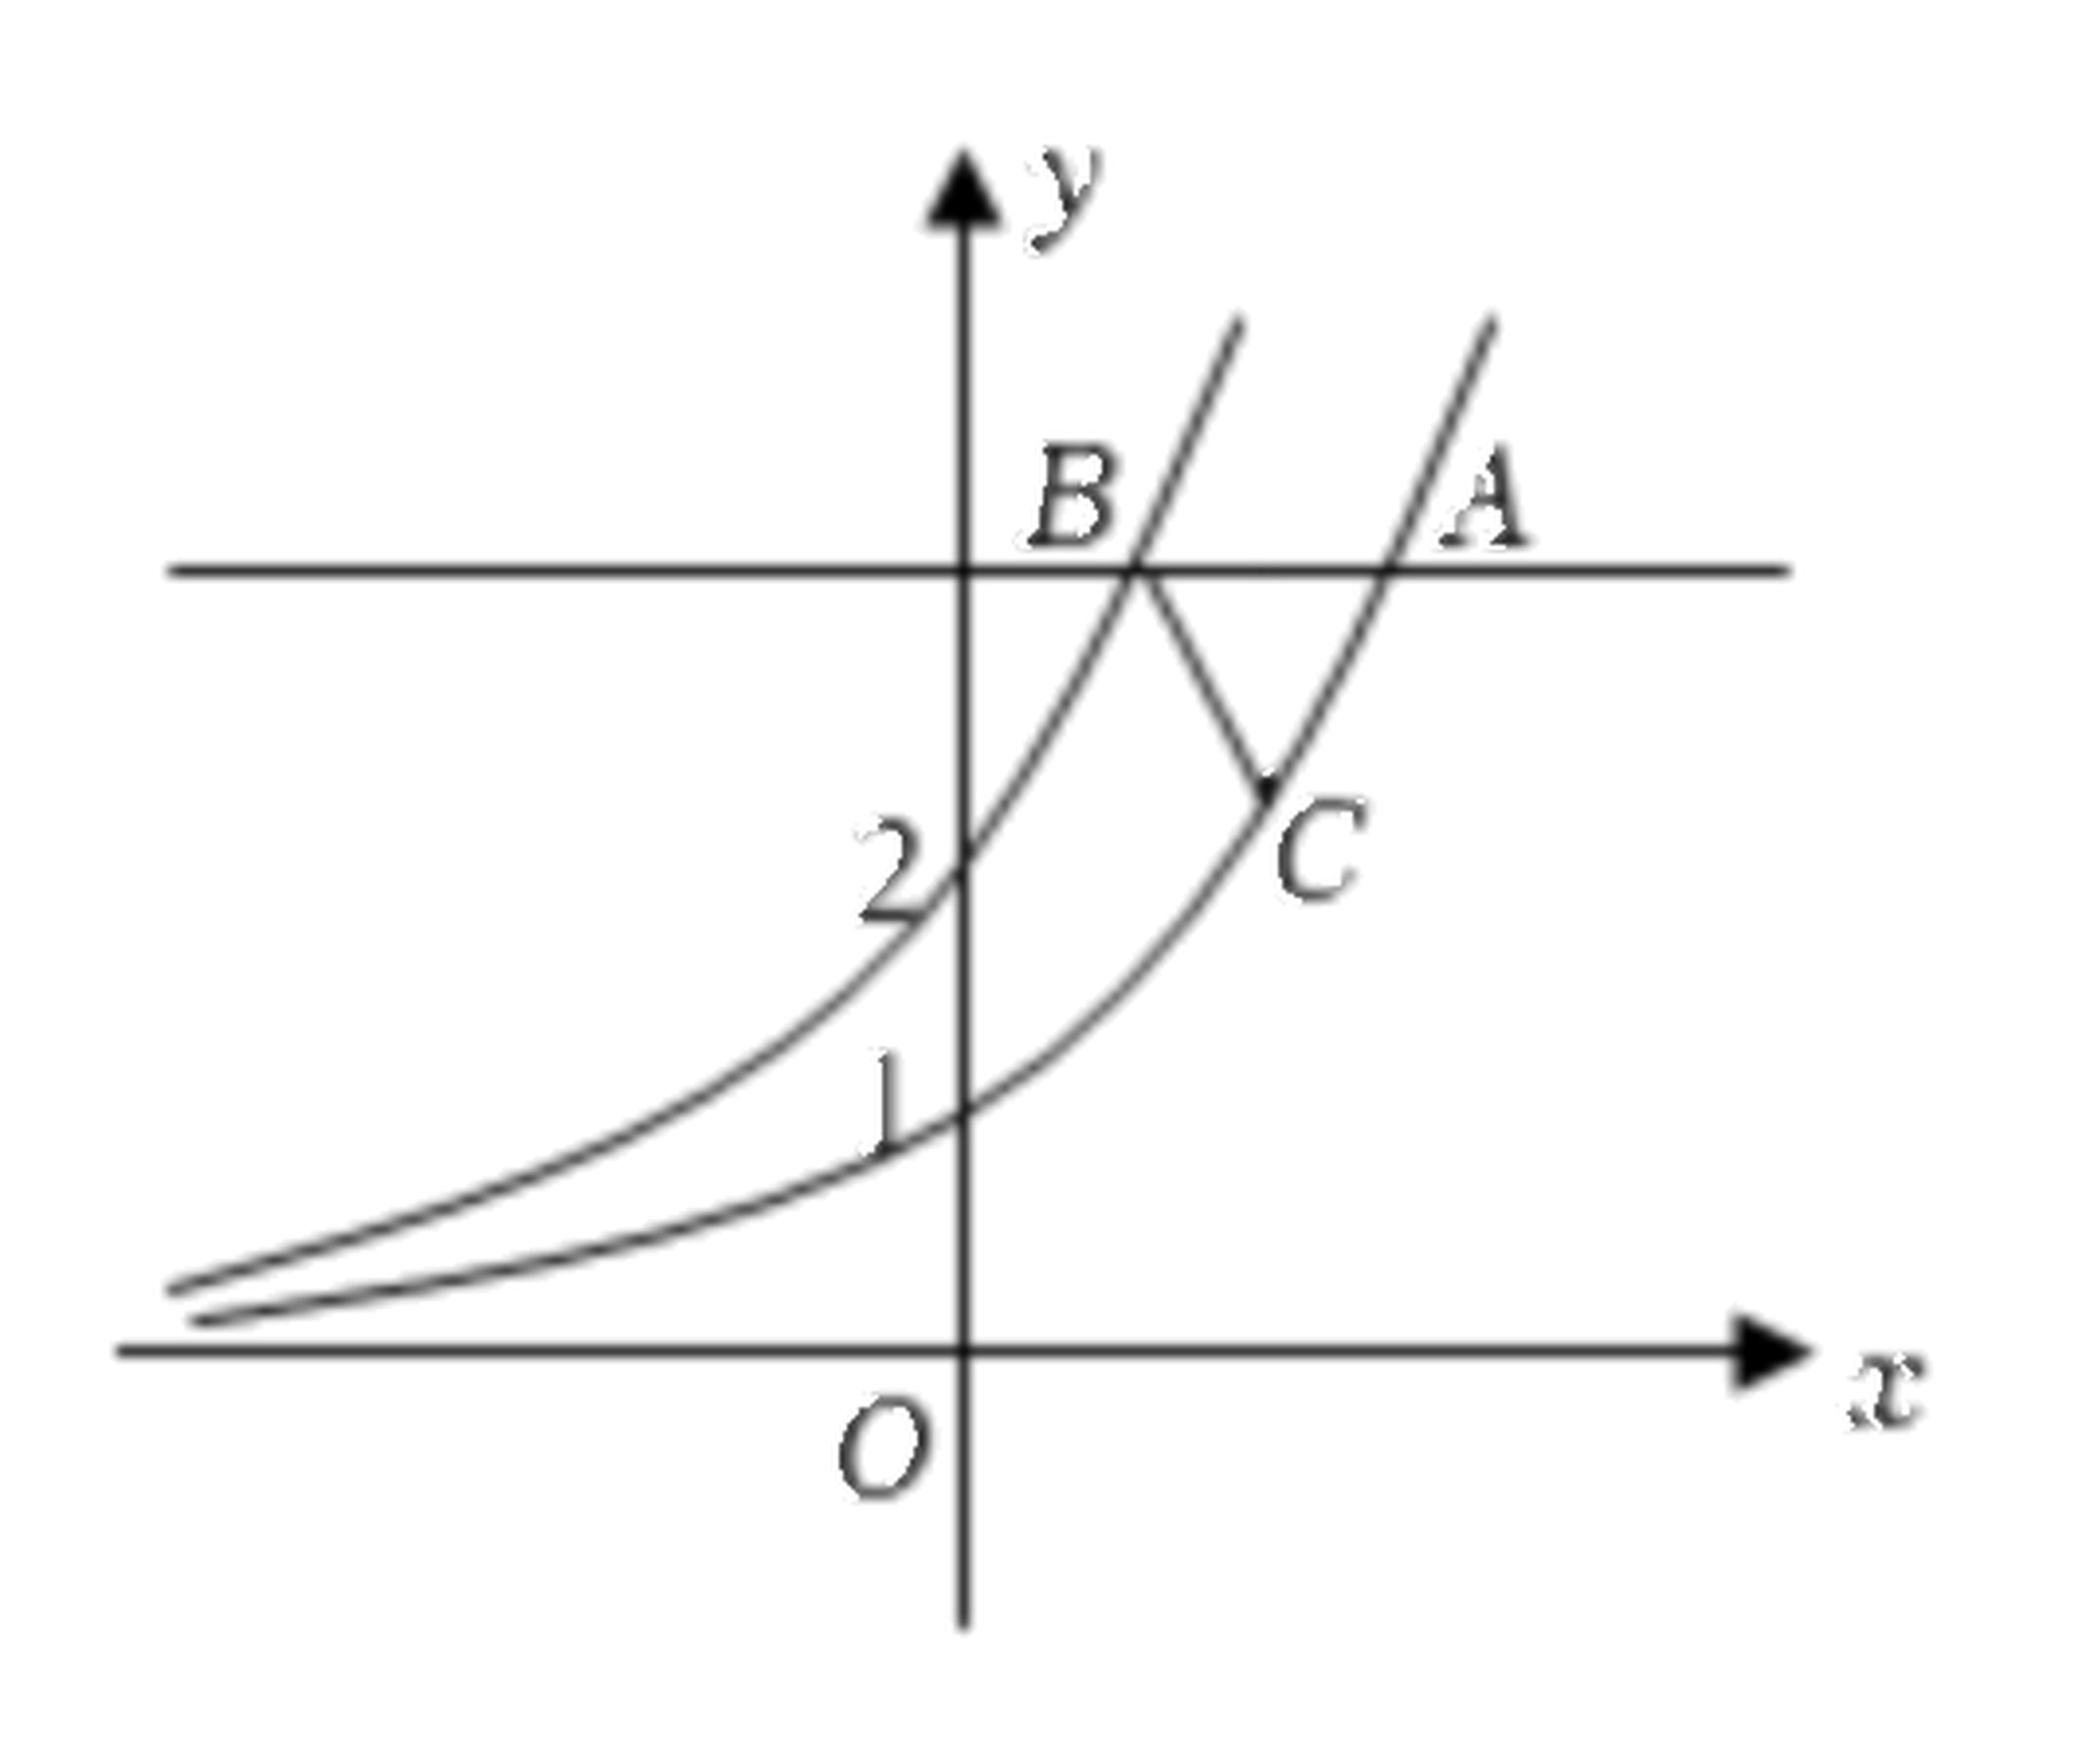
\includegraphics[width=0.40\textwidth]{figures/gao150_q11.png}
\end{center}

\ifanswer
\solbegin
\step{设直线 $l$ 的方程为 $y=a(a>0)$，}
\step{由 $2^x=a$，得 $x=\log_2 a$，所以 $A(\log_2 a,a)$，}
\step{由 $2^{x+1}=a$，得 $x=\log_2 a-1$，所以 $B(\log_2 a-1,a)$，所以 $\lvert AB\rvert=1$，}
\step{取 $AB$ 的中点 $D$，连接 $CD$，如图所示，}
\step{因为 $\triangle ABC$ 为等边三角形，则 $CD\perp AB$，且 $\lvert CD\rvert=\dfrac{\sqrt3}{2}$，}
\step{所以 $C\left(\log_2 a-\dfrac{1}{2},a-\dfrac{\sqrt3}{2}\right)$，}
\step{因为点 $C$ 在函数 $y=2^x$ 的图像上，所以 $a-\dfrac{\sqrt3}{2}=2^{\log_2 a-\frac{1}{2}}=\dfrac{a}{\sqrt2}$，}
\step{解得 $a=\dfrac{\sqrt3}{2-\sqrt2}=\dfrac{\sqrt3(2+\sqrt2)}{4-2}=\sqrt3+\dfrac{\sqrt6}{2}$，}
\step{所以点 $C$ 的纵坐标为 $a-\dfrac{\sqrt3}{2}=\dfrac{\sqrt3+\sqrt6}{2}$.}
\solend
\fi

% === Q12 === 解析配图（高斯函数方格阴影，仅答案版出）；"数学王子"弯引号；cases 块整体算一个印刷行；解析 4 行
\item 小玲在研究数学发展史，特别崇拜近代数学奠基者之一、享有“数学王子”称号的德国数学家高斯. 为了纪念高斯，我们把取整函数 $y=[x]$ 称为高斯函数，其中 $[x]$ 表示不超过 $x$ 的最大整数，如 $[1.1]=1$，$[-1.1]=-2$，则点集 $P=\{(x,y)\mid [x]^2+[y]^2=1\}$ 所表示的平面区域的面积为\blankline[4.4em].

\ifanswer
\solbegin
\step{$[x]^2+[y]^2=1$ 由 $\begin{cases}[x]=0\\ {[y]=-1}\end{cases}$ 或 $\begin{cases}[x]=0\\ {[y]=1}\end{cases}$ 或 $\begin{cases}[x]=-1\\ {[y]=0}\end{cases}$ 或 $\begin{cases}[x]=1\\ {[y]=0}\end{cases}$ 四个平面区域组成，}
\step{即 $\begin{cases}0\leqslant x<1\\ -1\leqslant y<0\end{cases}$ 或 $\begin{cases}0\leqslant x<1\\ 1\leqslant y<2\end{cases}$ 或 $\begin{cases}-1\leqslant x<0\\ 0\leqslant y<1\end{cases}$ 或 $\begin{cases}1\leqslant x<2\\ 0\leqslant y<1\end{cases}$，}
\step{作出平面区域如图所示，平面区域由四个边长为 $1$ 的正方形组成，}
\begin{center}
% 高斯函数 [x]^2+[y]^2=1 方格阴影区域图取 04 页顶部，去粉色水印、去色、4× LANCZOS 放大；仅答案版出
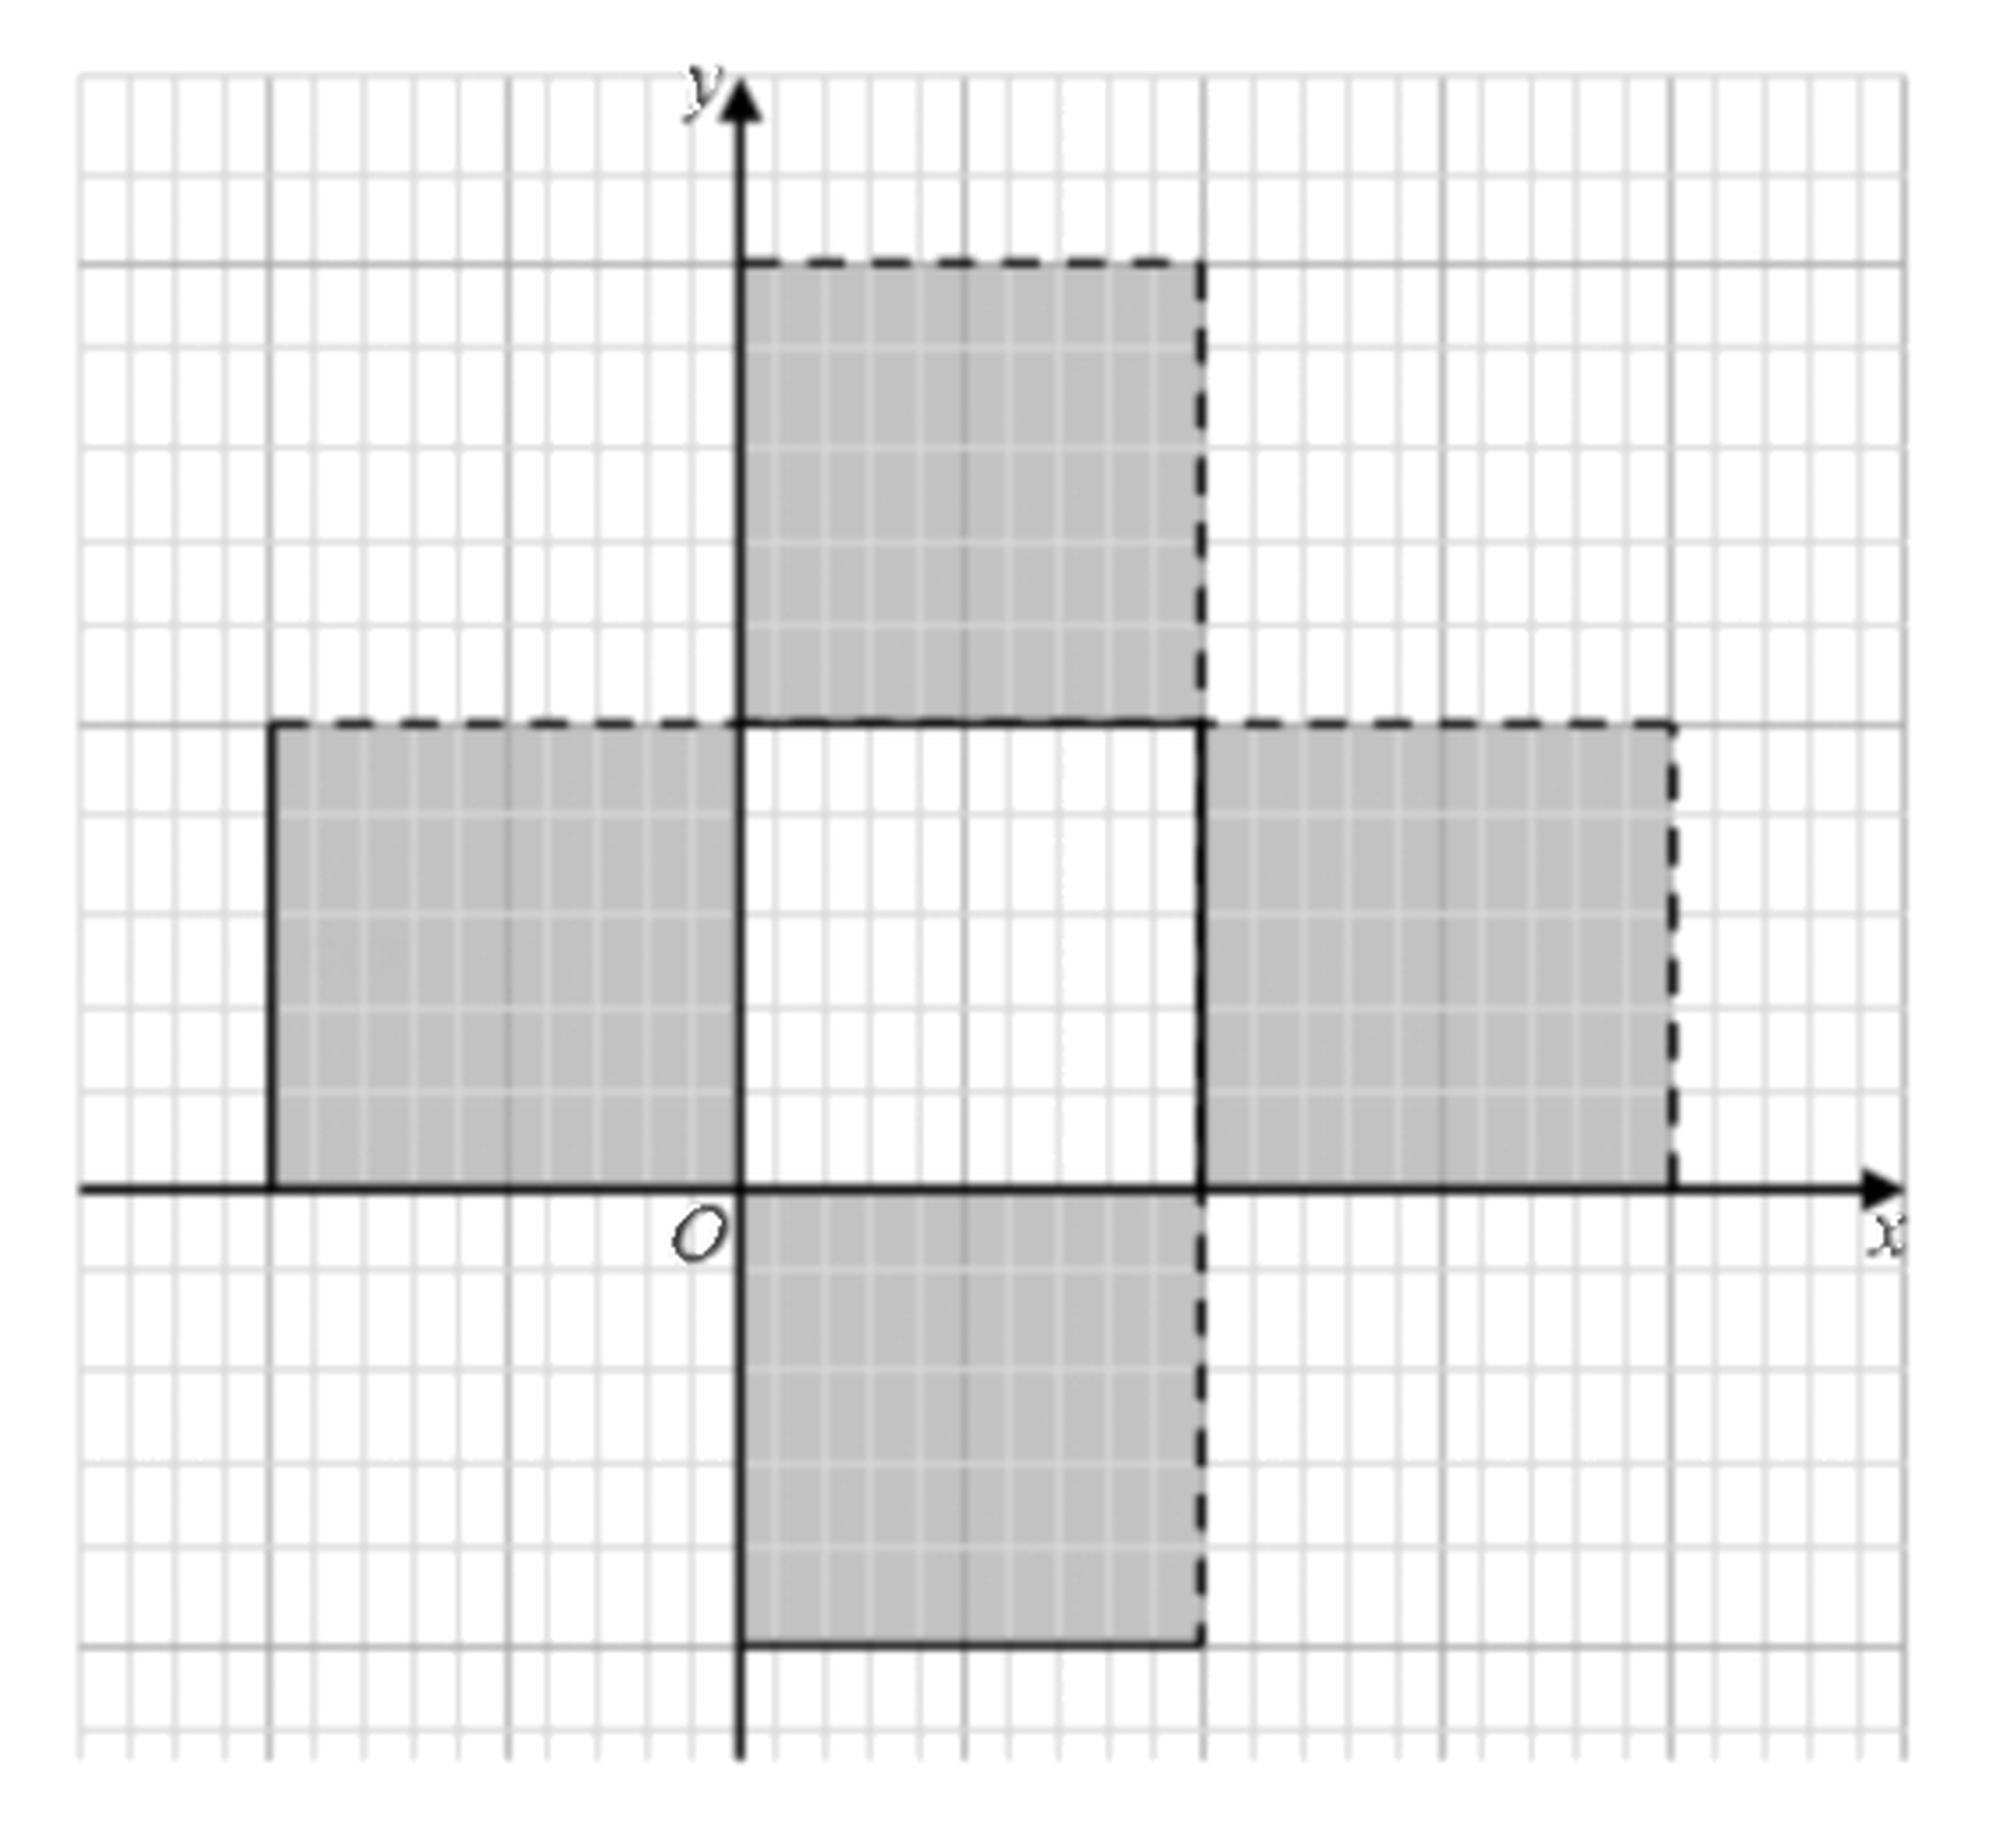
\includegraphics[width=0.34\textwidth]{figures/gao150_q12.png}
\end{center}
\step{总面积为 $1\times4=4$.}
\solend
\fi

\end{enumerate}

\bigsec{二、选择题}

\begin{enumerate}
\setcounter{enumi}{12}

% === Q13 === 答案在解析末句"故选 C"；括号 \mbox{（\quad）} 留空；四选项一行；解析 1 行
\item 设 $x\ne0$，则 $3^{\log_9 x^2}$ 的化简结果是\mbox{（\quad）}

\keepwithprev
A. $x$\qquad B. $\dfrac{1}{x}$\qquad C. $\lvert x\rvert$\qquad D. $\dfrac{1}{\lvert x\rvert}$

\ifanswer
\solbegin
\step{$3^{\log_9 x^2}=3^{\log_3\lvert x\rvert}=\lvert x\rvert$，故选 $C$.}
\solend
\fi

% === Q14 === 题目配图（两函数图像，三版都出）；\needvspace{8cm} 守卫放 \item 之前；"图像"照录；四选项两行两列；解析 2 行，故选 B
\needvspace{8cm}
\item 设 $a>0$ 且 $a\ne1$，$b\in\R$. 若函数 $y=a^{-\lvert x\rvert}$ 与 $y=x^b$ 的大致图像如图所示，则\mbox{（\quad）}

\keepwithprev
A. $0<a<1<b$\qquad\qquad B. $a>1$ 且 $b>1$

C. $0<a<1$ 且 $0<b<1$\qquad\qquad D. $0<b<1<a$

\begin{center}
% 两函数 y=a^{-|x|} 与 y=x^b 大致图像取 04 页右侧，去粉色水印、去色、4× LANCZOS 放大；三版都出
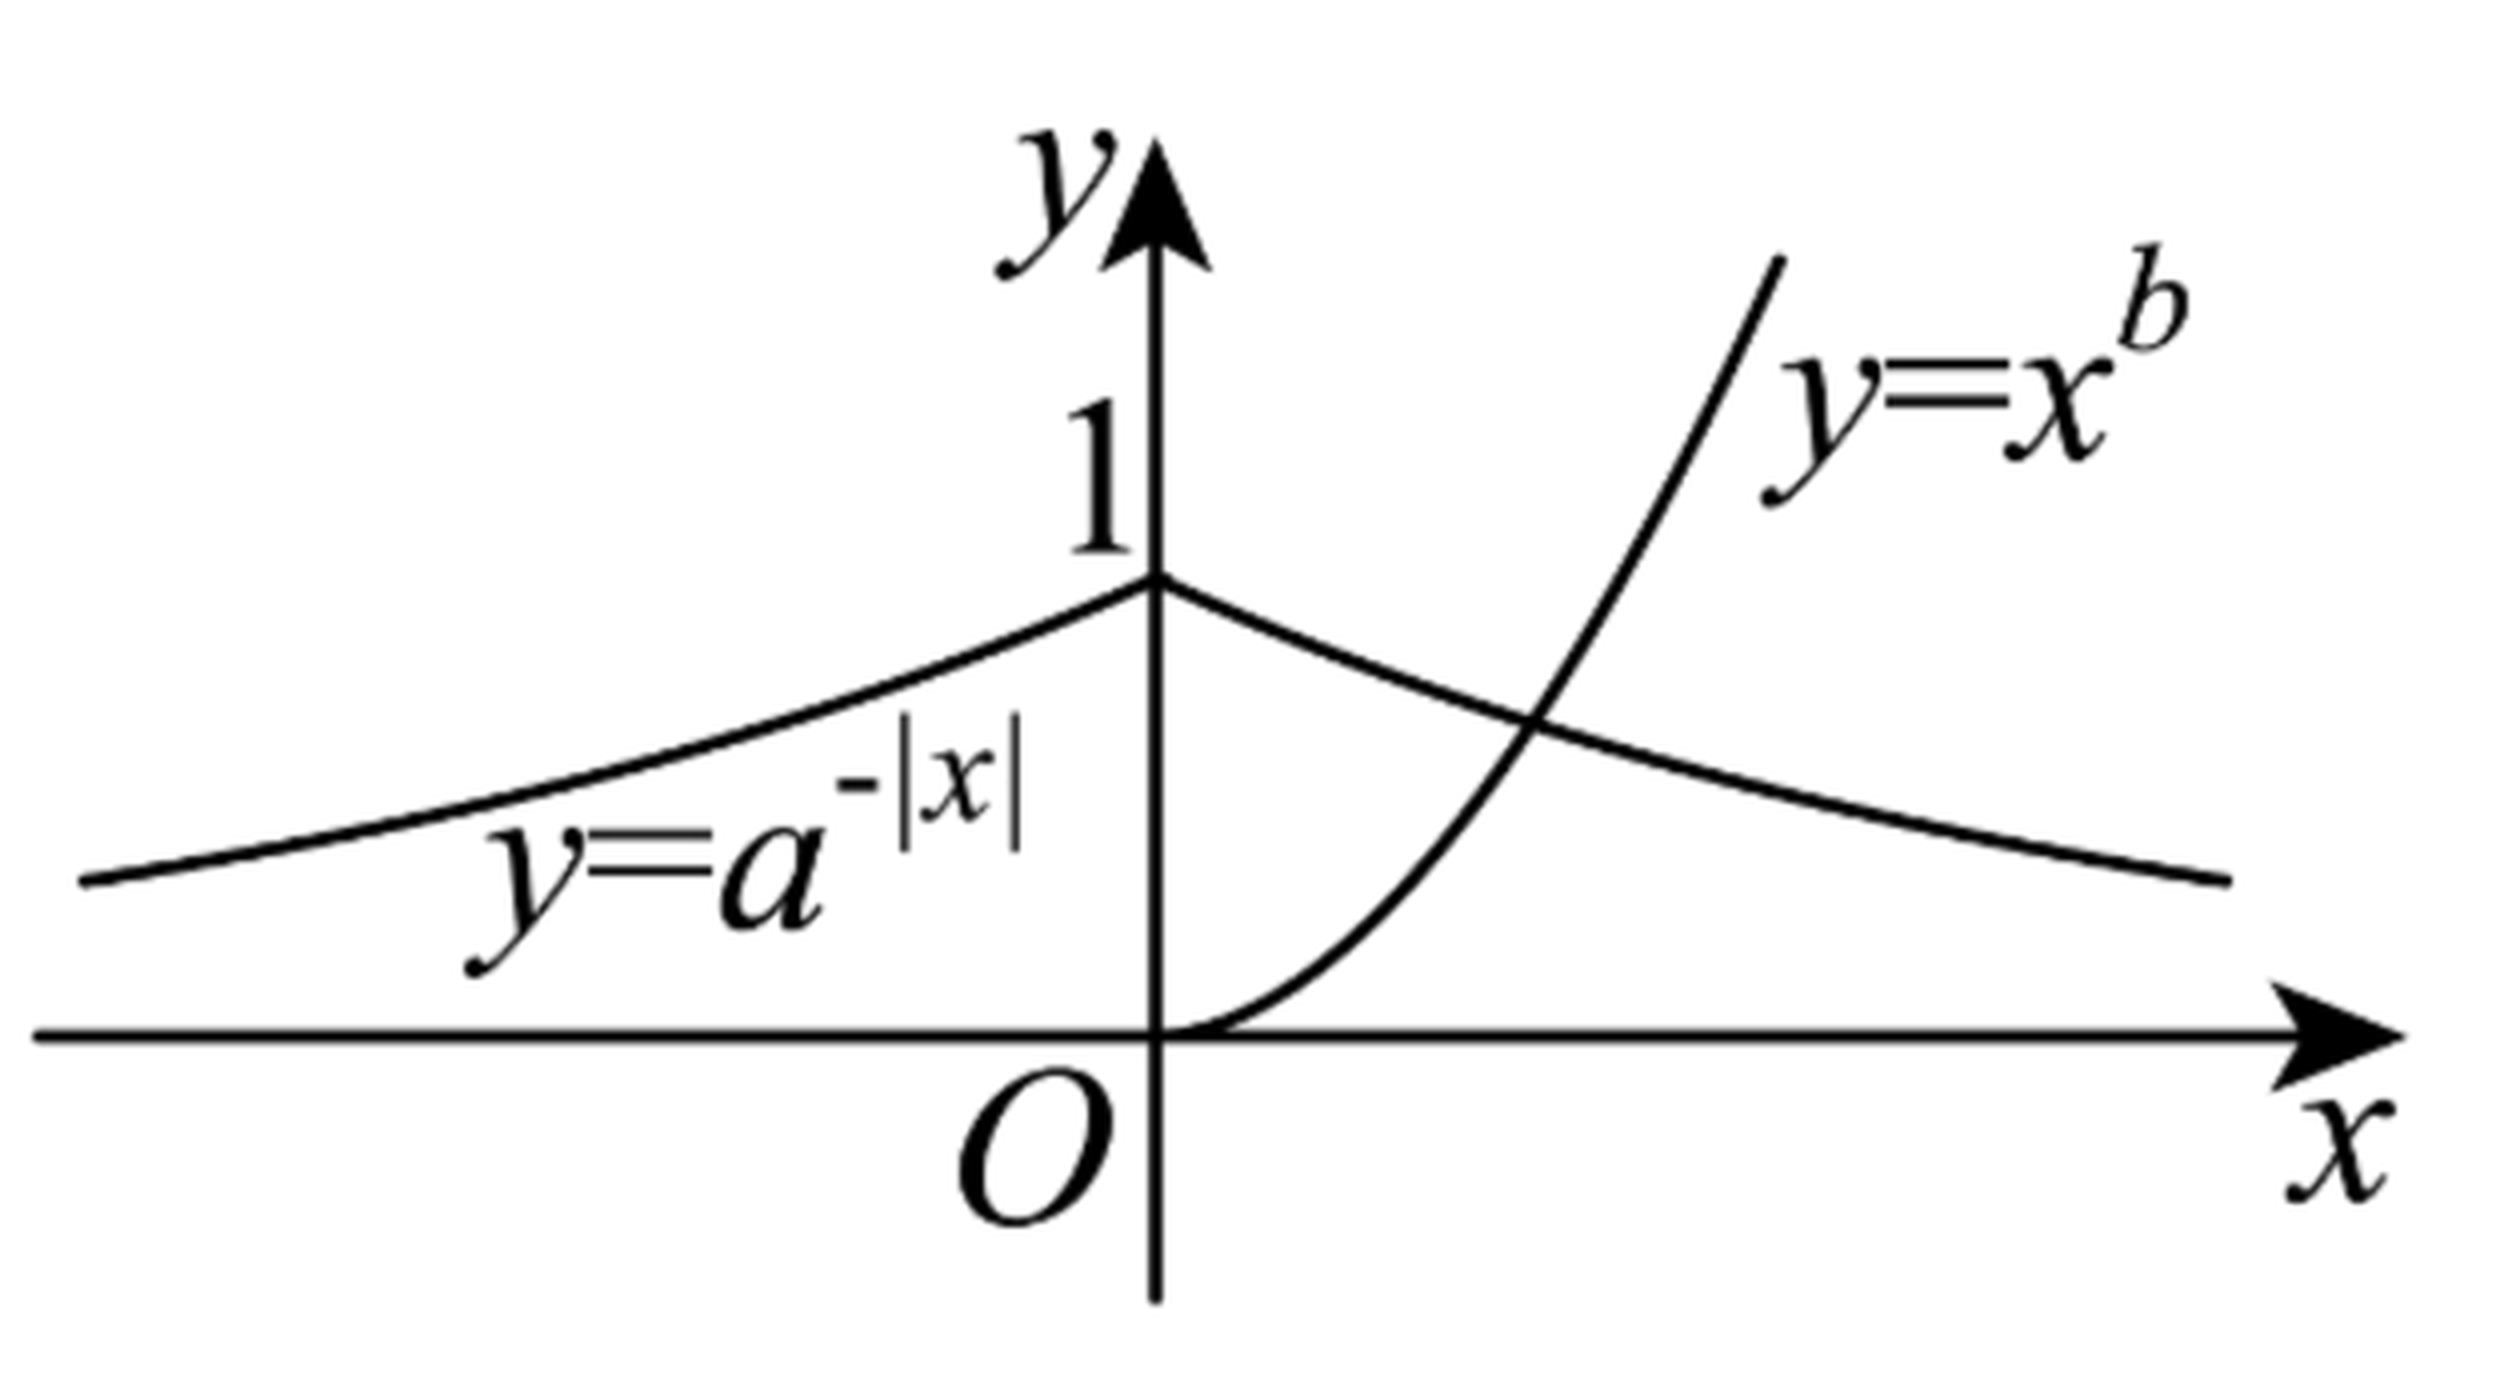
\includegraphics[width=0.40\textwidth]{figures/gao150_q14.png}
\end{center}

\ifanswer
\solbegin
\step{在 $(0,+\infty)$ 上，$y=a^{-x}$ 严格递减，得 $a>1$；}
\step{幂函数 $y=x^b$ 的图像递增且向上弯曲，得 $b>1$；故选 $B$.}
\solend
\fi

% === Q15 === "算术平均值／算术平均数"两处不同照录；四选项两行两列；解析 5 行（续 05 页顶），故选 B
\item 已知两个正数的算术平均值不小于它们的几何平均值，类比有以下结论：三个正数的算术平均数不小于它们的几何平均数，即当 $a,b,c$ 为正实数时，$\dfrac{a+b+c}{3}\geqslant\sqrt[3]{abc}$，当且仅当 $a=b=c$ 时等号成立. 利用上述结论，下列选项中判断正确的是\mbox{（\quad）}

\keepwithprev
A. 若 $x>0$，则 $2x+\dfrac{1}{x^2}\geqslant\dfrac{27}{8}$\qquad\qquad B. 若 $x>0$，则 $x^2+\dfrac{2}{x}\geqslant3$

C. 若 $0<x<1$，则 $x^2(1-x)\geqslant\dfrac{1}{9}$\qquad\qquad D. 若 $0<x<1$，则 $x^2(1-x)\leqslant\dfrac{1}{9}$

\ifanswer
\solbegin
\step{A：取 $x=1$，$2x+\dfrac{1}{x^2}=3<\dfrac{27}{8}$，错误.}
\step{B：$x^2+\dfrac{2}{x}=x^2+\dfrac{1}{x}+\dfrac{1}{x}\geqslant3\sqrt[3]{x^2\cdot\dfrac{1}{x}\cdot\dfrac{1}{x}}=3$，当且仅当 $x=1$ 时取等号，正确.}
\step{C：取 $x=\dfrac{1}{3}$，$x^2(1-x)=\dfrac{2}{27}<\dfrac{1}{9}$，错误.}
\step{D：取 $x=\dfrac{2}{3}$，$x^2(1-x)=\dfrac{4}{27}>\dfrac{1}{9}$，错误.}
\step{故选 $B$.}
\solend
\fi

% === Q16 === "完美集"新定义（弯引号、引号外空格照录）；圈数字①②文本模式；$n\in\N$；四选项两行两列；解析 9 行（6 行 05 页＋3 行 06 页顶），故选 A
\item 已知有限集 $A=\{a_1,a_2,\cdots,a_n\}$（$n\geqslant2$，$n\in\N$）. 若 $A$ 中元素 $a_i$（$i=1,2,\cdots,n$）满足 $a_1+a_2+\cdots+a_n=a_1\cdot a_2\cdots a_n$，就称 $A$ 为 “完美集”. 现有以下两个命题：

①恰有两个元素的 “完美集” 有无穷多个；

②若 $a_i$ 均为正整数，则 “完美集” $A$ 有且只有一个，且 $n=3$.

则\mbox{（\quad）}

\keepwithprev
A. ①和②都是真命题\qquad\qquad B. ①和②都是假命题

C. ①是真命题，②是假命题\qquad\qquad D. ①是假命题，②是真命题

\ifanswer
\solbegin
\step{①由 $a+b=ab\Leftrightarrow(a-1)(b-1)=1$，任取 $a>2$，则 $b=1+\dfrac{1}{a-1}\in(1,2)$，}
\step{得到无穷多个不同的完美集，①真.}
\step{②设 $1\leqslant a_1<a_2<\cdots<a_n$，则 $a_i\geqslant i$.}
\step{若 $n=2$，则 $(a_1-1)(a_2-1)=1$，只能有 $a_1=a_2=2$，与元素互异矛盾.}
\step{若 $n\geqslant4$，则 $a_1a_2\cdots a_n\geqslant a_2a_{n-1}a_n\geqslant2(n-1)a_n>na_n\geqslant a_1+\cdots+a_n$，矛盾.}
\step{当 $n=3$ 时，若 $a_1\geqslant2$，则 $a_1a_2a_3\geqslant6a_3>3a_3\geqslant a_1+a_2+a_3$，矛盾.}
\step{因此 $a_1=1$，$(a_2-1)(a_3-1)=2$，结合 $a_2<a_3$ 得 $a_2=2$，$a_3=3$.}
\step{唯一的完美集为 $\{1,2,3\}$，②真.}
\step{故选 $A$.}
\solend
\fi

\end{enumerate}

\bigsec{三、解答题}

\begin{enumerate}
\setcounter{enumi}{16}

% === Q17 === \varnothing 空集、$B\subseteq A$ 带下划线照录；弯引号内空格照录；解析 7 行
\item 设 $a,b\in\R$. 已知集合 $A=\{x\mid ax^2+3x-a>3\}$，$B=\{x\mid bx=1\}$.

(1) 若 $A=(1,2)$，求 $a$ 的值；

(2) 若 $a=0$，且 “ $x\in A$ ” 是 “ $x\in B$ ” 的必要非充分条件，求 $b$ 的取值范围.

\ifanswer
\solbegin
\step{(1) $A=(1,2)$，则 $a<0$，且 $1,2$ 是方程 $ax^2+3x-a-3=0$ 的两根.}
\step{由 $4a+6-a-3=0$，得 $a=-1$，此时不等式为 $-(x-1)(x-2)>0$，}
\step{解集确为 $(1,2)$.}
\step{(2) $a=0$ 时，$A=(1,+\infty)$，题意等价于 $B\subseteq A$ 且 $B\ne A$.}
\step{当 $b=0$ 时，$B=\varnothing$，符合条件.}
\step{当 $b\ne0$ 时，$B=\left\{\dfrac{1}{b}\right\}$，条件等价于 $\dfrac{1}{b}>1$，解得 $0<b<1$.}
\step{因此 $b$ 的取值范围为 $[0,1)$.}
\solend
\fi

% === Q18 === $p\in\Z$；"图像"（像，有亻）照录；指数 $-2p^2+5p$；解析 8 行（(1) 首行 06 页末＋2 行 07 页顶、(2) 5 行 07 页）
\item 设 $p\in\Z$，已知 $f(x)=x^{-2p^2+5p}$.

(1) 若幂函数 $y=f(x)$ 的图像关于原点成中心对称，且满足 $f(3)<f(4)$，求 $p$ 的值；

(2) 当 $p=-2$ 时，求满足 $f(2x+3)<f(x-4)$ 的 $x$ 的取值范围.

\ifanswer
\solbegin
\step{(1) 图像关于原点成中心对称，得整数 $-2p^2+5p$ 为奇数.}
\step{由 $f(3)<f(4)$，得 $-2p^2+5p>0\Leftrightarrow0<p<\dfrac{5}{2}$，}
\step{结合 $p\in\Z$，得 $p=1$ 或 $p=2$，对应指数分别为 $3$、$2$，所以 $p=1$.}
\step{(2) 当 $p=-2$ 时，$f(x)=\dfrac{1}{x^{18}}$，定义域为 $\{x\in\R\mid x\ne0\}$.}
\step{原不等式要求 $x\ne-\dfrac{3}{2}$ 且 $x\ne4$，}
\step{此时 $\dfrac{1}{(2x+3)^{18}}<\dfrac{1}{(x-4)^{18}}\Leftrightarrow\lvert 2x+3\rvert>\lvert x-4\rvert\Leftrightarrow(2x+3)^2>(x-4)^2$，}
\step{因此 $(x+7)(3x-1)>0\Leftrightarrow x<-7$ 或 $x>\dfrac{1}{3}$，}
\step{排除 $x=4$，得 $x\in(-\infty,-7)\cup\left(\dfrac{1}{3},4\right)\cup(4,+\infty)$.}
\solend
\fi

% === Q19 === $a\in\R$、$g(x)=f(2x+1)+a\cdot f(x)+2$；解析 6 行（(2) 末两行续 08 页顶）
\item 已知 $f(x)=2^x$.

(1) 求方程 $f(2x)-f(x)=6$ 的解；

(2) 设 $a\in\R$，$g(x)=f(2x+1)+a\cdot f(x)+2$，若对于任意 $x\in[-1,1]$，均有 $g(x)\geqslant1$，求 $a$ 的取值范围.

\ifanswer
\solbegin
\step{(1) 令 $t=2^x>0$，则 $t^2-t-6=(t-3)(t+2)=0$，}
\step{由 $t>0$ 得 $t=3$，所以 $x=\log_2 3$.}
\step{(2) 令 $t=2^x$，则 $t\in\left[\dfrac{1}{2},2\right]$，且 $g(x)\geqslant1\Leftrightarrow2t^2+at+1\geqslant0\Leftrightarrow a\geqslant-\left(2t+\dfrac{1}{t}\right)$，}
\step{由基本不等式得 $2t+\dfrac{1}{t}\geqslant2\sqrt{2t\cdot\dfrac{1}{t}}=2\sqrt2$，}
\step{当且仅当 $t=\dfrac{1}{\sqrt2}\in\left[\dfrac{1}{2},2\right]$ 时等号成立，}
\step{因此 $-\left(2t+\dfrac{1}{t}\right)$ 的最大值为 $-2\sqrt2$，所求范围为 $a\in[-2\sqrt2,+\infty)$.}
\solend
\fi

% === Q20 === "极闭集"新定义、3 问，全卷末题；$M\subseteq(0,+\infty)$ 带下划线照录；自定义运算 $x*y$ 星号照录；解析 13 行（9 行 08 页＋4 行 09 页上半）
\item 对于非空实数集 $M\subseteq(0,+\infty)$，若满足以下两个条件：

① $M$ 中至少含有 $2$ 个元素，且 $1\notin M$；

②对于 $M$ 中任意两个不相等的元素 $x$、$y$，定义 $x*y=\dfrac{xy+1}{x+y}$，且 $x*y\in M$.

则称 $M$ 为 “极闭集”.

(1) 分别判断集合 $A=\left\{\dfrac{1}{2},3\right\}$ 与集合 $B=(1,+\infty)$ 是否为 “极闭集” （无需理由）；

(2) 若 $M$ 是 “极闭集”，证明：$M$ 中不可能所有元素都小于 $1$；

(3) 证明：不存在任何有限集是 “极闭集”.

\ifanswer
\solbegin
\step{(1) $A$ 不是 “极闭集”，$B$ 是 “极闭集”.}
\step{(2) 假设 $M$ 中所有元素都小于 $1$，取其中两个不相等的元素 $x$、$y$，}
\step{则 $x*y-1=\dfrac{(1-x)(1-y)}{x+y}>0$，}
\step{这与 $x*y\in M$ 且 $M$ 中所有元素都小于 $1$ 矛盾.}
\step{(3) 假设有限集 $M$ 是 “极闭集”，}
\step{由 (2) 及 $1\notin M$，得 $M$ 中存在大于 $1$ 的元素.}
\step{若 $M$ 中有小于 $1$ 的元素，取其中最大的一个为 $a$，另取 $b\in M$ 且 $b>1$，}
\step{则 $a*b-a=\dfrac{1-a^2}{a+b}>0, a*b-1=\dfrac{(a-1)(b-1)}{a+b}<0$，}% 半角逗号在两个数学式组之间，全稿惯例、非笔误，照录
\step{于是 $a<a*b<1$ 且 $a*b\in M$，与 $a$ 的最大性矛盾.}
\step{若 $M$ 中没有小于 $1$ 的元素，则 $M\subseteq(1,+\infty)$.}
\step{取 $a=\min M$，另取 $b\in M$ 且 $b\ne a$，则 $a*b-a=\dfrac{1-a^2}{a+b}<0$，}
\step{于是 $a*b<a$ 且 $a*b\in M$，与 $a$ 的最小性矛盾.}
\step{因此不存在任何有限集是 “极闭集”.}
\solend
\fi

\end{enumerate}

\end{document}
"
%
% ① 原始材料：微信公众号"魔都数学加油站"文章，连载"27学年高一150"，原文标题
% "27学年高一150——2026-2027年上海市曹杨二中高一上期中"；
% 原文链接：https://mp.weixin.qq.com/s/xlQxmik8TZXR87RC6MnCrw 。
% 正文为 9 张 PNG 页（01/02/04/06/07/09 为 2560×3620，03/05/08 为 4762×6735，
% 同一篇各页分辨率混排，逐页按各自分辨率裁图核对，别按预览比例换算裁框）。
% 体例：讲评版——全 18 题均印【解析】（逐题核实，见 ② ②）。
% 题目、答案、解析均据原图转录；卷面粉红色/红色水印"魔都数学加油站"及公众号页脚未录入。
% 全卷插图清单（逐页通读 9 页确认）：3 幅——
%   · Q11 题目配图（指数函数曲线图，02 页右侧：x/y 轴、O、y=2^x 与 y=2^{x+1}
%     两曲线、A/B/C 三点、刻度 1/2、等边三角形 ABC），三版都出，裁 figures/gao150_q11.png；
%   · Q12 解析配图（高斯函数取整 [x]^2+[y]^2=1 方格阴影区域图，04 页顶部：4 个边长 1
%     的正方形组成的十字形阴影），解析"作出平面区域如图所示"处，仅答案版出，
%     放 \ifanswer 内 \step 之间，裁 figures/gao150_q12.png；
%   · Q14 题目配图（两函数 y=a^{-|x|} 与 y=x^b 大致图像，04 页右侧：x/y 轴、O、
%     y 轴刻度 1、一递减曲线一递增上翘曲线），三版都出，裁 figures/gao150_q14.png；
%   其余各页逐页确认无其它题目配图、无表格；Q11/Q12 解析"如图所示"对应的就是上列
%   已裁的图，不重复裁；09 页上半为 Q20(3) 解析续尾、下半仅水印、无正文。
%   3 图均取自原卷截图，去粉色水印、去色、4× LANCZOS 放大。
%
% 卷首标题：原卷印作"2026-2027 年曹杨二中高一上期中"，年份区间按全稿惯例排 en dash；
% 原卷卷面未印副标题，本稿按同期中卷知识模块口径补出"集合与常用逻辑用语、不等式、函数"。
%
% 题号体例（逐页核实定稿）：本卷共 18 题——一、填空题 3—12（10 题）、
% 二、选择题 13—16（4 题）、三、解答题 17—20（4 题）。
% 三节分别 \setcounter{enumi}{2}／{12}／{16}。原卷从第 3 题起、无第 1、2 题，
% 本稿保留原题号；全卷末题为第 20 题（"极闭集"新定义、3 问），无 Q21、无附加题节。
%
% ② 与原卷的排版差异：
%   ① 原文从第 3 题起，本稿保留原题号；共 18 题三节，解答题只有 4 题到 20；
%   ② 全 18 题均印【解析】，用 \solbegin…\solend；逐题核实无只印【答案】或
%      答案印题干括号内的题；四道选择题答案在解析末句"故选 X"（Q13 选 C、
%      Q14 选 B、Q15 选 B、Q16 选 A，逐个放大复核）、括号 \mbox{（\quad）} 留空、
%      不另提 \ans{}；答案版【答案】/【解析】标记数 = 18 = 全卷题数；
%   ③ 原卷卷面未印副标题，本稿按知识模块口径补出；
%   ④ 原卷填空横线按全稿惯例排 \blankline[4.4em]；选择题括号排 \mbox{（\quad）}、
%      选项段前按惯例加 \keepwithprev；解答题不留作答区、不加 \anspace（原卷为讲评版）；
%   ⑤ 数集黑板粗体：Q4"m\in R"、Q5"a,b\in R"、Q6"a,b,c\in R"、Q7"a\in R"、
%      Q10"a\in R"、Q14"b\in R"、Q17"a,b\in R"、Q18"p\in Z"／定义域"x\in R"、
%      Q19"a\in R"、Q16"n\in N" 原卷印斜体 R/Z/N，按全稿惯例归一 \R／\Z／\N；
%      绝对值排 \lvert…\rvert（Q7 |x+4|+|x-3|、Q11 |AB|／|CD|、Q13 |x|、
%      Q18 |2x+3|／|x-4|），集合描述竖线排 \mid（Q3、Q12、Q17、Q18、Q20），
%      不等号按全稿惯例排 \leqslant／\geqslant；补集照原卷上划线排 \overline{A}
%      （Q3 题干＋解析共 2 处）；空集符号 \varnothing（Q17 解析(2)）；
%      子集 \subset（单线⊂）／\subseteq（带下划线⊆）逐处照录，本卷 3 处子集
%      符号均印带下划线 ⊆、照录 \subseteq（Q20 题干、Q20 解析(3)、Q17 解析(2)，
%      见 ④），无 \subset 用例；
%   ⑥ 判别式 Δ/△：逐页通读 9 页，本卷无一元二次判别式算式，故无 Δ/△ 混用可照录
%      （"高 \Delta／扁 \triangle"口径备查，参照 高一142／144／145／146／148／149
%      头注④）；本卷仅 Q11 题干与解析共 2 处几何三角形符号 △ABC，逐处放大并排
%      确认两处同形、印近等边粗线三角（非判别式），照录 \triangle（见 ④）；
%   ⑦ 中文弯引号照录：Q12"数学王子"、Q16"完美集"（题干＋①②两命题，引号外
%      留空格）、Q17" x∈A "" x∈B "（引号内空格）、Q20"极闭集"（题干条件、
%      三问与解析，引号外留空格）；注释里一律 ASCII 引号；数学式内 CJK 用 \text{}
%      （Q3 集合描述"且"用 \text{ 且 }）；
%   ⑧ 半角逗号在数学组之间是全稿惯例、非笔误，逐处照录（Q17 解析"1,2 是方程…
%      两根"、Q20 解析(3)">0, a*b-1=…<0" 两式之间等）；行末西文句点 ASCII `.`；
%      行中全角逗号／顿号照录（Q12"之一、享有"、Q18 解析"3、2"、Q20"x、y"）；
%   ⑨ "图像／图象"逐处放大核：全卷 9 处均印"图像"（像，有亻）、未见"图象"——
%      Q4 题干 1、Q11 题干 2＋解析 1、Q14 题干 1＋解析 1、Q18 题干 1＋解析 1；
%      同卷"第二象限""象限"用"象"（无亻）。逐处照录未统一改动（放大 01/02/04/06
%      页 /tmp/gao150/z/p01_q4_tuxiang2.png、p04_q14_tuxiang2.png、
%      p02_q11_lines.png 确认）；子题标号 (1)(2)(3) 半角括号照录；圈数字①②
%      在文本模式（Q16 两命题与解析、Q20 两条件与三问及解析）按 common.sty
%      划入 CJK 字符类渲染，进数学式用 \text{①}；
%   ⑩ Q20 新定义 x*y=\dfrac{xy+1}{x+y} 的 * 是自定义运算（星号），照录；
%      \left…\right 不得拆到不同 $…$ 组（Q19"\left(2t+\frac1t\right)"、
%      Q20 题干"A=\left\{\frac12,3\right\}"等）；Q8 嵌套根号
%      \sqrt{\frac2x+\frac{16}{1-2x}}、Q9 对数连加 \log_2 A 等复杂式照录别简化；
%   ⑪ 一条 \step = 原卷解析的一个印刷行，cases 块整体算一个印刷行；别并折行、
%      别拆行。Q4 三行、Q8 五行、Q11 九行、Q12 四行（两行各含四个 cases 块）、
%      Q15 五行、Q16 九行、Q18 八行、Q20 十三行均按印刷行逐条断，不丢行；
%   ⑫ 配图：Q11／Q14 题目配图（三版都出）放 \item 内题干之后 \begin{center}，
%      大图块加 \needvspace{8cm} 守卫把整块推走（守卫放 \item 之前，见
%      高一145 Q14/Q20 成例与切页审计 B 类坑）；Q12 解析配图（仅答案版出）
%      放 \ifanswer 内 \solbegin…\solend 的 \step 之间（高一73 第16题成例）；
%   ⑬ 跨页续印按题合并：见 ⑥；
%   ⑭ 原卷解析内无红色"法一／法二"之类小标题，故本卷无 \stepm；红色水印
%      "魔都数学加油站"不录入；Q12 解析"作出平面区域如图所示"对应的图即
%      ① 所列 gao150_q12.png（04 页顶部），不重复裁；Q11 解析"如图所示"对应
%      题目配图 gao150_q11.png，不另裁。
%
% ③ 行数复核：一条 \step／\stepm = 原卷解析的一个印刷行，cases 块作一个印刷行计。
%   逐题数（主会话逐页核对定稿）：Q3：1；Q4：3；Q5：2；Q6：1；Q7：2；Q8：5；
%   Q9：1；Q10：3；Q11：9；Q12：4；Q13：1；Q14：2；Q15：5；Q16：9；
%   Q17：7；Q18：8；Q19：6；Q20：13。
%   合计 82 条 \step（本卷无 \stepm：解析内无红色"法一／法二"类小标题），
%   与原卷逐题印刷行相等。全卷 18 题均设 \solbegin…\solend，答案版
%   【答案】/【解析】标记数 = 18 = 全卷题数。
%
% ④ 判别式／三角形／子集符号结论（逐处放大原图照录、不得统一，主会话像素级复核）：
%   判别式：逐页通读 9 页，本卷无一元二次判别式 Δ/△ 算式（Q18 讨论幂函数指数
%     奇偶、不用判别式；Q9／Q19／Q20 亦无），头注 ② ⑥ 的"高 \Delta／扁 \triangle"
%     口径在本卷无对应处（参照 高一142／144／145／146／148／149 头注④，仅备查）。
%   几何三角形符号：Q11 题干"使得 △ABC 为等边三角形"（02 页末）与解析
%     "因为 △ABC 为等边三角形，则 CD⊥AB"（03 页）共 2 处，放大 02/03 页
%     /tmp/gao150/z/q11_tri_montage2.png 并排确认两处同形、印近等边粗线三角
%     （h/w≈0.98、非"高>宽"的判别式 \Delta），照录 \triangle（与 高一105
%     "使得 \triangle ABC 为等边三角形" 同短语成例、高一149 几何三角形照录
%     \triangle 口径一致），不引入 \Delta。
%   子集／补集：Q20 题干"$M\subseteq(0,+\infty)$"（08 页）、Q20 解析(3)
%     "则 $M\subseteq(1,+\infty)$"（09 页）、Q17 解析(2)"题意等价于 $B\subseteq A$
%     且 $B\ne A$"（06 页）共 3 处子集符号，逐处放大（/tmp/gao150/z/p08_q20_stem.png、
%     p09_q20_sub.png、p06_q17_sub.png）确认均印带下划线 ⊆，照录 \subseteq；
%     本卷未见单线 ⊂（\subset）之对应处。Q3 题干与解析共 2 处补集照原卷上划线
%     排 \overline{A}；Q17 解析(2) 空集印 ∅、照录 \varnothing（Q7"解集为空集"
%     为中文词、非符号，照录文字）；集合描述竖线 \mid；数集 \R／\Z／\N 归一见 ② ⑤。
%
% ⑤ 存疑照录（放大原图确认，照录未改、正文对应处另有 % 注）：
%   1. Q8 解析第 4 行"所以 $y=\frac1x+\frac{8}{1-2x}$ 的最小值为 18" —— 上文
%      并未定义 $y$，且题面求的是 $\sqrt{\frac2x+\frac{16}{1-2x}}$ 的最小值；
%      按上下文该行应为 $\frac1x+\frac{8}{1-2x}$ 的最小值为 18（$y$ 疑为原卷
%      衍字／笔误），放大 02 页 /tmp/gao150/z/p02_q8_y.png 确认，照录未改。
%   2. Q20 解析(3)"$a*b-a=\frac{1-a^2}{a+b}>0, a*b-1=\frac{(a-1)(b-1)}{a+b}<0$"
%      两式之间的逗号原卷印半角 ,（非全角），按全稿惯例"半角逗号在数学组之间"
%      照录未改（放大 08 页 /tmp/gao150/z/p08_q20_sol8.png 确认）。
%   3. Q15 题干"两个正数的算术平均值…几何平均值"与"三个正数的算术平均数…
%      几何平均数"两处"值／数"用字不同，逐处照录未统一（放大 04 页确认）。
%   4. "图像／图象"全卷 9 处均印"图像"（像，有亻）、未见"图象"，逐处放大核实
%      照录、未统一改动（见 ② ⑨）；本卷判别式 Δ/△ 无用例、几何三角形 2 处
%      照录 \triangle（见 ④）。
%   全卷除此 4 类外未发现其它笔误／自相矛盾处；18 题均印【解析】、无只印【答案】
%   或答案印题干括号内的题（见 ② ②）。
%
% ⑥ 跨页续印按题合并说明（逐页核实定稿）：Q3/4/5/6/7 题干＋解析在 01 页；
%   Q8 题干＋解析 5 行、Q9 题干＋解析 1 行在 02 页上半；Q10 题干＋解析 3 行
%   在 02 页下半；Q11 题干（前两行）＋配图在 02 页下半、题干续"三角形，则点 C
%   的纵坐标为___"与解析 9 行全在 03 页上半（解析"如图所示"对应题目配图）；
%   Q12 题干＋解析 4 行在 03 页下半，解析配图（方格阴影）续印在 04 页顶部；
%   "二、选择题"标题在 04 页中部；Q13 题干＋选项＋解析、Q14 题干＋选项＋
%   配图＋解析在 04 页；Q15 题干＋四选项在 04 页末、解析 5 行续 05 页上半；
%   Q16 题干＋①②两命题＋"则(  )"＋四选项＋解析前 6 行在 05 页、解析末 3 行
%   （"因此 a_1=1…②真""故选 A"）续 06 页顶部；"三、解答题"标题在 06 页；
%   Q17 题干(1)(2)＋解析(1) 3 行＋解析(2) 首行在 06 页、解析(2) 续 3 行
%   在 06 页下半；Q18 题干(1)(2)＋解析(1) 首行在 06 页末、解析(1) 续 2 行＋
%   解析(2) 5 行在 07 页上半；Q19 题干(1)(2)＋解析(1) 2 行＋解析(2) 前 2 行
%   在 07 页下半、解析(2) 末 2 行续 08 页顶部；Q20 题干（新定义＋①②两条件）
%   ＋三问＋解析(1)(2)(3) 前 9 行在 08 页、解析(3) 末 4 行续 09 页上半，
%   末行"因此不存在任何有限集是极闭集"为全卷收尾（09 页下半仅水印、无正文）。
%   本稿按题连排，不丢行、不并折行；全卷末题为第 20 题，无 Q21、无附加题节。
%
\documentclass[a4paper,11pt]{article}
\usepackage{common}

\begin{document}

\examtitlest[3]{2026--2027 年曹杨二中高一上期中}{集合与常用逻辑用语、不等式、函数}

\bigsec{一、填空题}

\begin{enumerate}
\setcounter{enumi}{2}

% === Q3 === 补集上划线 \overline{A}（题干＋解析各 1 处）；集合描述竖线 \mid、数学式内"且"用 \text{}；解析 1 行
\item 设全集 $U=\{1,2,3,4,5\}$，集合 $A=\{x\mid x^2-3x\leqslant0\text{ 且 }x\in U\}$，则 $\overline{A}=$\blankline[4.4em].

\ifanswer
\solbegin
\step{$x^2-3x\leqslant0\Leftrightarrow0\leqslant x\leqslant3$，所以 $A=\{1,2,3\}$，$\overline{A}=\{4,5\}$.}
\solend
\fi

% === Q4 === "图像"（像，有亻）逐处照录、同句"第二象限"用"象"（无亻）；解析 3 行
\item 设 $m\in\R$. 若幂函数 $y=(m^2-5m+1)x^{m+1}$ 的图像经过第二象限，则 $m=$\blankline[4.4em].

\ifanswer
\solbegin
\step{幂函数的系数为 1，故 $m^2-5m+1=1\Rightarrow m=0$ 或 $m=5$.}
\step{$m=0$ 时，$y=x$ 不经过第二象限；}
\step{$m=5$ 时，$y=x^6$ 经过第二象限，因此 $m=5$.}
\solend
\fi

% === Q5 === 解析 2 行
\item 设 $a,b\in\R$. 若 $a^2+\dfrac{b^2}{4}=1$，则 $ab$ 的最大值为\blankline[4.4em].

\ifanswer
\solbegin
\step{$1-ab=\left(a-\dfrac{b}{2}\right)^2\geqslant0$，即 $ab\leqslant1$；}
\step{当 $a=\dfrac{\sqrt2}{2}$，$b=\sqrt2$ 时取等号，最大值为 1.}
\solend
\fi

% === Q6 === 解析 1 行
\item 设 $a,b,c\in\R$. 若等式 $2x^2-3x-2=a(x-1)^2+b(x-1)+c$ 恒成立，则 $a-b+c=$\blankline[4.4em].

\ifanswer
\solbegin
\step{令 $x=0$，得 $a-b+c=-2$.}
\solend
\fi

% === Q7 === 绝对值 \lvert…\rvert；解析 2 行
\item 设 $a\in\R$. 若关于 $x$ 的不等式 $\lvert x+4\rvert+\lvert x-3\rvert<a$ 的解集为空集，则 $a$ 的取值范围是\blankline[4.4em].

\ifanswer
\solbegin
\step{$\lvert x+4\rvert+\lvert x-3\rvert\geqslant\lvert(x+4)-(x-3)\rvert=7$，当 $-4\leqslant x\leqslant3$ 时取等号.}
\step{原不等式的解集为空集当且仅当 $a\leqslant7$，即 $a\in(-\infty,7]$.}
\solend
\fi

% === Q8 === 嵌套根号 \sqrt{\frac{2}{x}+\frac{16}{1-2x}} 照录别简化；解析 5 行
\item 设 $x\in\left(0,\dfrac{1}{2}\right)$，则 $\sqrt{\dfrac{2}{x}+\dfrac{16}{1-2x}}$ 的最小值为\blankline[4.4em].

\ifanswer
\solbegin
\step{因为 $x\in\left(0,\dfrac{1}{2}\right)$，所以 $1-2x>0$，又 $2x+1-2x=1$，}
\step{所以 $\left(\dfrac{1}{x}+\dfrac{8}{1-2x}\right)(2x+1-2x)=10+\dfrac{1-2x}{x}+\dfrac{16x}{1-2x}$}
\step{$\geqslant10+2\sqrt{\dfrac{1-2x}{x}\cdot\dfrac{16x}{1-2x}}=18$，}
\step{当且仅当 $\dfrac{1-2x}{x}=\dfrac{16x}{1-2x}$ 即 $x=\dfrac{1}{6}$ 时取等号，所以 $y=\dfrac{1}{x}+\dfrac{8}{1-2x}$ 的最小值为 18，}% 原卷此处径写 $y=\frac1x+\frac{8}{1-2x}$（上文未定义 $y$、且与题面根式不符），疑笔误，放大 02 页确认，照录未改（见 ⑤）
\step{所以 $\sqrt{\dfrac{2}{x}+\dfrac{16}{1-2x}}$ 的最小值为 6.}
\solend
\fi

% === Q9 === 对数连加 \log_2 A 等复杂式照录别简化；解析 1 行
\item 记 $A=1\times2\times3\times\cdots\times2026$，则 $\dfrac{1}{\log_2 A}+\dfrac{1}{\log_3 A}+\dfrac{1}{\log_4 A}+\cdots+\dfrac{1}{\log_{2026}A}=$\blankline[4.4em].

\ifanswer
\solbegin
\step{原式 $=\log_A 2+\cdots+\log_A 2026=\log_A(2\times3\times\cdots\times2026)=\log_A A=1$.}
\solend
\fi

% === Q10 === "严格减函数／不恒为负／⇔"照录；解析 3 行
\item 设 $a\in\R$，$f(x)=\dfrac{ax+1}{x+2}$. 若函数 $y=f(x)$ 在 $[1,+\infty)$ 上是严格减函数，且在 $[1,+\infty)$ 上的函数值不恒为负，则 $a$ 的取值范围是\blankline[4.4em].

\ifanswer
\solbegin
\step{当 $1\leqslant x_1<x_2$ 时，$f(x_2)-f(x_1)=\dfrac{(2a-1)(x_2-x_1)}{(x_1+2)(x_2+2)}$，故严格递减 $\Leftrightarrow a<\dfrac{1}{2}$.}
\step{此时最大函数值为 $f(1)$，函数值不恒为负 $\Leftrightarrow f(1)=\dfrac{a+1}{3}\geqslant0\Leftrightarrow a\geqslant-1$，}
\step{得 $a\in\left[-1,\dfrac{1}{2}\right)$.}
\solend
\fi

% === Q11 === 题目配图（指数函数曲线，三版都出）；\needvspace{8cm} 守卫放 \item 之前；"图像"照录、几何三角形 \triangle；解析 9 行（全在 03 页）
\needvspace{8cm}
\item 如图，点 $C$ 是函数 $y=2^x$ 的图像上的一点，若存在平行于 $x$ 轴的直线 $l$ 分别与函数 $y=2^x$ 和 $y=2^{x+1}$ 的图像相交于点 $A$、$B$，使得 $\triangle ABC$ 为等边三角形，则点 $C$ 的纵坐标为\blankline[4.4em].

\begin{center}
% 指数函数曲线图取 02 页右侧，去粉色水印、去色、4× LANCZOS 放大；三版都出
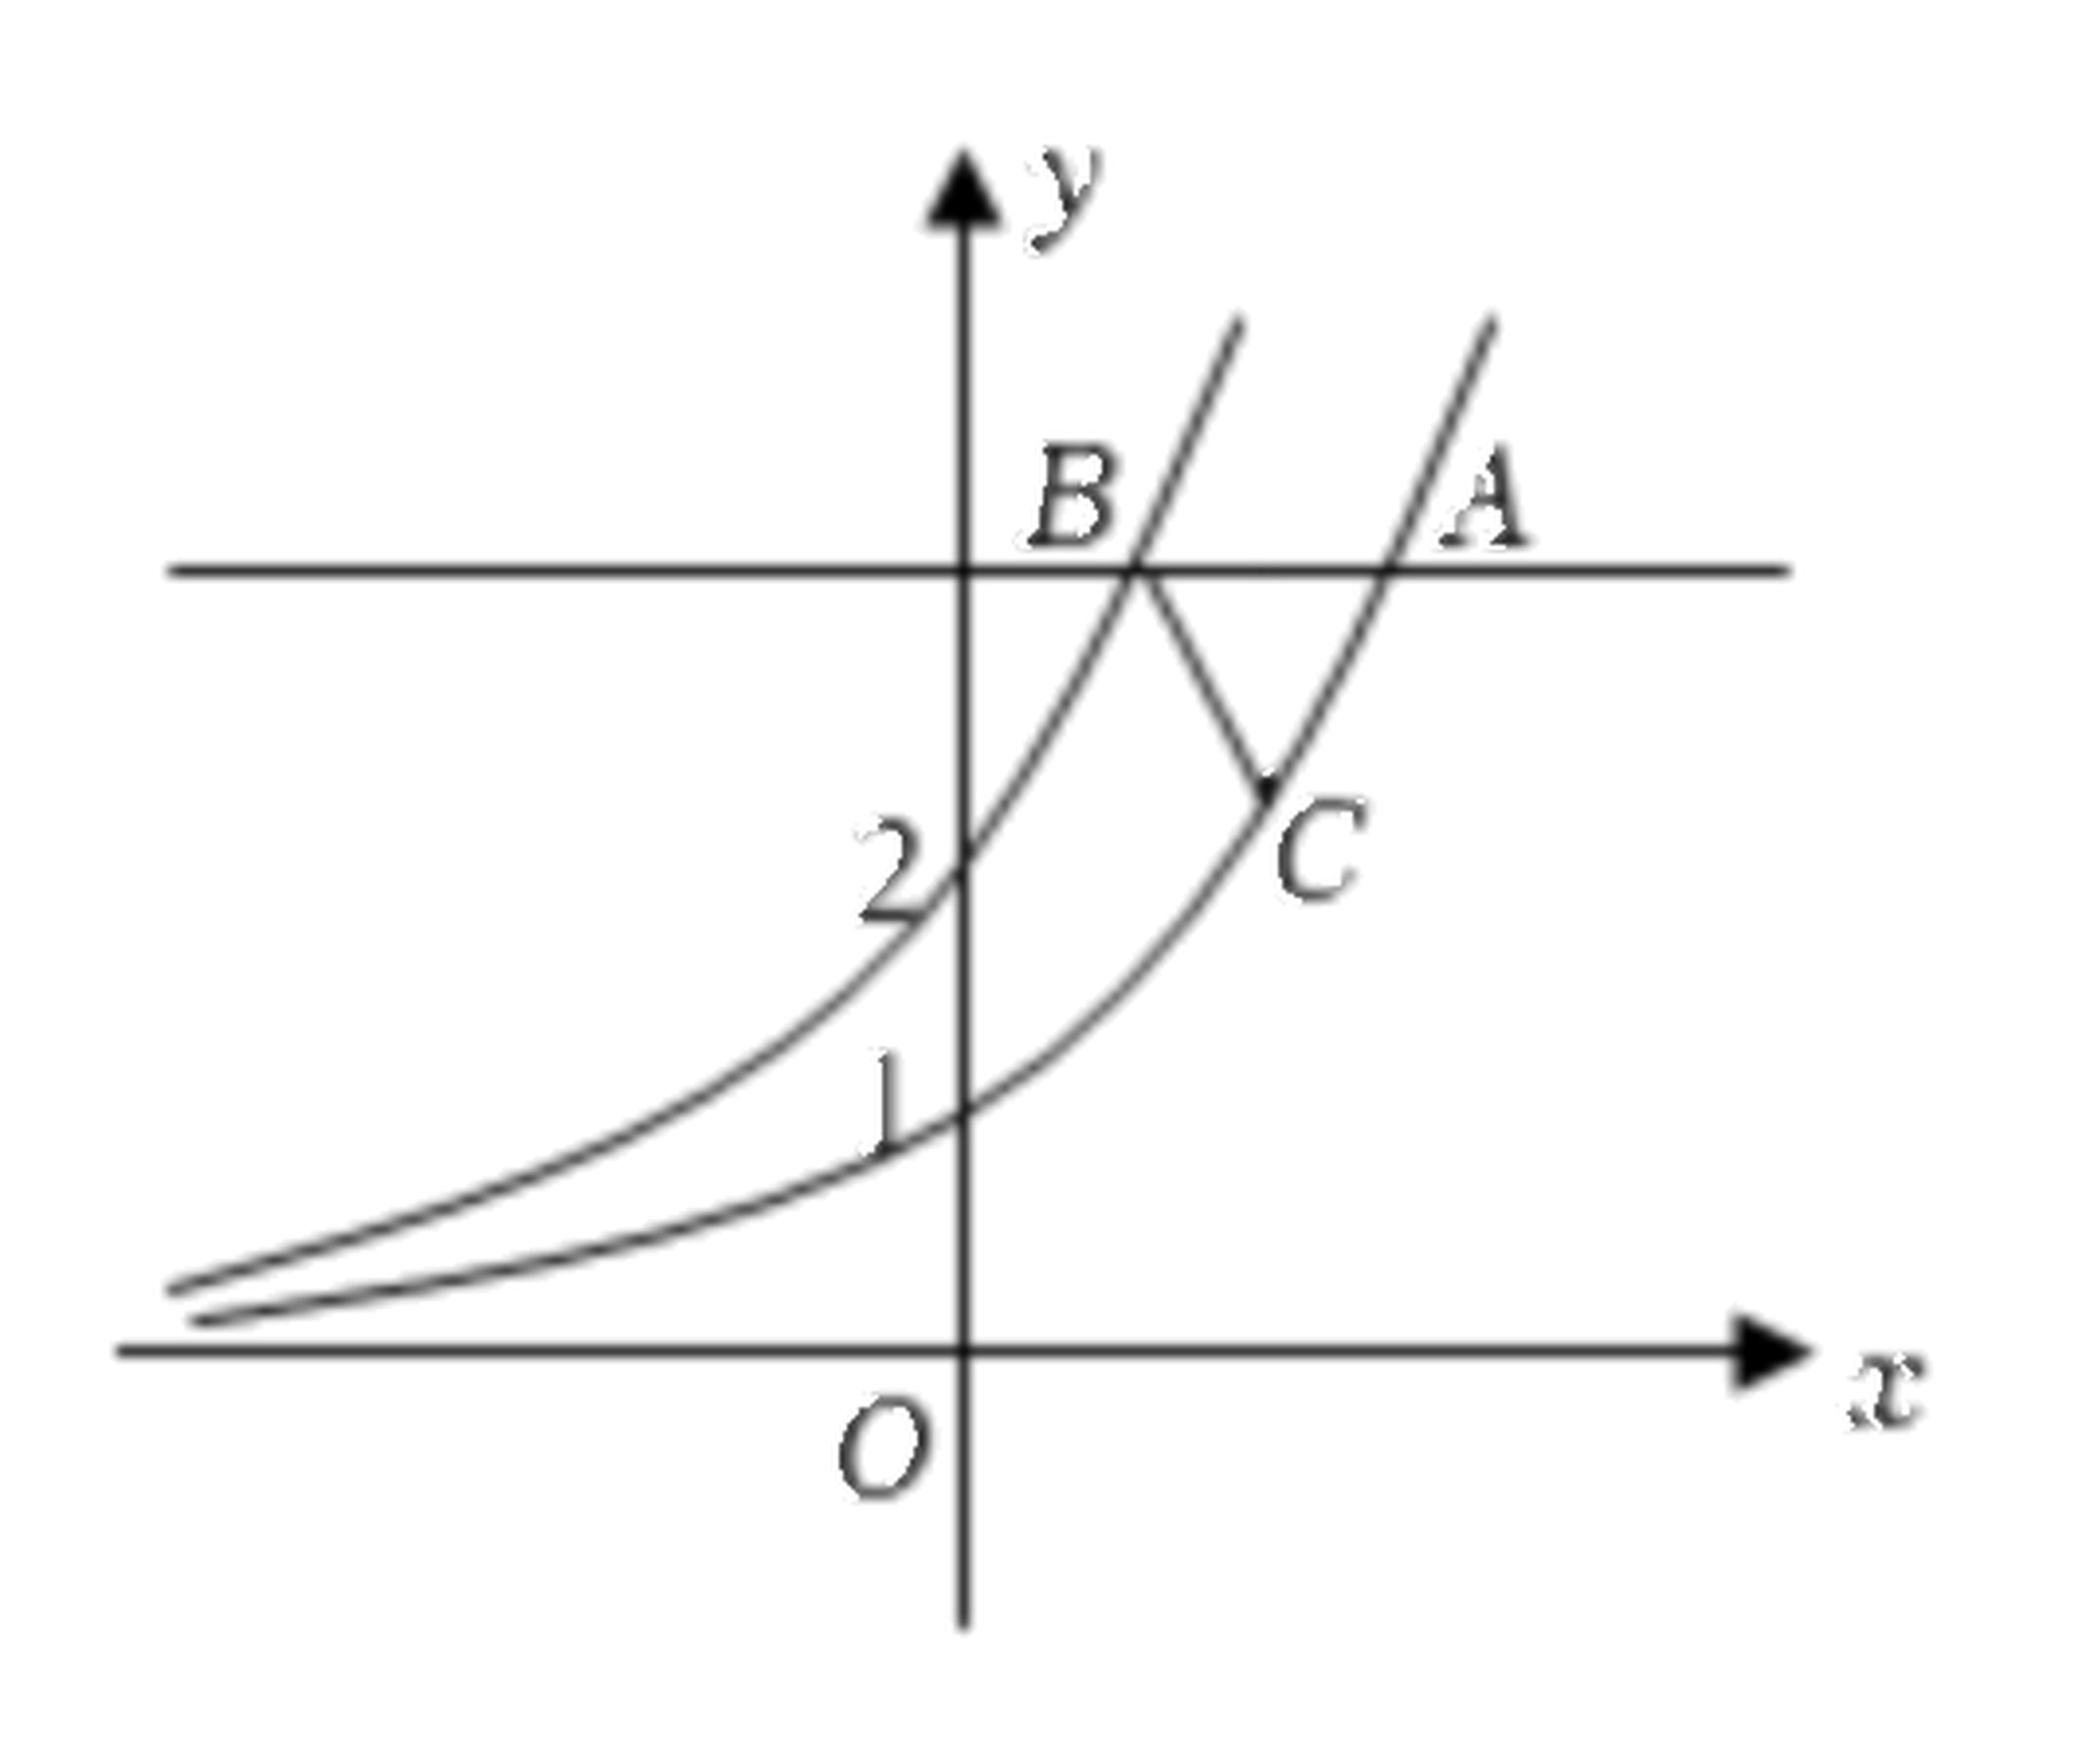
\includegraphics[width=0.40\textwidth]{figures/gao150_q11.png}
\end{center}

\ifanswer
\solbegin
\step{设直线 $l$ 的方程为 $y=a(a>0)$，}
\step{由 $2^x=a$，得 $x=\log_2 a$，所以 $A(\log_2 a,a)$，}
\step{由 $2^{x+1}=a$，得 $x=\log_2 a-1$，所以 $B(\log_2 a-1,a)$，所以 $\lvert AB\rvert=1$，}
\step{取 $AB$ 的中点 $D$，连接 $CD$，如图所示，}
\step{因为 $\triangle ABC$ 为等边三角形，则 $CD\perp AB$，且 $\lvert CD\rvert=\dfrac{\sqrt3}{2}$，}
\step{所以 $C\left(\log_2 a-\dfrac{1}{2},a-\dfrac{\sqrt3}{2}\right)$，}
\step{因为点 $C$ 在函数 $y=2^x$ 的图像上，所以 $a-\dfrac{\sqrt3}{2}=2^{\log_2 a-\frac{1}{2}}=\dfrac{a}{\sqrt2}$，}
\step{解得 $a=\dfrac{\sqrt3}{2-\sqrt2}=\dfrac{\sqrt3(2+\sqrt2)}{4-2}=\sqrt3+\dfrac{\sqrt6}{2}$，}
\step{所以点 $C$ 的纵坐标为 $a-\dfrac{\sqrt3}{2}=\dfrac{\sqrt3+\sqrt6}{2}$.}
\solend
\fi

% === Q12 === 解析配图（高斯函数方格阴影，仅答案版出）；"数学王子"弯引号；cases 块整体算一个印刷行；解析 4 行
\item 小玲在研究数学发展史，特别崇拜近代数学奠基者之一、享有“数学王子”称号的德国数学家高斯. 为了纪念高斯，我们把取整函数 $y=[x]$ 称为高斯函数，其中 $[x]$ 表示不超过 $x$ 的最大整数，如 $[1.1]=1$，$[-1.1]=-2$，则点集 $P=\{(x,y)\mid [x]^2+[y]^2=1\}$ 所表示的平面区域的面积为\blankline[4.4em].

\ifanswer
\solbegin
\step{$[x]^2+[y]^2=1$ 由 $\begin{cases}[x]=0\\ {[y]=-1}\end{cases}$ 或 $\begin{cases}[x]=0\\ {[y]=1}\end{cases}$ 或 $\begin{cases}[x]=-1\\ {[y]=0}\end{cases}$ 或 $\begin{cases}[x]=1\\ {[y]=0}\end{cases}$ 四个平面区域组成，}
\step{即 $\begin{cases}0\leqslant x<1\\ -1\leqslant y<0\end{cases}$ 或 $\begin{cases}0\leqslant x<1\\ 1\leqslant y<2\end{cases}$ 或 $\begin{cases}-1\leqslant x<0\\ 0\leqslant y<1\end{cases}$ 或 $\begin{cases}1\leqslant x<2\\ 0\leqslant y<1\end{cases}$，}
\step{作出平面区域如图所示，平面区域由四个边长为 $1$ 的正方形组成，}
\begin{center}
% 高斯函数 [x]^2+[y]^2=1 方格阴影区域图取 04 页顶部，去粉色水印、去色、4× LANCZOS 放大；仅答案版出
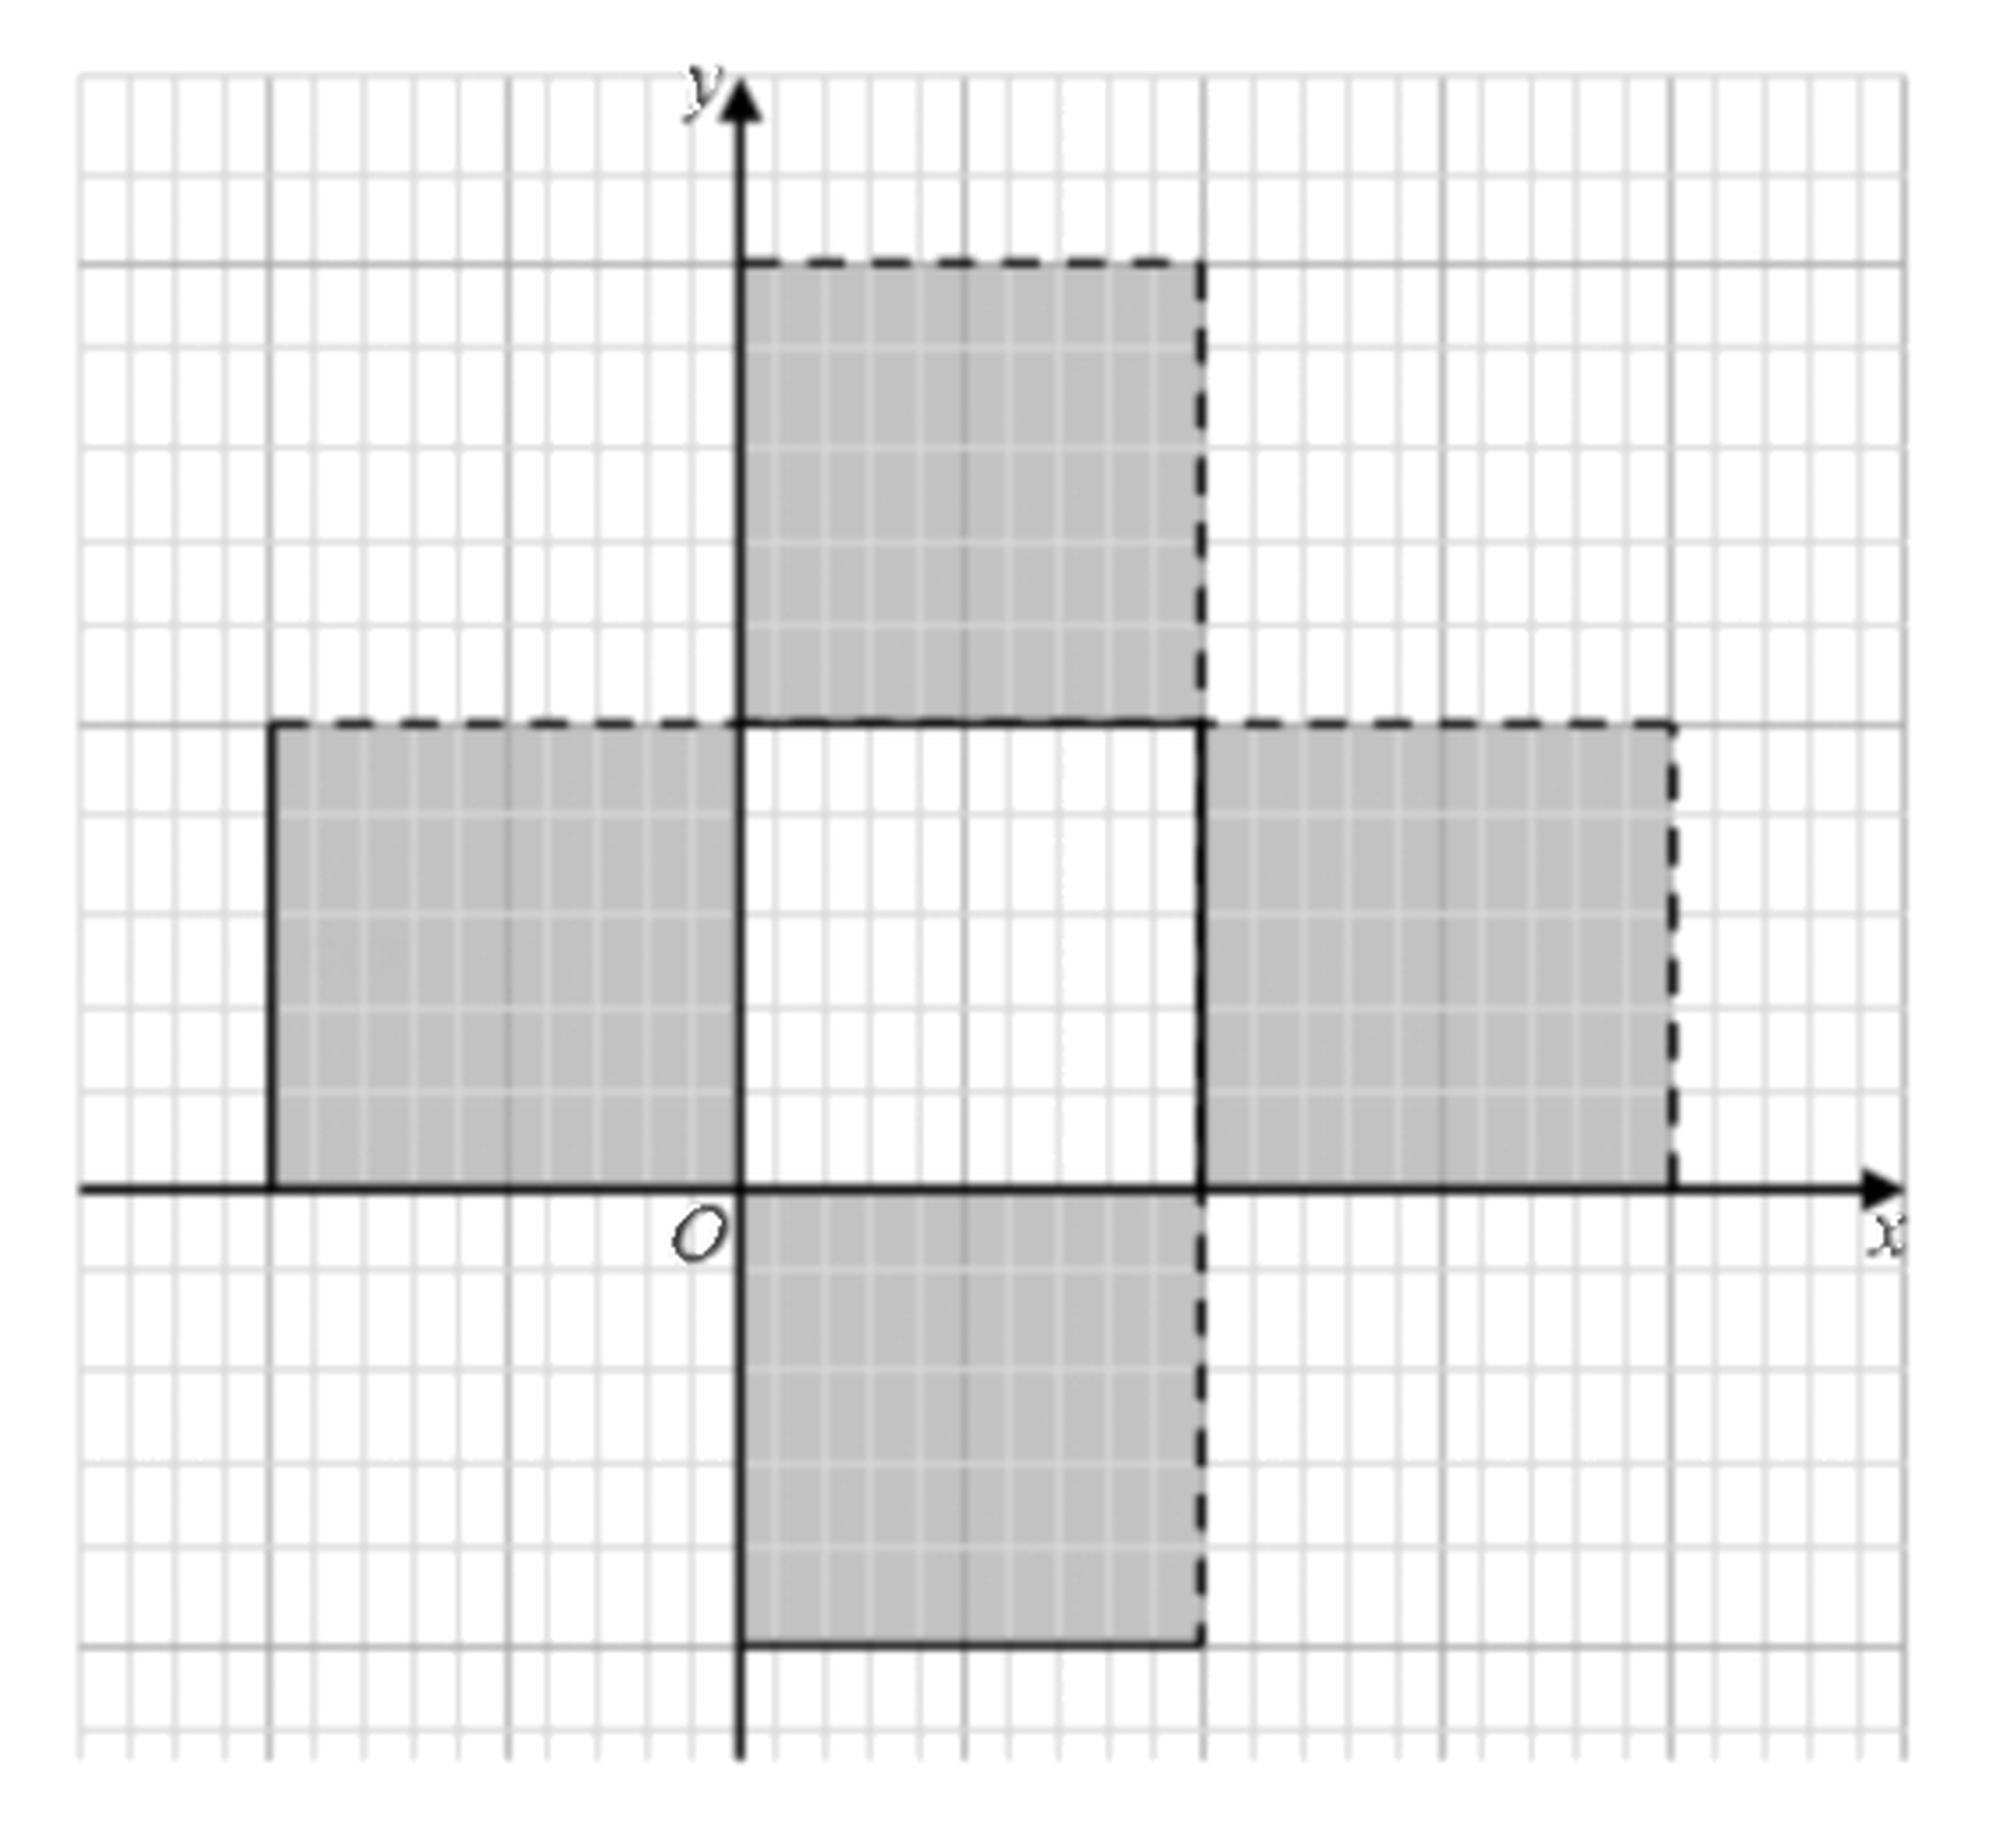
\includegraphics[width=0.34\textwidth]{figures/gao150_q12.png}
\end{center}
\step{总面积为 $1\times4=4$.}
\solend
\fi

\end{enumerate}

\bigsec{二、选择题}

\begin{enumerate}
\setcounter{enumi}{12}

% === Q13 === 答案在解析末句"故选 C"；括号 \mbox{（\quad）} 留空；四选项一行；解析 1 行
\item 设 $x\ne0$，则 $3^{\log_9 x^2}$ 的化简结果是\mbox{（\quad）}

\keepwithprev
A. $x$\qquad B. $\dfrac{1}{x}$\qquad C. $\lvert x\rvert$\qquad D. $\dfrac{1}{\lvert x\rvert}$

\ifanswer
\solbegin
\step{$3^{\log_9 x^2}=3^{\log_3\lvert x\rvert}=\lvert x\rvert$，故选 $C$.}
\solend
\fi

% === Q14 === 题目配图（两函数图像，三版都出）；\needvspace{8cm} 守卫放 \item 之前；"图像"照录；四选项两行两列；解析 2 行，故选 B
\needvspace{8cm}
\item 设 $a>0$ 且 $a\ne1$，$b\in\R$. 若函数 $y=a^{-\lvert x\rvert}$ 与 $y=x^b$ 的大致图像如图所示，则\mbox{（\quad）}

\keepwithprev
A. $0<a<1<b$\qquad\qquad B. $a>1$ 且 $b>1$

C. $0<a<1$ 且 $0<b<1$\qquad\qquad D. $0<b<1<a$

\begin{center}
% 两函数 y=a^{-|x|} 与 y=x^b 大致图像取 04 页右侧，去粉色水印、去色、4× LANCZOS 放大；三版都出
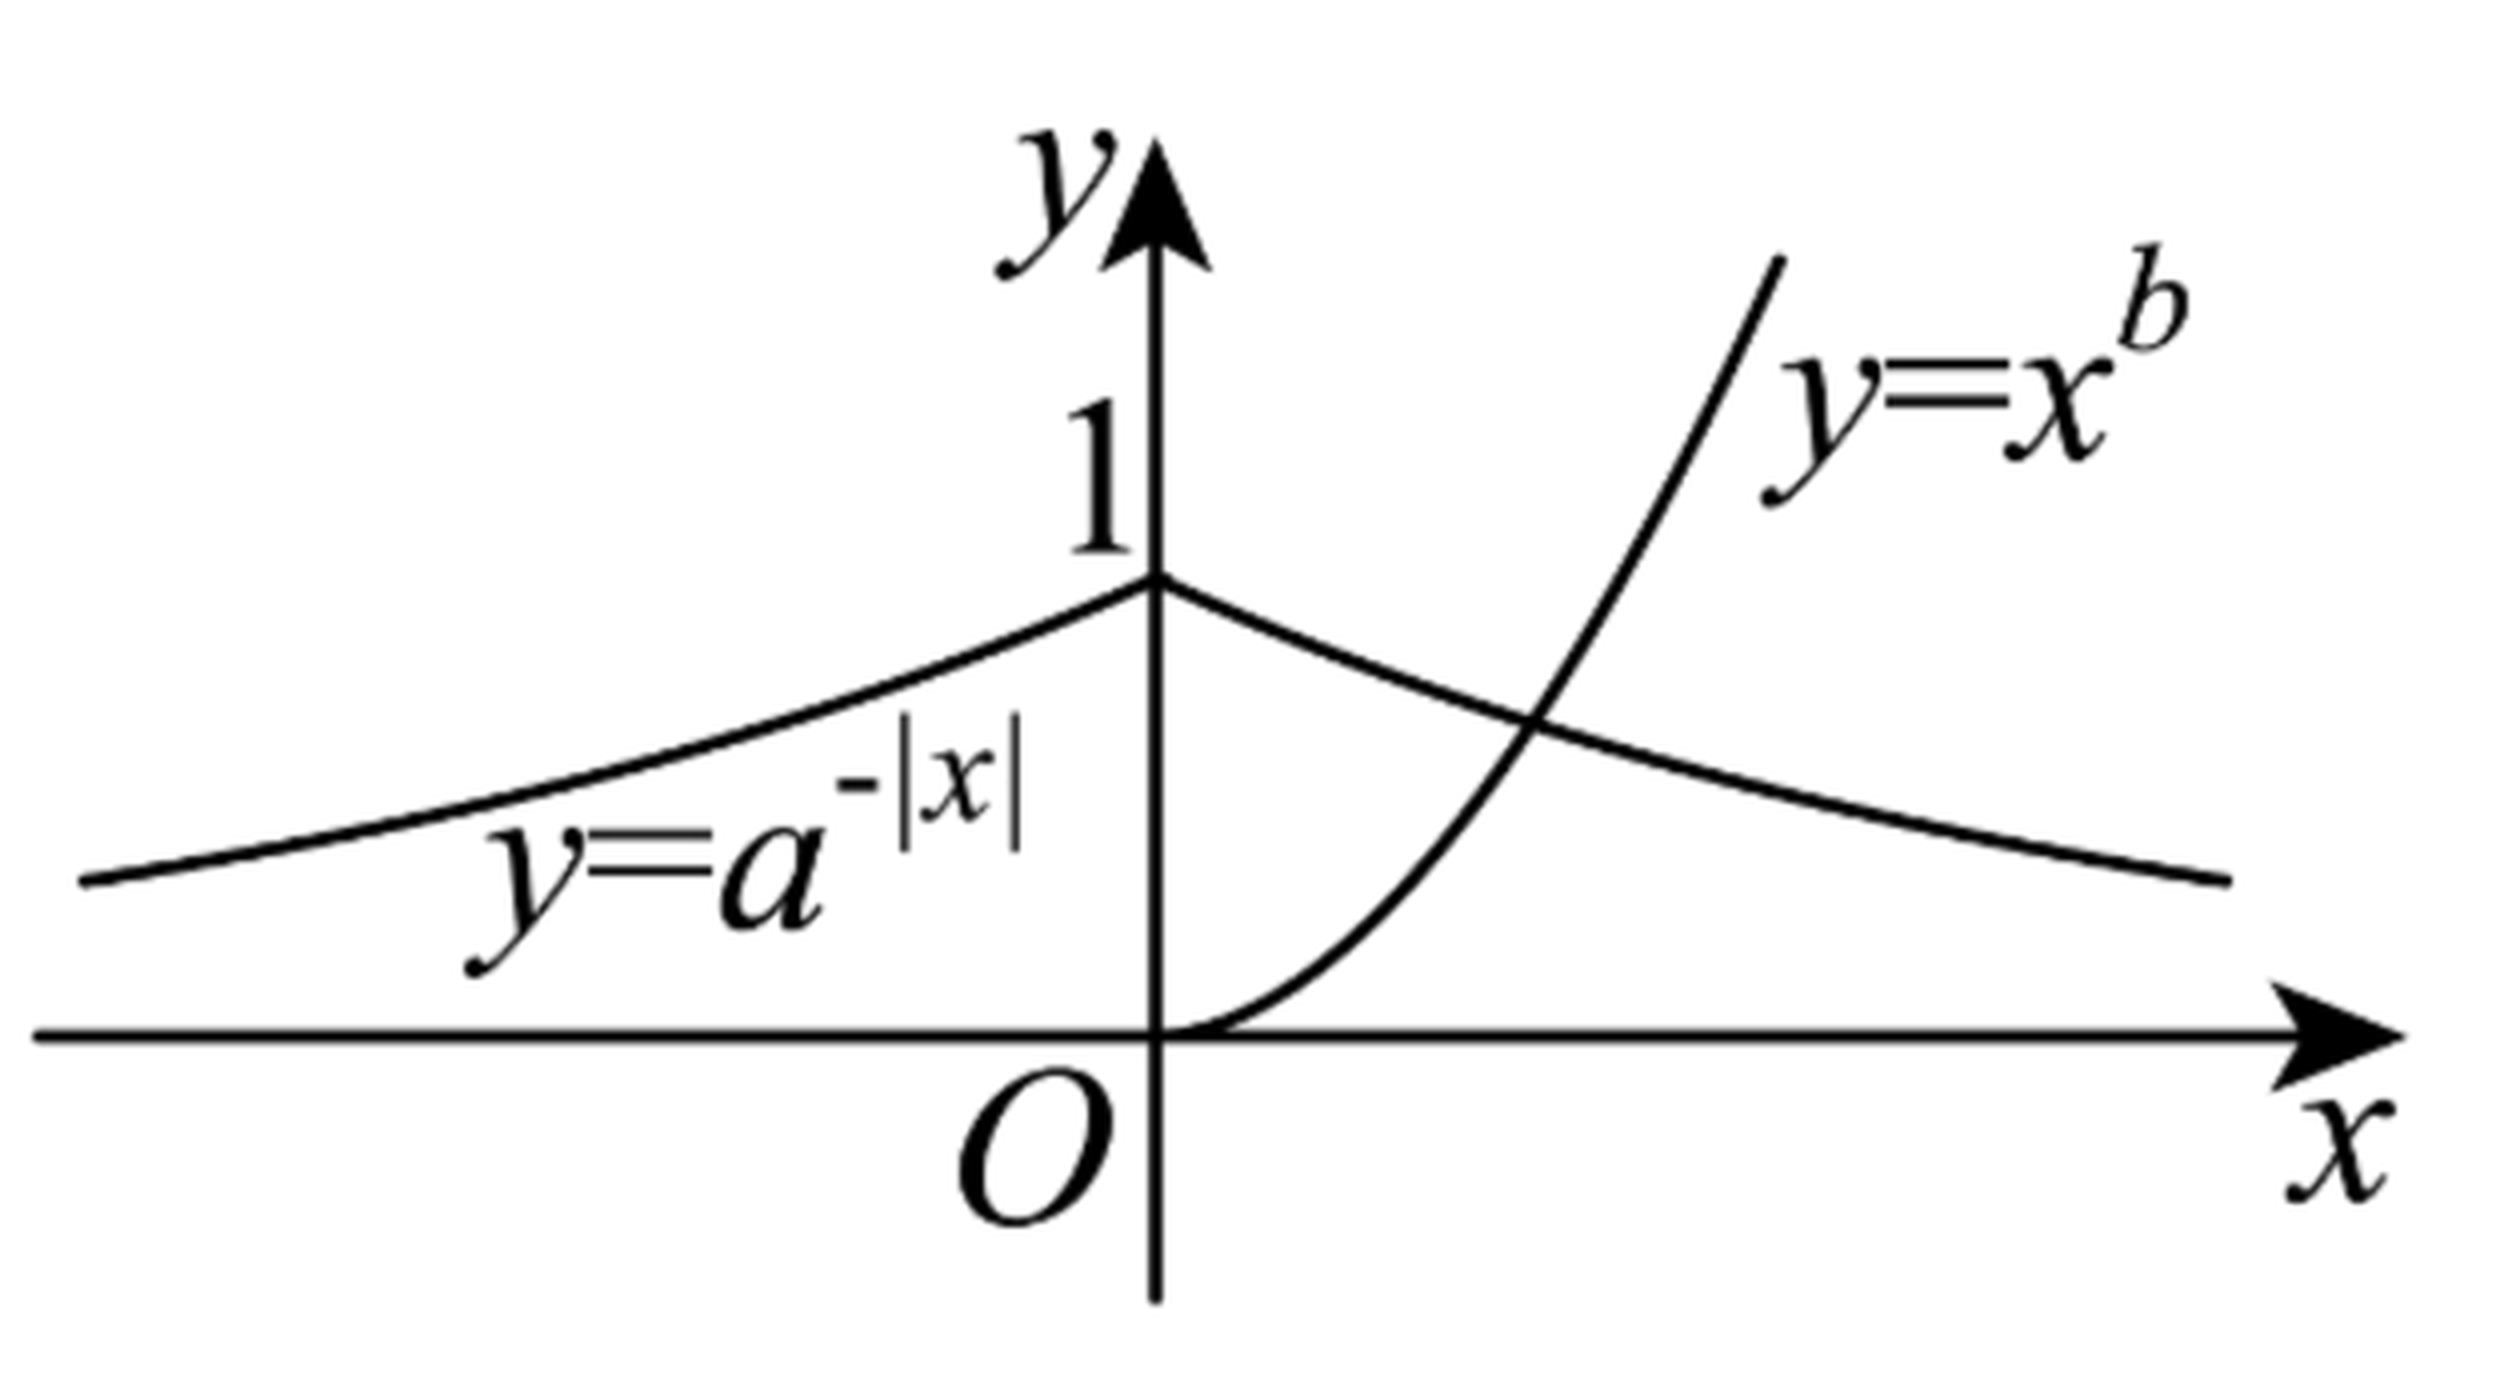
\includegraphics[width=0.40\textwidth]{figures/gao150_q14.png}
\end{center}

\ifanswer
\solbegin
\step{在 $(0,+\infty)$ 上，$y=a^{-x}$ 严格递减，得 $a>1$；}
\step{幂函数 $y=x^b$ 的图像递增且向上弯曲，得 $b>1$；故选 $B$.}
\solend
\fi

% === Q15 === "算术平均值／算术平均数"两处不同照录；四选项两行两列；解析 5 行（续 05 页顶），故选 B
\item 已知两个正数的算术平均值不小于它们的几何平均值，类比有以下结论：三个正数的算术平均数不小于它们的几何平均数，即当 $a,b,c$ 为正实数时，$\dfrac{a+b+c}{3}\geqslant\sqrt[3]{abc}$，当且仅当 $a=b=c$ 时等号成立. 利用上述结论，下列选项中判断正确的是\mbox{（\quad）}

\keepwithprev
A. 若 $x>0$，则 $2x+\dfrac{1}{x^2}\geqslant\dfrac{27}{8}$\qquad\qquad B. 若 $x>0$，则 $x^2+\dfrac{2}{x}\geqslant3$

C. 若 $0<x<1$，则 $x^2(1-x)\geqslant\dfrac{1}{9}$\qquad\qquad D. 若 $0<x<1$，则 $x^2(1-x)\leqslant\dfrac{1}{9}$

\ifanswer
\solbegin
\step{A：取 $x=1$，$2x+\dfrac{1}{x^2}=3<\dfrac{27}{8}$，错误.}
\step{B：$x^2+\dfrac{2}{x}=x^2+\dfrac{1}{x}+\dfrac{1}{x}\geqslant3\sqrt[3]{x^2\cdot\dfrac{1}{x}\cdot\dfrac{1}{x}}=3$，当且仅当 $x=1$ 时取等号，正确.}
\step{C：取 $x=\dfrac{1}{3}$，$x^2(1-x)=\dfrac{2}{27}<\dfrac{1}{9}$，错误.}
\step{D：取 $x=\dfrac{2}{3}$，$x^2(1-x)=\dfrac{4}{27}>\dfrac{1}{9}$，错误.}
\step{故选 $B$.}
\solend
\fi

% === Q16 === "完美集"新定义（弯引号、引号外空格照录）；圈数字①②文本模式；$n\in\N$；四选项两行两列；解析 9 行（6 行 05 页＋3 行 06 页顶），故选 A
\item 已知有限集 $A=\{a_1,a_2,\cdots,a_n\}$（$n\geqslant2$，$n\in\N$）. 若 $A$ 中元素 $a_i$（$i=1,2,\cdots,n$）满足 $a_1+a_2+\cdots+a_n=a_1\cdot a_2\cdots a_n$，就称 $A$ 为 “完美集”. 现有以下两个命题：

①恰有两个元素的 “完美集” 有无穷多个；

②若 $a_i$ 均为正整数，则 “完美集” $A$ 有且只有一个，且 $n=3$.

则\mbox{（\quad）}

\keepwithprev
A. ①和②都是真命题\qquad\qquad B. ①和②都是假命题

C. ①是真命题，②是假命题\qquad\qquad D. ①是假命题，②是真命题

\ifanswer
\solbegin
\step{①由 $a+b=ab\Leftrightarrow(a-1)(b-1)=1$，任取 $a>2$，则 $b=1+\dfrac{1}{a-1}\in(1,2)$，}
\step{得到无穷多个不同的完美集，①真.}
\step{②设 $1\leqslant a_1<a_2<\cdots<a_n$，则 $a_i\geqslant i$.}
\step{若 $n=2$，则 $(a_1-1)(a_2-1)=1$，只能有 $a_1=a_2=2$，与元素互异矛盾.}
\step{若 $n\geqslant4$，则 $a_1a_2\cdots a_n\geqslant a_2a_{n-1}a_n\geqslant2(n-1)a_n>na_n\geqslant a_1+\cdots+a_n$，矛盾.}
\step{当 $n=3$ 时，若 $a_1\geqslant2$，则 $a_1a_2a_3\geqslant6a_3>3a_3\geqslant a_1+a_2+a_3$，矛盾.}
\step{因此 $a_1=1$，$(a_2-1)(a_3-1)=2$，结合 $a_2<a_3$ 得 $a_2=2$，$a_3=3$.}
\step{唯一的完美集为 $\{1,2,3\}$，②真.}
\step{故选 $A$.}
\solend
\fi

\end{enumerate}

\bigsec{三、解答题}

\begin{enumerate}
\setcounter{enumi}{16}

% === Q17 === \varnothing 空集、$B\subseteq A$ 带下划线照录；弯引号内空格照录；解析 7 行
\item 设 $a,b\in\R$. 已知集合 $A=\{x\mid ax^2+3x-a>3\}$，$B=\{x\mid bx=1\}$.

(1) 若 $A=(1,2)$，求 $a$ 的值；

(2) 若 $a=0$，且 “ $x\in A$ ” 是 “ $x\in B$ ” 的必要非充分条件，求 $b$ 的取值范围.

\ifanswer
\solbegin
\step{(1) $A=(1,2)$，则 $a<0$，且 $1,2$ 是方程 $ax^2+3x-a-3=0$ 的两根.}
\step{由 $4a+6-a-3=0$，得 $a=-1$，此时不等式为 $-(x-1)(x-2)>0$，}
\step{解集确为 $(1,2)$.}
\step{(2) $a=0$ 时，$A=(1,+\infty)$，题意等价于 $B\subseteq A$ 且 $B\ne A$.}
\step{当 $b=0$ 时，$B=\varnothing$，符合条件.}
\step{当 $b\ne0$ 时，$B=\left\{\dfrac{1}{b}\right\}$，条件等价于 $\dfrac{1}{b}>1$，解得 $0<b<1$.}
\step{因此 $b$ 的取值范围为 $[0,1)$.}
\solend
\fi

% === Q18 === $p\in\Z$；"图像"（像，有亻）照录；指数 $-2p^2+5p$；解析 8 行（(1) 首行 06 页末＋2 行 07 页顶、(2) 5 行 07 页）
\item 设 $p\in\Z$，已知 $f(x)=x^{-2p^2+5p}$.

(1) 若幂函数 $y=f(x)$ 的图像关于原点成中心对称，且满足 $f(3)<f(4)$，求 $p$ 的值；

(2) 当 $p=-2$ 时，求满足 $f(2x+3)<f(x-4)$ 的 $x$ 的取值范围.

\ifanswer
\solbegin
\step{(1) 图像关于原点成中心对称，得整数 $-2p^2+5p$ 为奇数.}
\step{由 $f(3)<f(4)$，得 $-2p^2+5p>0\Leftrightarrow0<p<\dfrac{5}{2}$，}
\step{结合 $p\in\Z$，得 $p=1$ 或 $p=2$，对应指数分别为 $3$、$2$，所以 $p=1$.}
\step{(2) 当 $p=-2$ 时，$f(x)=\dfrac{1}{x^{18}}$，定义域为 $\{x\in\R\mid x\ne0\}$.}
\step{原不等式要求 $x\ne-\dfrac{3}{2}$ 且 $x\ne4$，}
\step{此时 $\dfrac{1}{(2x+3)^{18}}<\dfrac{1}{(x-4)^{18}}\Leftrightarrow\lvert 2x+3\rvert>\lvert x-4\rvert\Leftrightarrow(2x+3)^2>(x-4)^2$，}
\step{因此 $(x+7)(3x-1)>0\Leftrightarrow x<-7$ 或 $x>\dfrac{1}{3}$，}
\step{排除 $x=4$，得 $x\in(-\infty,-7)\cup\left(\dfrac{1}{3},4\right)\cup(4,+\infty)$.}
\solend
\fi

% === Q19 === $a\in\R$、$g(x)=f(2x+1)+a\cdot f(x)+2$；解析 6 行（(2) 末两行续 08 页顶）
\item 已知 $f(x)=2^x$.

(1) 求方程 $f(2x)-f(x)=6$ 的解；

(2) 设 $a\in\R$，$g(x)=f(2x+1)+a\cdot f(x)+2$，若对于任意 $x\in[-1,1]$，均有 $g(x)\geqslant1$，求 $a$ 的取值范围.

\ifanswer
\solbegin
\step{(1) 令 $t=2^x>0$，则 $t^2-t-6=(t-3)(t+2)=0$，}
\step{由 $t>0$ 得 $t=3$，所以 $x=\log_2 3$.}
\step{(2) 令 $t=2^x$，则 $t\in\left[\dfrac{1}{2},2\right]$，且 $g(x)\geqslant1\Leftrightarrow2t^2+at+1\geqslant0\Leftrightarrow a\geqslant-\left(2t+\dfrac{1}{t}\right)$，}
\step{由基本不等式得 $2t+\dfrac{1}{t}\geqslant2\sqrt{2t\cdot\dfrac{1}{t}}=2\sqrt2$，}
\step{当且仅当 $t=\dfrac{1}{\sqrt2}\in\left[\dfrac{1}{2},2\right]$ 时等号成立，}
\step{因此 $-\left(2t+\dfrac{1}{t}\right)$ 的最大值为 $-2\sqrt2$，所求范围为 $a\in[-2\sqrt2,+\infty)$.}
\solend
\fi

% === Q20 === "极闭集"新定义、3 问，全卷末题；$M\subseteq(0,+\infty)$ 带下划线照录；自定义运算 $x*y$ 星号照录；解析 13 行（9 行 08 页＋4 行 09 页上半）
\item 对于非空实数集 $M\subseteq(0,+\infty)$，若满足以下两个条件：

① $M$ 中至少含有 $2$ 个元素，且 $1\notin M$；

②对于 $M$ 中任意两个不相等的元素 $x$、$y$，定义 $x*y=\dfrac{xy+1}{x+y}$，且 $x*y\in M$.

则称 $M$ 为 “极闭集”.

(1) 分别判断集合 $A=\left\{\dfrac{1}{2},3\right\}$ 与集合 $B=(1,+\infty)$ 是否为 “极闭集” （无需理由）；

(2) 若 $M$ 是 “极闭集”，证明：$M$ 中不可能所有元素都小于 $1$；

(3) 证明：不存在任何有限集是 “极闭集”.

\ifanswer
\solbegin
\step{(1) $A$ 不是 “极闭集”，$B$ 是 “极闭集”.}
\step{(2) 假设 $M$ 中所有元素都小于 $1$，取其中两个不相等的元素 $x$、$y$，}
\step{则 $x*y-1=\dfrac{(1-x)(1-y)}{x+y}>0$，}
\step{这与 $x*y\in M$ 且 $M$ 中所有元素都小于 $1$ 矛盾.}
\step{(3) 假设有限集 $M$ 是 “极闭集”，}
\step{由 (2) 及 $1\notin M$，得 $M$ 中存在大于 $1$ 的元素.}
\step{若 $M$ 中有小于 $1$ 的元素，取其中最大的一个为 $a$，另取 $b\in M$ 且 $b>1$，}
\step{则 $a*b-a=\dfrac{1-a^2}{a+b}>0, a*b-1=\dfrac{(a-1)(b-1)}{a+b}<0$，}% 半角逗号在两个数学式组之间，全稿惯例、非笔误，照录
\step{于是 $a<a*b<1$ 且 $a*b\in M$，与 $a$ 的最大性矛盾.}
\step{若 $M$ 中没有小于 $1$ 的元素，则 $M\subseteq(1,+\infty)$.}
\step{取 $a=\min M$，另取 $b\in M$ 且 $b\ne a$，则 $a*b-a=\dfrac{1-a^2}{a+b}<0$，}
\step{于是 $a*b<a$ 且 $a*b\in M$，与 $a$ 的最小性矛盾.}
\step{因此不存在任何有限集是 “极闭集”.}
\solend
\fi

\end{enumerate}

\end{document}
"
%
% ① 原始材料：微信公众号"魔都数学加油站"文章，连载"27学年高一150"，原文标题
% "27学年高一150——2026-2027年上海市曹杨二中高一上期中"；
% 原文链接：https://mp.weixin.qq.com/s/xlQxmik8TZXR87RC6MnCrw 。
% 正文为 9 张 PNG 页（01/02/04/06/07/09 为 2560×3620，03/05/08 为 4762×6735，
% 同一篇各页分辨率混排，逐页按各自分辨率裁图核对，别按预览比例换算裁框）。
% 体例：讲评版——全 18 题均印【解析】（逐题核实，见 ② ②）。
% 题目、答案、解析均据原图转录；卷面粉红色/红色水印"魔都数学加油站"及公众号页脚未录入。
% 全卷插图清单（逐页通读 9 页确认）：3 幅——
%   · Q11 题目配图（指数函数曲线图，02 页右侧：x/y 轴、O、y=2^x 与 y=2^{x+1}
%     两曲线、A/B/C 三点、刻度 1/2、等边三角形 ABC），三版都出，裁 figures/gao150_q11.png；
%   · Q12 解析配图（高斯函数取整 [x]^2+[y]^2=1 方格阴影区域图，04 页顶部：4 个边长 1
%     的正方形组成的十字形阴影），解析"作出平面区域如图所示"处，仅答案版出，
%     放 \ifanswer 内 \step 之间，裁 figures/gao150_q12.png；
%   · Q14 题目配图（两函数 y=a^{-|x|} 与 y=x^b 大致图像，04 页右侧：x/y 轴、O、
%     y 轴刻度 1、一递减曲线一递增上翘曲线），三版都出，裁 figures/gao150_q14.png；
%   其余各页逐页确认无其它题目配图、无表格；Q11/Q12 解析"如图所示"对应的就是上列
%   已裁的图，不重复裁；09 页上半为 Q20(3) 解析续尾、下半仅水印、无正文。
%   3 图均取自原卷截图，去粉色水印、去色、4× LANCZOS 放大。
%
% 卷首标题：原卷印作"2026-2027 年曹杨二中高一上期中"，年份区间按全稿惯例排 en dash；
% 原卷卷面未印副标题，本稿按同期中卷知识模块口径补出"集合与常用逻辑用语、不等式、函数"。
%
% 题号体例（逐页核实定稿）：本卷共 18 题——一、填空题 3—12（10 题）、
% 二、选择题 13—16（4 题）、三、解答题 17—20（4 题）。
% 三节分别 \setcounter{enumi}{2}／{12}／{16}。原卷从第 3 题起、无第 1、2 题，
% 本稿保留原题号；全卷末题为第 20 题（"极闭集"新定义、3 问），无 Q21、无附加题节。
%
% ② 与原卷的排版差异：
%   ① 原文从第 3 题起，本稿保留原题号；共 18 题三节，解答题只有 4 题到 20；
%   ② 全 18 题均印【解析】，用 \solbegin…\solend；逐题核实无只印【答案】或
%      答案印题干括号内的题；四道选择题答案在解析末句"故选 X"（Q13 选 C、
%      Q14 选 B、Q15 选 B、Q16 选 A，逐个放大复核）、括号 \mbox{（\quad）} 留空、
%      不另提 \ans{}；答案版【答案】/【解析】标记数 = 18 = 全卷题数；
%   ③ 原卷卷面未印副标题，本稿按知识模块口径补出；
%   ④ 原卷填空横线按全稿惯例排 \blankline[4.4em]；选择题括号排 \mbox{（\quad）}、
%      选项段前按惯例加 \keepwithprev；解答题不留作答区、不加 \anspace（原卷为讲评版）；
%   ⑤ 数集黑板粗体：Q4"m\in R"、Q5"a,b\in R"、Q6"a,b,c\in R"、Q7"a\in R"、
%      Q10"a\in R"、Q14"b\in R"、Q17"a,b\in R"、Q18"p\in Z"／定义域"x\in R"、
%      Q19"a\in R"、Q16"n\in N" 原卷印斜体 R/Z/N，按全稿惯例归一 \R／\Z／\N；
%      绝对值排 \lvert…\rvert（Q7 |x+4|+|x-3|、Q11 |AB|／|CD|、Q13 |x|、
%      Q18 |2x+3|／|x-4|），集合描述竖线排 \mid（Q3、Q12、Q17、Q18、Q20），
%      不等号按全稿惯例排 \leqslant／\geqslant；补集照原卷上划线排 \overline{A}
%      （Q3 题干＋解析共 2 处）；空集符号 \varnothing（Q17 解析(2)）；
%      子集 \subset（单线⊂）／\subseteq（带下划线⊆）逐处照录，本卷 3 处子集
%      符号均印带下划线 ⊆、照录 \subseteq（Q20 题干、Q20 解析(3)、Q17 解析(2)，
%      见 ④），无 \subset 用例；
%   ⑥ 判别式 Δ/△：逐页通读 9 页，本卷无一元二次判别式算式，故无 Δ/△ 混用可照录
%      （"高 \Delta／扁 \triangle"口径备查，参照 高一142／144／145／146／148／149
%      头注④）；本卷仅 Q11 题干与解析共 2 处几何三角形符号 △ABC，逐处放大并排
%      确认两处同形、印近等边粗线三角（非判别式），照录 \triangle（见 ④）；
%   ⑦ 中文弯引号照录：Q12"数学王子"、Q16"完美集"（题干＋①②两命题，引号外
%      留空格）、Q17" x∈A "" x∈B "（引号内空格）、Q20"极闭集"（题干条件、
%      三问与解析，引号外留空格）；注释里一律 ASCII 引号；数学式内 CJK 用 \text{}
%      （Q3 集合描述"且"用 \text{ 且 }）；
%   ⑧ 半角逗号在数学组之间是全稿惯例、非笔误，逐处照录（Q17 解析"1,2 是方程…
%      两根"、Q20 解析(3)">0, a*b-1=…<0" 两式之间等）；行末西文句点 ASCII `.`；
%      行中全角逗号／顿号照录（Q12"之一、享有"、Q18 解析"3、2"、Q20"x、y"）；
%   ⑨ "图像／图象"逐处放大核：全卷 9 处均印"图像"（像，有亻）、未见"图象"——
%      Q4 题干 1、Q11 题干 2＋解析 1、Q14 题干 1＋解析 1、Q18 题干 1＋解析 1；
%      同卷"第二象限""象限"用"象"（无亻）。逐处照录未统一改动（放大 01/02/04/06
%      页 /tmp/gao150/z/p01_q4_tuxiang2.png、p04_q14_tuxiang2.png、
%      p02_q11_lines.png 确认）；子题标号 (1)(2)(3) 半角括号照录；圈数字①②
%      在文本模式（Q16 两命题与解析、Q20 两条件与三问及解析）按 common.sty
%      划入 CJK 字符类渲染，进数学式用 \text{①}；
%   ⑩ Q20 新定义 x*y=\dfrac{xy+1}{x+y} 的 * 是自定义运算（星号），照录；
%      \left…\right 不得拆到不同 $…$ 组（Q19"\left(2t+\frac1t\right)"、
%      Q20 题干"A=\left\{\frac12,3\right\}"等）；Q8 嵌套根号
%      \sqrt{\frac2x+\frac{16}{1-2x}}、Q9 对数连加 \log_2 A 等复杂式照录别简化；
%   ⑪ 一条 \step = 原卷解析的一个印刷行，cases 块整体算一个印刷行；别并折行、
%      别拆行。Q4 三行、Q8 五行、Q11 九行、Q12 四行（两行各含四个 cases 块）、
%      Q15 五行、Q16 九行、Q18 八行、Q20 十三行均按印刷行逐条断，不丢行；
%   ⑫ 配图：Q11／Q14 题目配图（三版都出）放 \item 内题干之后 \begin{center}，
%      大图块加 \needvspace{8cm} 守卫把整块推走（守卫放 \item 之前，见
%      高一145 Q14/Q20 成例与切页审计 B 类坑）；Q12 解析配图（仅答案版出）
%      放 \ifanswer 内 \solbegin…\solend 的 \step 之间（高一73 第16题成例）；
%   ⑬ 跨页续印按题合并：见 ⑥；
%   ⑭ 原卷解析内无红色"法一／法二"之类小标题，故本卷无 \stepm；红色水印
%      "魔都数学加油站"不录入；Q12 解析"作出平面区域如图所示"对应的图即
%      ① 所列 gao150_q12.png（04 页顶部），不重复裁；Q11 解析"如图所示"对应
%      题目配图 gao150_q11.png，不另裁。
%
% ③ 行数复核：一条 \step／\stepm = 原卷解析的一个印刷行，cases 块作一个印刷行计。
%   逐题数（主会话逐页核对定稿）：Q3：1；Q4：3；Q5：2；Q6：1；Q7：2；Q8：5；
%   Q9：1；Q10：3；Q11：9；Q12：4；Q13：1；Q14：2；Q15：5；Q16：9；
%   Q17：7；Q18：8；Q19：6；Q20：13。
%   合计 82 条 \step（本卷无 \stepm：解析内无红色"法一／法二"类小标题），
%   与原卷逐题印刷行相等。全卷 18 题均设 \solbegin…\solend，答案版
%   【答案】/【解析】标记数 = 18 = 全卷题数。
%
% ④ 判别式／三角形／子集符号结论（逐处放大原图照录、不得统一，主会话像素级复核）：
%   判别式：逐页通读 9 页，本卷无一元二次判别式 Δ/△ 算式（Q18 讨论幂函数指数
%     奇偶、不用判别式；Q9／Q19／Q20 亦无），头注 ② ⑥ 的"高 \Delta／扁 \triangle"
%     口径在本卷无对应处（参照 高一142／144／145／146／148／149 头注④，仅备查）。
%   几何三角形符号：Q11 题干"使得 △ABC 为等边三角形"（02 页末）与解析
%     "因为 △ABC 为等边三角形，则 CD⊥AB"（03 页）共 2 处，放大 02/03 页
%     /tmp/gao150/z/q11_tri_montage2.png 并排确认两处同形、印近等边粗线三角
%     （h/w≈0.98、非"高>宽"的判别式 \Delta），照录 \triangle（与 高一105
%     "使得 \triangle ABC 为等边三角形" 同短语成例、高一149 几何三角形照录
%     \triangle 口径一致），不引入 \Delta。
%   子集／补集：Q20 题干"$M\subseteq(0,+\infty)$"（08 页）、Q20 解析(3)
%     "则 $M\subseteq(1,+\infty)$"（09 页）、Q17 解析(2)"题意等价于 $B\subseteq A$
%     且 $B\ne A$"（06 页）共 3 处子集符号，逐处放大（/tmp/gao150/z/p08_q20_stem.png、
%     p09_q20_sub.png、p06_q17_sub.png）确认均印带下划线 ⊆，照录 \subseteq；
%     本卷未见单线 ⊂（\subset）之对应处。Q3 题干与解析共 2 处补集照原卷上划线
%     排 \overline{A}；Q17 解析(2) 空集印 ∅、照录 \varnothing（Q7"解集为空集"
%     为中文词、非符号，照录文字）；集合描述竖线 \mid；数集 \R／\Z／\N 归一见 ② ⑤。
%
% ⑤ 存疑照录（放大原图确认，照录未改、正文对应处另有 % 注）：
%   1. Q8 解析第 4 行"所以 $y=\frac1x+\frac{8}{1-2x}$ 的最小值为 18" —— 上文
%      并未定义 $y$，且题面求的是 $\sqrt{\frac2x+\frac{16}{1-2x}}$ 的最小值；
%      按上下文该行应为 $\frac1x+\frac{8}{1-2x}$ 的最小值为 18（$y$ 疑为原卷
%      衍字／笔误），放大 02 页 /tmp/gao150/z/p02_q8_y.png 确认，照录未改。
%   2. Q20 解析(3)"$a*b-a=\frac{1-a^2}{a+b}>0, a*b-1=\frac{(a-1)(b-1)}{a+b}<0$"
%      两式之间的逗号原卷印半角 ,（非全角），按全稿惯例"半角逗号在数学组之间"
%      照录未改（放大 08 页 /tmp/gao150/z/p08_q20_sol8.png 确认）。
%   3. Q15 题干"两个正数的算术平均值…几何平均值"与"三个正数的算术平均数…
%      几何平均数"两处"值／数"用字不同，逐处照录未统一（放大 04 页确认）。
%   4. "图像／图象"全卷 9 处均印"图像"（像，有亻）、未见"图象"，逐处放大核实
%      照录、未统一改动（见 ② ⑨）；本卷判别式 Δ/△ 无用例、几何三角形 2 处
%      照录 \triangle（见 ④）。
%   全卷除此 4 类外未发现其它笔误／自相矛盾处；18 题均印【解析】、无只印【答案】
%   或答案印题干括号内的题（见 ② ②）。
%
% ⑥ 跨页续印按题合并说明（逐页核实定稿）：Q3/4/5/6/7 题干＋解析在 01 页；
%   Q8 题干＋解析 5 行、Q9 题干＋解析 1 行在 02 页上半；Q10 题干＋解析 3 行
%   在 02 页下半；Q11 题干（前两行）＋配图在 02 页下半、题干续"三角形，则点 C
%   的纵坐标为___"与解析 9 行全在 03 页上半（解析"如图所示"对应题目配图）；
%   Q12 题干＋解析 4 行在 03 页下半，解析配图（方格阴影）续印在 04 页顶部；
%   "二、选择题"标题在 04 页中部；Q13 题干＋选项＋解析、Q14 题干＋选项＋
%   配图＋解析在 04 页；Q15 题干＋四选项在 04 页末、解析 5 行续 05 页上半；
%   Q16 题干＋①②两命题＋"则(  )"＋四选项＋解析前 6 行在 05 页、解析末 3 行
%   （"因此 a_1=1…②真""故选 A"）续 06 页顶部；"三、解答题"标题在 06 页；
%   Q17 题干(1)(2)＋解析(1) 3 行＋解析(2) 首行在 06 页、解析(2) 续 3 行
%   在 06 页下半；Q18 题干(1)(2)＋解析(1) 首行在 06 页末、解析(1) 续 2 行＋
%   解析(2) 5 行在 07 页上半；Q19 题干(1)(2)＋解析(1) 2 行＋解析(2) 前 2 行
%   在 07 页下半、解析(2) 末 2 行续 08 页顶部；Q20 题干（新定义＋①②两条件）
%   ＋三问＋解析(1)(2)(3) 前 9 行在 08 页、解析(3) 末 4 行续 09 页上半，
%   末行"因此不存在任何有限集是极闭集"为全卷收尾（09 页下半仅水印、无正文）。
%   本稿按题连排，不丢行、不并折行；全卷末题为第 20 题，无 Q21、无附加题节。
%
\documentclass[a4paper,11pt]{article}
\usepackage{common}

\begin{document}

\examtitlest[3]{2026--2027 年曹杨二中高一上期中}{集合与常用逻辑用语、不等式、函数}

\bigsec{一、填空题}

\begin{enumerate}
\setcounter{enumi}{2}

% === Q3 === 补集上划线 \overline{A}（题干＋解析各 1 处）；集合描述竖线 \mid、数学式内"且"用 \text{}；解析 1 行
\item 设全集 $U=\{1,2,3,4,5\}$，集合 $A=\{x\mid x^2-3x\leqslant0\text{ 且 }x\in U\}$，则 $\overline{A}=$\blankline[4.4em].

\ifanswer
\solbegin
\step{$x^2-3x\leqslant0\Leftrightarrow0\leqslant x\leqslant3$，所以 $A=\{1,2,3\}$，$\overline{A}=\{4,5\}$.}
\solend
\fi

% === Q4 === "图像"（像，有亻）逐处照录、同句"第二象限"用"象"（无亻）；解析 3 行
\item 设 $m\in\R$. 若幂函数 $y=(m^2-5m+1)x^{m+1}$ 的图像经过第二象限，则 $m=$\blankline[4.4em].

\ifanswer
\solbegin
\step{幂函数的系数为 1，故 $m^2-5m+1=1\Rightarrow m=0$ 或 $m=5$.}
\step{$m=0$ 时，$y=x$ 不经过第二象限；}
\step{$m=5$ 时，$y=x^6$ 经过第二象限，因此 $m=5$.}
\solend
\fi

% === Q5 === 解析 2 行
\item 设 $a,b\in\R$. 若 $a^2+\dfrac{b^2}{4}=1$，则 $ab$ 的最大值为\blankline[4.4em].

\ifanswer
\solbegin
\step{$1-ab=\left(a-\dfrac{b}{2}\right)^2\geqslant0$，即 $ab\leqslant1$；}
\step{当 $a=\dfrac{\sqrt2}{2}$，$b=\sqrt2$ 时取等号，最大值为 1.}
\solend
\fi

% === Q6 === 解析 1 行
\item 设 $a,b,c\in\R$. 若等式 $2x^2-3x-2=a(x-1)^2+b(x-1)+c$ 恒成立，则 $a-b+c=$\blankline[4.4em].

\ifanswer
\solbegin
\step{令 $x=0$，得 $a-b+c=-2$.}
\solend
\fi

% === Q7 === 绝对值 \lvert…\rvert；解析 2 行
\item 设 $a\in\R$. 若关于 $x$ 的不等式 $\lvert x+4\rvert+\lvert x-3\rvert<a$ 的解集为空集，则 $a$ 的取值范围是\blankline[4.4em].

\ifanswer
\solbegin
\step{$\lvert x+4\rvert+\lvert x-3\rvert\geqslant\lvert(x+4)-(x-3)\rvert=7$，当 $-4\leqslant x\leqslant3$ 时取等号.}
\step{原不等式的解集为空集当且仅当 $a\leqslant7$，即 $a\in(-\infty,7]$.}
\solend
\fi

% === Q8 === 嵌套根号 \sqrt{\frac{2}{x}+\frac{16}{1-2x}} 照录别简化；解析 5 行
\item 设 $x\in\left(0,\dfrac{1}{2}\right)$，则 $\sqrt{\dfrac{2}{x}+\dfrac{16}{1-2x}}$ 的最小值为\blankline[4.4em].

\ifanswer
\solbegin
\step{因为 $x\in\left(0,\dfrac{1}{2}\right)$，所以 $1-2x>0$，又 $2x+1-2x=1$，}
\step{所以 $\left(\dfrac{1}{x}+\dfrac{8}{1-2x}\right)(2x+1-2x)=10+\dfrac{1-2x}{x}+\dfrac{16x}{1-2x}$}
\step{$\geqslant10+2\sqrt{\dfrac{1-2x}{x}\cdot\dfrac{16x}{1-2x}}=18$，}
\step{当且仅当 $\dfrac{1-2x}{x}=\dfrac{16x}{1-2x}$ 即 $x=\dfrac{1}{6}$ 时取等号，所以 $y=\dfrac{1}{x}+\dfrac{8}{1-2x}$ 的最小值为 18，}% 原卷此处径写 $y=\frac1x+\frac{8}{1-2x}$（上文未定义 $y$、且与题面根式不符），疑笔误，放大 02 页确认，照录未改（见 ⑤）
\step{所以 $\sqrt{\dfrac{2}{x}+\dfrac{16}{1-2x}}$ 的最小值为 6.}
\solend
\fi

% === Q9 === 对数连加 \log_2 A 等复杂式照录别简化；解析 1 行
\item 记 $A=1\times2\times3\times\cdots\times2026$，则 $\dfrac{1}{\log_2 A}+\dfrac{1}{\log_3 A}+\dfrac{1}{\log_4 A}+\cdots+\dfrac{1}{\log_{2026}A}=$\blankline[4.4em].

\ifanswer
\solbegin
\step{原式 $=\log_A 2+\cdots+\log_A 2026=\log_A(2\times3\times\cdots\times2026)=\log_A A=1$.}
\solend
\fi

% === Q10 === "严格减函数／不恒为负／⇔"照录；解析 3 行
\item 设 $a\in\R$，$f(x)=\dfrac{ax+1}{x+2}$. 若函数 $y=f(x)$ 在 $[1,+\infty)$ 上是严格减函数，且在 $[1,+\infty)$ 上的函数值不恒为负，则 $a$ 的取值范围是\blankline[4.4em].

\ifanswer
\solbegin
\step{当 $1\leqslant x_1<x_2$ 时，$f(x_2)-f(x_1)=\dfrac{(2a-1)(x_2-x_1)}{(x_1+2)(x_2+2)}$，故严格递减 $\Leftrightarrow a<\dfrac{1}{2}$.}
\step{此时最大函数值为 $f(1)$，函数值不恒为负 $\Leftrightarrow f(1)=\dfrac{a+1}{3}\geqslant0\Leftrightarrow a\geqslant-1$，}
\step{得 $a\in\left[-1,\dfrac{1}{2}\right)$.}
\solend
\fi

% === Q11 === 题目配图（指数函数曲线，三版都出）；\needvspace{8cm} 守卫放 \item 之前；"图像"照录、几何三角形 \triangle；解析 9 行（全在 03 页）
\needvspace{8cm}
\item 如图，点 $C$ 是函数 $y=2^x$ 的图像上的一点，若存在平行于 $x$ 轴的直线 $l$ 分别与函数 $y=2^x$ 和 $y=2^{x+1}$ 的图像相交于点 $A$、$B$，使得 $\triangle ABC$ 为等边三角形，则点 $C$ 的纵坐标为\blankline[4.4em].

\begin{center}
% 指数函数曲线图取 02 页右侧，去粉色水印、去色、4× LANCZOS 放大；三版都出
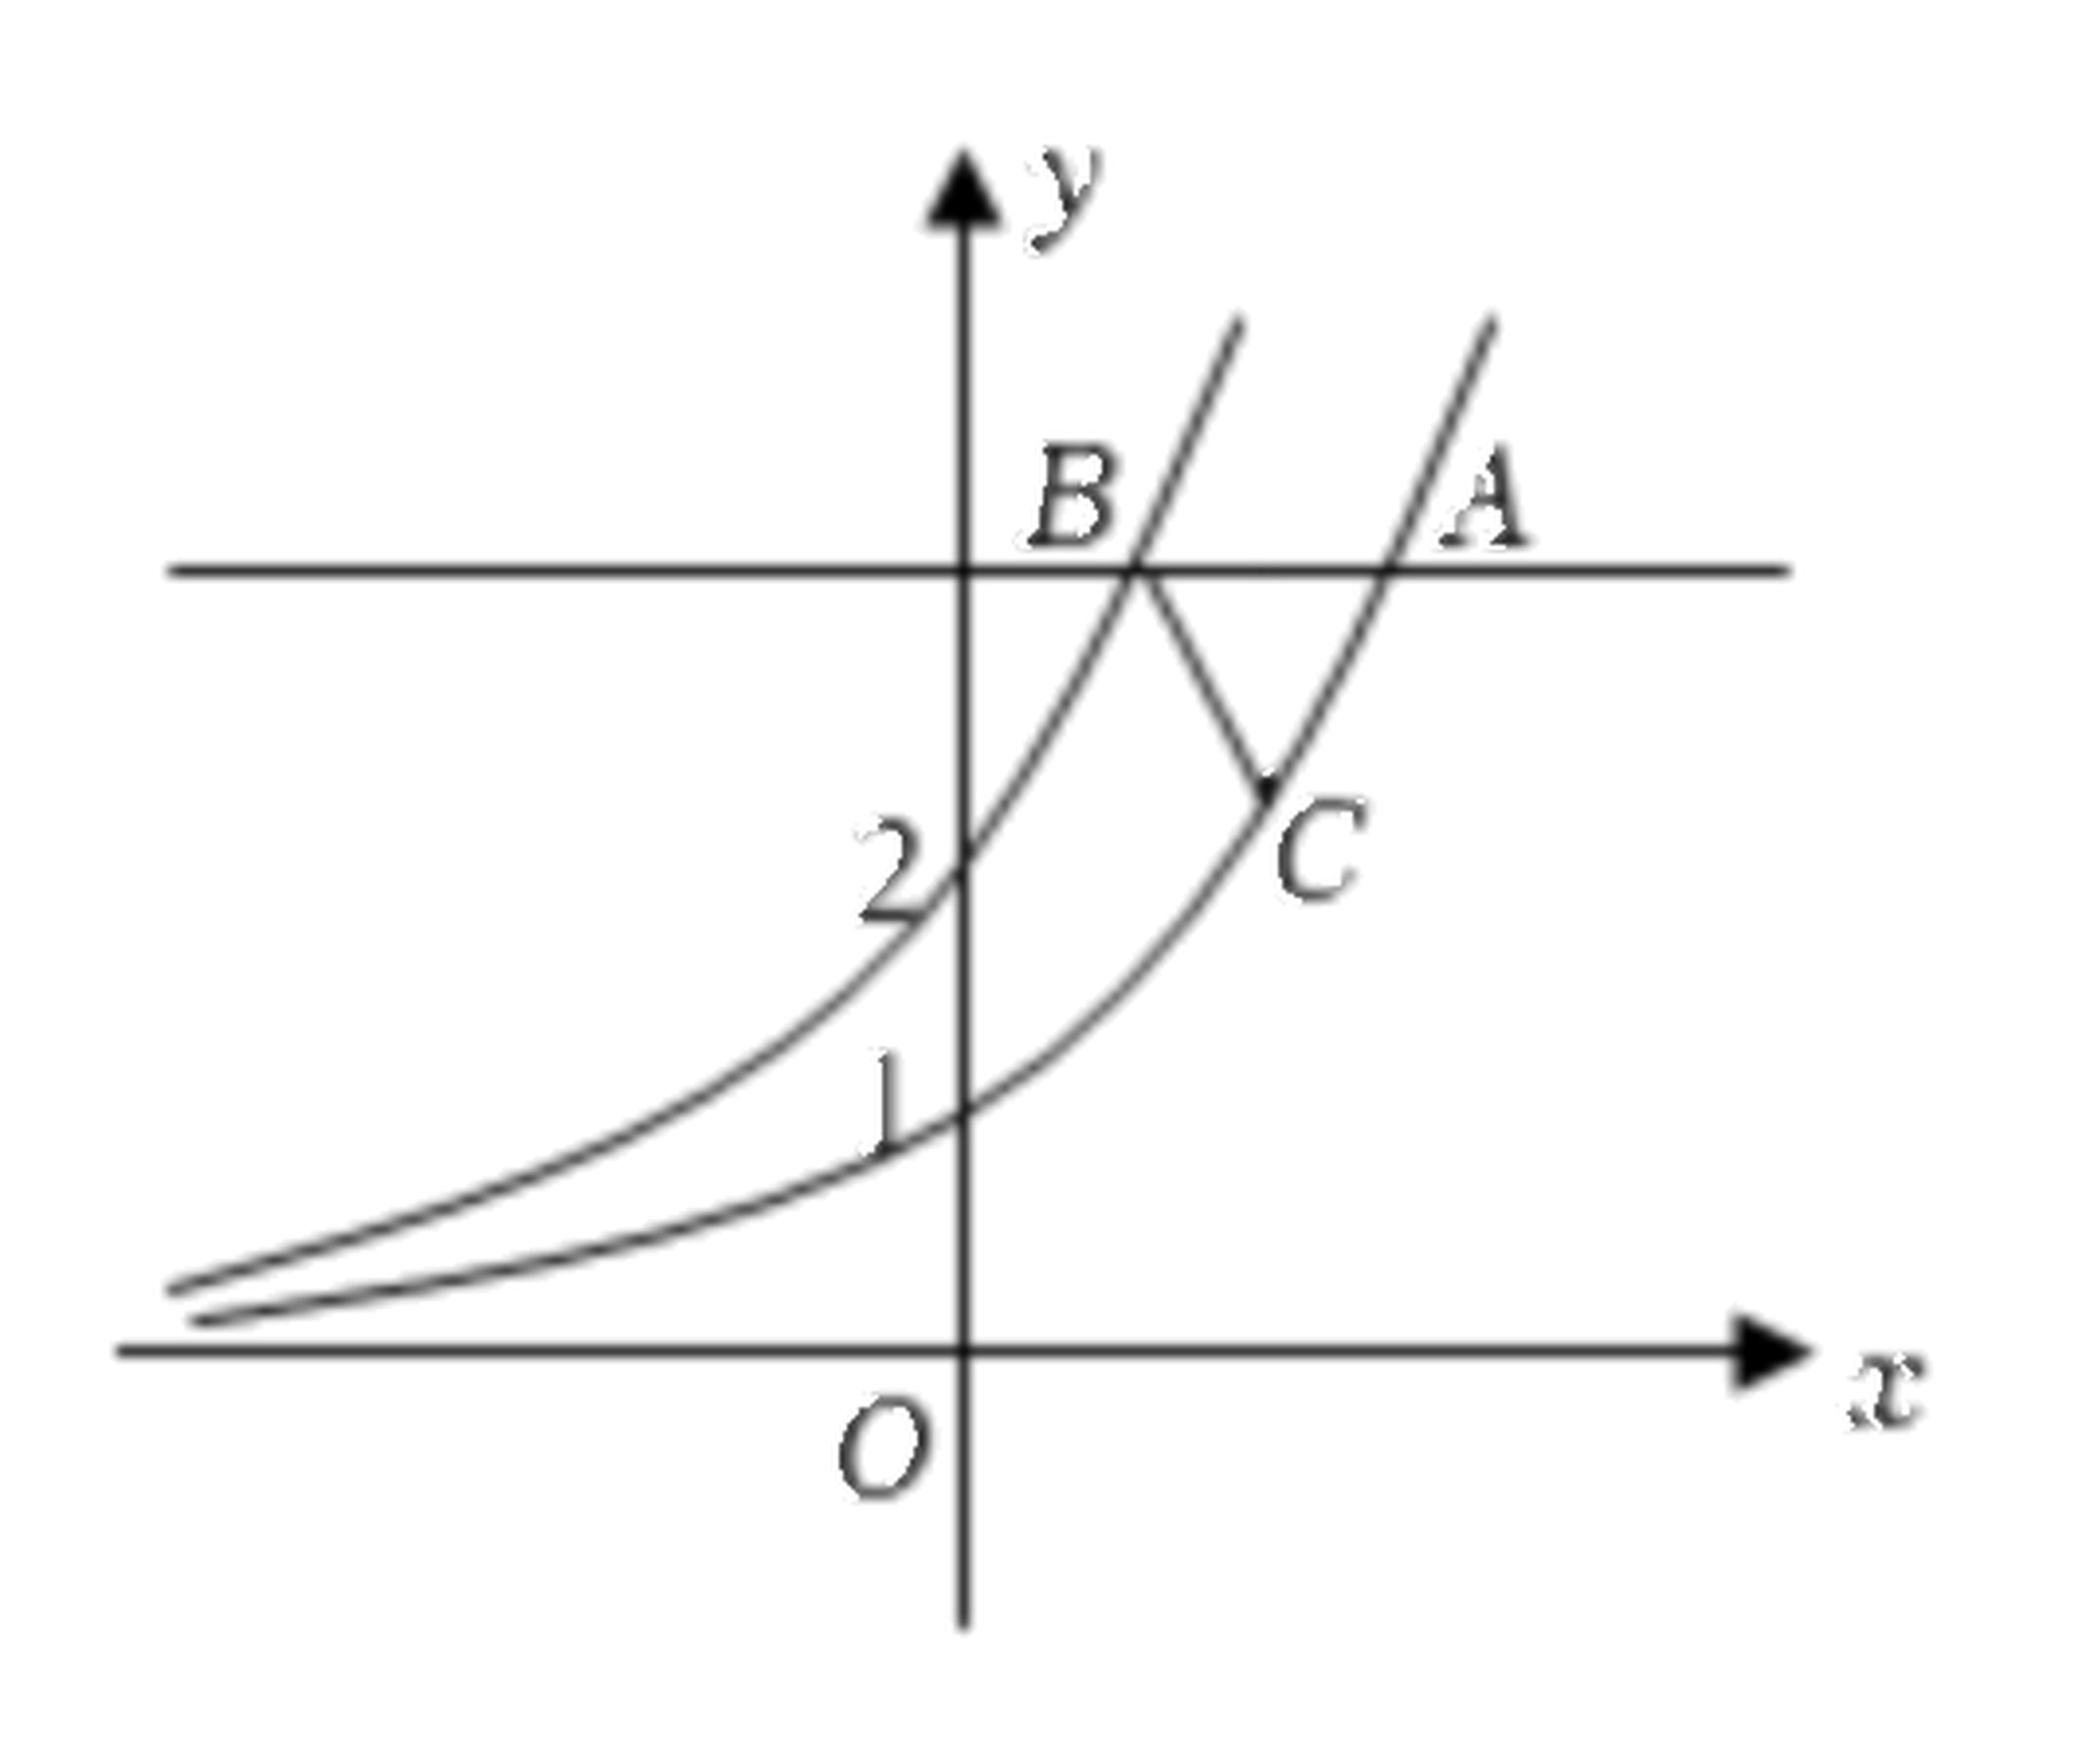
\includegraphics[width=0.40\textwidth]{figures/gao150_q11.png}
\end{center}

\ifanswer
\solbegin
\step{设直线 $l$ 的方程为 $y=a(a>0)$，}
\step{由 $2^x=a$，得 $x=\log_2 a$，所以 $A(\log_2 a,a)$，}
\step{由 $2^{x+1}=a$，得 $x=\log_2 a-1$，所以 $B(\log_2 a-1,a)$，所以 $\lvert AB\rvert=1$，}
\step{取 $AB$ 的中点 $D$，连接 $CD$，如图所示，}
\step{因为 $\triangle ABC$ 为等边三角形，则 $CD\perp AB$，且 $\lvert CD\rvert=\dfrac{\sqrt3}{2}$，}
\step{所以 $C\left(\log_2 a-\dfrac{1}{2},a-\dfrac{\sqrt3}{2}\right)$，}
\step{因为点 $C$ 在函数 $y=2^x$ 的图像上，所以 $a-\dfrac{\sqrt3}{2}=2^{\log_2 a-\frac{1}{2}}=\dfrac{a}{\sqrt2}$，}
\step{解得 $a=\dfrac{\sqrt3}{2-\sqrt2}=\dfrac{\sqrt3(2+\sqrt2)}{4-2}=\sqrt3+\dfrac{\sqrt6}{2}$，}
\step{所以点 $C$ 的纵坐标为 $a-\dfrac{\sqrt3}{2}=\dfrac{\sqrt3+\sqrt6}{2}$.}
\solend
\fi

% === Q12 === 解析配图（高斯函数方格阴影，仅答案版出）；"数学王子"弯引号；cases 块整体算一个印刷行；解析 4 行
\item 小玲在研究数学发展史，特别崇拜近代数学奠基者之一、享有“数学王子”称号的德国数学家高斯. 为了纪念高斯，我们把取整函数 $y=[x]$ 称为高斯函数，其中 $[x]$ 表示不超过 $x$ 的最大整数，如 $[1.1]=1$，$[-1.1]=-2$，则点集 $P=\{(x,y)\mid [x]^2+[y]^2=1\}$ 所表示的平面区域的面积为\blankline[4.4em].

\ifanswer
\solbegin
\step{$[x]^2+[y]^2=1$ 由 $\begin{cases}[x]=0\\ {[y]=-1}\end{cases}$ 或 $\begin{cases}[x]=0\\ {[y]=1}\end{cases}$ 或 $\begin{cases}[x]=-1\\ {[y]=0}\end{cases}$ 或 $\begin{cases}[x]=1\\ {[y]=0}\end{cases}$ 四个平面区域组成，}
\step{即 $\begin{cases}0\leqslant x<1\\ -1\leqslant y<0\end{cases}$ 或 $\begin{cases}0\leqslant x<1\\ 1\leqslant y<2\end{cases}$ 或 $\begin{cases}-1\leqslant x<0\\ 0\leqslant y<1\end{cases}$ 或 $\begin{cases}1\leqslant x<2\\ 0\leqslant y<1\end{cases}$，}
\step{作出平面区域如图所示，平面区域由四个边长为 $1$ 的正方形组成，}
\begin{center}
% 高斯函数 [x]^2+[y]^2=1 方格阴影区域图取 04 页顶部，去粉色水印、去色、4× LANCZOS 放大；仅答案版出
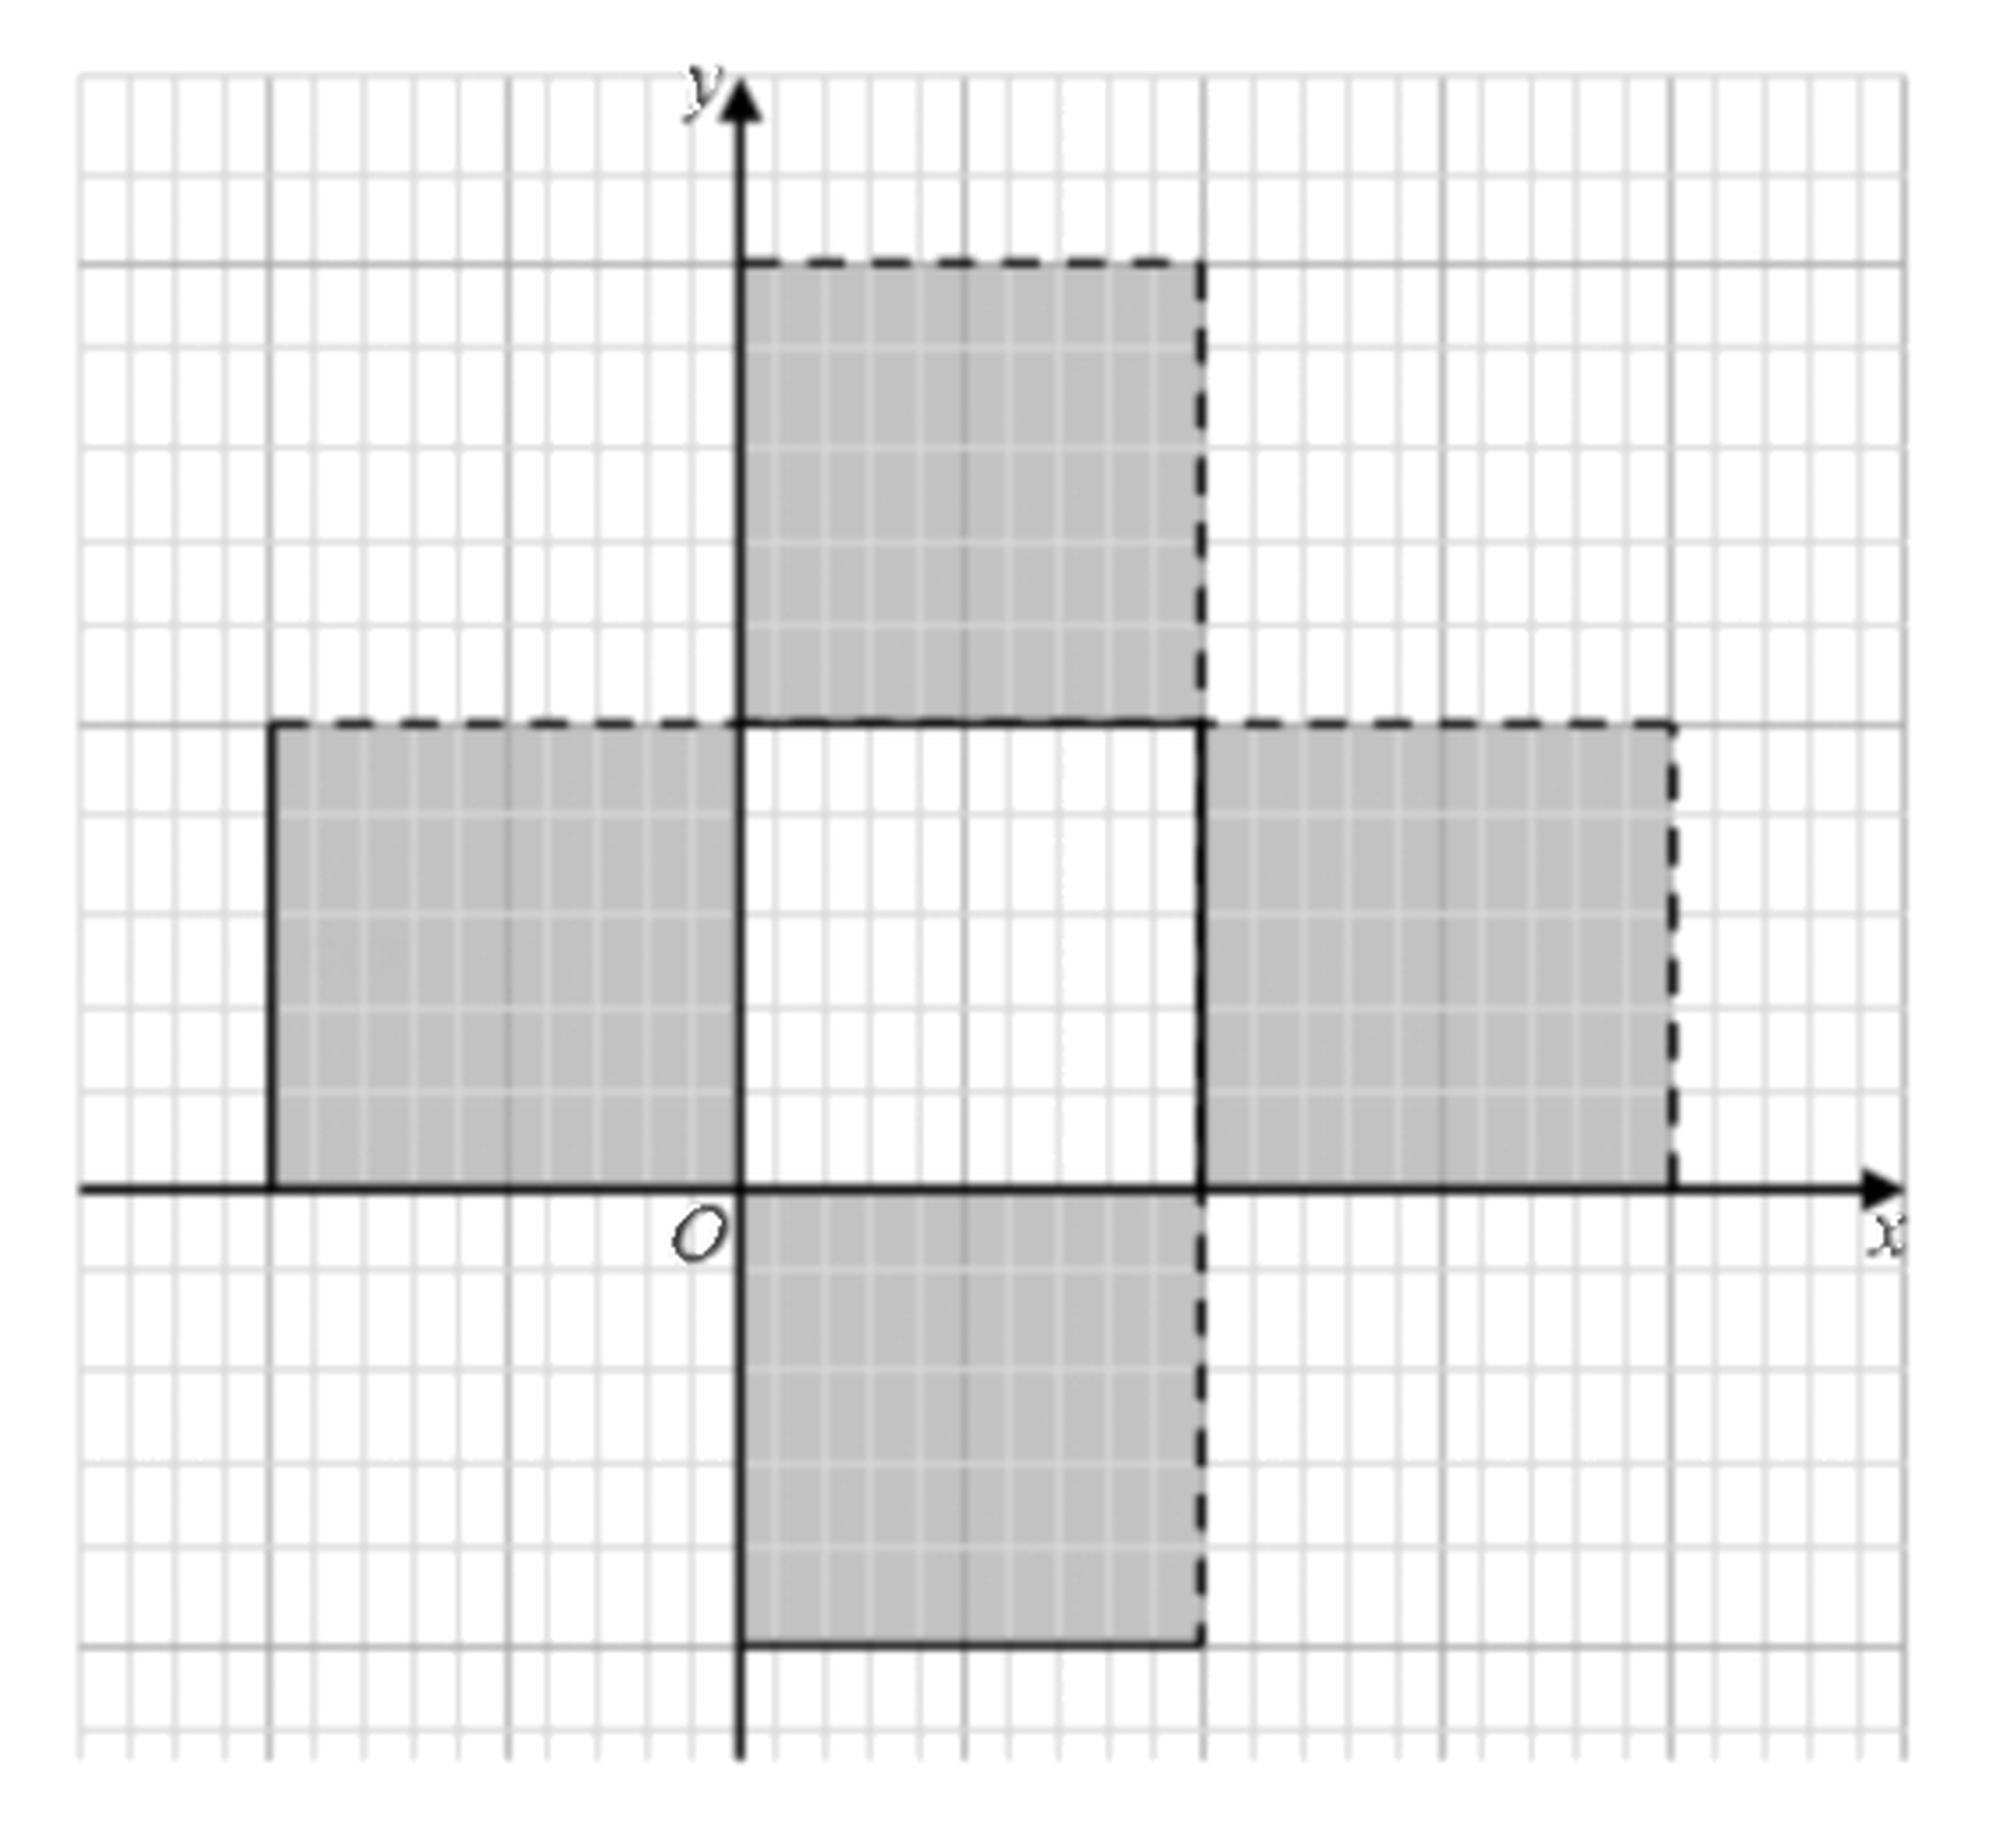
\includegraphics[width=0.34\textwidth]{figures/gao150_q12.png}
\end{center}
\step{总面积为 $1\times4=4$.}
\solend
\fi

\end{enumerate}

\bigsec{二、选择题}

\begin{enumerate}
\setcounter{enumi}{12}

% === Q13 === 答案在解析末句"故选 C"；括号 \mbox{（\quad）} 留空；四选项一行；解析 1 行
\item 设 $x\ne0$，则 $3^{\log_9 x^2}$ 的化简结果是\mbox{（\quad）}

\keepwithprev
A. $x$\qquad B. $\dfrac{1}{x}$\qquad C. $\lvert x\rvert$\qquad D. $\dfrac{1}{\lvert x\rvert}$

\ifanswer
\solbegin
\step{$3^{\log_9 x^2}=3^{\log_3\lvert x\rvert}=\lvert x\rvert$，故选 $C$.}
\solend
\fi

% === Q14 === 题目配图（两函数图像，三版都出）；\needvspace{8cm} 守卫放 \item 之前；"图像"照录；四选项两行两列；解析 2 行，故选 B
\needvspace{8cm}
\item 设 $a>0$ 且 $a\ne1$，$b\in\R$. 若函数 $y=a^{-\lvert x\rvert}$ 与 $y=x^b$ 的大致图像如图所示，则\mbox{（\quad）}

\keepwithprev
A. $0<a<1<b$\qquad\qquad B. $a>1$ 且 $b>1$

C. $0<a<1$ 且 $0<b<1$\qquad\qquad D. $0<b<1<a$

\begin{center}
% 两函数 y=a^{-|x|} 与 y=x^b 大致图像取 04 页右侧，去粉色水印、去色、4× LANCZOS 放大；三版都出
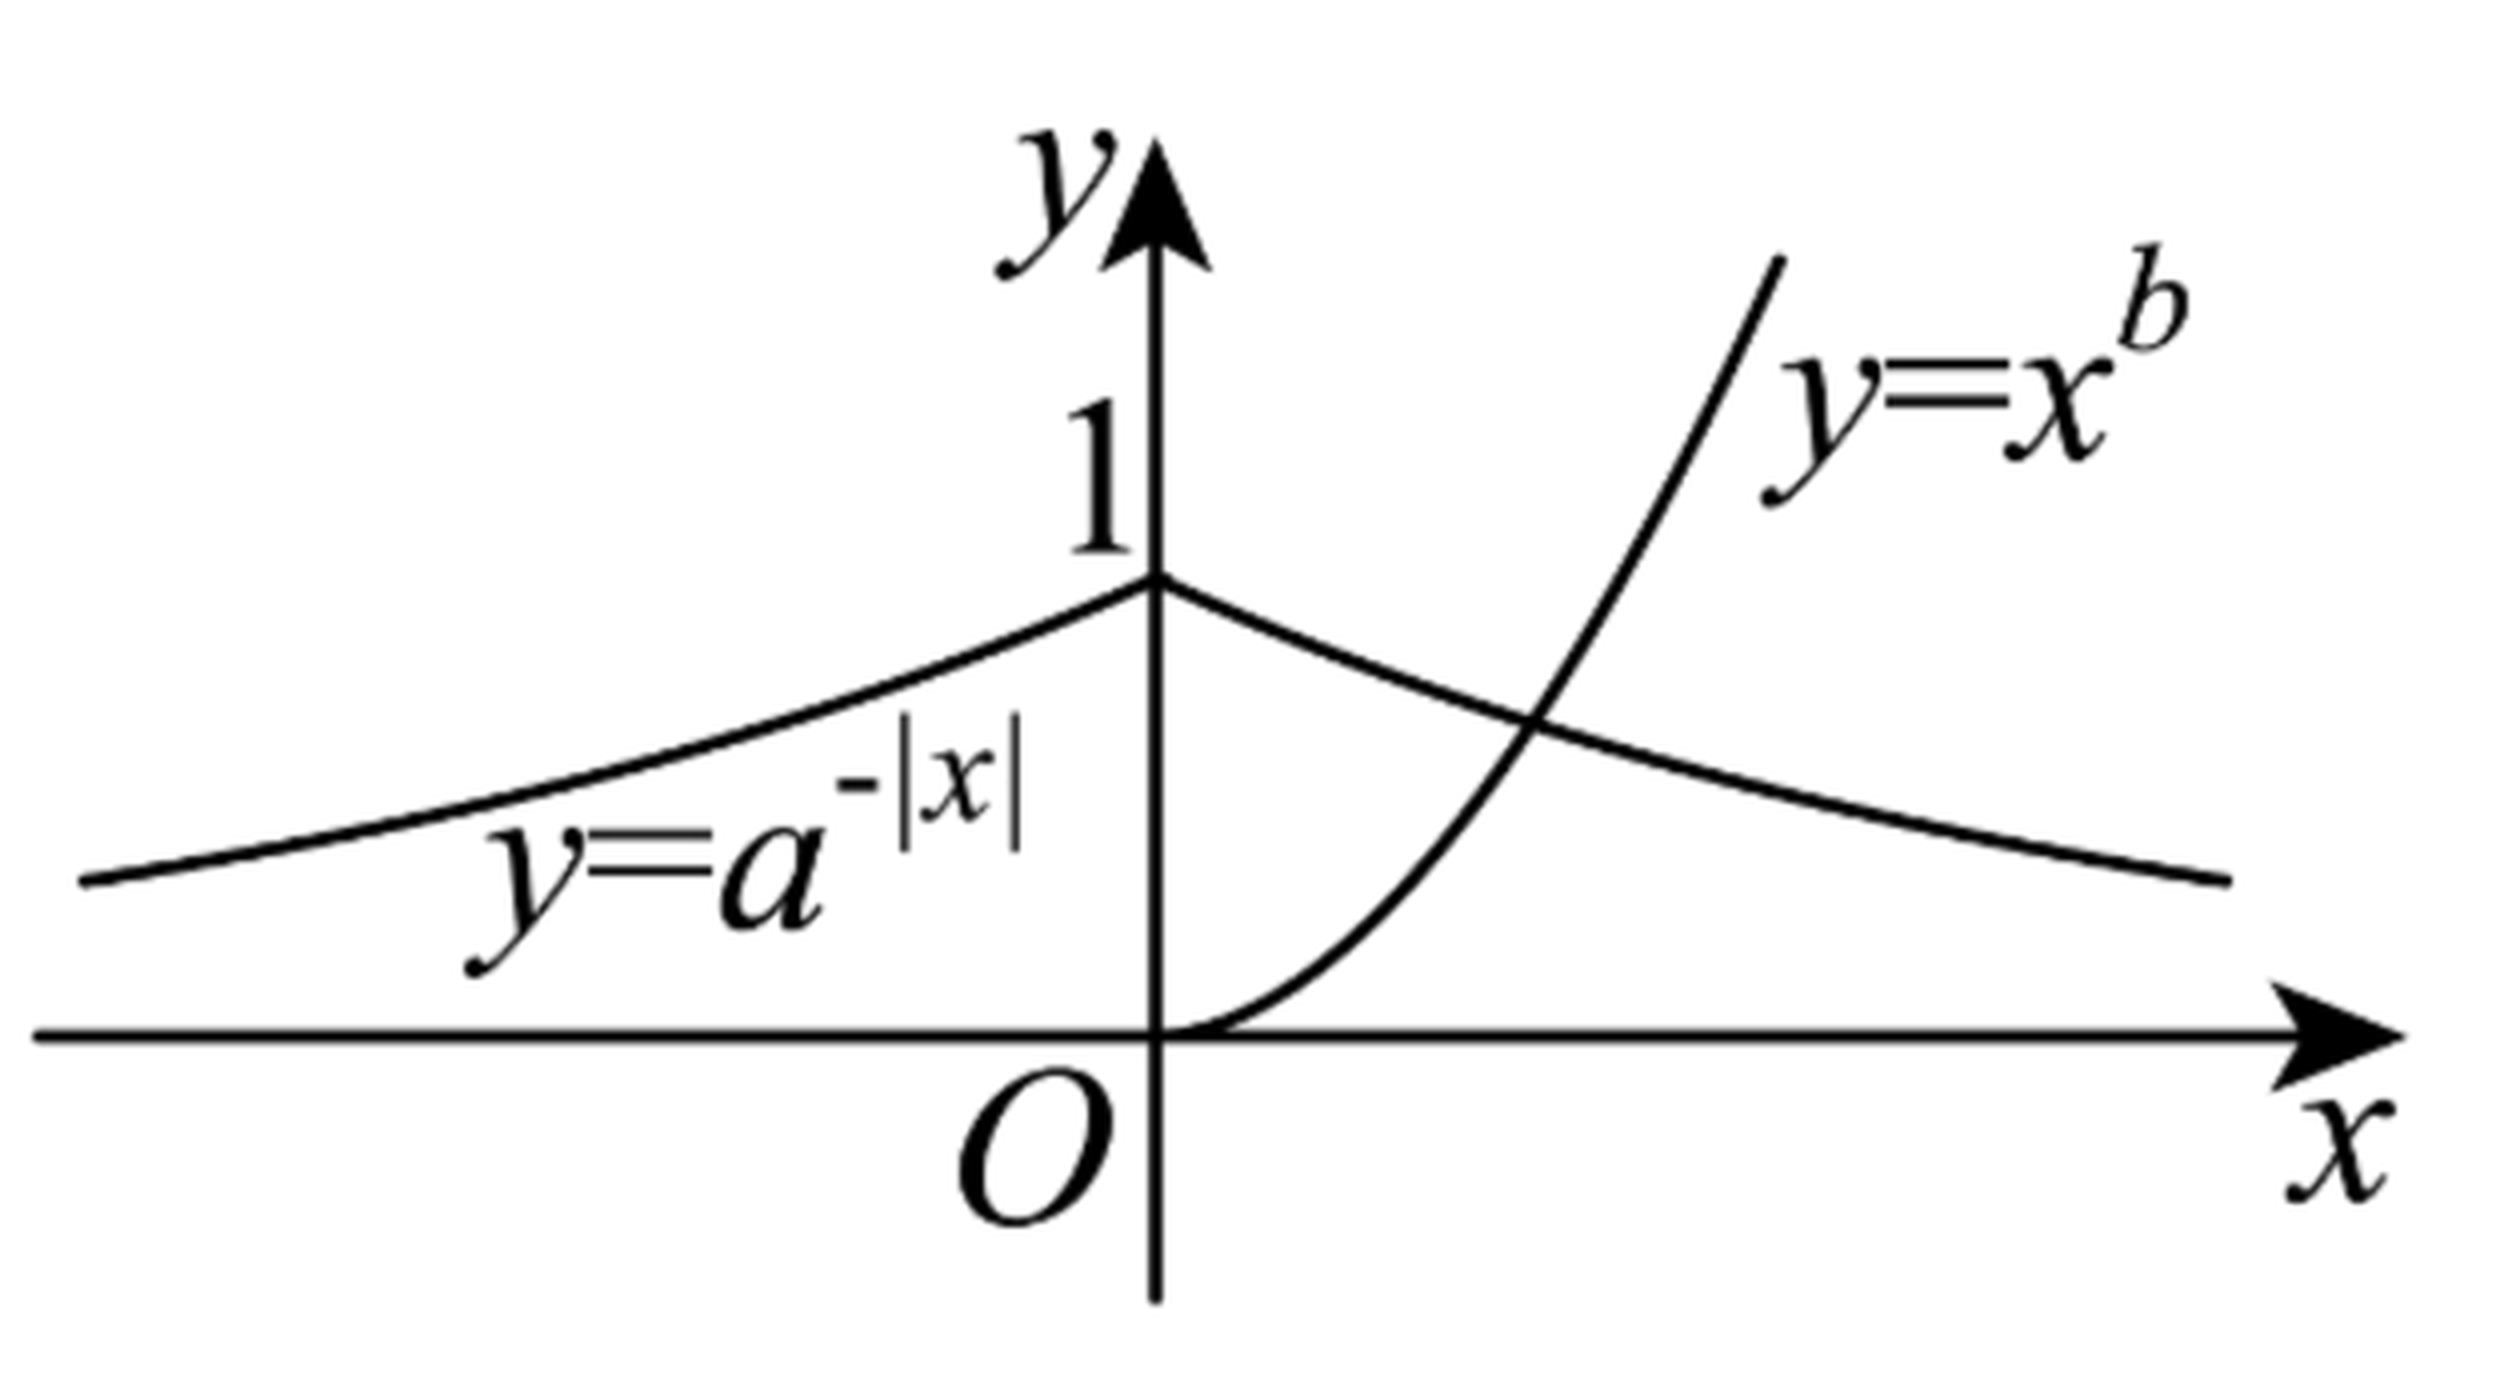
\includegraphics[width=0.40\textwidth]{figures/gao150_q14.png}
\end{center}

\ifanswer
\solbegin
\step{在 $(0,+\infty)$ 上，$y=a^{-x}$ 严格递减，得 $a>1$；}
\step{幂函数 $y=x^b$ 的图像递增且向上弯曲，得 $b>1$；故选 $B$.}
\solend
\fi

% === Q15 === "算术平均值／算术平均数"两处不同照录；四选项两行两列；解析 5 行（续 05 页顶），故选 B
\item 已知两个正数的算术平均值不小于它们的几何平均值，类比有以下结论：三个正数的算术平均数不小于它们的几何平均数，即当 $a,b,c$ 为正实数时，$\dfrac{a+b+c}{3}\geqslant\sqrt[3]{abc}$，当且仅当 $a=b=c$ 时等号成立. 利用上述结论，下列选项中判断正确的是\mbox{（\quad）}

\keepwithprev
A. 若 $x>0$，则 $2x+\dfrac{1}{x^2}\geqslant\dfrac{27}{8}$\qquad\qquad B. 若 $x>0$，则 $x^2+\dfrac{2}{x}\geqslant3$

C. 若 $0<x<1$，则 $x^2(1-x)\geqslant\dfrac{1}{9}$\qquad\qquad D. 若 $0<x<1$，则 $x^2(1-x)\leqslant\dfrac{1}{9}$

\ifanswer
\solbegin
\step{A：取 $x=1$，$2x+\dfrac{1}{x^2}=3<\dfrac{27}{8}$，错误.}
\step{B：$x^2+\dfrac{2}{x}=x^2+\dfrac{1}{x}+\dfrac{1}{x}\geqslant3\sqrt[3]{x^2\cdot\dfrac{1}{x}\cdot\dfrac{1}{x}}=3$，当且仅当 $x=1$ 时取等号，正确.}
\step{C：取 $x=\dfrac{1}{3}$，$x^2(1-x)=\dfrac{2}{27}<\dfrac{1}{9}$，错误.}
\step{D：取 $x=\dfrac{2}{3}$，$x^2(1-x)=\dfrac{4}{27}>\dfrac{1}{9}$，错误.}
\step{故选 $B$.}
\solend
\fi

% === Q16 === "完美集"新定义（弯引号、引号外空格照录）；圈数字①②文本模式；$n\in\N$；四选项两行两列；解析 9 行（6 行 05 页＋3 行 06 页顶），故选 A
\item 已知有限集 $A=\{a_1,a_2,\cdots,a_n\}$（$n\geqslant2$，$n\in\N$）. 若 $A$ 中元素 $a_i$（$i=1,2,\cdots,n$）满足 $a_1+a_2+\cdots+a_n=a_1\cdot a_2\cdots a_n$，就称 $A$ 为 “完美集”. 现有以下两个命题：

①恰有两个元素的 “完美集” 有无穷多个；

②若 $a_i$ 均为正整数，则 “完美集” $A$ 有且只有一个，且 $n=3$.

则\mbox{（\quad）}

\keepwithprev
A. ①和②都是真命题\qquad\qquad B. ①和②都是假命题

C. ①是真命题，②是假命题\qquad\qquad D. ①是假命题，②是真命题

\ifanswer
\solbegin
\step{①由 $a+b=ab\Leftrightarrow(a-1)(b-1)=1$，任取 $a>2$，则 $b=1+\dfrac{1}{a-1}\in(1,2)$，}
\step{得到无穷多个不同的完美集，①真.}
\step{②设 $1\leqslant a_1<a_2<\cdots<a_n$，则 $a_i\geqslant i$.}
\step{若 $n=2$，则 $(a_1-1)(a_2-1)=1$，只能有 $a_1=a_2=2$，与元素互异矛盾.}
\step{若 $n\geqslant4$，则 $a_1a_2\cdots a_n\geqslant a_2a_{n-1}a_n\geqslant2(n-1)a_n>na_n\geqslant a_1+\cdots+a_n$，矛盾.}
\step{当 $n=3$ 时，若 $a_1\geqslant2$，则 $a_1a_2a_3\geqslant6a_3>3a_3\geqslant a_1+a_2+a_3$，矛盾.}
\step{因此 $a_1=1$，$(a_2-1)(a_3-1)=2$，结合 $a_2<a_3$ 得 $a_2=2$，$a_3=3$.}
\step{唯一的完美集为 $\{1,2,3\}$，②真.}
\step{故选 $A$.}
\solend
\fi

\end{enumerate}

\bigsec{三、解答题}

\begin{enumerate}
\setcounter{enumi}{16}

% === Q17 === \varnothing 空集、$B\subseteq A$ 带下划线照录；弯引号内空格照录；解析 7 行
\item 设 $a,b\in\R$. 已知集合 $A=\{x\mid ax^2+3x-a>3\}$，$B=\{x\mid bx=1\}$.

(1) 若 $A=(1,2)$，求 $a$ 的值；

(2) 若 $a=0$，且 “ $x\in A$ ” 是 “ $x\in B$ ” 的必要非充分条件，求 $b$ 的取值范围.

\ifanswer
\solbegin
\step{(1) $A=(1,2)$，则 $a<0$，且 $1,2$ 是方程 $ax^2+3x-a-3=0$ 的两根.}
\step{由 $4a+6-a-3=0$，得 $a=-1$，此时不等式为 $-(x-1)(x-2)>0$，}
\step{解集确为 $(1,2)$.}
\step{(2) $a=0$ 时，$A=(1,+\infty)$，题意等价于 $B\subseteq A$ 且 $B\ne A$.}
\step{当 $b=0$ 时，$B=\varnothing$，符合条件.}
\step{当 $b\ne0$ 时，$B=\left\{\dfrac{1}{b}\right\}$，条件等价于 $\dfrac{1}{b}>1$，解得 $0<b<1$.}
\step{因此 $b$ 的取值范围为 $[0,1)$.}
\solend
\fi

% === Q18 === $p\in\Z$；"图像"（像，有亻）照录；指数 $-2p^2+5p$；解析 8 行（(1) 首行 06 页末＋2 行 07 页顶、(2) 5 行 07 页）
\item 设 $p\in\Z$，已知 $f(x)=x^{-2p^2+5p}$.

(1) 若幂函数 $y=f(x)$ 的图像关于原点成中心对称，且满足 $f(3)<f(4)$，求 $p$ 的值；

(2) 当 $p=-2$ 时，求满足 $f(2x+3)<f(x-4)$ 的 $x$ 的取值范围.

\ifanswer
\solbegin
\step{(1) 图像关于原点成中心对称，得整数 $-2p^2+5p$ 为奇数.}
\step{由 $f(3)<f(4)$，得 $-2p^2+5p>0\Leftrightarrow0<p<\dfrac{5}{2}$，}
\step{结合 $p\in\Z$，得 $p=1$ 或 $p=2$，对应指数分别为 $3$、$2$，所以 $p=1$.}
\step{(2) 当 $p=-2$ 时，$f(x)=\dfrac{1}{x^{18}}$，定义域为 $\{x\in\R\mid x\ne0\}$.}
\step{原不等式要求 $x\ne-\dfrac{3}{2}$ 且 $x\ne4$，}
\step{此时 $\dfrac{1}{(2x+3)^{18}}<\dfrac{1}{(x-4)^{18}}\Leftrightarrow\lvert 2x+3\rvert>\lvert x-4\rvert\Leftrightarrow(2x+3)^2>(x-4)^2$，}
\step{因此 $(x+7)(3x-1)>0\Leftrightarrow x<-7$ 或 $x>\dfrac{1}{3}$，}
\step{排除 $x=4$，得 $x\in(-\infty,-7)\cup\left(\dfrac{1}{3},4\right)\cup(4,+\infty)$.}
\solend
\fi

% === Q19 === $a\in\R$、$g(x)=f(2x+1)+a\cdot f(x)+2$；解析 6 行（(2) 末两行续 08 页顶）
\item 已知 $f(x)=2^x$.

(1) 求方程 $f(2x)-f(x)=6$ 的解；

(2) 设 $a\in\R$，$g(x)=f(2x+1)+a\cdot f(x)+2$，若对于任意 $x\in[-1,1]$，均有 $g(x)\geqslant1$，求 $a$ 的取值范围.

\ifanswer
\solbegin
\step{(1) 令 $t=2^x>0$，则 $t^2-t-6=(t-3)(t+2)=0$，}
\step{由 $t>0$ 得 $t=3$，所以 $x=\log_2 3$.}
\step{(2) 令 $t=2^x$，则 $t\in\left[\dfrac{1}{2},2\right]$，且 $g(x)\geqslant1\Leftrightarrow2t^2+at+1\geqslant0\Leftrightarrow a\geqslant-\left(2t+\dfrac{1}{t}\right)$，}
\step{由基本不等式得 $2t+\dfrac{1}{t}\geqslant2\sqrt{2t\cdot\dfrac{1}{t}}=2\sqrt2$，}
\step{当且仅当 $t=\dfrac{1}{\sqrt2}\in\left[\dfrac{1}{2},2\right]$ 时等号成立，}
\step{因此 $-\left(2t+\dfrac{1}{t}\right)$ 的最大值为 $-2\sqrt2$，所求范围为 $a\in[-2\sqrt2,+\infty)$.}
\solend
\fi

% === Q20 === "极闭集"新定义、3 问，全卷末题；$M\subseteq(0,+\infty)$ 带下划线照录；自定义运算 $x*y$ 星号照录；解析 13 行（9 行 08 页＋4 行 09 页上半）
\item 对于非空实数集 $M\subseteq(0,+\infty)$，若满足以下两个条件：

① $M$ 中至少含有 $2$ 个元素，且 $1\notin M$；

②对于 $M$ 中任意两个不相等的元素 $x$、$y$，定义 $x*y=\dfrac{xy+1}{x+y}$，且 $x*y\in M$.

则称 $M$ 为 “极闭集”.

(1) 分别判断集合 $A=\left\{\dfrac{1}{2},3\right\}$ 与集合 $B=(1,+\infty)$ 是否为 “极闭集” （无需理由）；

(2) 若 $M$ 是 “极闭集”，证明：$M$ 中不可能所有元素都小于 $1$；

(3) 证明：不存在任何有限集是 “极闭集”.

\ifanswer
\solbegin
\step{(1) $A$ 不是 “极闭集”，$B$ 是 “极闭集”.}
\step{(2) 假设 $M$ 中所有元素都小于 $1$，取其中两个不相等的元素 $x$、$y$，}
\step{则 $x*y-1=\dfrac{(1-x)(1-y)}{x+y}>0$，}
\step{这与 $x*y\in M$ 且 $M$ 中所有元素都小于 $1$ 矛盾.}
\step{(3) 假设有限集 $M$ 是 “极闭集”，}
\step{由 (2) 及 $1\notin M$，得 $M$ 中存在大于 $1$ 的元素.}
\step{若 $M$ 中有小于 $1$ 的元素，取其中最大的一个为 $a$，另取 $b\in M$ 且 $b>1$，}
\step{则 $a*b-a=\dfrac{1-a^2}{a+b}>0, a*b-1=\dfrac{(a-1)(b-1)}{a+b}<0$，}% 半角逗号在两个数学式组之间，全稿惯例、非笔误，照录
\step{于是 $a<a*b<1$ 且 $a*b\in M$，与 $a$ 的最大性矛盾.}
\step{若 $M$ 中没有小于 $1$ 的元素，则 $M\subseteq(1,+\infty)$.}
\step{取 $a=\min M$，另取 $b\in M$ 且 $b\ne a$，则 $a*b-a=\dfrac{1-a^2}{a+b}<0$，}
\step{于是 $a*b<a$ 且 $a*b\in M$，与 $a$ 的最小性矛盾.}
\step{因此不存在任何有限集是 “极闭集”.}
\solend
\fi

\end{enumerate}

\end{document}
"
%
% ① 原始材料：微信公众号"魔都数学加油站"文章，连载"27学年高一150"，原文标题
% "27学年高一150——2026-2027年上海市曹杨二中高一上期中"；
% 原文链接：https://mp.weixin.qq.com/s/xlQxmik8TZXR87RC6MnCrw 。
% 正文为 9 张 PNG 页（01/02/04/06/07/09 为 2560×3620，03/05/08 为 4762×6735，
% 同一篇各页分辨率混排，逐页按各自分辨率裁图核对，别按预览比例换算裁框）。
% 体例：讲评版——全 18 题均印【解析】（逐题核实，见 ② ②）。
% 题目、答案、解析均据原图转录；卷面粉红色/红色水印"魔都数学加油站"及公众号页脚未录入。
% 全卷插图清单（逐页通读 9 页确认）：3 幅——
%   · Q11 题目配图（指数函数曲线图，02 页右侧：x/y 轴、O、y=2^x 与 y=2^{x+1}
%     两曲线、A/B/C 三点、刻度 1/2、等边三角形 ABC），三版都出，裁 figures/gao150_q11.png；
%   · Q12 解析配图（高斯函数取整 [x]^2+[y]^2=1 方格阴影区域图，04 页顶部：4 个边长 1
%     的正方形组成的十字形阴影），解析"作出平面区域如图所示"处，仅答案版出，
%     放 \ifanswer 内 \step 之间，裁 figures/gao150_q12.png；
%   · Q14 题目配图（两函数 y=a^{-|x|} 与 y=x^b 大致图像，04 页右侧：x/y 轴、O、
%     y 轴刻度 1、一递减曲线一递增上翘曲线），三版都出，裁 figures/gao150_q14.png；
%   其余各页逐页确认无其它题目配图、无表格；Q11/Q12 解析"如图所示"对应的就是上列
%   已裁的图，不重复裁；09 页上半为 Q20(3) 解析续尾、下半仅水印、无正文。
%   3 图均取自原卷截图，去粉色水印、去色、4× LANCZOS 放大。
%
% 卷首标题：原卷印作"2026-2027 年曹杨二中高一上期中"，年份区间按全稿惯例排 en dash；
% 原卷卷面未印副标题，本稿按同期中卷知识模块口径补出"集合与常用逻辑用语、不等式、函数"。
%
% 题号体例（逐页核实定稿）：本卷共 18 题——一、填空题 3—12（10 题）、
% 二、选择题 13—16（4 题）、三、解答题 17—20（4 题）。
% 三节分别 \setcounter{enumi}{2}／{12}／{16}。原卷从第 3 题起、无第 1、2 题，
% 本稿保留原题号；全卷末题为第 20 题（"极闭集"新定义、3 问），无 Q21、无附加题节。
%
% ② 与原卷的排版差异：
%   ① 原文从第 3 题起，本稿保留原题号；共 18 题三节，解答题只有 4 题到 20；
%   ② 全 18 题均印【解析】，用 \solbegin…\solend；逐题核实无只印【答案】或
%      答案印题干括号内的题；四道选择题答案在解析末句"故选 X"（Q13 选 C、
%      Q14 选 B、Q15 选 B、Q16 选 A，逐个放大复核）、括号 \mbox{（\quad）} 留空、
%      不另提 \ans{}；答案版【答案】/【解析】标记数 = 18 = 全卷题数；
%   ③ 原卷卷面未印副标题，本稿按知识模块口径补出；
%   ④ 原卷填空横线按全稿惯例排 \blankline[4.4em]；选择题括号排 \mbox{（\quad）}、
%      选项段前按惯例加 \keepwithprev；解答题不留作答区、不加 \anspace（原卷为讲评版）；
%   ⑤ 数集黑板粗体：Q4"m\in R"、Q5"a,b\in R"、Q6"a,b,c\in R"、Q7"a\in R"、
%      Q10"a\in R"、Q14"b\in R"、Q17"a,b\in R"、Q18"p\in Z"／定义域"x\in R"、
%      Q19"a\in R"、Q16"n\in N" 原卷印斜体 R/Z/N，按全稿惯例归一 \R／\Z／\N；
%      绝对值排 \lvert…\rvert（Q7 |x+4|+|x-3|、Q11 |AB|／|CD|、Q13 |x|、
%      Q18 |2x+3|／|x-4|），集合描述竖线排 \mid（Q3、Q12、Q17、Q18、Q20），
%      不等号按全稿惯例排 \leqslant／\geqslant；补集照原卷上划线排 \overline{A}
%      （Q3 题干＋解析共 2 处）；空集符号 \varnothing（Q17 解析(2)）；
%      子集 \subset（单线⊂）／\subseteq（带下划线⊆）逐处照录，本卷 3 处子集
%      符号均印带下划线 ⊆、照录 \subseteq（Q20 题干、Q20 解析(3)、Q17 解析(2)，
%      见 ④），无 \subset 用例；
%   ⑥ 判别式 Δ/△：逐页通读 9 页，本卷无一元二次判别式算式，故无 Δ/△ 混用可照录
%      （"高 \Delta／扁 \triangle"口径备查，参照 高一142／144／145／146／148／149
%      头注④）；本卷仅 Q11 题干与解析共 2 处几何三角形符号 △ABC，逐处放大并排
%      确认两处同形、印近等边粗线三角（非判别式），照录 \triangle（见 ④）；
%   ⑦ 中文弯引号照录：Q12"数学王子"、Q16"完美集"（题干＋①②两命题，引号外
%      留空格）、Q17" x∈A "" x∈B "（引号内空格）、Q20"极闭集"（题干条件、
%      三问与解析，引号外留空格）；注释里一律 ASCII 引号；数学式内 CJK 用 \text{}
%      （Q3 集合描述"且"用 \text{ 且 }）；
%   ⑧ 半角逗号在数学组之间是全稿惯例、非笔误，逐处照录（Q17 解析"1,2 是方程…
%      两根"、Q20 解析(3)">0, a*b-1=…<0" 两式之间等）；行末西文句点 ASCII `.`；
%      行中全角逗号／顿号照录（Q12"之一、享有"、Q18 解析"3、2"、Q20"x、y"）；
%   ⑨ "图像／图象"逐处放大核：全卷 9 处均印"图像"（像，有亻）、未见"图象"——
%      Q4 题干 1、Q11 题干 2＋解析 1、Q14 题干 1＋解析 1、Q18 题干 1＋解析 1；
%      同卷"第二象限""象限"用"象"（无亻）。逐处照录未统一改动（放大 01/02/04/06
%      页 /tmp/gao150/z/p01_q4_tuxiang2.png、p04_q14_tuxiang2.png、
%      p02_q11_lines.png 确认）；子题标号 (1)(2)(3) 半角括号照录；圈数字①②
%      在文本模式（Q16 两命题与解析、Q20 两条件与三问及解析）按 common.sty
%      划入 CJK 字符类渲染，进数学式用 \text{①}；
%   ⑩ Q20 新定义 x*y=\dfrac{xy+1}{x+y} 的 * 是自定义运算（星号），照录；
%      \left…\right 不得拆到不同 $…$ 组（Q19"\left(2t+\frac1t\right)"、
%      Q20 题干"A=\left\{\frac12,3\right\}"等）；Q8 嵌套根号
%      \sqrt{\frac2x+\frac{16}{1-2x}}、Q9 对数连加 \log_2 A 等复杂式照录别简化；
%   ⑪ 一条 \step = 原卷解析的一个印刷行，cases 块整体算一个印刷行；别并折行、
%      别拆行。Q4 三行、Q8 五行、Q11 九行、Q12 四行（两行各含四个 cases 块）、
%      Q15 五行、Q16 九行、Q18 八行、Q20 十三行均按印刷行逐条断，不丢行；
%   ⑫ 配图：Q11／Q14 题目配图（三版都出）放 \item 内题干之后 \begin{center}，
%      大图块加 \needvspace{8cm} 守卫把整块推走（守卫放 \item 之前，见
%      高一145 Q14/Q20 成例与切页审计 B 类坑）；Q12 解析配图（仅答案版出）
%      放 \ifanswer 内 \solbegin…\solend 的 \step 之间（高一73 第16题成例）；
%   ⑬ 跨页续印按题合并：见 ⑥；
%   ⑭ 原卷解析内无红色"法一／法二"之类小标题，故本卷无 \stepm；红色水印
%      "魔都数学加油站"不录入；Q12 解析"作出平面区域如图所示"对应的图即
%      ① 所列 gao150_q12.png（04 页顶部），不重复裁；Q11 解析"如图所示"对应
%      题目配图 gao150_q11.png，不另裁。
%
% ③ 行数复核：一条 \step／\stepm = 原卷解析的一个印刷行，cases 块作一个印刷行计。
%   逐题数（主会话逐页核对定稿）：Q3：1；Q4：3；Q5：2；Q6：1；Q7：2；Q8：5；
%   Q9：1；Q10：3；Q11：9；Q12：4；Q13：1；Q14：2；Q15：5；Q16：9；
%   Q17：7；Q18：8；Q19：6；Q20：13。
%   合计 82 条 \step（本卷无 \stepm：解析内无红色"法一／法二"类小标题），
%   与原卷逐题印刷行相等。全卷 18 题均设 \solbegin…\solend，答案版
%   【答案】/【解析】标记数 = 18 = 全卷题数。
%
% ④ 判别式／三角形／子集符号结论（逐处放大原图照录、不得统一，主会话像素级复核）：
%   判别式：逐页通读 9 页，本卷无一元二次判别式 Δ/△ 算式（Q18 讨论幂函数指数
%     奇偶、不用判别式；Q9／Q19／Q20 亦无），头注 ② ⑥ 的"高 \Delta／扁 \triangle"
%     口径在本卷无对应处（参照 高一142／144／145／146／148／149 头注④，仅备查）。
%   几何三角形符号：Q11 题干"使得 △ABC 为等边三角形"（02 页末）与解析
%     "因为 △ABC 为等边三角形，则 CD⊥AB"（03 页）共 2 处，放大 02/03 页
%     /tmp/gao150/z/q11_tri_montage2.png 并排确认两处同形、印近等边粗线三角
%     （h/w≈0.98、非"高>宽"的判别式 \Delta），照录 \triangle（与 高一105
%     "使得 \triangle ABC 为等边三角形" 同短语成例、高一149 几何三角形照录
%     \triangle 口径一致），不引入 \Delta。
%   子集／补集：Q20 题干"$M\subseteq(0,+\infty)$"（08 页）、Q20 解析(3)
%     "则 $M\subseteq(1,+\infty)$"（09 页）、Q17 解析(2)"题意等价于 $B\subseteq A$
%     且 $B\ne A$"（06 页）共 3 处子集符号，逐处放大（/tmp/gao150/z/p08_q20_stem.png、
%     p09_q20_sub.png、p06_q17_sub.png）确认均印带下划线 ⊆，照录 \subseteq；
%     本卷未见单线 ⊂（\subset）之对应处。Q3 题干与解析共 2 处补集照原卷上划线
%     排 \overline{A}；Q17 解析(2) 空集印 ∅、照录 \varnothing（Q7"解集为空集"
%     为中文词、非符号，照录文字）；集合描述竖线 \mid；数集 \R／\Z／\N 归一见 ② ⑤。
%
% ⑤ 存疑照录（放大原图确认，照录未改、正文对应处另有 % 注）：
%   1. Q8 解析第 4 行"所以 $y=\frac1x+\frac{8}{1-2x}$ 的最小值为 18" —— 上文
%      并未定义 $y$，且题面求的是 $\sqrt{\frac2x+\frac{16}{1-2x}}$ 的最小值；
%      按上下文该行应为 $\frac1x+\frac{8}{1-2x}$ 的最小值为 18（$y$ 疑为原卷
%      衍字／笔误），放大 02 页 /tmp/gao150/z/p02_q8_y.png 确认，照录未改。
%   2. Q20 解析(3)"$a*b-a=\frac{1-a^2}{a+b}>0, a*b-1=\frac{(a-1)(b-1)}{a+b}<0$"
%      两式之间的逗号原卷印半角 ,（非全角），按全稿惯例"半角逗号在数学组之间"
%      照录未改（放大 08 页 /tmp/gao150/z/p08_q20_sol8.png 确认）。
%   3. Q15 题干"两个正数的算术平均值…几何平均值"与"三个正数的算术平均数…
%      几何平均数"两处"值／数"用字不同，逐处照录未统一（放大 04 页确认）。
%   4. "图像／图象"全卷 9 处均印"图像"（像，有亻）、未见"图象"，逐处放大核实
%      照录、未统一改动（见 ② ⑨）；本卷判别式 Δ/△ 无用例、几何三角形 2 处
%      照录 \triangle（见 ④）。
%   全卷除此 4 类外未发现其它笔误／自相矛盾处；18 题均印【解析】、无只印【答案】
%   或答案印题干括号内的题（见 ② ②）。
%
% ⑥ 跨页续印按题合并说明（逐页核实定稿）：Q3/4/5/6/7 题干＋解析在 01 页；
%   Q8 题干＋解析 5 行、Q9 题干＋解析 1 行在 02 页上半；Q10 题干＋解析 3 行
%   在 02 页下半；Q11 题干（前两行）＋配图在 02 页下半、题干续"三角形，则点 C
%   的纵坐标为___"与解析 9 行全在 03 页上半（解析"如图所示"对应题目配图）；
%   Q12 题干＋解析 4 行在 03 页下半，解析配图（方格阴影）续印在 04 页顶部；
%   "二、选择题"标题在 04 页中部；Q13 题干＋选项＋解析、Q14 题干＋选项＋
%   配图＋解析在 04 页；Q15 题干＋四选项在 04 页末、解析 5 行续 05 页上半；
%   Q16 题干＋①②两命题＋"则(  )"＋四选项＋解析前 6 行在 05 页、解析末 3 行
%   （"因此 a_1=1…②真""故选 A"）续 06 页顶部；"三、解答题"标题在 06 页；
%   Q17 题干(1)(2)＋解析(1) 3 行＋解析(2) 首行在 06 页、解析(2) 续 3 行
%   在 06 页下半；Q18 题干(1)(2)＋解析(1) 首行在 06 页末、解析(1) 续 2 行＋
%   解析(2) 5 行在 07 页上半；Q19 题干(1)(2)＋解析(1) 2 行＋解析(2) 前 2 行
%   在 07 页下半、解析(2) 末 2 行续 08 页顶部；Q20 题干（新定义＋①②两条件）
%   ＋三问＋解析(1)(2)(3) 前 9 行在 08 页、解析(3) 末 4 行续 09 页上半，
%   末行"因此不存在任何有限集是极闭集"为全卷收尾（09 页下半仅水印、无正文）。
%   本稿按题连排，不丢行、不并折行；全卷末题为第 20 题，无 Q21、无附加题节。
%
\documentclass[a4paper,11pt]{article}
\usepackage{common}

\begin{document}

\examtitlest[3]{2026--2027 年曹杨二中高一上期中}{集合与常用逻辑用语、不等式、函数}

\bigsec{一、填空题}

\begin{enumerate}
\setcounter{enumi}{2}

% === Q3 === 补集上划线 \overline{A}（题干＋解析各 1 处）；集合描述竖线 \mid、数学式内"且"用 \text{}；解析 1 行
\item 设全集 $U=\{1,2,3,4,5\}$，集合 $A=\{x\mid x^2-3x\leqslant0\text{ 且 }x\in U\}$，则 $\overline{A}=$\blankline[4.4em].

\ifanswer
\solbegin
\step{$x^2-3x\leqslant0\Leftrightarrow0\leqslant x\leqslant3$，所以 $A=\{1,2,3\}$，$\overline{A}=\{4,5\}$.}
\solend
\fi

% === Q4 === "图像"（像，有亻）逐处照录、同句"第二象限"用"象"（无亻）；解析 3 行
\item 设 $m\in\R$. 若幂函数 $y=(m^2-5m+1)x^{m+1}$ 的图像经过第二象限，则 $m=$\blankline[4.4em].

\ifanswer
\solbegin
\step{幂函数的系数为 1，故 $m^2-5m+1=1\Rightarrow m=0$ 或 $m=5$.}
\step{$m=0$ 时，$y=x$ 不经过第二象限；}
\step{$m=5$ 时，$y=x^6$ 经过第二象限，因此 $m=5$.}
\solend
\fi

% === Q5 === 解析 2 行
\item 设 $a,b\in\R$. 若 $a^2+\dfrac{b^2}{4}=1$，则 $ab$ 的最大值为\blankline[4.4em].

\ifanswer
\solbegin
\step{$1-ab=\left(a-\dfrac{b}{2}\right)^2\geqslant0$，即 $ab\leqslant1$；}
\step{当 $a=\dfrac{\sqrt2}{2}$，$b=\sqrt2$ 时取等号，最大值为 1.}
\solend
\fi

% === Q6 === 解析 1 行
\item 设 $a,b,c\in\R$. 若等式 $2x^2-3x-2=a(x-1)^2+b(x-1)+c$ 恒成立，则 $a-b+c=$\blankline[4.4em].

\ifanswer
\solbegin
\step{令 $x=0$，得 $a-b+c=-2$.}
\solend
\fi

% === Q7 === 绝对值 \lvert…\rvert；解析 2 行
\item 设 $a\in\R$. 若关于 $x$ 的不等式 $\lvert x+4\rvert+\lvert x-3\rvert<a$ 的解集为空集，则 $a$ 的取值范围是\blankline[4.4em].

\ifanswer
\solbegin
\step{$\lvert x+4\rvert+\lvert x-3\rvert\geqslant\lvert(x+4)-(x-3)\rvert=7$，当 $-4\leqslant x\leqslant3$ 时取等号.}
\step{原不等式的解集为空集当且仅当 $a\leqslant7$，即 $a\in(-\infty,7]$.}
\solend
\fi

% === Q8 === 嵌套根号 \sqrt{\frac{2}{x}+\frac{16}{1-2x}} 照录别简化；解析 5 行
\item 设 $x\in\left(0,\dfrac{1}{2}\right)$，则 $\sqrt{\dfrac{2}{x}+\dfrac{16}{1-2x}}$ 的最小值为\blankline[4.4em].

\ifanswer
\solbegin
\step{因为 $x\in\left(0,\dfrac{1}{2}\right)$，所以 $1-2x>0$，又 $2x+1-2x=1$，}
\step{所以 $\left(\dfrac{1}{x}+\dfrac{8}{1-2x}\right)(2x+1-2x)=10+\dfrac{1-2x}{x}+\dfrac{16x}{1-2x}$}
\step{$\geqslant10+2\sqrt{\dfrac{1-2x}{x}\cdot\dfrac{16x}{1-2x}}=18$，}
\step{当且仅当 $\dfrac{1-2x}{x}=\dfrac{16x}{1-2x}$ 即 $x=\dfrac{1}{6}$ 时取等号，所以 $y=\dfrac{1}{x}+\dfrac{8}{1-2x}$ 的最小值为 18，}% 原卷此处径写 $y=\frac1x+\frac{8}{1-2x}$（上文未定义 $y$、且与题面根式不符），疑笔误，放大 02 页确认，照录未改（见 ⑤）
\step{所以 $\sqrt{\dfrac{2}{x}+\dfrac{16}{1-2x}}$ 的最小值为 6.}
\solend
\fi

% === Q9 === 对数连加 \log_2 A 等复杂式照录别简化；解析 1 行
\item 记 $A=1\times2\times3\times\cdots\times2026$，则 $\dfrac{1}{\log_2 A}+\dfrac{1}{\log_3 A}+\dfrac{1}{\log_4 A}+\cdots+\dfrac{1}{\log_{2026}A}=$\blankline[4.4em].

\ifanswer
\solbegin
\step{原式 $=\log_A 2+\cdots+\log_A 2026=\log_A(2\times3\times\cdots\times2026)=\log_A A=1$.}
\solend
\fi

% === Q10 === "严格减函数／不恒为负／⇔"照录；解析 3 行
\item 设 $a\in\R$，$f(x)=\dfrac{ax+1}{x+2}$. 若函数 $y=f(x)$ 在 $[1,+\infty)$ 上是严格减函数，且在 $[1,+\infty)$ 上的函数值不恒为负，则 $a$ 的取值范围是\blankline[4.4em].

\ifanswer
\solbegin
\step{当 $1\leqslant x_1<x_2$ 时，$f(x_2)-f(x_1)=\dfrac{(2a-1)(x_2-x_1)}{(x_1+2)(x_2+2)}$，故严格递减 $\Leftrightarrow a<\dfrac{1}{2}$.}
\step{此时最大函数值为 $f(1)$，函数值不恒为负 $\Leftrightarrow f(1)=\dfrac{a+1}{3}\geqslant0\Leftrightarrow a\geqslant-1$，}
\step{得 $a\in\left[-1,\dfrac{1}{2}\right)$.}
\solend
\fi

% === Q11 === 题目配图（指数函数曲线，三版都出）；\needvspace{8cm} 守卫放 \item 之前；"图像"照录、几何三角形 \triangle；解析 9 行（全在 03 页）
\needvspace{8cm}
\item 如图，点 $C$ 是函数 $y=2^x$ 的图像上的一点，若存在平行于 $x$ 轴的直线 $l$ 分别与函数 $y=2^x$ 和 $y=2^{x+1}$ 的图像相交于点 $A$、$B$，使得 $\triangle ABC$ 为等边三角形，则点 $C$ 的纵坐标为\blankline[4.4em].

\begin{center}
% 指数函数曲线图取 02 页右侧，去粉色水印、去色、4× LANCZOS 放大；三版都出
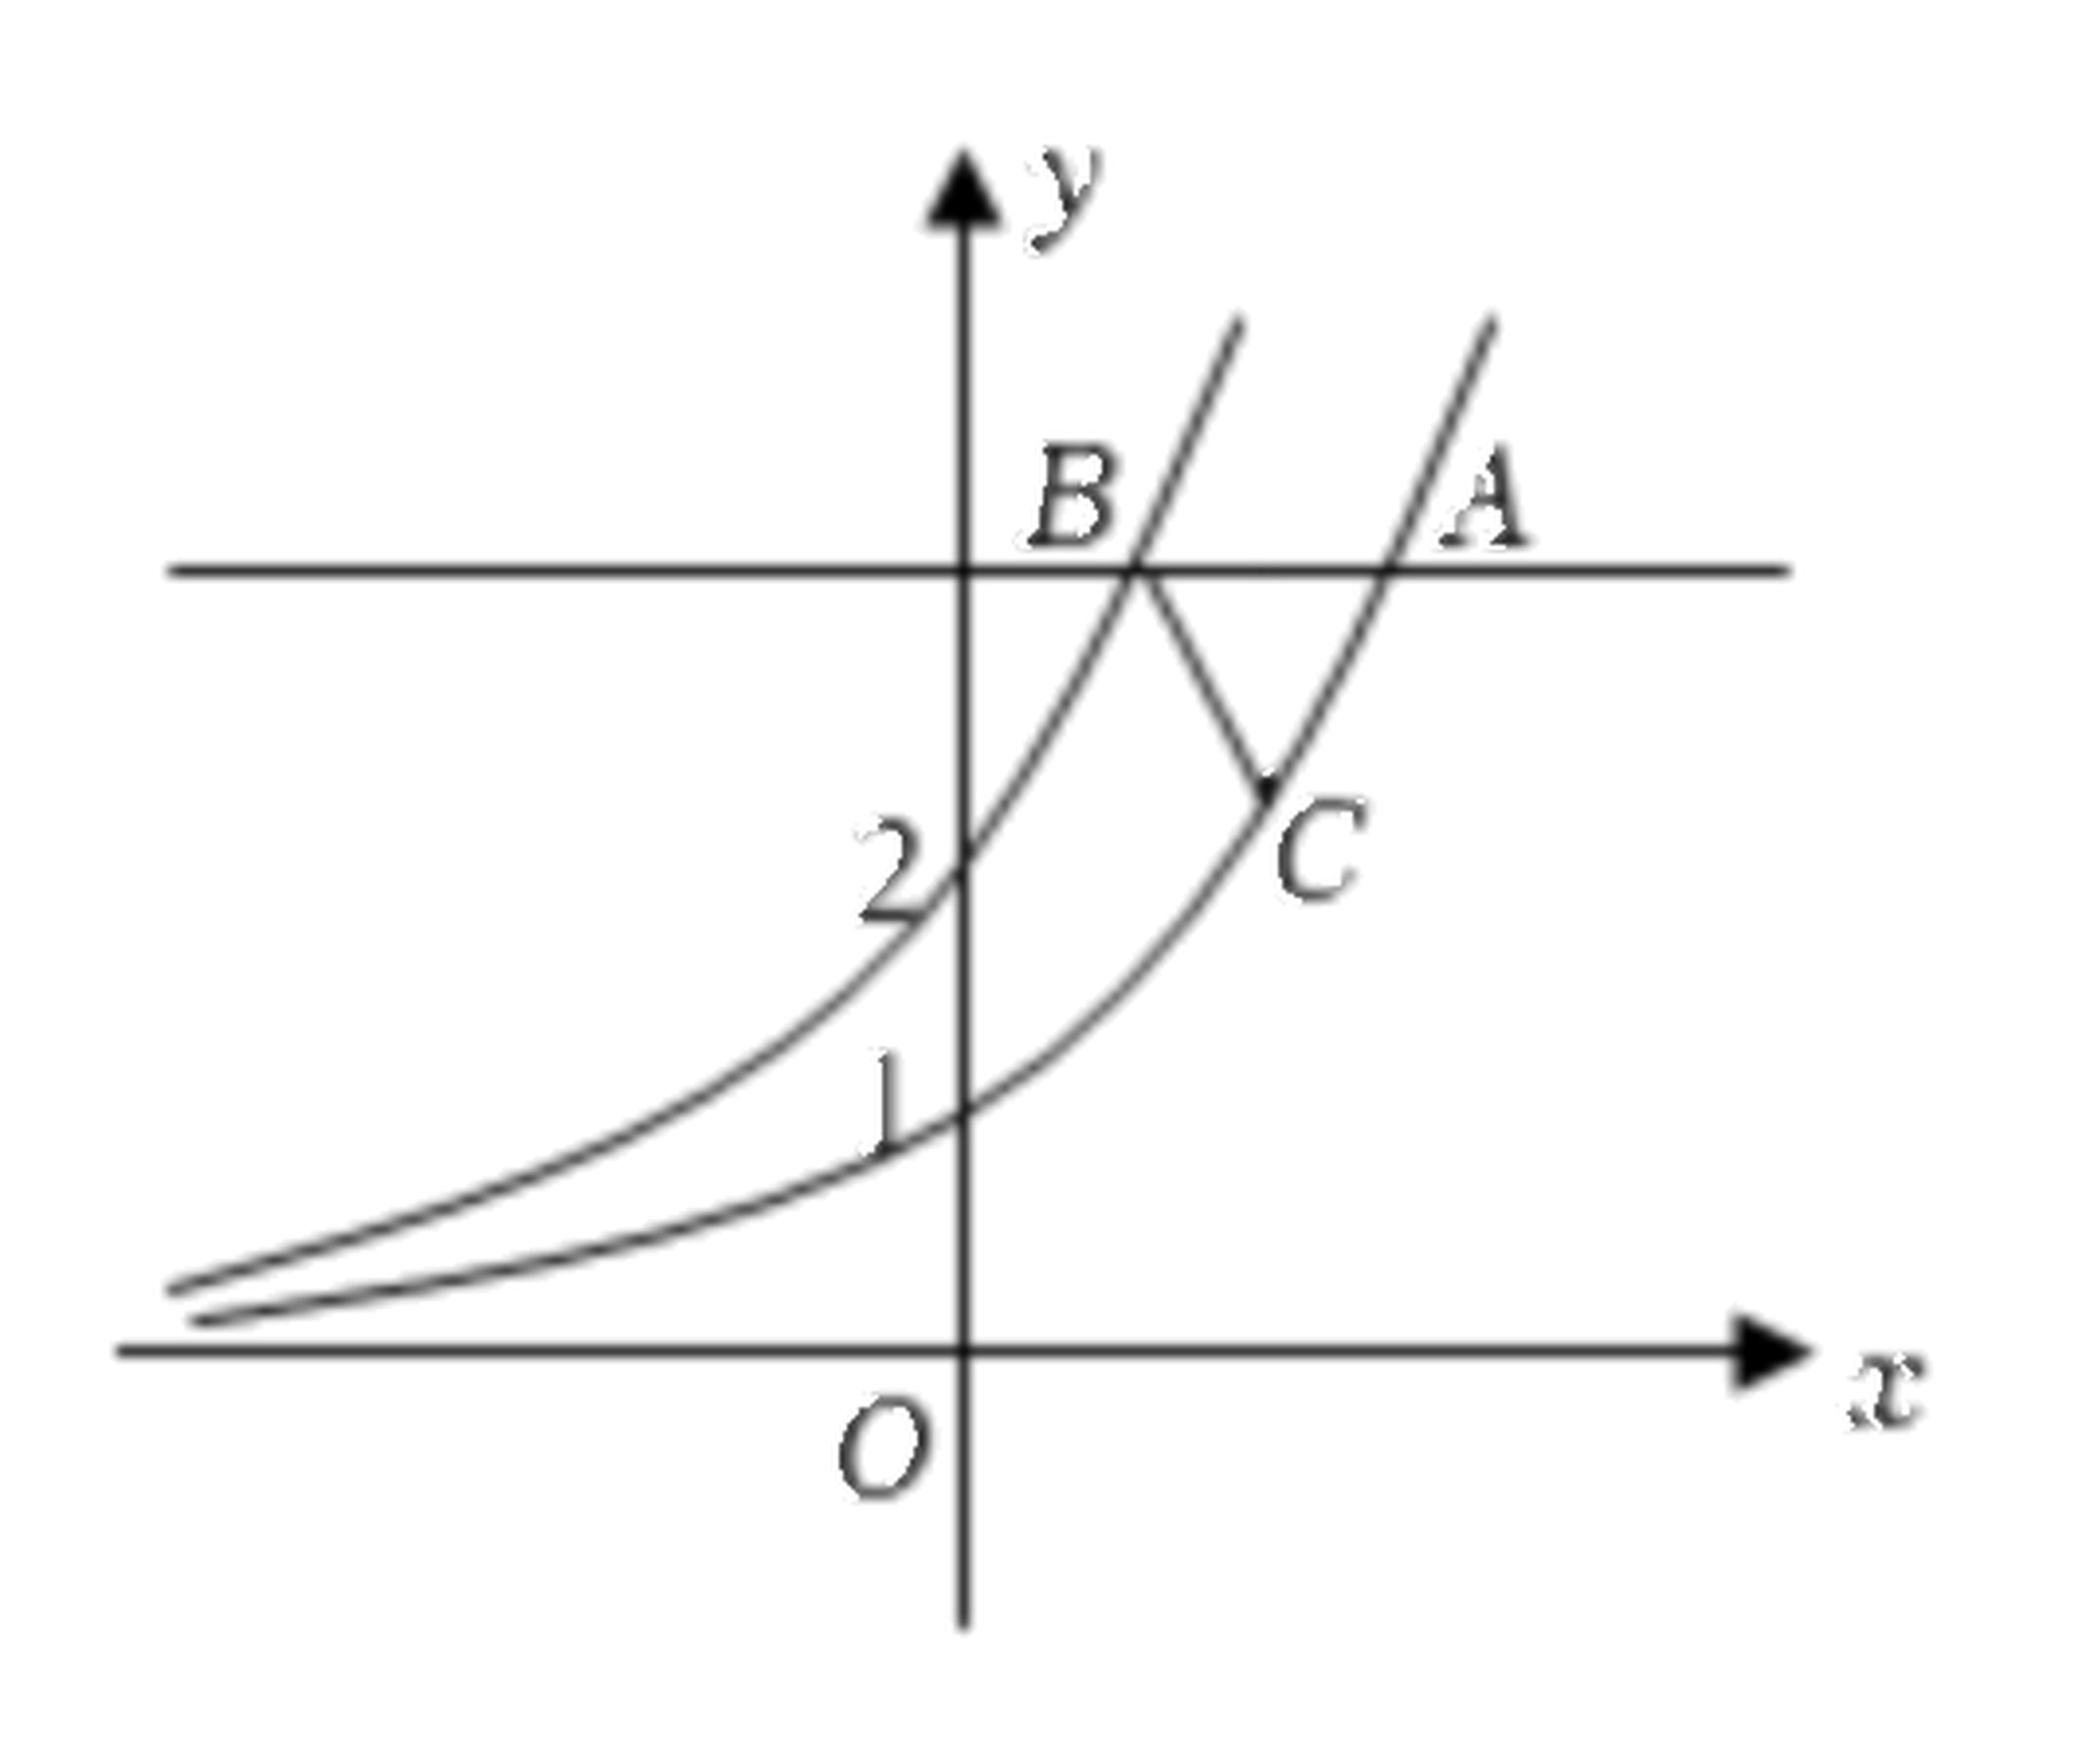
\includegraphics[width=0.40\textwidth]{figures/gao150_q11.png}
\end{center}

\ifanswer
\solbegin
\step{设直线 $l$ 的方程为 $y=a(a>0)$，}
\step{由 $2^x=a$，得 $x=\log_2 a$，所以 $A(\log_2 a,a)$，}
\step{由 $2^{x+1}=a$，得 $x=\log_2 a-1$，所以 $B(\log_2 a-1,a)$，所以 $\lvert AB\rvert=1$，}
\step{取 $AB$ 的中点 $D$，连接 $CD$，如图所示，}
\step{因为 $\triangle ABC$ 为等边三角形，则 $CD\perp AB$，且 $\lvert CD\rvert=\dfrac{\sqrt3}{2}$，}
\step{所以 $C\left(\log_2 a-\dfrac{1}{2},a-\dfrac{\sqrt3}{2}\right)$，}
\step{因为点 $C$ 在函数 $y=2^x$ 的图像上，所以 $a-\dfrac{\sqrt3}{2}=2^{\log_2 a-\frac{1}{2}}=\dfrac{a}{\sqrt2}$，}
\step{解得 $a=\dfrac{\sqrt3}{2-\sqrt2}=\dfrac{\sqrt3(2+\sqrt2)}{4-2}=\sqrt3+\dfrac{\sqrt6}{2}$，}
\step{所以点 $C$ 的纵坐标为 $a-\dfrac{\sqrt3}{2}=\dfrac{\sqrt3+\sqrt6}{2}$.}
\solend
\fi

% === Q12 === 解析配图（高斯函数方格阴影，仅答案版出）；"数学王子"弯引号；cases 块整体算一个印刷行；解析 4 行
\item 小玲在研究数学发展史，特别崇拜近代数学奠基者之一、享有“数学王子”称号的德国数学家高斯. 为了纪念高斯，我们把取整函数 $y=[x]$ 称为高斯函数，其中 $[x]$ 表示不超过 $x$ 的最大整数，如 $[1.1]=1$，$[-1.1]=-2$，则点集 $P=\{(x,y)\mid [x]^2+[y]^2=1\}$ 所表示的平面区域的面积为\blankline[4.4em].

\ifanswer
\solbegin
\step{$[x]^2+[y]^2=1$ 由 $\begin{cases}[x]=0\\ {[y]=-1}\end{cases}$ 或 $\begin{cases}[x]=0\\ {[y]=1}\end{cases}$ 或 $\begin{cases}[x]=-1\\ {[y]=0}\end{cases}$ 或 $\begin{cases}[x]=1\\ {[y]=0}\end{cases}$ 四个平面区域组成，}
\step{即 $\begin{cases}0\leqslant x<1\\ -1\leqslant y<0\end{cases}$ 或 $\begin{cases}0\leqslant x<1\\ 1\leqslant y<2\end{cases}$ 或 $\begin{cases}-1\leqslant x<0\\ 0\leqslant y<1\end{cases}$ 或 $\begin{cases}1\leqslant x<2\\ 0\leqslant y<1\end{cases}$，}
\step{作出平面区域如图所示，平面区域由四个边长为 $1$ 的正方形组成，}
\begin{center}
% 高斯函数 [x]^2+[y]^2=1 方格阴影区域图取 04 页顶部，去粉色水印、去色、4× LANCZOS 放大；仅答案版出
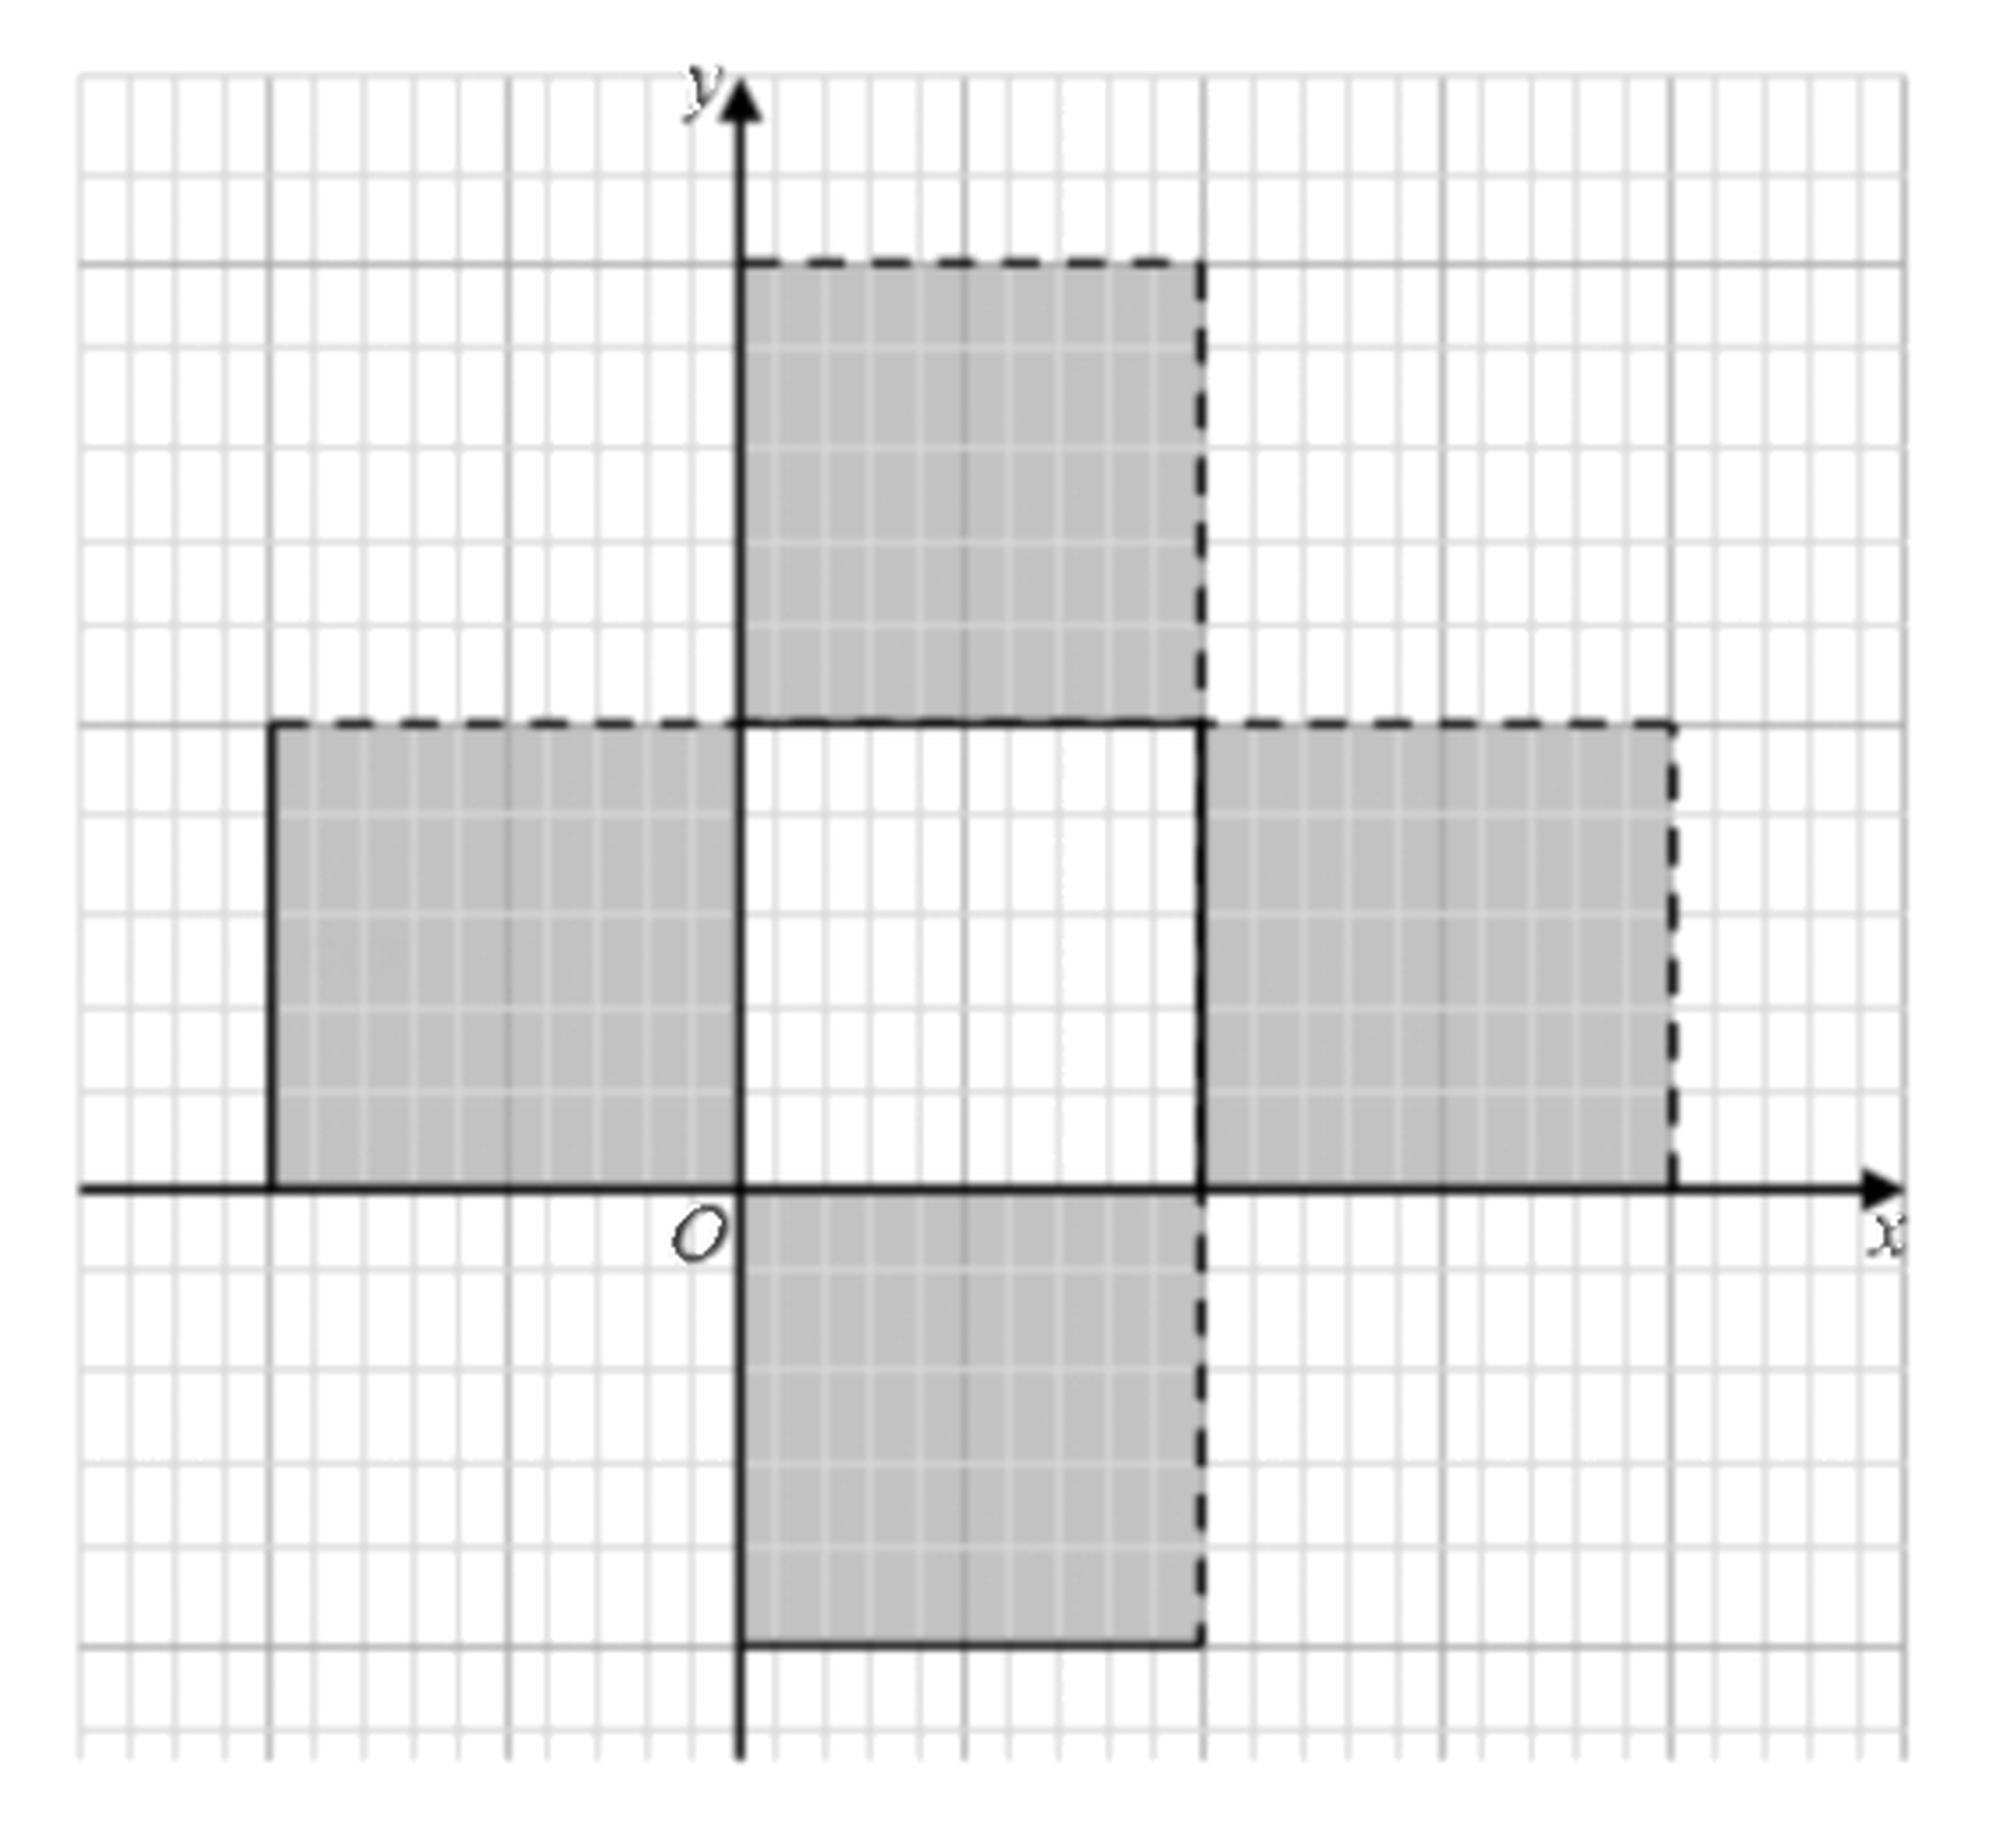
\includegraphics[width=0.34\textwidth]{figures/gao150_q12.png}
\end{center}
\step{总面积为 $1\times4=4$.}
\solend
\fi

\end{enumerate}

\bigsec{二、选择题}

\begin{enumerate}
\setcounter{enumi}{12}

% === Q13 === 答案在解析末句"故选 C"；括号 \mbox{（\quad）} 留空；四选项一行；解析 1 行
\item 设 $x\ne0$，则 $3^{\log_9 x^2}$ 的化简结果是\mbox{（\quad）}

\keepwithprev
A. $x$\qquad B. $\dfrac{1}{x}$\qquad C. $\lvert x\rvert$\qquad D. $\dfrac{1}{\lvert x\rvert}$

\ifanswer
\solbegin
\step{$3^{\log_9 x^2}=3^{\log_3\lvert x\rvert}=\lvert x\rvert$，故选 $C$.}
\solend
\fi

% === Q14 === 题目配图（两函数图像，三版都出）；\needvspace{8cm} 守卫放 \item 之前；"图像"照录；四选项两行两列；解析 2 行，故选 B
\needvspace{8cm}
\item 设 $a>0$ 且 $a\ne1$，$b\in\R$. 若函数 $y=a^{-\lvert x\rvert}$ 与 $y=x^b$ 的大致图像如图所示，则\mbox{（\quad）}

\keepwithprev
A. $0<a<1<b$\qquad\qquad B. $a>1$ 且 $b>1$

C. $0<a<1$ 且 $0<b<1$\qquad\qquad D. $0<b<1<a$

\begin{center}
% 两函数 y=a^{-|x|} 与 y=x^b 大致图像取 04 页右侧，去粉色水印、去色、4× LANCZOS 放大；三版都出
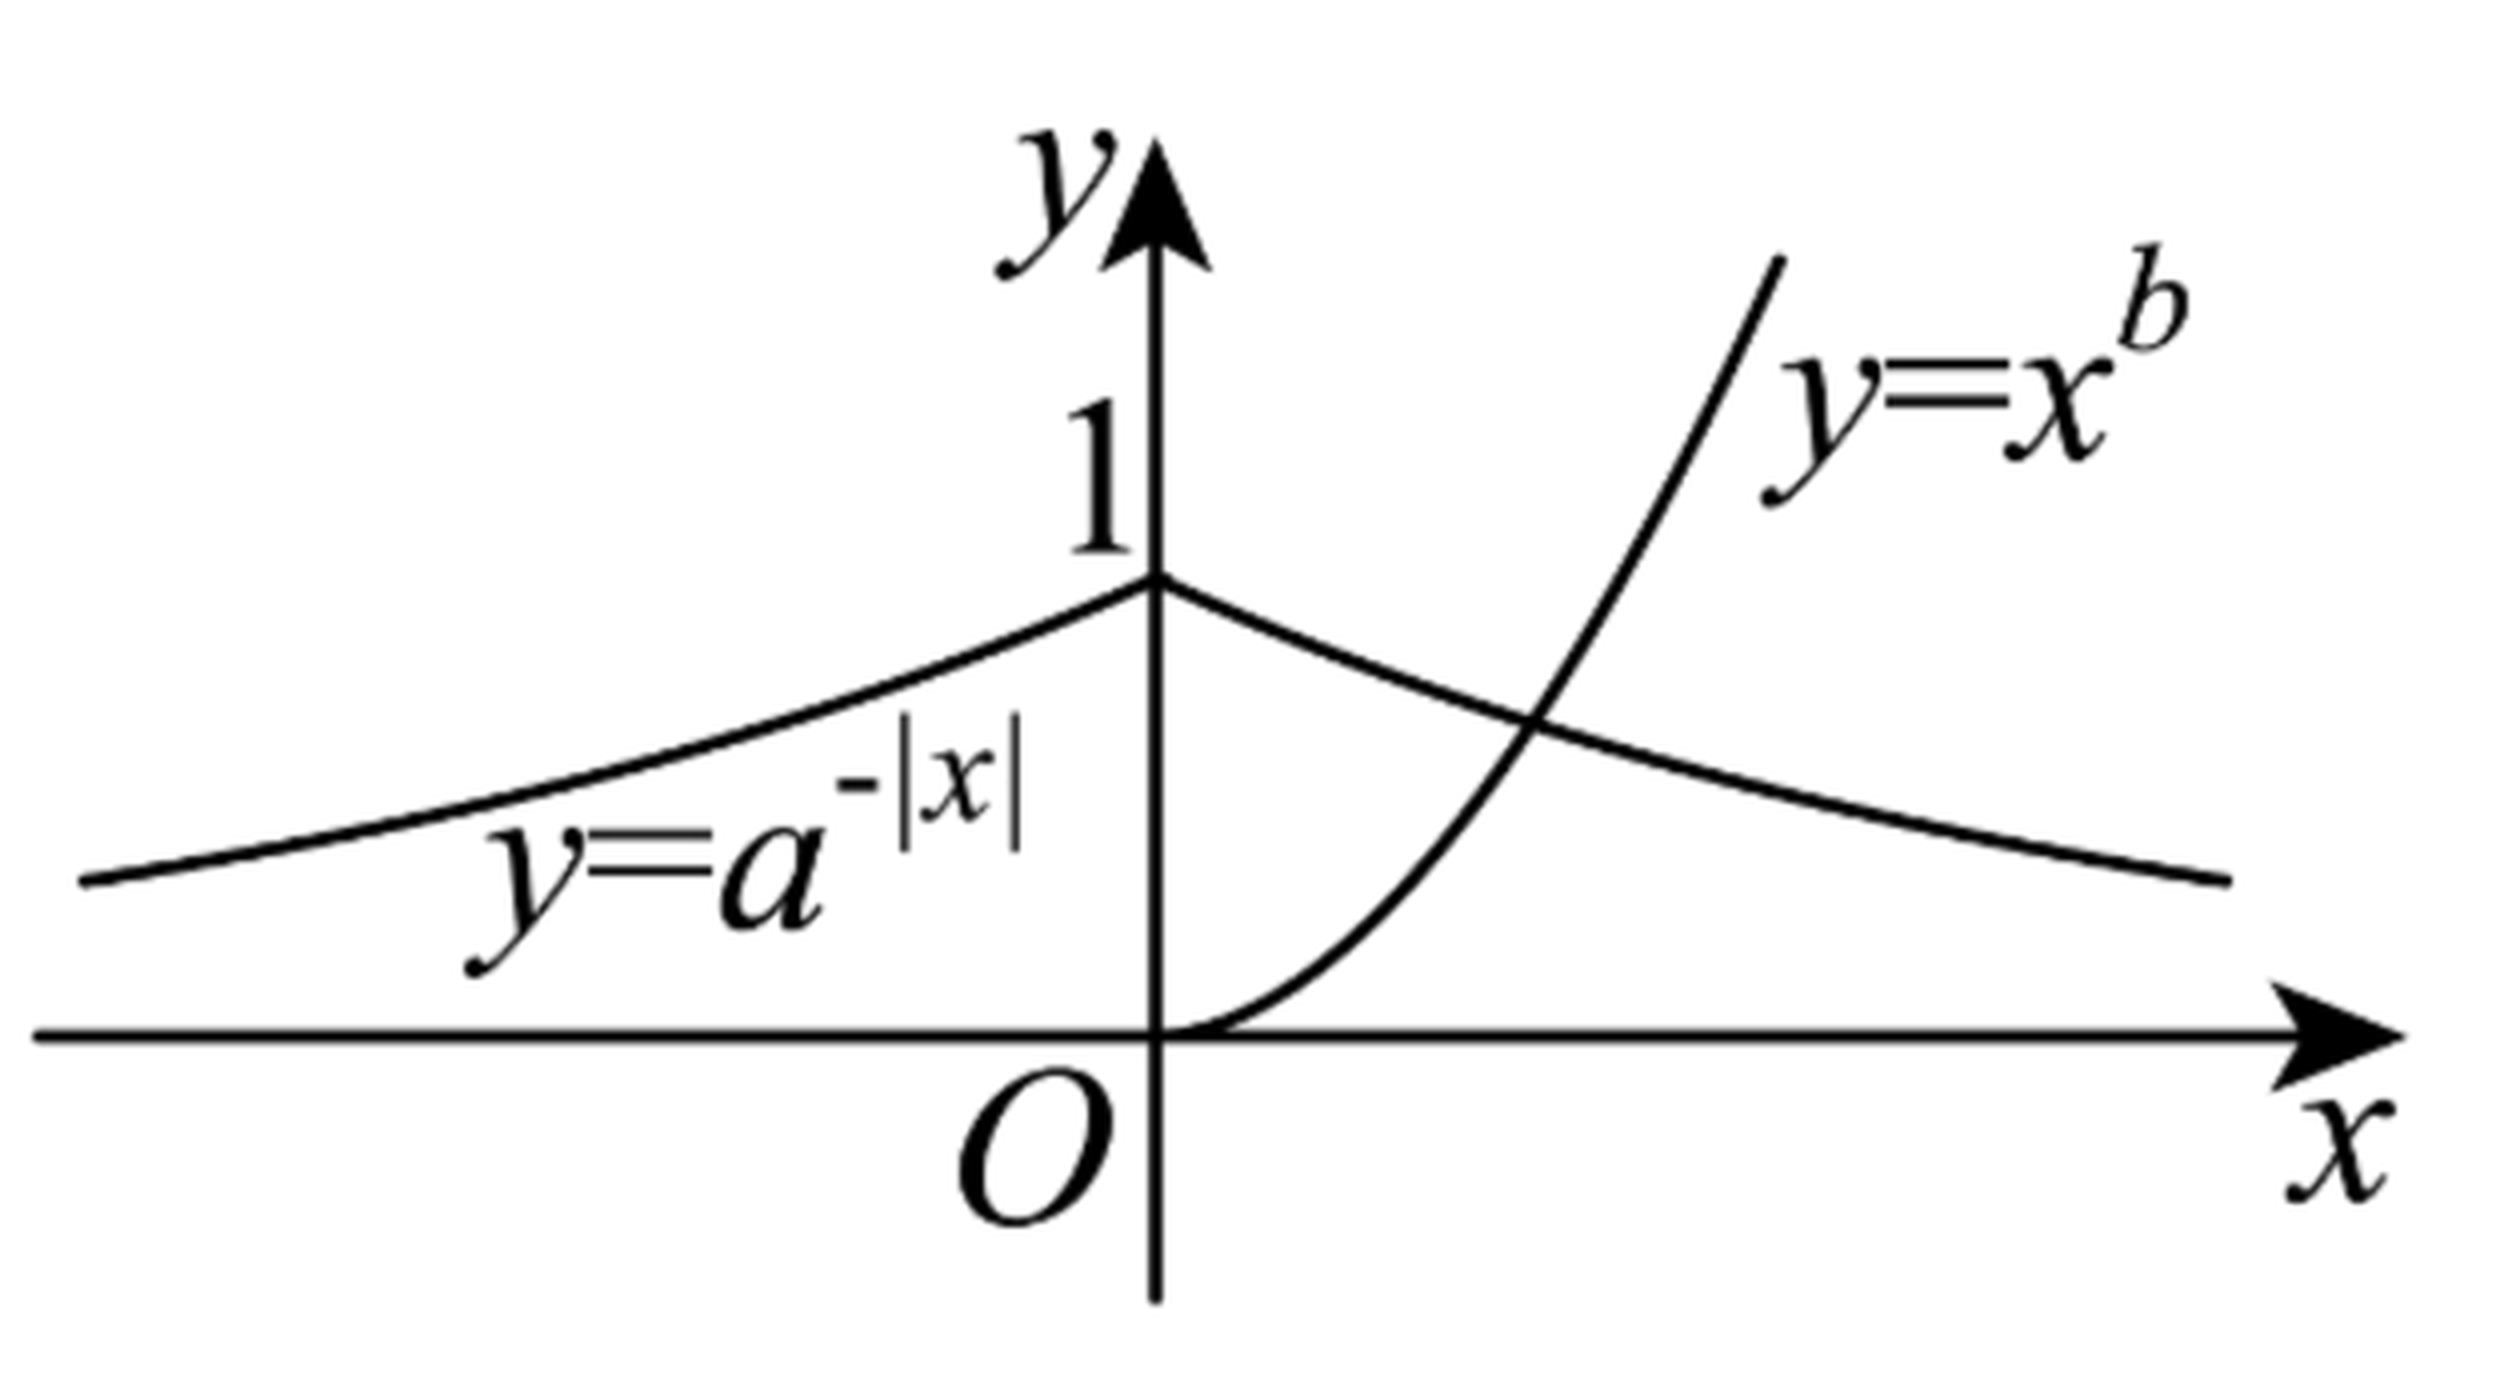
\includegraphics[width=0.40\textwidth]{figures/gao150_q14.png}
\end{center}

\ifanswer
\solbegin
\step{在 $(0,+\infty)$ 上，$y=a^{-x}$ 严格递减，得 $a>1$；}
\step{幂函数 $y=x^b$ 的图像递增且向上弯曲，得 $b>1$；故选 $B$.}
\solend
\fi

% === Q15 === "算术平均值／算术平均数"两处不同照录；四选项两行两列；解析 5 行（续 05 页顶），故选 B
\item 已知两个正数的算术平均值不小于它们的几何平均值，类比有以下结论：三个正数的算术平均数不小于它们的几何平均数，即当 $a,b,c$ 为正实数时，$\dfrac{a+b+c}{3}\geqslant\sqrt[3]{abc}$，当且仅当 $a=b=c$ 时等号成立. 利用上述结论，下列选项中判断正确的是\mbox{（\quad）}

\keepwithprev
A. 若 $x>0$，则 $2x+\dfrac{1}{x^2}\geqslant\dfrac{27}{8}$\qquad\qquad B. 若 $x>0$，则 $x^2+\dfrac{2}{x}\geqslant3$

C. 若 $0<x<1$，则 $x^2(1-x)\geqslant\dfrac{1}{9}$\qquad\qquad D. 若 $0<x<1$，则 $x^2(1-x)\leqslant\dfrac{1}{9}$

\ifanswer
\solbegin
\step{A：取 $x=1$，$2x+\dfrac{1}{x^2}=3<\dfrac{27}{8}$，错误.}
\step{B：$x^2+\dfrac{2}{x}=x^2+\dfrac{1}{x}+\dfrac{1}{x}\geqslant3\sqrt[3]{x^2\cdot\dfrac{1}{x}\cdot\dfrac{1}{x}}=3$，当且仅当 $x=1$ 时取等号，正确.}
\step{C：取 $x=\dfrac{1}{3}$，$x^2(1-x)=\dfrac{2}{27}<\dfrac{1}{9}$，错误.}
\step{D：取 $x=\dfrac{2}{3}$，$x^2(1-x)=\dfrac{4}{27}>\dfrac{1}{9}$，错误.}
\step{故选 $B$.}
\solend
\fi

% === Q16 === "完美集"新定义（弯引号、引号外空格照录）；圈数字①②文本模式；$n\in\N$；四选项两行两列；解析 9 行（6 行 05 页＋3 行 06 页顶），故选 A
\item 已知有限集 $A=\{a_1,a_2,\cdots,a_n\}$（$n\geqslant2$，$n\in\N$）. 若 $A$ 中元素 $a_i$（$i=1,2,\cdots,n$）满足 $a_1+a_2+\cdots+a_n=a_1\cdot a_2\cdots a_n$，就称 $A$ 为 “完美集”. 现有以下两个命题：

①恰有两个元素的 “完美集” 有无穷多个；

②若 $a_i$ 均为正整数，则 “完美集” $A$ 有且只有一个，且 $n=3$.

则\mbox{（\quad）}

\keepwithprev
A. ①和②都是真命题\qquad\qquad B. ①和②都是假命题

C. ①是真命题，②是假命题\qquad\qquad D. ①是假命题，②是真命题

\ifanswer
\solbegin
\step{①由 $a+b=ab\Leftrightarrow(a-1)(b-1)=1$，任取 $a>2$，则 $b=1+\dfrac{1}{a-1}\in(1,2)$，}
\step{得到无穷多个不同的完美集，①真.}
\step{②设 $1\leqslant a_1<a_2<\cdots<a_n$，则 $a_i\geqslant i$.}
\step{若 $n=2$，则 $(a_1-1)(a_2-1)=1$，只能有 $a_1=a_2=2$，与元素互异矛盾.}
\step{若 $n\geqslant4$，则 $a_1a_2\cdots a_n\geqslant a_2a_{n-1}a_n\geqslant2(n-1)a_n>na_n\geqslant a_1+\cdots+a_n$，矛盾.}
\step{当 $n=3$ 时，若 $a_1\geqslant2$，则 $a_1a_2a_3\geqslant6a_3>3a_3\geqslant a_1+a_2+a_3$，矛盾.}
\step{因此 $a_1=1$，$(a_2-1)(a_3-1)=2$，结合 $a_2<a_3$ 得 $a_2=2$，$a_3=3$.}
\step{唯一的完美集为 $\{1,2,3\}$，②真.}
\step{故选 $A$.}
\solend
\fi

\end{enumerate}

\bigsec{三、解答题}

\begin{enumerate}
\setcounter{enumi}{16}

% === Q17 === \varnothing 空集、$B\subseteq A$ 带下划线照录；弯引号内空格照录；解析 7 行
\item 设 $a,b\in\R$. 已知集合 $A=\{x\mid ax^2+3x-a>3\}$，$B=\{x\mid bx=1\}$.

(1) 若 $A=(1,2)$，求 $a$ 的值；

(2) 若 $a=0$，且 “ $x\in A$ ” 是 “ $x\in B$ ” 的必要非充分条件，求 $b$ 的取值范围.

\ifanswer
\solbegin
\step{(1) $A=(1,2)$，则 $a<0$，且 $1,2$ 是方程 $ax^2+3x-a-3=0$ 的两根.}
\step{由 $4a+6-a-3=0$，得 $a=-1$，此时不等式为 $-(x-1)(x-2)>0$，}
\step{解集确为 $(1,2)$.}
\step{(2) $a=0$ 时，$A=(1,+\infty)$，题意等价于 $B\subseteq A$ 且 $B\ne A$.}
\step{当 $b=0$ 时，$B=\varnothing$，符合条件.}
\step{当 $b\ne0$ 时，$B=\left\{\dfrac{1}{b}\right\}$，条件等价于 $\dfrac{1}{b}>1$，解得 $0<b<1$.}
\step{因此 $b$ 的取值范围为 $[0,1)$.}
\solend
\fi

% === Q18 === $p\in\Z$；"图像"（像，有亻）照录；指数 $-2p^2+5p$；解析 8 行（(1) 首行 06 页末＋2 行 07 页顶、(2) 5 行 07 页）
\item 设 $p\in\Z$，已知 $f(x)=x^{-2p^2+5p}$.

(1) 若幂函数 $y=f(x)$ 的图像关于原点成中心对称，且满足 $f(3)<f(4)$，求 $p$ 的值；

(2) 当 $p=-2$ 时，求满足 $f(2x+3)<f(x-4)$ 的 $x$ 的取值范围.

\ifanswer
\solbegin
\step{(1) 图像关于原点成中心对称，得整数 $-2p^2+5p$ 为奇数.}
\step{由 $f(3)<f(4)$，得 $-2p^2+5p>0\Leftrightarrow0<p<\dfrac{5}{2}$，}
\step{结合 $p\in\Z$，得 $p=1$ 或 $p=2$，对应指数分别为 $3$、$2$，所以 $p=1$.}
\step{(2) 当 $p=-2$ 时，$f(x)=\dfrac{1}{x^{18}}$，定义域为 $\{x\in\R\mid x\ne0\}$.}
\step{原不等式要求 $x\ne-\dfrac{3}{2}$ 且 $x\ne4$，}
\step{此时 $\dfrac{1}{(2x+3)^{18}}<\dfrac{1}{(x-4)^{18}}\Leftrightarrow\lvert 2x+3\rvert>\lvert x-4\rvert\Leftrightarrow(2x+3)^2>(x-4)^2$，}
\step{因此 $(x+7)(3x-1)>0\Leftrightarrow x<-7$ 或 $x>\dfrac{1}{3}$，}
\step{排除 $x=4$，得 $x\in(-\infty,-7)\cup\left(\dfrac{1}{3},4\right)\cup(4,+\infty)$.}
\solend
\fi

% === Q19 === $a\in\R$、$g(x)=f(2x+1)+a\cdot f(x)+2$；解析 6 行（(2) 末两行续 08 页顶）
\item 已知 $f(x)=2^x$.

(1) 求方程 $f(2x)-f(x)=6$ 的解；

(2) 设 $a\in\R$，$g(x)=f(2x+1)+a\cdot f(x)+2$，若对于任意 $x\in[-1,1]$，均有 $g(x)\geqslant1$，求 $a$ 的取值范围.

\ifanswer
\solbegin
\step{(1) 令 $t=2^x>0$，则 $t^2-t-6=(t-3)(t+2)=0$，}
\step{由 $t>0$ 得 $t=3$，所以 $x=\log_2 3$.}
\step{(2) 令 $t=2^x$，则 $t\in\left[\dfrac{1}{2},2\right]$，且 $g(x)\geqslant1\Leftrightarrow2t^2+at+1\geqslant0\Leftrightarrow a\geqslant-\left(2t+\dfrac{1}{t}\right)$，}
\step{由基本不等式得 $2t+\dfrac{1}{t}\geqslant2\sqrt{2t\cdot\dfrac{1}{t}}=2\sqrt2$，}
\step{当且仅当 $t=\dfrac{1}{\sqrt2}\in\left[\dfrac{1}{2},2\right]$ 时等号成立，}
\step{因此 $-\left(2t+\dfrac{1}{t}\right)$ 的最大值为 $-2\sqrt2$，所求范围为 $a\in[-2\sqrt2,+\infty)$.}
\solend
\fi

% === Q20 === "极闭集"新定义、3 问，全卷末题；$M\subseteq(0,+\infty)$ 带下划线照录；自定义运算 $x*y$ 星号照录；解析 13 行（9 行 08 页＋4 行 09 页上半）
\item 对于非空实数集 $M\subseteq(0,+\infty)$，若满足以下两个条件：

① $M$ 中至少含有 $2$ 个元素，且 $1\notin M$；

②对于 $M$ 中任意两个不相等的元素 $x$、$y$，定义 $x*y=\dfrac{xy+1}{x+y}$，且 $x*y\in M$.

则称 $M$ 为 “极闭集”.

(1) 分别判断集合 $A=\left\{\dfrac{1}{2},3\right\}$ 与集合 $B=(1,+\infty)$ 是否为 “极闭集” （无需理由）；

(2) 若 $M$ 是 “极闭集”，证明：$M$ 中不可能所有元素都小于 $1$；

(3) 证明：不存在任何有限集是 “极闭集”.

\ifanswer
\solbegin
\step{(1) $A$ 不是 “极闭集”，$B$ 是 “极闭集”.}
\step{(2) 假设 $M$ 中所有元素都小于 $1$，取其中两个不相等的元素 $x$、$y$，}
\step{则 $x*y-1=\dfrac{(1-x)(1-y)}{x+y}>0$，}
\step{这与 $x*y\in M$ 且 $M$ 中所有元素都小于 $1$ 矛盾.}
\step{(3) 假设有限集 $M$ 是 “极闭集”，}
\step{由 (2) 及 $1\notin M$，得 $M$ 中存在大于 $1$ 的元素.}
\step{若 $M$ 中有小于 $1$ 的元素，取其中最大的一个为 $a$，另取 $b\in M$ 且 $b>1$，}
\step{则 $a*b-a=\dfrac{1-a^2}{a+b}>0, a*b-1=\dfrac{(a-1)(b-1)}{a+b}<0$，}% 半角逗号在两个数学式组之间，全稿惯例、非笔误，照录
\step{于是 $a<a*b<1$ 且 $a*b\in M$，与 $a$ 的最大性矛盾.}
\step{若 $M$ 中没有小于 $1$ 的元素，则 $M\subseteq(1,+\infty)$.}
\step{取 $a=\min M$，另取 $b\in M$ 且 $b\ne a$，则 $a*b-a=\dfrac{1-a^2}{a+b}<0$，}
\step{于是 $a*b<a$ 且 $a*b\in M$，与 $a$ 的最小性矛盾.}
\step{因此不存在任何有限集是 “极闭集”.}
\solend
\fi

\end{enumerate}

\end{document}
